\documentclass[11pt,a4paper]{book}
\usepackage{mathpazo}
\usepackage[utf8]{inputenc}
\usepackage[T1]{fontenc}
\usepackage[dutch]{babel}
\usepackage{amsmath,amssymb,amsthm}
\usepackage{mathtools}
\usepackage{physics}
\usepackage{geometry}
\geometry{margin=2.5cm}
\usepackage{graphicx}
\usepackage{enumerate}
\usepackage{array}
\usepackage{booktabs}
\usepackage{siunitx}
\usepackage[labelfont=bf,font=small,width=0.85\linewidth]{caption}

\usepackage{xcolor}
\definecolor{chaptergrey}{gray}{0.3}
\usepackage[palatino, nogrey]{quotchap}
\renewcommand*{\sectfont}{\bfseries\sffamily}

\usepackage{fancyhdr}
\pagestyle{fancy}
\fancyhf{} % Clear old header/footer settings
\fancypagestyle{plain}{%dit is om de eerste pagina van een hoofdstuk identiek te maken aan de andere
  \fancyfoot[C]{-- \thepage \,--} % Set your preferred page number position (e.g., center footer)
  \renewcommand{\headrulewidth}{0pt} % Set to 0pt if you want no header line
  \renewcommand{\footrulewidth}{0pt} % Adjust footer line width if needed
}
\fancyfoot[C]{-- \thepage \,--}
%\fancyhead[R]{\thepage} % Zet het paginanummer rechts in de header
\renewcommand{\headrulewidth}{0pt} % Verwijder de horizontale lijn onder de header

\usepackage[version=4]{mhchem}
\usepackage{hyperref}

\usepackage{enumitem}
 \setlist[enumerate]{topsep=3pt,itemsep=0.2ex,partopsep=0.3ex,parsep=0.2ex}
 \setlist[itemize]{topsep=3pt,itemsep=0.2ex,partopsep=0.3ex,parsep=0.2ex}
 \setlist[description]{topsep=6pt,itemsep=0.2ex,partopsep=0.3ex,parsep=0.2ex}
 %\setlist[list]{topsep=6pt,itemsep=-1ex,partopsep=1ex,parsep=1ex}

\usepackage{a4wide}
\usepackage{cite}
\usepackage{hhline}     % generates nicer table lines (without missing pixels) + more flexible

\widowpenalty=10000
\clubpenalties 5 10000 10000 10000 10000 0
\raggedbottom

\makeatother

\sisetup{output-decimal-marker={.}, group-separator={\,}}

\usepackage[most]{tcolorbox}
%\tcbuselibrary{skins}
\tcbuselibrary{breakable}

\newtcolorbox{toepassing}[1]{breakable, colback=blue!2!white,colframe=blue!50!black,fonttitle=\bfseries,title={Toepassing: #1}}
\newtcolorbox{voorbeeld}[1]{breakable, colback=green!2!white,colframe=green!50!black,fonttitle=\bfseries,title={Voorbeeld: #1}}
\newtcolorbox{definitie}[1]{breakable, colback=yellow!2!white,colframe=yellow!60!black,fonttitle=\bfseries,title={Definitie: #1}}
\newtcolorbox{besluit}[1]{breakable, colback=gray!2!white,colframe=gray!50!black,fonttitle=\bfseries,title={Besluit: #1}}
\newtcolorbox{samenvatting}[1]{breakable, colback=orange!3!white,colframe=orange!60!black,fonttitle=\bfseries,title={Samenvatting: #1}}
\newtcolorbox{reflectie}[1]{breakable, colback=violet!3!white,colframe=violet!50!black,fonttitle=\bfseries,title={Reflectievragen: #1}}

\newcounter{oefeningcounter}[chapter]
\renewcommand{\theoefeningcounter}{\thechapter.\arabic{oefeningcounter}}

% definitie van de omgeving
\newenvironment{oefening}[1][]{%
  \par\vspace{0.8em} % witruimte vóór oefening
  \noindent\refstepcounter{oefeningcounter}%
  \textbf{Oefening \theoefeningcounter%
  \ifx\relax#1\relax\else\ (#1)\fi}\par\vspace{0.4em}
}{%
  \par\vspace{0.8em} % witruimte na oefening
}
%%%%%

%\newcommand{\dx}[1]{\,\mathrm{d}#1}
%\newcommand{\dG}{\,\mathrm{d}G}
%\newcommand{\dH}{\,\mathrm{d}H}
%\newcommand{\dU}{\,\mathrm{d}U}
%\newcommand{\dS}{\,\mathrm{d}S}
%\newcommand{\dQ}{\delta Q}
%\newcommand{\dW}{\delta W}
%\newcommand{\dT}{\,\mathrm{d}T}
%\newcommand{\dp}{\,\mathrm{d}p}
%\newcommand{\dV}{\,\mathrm{d}V}

%\title{\textbf{Fysico Chemie} \\ Chemische Thermodynamica voor Industrieel Ingenieurs}
%\author{Stijn De Jonge \\ KU Leuven \\ Faculteit Industri\"ele Ingenieurswetenschappen}
%\date{2026}

%%%%% Online versie (Quarto-site) %%%%%
% Deze LaTeX is de enige bron: bij elke wijziging wordt de site automatisch opnieuw gemaakt.
% Figuren uit Python staan in de map Figuren/ (worden automatisch bijgewerkt, niet zelf aanpassen):
%     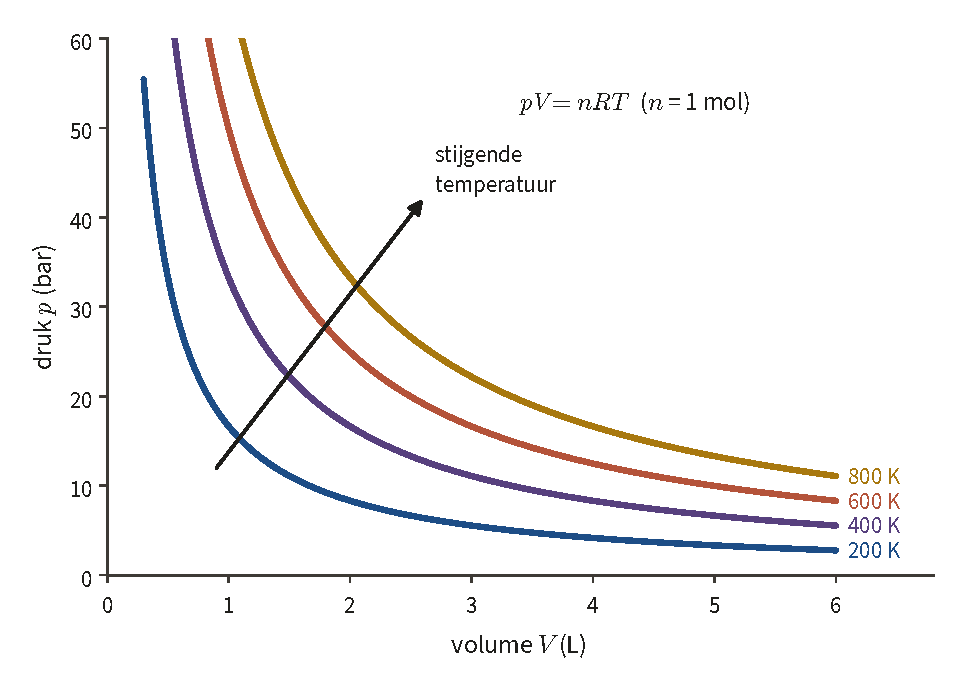
\includegraphics[width=0.7\linewidth]{Figuren/boyle}
% Een gewenste, nog niet bestaande figuur: verwijs naar een bestand dat nog niet bestaat en
% beschrijf in het bijschrift wat je wil zien. In de PDF verschijnt dan een kader i.p.v. een fout.
% Een interactief onderdeel (enkel online), bv. in Kinetica:  \interactief{arrhenius}
\newcommand{\interactief}[1]{%
  \begin{tcolorbox}[colback=gray!3!white,colframe=gray!40!white,boxrule=0.4pt,arc=2mm]
  \small\textbf{Probeer zelf online.} Bij dit onderdeel hoort een interactieve figuur op de cursussite: \url{https://dejonges.github.io/fysicochemie-cursus/}
  \end{tcolorbox}}
\let\origincludegraphics\includegraphics
\renewcommand{\includegraphics}[2][]{%
  \IfFileExists{#2}{\origincludegraphics[#1]{#2}}{%
  \IfFileExists{#2.pdf}{\origincludegraphics[#1]{#2}}{%
  \IfFileExists{#2.png}{\origincludegraphics[#1]{#2}}{%
  \fbox{\parbox[c][3cm][c]{0.6\linewidth}{\centering\small\itshape Figuur in voorbereiding\\[2pt]\upshape\footnotesize\detokenize{#2}}}}}}}
% Uitwerking van een oefening: enkel op de website (dichtgeklapt), niet in het boek.
%     \begin{oefening} ... \end{oefening}
%     \begin{oplossing} ... \end{oplossing}
\usepackage{environ}
\NewEnviron{oplossing}{}
%%%%%

\begin{document}

\frontmatter

\begin{titlepage}
\centering
\vspace*{3cm}
{\Huge\bfseries Fysico Chemie\par}
\vspace{1cm}
{\Large Chemische Thermodynamcia voor Industrieel Ingenieurs\par}
\vfill
{\Large Stijn De Jonge\par}
\vspace{0.5cm}
KU Leuven\\
Faculteit Industriële Ingenieurswetenschappen\\
%\vfill
\vspace{0.5cm}
{Academiejaar 2026-2027}
\end{titlepage}

\tableofcontents
\mainmatter

%==============================================================================
\chapter{Energie en de eerste hoofdwet van de thermodynamica}
\label{ch:energie}
%==============================================================================

\section{Waarom thermodynamica?}

Een procesingenieur moet een gascompressor dimensioneren. Al bij de eerste simulaties blijkt dat het gas tijdens de compressie sterk opwarmt. Dat verkort de levensduur van de machine, stelt hogere eisen aan de materialen en kost extra energie. Daarom bouwt men industri\"ele compressoren op uit meerdere trappen met tussenkoeling. Waarom warmt een gas op bij compressie? Hoeveel arbeid kost het? Waarom bespaart tussenkoeling vermogen? En wanneer mag je het gas nog als ideaal beschouwen?

Al deze vragen worden beantwoord door de \emph{thermodynamica}: de leer van hoe energie wordt opgeslagen, uitgewisseld en omgezet. Zonder thermodynamica kan je geen warmtewisselaar, destillatiekolom, reactor of koelinstallatie rationeel ontwerpen. Het bijzondere is dat ze geen kennis van individuele moleculen vereist: een handvol macroscopische grootheden (temperatuur, druk, volume, samenstelling) volstaat om zeer complexe processen nauwkeurig te voorspellen.

\section{Het thermodynamisch systeem}

Elke analyse begint met het afbakenen van het \emph{systeem}. Alles daarbuiten is de \emph{omgeving}; de scheiding is de \emph{systeemgrens}. Die keuze lijkt triviaal, maar alle massa- en energiebalansen hangen ervan af. Figuur~\ref{fig:systemen} toont de vier types, ingedeeld volgens wat de grens mag oversteken.

\begin{figure}[htb]
    \centering
    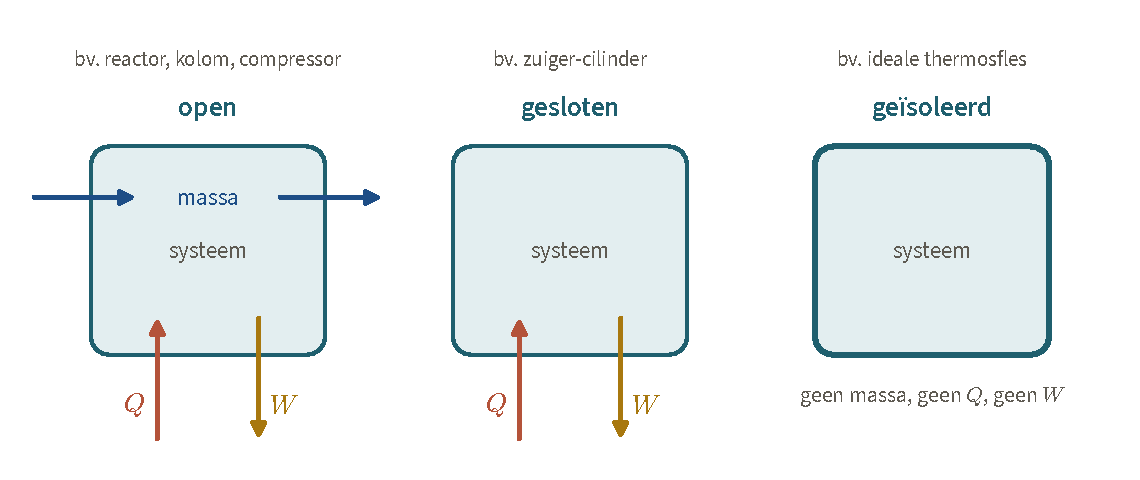
\includegraphics[width=0.9\linewidth]{Figuren/systemen}
    \caption{Open, gesloten, adiabatisch en ge\"isoleerd systeem. Een open systeem wisselt massa en energie uit, een gesloten systeem enkel energie (warmte $Q$ en arbeid $W$), een adiabatisch systeem enkel arbeid, een ge\"isoleerd systeem niets.}
    \label{fig:systemen}
\end{figure}

\begin{itemize}
\item Een \emph{gesloten systeem}, zoals gas in een zuiger-cilinder, wisselt geen massa uit, wel warmte en arbeid. De basiswetten leiden we eerst af voor gesloten systemen.
\item Een \emph{open systeem} laat ook massa door. Bijna elk industrieel toestel is open: pompen, compressoren, warmtewisselaars, kolommen, reactoren. De stromen voeren energie mee, en daarvoor zullen we de \emph{enthalpie} nodig hebben (\S~\ref{sec:enthalpie}).
\item Een \emph{adiabatisch systeem} heeft een grens die geen warmte doorlaat ($Q = 0$), maar wel arbeid. Dat gebeurt bij goede isolatie, maar ook als een proces zo snel verloopt dat er geen tijd is voor warmte-uitwisseling: de compressie in een fietspomp of dieselmotor, of een gas dat door een compressor stroomt. Alle arbeid blijft dan in het systeem en verhoogt de temperatuur (figuur~\ref{fig:compressie}). Hetzelfde geldt voor een goed ge\"isoleerde reactor, die opwarmt door zijn eigen reactiewarmte (\S~\ref{sec:warmte-effecten}). Adiabatisch zegt enkel iets over warmte: een adiabatisch systeem kan zowel open als gesloten zijn.
\item Een \emph{ge\"isoleerd systeem} wisselt helemaal niets uit. Het universum als geheel is het enige echte voorbeeld; een thermosfles of een calorimeter benadert het.
\end{itemize}


\section{Thermodynamisch evenwicht}

Een systeem laat zich pas eenduidig beschrijven als het in \emph{thermodynamisch evenwicht} is: na verloop van tijd zijn alle lokale verschillen in druk, temperatuur en samenstelling verdwenen. Daarvoor zijn drie voorwaarden nodig.
\begin{itemize}
\item \textbf{Thermisch evenwicht}: geen netto warmtestroom meer, dus overal dezelfde temperatuur.
\item \textbf{Mechanisch evenwicht}: geen netto kracht, bv.\ een zuiger staat stil als $p = p_\text{ext}$.
\item \textbf{Chemisch evenwicht}: de samenstelling verandert niet meer. Bij \ce{N2 + 3H2 <=> 2NH3} lopen heen- en terugreactie even snel; op moleculaire schaal gaat de reactie door, macroscopisch staat alles stil (\emph{dynamisch evenwicht}).
\end{itemize}

\begin{definitie}{Nulde hoofdwet van de thermodynamica}
Als systeem $A$ in thermisch evenwicht is met $C$, en $B$ ook met $C$, dan zijn $A$ en $B$ onderling in thermisch evenwicht.
\end{definitie}

Deze vanzelfsprekende uitspraak is de basis van elke temperatuurmeting: de thermometer speelt de rol van $C$.

\section{Toestandsvariabelen}

Een industri\"ele reactor van $100~\mathrm{m^3}$ bevat meer dan $10^{30}$ moleculen, maar zijn toestand ligt vast door enkele \emph{toestandsvariabelen}: druk, temperatuur, volume en samenstelling. We moeten dus niet de toestand van iedere molecule individueel bestuderen.

\subsection{Intensieve en extensieve grootheden}

Een \emph{extensieve grootheid} verdubbelt als je twee identieke systemen samenvoegt: massa $m$, volume $V$, hoeveelheid stof $n$, interne energie $U$, enthalpie $H$, entropie $S$. 

Een \emph{intensieve grootheid} hangt niet af van de grootte: temperatuur $T$, druk $p$, dichtheid $\rho$, concentratie, en elke molaire grootheid zoals $V_\mathrm{m} = V/n$. In een warmtewisselaar is het temperatuurverschil (intensief) de drijvende kracht, terwijl de overgedragen warmte (extensief) schaalt met het debiet.

\subsection{Toestandsfuncties en padfuncties}

Een \emph{toestandsfunctie} hangt enkel af van de toestand van het systeem, niet van de weg waarlangs die bereikt werd. De interne energie is er een voorbeeld hiervan: $\Delta U = U_2 - U_1$, welke weg je ook volgt. Hetzelfde geldt voor $H$, $S$ en $G$. Warmte en arbeid zijn daarentegen \emph{padfuncties}: hun waarde hangt af van het proces (figuur~\ref{fig:padfunctie}). Daarom schrijven we $\dd U$ (exacte differentiaal) maar $\delta Q$ en $\delta W$.

\begin{figure}[htb]
    \centering
    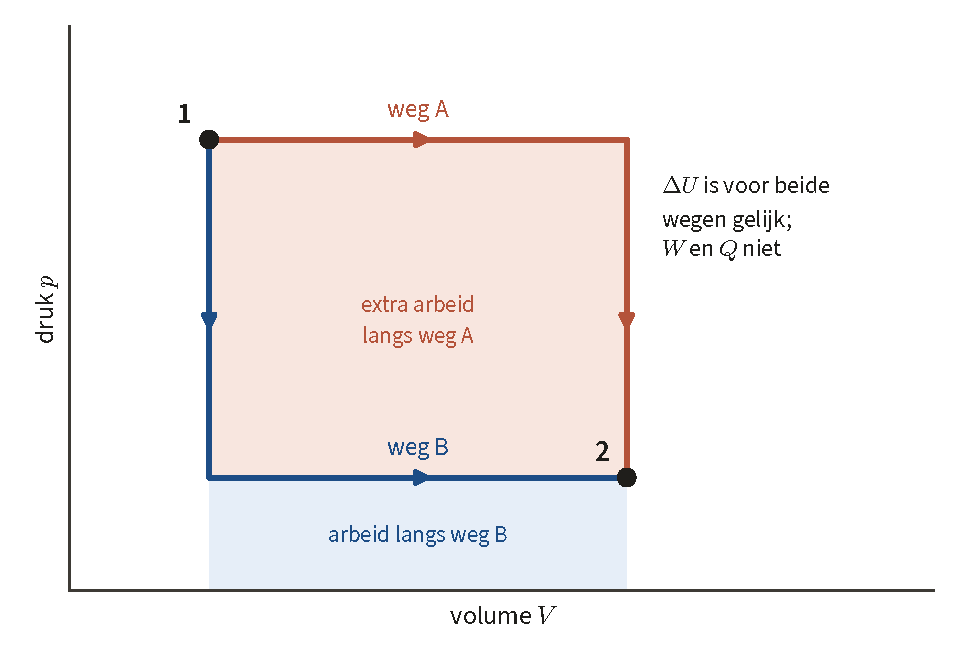
\includegraphics[width=0.7\linewidth]{Figuren/padfunctie}
    \caption{Twee wegen van toestand 1 naar toestand 2. De arbeid die het gas levert, is de oppervlakte onder de curve en is langs weg A veel groter. Omdat $\Delta U$ voor beide wegen gelijk is, moet ook de uitgewisselde warmte verschillen.}
    \label{fig:padfunctie}
\end{figure}

Je kan ook toepassen op zeer alledaagse situaties. Rij met de auto van een bergtop A naar het dal B en terug. De barometer toont in A voor en na de rit dezelfde druk: de luchtdruk is een toestandsfunctie. De brandstofmeter niet: hoeveel benzine je verbruikt hebt, hangt af van de gekozen route.


\section{Toestandsvergelijkingen}

Toestandsvariabelen zijn niet onafhankelijk: een \emph{toestandsvergelijking} verbindt ze. De eenvoudigste toestandsvergelijk is de ideale gaswet.

\subsection{De ideale gaswet}

Voor een verdund gas geldt
\begin{equation}
pV = nRT,
\end{equation}
met $R = \SI{8.314}{\joule\per\mole\per\kelvin}$ (in SI-eenheden; met bar en liter wordt dat \SI{0.08314}{\litre\bar\per\mole\per\kelvin}). De ideale gaswet is een \emph{limietwet}: elk gas voldoet aan deze toestandsvergelijk in de limiet $p \to 0$, en elke betere toestandsvergelijking moet in die limiet tot $pV = nRT$ herleiden.


\subsection{De ideale gaswet vanuit de moleculen: kinetische gastheorie}
\label{sec:kinetische-gastheorie}

De ideale gaswet werd experimenteel gevonden, maar ze laat zich ook afleiden uit een eenvoudig beeld van bewegende moleculen. Die afleiding is de moeite waard: ze toont wat druk en temperatuur op moleculair niveau \emph{betekenen}.

We maken drie aannames: 
\begin{enumerate}
    \item Het gas bestaat uit $N$ moleculen met massa $m$ die vrij en willekeurig door elkaar bewegen.
    \item De moleculen zelf nemen geen volume in.
    \item Er werken geen krachten tussen de moleculen; ze botsen enkel elastisch tegen de wand.
\end{enumerate}

De afleiding verloopt in drie stappen (figuur~\ref{fig:kmt-botsing}).

\begin{figure}[htb]
    \centering
    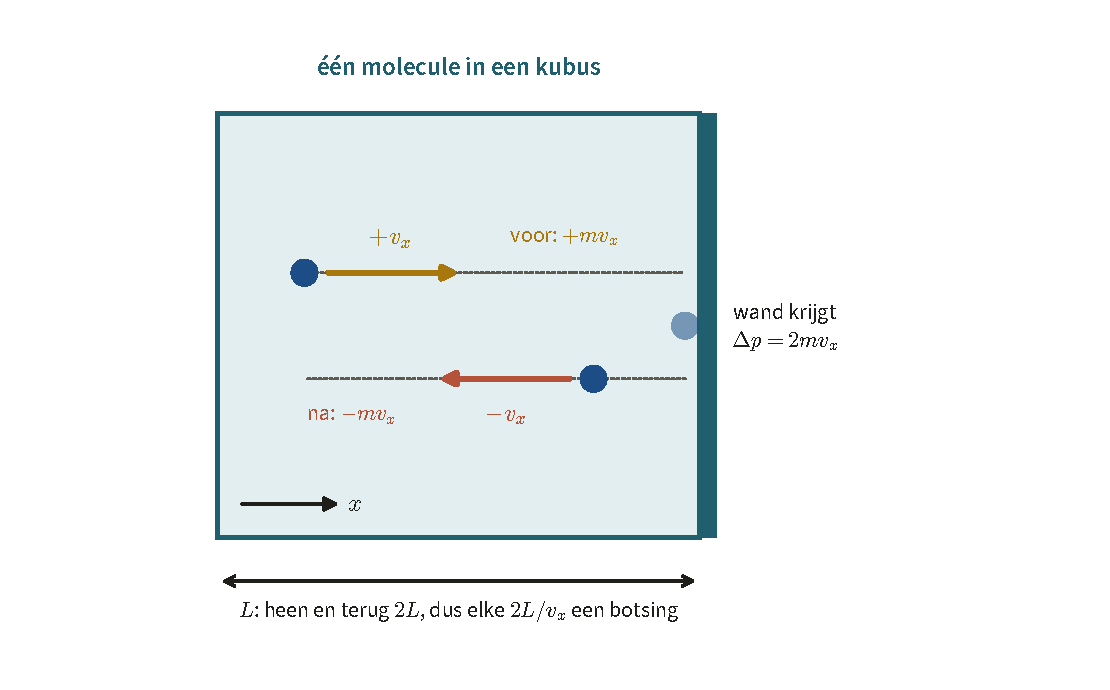
\includegraphics[width=0.85\linewidth]{Figuren/kmt_botsing}
    \caption{\'E\'en molecule in een kubus met ribbe $L$, die in de $x$-richting heen en weer beweegt. Bij elke botsing keert $v_x$ om en krijgt de wand een impuls $2mv_x$; na een heen-en-terugreis $2L$ komt de molecule terug.}
    \label{fig:kmt-botsing}
\end{figure}

\textbf{Stap 1: \'e\'en botsing.} Een molecule met snelheidscomponent $v_x$ botst elastisch tegen de wand loodrecht op $x$. Alleen $v_x$ keert om; $v_y$ en $v_z$ blijven gelijk. De impuls in de $x$-richting gaat van $+mv_x$ naar $-mv_x$, dus de wand krijgt een stoot $2mv_x$.

\textbf{Stap 2: hoe vaak?} Na de botsing moet de molecule naar de overkant en terug, een afstand $2L$. Dat duurt $2L/v_x$, dus ze botst $v_x/(2L)$ keer per seconde tegen dezelfde wand. De gemiddelde kracht van deze ene molecule is stoot maal frequentie:
\[
F_1 = 2mv_x \cdot \frac{v_x}{2L} = \frac{m v_x^2}{L}.
\]
Merk op dat $v_x$ hier \emph{twee keer} meetelt: een snellere molecule botst harder \'en vaker. Daarom verschijnt het kwadraat.

\textbf{Stap 3: alle moleculen samen.} Niet alle moleculen zijn even snel: sommige hebben een grote $v_x$, andere een kleine. We tellen de krachten van alle $N$ moleculen op en delen door de wandoppervlakte $L^2$. Met $L^3 = V$ wordt dat
\[
p = \frac{Nm\langle v_x^2\rangle}{V},
\]
met $\langle v_x^2\rangle$ het gemiddelde van $v_x^2$ over alle moleculen.

\paragraph{Waarom $\langle v^2\rangle$ en niet de gemiddelde snelheid?}
Je zou kunnen proberen te rekenen met \'e\'en ``gemiddelde'' snelheid, maar dat werkt niet. Het gemiddelde van $v_x$ zelf is nul: er bewegen evenveel moleculen naar links als naar rechts. Toch oefenen ze allemaal druk uit, elk op de wand waar ze naartoe vliegen. Wat telt is $v_x^2$, en dat is altijd positief. Het gemiddelde van een kwadraat is bovendien niet het kwadraat van een gemiddelde: wie $\langle v_x^2\rangle$ vervangt door $\langle |v_x|\rangle^2$, onderschat de druk, omdat de snelle moleculen in het kwadraat zwaarder doorwegen.

Rest nog de stap van $v_x$ naar de volledige snelheid. Voor elke molecule is $v^2 = v_x^2 + v_y^2 + v_z^2$ (Pythagoras). In een gas is geen enkele richting bevoordeeld (het gas is \emph{isotroop}), zodat de drie gemiddelden gelijk zijn: $\langle v_x^2\rangle = \langle v_y^2\rangle = \langle v_z^2\rangle = \tfrac{1}{3}\langle v^2\rangle$. Dus
\begin{equation}
pV = \tfrac{1}{3}\,N m \langle v^2\rangle .
\label{eq:kmt-druk}
\end{equation}
Druk is dus niets anders dan het gevolg van ontelbare kleine botsingen tegen de wand.

Vergelijken we dit met $pV = nRT$, dan volgt met $Nm = nM$ (molaire massa $M$):
\begin{equation}
\boxed{\tfrac{1}{2}M\langle v^2\rangle = \tfrac{3}{2}RT}
\qquad\text{of}\qquad
\boxed{v_\mathrm{rms} = \sqrt{\langle v^2\rangle} = \sqrt{\frac{3RT}{M}}}
\label{eq:vrms}
\end{equation}
De wortel uit het gemiddelde kwadraat heet de \emph{rms-snelheid} (root mean square). Ze is iets groter dan de gemiddelde snelheid $\bar v = \sqrt{8RT/\pi M}$, die we in hoofdstuk~\ref{ch:kinetiek} gebruiken voor botsingen tussen moleculen: $\bar v = 0.92\,v_\mathrm{rms}$. Voor de druk en de energie is $v_\mathrm{rms}$ de juiste grootheid, omdat beide met $v^2$ gaan. De temperatuur is dus een rechtstreekse maat voor de gemiddelde kinetische energie van de moleculen: $\tfrac{3}{2}RT$ per mol, of $\tfrac{3}{2}k_\mathrm{B}T$ per molecule. Voor een \'e\'enatomig ideaal gas is dat meteen de volledige interne energie, $U_\mathrm{m} = \tfrac{3}{2}RT$, zodat $C_{V,\mathrm{m}} = \tfrac{3}{2}R$ (zie \S~\ref{sec:warmtecapaciteiten}).

\begin{voorbeeld}{Hoe snel bewegen luchtmoleculen?}
Voor stikstof bij \SI{25}{\celsius} ($M = \SI{0.028}{\kilo\gram\per\mole}$):
\[
v_\mathrm{rms} = \sqrt{\frac{3(8.314)(298)}{0.028}} = \SI{515}{\metre\per\second}.
\]
Dat is sneller dan het geluid (\SI{346}{\metre\per\second}), wat logisch is: geluid wordt doorgegeven door botsende moleculen en kan dus niet sneller gaan dan de moleculen zelf. Helium ($M = \SI{0.004}{\kilo\gram\per\mole}$) is $\sqrt{28/4}\approx 2.6$ keer sneller: \SI{1360}{\metre\per\second}.

Toch ruik je een geopende parfumfles pas na enkele seconden aan de andere kant van de kamer. Een molecule vliegt immers niet rechtdoor: bij atmosferische druk botst ze ongeveer $10^{10}$ keer per seconde met andere moleculen. Botsingen tussen moleculen komen terug in hoofdstuk~\ref{ch:kinetiek}, waar ze de basis vormen van de reactiesnelheid.
\end{voorbeeld}

\begin{toepassing}{Effusie: de wet van Graham}
Wanneer een gas door een zeer klein gaatje ontsnapt (\emph{effusie}), is de snelheid waarmee dat gebeurt evenredig met de molecuulsnelheid, en dus met $1/\sqrt{M}$. Voor twee gassen bij dezelfde $T$ en $p$ geldt de \emph{wet van Graham}:
\begin{equation}
\frac{\text{effusiesnelheid A}}{\text{effusiesnelheid B}} = \sqrt{\frac{M_\mathrm{B}}{M_\mathrm{A}}}.
\end{equation}
\begin{itemize}
\item Een heliumballon loopt sneller leeg dan een luchtballon: helium ontsnapt $\sqrt{29/4}\approx 2.7$ keer sneller door de microporiën van het rubber.
\item Bij de verrijking van uranium wordt het verschil tussen \ce{^{235}UF6} en \ce{^{238}UF6} benut. De verhouding van de effusiesnelheden is slechts $\sqrt{352.0/349.0} = 1.0043$. Daarom waren duizenden diffusietrappen achter elkaar nodig; vandaag gebruikt men gascentrifuges.
\item Lekdetectie in vacu\"umsystemen gebeurt met helium: het lichte, snelle heliumatoom vindt zelfs de kleinste lekken.
\end{itemize}
\end{toepassing}

\subsection{Afwijkingen van ideaal gedrag}

Bij hoge druk en lage temperatuur gaan aannames (2) en (3) niet meer op. Dat zie je op drie manieren.
\begin{itemize}
\item \textbf{$pV$ is niet constant.} Volgens Boyle is $pV$ bij constante $T$ onafhankelijk van de druk (figuur~\ref{fig:Boyle}, links). Vergelijk je beide panelen van figuur~\ref{fig:Boyle}, dan zie je hoe groot de afwijking voor \ce{CO2} wordt: bij \SI{20}{\celsius} en \SI{0.5}{\litre\per\mole} voorspelt de ideale gaswet \SI{48.7}{\bar}, terwijl de werkelijke druk ongeveer \SI{37}{\bar} is, bijna een kwart lager. Voor een gas als stikstof bij kamertemperatuur blijft de afwijking onder \SI{10}{\bar} kleiner dan \SI{1}{\percent}, maar bij enkele honderden bar loopt ze op tot tientallen procenten.
\item \textbf{Joule--Thomson-effect.} Een gas dat zonder warmte-uitwisseling door een ventiel expandeert, koelt bij kamertemperatuur meestal af. Bij een ideaal gas zou $T$ constant blijven. De interne energie van een re\"eel gas hangt dus af van het volume: de moleculen trekken elkaar aan.
\item \textbf{Condensatie.} Volgens de ideale gaswet kan je een gas tot een willekeurig klein volume samenpersen. In werkelijkheid condenseert elk gas onder zijn \emph{kritische temperatuur} $T_c$ tot een vloeistof met een nagenoeg vast volume (figuur~\ref{fig:Boyle}, rechts). Boven $T_c$ (voor \ce{CO2} \SI{31.0}{\celsius}) condenseert het nooit, hoe hoog de druk ook wordt.
\end{itemize}

\begin{figure}[htb]
    \centering
    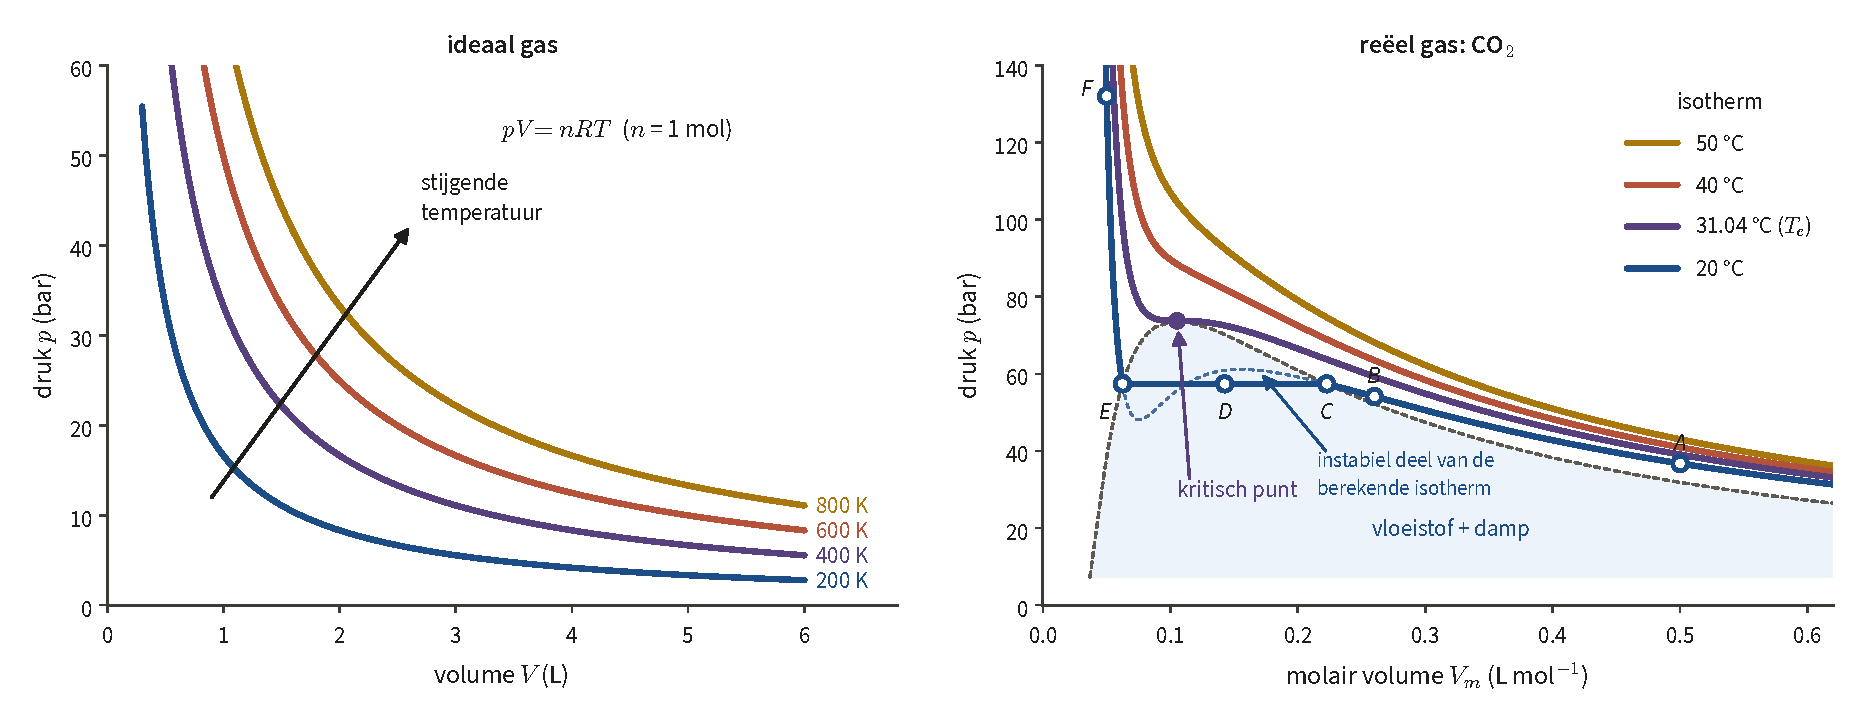
\includegraphics[width=\linewidth]{Figuren/isothermen_vergelijking}
    \caption{Isothermen van \ce{CO2} bij dezelfde temperaturen en op dezelfde assen. Links berekend met de ideale gaswet: $p \propto 1/V_m$ over het volledige bereik. Rechts het werkelijke gedrag (berekend met de toestandsvergelijking van Peng--Robinson, \S~\ref{sec:andere-toestandsvgl}). Bij groot molair volume liggen beide dicht bij elkaar; bij kleiner volume ligt de werkelijke druk lager. Onder de kritische temperatuur verschijnt een horizontaal stuk (C $\to$ E): daar condenseert het gas bij constante druk.}
    \label{fig:Boyle}
\end{figure}

\subsection{De vergelijking van Van der Waals}
\label{sec:vdw-afleiding}

Aannames (2) en (3) uit de ideale gaswet zijn niet exact: moleculen hebben wel een eigen volume en trekken elkaar wel aan. In 1873 corrigeerde Johannes Diderik van der Waals de ideale gaswet voor beide effecten, niet met een empirische fit maar vanuit hun fysische oorsprong. Hij verkreeg hiervoor de  Nobelprijs in 1910. Hieronder bespreken we zijn redenering in drie stappen.

\subsubsection{Stap 1: het uitgesloten volume}

\begin{figure}[htb]
    \centering
    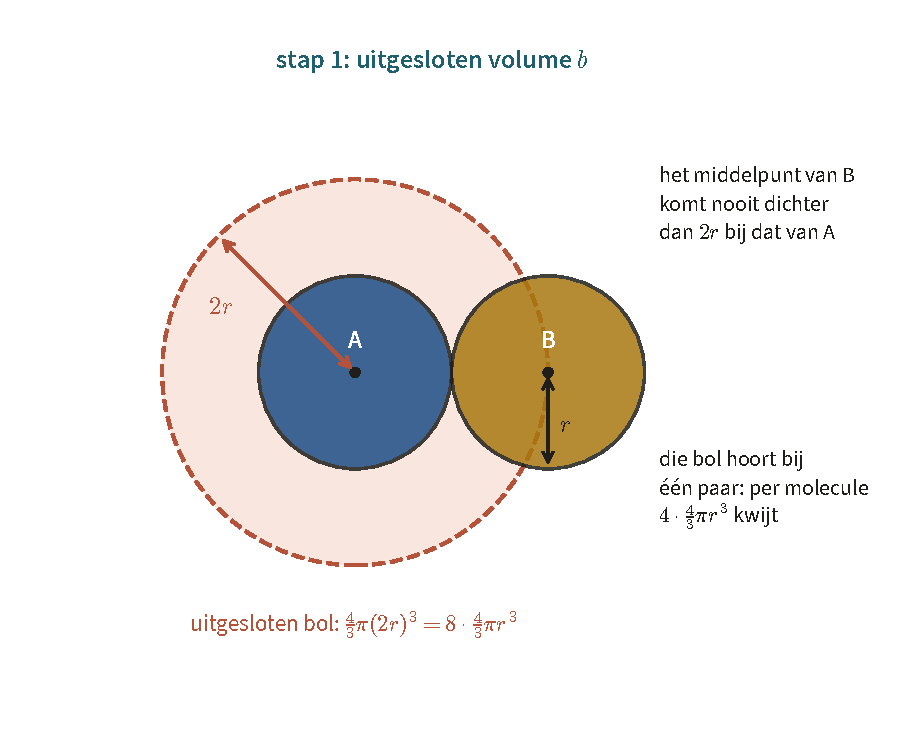
\includegraphics[width=0.6\linewidth]{Figuren/vdw_uitgesloten}
    \caption{Het uitgesloten volume. Rond molecule A ligt een bol met straal $2r$ waarin het middelpunt van B niet kan komen; dat volume is niet beschikbaar voor de beweging.}
    \label{fig:vdw-uitgesloten}
\end{figure}

Moleculen zijn geen puntmassa's (figuur~\ref{fig:vdw-uitgesloten}). Twee harde bollen met straal $r$ kunnen elkaars middelpunt niet dichter naderen dan $2r$. Rond elke molecule ligt dus een uitgesloten bol met volume $\tfrac{4}{3}\pi(2r)^3 = 8\cdot\tfrac{4}{3}\pi r^3$. Die bol is geen eigenschap van A alleen, maar van het paar A--B: hij beschrijft hoe dicht die twee elkaar kunnen naderen. Per molecule rekenen we hem dus maar half aan, zodat per molecule $4\cdot\tfrac{4}{3}\pi r^3$ is uitgesloten. Per mol is dat het \emph{co-volume} gelijk aan:
\begin{equation*}
b = 4 N_\mathrm{A} \cdot \tfrac{4}{3}\pi r^3 
\end{equation*}
Dit is viermaal het eigenlijke volume van de moleculen. Hierdoor is het vrije volume in de ruimte gelijk aan $V - nb$, en dus
\begin{equation}
p(V - nb) = nRT.
\end{equation}


\subsubsection{Stap 2: de drukcorrectie - intermoleculaire aantrekkingskrachten}

\begin{figure}[htb]
    \centering
    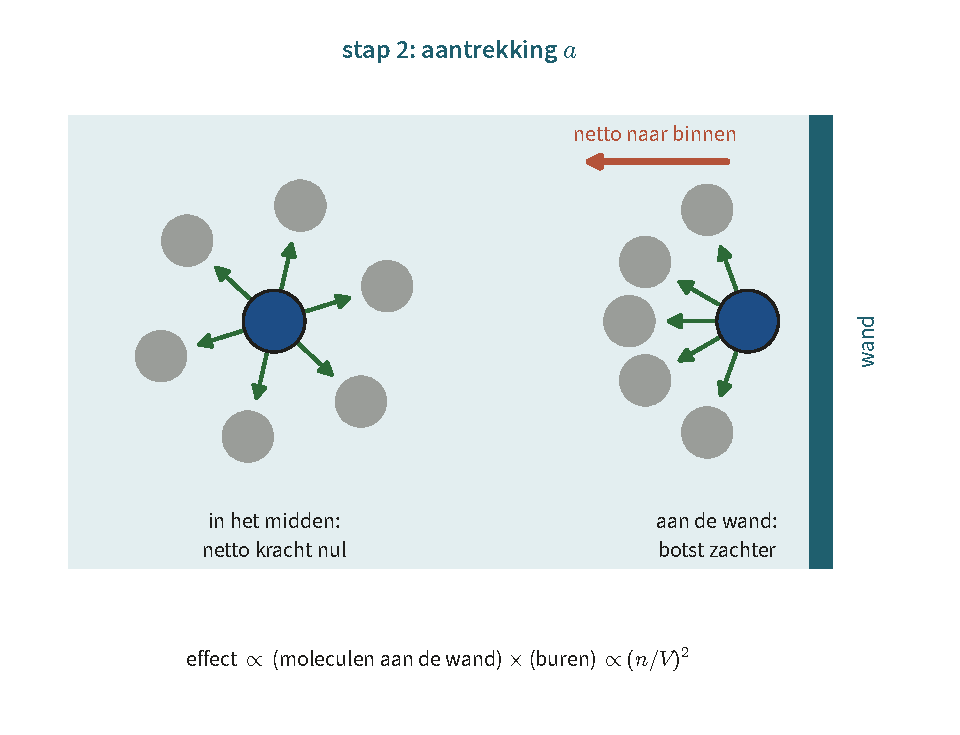
\includegraphics[width=0.65\linewidth]{Figuren/vdw_aantrekking}
    \caption{De aantrekking tussen moleculen. Een molecule in het midden van het gas wordt in alle richtingen even sterk aangetrokken, een molecule aan de wand enkel naar binnen. Ze botst daardoor zachter tegen de wand.}
    \label{fig:vdw-aantrekking}
\end{figure}

Reële moleculen trekken elkaar bovendien aan (figuur~\ref{fig:vdw-aantrekking}). Midden in het gas is een molecule langs alle kanten omringd door buren; hun aantrekkingskrachten heffen elkaar gemiddeld op. Een molecule die de wand nadert, heeft echter enkel nog buren aan de binnenkant en wordt dus netto teruggetrokken. Ze botst daardoor met een kleinere impuls tegen de wand, en de gemeten druk is lager dan bij een ideaal gas. Van der Waals schreef daarom
\begin{equation*}
p_{\mathrm{ideaal}} = p + p_{\mathrm{correctie}}.
\end{equation*}
Die correctie hangt af van het aantal paren moleculen dat elkaar aantrekt. Zowel het aantal moleculen nabij de wand als het aantal buren dat aan elk ervan trekt, is evenredig met de dichtheid $n/V$. De correctie is dus evenredig met het kwadraat: verdubbel je de dichtheid, dan wordt het effect vier keer groter.
\begin{equation}
p_{\mathrm{correctie}} = a\frac{n^2}{V^2}
\end{equation}
De stofconstante $a$ meet de sterkte van de aantrekking: groot voor \ce{CO2} en \ce{NH3}, klein voor He en \ce{H2}.

\subsubsection{Stap 3: combinatie van beide correcties}

Vervang in de ideale gaswet $p_{\mathrm{ideaal}} \to p + a n^2/V^2$ en $V_{\mathrm{ideaal}} \to V - nb$:
\begin{equation}
\boxed{\;\left(p + \frac{a n^2}{V^2}\right)(V - nb) = nRT\;}
\qquad\text{of per mol}\qquad
\boxed{\;\left(p + \frac{a}{V_m^2}\right)(V_m - b) = RT\;}
\label{eq:vdw}
\end{equation}

De parameters $a$ en $b$ zijn stofconstanten: je hoeft ze niet zelf te bepalen, maar zoekt ze op in tabellen. Tabel~\ref{tab:vdw-kort} geeft ze voor enkele veelgebruikte gassen; tabel~\ref{tab:kritiek} in bijlage~\ref{ch:tabellen} bevat een uitgebreidere lijst. De waarden tonen het fysische beeld van hierboven: kleine, apolaire moleculen (He, \ce{H2}) hebben een kleine $a$, polaire moleculen (\ce{NH3}, \ce{H2O}) en grotere moleculen (\ce{CO2}) een grote. De parameter $b$ volgt de grootte van de molecule.

\begin{table}[htb]
\centering
\caption{Van der Waals-parameters van enkele gassen, berekend uit de kritieke constanten met vergelijking~\eqref{eq:vdw-ab}. Bron kritieke constanten: zie tabel~\ref{tab:kritiek}.}
\label{tab:vdw-kort}
\begin{tabular}{lcc}
\toprule
gas & $a$ (\si{\pascal\metre\tothe{6}\per\mole\squared}) & $b$ ($10^{-5}$ \si{\metre\cubed\per\mole}) \\
\midrule
He & 0.0035 & 2.38 \\
\ce{H2} & 0.0248 & 2.66 \\
\ce{N2} & 0.137 & 3.86 \\
\ce{CH4} & 0.230 & 4.31 \\
\ce{CO2} & 0.366 & 4.29 \\
\ce{NH3} & 0.425 & 3.74 \\
\ce{H2O} & 0.553 & 3.05 \\
\bottomrule
\end{tabular}
\end{table}

\subsubsection{Het kritiek punt}

Een groot succes van de vergelijking is dat ze het \emph{kritiek punt} voorspelt. Wat is dat precies? Verwarm een vloeistof met haar damp in een gesloten, stevig vat. De vloeistof zet uit en wordt minder dicht; tegelijk verdampt er meer, zodat de damp erboven dichter wordt. Bij een bepaalde temperatuur worden beide dichtheden gelijk. Het scheidingsvlak (de meniscus) verdwijnt, en er is nog maar \'e\'en homogene fase. Die temperatuur is de \emph{kritieke temperatuur} $T_c$, de bijbehorende druk de \emph{kritieke druk} $p_c$ en het molair volume het \emph{kritieke volume} $V_{m,c}$.

Daaruit volgen twee praktische gevolgen:
\begin{itemize}
\item Boven $T_c$ kan je een gas \emph{niet} meer vloeibaar maken, hoe hoog je de druk ook opdrijft. Wie een gas wil vloeibaar maken (\ce{N2} of aardgas), moet het dus eerst onder $T_c$ afkoelen: voor stikstof onder \SI{126}{\kelvin}.
\item Boven $T_c$ \'en $p_c$ spreken we van een \emph{superkritisch fluïdum}. Het is zo dicht als een vloeistof en lost dus goed op, maar het stroomt en diffundeert als een gas. Superkritisch \ce{CO2} ($T_c = \SI{31}{\celsius}$, $p_c = \SI{74}{\bar}$) wordt zo gebruikt om cafe\"ine uit koffiebonen te extraheren, zonder resten van organische solventen.
\end{itemize}

Figuur~\ref{fig:vdw-isothermen} toont hoe de vergelijking van Van der Waals dit weergeeft. Boven $T_c$ daalt de druk monotoon met het volume: er is maar \'e\'en fase. Onder $T_c$ vertoont de isotherm een S-vormige lus. In werkelijkheid volgt het systeem die lus niet: het gas condenseert bij constante druk, langs het horizontale stuk (vergelijk met figuur~\ref{fig:Boyle}, rechts). Alle horizontale stukken samen vormen het tweefasengebied. Het kritiek punt is de top ervan: de isotherm bij $T_c$ is daar net horizontaal \'en verandert van kromming. Wiskundig is het dus een buigpunt met horizontale raaklijn:
\begin{equation*}
\left.\frac{\partial p}{\partial V_m}\right|_{T_c} = -\frac{RT_c}{(V_{m,c} - b)^2} + \frac{2a}{V_{m,c}^3} = 0,
\qquad
\left.\frac{\partial^2 p}{\partial V_m^2}\right|_{T_c} = \frac{2RT_c}{(V_{m,c} - b)^3} - \frac{6a}{V_{m,c}^4} = 0.
\end{equation*}

\begin{figure}[htb]
    \centering
    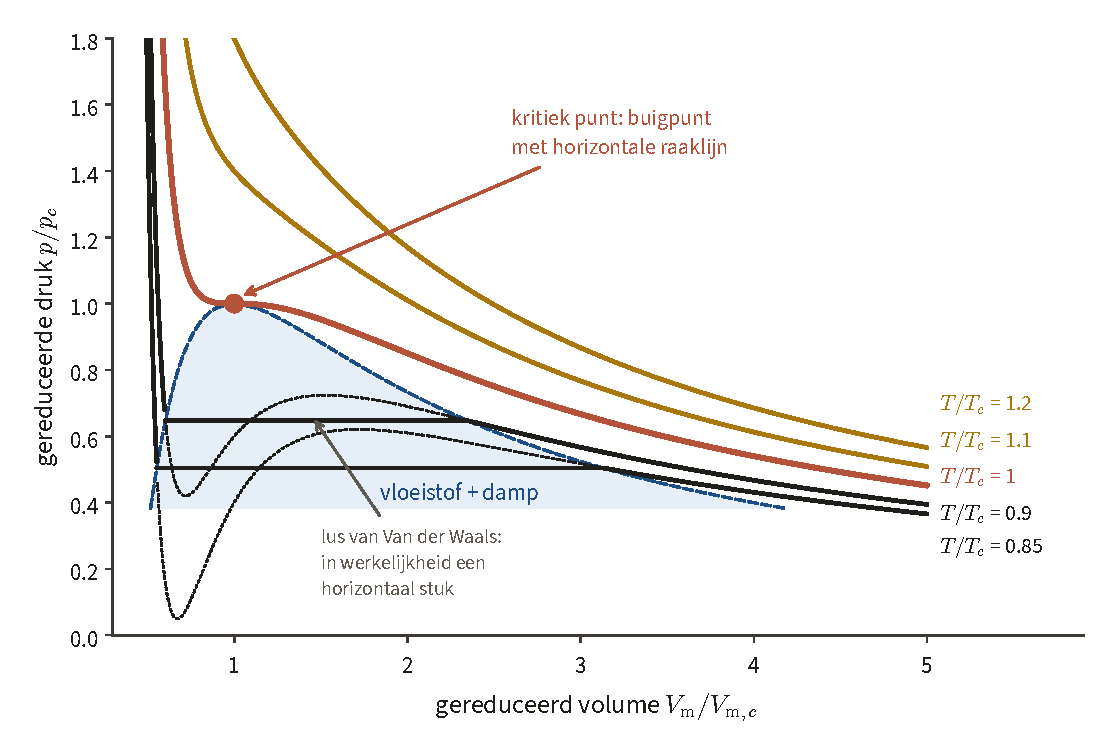
\includegraphics[width=0.85\linewidth]{Figuren/vdw_isothermen}
    \caption{Isothermen van Van der Waals in gereduceerde vorm ($p/p_c$ tegen $V_m/V_{m,c}$). Boven $T_c$ is er \'e\'en fase. Onder $T_c$ wordt de lus (stippellijn) in werkelijkheid vervangen door een horizontaal stuk: het gas condenseert bij constante druk. Het gekleurde gebied is het tweefasengebied, het kritiek punt de top ervan.}
    \label{fig:vdw-isothermen}
\end{figure}
Samen met de vergelijking zelf levert dit
\begin{equation}
V_{m,c} = 3b, \qquad T_c = \frac{8a}{27Rb}, \qquad p_c = \frac{a}{27b^2}
\qquad\Longleftrightarrow\qquad
a = \frac{27 R^2 T_c^2}{64 p_c}, \qquad b = \frac{R T_c}{8 p_c}.
\label{eq:vdw-ab}
\end{equation}
Zo bepaalt men $a$ en $b$ ook in de praktijk: de kritieke temperatuur en druk zijn nauwkeurig meetbaar, en daaruit volgen de parameters.

\begin{voorbeeld}{$a$ en $b$ voor $\mathrm{CO_2}$ uit het kritiek punt}
Met $T_c = \SI{304.2}{\kelvin}$ en $p_c = \SI{73.8}{\bar}$ (tabel~\ref{tab:kritiek}):
\begin{align*}
a &= \frac{27(8.314)^2(304.2)^2}{64(7.38\times10^{6})} = \SI{0.366}{\pascal\metre\tothe{6}\per\mole\squared},\\
b &= \frac{(8.314)(304.2)}{8(7.38\times10^{6})} = \SI{4.29e-5}{\metre\cubed\per\mole}.
\end{align*}
Dit zijn precies de waarden van tabel~\ref{tab:vdw-kort}: zo zijn die tabelwaarden ook berekend.
\end{voorbeeld}

\subsection{De compressibiliteitsfactor}

De afwijking wordt gemeten met de \emph{compressibiliteitsfactor}
\begin{equation}
\boxed{\;Z = \frac{V_\mathrm{m}}{V_\mathrm{m}^\text{ideaal}} = \frac{pV_\mathrm{m}}{RT}\;}
\end{equation}
Voor een ideaal gas is $Z = 1$. Bij $Z < 1$ is het gas compacter dan ideaal: de \emph{aantrekking} tussen de moleculen domineert (matige druk, lage $T$). Bij $Z > 1$ is het gas minder samendrukbaar: het \emph{eigen volume} van de moleculen domineert (zeer hoge druk). Voor $p \to 0$ of $T \to \infty$ gaat $Z \to 1$. Tabel~\ref{table:Z} en figuur~\ref{fig:Z} tonen dat verloop.

\begin{table}[htb]
\centering
\caption{Compressibiliteitsfactor $Z$ voor \ce{CO2} bij \SI{350}{\kelvin}.}
\label{table:Z}
\begin{tabular}{ccc}
\toprule
$p$ (\si{\bar}) & $V_\mathrm{m}$ (\si{\litre\per\mole}) & $Z$ \\
\midrule
1 & 24.5 & 1.00 \\
50 & 0.41 & 0.70 \\
200 & 0.15 & 1.03 \\
1000 & 0.045 & 2.16 \\
\bottomrule
\end{tabular}
\end{table}

\begin{figure}[htb]
    \centering
    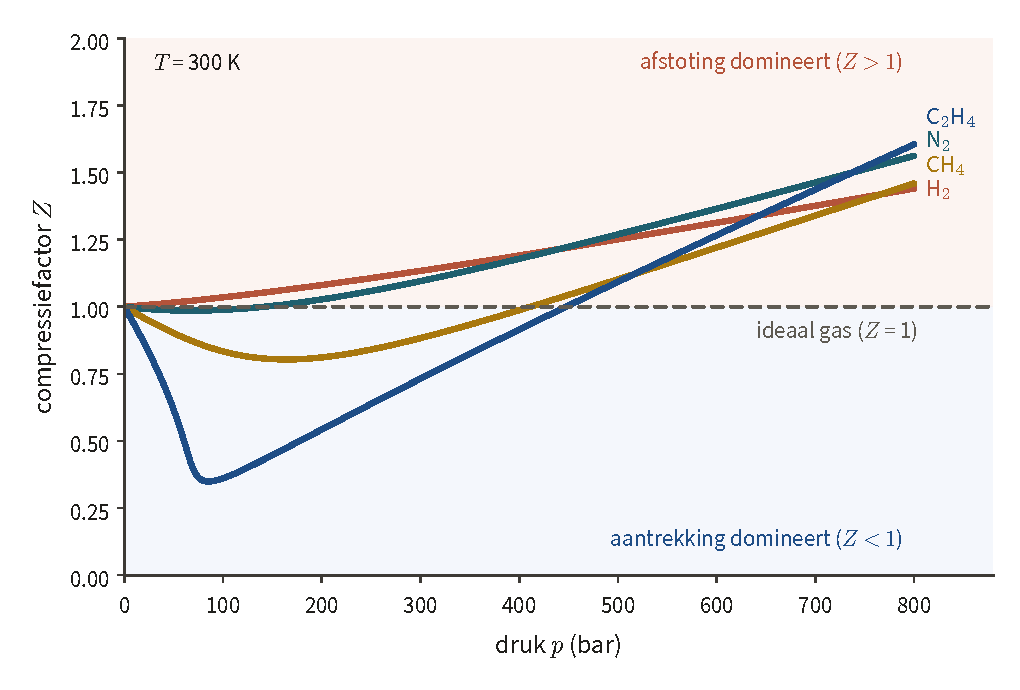
\includegraphics[width=0.7\linewidth]{Figuren/compressiefactor}
    \caption{Compressibiliteitsfactor in functie van de druk. Bij lage druk domineert de aantrekking ($Z<1$), bij hoge druk het eigen volume ($Z>1$).}
    \label{fig:Z}
\end{figure}

De vergelijking van Van der Waals verklaart beide richtingen. Je berekent $Z$ door eerst de druk uit vergelijking~\eqref{eq:vdw} te halen en die dan in de definitie van $Z$ in te vullen.

\begin{voorbeeld}{Vergelijking van het gedrag van \ce{CO2} en He}
We vergelijken beide gassen bij $T = \SI{300}{\kelvin}$ en $V_m = \SI{1.00e-3}{\metre\cubed\per\mole}$ (\SI{1.00}{\litre\per\mole}). De parameters $a$ en $b$ komen uit tabel~\ref{tab:vdw-kort}. Herschreven naar $p$ luidt de vergelijking van Van der Waals
\[
p = \frac{RT}{V_m - b} - \frac{a}{V_m^2},
\qquad\text{met}\qquad RT = (8.314)(300) = \SI{2494}{\joule\per\mole}.
\]
\textbf{Ideaal gas.} $p = RT/V_m = 2494/(1.00\times10^{-3}) = \SI{2.49}{\mega\pascal}$, en per definitie $Z = 1$.

\textbf{\ce{CO2}} ($a = \SI{0.366}{\pascal\metre\tothe{6}\per\mole\squared}$, $b = \SI{4.29e-5}{\metre\cubed\per\mole}$):
\begin{align*}
p &= \frac{2494}{1.00\times10^{-3} - 0.0429\times10^{-3}} - \frac{0.366}{(1.00\times10^{-3})^2}
   = \frac{2494}{0.957\times10^{-3}} - 0.366\times10^{6}\\
  &= 2.606\times10^{6} - 0.366\times10^{6} = \SI{2.24e6}{\pascal},\\
Z &= \frac{pV_m}{RT} = \frac{(2.24\times10^{6})(1.00\times10^{-3})}{2494} = 0.898.
\end{align*}
\textbf{He} ($a = \SI{0.0035}{\pascal\metre\tothe{6}\per\mole\squared}$, $b = \SI{2.38e-5}{\metre\cubed\per\mole}$):
\begin{align*}
p &= \frac{2494}{0.976\times10^{-3}} - \frac{0.0035}{(1.00\times10^{-3})^2}
   = 2.555\times10^{6} - 0.0035\times10^{6} = \SI{2.55e6}{\pascal},\\
Z &= \frac{(2.55\times10^{6})(1.00\times10^{-3})}{2494} = 1.023.
\end{align*}
Beide gassen wijken in tegengestelde richting af. Bij \ce{CO2} is de aantrekkingsterm groot ($a/V_m^2$ is ongeveer \SI{15}{\percent} van de druk): de aantrekking wint en $Z < 1$. Bij helium is de aantrekking verwaarloosbaar en verhoogt alleen het eigen volume de druk: $Z > 1$.
\end{voorbeeld}

Ook in het kritiek punt kan je $Z$ berekenen. Van der Waals voorspelt voor elk gas dezelfde waarde: met $V_{m,c} = 3b$, $T_c = 8a/(27Rb)$ en $p_c = a/(27b^2)$ volgt
\[
Z_c = \frac{p_c V_{m,c}}{RT_c} = \frac{3}{8} = 0.375.
\]
Gemeten waarden liggen lager en verschillen van stof tot stof: 0.301 (He), 0.290 (\ce{N2}), 0.274 (\ce{CO2}), 0.242 (\ce{NH3}) en 0.229 (\ce{H2O}) (tabel~\ref{tab:kritiek}). Van der Waals is dus kwalitatief juist, maar kwantitatief beperkt, vooral voor polaire stoffen.

Zet je $Z$ uit tegen de \emph{gereduceerde druk} $p_r = p/p_c$ bij een vaste \emph{gereduceerde temperatuur} $T_r = T/T_c$, dan vallen de curves van heel verschillende gassen nagenoeg samen (figuur~\ref{fig:compchart}). Dit is de \emph{wet van de corresponderende toestanden}. Ingenieurs gebruiken zulke algemene compressibiliteitskaarten wanneer geen specifieke toestandsvergelijking beschikbaar is.

\begin{figure}[htb]
    \centering
    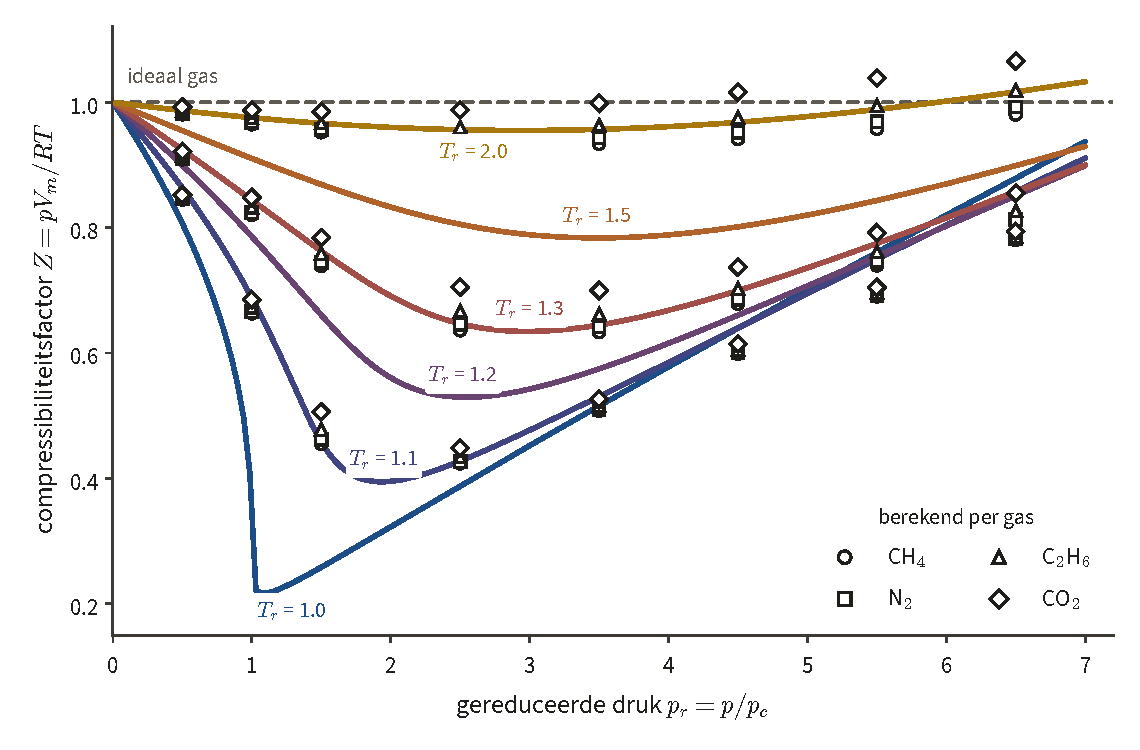
\includegraphics[width=0.7\linewidth]{Figuren/compressibiliteitskaart}
    \caption{Algemene compressibiliteitskaart: $Z$ tegen $p_r$ voor verschillende gassen bij dezelfde $T_r$.}
    \label{fig:compchart}
\end{figure}

\subsection{Andere toestandsvergelijkingen}
\label{sec:andere-toestandsvgl}

De vergelijking van Van der Waals schiet om drie redenen tekort: moleculen zijn geen harde bollen, de aantrekking $a$ hangt in werkelijkheid van de temperatuur af, en vloeistofdichtheden worden slecht voorspeld. Voor nauwkeurig ontwerpwerk gebruiken ingenieurs daarom andere toestandsvergelijkingen. Er zijn twee families.

\subsubsection{Kubische toestandsvergelijkingen}

Deze vergelijkingen behouden de structuur van Van der Waals, een afstotingsterm min een aantrekkingsterm, maar verfijnen beide. De belangrijkste zijn
\begin{align*}
\text{Redlich--Kwong (1949):}\quad & p = \frac{RT}{V_m - b} - \frac{a}{\sqrt{T}\,V_m(V_m + b)},\\
\text{Peng--Robinson (1976):}\quad & p = \frac{RT}{V_m - b} - \frac{a\,\alpha(T)}{V_m(V_m + b) + b(V_m - b)}.
\end{align*}
Soave--Redlich--Kwong (1972) vervangt in Redlich--Kwong de factor $1/\sqrt{T}$ door een functie $\alpha(T)$, zoals ook Peng--Robinson doet. Die $\alpha(T)$ hangt af van de \emph{acentrische factor} $\omega$, een getal uit tabellen dat meet hoe sterk een stof afwijkt van een eenvoudige, bolvormige molecule zoals argon. De parameters $a$ en $b$ volgen, net als bij Van der Waals, uit $T_c$ en $p_c$.

Ze heten \emph{kubisch} omdat ze, uitgewerkt naar $V_m$, een derdegraadsvergelijking opleveren. Onder de kritieke temperatuur ($T_c$) zijn die drie wortels: de kleinste is het molair volume van de vloeistof, de grootste dat van de damp, de middelste heeft geen fysische betekenis. Zo beschrijft \'e\'en vergelijking zowel de toestand van de gas- als vloeistoffase. Soave--Redlich--Kwong en Peng--Robinson zijn de standaard in processimulatoren zoals Aspen Plus en HYSYS; ook figuur~\ref{fig:Z} is met Peng--Robinson berekend.

\subsubsection{De viriaalvergelijking}

Een heel andere aanpak schrijft de afwijking van het ideaal gas als een machtreeks in $1/V_m$:
\begin{equation}
Z = \frac{pV_m}{RT} = 1 + \frac{B(T)}{V_m} + \frac{C(T)}{V_m^2} + \dots
\label{eq:viriaal}
\end{equation}
$B$ en $C$ heten de tweede en derde \emph{viriaalco\"effici\"ent}. Ze hangen enkel van de temperatuur af en worden per stof bepaald door de reeks te fitten op gemeten $p$-$V$-$T$-gegevens (tabel~\ref{tab:viriaal}).

\begin{table}[htb]
\centering
\caption{Tweede viriaalco\"effici\"ent $B$ (\si{\centi\metre\cubed\per\mole}).}
\label{tab:viriaal}
\begin{tabular}{lcc}
\toprule
gas & \SI{273}{\kelvin} & \SI{600}{\kelvin} \\
\midrule
He & 12.0 & 10.4 \\
\ce{N2} & $-10.5$ & 21.7 \\
Ar & $-21.7$ & 11.9 \\
\ce{CO2} & $-149.7$ & $-12.4$ \\
\bottomrule
\end{tabular}
\end{table}

Het teken van $B$ vertelt wat domineert. Een negatieve $B$ (\ce{CO2}, en \ce{N2} bij \SI{273}{\kelvin}) betekent $Z < 1$: de aantrekking wint. Bij hogere temperatuur wordt $B$ positief, omdat de moleculen dan zo snel bewegen dat de aantrekking weinig uitmaakt en enkel het eigen volume overblijft. De temperatuur waarbij $B = 0$ heet de \emph{Boyle-temperatuur}: daar gedraagt het gas zich bij lage druk opvallend ideaal.

De viriaalvergelijking is vooral een \emph{fitvergelijking}. Ze vertrekt niet van een fysisch beeld van de moleculen zoals Van der Waals, en de co\"effici\"enten volgen niet uit een theorie maar uit metingen. Dat is meteen haar sterkte: met genoeg termen beschrijft ze experimentele gegevens zo nauwkeurig als je wil. Bij lage tot matige dichtheid volstaat vaak de term in $B$ alleen. Haar zwakte is dat ze enkel geldt in het gebied waarop gefit werd: bij hoge dichtheid en in de buurt van condensatie convergeert de reeks niet meer, en een vloeistof beschrijft ze niet.

\section{Warmte en arbeid}

Tijdens compressie, expansie, opwarming of afkoeling wisselt een systeem energie uit met zijn omgeving. Dat kan op twee manieren: als \emph{arbeid} of als \emph{warmte}. Beide zijn padfuncties, maar ze verschillen fundamenteel van aard (figuur~\ref{fig:arbeid-warmte}).

\begin{figure}[htb]
    \centering
    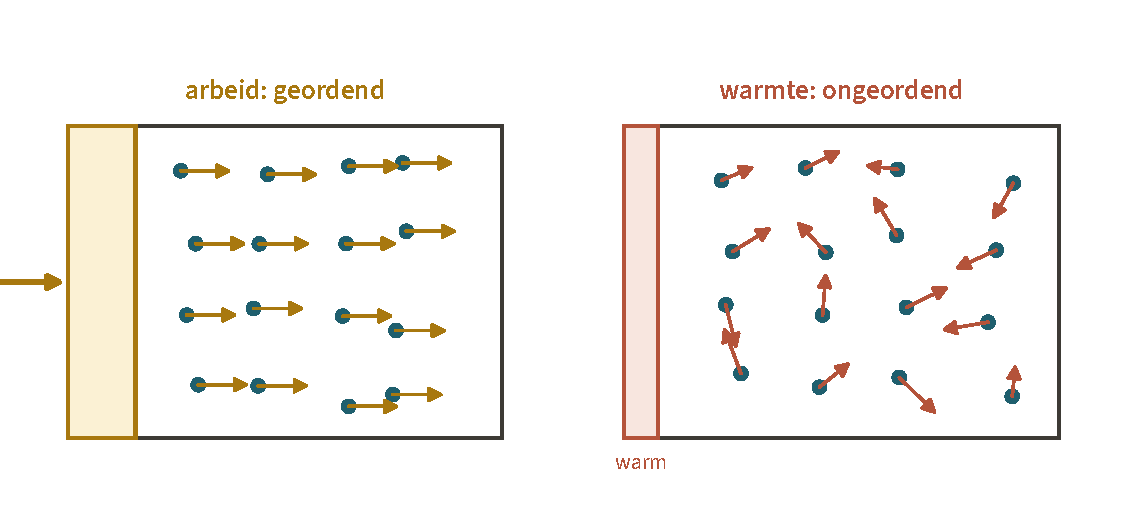
\includegraphics[width=0.85\linewidth]{Figuren/arbeid_warmte}
    \caption{Arbeid is geordende energieoverdracht: de zuiger geeft alle moleculen die hij raakt een duw in dezelfde richting. Warmte is ongeordend: een warme wand geeft moleculen een extra snelheid in willekeurige richtingen.}
    \label{fig:arbeid-warmte}
\end{figure}

\emph{Arbeid} is energieoverdracht door een macroscopische, gerichte kracht: een zuiger die een gas samendrukt, een gewicht dat wordt opgetild, elektronen die samen door een draad bewegen. Arbeid kan in principe volledig worden omgezet in een andere vorm van geordende energie. 

\emph{Warmte} is energieoverdracht die enkel door een temperatuurverschil wordt gedreven. De snelle moleculen van een warme wand stoten tegen de tragere gasmoleculen, die daarna in willekeurige richtingen sneller bewegen. Die wanorde maakt dat warmte niet volledig in arbeid kan worden omgezet; dat is het onderwerp van hoofdstuk~\ref{ch:spontaniteit}.

In chemische processen is de belangrijkste vorm van arbeid de \emph{volumearbeid}, verricht wanneer het volume verandert tegen een uitwendige druk:
\begin{equation}
\boxed{\;\delta W = -p_{\text{ext}}\,\dd V\;}
\end{equation}
We beschouwen energie die het systeem \emph{ontvangt} als positief. Bij expansie ($\dd V > 0$) levert het gas arbeid aan de omgeving, dus $W < 0$. In een $pV$-diagram is $|W|$ de oppervlakte onder de curve (figuur~\ref{fig:padfunctie}).

\begin{voorbeeld}{Arbeid bij isotherme expansie van een ideaal gas}
\SI{1}{\mole} ideaal gas expandeert reversibel en isotherm bij \SI{300}{\kelvin} van \SI{1}{\litre} naar \SI{10}{\litre}. Reversibel betekent $p_\text{ext} = p = nRT/V$, zodat
\[
W = -\int_{V_1}^{V_2} \frac{nRT}{V}\,\dd V = -nRT \ln\frac{V_2}{V_1} = -(1)(8.314)(300)\ln 10 = -\SI{5.74}{\kilo\joule}.
\]
Het gas levert \SI{5.74}{\kilo\joule} arbeid. Laat je het gas in \'e\'en ruk expanderen tegen de constante einddruk $p_\text{ext} = nRT/V_2 = \SI{2.49}{\bar}$, dan is $W = -p_\text{ext}\Delta V = -(2.49\times10^{5})(0.009) = -\SI{2.24}{\kilo\joule}$. Zelfde begin- en eindtoestand, minder dan de helft van de arbeid: arbeid hangt af van de weg.

Figuur~\ref{fig:arbeid-weg} maakt dat zichtbaar. De arbeid is de oppervlakte onder de weg in het $pV$-diagram. Bij de reversibele expansie volgt de uitwendige druk de gasdruk langs de isotherm, en die oppervlakte is groot. In \'e\'en ruk valt de uitwendige druk meteen naar $p_2$, en het gas duwt de hele weg tegen die lage druk: de oppervlakte is enkel de rechthoek onder $p_2$.

\begin{figure}[H]
    \centering
    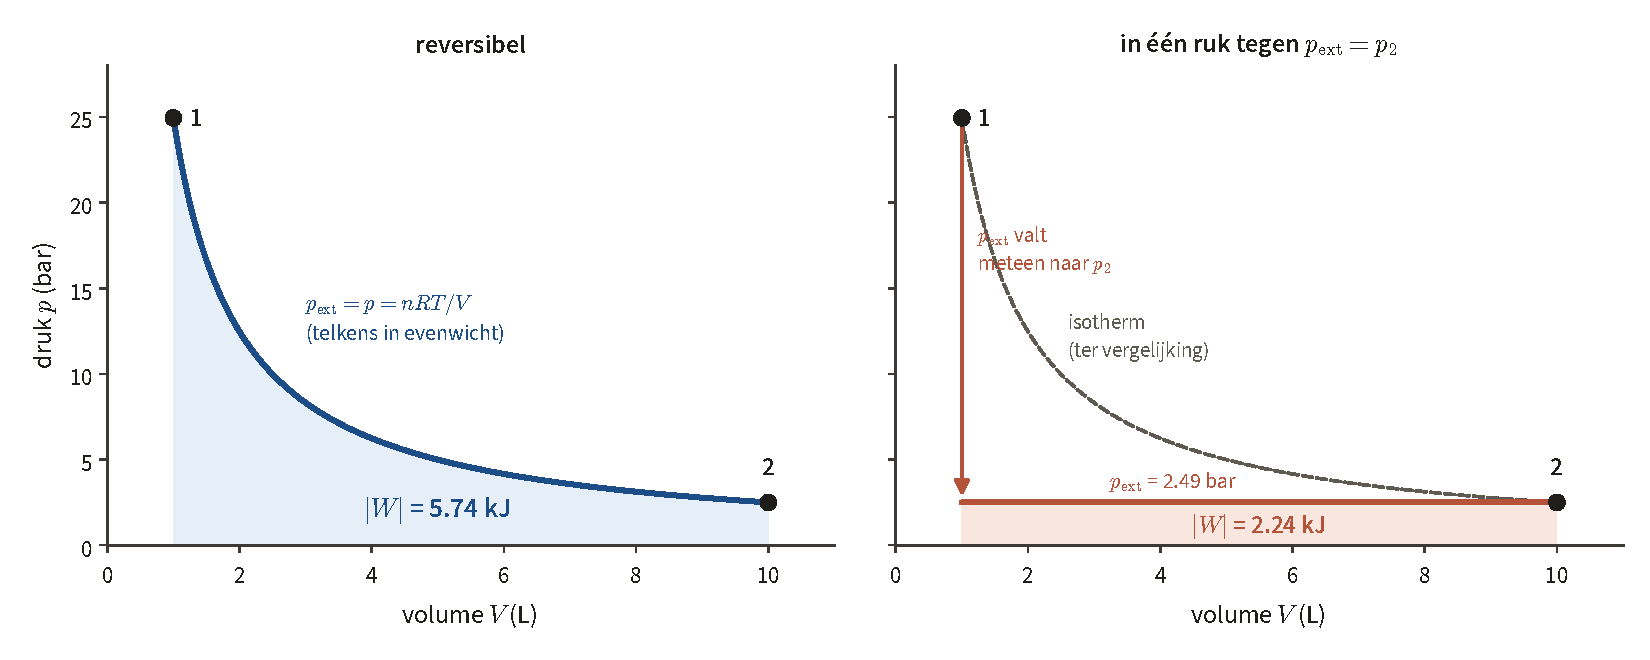
\includegraphics[width=\linewidth]{Figuren/arbeid_weg}
    \caption{Isotherme expansie van \SI{1}{\mole} ideaal gas van \SI{1}{\litre} naar \SI{10}{\litre} bij \SI{300}{\kelvin}. Links reversibel, rechts in \'e\'en ruk tegen $p_\text{ext} = p_2$. De gekleurde oppervlakte is $|W|$.}
    \label{fig:arbeid-weg}
\end{figure}

\textbf{Hoe doe je dit in de praktijk?} De reversibele isotherme expansie van links vraagt twee dingen tegelijk.
\begin{itemize}
\item \emph{Reversibel:} de uitwendige druk mag op elk ogenblik maar een fractie lager zijn dan de gasdruk. Het klassieke gedachte-experiment: belast een wrijvingsloze zuiger met een hoopje fijn zand en neem de korrels er \'e\'en voor \'e\'en af. Elke stap is een kleine expansie; hoe kleiner de stappen, hoe dichter de weg bij de isotherm ligt en hoe meer arbeid het gas levert.
\item \emph{Isotherm:} een gas dat arbeid levert, koelt af: het omgekeerde van de compressor die opwarmt (\S~\ref{sec:compressor}). Om $T$ constant te houden moet de omgeving tijdens de expansie warmte toevoeren, hier $Q = -W = \SI{5.74}{\kilo\joule}$. Dat lukt met een cilinder met dunne, goed geleidende wand in een groot thermostaatbad op \SI{300}{\kelvin}, en door zo traag te werken dat de warmte telkens kan bijbenen.
\end{itemize}
De vuistregel is dus: een proces is (bijna) isotherm als het veel trager verloopt dan de tijd die warmte nodig heeft om het gas te bereiken, en (bijna) adiabatisch als het veel sneller verloopt. Merk op dat ``isotherm'' alleen niet volstaat voor de maximale arbeid. Ook bij de expansie in \'e\'en ruk (rechts) kan het gas op het einde weer \SI{300}{\kelvin} hebben, maar de weg was niet reversibel.

Zuiver isotherm en reversibel bestaat in de industrie niet: het zou oneindig traag gaan. Wel benadert men het. Een gasexpander of stoomturbine wordt in trappen opgedeeld met \emph{tussenverwarming} ertussen, het spiegelbeeld van de tussenkoeling bij de compressor. Ook in de natuur zie je bijna isotherme expansie: een kleine luchtbel die in water opstijgt, verdubbelt van volume tussen \SI{10}{\metre} diepte en het oppervlak, maar blijft door het goede warmtecontact op watertemperatuur.
\end{voorbeeld}

\section{De eerste hoofdwet van de thermodynamica}

Energie ontstaat niet en verdwijnt niet; ze verandert enkel van vorm of wordt uitgewisseld. Om de energie \emph{in} een systeem te beschrijven, voeren we de \emph{interne energie} $U$ in. Ze omvat de translatie-, rotatie- en vibratie-energie van de moleculen, de potenti\"ele energie van de intermoleculaire krachten en de energie in chemische bindingen. De kinetische en potenti\"ele energie van het systeem als geheel tellen niet mee. $U$ is een toestandsfunctie.

\begin{definitie}{Eerste hoofdwet van de thermodynamica}
De verandering van de interne energie van een gesloten systeem is de som van de ontvangen warmte en de op het systeem verrichte arbeid:
\begin{equation}
\boxed{\dd U = \delta Q + \delta W}
\end{equation}
Met enkel reversibele volumearbeid wordt dit $\dd U = \delta Q - p\,\dd V$.
\end{definitie}

Bij een ideaal gas zijn er geen intermoleculaire krachten. De interne energie in dit geval is dus enkel de kinetische energie van de moleculen, en hangt enkel af van de temperatuur: $U = U(T)$ (\S~\ref{sec:kinetische-gastheorie}). Bij een re\"eel gas hangt $U$ ook af van de afstand tussen de moleculen, dus van het volume; dat is precies wat het Joule--Thomson-effect toont.

Een bekend gevolg merk je aan een fietspomp of een compressor: bij een snelle compressie wordt arbeid op het gas verricht ($W > 0$), terwijl er nauwelijks warmte weggaat ($Q \approx 0$). Dan is $\Delta U = W > 0$, en omdat $U$ van een (bijna) ideaal gas enkel van $T$ afhangt, stijgt de temperatuur. Hoeveel precies, werken we uit in \S~\ref{sec:compressor} zodra we de warmtecapaciteit kennen.

\begin{voorbeeld}{Arbeid bij isotherme compressie van een ideaal gas}
\SI{1}{\mole} ideaal gas wordt reversibel en isotherm gecomprimeerd bij \SI{300}{\kelvin} van \SI{1}{\bar} naar \SI{10}{\bar}. Omdat $T$ constant is, is $\Delta U = 0$: alle arbeid moet als warmte naar de omgeving. Met $V_2/V_1 = p_1/p_2$:
\[
W = -RT\ln\frac{V_2}{V_1} = RT\ln\frac{p_2}{p_1} = (8.314)(300)\ln 10 = \SI{5.74}{\kilo\joule\per\mole}, \qquad Q = -W.
\]
\end{voorbeeld}

\section{Enthalpie}
\label{sec:enthalpie}

In een open systeem, zoals een pomp, een turbine of een warmtewisselaar, stroomt materie in en uit. Dat in- en uitstromen kost arbeid. Bekijk een pakketje flu\"idum vlak v\'o\'or de inlaat van een toestel, in een leiding met doorsnede $A$ (figuur~\ref{fig:stromingsarbeid}). Het heeft druk $p_1$ en volume $V_1$, en dus lengte $L_1 = V_1/A$. Het pakketje gaat niet vanzelf naar binnen: het flu\"idum dat erop volgt (stroomopwaarts, links in de figuur) duwt het voor zich uit, net als een zuiger. Die denkbeeldige zuiger oefent een kracht $F = p_1A$ uit en verschuift het pakketje over zijn hele lengte $L_1$, tot het volledig in het toestel zit. De arbeid die zo aan het toestel geleverd wordt, is
\[
W_\text{in} = F\,L_1 = p_1A\cdot\frac{V_1}{A} = p_1V_1 .
\]
Aan de uitlaat gebeurt het omgekeerde. Het pakketje dat het toestel verlaat (druk $p_2$, volume $V_2$) moet het flu\"idum stroomafwaarts opzij duwen en levert daarbij arbeid $p_2V_2$ aan de omgeving. Elke stroom draagt dus naast zijn interne energie $U$ ook deze \emph{stromingsarbeid} $pV$ mee. Het is handig beide samen te nemen.

\begin{figure}[ht]
    \centering
    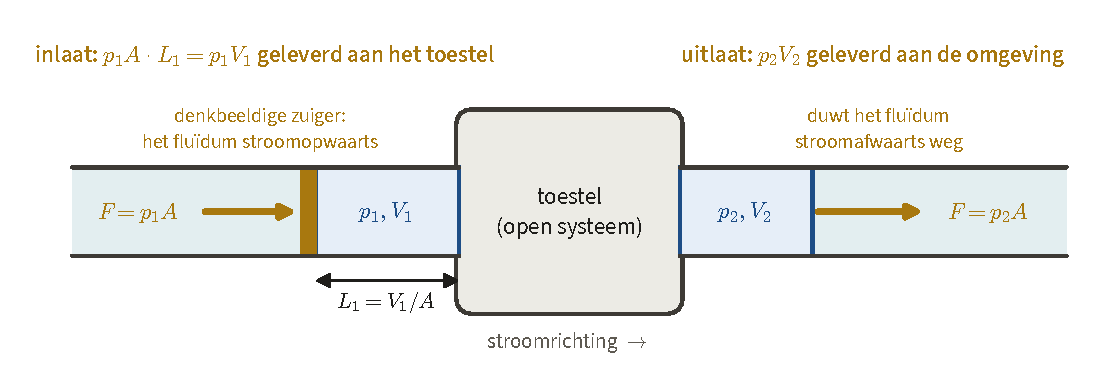
\includegraphics[width=\textwidth]{Figuren/stromingsarbeid}
    \caption{Stromingsarbeid. Aan de inlaat duwt het flu\"idum stroomopwaarts als een denkbeeldige zuiger een pakketje met kracht $p_1A$ over zijn lengte $L_1 = V_1/A$ naar binnen: het toestel ontvangt arbeid $p_1V_1$. Aan de uitlaat duwt het uittredende pakketje het flu\"idum stroomafwaarts weg: het toestel levert arbeid $p_2V_2$.}
    \label{fig:stromingsarbeid}
\end{figure}

\begin{definitie}{Enthalpie}
\begin{equation}
H = U + pV
\end{equation}
\end{definitie}

Differenti\"eren en de eerste hoofdwet invullen geeft $\dd H = \delta Q + V\,\dd p$. Bij \emph{constante druk} valt de laatste term weg:
\begin{equation}
\dd H = \delta Q_p .
\end{equation}
De enthalpieverandering is dus de warmte bij constante druk. Omdat de meeste processen bij (nagenoeg) constante druk lopen, rekenen ingenieurs bijna altijd met $H$: warmtewisselaars, kolommen en reactoren worden ontworpen met enthalpiebalansen. Voor vaste stoffen en vloeistoffen is $pV$ klein, zodat $\Delta H \approx \Delta U$; voor gassen is het verschil $\Delta(pV) = \Delta n_\text{gas}RT$.

Waar gaat dat verschil naartoe? Stel dat een reactie bij constante druk $p$ in een cilinder met een vrij bewegende zuiger loopt (figuren~\ref{fig:enthalpie-thermolyse} en~\ref{fig:enthalpie-vet}). Ontstaat er gas, dan schuift de zuiger op en duwt het systeem de atmosfeer weg: het levert arbeid $W = -p\,\Delta V$. Verdwijnt er gas, dan duwt de atmosfeer de zuiger in en krijgt het systeem arbeid. Met de ideale gaswet is $p\,\Delta V = \Delta n_\text{gas}RT$ (het volume van vaste stoffen en vloeistoffen verwaarlozen we), zodat de eerste hoofdwet $\Delta U = Q_p + W$ wordt
\begin{equation}
\Delta U = \Delta H - \Delta n_\text{gas}RT .
\label{eq:dU-dH}
\end{equation}
De warmte $Q_p = \Delta H$ en de verandering van de interne energie verschillen dus precies met de volumearbeid tegen de atmosfeer. Twee reacties uit het dagelijks leven tonen beide richtingen.

\begin{voorbeeld}{Thermolyse van kalksteen: warmte erin, arbeid eruit}
In een kalkoven wordt kalksteen ontbonden tot ongebluste kalk, de grondstof voor cement en mortel:
\[
\mathrm{CaCO_3(s)} \;\longrightarrow\; \mathrm{CaO(s)} + \mathrm{CO_2(g)}, \qquad \Delta H^\circ = +\SI{178.3}{\kilo\joule\per\mole} \quad (\SI{298}{\kelvin}).
\]
\begin{figure}[H]
    \centering
    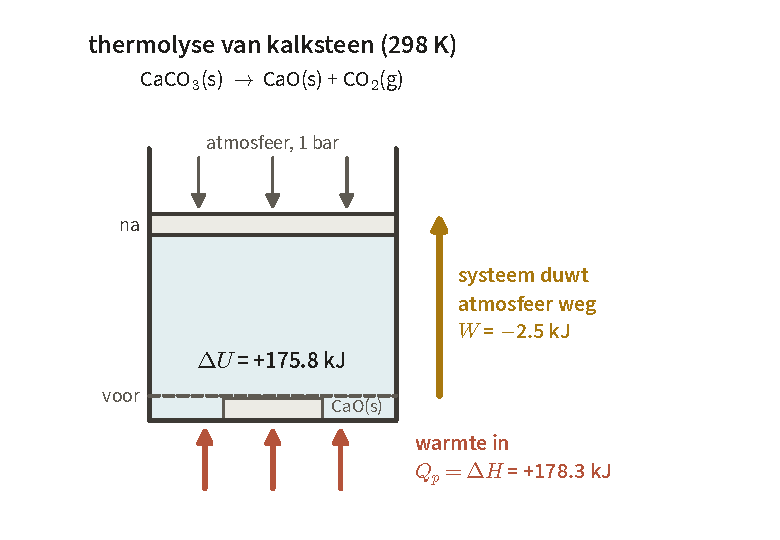
\includegraphics[width=0.75\textwidth]{Figuren/enthalpie_thermolyse}
    \caption{Thermolyse van kalksteen bij constante druk, per mol. Er ontstaat CO$_2$; de zuiger schuift op en een deel van de toegevoerde warmte verlaat het systeem weer als arbeid. Pijlen niet op schaal.}
    \label{fig:enthalpie-thermolyse}
\end{figure}
De reactie is endotherm: je moet \SI{178.3}{\kilo\joule} warmte toevoeren per mol. Er ontstaat \'e\'en mol gas uit niets dan vaste stof, dus $\Delta n_\text{gas} = +1$ en
\begin{align*}
W &= -\Delta n_\text{gas}RT = -(1)(8.314)(298) = \SI{-2.48}{\kilo\joule\per\mole},\\
\Delta U &= Q_p + W = 178.3 - 2.5 = \SI{175.8}{\kilo\joule\per\mole}.
\end{align*}
Van de toegevoerde warmte blijft dus \SI{175.8}{\kilo\joule} in het systeem (om de bindingen te herschikken) en lekt \SI{2.5}{\kilo\joule} weer weg als arbeid om de atmosfeer opzij te duwen voor het gevormde CO$_2$. In de oven, bij ongeveer \SI{900}{\celsius}, is die arbeid $RT \approx \SI{9.8}{\kilo\joule\per\mole}$: viermaal groter, maar nog steeds slechts enkele procent van de reactie-enthalpie.
\end{voorbeeld}

\begin{voorbeeld}{Verbranding van vet: warmte eruit, arbeid erin}
Je lichaam verbrandt vet, bijvoorbeeld tristearine, bij lichaamstemperatuur (\SI{310}{\kelvin}) en constante druk tot CO$_2$ en vloeibaar water:
\[
\mathrm{C_{57}H_{110}O_6(s)} + 81.5\,\mathrm{O_2(g)} \;\longrightarrow\; 57\,\mathrm{CO_2(g)} + 55\,\mathrm{H_2O(l)}, \qquad \Delta H \approx \SI{-35700}{\kilo\joule\per\mole}.
\]
\begin{figure}[H]
    \centering
    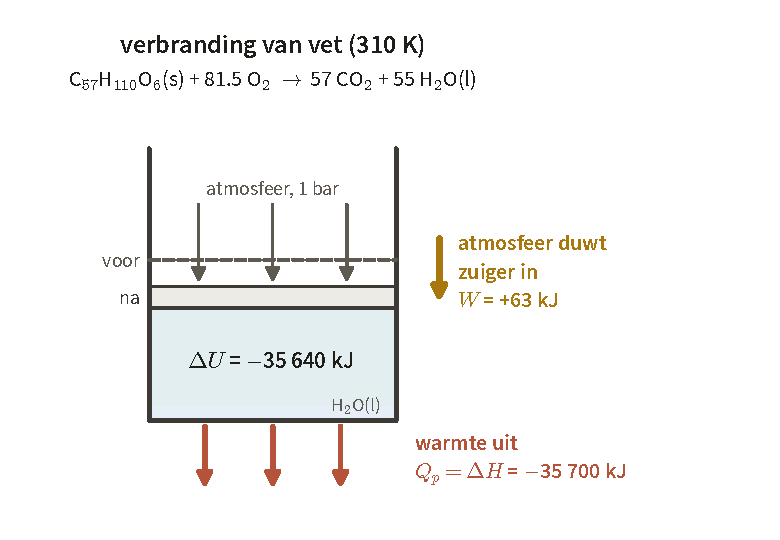
\includegraphics[width=0.75\textwidth]{Figuren/enthalpie_vet}
    \caption{Verbranding van tristearine bij constante druk, per mol. Er verdwijnt gas; de atmosfeer duwt de zuiger in en levert arbeid, zodat er meer warmte vrijkomt dan de interne energie daalt. Pijlen niet op schaal.}
    \label{fig:enthalpie-vet}
\end{figure}
Dat is ongeveer \SI{40}{\kilo\joule} per gram vet ($M = \SI{891.5}{\gram\per\mole}$). Hier \emph{verdwijnt} gas: $\Delta n_\text{gas} = 57 - 81.5 = -24.5$. De atmosfeer duwt het volume dus samen en levert arbeid aan het systeem:
\begin{align*}
W &= -\Delta n_\text{gas}RT = -(-24.5)(8.314)(310) = \SI{+63}{\kilo\joule\per\mole},\\
\Delta U &= Q_p + W = -35\,700 + 63 = \SI{-35640}{\kilo\joule\per\mole}.
\end{align*}
De vrijgekomen warmte ($|Q_p| = \SI{35700}{\kilo\joule}$) is dus \emph{groter} dan de daling van de interne energie ($\SI{35640}{\kilo\joule}$): de \SI{63}{\kilo\joule} arbeid die de omgeving levert, komt er als warmte bij. Er lekt hier niets weg; het is precies omgekeerd als bij de kalkoven. Het effect is klein (\SI{0.2}{\percent}), wat bevestigt dat $\Delta H \approx \Delta U$ voor de meeste reacties, maar het teken van $\Delta n_\text{gas}$ bepaalt in welke richting de arbeid loopt.
\end{voorbeeld}

\section{Warmtecapaciteiten}
\label{sec:warmtecapaciteiten}

Om een stof op te warmen is warmte nodig. De \emph{warmtecapaciteit} geeft aan hoeveel energie moet worden toegevoerd om de temperatuur van een systeem met \'e\'en kelvin te verhogen:
\begin{equation}
C = \frac{\dd Q}{\dd T}
\end{equation}

De \emph{warmtecapaciteit} is de warmte die nodig is om de temperatuur met \'e\'en kelvin te verhogen. Omdat warmte een padfunctie is, zijn er twee versies:
\begin{equation}
C_V = \left(\frac{\partial U}{\partial T}\right)_V
\qquad\qquad
C_p = \left(\frac{\partial H}{\partial T}\right)_p
\end{equation}
Bij constante druk zet het systeem bij opwarming uit en levert het arbeid, dus is meer warmte nodig: $C_p > C_V$. Hoeveel meer, volgt voor een ideaal gas rechtstreeks uit de definitie van enthalpie.

\begin{enumerate}
\item Vertrek van $H = U + pV$ en vul de ideale gaswet $pV = nRT$ in:
\[
H = U + nRT .
\]
\item Bij een ideaal gas oefenen de moleculen geen krachten op elkaar uit. De interne energie hangt dan enkel van de temperatuur af, niet van het volume of de druk: $U = U(T)$. Daardoor is ook $H = U(T) + nRT$ enkel een functie van $T$, en mag je de parti\"ele afgeleiden in de definities van $C_V$ en $C_p$ vervangen door gewone afgeleiden:
\[
C_V = \frac{\dd U}{\dd T}, \qquad C_p = \frac{\dd H}{\dd T}.
\]
\item Leid $H = U + nRT$ af naar $T$ ($n$ en $R$ zijn constant):
\[
\frac{\dd H}{\dd T} = \frac{\dd U}{\dd T} + nR
\qquad\Longrightarrow\qquad
C_p = C_V + nR .
\]
\item Deel door $n$ voor de molaire grootheden. Dat is de \emph{wet van Mayer}:
\begin{equation}
C_{p,\mathrm{m}} - C_{V,\mathrm{m}} = R .
\label{eq:mayer}
\end{equation}
\end{enumerate}
De term $nR$ heeft een eenvoudige betekenis: het is de arbeid die het gas per kelvin levert wanneer het bij constante druk uitzet, want $p\,\Delta V = nR\,\Delta T$. Voor \SI{1}{\mole} gas is dat \SI{8.314}{\joule} per kelvin, die je bij constante druk extra moet toevoeren bovenop wat naar de interne energie gaat. Voor vaste stoffen en vloeistoffen is de uitzetting zo klein dat $C_p \approx C_V$.
Een \'e\'enatomig gas heeft $C_{V,\mathrm{m}} = \tfrac{3}{2}R$ (enkel translatie); twee- en meeratomige gassen hebben meer, omdat ook rotatie en vibratie energie opnemen (\S~\ref{sec:moleculaire-beweging}).

\begin{voorbeeld}{Opwarmen van water versus lucht}
Om \SI{1}{\kilogram} op te warmen van \SI{20}{\celsius} naar \SI{30}{\celsius} heeft water ($c_p = \SI{4.18}{\kilo\joule\per\kilogram\per\kelvin}$) \SI{41.8}{\kilo\joule} nodig, lucht ($c_p = \SI{1.00}{\kilo\joule\per\kilogram\per\kelvin}$) slechts \SI{10.0}{\kilo\joule}. Per kilogram neemt water dus vier keer meer warmte op: daarom is het zo'n goede koelvloeistof.
\end{voorbeeld}

\subsection{Toepassing: waarom wordt een compressor warm?}
\label{sec:compressor}

Persluchtinstallaties, koelmachines en warmtepompen, de aardgastransportleiding: overal wordt gas gecomprimeerd. De gecomprimeerde lucht van een werkplaatscompressor verlaat de compressor gloeiend heet. Met de eerste hoofdwet en de warmtecapaciteit kunnen we nu berekenen hoe heet, en waarom dat ingenieurs zorgen baart.

\paragraph{Stap 1: de compressie is adiabatisch.}
Een gaspakketje doorloopt een compressor in een fractie van een seconde. Warmteoverdracht naar de wand is daarvoor veel te traag, zodat $Q \approx 0$. De eerste hoofdwet voor dat pakketje wordt dan $\dd U = \delta W = -p\,\dd V$: alle arbeid blijft als interne energie in het gas.

\paragraph{Stap 2: van arbeid naar temperatuur.}
Voor een ideaal gas is $\dd U = nC_{V,\mathrm{m}}\,\dd T$ en $p = nRT/V$. Invullen en scheiden van de veranderlijken geeft
\[
C_{V,\mathrm{m}}\,\frac{\dd T}{T} = -R\,\frac{\dd V}{V}
\qquad\Longrightarrow\qquad
\ln\frac{T_2}{T_1} = -\frac{R}{C_{V,\mathrm{m}}}\ln\frac{V_2}{V_1}.
\]
Het volume is in een compressor moeilijk te meten, de druk wel. Vervang daarom $V_2/V_1 = (T_2/T_1)(p_1/p_2)$ en gebruik $C_{V,\mathrm{m}} + R = C_{p,\mathrm{m}}$:
\begin{equation}
\boxed{\;\frac{T_2}{T_1} = \left(\frac{p_2}{p_1}\right)^{R/C_{p,\mathrm{m}}}\;}
\label{eq:adiabatische-compressie}
\end{equation}
De temperatuurstijging hangt dus enkel af van de \emph{drukverhouding}, niet van de absolute druk. Lucht bestaat uit tweeatomige moleculen met $C_{p,\mathrm{m}} \approx \tfrac{7}{2}R$, zodat $R/C_{p,\mathrm{m}} = 2/7 = 0.286$.

\paragraph{Stap 3: hoe warm?}
Lucht van \SI{20}{\celsius} wordt van \SI{1}{\bar} naar \SI{8}{\bar} gebracht, een gewone werkplaatsdruk:
\[
T_2 = (293.15)\,(8)^{0.286} = \SI{531}{\kelvin} = \SI{258}{\celsius}.
\]
Een re\"ele compressor heeft bovendien wrijving en verliezen, waardoor de lucht nog warmer wordt. Bij die temperatuur ontleedt smeerolie en vormt ze afzettingen, en in het ergste geval ontvlamt de oliedamp. De eindtemperatuur is daarom een harde ontwerpgrens.

\paragraph{Stap 4: hoeveel arbeid?}
Een compressor is een open systeem. Volgens \S~\ref{sec:enthalpie} is $\dd H = \delta Q + V\,\dd p$; zonder warmte-uitwisseling is de arbeid die de compressor per mol levert dus gelijk aan de enthalpiestijging van het gas:
\[
W_\text{adiabatisch} = \Delta H_\mathrm{m} = C_{p,\mathrm{m}}(T_2 - T_1) = \tfrac{7}{2}(8.314)(531 - 293) = \SI{6.92}{\kilo\joule\per\mole}.
\]
Zou je het gas tijdens de compressie perfect koelen (isotherm), dan is $W = \int V\,\dd p = RT\ln(p_2/p_1) = (8.314)(293)\ln 8 = \SI{5.07}{\kilo\joule\per\mole}$. De adiabatische compressie kost dus \SI{37}{\percent} meer arbeid. De reden zie je in $\int V\,\dd p$: het opgewarmde gas neemt bij elke druk een groter volume in, en dat volume moet de compressor verder samendrukken. In figuur~\ref{fig:compressie} is dat het gekleurde vlak tussen beide curven.

\paragraph{Stap 5: de oplossing is tussenkoeling.}
Perfect koelen tijdens de compressie lukt niet, maar je kan de compressie wel in stukken hakken. Een tweetrapscompressor brengt de lucht eerst van \SI{1}{\bar} naar \SI{2.83}{\bar} (drukverhouding $\sqrt{8}$), koelt ze in een \emph{tussenkoeler} terug tot \SI{20}{\celsius}, en comprimeert dan verder naar \SI{8}{\bar}. Elke trap haalt nu
\[
T = (293.15)\,(2.83)^{0.286} = \SI{395}{\kelvin} = \SI{121}{\celsius},
\]
en de totale arbeid daalt tot $2 \cdot \tfrac{7}{2}(8.314)(395 - 293) = \SI{5.90}{\kilo\joule\per\mole}$: \SI{15}{\percent} minder dan zonder tussenkoeling. De groene weg in figuur~\ref{fig:compressie} benadert de isotherm des te beter naarmate er meer trappen zijn. Daarom hebben compressoren voor hoge drukken, zoals die voor het vullen van duikflessen (\SI{200}{\bar}) of voor de ammoniaksynthese (150 tot \SI{300}{\bar}), drie tot vijf trappen met telkens een tussenkoeler.

\begin{figure}[htb]
    \centering
    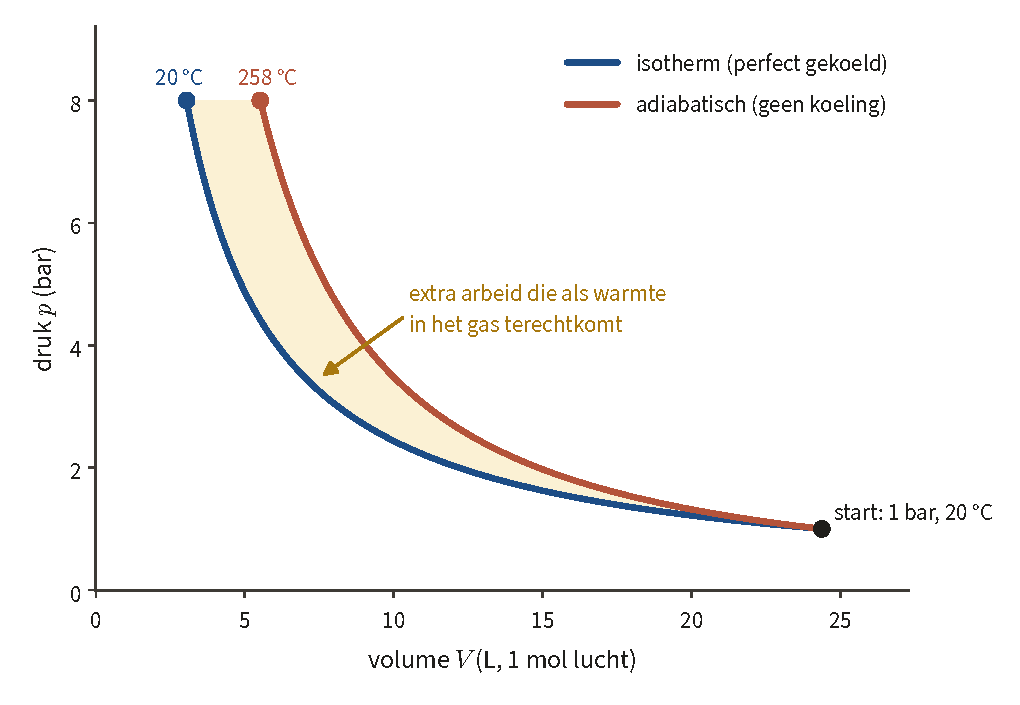
\includegraphics[width=0.75\linewidth]{Figuren/compressie_pv}
    \caption{Compressie van \SI{1}{\mole} lucht van \SI{1}{\bar} naar \SI{8}{\bar}, vertrekkend van \SI{20}{\celsius}. Isotherm: het gas wordt perfect gekoeld. Adiabatisch: alle arbeid blijft als interne energie in het gas. Tweetraps: adiabatisch tot \SI{2.83}{\bar}, terugkoelen tot \SI{20}{\celsius}, opnieuw adiabatisch. Het gekleurde vlak is de extra arbeid van de adiabatische compressie ten opzichte van de isotherme.}
    \label{fig:compressie}
\end{figure}

Hetzelfde effect benut men in een dieselmotor. Daar wordt lucht snel samengedrukt tot een twintigste van haar volume. Met vergelijking~\eqref{eq:adiabatische-compressie} herschreven naar volumes, $T_2/T_1 = (V_1/V_2)^{R/C_{V,\mathrm{m}}}$, loopt ze op van \SI{20}{\celsius} tot bijna \SI{700}{\celsius}, heet genoeg om de ingespoten diesel zonder bougie te ontsteken. Het omgekeerde voel je wanneer je lucht uit een fietsband laat ontsnappen: bij een snelle (adiabatische) expansie levert het gas arbeid, en daalt zijn temperatuur.



\section{Temperatuurafhankelijkheid van de enthalpie}

Bij opwarmen bij constante druk neemt de enthalpie toe volgens
\begin{equation}
\Delta H = \int_{T_1}^{T_2} C_p(T)\,\dd T \;\approx\; C_p\,(T_2-T_1) \quad\text{(als $C_p$ ongeveer constant is).}
\end{equation}
Over een groot temperatuurbereik is $C_p$ niet constant: hoe warmer, hoe meer vibraties worden aangeslagen, zodat $C_p$ stijgt (figuur~\ref{fig:cp-temperatuur}). Eenatomige gassen zoals helium hebben geen vibraties en dus een constante $C_p = \tfrac{5}{2}R$. Voor nauwkeurige berekeningen gebruikt men een empirische veelterm,
\begin{equation}
C_{p,\mathrm{m}} = a+bT+cT^2 ,
\end{equation}
met co\"effici\"enten zoals in tabel~\ref{tab:cp_coeff}. Processimulatoren (Aspen Plus, CHEMCAD) bevatten uitgebreide databanken van zulke correlaties.

\begin{figure}[htb]
    \centering
    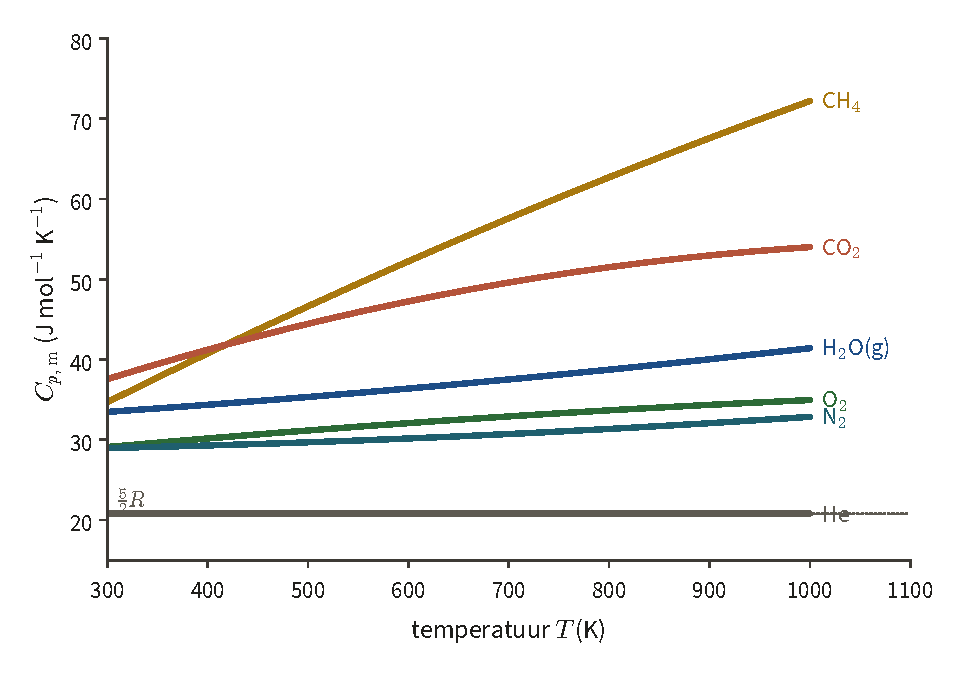
\includegraphics[width=0.7\linewidth]{Figuren/cp_temperatuur}
    \caption{Molaire warmtecapaciteit van enkele gassen tussen \SI{300}{\kelvin} en \SI{1000}{\kelvin} (correlaties uit tabel~\ref{tab:cp_coeff}, bron NIST). Hoe meer atomen, hoe meer vibraties en hoe sterker $C_p$ stijgt; helium blijft vlak op $\tfrac{5}{2}R$.}
    \label{fig:cp-temperatuur}
\end{figure}

\begin{table}[htb]
\centering
\caption{Benaderende co\"effici\"enten voor $C_{p,\mathrm{m}} = a + bT + cT^2$ (in \si{\joule\per\mole\per\kelvin}, $T$ in \si{\kelvin}), geldig tussen \SI{300}{\kelvin} en \SI{1000}{\kelvin} (afwijking kleiner dan \SI{1}{\joule\per\mole\per\kelvin}).
\label{tab:cp_coeff}
\begin{tabular}{lccc}
\toprule
Component & $a$ & $b$ & $c$ \\
\midrule
\ce{N2}     & 28.5 & $3.6\times10^{-4}$  & $4.00\times10^{-6}$ \\
\ce{O2}     & 25.4 & $1.35\times10^{-2}$ & $-3.95\times10^{-6}$ \\
Lucht       & 27.8 & $3.12\times10^{-3}$ & $2.33\times10^{-6}$ \\
\ce{H2}     & 29.1 & $-6.1\times10^{-4}$ & $1.65\times10^{-6}$ \\
\ce{CO}     & 27.7 & $3.12\times10^{-3}$ & $2.47\times10^{-6}$ \\
\ce{CO2}    & 23.9 & $5.21\times10^{-2}$ & $-2.20\times10^{-5}$ \\
\ce{CH4}    & 14.9 & $6.96\times10^{-2}$ & $-1.23\times10^{-5}$ \\
\ce{H2O(g)} & 31.3 & $5.99\times10^{-3}$ & $4.12\times10^{-6}$ \\
\ce{NH3}    & 24.4 & $3.86\times10^{-2}$ & $-6.40\times10^{-6}$ \\
He          & 20.8 & 0                   & 0 \\
\bottomrule
\end{tabular}
\end{table}

\begin{voorbeeld}{Enthalpieverandering van lucht}
Lucht wordt bij constante druk opgewarmd van \SI{300}{\kelvin} naar \SI{600}{\kelvin}. Term per term integreren:
\begin{align*}
\Delta H_\mathrm{m} &= a(T_2-T_1) + \frac{b}{2}(T_2^2-T_1^2) + \frac{c}{3}(T_2^3-T_1^3)\\
&= 27.8(300) + \frac{3.12\times10^{-3}}{2}(600^2-300^2) + \frac{2.33\times10^{-6}}{3}(600^3-300^3)\\
&= 8350 + 421 + 147 = \SI{8.92}{\kilo\joule\per\mole}.
\end{align*}
Met een constante $C_{p,\mathrm{m}} = \SI{29.7}{\joule\per\mole\per\kelvin}$ (de waarde bij \SI{450}{\kelvin}, halfweg) vind je \SI{8.90}{\kilo\joule\per\mole}; met de waarde bij \SI{300}{\kelvin} (\SI{29.0}{\joule\per\mole\per\kelvin}) \SI{8.70}{\kilo\joule\per\mole}, nog geen \SI{3}{\percent} te weinig. Een gemiddelde $C_p$ volstaat dus vaak; de veelterm wordt belangrijk bij grote temperatuursprongen, zoals in een vlam (\S~\ref{sec:warmte-effecten}).
\end{voorbeeld}

\section{Standaardtoestanden en de wet van Hess}
\label{sec:hess}

Enthalpie\"en worden altijd opgegeven ten opzichte van een \emph{standaardtoestand}: zuivere stof bij \SI{1}{\bar}, meestal getabelleerd bij \SI{298.15}{\kelvin}. De \emph{standaardvormingsenthalpie} $\Delta H_f^\circ$ is de enthalpieverandering wanneer \'e\'en mol van een stof gevormd wordt uit de elementen in hun standaardtoestand. Voor die elementen zelf is $\Delta H_f^\circ = 0$. Omdat $H$ een toestandsfunctie is, mag je elke reactie opsplitsen in ``ontbinden tot elementen'' en ``opbouwen tot producten'' (figuur~\ref{fig:hess}). Dat is de \emph{wet van Hess}:
\begin{equation}
\Delta_r H^\circ = \sum_i \nu_i\, \Delta H_{f,i}^\circ ,
\end{equation}
met $\nu_i$ positief voor producten en negatief voor reagentia. Op dezelfde manier worden standaardentropie\"en $S^\circ$ en vormings-Gibbsenergie\"en $\Delta G_f^\circ$ getabelleerd (hoofdstuk~\ref{ch:spontaniteit}).

\begin{figure}[htb]
    \centering
    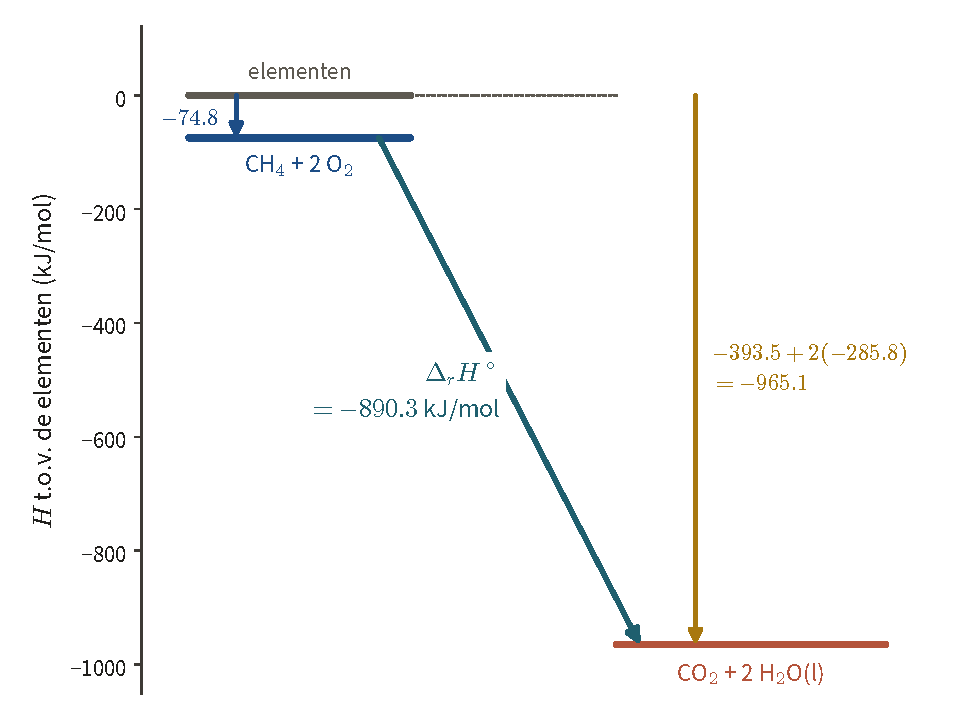
\includegraphics[width=0.7\linewidth]{Figuren/hess}
    \caption{Enthalpiediagram voor de verbranding van methaan. De elementen liggen per definitie op nul. De reactie-enthalpie is het verschil tussen het niveau van de producten en dat van de reagentia, welke weg je ook volgt.}
    \label{fig:hess}
\end{figure}

\begin{voorbeeld}{Reactie-enthalpie via de wet van Hess}
Voor \ce{CH4(g) + 2 O2(g) -> CO2(g) + 2 H2O(l)} met $\Delta H_f^\circ$ = $-74.8$ (\ce{CH4}), $-393.5$ (\ce{CO2}) en $-285.8$ (\ce{H2O(l)}) \si{\kilo\joule\per\mole}:
\[
\Delta_r H^\circ = (-393.5) + 2(-285.8) - (-74.8) = \SI{-890.3}{\kilo\joule\per\mole}.
\]
Per mol methaan komt \SI{890.3}{\kilo\joule} vrij: de basis voor het ontwerp van elke aardgasbrander.
\end{voorbeeld}

\section{Temperatuurafhankelijkheid van reactie-enthalpie\"en: de wet van Kirchhoff}
\label{sec:kirchhoff}

Tabellen geven reactie- en vormingsenthalpie\"en bij \SI{298}{\kelvin}, maar reacties lopen zelden bij kamertemperatuur. Ammoniak wordt gemaakt bij ongeveer \SI{450}{\celsius}, methanol bij \SI{250}{\celsius}, kalk bij \SI{900}{\celsius}. Hoe reken je de reactie-enthalpie om naar de procestemperatuur?

\paragraph{Afleiding met een kringloop.} Omdat $H$ een toestandsfunctie is, mag je van reagentia bij $T_0 = \SI{298}{\kelvin}$ naar producten bij een andere temperatuur $T$ gaan langs elke weg die je wil. Vergelijk twee wegen:
\begin{enumerate}
\item \emph{Eerst reageren, dan opwarmen.} Laat de reactie verlopen bij $T_0$ en warm daarna de producten op van $T_0$ tot $T$:
\[
\Delta H_\text{weg 1} = \Delta_r H^\circ(T_0) + \int_{T_0}^{T} C_{p,\text{producten}}\,\dd T .
\]
\item \emph{Eerst opwarmen, dan reageren.} Warm de reagentia op van $T_0$ tot $T$ en laat de reactie daar verlopen:
\[
\Delta H_\text{weg 2} = \int_{T_0}^{T} C_{p,\text{reagentia}}\,\dd T + \Delta_r H^\circ(T) .
\]
\item Begin- en eindtoestand zijn dezelfde, dus $\Delta H_\text{weg 1} = \Delta H_\text{weg 2}$. Oplossen naar $\Delta_r H^\circ(T)$ geeft de \emph{wet van Kirchhoff}:
\begin{equation}
\boxed{\;\Delta_r H^\circ(T) = \Delta_r H^\circ(T_0) + \int_{T_0}^{T} \Delta_r C_p^\circ\,\dd T\;}
\label{eq:kirchhoff}
\end{equation}
met
\[
\Delta_r C_p^\circ = \sum_\text{producten} \nu\, C_{p,\mathrm{m}}^\circ - \sum_\text{reagentia} \nu\, C_{p,\mathrm{m}}^\circ .
\]
\end{enumerate}
In differentiaalvorm staat er $\dd(\Delta_r H^\circ)/\dd T = \Delta_r C_p^\circ$: de reactie-enthalpie verandert met de temperatuur precies zo snel als het verschil in warmtecapaciteit tussen producten en reagentia.

\paragraph{Grafisch.} Teken de enthalpie van de reagentia en van de producten als functie van $T$ (figuur~\ref{fig:kirchhoff}, links). Elke lijn stijgt met een helling gelijk aan de totale warmtecapaciteit, en de verticale afstand tussen beide lijnen is $\Delta_r H^\circ(T)$. De twee wegen uit de afleiding zijn de twee manieren om van het blauwe punt linksboven naar het rode punt rechtsonder te gaan: eerst omlaag en dan langs de rode lijn, of eerst langs de blauwe lijn en dan omlaag. Lopen de lijnen evenwijdig ($\Delta_r C_p = 0$), dan hangt $\Delta_r H$ niet van de temperatuur af. Hebben de reagentia de grotere warmtecapaciteit, zoals bij de ammoniaksynthese, dan gaan de lijnen uit elkaar en wordt de reactie bij hogere temperatuur sterker exotherm.

\begin{figure}[htb]
    \centering
    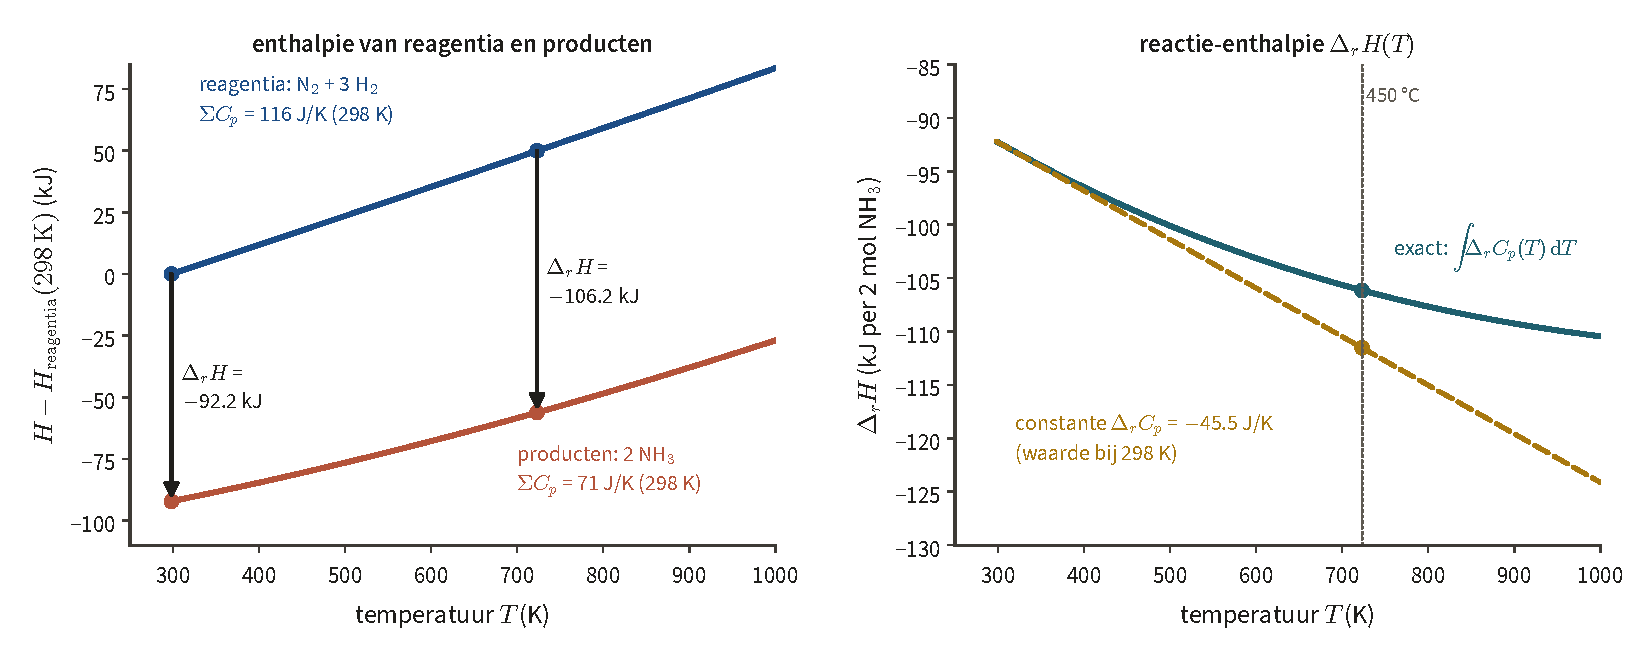
\includegraphics[width=\textwidth]{Figuren/kirchhoff}
    \caption{De wet van Kirchhoff voor de ammoniaksynthese \ce{N2 + 3 H2 -> 2 NH3}. Links: enthalpie van reagentia en producten (ten opzichte van de reagentia bij \SI{298}{\kelvin}); de helling van elke lijn is zijn warmtecapaciteit, de verticale afstand is $\Delta_r H$. Rechts: $\Delta_r H(T)$ met de temperatuurafhankelijke $C_p$ uit tabel~\ref{tab:cp_coeff} en met de constante waarde $\Delta_r C_p(\SI{298}{\kelvin})$.}
    \label{fig:kirchhoff}
\end{figure}

\paragraph{Constante $\Delta_r C_p$.} Over een beperkt temperatuurinterval mag je $\Delta_r C_p^\circ$ constant nemen, en dan wordt de integraal eenvoudig:
\begin{equation}
\Delta_r H^\circ(T) \approx \Delta_r H^\circ(T_0) + \Delta_r C_p^\circ\,(T - T_0).
\label{eq:kirchhoff-constant}
\end{equation}
Dat is een rechte in figuur~\ref{fig:kirchhoff} (rechts). Hoe groter het temperatuurverschil, hoe meer ze afwijkt van de echte kromme, omdat de warmtecapaciteiten zelf met $T$ veranderen (figuur~\ref{fig:cp-temperatuur}).

\begin{voorbeeld}{Vormingsenthalpie van waterdamp bij \SI{100}{\celsius}}
De standaardvormingsenthalpie van waterdamp bij \SI{25}{\celsius} is \SI{-241.82}{\kilo\joule\per\mole}. Hoeveel is ze bij \SI{100}{\celsius}? De vormingsreactie is
\[
\ce{H2(g) + 1/2 O2(g) -> H2O(g)}.
\]
Met $C_{p,\mathrm{m}}^\circ$ bij \SI{298}{\kelvin} (\ce{H2O(g)} 33.58, \ce{H2} 28.82, \ce{O2} \SI{29.36}{\joule\per\mole\per\kelvin}; Atkins \& de Paula):
\[
\Delta_r C_p^\circ = 33.58 - 28.82 - \tfrac12(29.36) = \SI{-9.92}{\joule\per\mole\per\kelvin}.
\]
Over \SI{75}{\kelvin} is $\Delta_r C_p$ zeker constant, dus
\[
\Delta_f H^\circ(\SI{373}{\kelvin}) = -241.82 + (-9.92\times10^{-3})(75) = \SI{-242.56}{\kilo\joule\per\mole}.
\]
Een verschuiving van amper \SI{0.3}{\percent}: over enkele tientallen kelvin mag je de tabelwaarde meestal gewoon gebruiken.
\end{voorbeeld}

\begin{voorbeeld}{Ammoniaksynthese bij \SI{450}{\celsius}}
In het Haber-Boschproces reageert \ce{N2 + 3 H2 -> 2 NH3} bij ongeveer \SI{723}{\kelvin}. Bij \SI{298}{\kelvin} is $\Delta_r H^\circ = 2(\SI{-46.1}{\kilo\joule\per\mole}) = \SI{-92.2}{\kilo\joule}$. Hoeveel warmte moet de koeling van de reactor per 2 mol \ce{NH3} afvoeren bij de procestemperatuur?

\emph{Stap 1: $\Delta_r C_p$ als veelterm.} Met $C_p = a + bT + cT^2$ uit tabel~\ref{tab:cp_coeff} combineer je de co\"effici\"enten zoals de stoffen in de reactie:
\begin{align*}
\Delta a &= 2(24.4) - 28.5 - 3(29.1) = -67.0,\\
\Delta b &= 2(3.86\times10^{-2}) - 3.6\times10^{-4} - 3(-6.1\times10^{-4}) = 7.87\times10^{-2},\\
\Delta c &= 2(-6.40\times10^{-6}) - 4.00\times10^{-6} - 3(1.65\times10^{-6}) = -2.18\times10^{-5}.
\end{align*}
Bij \SI{298}{\kelvin} is $\Delta_r C_p = \SI{-45.5}{\joule\per\kelvin}$, bij \SI{723}{\kelvin} nog maar \SI{-21.5}{\joule\per\kelvin}.

\emph{Stap 2: integreren} van \SI{298}{\kelvin} tot \SI{723}{\kelvin}, term per term zoals bij de opwarming van lucht:
\begin{align*}
\int_{298}^{723} \Delta_r C_p\,\dd T &= \Delta a\,(425) + \frac{\Delta b}{2}(723^2 - 298^2) + \frac{\Delta c}{3}(723^3 - 298^3)\\
&= -28.5 + 17.1 - 2.5 = \SI{-14.0}{\kilo\joule}.
\end{align*}
\emph{Stap 3: optellen.}
\[
\Delta_r H^\circ(\SI{723}{\kelvin}) = -92.2 - 14.0 = \SI{-106.2}{\kilo\joule}.
\]
Bij de procestemperatuur komt dus \SI{15}{\percent} meer warmte vrij dan de tabelwaarde doet vermoeden, en dat moet de koeling aankunnen. Had je $\Delta_r C_p$ constant op zijn waarde bij \SI{298}{\kelvin} gehouden, dan vond je $-92.2 + (-45.5\times10^{-3})(425) = \SI{-111.5}{\kilo\joule}$: de fout van \SI{5}{\kilo\joule} is ruim een derde van de correctie zelf (figuur~\ref{fig:kirchhoff}, rechts). Over honderden kelvin gebruik je dus beter de temperatuurafhankelijke $C_p$.
\end{voorbeeld}


\section{Warmte-effecten van reacties: de adiabatische temperatuur}
\label{sec:warmte-effecten}

Een reactie-enthalpie uit een tabel lijkt een abstract getal. In een reactor wordt ze heel concreet: de vrijgekomen warmte moet ergens heen. Ofwel wordt ze afgevoerd via een koelmantel of warmtewisselaar, ofwel blijft ze in het reactiemengsel en stijgt de temperatuur. Voor de ingenieur is de belangrijkste vraag dan: \emph{hoe warm wordt het mengsel als er niet gekoeld wordt?}

\subsection{De energiebalans over een reactor}

Omdat enthalpie een toestandsfunctie is, mogen we de weg van reagentia naar producten zelf kiezen. De eenvoudigste weg bestaat uit twee stappen:
\begin{enumerate}
\item de reactie laten verlopen bij \SI{298}{\kelvin}: de enthalpie verandert met $\xi\,\Delta_r H^\circ(\SI{298}{\kelvin})$, met $\xi$ het aantal mol omgezet;
\item het productmengsel opwarmen van \SI{298}{\kelvin} tot de eindtemperatuur $T$: de enthalpie verandert met $\sum_i n_i \int_{298}^{T} C_{p,i}\,\dd T$, gesommeerd over alle stoffen die de reactor verlaten (ook inerte stoffen zoals stikstof).
\end{enumerate}
Bij een \emph{adiabatische} reactor ($Q = 0$, geen asarbeid) is de totale enthalpieverandering nul. De eindtemperatuur, de \emph{adiabatische temperatuur} $T_\mathrm{ad}$, volgt dus uit
\begin{equation}
\boxed{\;0 = \xi\,\Delta_r H^\circ(\SI{298}{\kelvin}) + \sum_{i,\,\mathrm{uit}} n_i \int_{298}^{T_\mathrm{ad}} C_{p,i}\,\dd T\;}
\label{eq:adiabatische-temperatuur}
\end{equation}
Bij een exotherme reactie is de eerste term negatief; de tweede term moet die compenseren door een temperatuurstijging. Met een gemiddelde, constante warmtecapaciteit van het productmengsel wordt dit eenvoudig:
\begin{equation}
T_\mathrm{ad} - 298 \approx \frac{\xi\,(-\Delta_r H^\circ)}{\sum_i n_i \overline{C}_{p,i}}.
\label{eq:adiabatische-temperatuur-cp}
\end{equation}
Komt de voeding niet binnen op \SI{298}{\kelvin}, dan voeg je een derde stap toe: de voeding eerst afkoelen (of opwarmen) tot \SI{298}{\kelvin}.

\begin{voorbeeld}{Adiabatische vlamtemperatuur van aardgas}
Methaan verbrandt met de stoichiometrische hoeveelheid lucht (\SI{21}{\percent} \ce{O2}, \SI{79}{\percent} \ce{N2}, dus 3.76 mol \ce{N2} per mol \ce{O2}). Voeding en lucht komen binnen op \SI{25}{\celsius}:
\[
\ce{CH4 + 2 O2 + 7.52 N2 -> CO2 + 2 H2O(g) + 7.52 N2}
\]
Het water verlaat de vlam als damp, dus gebruiken we $\Delta_r H^\circ = \SI{-802.3}{\kilo\joule\per\mole}$ (en niet $-890.3$, dat geldt voor vloeibaar water; het verschil is $2\times\SI{44.0}{\kilo\joule\per\mole}$ verdampingsenthalpie).

Als gemiddelde warmtecapaciteiten tussen \SI{298}{\kelvin} en \SI{2300}{\kelvin} nemen we \ce{CO2}: \SI{54.8}{}, \ce{H2O}: \SI{44.2}{} en \ce{N2}: \SI{33.5}{\joule\per\mole\per\kelvin}. Per mol methaan:
\[
\sum_i n_i\overline{C}_{p,i} = 54.8 + 2(44.2) + 7.52(33.5) = \SI{395}{\joule\per\kelvin}
\]
\[
T_\mathrm{ad} = 298 + \frac{802\,300}{395} = \SI{2330}{\kelvin}\;(\approx\SI{2060}{\celsius}).
\]
Gemeten vlamtemperaturen liggen iets lager, rond \SI{2220}{\kelvin}. Bij zulke hoge temperaturen valt een klein deel van \ce{CO2} en \ce{H2O} terug uiteen in \ce{CO}, \ce{H2} en \ce{O2} (een evenwicht, hoofdstuk~\ref{ch:reagerend}); die ontbinding slorpt warmte op.

Merk op dat bijna twee derde van de warmtecapaciteit van het rookgas afkomstig is van stikstof, dat niet eens deelneemt aan de reactie. Verbranden met zuivere zuurstof geeft daarom veel hogere temperaturen: een snijbrander met acetyleen en zuurstof haalt meer dan \SI{3300}{\kelvin}.
\end{voorbeeld}

\begin{figure}[htb]
    \centering
    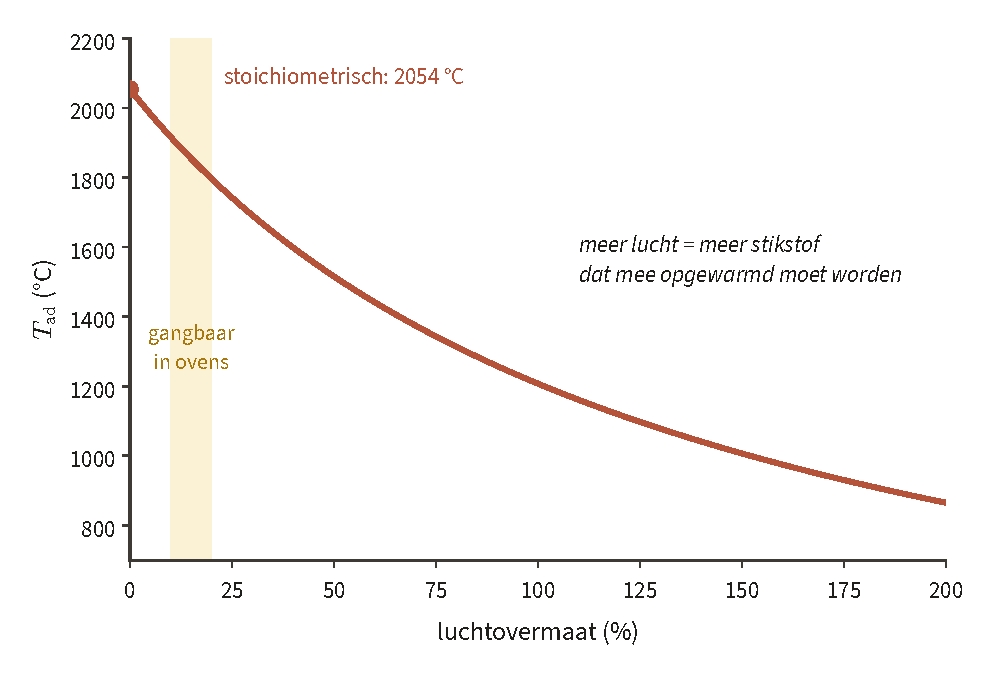
\includegraphics[width=0.7\linewidth]{Figuren/vlamtemperatuur}
    \caption{Adiabatische vlamtemperatuur van methaan als functie van de luchtovermaat, berekend met temperatuurafhankelijke warmtecapaciteiten (NIST). Elke extra kilogram lucht moet mee opgewarmd worden en verlaagt de eindtemperatuur. Ovens werken meestal met 10 tot 20\,\% luchtovermaat: genoeg om volledige verbranding te verzekeren, niet zoveel dat de vlam te sterk afkoelt.}
    \label{fig:vlamtemperatuur}
\end{figure}

\subsection{Adiabatische temperatuurstijging in een vloeistofreactor}

In een vloeistofreactor is het oplosmiddel (vaak water) de grootste warmtebuffer. Per liter reactiemengsel met beginconcentratie $c_{A,0}$ van de reagens en volumieke warmtecapaciteit $\rho c_p$ wordt vergelijking~(\ref{eq:adiabatische-temperatuur-cp}) bij volledige omzetting:
\begin{equation}
\boxed{\Delta T_\mathrm{ad} = \frac{c_{A,0}\,(-\Delta_r H)}{\rho\,c_p}}
\label{eq:delta-T-ad}
\end{equation}
Dit getal is een eerste veiligheidscontrole voor elke exotherme reactie: het is de temperatuurstijging die optreedt als de koeling volledig uitvalt.

\begin{voorbeeld}{Wat als de koeling uitvalt?}
In een batchreactor verloopt een hydrogenering in waterig midden met $c_{A,0} = \SI{2.0}{\mole\per\litre}$ en $\Delta_r H = \SI{-100}{\kilo\joule\per\mole}$. Met $\rho c_p \approx \SI{4.18}{\kilo\joule\per\litre\per\kelvin}$:
\[
\Delta T_\mathrm{ad} = \frac{(2.0)(100)}{4.18} = \SI{48}{\kelvin}.
\]
Start de reactor op \SI{60}{\celsius}, dan kan het mengsel bij uitval van de koeling tot \SI{108}{\celsius} opwarmen: boven het kookpunt van water. De druk in de reactor loopt op, en bovendien versnelt de reactie sterk bij hogere temperatuur. In hoofdstuk~\ref{ch:kinetiek} zien we hoe die combinatie kan leiden tot een \emph{thermal runaway}.

Een vuistregel uit de procesveiligheid: bij $\Delta T_\mathrm{ad}$ kleiner dan ongeveer \SI{50}{\kelvin} is het risico beperkt; bij meer dan \SI{200}{\kelvin} is een grondige veiligheidsstudie nodig.
\end{voorbeeld}

\begin{toepassing}{Tussenkoeling, opnieuw}
Bij de compressor zagen we dat tussenkoeling de eindtemperatuur beperkt. Exotherme gasreactoren werken volgens hetzelfde principe. In een zwavelzuurfabriek wordt \ce{SO2} omgezet tot \ce{SO3} in vier katalysatorbedden na elkaar. In elk bed stijgt de temperatuur adiabatisch; tussen de bedden koelt een warmtewisselaar het gas opnieuw af. De vrijgekomen warmte wordt zo meteen nuttig gebruikt om stoom te maken. Waarom de temperatuur laag moet blijven, ondanks dat de reactie dan trager verloopt, zie je in hoofdstuk~\ref{ch:reagerend}: bij een exotherme reactie daalt de evenwichtsomzetting met de temperatuur.
\end{toepassing}

\section{Faseovergangen en overgangsenthalpie\"en}

Bij smelten, verdampen of sublimeren wordt warmte opgenomen zonder dat de temperatuur verandert (figuur~\ref{fig:opwarmcurve}). De warmte per mol bij constante druk is de \emph{overgangsenthalpie}: $\Delta H_\text{fus}$ (smelten), $\Delta H_\text{vap}$ (verdampen) en $\Delta H_\text{sub} = \Delta H_\text{fus} + \Delta H_\text{vap}$ (sublimeren). Voor water is $\Delta H_\text{fus} = \SI{6.0}{\kilo\joule\per\mole}$ bij \SI{0}{\celsius} en $\Delta H_\text{vap} = \SI{40.7}{\kilo\joule\per\mole}$ bij \SI{100}{\celsius}. De energie gaat naar het verbreken van intermoleculaire bindingen (hoofdstuk~\ref{ch:intermoleculair}).

\begin{figure}[htb]
    \centering
    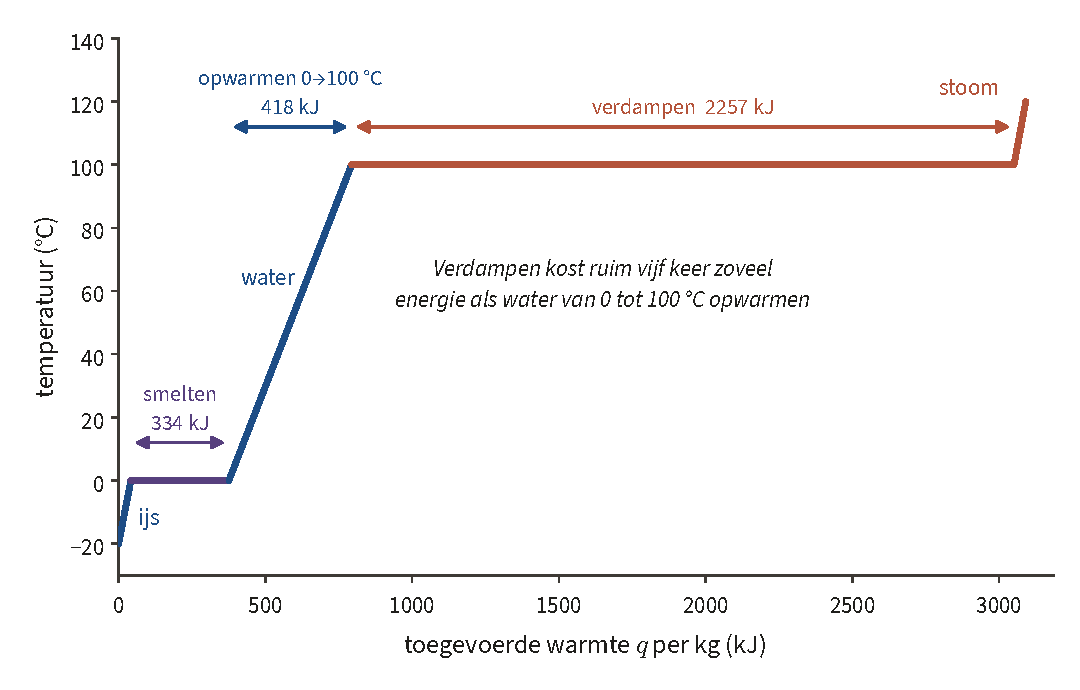
\includegraphics[width=0.7\linewidth]{Figuren/opwarmcurve_water}
    \caption{Temperatuur van \SI{1}{\kilogram} water bij gelijkmatige warmtetoevoer, van ijs bij \SI{-20}{\celsius} tot stoom bij \SI{120}{\celsius}. Tijdens smelten en verdampen blijft de temperatuur constant.}
    \label{fig:opwarmcurve}
\end{figure}

\begin{voorbeeld}{Verdampen van water}
Om \SI{1}{\mole} water op te warmen van \SI{0}{\celsius} tot \SI{100}{\celsius} is $C_p\Delta T = (75.3)(100) = \SI{7.53}{\kilo\joule}$ nodig. Om het daarna te verdampen: \SI{40.7}{\kilo\joule}, 5.4 keer meer. Van de totale \SI{48.2}{\kilo\joule} gaat dus meer dan \SI{80}{\percent} naar de faseovergang. Daarom verbruikt de reboiler van een destillatiekolom zoveel meer energie dan een gewone vloeistofverwarmer.
\end{voorbeeld}

\section{De beperkingen van de eerste hoofdwet}

Een hete kop koffie koelt af tot kamertemperatuur; nooit warmt lauwe koffie spontaan op door warmte uit de kamer te halen. Beide processen respecteren de eerste hoofdwet: energie blijft behouden. De eerste hoofdwet zegt dus niets over de \emph{richting} van een proces. Daarvoor is een tweede grootheid nodig, de entropie. Haar moleculaire oorsprong (hoofdstuk~\ref{ch:kwantum}) en haar gevolgen (hoofdstuk~\ref{ch:spontaniteit}) zijn het onderwerp van de volgende twee hoofdstukken.


\section{Samenvatting en reflectie}

\begin{samenvatting}{Energie en de eerste hoofdwet}
\begin{itemize}
\item Een \emph{systeem} is open (massa en energie), gesloten (enkel energie) of ge\"isoleerd (niets). Toestandsfuncties ($U$, $H$, $p$, $T$, \ldots) hangen enkel af van de toestand; warmte en arbeid hangen af van de weg.
\item De ideale gaswet $pV = nRT$ is een limietwet voor $p \to 0$. De kinetische gastheorie verklaart ze: druk ontstaat door botsingen tegen de wand, en $\tfrac{1}{2}M\langle v^2\rangle = \tfrac{3}{2}RT$. Re\"ele gassen beschrijf je met de compressibiliteitsfactor $Z$ of de vergelijking van Van der Waals.
\item Eerste hoofdwet: $\Delta U = Q + W$. Energie gaat nooit verloren, ze verandert enkel van vorm.
\item Enthalpie $H = U + pV$ is de natuurlijke grootheid voor processen bij constante druk en voor stromende systemen: $\Delta H = Q_p$.
\item Warmtecapaciteit: $\Delta H = \int C_p\,\dd T$. Voor een ideaal gas geldt $C_p - C_V = R$.
\item Reactie-enthalpie\"en volgen uit vormingsenthalpie\"en (wet van Hess) en worden met de wet van Kirchhoff naar andere temperaturen omgerekend.
\item De adiabatische temperatuur volgt uit $0 = \xi\Delta_r H^\circ + \sum n_i\int C_{p,i}\,\dd T$. Ze bepaalt vlamtemperaturen en is de eerste veiligheidscontrole voor exotherme reactoren.
\item Faseovergangen vragen veel energie bij constante temperatuur: verdampen van water kost ruim vijf keer meer dan opwarmen van 0 tot \SI{100}{\celsius}.
\end{itemize}
\end{samenvatting}

\begin{reflectie}{Energie en de eerste hoofdwet}
\begin{enumerate}
\item Waarom is de hoogte van een berg een toestandsfunctie, maar de lengte van het pad naar de top niet? Geef een thermodynamisch equivalent van beide.
\item Een fietsband voelt warm aan na het oppompen. Leg uit met de eerste hoofdwet \'en met het moleculaire beeld van de kinetische gastheorie.
\item Waarom gebruik je voor een warmtewisselaar of een reactor de enthalpie en niet de interne energie?
\item Waarom loopt een heliumballon sneller leeg dan een ballon gevuld met lucht?
\item Een oven verbrandt aardgas met \SI{100}{\percent} luchtovermaat in plaats van \SI{10}{\percent}. Wat gebeurt er met de vlamtemperatuur, en waarom is dat nadelig voor het rendement van de oven?
\item Twee reacties hebben dezelfde $\Delta_r H$, maar de ene loopt in een verdunde oplossing en de andere in een geconcentreerde. Welke is gevaarlijker bij uitval van de koeling?
\item Waarom kan de eerste hoofdwet niet voorspellen of een kop koffie spontaan afkoelt of opwarmt?
\end{enumerate}
\end{reflectie}

\newpage
\section{Oefeningen}

% Oefeningen bij hoofdstuk 1 (wordt ingevoegd achteraan Energie.tex).
% Een oefening:  \begin{oefening} ... \end{oefening}   (boek en website)
% De oplossing:  \begin{oplossing} ... \end{oplossing}       (enkel website, dichtgeklapt)

Neem $R = \SI{8.314}{\joule\per\mole\per\kelvin}$ tenzij anders vermeld.

\begin{oefening}
Een industri\"ele compressor comprimeert \SI{100}{\mole} stikstof (ideaal gas) isotherm bij \SI{300}{\kelvin} van \SI{1}{\bar} naar \SI{50}{\bar}. Bereken
\begin{enumerate}
\item[(a)] de benodigde reversibele arbeid,
\item[(b)] de warmte die aan de omgeving moet worden afgevoerd,
\item[(c)] het volume van het gas voor en na de compressie.
\end{enumerate}
\end{oefening}
\begin{oplossing}
\textbf{Resultaat:} (a) $W = \SI{976}{\kilo\joule}$. (b) $Q = \SI{-976}{\kilo\joule}$. (c) $V_1 = \SI{2.49}{\metre\cubed}$, $V_2 = \SI{0.050}{\metre\cubed}$.

\textbf{(a)} Voor een reversibele isotherme compressie van een ideaal gas geldt $W = nRT\ln(p_2/p_1)$:
\[
W = (100)(8.314)(300)\ln 50 = 9.76\times 10^{5}\,\mathrm{J} \approx 976\,\mathrm{kJ}
\]

\textbf{(b)} Isotherm en ideaal gas: $\Delta U = 0$, dus $Q = -W = -976\,\mathrm{kJ}$. Alle toegevoerde arbeid moet als warmte worden afgevoerd (in de praktijk via tussenkoelers).

\textbf{(c)} $V_1 = nRT/p_1 = (100)(8.314)(300)/(1\times10^5) = 2.49\,\mathrm{m^3}$ en $V_2 = V_1/50 = 0.0499\,\mathrm{m^3} \approx 50\,\mathrm{L}$.
\end{oplossing}

\begin{oefening}
Dezelfde compressor werkt nu adiabatisch ($Q = 0$) en reversibel. De begin temperatuur bedraagt \SI{300}{\kelvin}. Neem $C_{V,m} = \frac{5}{2}R$ voor $\mathrm{N_2}$ (tweatomig ideaal gas).
\begin{enumerate}
\item[(a)] Bereken de eindtemperatuur bij een compressie van \SI{1}{\bar} naar \SI{50}{\bar}.
\item[(b)] Bereken de benodigde arbeid per mol.
\item[(c)] Vergelijk met de isotherme arbeid uit Oefening 1. Verklaar waarom de adiabatische arbeid groter is.
\end{enumerate}
\emph{Hint:} voor een reversibele adiabatische compressie van een ideaal geldt $T_2/T_1 = (p_2/p_1)^{R/C_{p,m}}$.    
\end{oefening}
\begin{oplossing}
\textbf{Resultaat:} (a) $T_2 = \SI{917}{\kelvin}$ (\SI{644}{\celsius}). (b) $W = \SI{12.8}{\kilo\joule\per\mole}$. (c) Isotherm slechts \SI{9.76}{\kilo\joule\per\mole}: de adiabatische compressie vraagt ongeveer 30\,\% meer arbeid.

\textbf{(a)} Met de wet van Mayer is $C_{p,m} = C_{V,m} + R = \frac{7}{2}R$, zodat $R/C_{p,m} = 2/7$:
\[
T_2 = 300 \cdot 50^{2/7} = 300 \cdot 3.06 = 917\,\mathrm{K}
\]

\textbf{(b)} Met $Q = 0$ volgt uit de eerste hoofdwet $W = \Delta U = C_{V,m}(T_2 - T_1)$:
\[
W = \tfrac{5}{2}(8.314)(917-300) = 1.28\times10^{4}\,\mathrm{J/mol} = 12.8\,\mathrm{kJ/mol}
\]

\textbf{(c)} Isotherm: $W/n = RT\ln 50 = 9.76\,\mathrm{kJ/mol}$. Omdat het gas tijdens de adiabatische compressie opwarmt, ligt de druk bij elk volume hoger dan bij de isotherme compressie; de adiabaat ligt in het $p$-$V$-diagram boven de isotherm, en de oppervlakte eronder (de arbeid) is dus groter. Daarom gebruikt men in de industrie meertrapscompressie met tussenkoeling: zo benadert men de goedkopere isotherme compressie, en vermijdt men bovendien eindtemperaturen van meer dan \SI{600}{\celsius} die smering en materialen zouden beschadigen.
\end{oplossing}

\begin{oefening}
Een processtroom van \SI{2.0}{\kilogram\per\second} water wordt in een warmtewisselaar opgewarmd van \SI{25}{\celsius} naar \SI{85}{\celsius}. De warmtecapaciteit van water bedraagt $C_p \approx \SI{4.18}{\kilo\joule\per\kilogram\per\kelvin}$ en mag constant worden verondersteld.
\begin{enumerate}
\item[(a)] Bereken de benodigde warmtestroom (in \si{\kilo\watt}).
\item[(b)] Bereken de verandering van de enthalpie van de waterstroom per seconde.
\item[(c)] Waarom mag de enthalpieverandering hier gelijk worden gesteld aan de uitgewisseld warmte?
\end{enumerate}    
\end{oefening}
\begin{oplossing}
\textbf{Resultaat:} (a) $\dot Q = \SI{502}{\kilo\watt}$. (b) $\Delta\dot H = \SI{502}{\kilo\joule\per\second}$. (c) Constante druk en geen asarbeid, dus $\Delta H = Q_p$.

\textbf{(a)} $\dot Q = \dot m\, C_p\, \Delta T = (2.0)(4.18)(60) = 502\,\mathrm{kW}$.

\textbf{(b)} $\Delta \dot H = \dot Q = 502\,\mathrm{kJ/s}$.

\textbf{(c)} De warmtewisselaar werkt bij (nagenoeg) constante druk, er wordt geen asarbeid verricht en veranderingen in kinetische en potenti\"ele energie zijn verwaarloosbaar. Uit $\mathrm{d}H = \delta Q + V\,\mathrm{d}p$ met $\mathrm{d}p = 0$ volgt dan $\Delta H = Q_p$.
\end{oplossing}

\begin{oefening}
Bereken de standaardreactie-enthalpie van de verbranding van vloeibaar ethanol:
\[
\mathrm{C_2H_5OH(l) + 3\,O_2(g) \rightarrow 2\,CO_2(g) + 3\,H_2O(l)}.
\]
Gegeven zijn de standaardvormingsenthalpie\"en bij \SI{298}{\kelvin}:
\begin{itemize}
\item $\Delta H_f^\circ(\mathrm{C_2H_5OH,l}) = \SI{-277.7}{\kilo\joule\per\mole}$
\item $\Delta H_f^\circ(\mathrm{CO_2,g}) = \SI{-393.5}{\kilo\joule\per\mole}$
\item $\Delta H_f^\circ(\mathrm{H_2O,l}) = \SI{-285.8}{\kilo\joule\per\mole}$
\item $\Delta H_f^\circ(\mathrm{O_2,g}) = 0$
\end{itemize}
Hoeveel warmte komt vrij bij de verbranding van \SI{1}{\kilogram} ethanol?    
\end{oefening}
\begin{oplossing}
\textbf{Resultaat:} $\Delta_r H^\circ = \SI{-1366.7}{\kilo\joule\per\mole}$; per kg ethanol komt \SI{29.7}{\mega\joule} vrij.

Met de wet van Hess:
\[
\Delta_r H^\circ = 2(-393.5) + 3(-285.8) - (-277.7) - 3(0) = -1366.7\,\mathrm{kJ/mol}
\]
Met $M(\mathrm{C_2H_5OH}) = 46.07\,\mathrm{g/mol}$ bevat \SI{1}{\kilogram} ethanol \SI{21.7}{\mole}, zodat er $21.7 \times 1366.7 \approx 2.97\times10^{4}\,\mathrm{kJ} = 29.7\,\mathrm{MJ}$ warmte vrijkomt. Ter vergelijking: benzine levert ongeveer \SI{45}{\mega\joule\per\kilogram}. Een auto op bio-ethanol (E85) verbruikt daarom merkbaar meer liter per 100~km.
\end{oplossing}

\begin{oefening}
De standaardreactie-enthalpie van de ammoniaksynthese
\[
\mathrm{N_2(g) + 3\,H_2(g) \rightarrow 2\,NH_3(g)}
\]
bedraagt $\Delta_r H^\circ(\SI{298}{\kelvin}) = \SI{-92.4}{\kilo\joule\per\mole}$. De molair warmtecapaciteiten (constant verondersteld) zijn:
\begin{itemize}
\item $C_{p,m}(\mathrm{N_2}) = \SI{29.1}{\joule\per\mole\per\kelvin}$
\item $C_{p,m}(\mathrm{H_2}) = \SI{28.8}{\joule\per\mole\per\kelvin}$
\item $C_{p,m}(\mathrm{NH_3}) = \SI{35.1}{\joule\per\mole\per\kelvin}$
\end{itemize}
Bereken de reactie-enthalpie bij \SI{500}{\celsius} (\SI{773}{\kelvin}). Is de reactie bij hoge temperatuur meer of minder exotherm dan bij kamertemperatuur? Verklaar.    
\end{oefening}
\begin{oplossing}
\textbf{Resultaat:} $\Delta_r C_p^\circ = \SI{-45.3}{\joule\per\mole\per\kelvin}$ en $\Delta_r H^\circ(\SI{773}{\kelvin}) = \SI{-113.9}{\kilo\joule\per\mole}$: met deze gegevens wordt de reactie bij hoge temperatuur \emph{meer} exotherm.

\[
\Delta_r C_p^\circ = 2(35.1) - 29.1 - 3(28.8) = -45.3\,\mathrm{J/(mol\cdot K)}
\]
Met de wet van Kirchhoff:
\[
\Delta_r H^\circ(773\,\mathrm{K}) = -92.4 + (-45.3\times10^{-3})(773-298) = -92.4 - 21.5 = -113.9\,\mathrm{kJ/mol}
\]
De reden is dat $\Delta_r C_p^\circ < 0$: de producten (2~mol $\mathrm{NH_3}$) hebben samen een kleinere warmtecapaciteit dan de reagentia (4~mol gas). Bij opwarmen van 298~K naar 773~K neemt de enthalpie van de reagentia dus sterker toe dan die van de producten, waardoor het enthalpieverschil groter wordt. Nauwkeurige tabelwaarden (met temperatuurafhankelijke $C_p$) geven ongeveer $-105$ \`a $-110\,\mathrm{kJ/mol}$: ook daar wordt de reactie meer exotherm. Wat wel waar is: de evenwichtsligging wordt bij hoge temperatuur ongunstiger (hoofdstuk~3), maar dat heeft te maken met $\Delta_r G^\circ$, niet met een kleinere reactiewarmte.
\end{oplossing}

\begin{oefening}
Een stoomketel moet \SI{10}{\mole} water per minuut omzetten van vloeibaar water bij \SI{25}{\celsius} naar droge verzadigde stoom bij \SI{100}{\celsius} en \SI{1}{\bar}. Gebruik de volgende gegevens:
\begin{itemize}
\item $C_{p,m}(\text{water, vloeibaar}) \approx \SI{75.3}{\joule\per\mole\per\kelvin}$
\item $\Delta H_{\text{vap}} \approx \SI{40.7}{\kilo\joule\per\mole}$ bij \SI{100}{\celsius}
\end{itemize}
\begin{enumerate}
\item[(a)] Bereken de totale warmte die per minuut moet worden toegevoerd.
\item[(b)] Splits deze op in de bijdrage van opwarmen en de bijdrage van verdampen.
\item[(c)] Wat is de verhouding van beide bijdragen? Wat leert dit over het energie\"erverbruik van een reboiler versus een gewone vloeistofverwarmer?
\end{enumerate}    
\end{oefening}
\begin{oplossing}
\textbf{Resultaat:} (a) \SI{463}{\kilo\joule} per minuut (\SI{7.7}{\kilo\watt}). (b) Opwarmen \SI{56.5}{\kilo\joule}, verdampen \SI{407}{\kilo\joule}. (c) Verhouding 7.2: 88\,\% van de energie gaat naar de faseovergang.

\textbf{(b)} Opwarmen: $Q_1 = n\,C_{p,m}\,\Delta T = (10)(75.3)(75) = 56.5\,\mathrm{kJ}$. Verdampen: $Q_2 = n\,\Delta H_{\text{vap}} = (10)(40.7) = 407\,\mathrm{kJ}$.

\textbf{(a)} $Q = Q_1 + Q_2 = 463\,\mathrm{kJ}$ per minuut, of een vermogen van $463/60 = 7.7\,\mathrm{kW}$.

\textbf{(c)} $Q_2/Q_1 = 7.2$. Een reboiler, die vloeistof verdampt, verbruikt daardoor veel meer energie dan een verwarmer die dezelfde stroom enkel opwarmt. Dat is ook waarom destillatie een van de meest energie-intensieve operaties in de chemische industrie is, en waarom je thuis veel minder energie verbruikt om water tot het kookpunt te brengen dan om het weg te koken.
\end{oplossing}

\begin{oefening}
Koolstofdioxide bij hoge druk wijkt sterk af van ideaal gedrag. De Van der Waals-constanten voor $\mathrm{CO_2}$ zijn $a = \SI{0.364}{\pascal\metre\tothe{6}\per\mole\tothe{2}}$ en $b = \SI{4.27e-5}{\metre\cubed\per\mole}$.
\begin{enumerate}
\item[(a)] Bereken de druk die de vergelijking van Van der Waals voorspelt voor \SI{1}{\mole} $\mathrm{CO_2}$ bij $T = \SI{300}{\kelvin}$ en $V_m = \SI{0.5}{\litre\per\mole}$.
\item[(b)] Vergelijk met de druk die de ideale gaswet voorspelt onder dezelfde omstandigheden.
\item[(c)] Bereken de compressibiliteitsfactor $Z$ in beide gevallen. Verklaar waarom $Z < 1$.
\end{enumerate}    
\end{oefening}
\begin{oplossing}
\textbf{Resultaat:} (a) $p_{\text{vdW}} = \SI{40.0}{\bar}$. (b) $p_{\text{ideaal}} = \SI{49.9}{\bar}$. (c) $Z_{\text{vdW}} = 0.80$, $Z_{\text{ideaal}} = 1$; de aantrekkingskrachten domineren.

\textbf{(a)} Met $V_m = 5.0\times10^{-4}\,\mathrm{m^3/mol}$:
\[
p = \frac{RT}{V_m - b} - \frac{a}{V_m^2} = \frac{(8.314)(300)}{4.573\times10^{-4}} - \frac{0.364}{2.5\times10^{-7}} = 5.45\times10^{6} - 1.46\times10^{6} = 4.00\times10^{6}\,\mathrm{Pa}
\]

\textbf{(b)} $p_{\text{ideaal}} = RT/V_m = 4.99\times10^{6}\,\mathrm{Pa} \approx 50\,\mathrm{bar}$. De ideale gaswet overschat de druk met ongeveer 25\,\%.

\textbf{(c)} $Z_{\text{vdW}} = pV_m/(RT) = 0.80$. Bij deze matige dichtheid domineert de aantrekkingsterm $a/V_m^2$ de volumecorrectie $b$: de intermoleculaire aantrekking verlaagt de druk op de wand, zodat $Z < 1$.
\end{oplossing}

\begin{oefening}
Je zet een waterkoker van \SI{2200}{\watt} aan met \SI{1.5}{\litre} kraantjeswater van \SI{15}{\celsius}. Neem aan dat 90\,\% van het elektrisch vermogen in het water terechtkomt en dat $C_p = \SI{4.18}{\kilo\joule\per\kilogram\per\kelvin}$.
\begin{enumerate}
\item[(a)] Hoeveel warmte is nodig om het water tot \SI{100}{\celsius} te brengen?
\item[(b)] Hoe lang duurt dat?
\item[(c)] Wat kost het, bij een elektriciteitsprijs van 0.30~euro/kWh?
\item[(d)] Je vergeet de waterkoker en hij schakelt niet af. Hoeveel extra tijd is nodig om de helft van het water weg te koken? Gebruik $\Delta H_{\text{vap}} = \SI{2257}{\kilo\joule\per\kilogram}$.
\end{enumerate}
\end{oefening}
\begin{oplossing}
\textbf{Resultaat:} (a) \SI{533}{\kilo\joule}. (b) Ongeveer 4.5~min. (c) \SI{0.164}{\kilo\watt\hour}, ongeveer 5~eurocent. (d) Nog ongeveer 14~min extra.

\textbf{(a)} $Q = m\,C_p\,\Delta T = (1.5)(4.18)(85) = 533\,\mathrm{kJ}$.

\textbf{(b)} Het nuttig vermogen is $0.9 \times 2200 = 1980\,\mathrm{W}$, dus $t = 533\,000/1980 = 269\,\mathrm{s} \approx 4.5\,\mathrm{min}$.

\textbf{(c)} Elektrische energie $= 533/0.9 = 592\,\mathrm{kJ} = 0.164\,\mathrm{kWh}$, of ongeveer 5~eurocent.

\textbf{(d)} $Q = (0.75)(2257) = 1693\,\mathrm{kJ}$, dus $t = 1\,693\,000/1980 = 855\,\mathrm{s} \approx 14\,\mathrm{min}$. Het verdampen van slechts de helft van het water vraagt ruim drie keer zoveel energie als het volledig opwarmen tot het kookpunt (zie ook Oefening~1.6). Daarom loont het om enkel de hoeveelheid water te koken die je nodig hebt, en om een deksel op de kookpot te leggen.
\end{oplossing}

\begin{oefening}
Met een fietspomp comprimeer je lucht van \SI{1}{\bar} en \SI{20}{\celsius} naar \SI{4}{\bar}. Een pompslag gaat zo snel dat de compressie als adiabatisch en reversibel mag worden beschouwd. Behandel lucht als een tweeatomig ideaal gas ($C_{p,m} = \frac{7}{2}R$).
\begin{enumerate}
\item[(a)] Bereken de temperatuur van de lucht aan het einde van de pompslag.
\item[(b)] Bereken de arbeid per mol lucht.
\item[(c)] In werkelijkheid wordt de pomp onderaan hooguit handwarm. Geef twee redenen waarom de berekende temperatuur een overschatting is.
\end{enumerate}
\end{oefening}
\begin{oplossing}
\textbf{Resultaat:} (a) $T_2 = \SI{435}{\kelvin}$ (\SI{162}{\celsius}). (b) $W = \SI{2.96}{\kilo\joule\per\mole}$. (c) Warmteopname door de metalen cilinder en menging met koudere lucht in de band.

\textbf{(a)} $T_2 = T_1 (p_2/p_1)^{R/C_{p,m}} = 293 \cdot 4^{2/7} = 293 \cdot 1.486 = 435\,\mathrm{K} \approx 162\,^\circ\mathrm{C}$.

\textbf{(b)} $W = \Delta U = C_{V,m}\Delta T = \tfrac{5}{2}(8.314)(435-293) = 2.96\,\mathrm{kJ/mol}$.

\textbf{(c)} (1) De metalen cilinder heeft een veel grotere warmtecapaciteit dan de kleine hoeveelheid lucht en neemt de warmte op; elke slag warmt de pomp maar een klein beetje op. (2) De gecomprimeerde lucht stroomt meteen de band in, waar ze mengt met koudere lucht en warmte afgeeft. De compressie is dus niet volledig adiabatisch. Hetzelfde effect zie je bij een dieselmotor, waar de hoge compressietemperatuur juist gebruikt wordt om de brandstof zonder bougie te ontsteken.
\end{oplossing}

\begin{oefening}
In een warmterecuperatiesysteem wordt $\mathrm{CO_2}$ uit rookgassen afgekoeld van \SI{800}{\kelvin} naar \SI{300}{\kelvin}. Gebruik de correlatie $C_p = a + bT + cT^2$ met de co\"effici\"enten uit de tabel in hoofdstuk~1: $a = 22.3$, $b = 5.98\times10^{-2}$, $c = -3.50\times10^{-5}$ (SI-eenheden).
\begin{enumerate}
\item[(a)] Bereken hoeveel warmte per mol $\mathrm{CO_2}$ gerecupereerd kan worden.
\item[(b)] Herhaal de berekening met een constante $C_p$, gelijk aan de waarde bij \SI{300}{\kelvin}.
\item[(c)] Hoe groot is de fout? Wanneer mag je $C_p$ constant veronderstellen?
\end{enumerate}
\end{oefening}
\begin{oplossing}
\textbf{Resultaat:} (a) \SI{21.9}{\kilo\joule\per\mole}. (b) \SI{18.5}{\kilo\joule\per\mole} met $C_p(\SI{300}{\kelvin}) = \SI{37.1}{\joule\per\mole\per\kelvin}$. (c) Een onderschatting van ongeveer 15\,\%.

\textbf{(a)}
\[
\Delta H = a(T_2-T_1) + \frac{b}{2}(T_2^2-T_1^2) + \frac{c}{3}(T_2^3-T_1^3)
\]
Van 300~K naar 800~K: $11\,150 + 16\,445 - 5\,658 = 21\,937\,\mathrm{J/mol}$. Bij afkoeling kan dus $21.9\,\mathrm{kJ/mol}$ gerecupereerd worden.

\textbf{(b)} $C_p(300\,\mathrm{K}) = 22.3 + 17.94 - 3.15 = 37.1\,\mathrm{J/(mol\cdot K)}$, zodat $\Delta H \approx (37.1)(500) = 18.5\,\mathrm{kJ/mol}$.

\textbf{(c)} $\mathrm{CO_2}$ is een lineair drieatomig molecule met buigvibraties die bij hogere temperatuur geactiveerd worden (hoofdstuk~2), waardoor $C_p$ sterk stijgt. Een constante $C_p$ is enkel aanvaardbaar voor kleine temperatuurverschillen, of voor eenvoudige gassen zoals $\mathrm{N_2}$ en edelgassen. Voor het ontwerp van een warmtewisselaar zou deze fout leiden tot een onderdimensionering.
\end{oplossing}

\begin{oefening}
De verbrandingswarmte van een brandstof wordt gemeten in een bomcalorimeter: een gesloten stalen vat met constant volume. Voor methaan,
\[
\mathrm{CH_4(g) + 2\,O_2(g) \rightarrow CO_2(g) + 2\,H_2O(l)},
\]
geldt $\Delta_r H^\circ = \SI{-890.3}{\kilo\joule\per\mole}$ bij \SI{298}{\kelvin}.
\begin{enumerate}
\item[(a)] Meet de bomcalorimeter $\Delta U$ of $\Delta H$? Verklaar.
\item[(b)] Bereken $\Delta_r U^\circ$. Behandel de gassen als ideaal en verwaarloos het volume van vloeibaar water.
\item[(c)] Is het verschil belangrijk voor de dimensionering van een cv-ketel?
\end{enumerate}
\end{oefening}
\begin{oplossing}
\textbf{Resultaat:} (a) $\Delta U$ (constant volume). (b) $\Delta_r U^\circ = \SI{-885.3}{\kilo\joule\per\mole}$. (c) Verschil van slechts 0.6\,\%: verwaarloosbaar voor een cv-ketel.

\textbf{(a)} Bij constant volume wordt geen volumearbeid verricht ($\delta W = -p\,\mathrm{d}V = 0$), zodat $\Delta U = Q_V$.

\textbf{(b)} Uit $H = U + pV$ volgt voor een gasreactie $\Delta_r H = \Delta_r U + \Delta n_{\text{gas}} RT$. Hier is $\Delta n_{\text{gas}} = 1 - 3 = -2$:
\[
\Delta_r U^\circ = \Delta_r H^\circ - \Delta n_{\text{gas}}RT = -890.3 + 2(8.314\times10^{-3})(298) = -885.3\,\mathrm{kJ/mol}
\]

\textbf{(c)} Een cv-ketel werkt bij constante druk, dus de juiste grootheid is $\Delta H$, maar voor het ontwerp is het verschil verwaarloosbaar. Het principe is wel belangrijk: bij reacties met een grote verandering van het aantal mol gas, of bij hoge temperatuur, wordt het verschil groter.
\end{oplossing}

\begin{oefening}
\SI{1}{\mole} lucht (ideaal gas) expandeert isotherm bij \SI{300}{\kelvin} van \SI{10}{\bar} naar \SI{1}{\bar}.
\begin{enumerate}
\item[(a)] Bereken de arbeid voor een reversibele expansie.
\item[(b)] Bereken de arbeid wanneer het gas in \'e\'en keer expandeert tegen een constante uitwendige druk van \SI{1}{\bar}, bijvoorbeeld wanneer je het ventiel van een fles opendraait.
\item[(c)] Bereken in beide gevallen $\Delta U$ en $Q$. Welke grootheden hangen af van de weg, welke niet?
\end{enumerate}
\end{oefening}
\begin{oplossing}
\textbf{Resultaat:} (a) $W_{\text{rev}} = \SI{-5.74}{\kilo\joule}$. (b) $W_{\text{irr}} = \SI{-2.24}{\kilo\joule}$. (c) $\Delta U = 0$ in beide gevallen; $Q_{\text{rev}} = \SI{+5.74}{\kilo\joule}$ en $Q_{\text{irr}} = \SI{+2.24}{\kilo\joule}$. $W$ en $Q$ hangen af van de weg, $\Delta U$ niet.

\textbf{(a)} $W_{\text{rev}} = -nRT\ln(p_1/p_2) = -(8.314)(300)\ln 10 = -5.74\,\mathrm{kJ}$.

\textbf{(b)} $W_{\text{irr}} = -p_{\text{ext}}(V_2 - V_1) = -p_{\text{ext}}\left(\frac{RT}{p_2} - \frac{RT}{p_1}\right) = -RT(1 - 0.1) = -2.24\,\mathrm{kJ}$.

\textbf{(c)} In beide gevallen is $\Delta U = 0$ (isotherm, ideaal gas), dus $Q = -W$. $\Delta U$ is een toestandsfunctie en hangt enkel af van begin- en eindtoestand; $W$ en $Q$ zijn padfuncties. De reversibele weg levert de maximale arbeid. Bij een ventiel dat je gewoon opendraait gaat het grootste deel van die arbeidscapaciteit verloren; een turbine of expander kan een deel ervan w\'el benutten, wat in de industrie toegepast wordt bij het ontspannen van aardgas onder hoge druk.
\end{oplossing}

\begin{oefening}
Je wilt een blikje frisdrank van \SI{330}{\milli\litre} (behandel als water) afkoelen van \SI{25}{\celsius} naar \SI{5}{\celsius} door er ijsblokjes van \SI{0}{\celsius} in te doen. Gebruik $\Delta H_{\text{fus}} = \SI{6.0}{\kilo\joule\per\mole}$ en $C_p = \SI{4.18}{\joule\per\gram\per\kelvin}$. Verwaarloos warmte-uitwisseling met de omgeving.
\begin{enumerate}
\item[(a)] Hoeveel ijs is nodig?
\item[(b)] Hoeveel ijs zou nodig zijn als je in plaats van ijs koud water van \SI{0}{\celsius} gebruikt? Wat besluit je?
\end{enumerate}
\end{oefening}
\begin{oplossing}
\textbf{Resultaat:} (a) \SI{78}{\gram} ijs. (b) \SI{1.3}{\kilogram} koud water: ijs is dankzij de smeltwarmte ongeveer zeventien keer effectiever.

\textbf{(a)} De drank moet $Q = (330)(4.18)(20) = 27.6\,\mathrm{kJ}$ afgeven. De smeltenthalpie per gram bedraagt $6000/18.02 = 333\,\mathrm{J/g}$. Elke gram ijs smelt en het smeltwater warmt nog op van 0 naar \SI{5}{\celsius}, dus neemt $333 + (4.18)(5) = 354\,\mathrm{J/g}$ op. De benodigde massa is $27\,600/354 = 78\,\mathrm{g}$ ijs, ongeveer drie \`a vier ijsblokjes.

\textbf{(b)} Water van \SI{0}{\celsius} dat opwarmt tot \SI{5}{\celsius} neemt slechts $(4.18)(5) = 21\,\mathrm{J/g}$ op: je zou $27\,600/21 = 1.3\,\mathrm{kg}$ nodig hebben, en het blikje loopt over. Dat is hetzelfde principe als bij koelelementen in een koelbox en bij latente-warmteopslag (\emph{phase change materials}) in gebouwen.
\end{oplossing}

\begin{oefening}
Een CNG-wagen heeft een tank van \SI{50}{\litre} waarin \SI{8.0}{\kilogram} methaan zit bij \SI{25}{\celsius}. Voor methaan geldt $T_c = \SI{190.6}{\kelvin}$ en $p_c = \SI{46.0}{\bar}$.
\begin{enumerate}
\item[(a)] Bereken de Van der Waals-parameters $a$ en $b$ van methaan.
\item[(b)] Bereken de druk in de tank met de ideale gaswet en met de vergelijking van Van der Waals.
\item[(c)] Bereken $Z$. Is het voor de tankontwerper gunstig of ongunstig dat methaan niet ideaal is?
\end{enumerate}
\end{oefening}
\begin{oplossing}
\textbf{Resultaat:} (a) $a = 0.230\,\mathrm{Pa\,m^6/mol^2}$, $b = 4.31\times10^{-5}\,\mathrm{m^3/mol}$. (b) Ideaal \SI{247}{\bar}, Van der Waals \SI{204}{\bar}. (c) $Z = 0.83$: gunstig, er past ongeveer 20\,\% meer gas in de tank.

\textbf{(a)}
\[
a = \frac{27R^2T_c^2}{64p_c} = 0.230\,\mathrm{Pa\,m^6/mol^2}, \qquad b = \frac{RT_c}{8p_c} = 4.31\times10^{-5}\,\mathrm{m^3/mol}
\]

\textbf{(b)} $n = 8000/16.04 = 499\,\mathrm{mol}$, dus $V_m = 0.050/499 = 1.00\times10^{-4}\,\mathrm{m^3/mol}$. Ideaal: $p = RT/V_m = 247\,\mathrm{bar}$. Van der Waals: $p = \dfrac{RT}{V_m-b} - \dfrac{a}{V_m^2} = 433.5 - 229.2 = 204\,\mathrm{bar}$.

\textbf{(c)} $Z = pV_m/(RT) = 0.83$. De aantrekking tussen de methaanmoleculen verlaagt de druk: bij een gegeven maximale werkdruk (typisch 200~bar) past er dus ongeveer 20\,\% meer gas in de tank dan de ideale gaswet voorspelt. Een ontwerper die met de ideale gaswet rekent, zou de actieradius van de wagen onderschatten.
\end{oplossing}

\begin{oefening}
Wie een hand boven een kokende waterkoker houdt, verbrandt zich sneller dan wie een paar druppels kokend water op de hand krijgt. Vergelijk \SI{10}{\gram} stoom van \SI{100}{\celsius} met \SI{10}{\gram} vloeibaar water van \SI{100}{\celsius}. Beide komen op de huid terecht en koelen af tot lichaamstemperatuur (\SI{37}{\celsius}). Gebruik $\Delta H_{\text{vap}} = \SI{2257}{\kilo\joule\per\kilogram}$ bij \SI{100}{\celsius} en $C_p = \SI{4.18}{\joule\per\gram\per\kelvin}$ voor vloeibaar water.
\begin{enumerate}
\item[(a)] Hoeveel warmte geeft de stoom af aan de huid? En het kokende water?
\item[(b)] Stel dat die warmte volledig terechtkomt in \SI{50}{\gram} huidweefsel met $C_p \approx \SI{3.5}{\joule\per\gram\per\kelvin}$. Hoeveel zou de temperatuur van dat weefsel stijgen in beide gevallen? Wat besluit je?
\item[(c)] Een stoomoven gaart groenten sneller dan een heteluchtoven op dezelfde temperatuur. Verklaar met hetzelfde principe.
\end{enumerate}
\end{oefening}
\begin{oplossing}
\textbf{Resultaat:} (a) Stoom \SI{25.2}{\kilo\joule}, kokend water \SI{2.6}{\kilo\joule}: stoom levert bijna tien keer meer warmte. (b) Theoretisch \SI{+144}{\kelvin} tegenover \SI{+15}{\kelvin}. (c) De condensatiewarmte komt vrij precies op het oppervlak van het voedsel.

\textbf{(a)} De stoom condenseert eerst bij \SI{100}{\celsius} en daarna koelt het condensaat af tot \SI{37}{\celsius}:
\[
Q_{\text{stoom}} = m\,\Delta H_{\text{vap}} + m\,C_p\,\Delta T = (0.010)(2257) + (10)(4.18)(63)\times10^{-3} = 22.6 + 2.6 = 25.2\,\mathrm{kJ}
\]
Het kokende water levert enkel het tweede deel: $Q_{\text{water}} = 2.6\,\mathrm{kJ}$. De verhouding is ongeveer 9.6.

\textbf{(b)} $\Delta T = Q/(m\,C_p)$: voor stoom $25\,200/(50 \times 3.5) = 144\,\mathrm{K}$, voor water $2630/(50\times3.5) = 15\,\mathrm{K}$. In werkelijkheid voert het bloed een deel van de warmte af, maar de conclusie blijft: bijna 90\,\% van de schade door stoom komt van de condensatie-enthalpie, niet van de temperatuur van \SI{100}{\celsius} zelf. Condensatie is exotherm: wat bij verdampen aan energie werd opgenomen, komt bij condenseren weer vrij.

\textbf{(c)} In een stoomoven condenseert de stoom op het koudere voedsel en geeft daar per kilogram \SI{2257}{\kilo\joule} af. Hete droge lucht kan per kilogram en per kelvin maar ongeveer \SI{1}{\kilo\joule} afgeven en moet dus veel meer warmte via geleiding aanvoeren. Hetzelfde principe gebruikt de industrie in stoomverwarmde warmtewisselaars: verzadigde stoom levert veel warmte bij een constante, goed regelbare temperatuur.
\end{oplossing}

\begin{oefening}
Een druivensuikertablet bevat \SI{3.0}{\gram} glucose ($M = \SI{180.16}{\gram\per\mole}$). De standaardverbrandingsenthalpie van glucose bedraagt $\Delta_c H^\circ = \SI{-2808}{\kilo\joule\per\mole}$. Een persoon van \SI{70}{\kilogram} loopt de trap op; een verdieping is \SI{3.0}{\metre} hoog.
\begin{enumerate}
\item[(a)] Hoeveel warmte zou vrijkomen bij de volledige verbranding van het tablet?
\item[(b)] Hoeveel arbeid kost het om \'e\'en verdieping te stijgen?
\item[(c)] De spieren zetten ongeveer 25\,\% van de chemische energie om in mechanische arbeid. Hoeveel verdiepingen kan de persoon met \'e\'en tablet stijgen?
\item[(d)] De overige energie komt vrij als warmte. Hoeveel zweet moet verdampen om die warmte af te voeren? Neem $\Delta H_{\text{vap}} \approx \SI{2.43}{\kilo\joule\per\gram}$ bij huidtemperatuur.
\end{enumerate}
\end{oefening}
\begin{oplossing}
\textbf{Resultaat:} (a) \SI{46.8}{\kilo\joule}. (b) \SI{2.06}{\kilo\joule} per verdieping. (c) \SI{11.7}{\kilo\joule} arbeid, goed voor \SI{17}{\metre}, of ongeveer vijf \`a zes verdiepingen. (d) Ongeveer \SI{14}{\gram} zweet.

\textbf{(a)} $n = 3.0/180.16 = 0.0167\,\mathrm{mol}$, zodat $|Q| = (0.0167)(2808) = 46.8\,\mathrm{kJ}$.

\textbf{(b)} De arbeid tegen de zwaartekracht is $W = mgh = (70)(9.81)(3.0) = 2.06\,\mathrm{kJ}$.

\textbf{(c)} Nuttige arbeid: $0.25 \times 46.8 = 11.7\,\mathrm{kJ}$. De hoogte is $h = 11\,700/(70 \times 9.81) = 17\,\mathrm{m}$, ongeveer vijf \`a zes verdiepingen.

\textbf{(d)} De overige $0.75 \times 46.8 = 35.1\,\mathrm{kJ}$ is warmte. Om die af te voeren via verdamping is $35.1/2.43 = 14\,\mathrm{g}$ water nodig. De eerste hoofdwet geldt dus ook voor het lichaam: de energie uit voeding verdwijnt niet, maar gaat voor het grootste deel als warmte naar de omgeving. Daarom krijg je het warm bij inspanning, en daarom zweet je.
\end{oplossing}

\begin{oefening}
\begin{enumerate}
\item[(a)] Bereken $v_\mathrm{rms}$ van zuurstof, waterstof en helium bij \SI{20}{\celsius}.
\item[(b)] Waterstof en helium zijn bijna afwezig in de aardatmosfeer, terwijl ze in het heelal het meest voorkomen. Geef een verklaring op basis van (a). De ontsnappingssnelheid van de aarde is \SI{11.2}{\kilo\metre\per\second}; in de bovenste lagen van de atmosfeer loopt de temperatuur op tot meer dan \SI{1000}{\kelvin}.
\item[(c)] Een ballon gevuld met lucht verliest per dag \SI{2}{\percent} van zijn gas door de microporiën van het rubber. Schat hoeveel procent een identieke heliumballon per dag verliest.
\end{enumerate}
\end{oefening}
\begin{oplossing}
\textbf{Resultaat:} (a) \ce{O2}: \SI{478}{\metre\per\second}, \ce{H2}: \SI{1904}{\metre\per\second}, \ce{He}: \SI{1352}{\metre\per\second}. (b) Lichte gassen hebben een snelheidsverdeling met een staart tot boven de ontsnappingssnelheid. (c) Ongeveer \SI{5}{\percent} per dag.

\textbf{(a)} $v_\mathrm{rms} = \sqrt{3RT/M}$ met $T = \SI{293.15}{\kelvin}$:
\[
\ce{O2}: \sqrt{\frac{3(8.314)(293.15)}{0.032}} = 478\,\mathrm{m/s},\qquad
\ce{H2}\ (M = 0.002016): 1904\,\mathrm{m/s},\qquad
\ce{He}\ (M = 0.004003): 1352\,\mathrm{m/s}.
\]

\textbf{(b)} Bij \SI{1000}{\kelvin} is $v_\mathrm{rms}$ van \ce{H2} ongeveer \SI{3.5}{\kilo\metre\per\second}. Dat is nog altijd lager dan \SI{11.2}{\kilo\metre\per\second}, maar $v_\mathrm{rms}$ is een gemiddelde: een kleine fractie van de moleculen is veel sneller (de Maxwell--Boltzmannverdeling, hoofdstuk~\ref{ch:kinetiek}). Over miljarden jaren ontsnappen zo de lichte moleculen uit de bovenste atmosfeer. Voor \ce{O2} en \ce{N2} is die fractie verwaarloosbaar klein.

\textbf{(c)} Volgens de wet van Graham is de effusiesnelheid evenredig met $1/\sqrt{M}$: $\sqrt{28.96/4.003} = 2.69$. De heliumballon verliest dus ongeveer $2.69 \times 2 \approx 5\,\%$ per dag. (In werkelijkheid speelt ook oplossen in en diffunderen door het rubber mee, maar de trend klopt.)
\end{oplossing}

\begin{oefening}
In een batchreactor van \SI{5.0}{\cubic\metre} verloopt een exotherme reactie in waterig midden: $c_{A,0} = \SI{1.5}{\mole\per\litre}$, $\Delta_r H = \SI{-120}{\kilo\joule\per\mole}$, $\rho c_p = \SI{4.0}{\kilo\joule\per\litre\per\kelvin}$. De reactor start bij \SI{70}{\celsius} en de reactie is na \SI{2}{\hour} volledig afgelopen.
\begin{enumerate}
\item[(a)] Bereken de adiabatische temperatuurstijging. Tot welke temperatuur kan het mengsel opwarmen als de koeling uitvalt?
\item[(b)] Welk gemiddeld koelvermogen (in \si{\kilo\watt}) is nodig om de temperatuur constant te houden?
\item[(c)] Om de productie te verhogen wil men de beginconcentratie verdubbelen. Wat is het gevolg voor de veiligheid? Stel een alternatieve werkwijze voor die dezelfde hoeveelheid product oplevert met minder risico.
\end{enumerate}
\end{oefening}
\begin{oplossing}
\textbf{Resultaat:} (a) $\Delta T_\mathrm{ad} = \SI{45}{\kelvin}$, eindtemperatuur \SI{115}{\celsius}. (b) \SI{125}{\kilo\watt}. (c) $\Delta T_\mathrm{ad} = \SI{90}{\kelvin}$, tot \SI{160}{\celsius}; beter een semibatchreactor waarin reagens A geleidelijk wordt toegevoegd.

\textbf{(a)} $\Delta T_\mathrm{ad} = c_{A,0}(-\Delta_r H)/(\rho c_p) = (1.5)(120)/4.0 = 45\,\mathrm{K}$. Het mengsel kan opwarmen tot $70 + 45 = 115\,{}^\circ\mathrm{C}$, boven het kookpunt van water: de druk in de reactor stijgt.

\textbf{(b)} Totale warmte: $(5000\,\mathrm{L})(1.5\,\mathrm{mol/L})(120\,\mathrm{kJ/mol}) = 9.0\times10^5\,\mathrm{kJ}$. Over \SI{7200}{\second} is dat gemiddeld $125\,\mathrm{kW}$. In het begin, wanneer de concentratie het hoogst is, ligt het vermogen hoger dan dit gemiddelde.

\textbf{(c)} De adiabatische temperatuurstijging verdubbelt tot \SI{90}{\kelvin}: het mengsel kan tot \SI{160}{\celsius} oplopen. Omdat de reactiesnelheid sterk stijgt met de temperatuur, kan de reactie dan op hol slaan. Een veiliger alternatief is een \emph{semibatch}werkwijze: je start met het oplosmiddel en de tweede reagens, en doseert A geleidelijk. Er is dan op elk moment maar weinig niet-gereageerde A aanwezig, zodat bij uitval van de koeling de temperatuur slechts weinig stijgt; je stopt dan gewoon de toevoer.
\end{oplossing}

\begin{oefening}
Een industri\"ele oven verbrandt methaan met \SI{20}{\percent} luchtovermaat. Brandstof en lucht komen binnen op \SI{25}{\celsius}. Gebruik $\Delta_c H^\circ = \SI{-802.3}{\kilo\joule\per\mole}$ (water als damp) en de gemiddelde warmtecapaciteiten tussen \SI{298}{\kelvin} en \SI{2100}{\kelvin}: \ce{CO2} \SI{54.1}{}, \ce{H2O} \SI{43.3}{}, \ce{O2} \SI{34.9}{} en \ce{N2} \SI{33.2}{\joule\per\mole\per\kelvin}.
\begin{enumerate}
\item[(a)] Stel de reactievergelijking op, inclusief de overtollige zuurstof en de stikstof.
\item[(b)] Bereken de adiabatische vlamtemperatuur.
\item[(c)] Vergelijk met de stoichiometrische verbranding (\SI{2330}{\kelvin}, zie het voorbeeld in de tekst). Waarom gebruikt men toch luchtovermaat?
\end{enumerate}
\end{oefening}
\begin{oplossing}
\textbf{Resultaat:} (a) $\ce{CH4 + 2.4 O2 + 9.02 N2 -> CO2 + 2 H2O + 0.4 O2 + 9.02 N2}$. (b) $T_\mathrm{ad} \approx \SI{2065}{\kelvin}$ (\SI{1790}{\celsius}). (c) Ongeveer \SI{265}{\kelvin} lager, maar de verbranding is volledig.

\textbf{(a)} Stoichiometrisch is 2 mol \ce{O2} nodig; met 20\,\% overmaat wordt dat 2.4 mol \ce{O2} en $2.4 \times 3.76 = 9.02$ mol \ce{N2}. Er blijft 0.4 mol \ce{O2} over.

\textbf{(b)}
\[
\sum n_i \overline{C}_{p,i} = 54.1 + 2(43.3) + 0.4(34.9) + 9.02(33.2) = 454\,\mathrm{J/K}
\]
\[
T_\mathrm{ad} = 298 + \frac{802\,300}{454} = 2065\,\mathrm{K}.
\]
Een berekening met temperatuurafhankelijke $C_p$ geeft \SI{2070}{\kelvin} (zie figuur~\ref{fig:vlamtemperatuur}).

\textbf{(c)} De extra lucht moet mee opgewarmd worden, zodat de vlam ongeveer \SI{265}{\kelvin} koeler is. Toch is een kleine overmaat nodig: brandstof en lucht mengen nooit perfect, en zonder overmaat ontstaat \ce{CO} (giftig) en roet, en gaat brandstof verloren. Te veel overmaat is evenmin goed: de warme rookgassen voeren dan veel energie mee naar de schoorsteen, en het rendement van de oven daalt.
\end{oplossing}

\begin{oefening}
Waterstof verbrandt stoichiometrisch met lucht: $\ce{H2 + 0.5 O2 + 1.88 N2 -> H2O(g) + 1.88 N2}$, met $\Delta_r H^\circ = \SI{-241.8}{\kilo\joule\per\mole}$. Tussen \SI{300}{\kelvin} en \SI{2500}{\kelvin} geldt in goede benadering $C_p = a + bT$ met
\begin{center}
\begin{tabular}{lcc}
 & $a$ (\si{\joule\per\mole\per\kelvin}) & $b$ (\si{\joule\per\mole\per\kelvin\squared}) \\ \hline
\ce{H2O(g)} & 31.1 & $9.92\times10^{-3}$ \\
\ce{N2} & 28.6 & $3.70\times10^{-3}$ \\
\end{tabular}
\end{center}
\begin{enumerate}
\item[(a)] Stel de energiebalans op voor de adiabatische vlam. Schrijf ze als een vergelijking in $T_\mathrm{ad}$.
\item[(b)] Los de vergelijking op in Excel (bv.\ met \emph{Doelzoeken}) of analytisch.
\item[(c)] Herhaal de berekening met een constante $C_p$, gelijk aan de waarde bij \SI{298}{\kelvin}. Hoe groot is de fout?
\item[(d)] Pas je rekenblad aan voor een luchtovermaat van \SI{50}{\percent}. Neem voor \ce{O2}: $a = 29.9$ en $b = 4.2\times10^{-3}$.
\end{enumerate}
\end{oefening}
\begin{oplossing}
\textbf{Resultaat:} (a) $84.87\,(T-298) + 8.44\times10^{-3}\,(T^2-298^2) = 241\,800$. (b) $T_\mathrm{ad} = \SI{2523}{\kelvin}$. (c) \SI{2988}{\kelvin}, een overschatting met ongeveer \SI{465}{\kelvin}. (d) Ongeveer \SI{1980}{\kelvin}.

\textbf{(a)} Voor het productmengsel geldt $\sum n_i a_i = 31.1 + 1.88(28.6) = 84.87$ en $\sum n_i b_i = 9.92\times10^{-3} + 1.88(3.70\times10^{-3}) = 16.88\times10^{-3}$. Integreren van $C_p$ van \SI{298}{\kelvin} tot $T$ geeft
\[
84.87\,(T - 298.15) + \tfrac{1}{2}(16.88\times10^{-3})(T^2 - 298.15^2) = 241\,800.
\]

\textbf{(b)} Dit is een vierkantsvergelijking in $T$: $8.44\times10^{-3}\,T^2 + 84.87\,T - 267\,850 = 0$, met als positieve wortel $T_\mathrm{ad} = 2523\,\mathrm{K}$. In Excel zet je $T$ in een cel, de linkerzijde min $241\,800$ in een tweede cel, en laat je Doelzoeken die tweede cel op nul brengen. (Met de volledige NIST-gegevens vindt men \SI{2525}{\kelvin}; de lineaire benadering is dus uitstekend.)

\textbf{(c)} Bij \SI{298}{\kelvin}: $C_p(\ce{H2O}) = 34.1$ en $C_p(\ce{N2}) = 29.7\,\mathrm{J/(mol\,K)}$, samen $34.1 + 1.88(29.7) = 89.9\,\mathrm{J/K}$. Dan is $T_\mathrm{ad} = 298 + 241\,800/89.9 = 2988\,\mathrm{K}$: bijna \SI{500}{\kelvin} te hoog. Bij hoge temperatuur worden de vibraties van de moleculen actief (hoofdstuk~\ref{ch:kwantum}), zodat $C_p$ sterk stijgt. Voor grote temperatuursprongen mag je $C_p$ dus niet constant nemen.

\textbf{(d)} Er komt 0.25 mol \ce{O2} en $0.75 \times 3.76 = 2.82$ mol \ce{N2} in de rookgassen: $\sum n_i a_i = 31.1 + 2.82(28.6) + 0.25(29.9) = 119.2$ en $\sum n_i b_i = 9.92\times10^{-3} + 2.82(3.70\times10^{-3}) + 0.25(4.2\times10^{-3}) = 21.40\times10^{-3}$. Doelzoeken geeft $T_\mathrm{ad} \approx 1980\,\mathrm{K}$, ruim \SI{500}{\kelvin} lager dan stoichiometrisch.
\end{oplossing}


%==============================================================================
\chapter{De moleculaire oorsprong van chemische energie}
\label{ch:kwantum}
%==============================================================================

\section{Waarom kwantummechanica? Het broeikaseffect en de CO$_2$-meter}
\label{sec:broeikas}

Sinds de coronapandemie hangt in veel klaslokalen, vergaderzalen en cafés een CO$_2$-meter. Hij toont hoeveel uitgeademde lucht zich ophoopt: buitenlucht bevat ongeveer \SI{420}{ppm} CO$_2$, en boven \SI{800}{} tot \SI{1000}{ppm} is het tijd om te verluchten. Zo'n meter is verrassend eenvoudig (figuur~\ref{fig:ndir}). Een lampje stuurt infrarood licht door een buisje met lucht, een filter laat enkel licht met een golflengte van \SI{4.26}{\micro\metre} door, en een detector meet hoeveel daarvan overblijft. Hoe meer CO$_2$, hoe minder licht. Dezelfde techniek bewaakt de rookgassen van ketels en ovens, de lucht in serres en de gisting in brouwerijen.

\begin{figure}[htb]
    \centering
    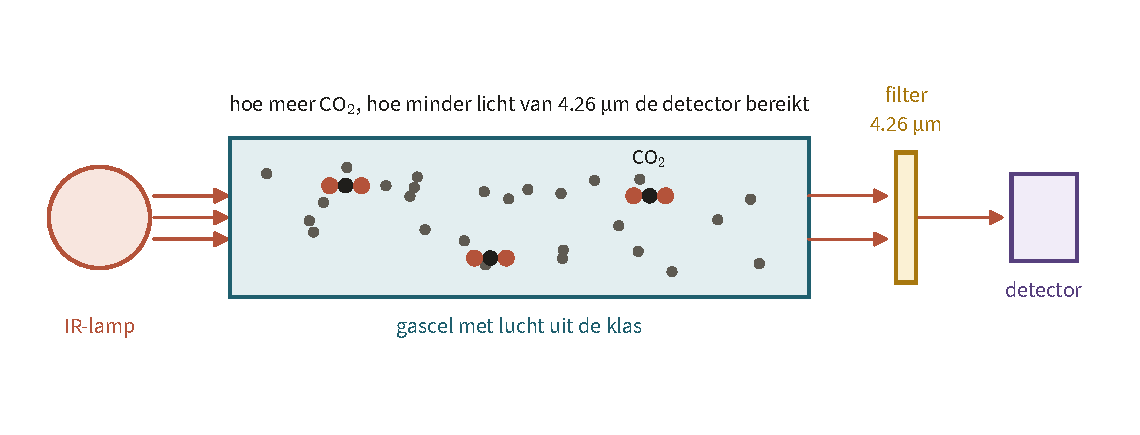
\includegraphics[width=0.85\linewidth]{Figuren/ndir_sensor}
    \caption{Principe van een CO$_2$-meter (niet-dispersieve infraroodsensor). Enkel CO$_2$ absorbeert het licht van \SI{4.26}{\micro\metre}; stikstof, zuurstof en argon, samen meer dan \SI{99.9}{\percent} van de lucht, laten het door.}
    \label{fig:ndir}
\end{figure}

Hetzelfde verschijnsel bepaalt het klimaat. Lucht bestaat voor \SI{78}{\percent} uit stikstof en voor \SI{21}{\percent} uit zuurstof, maar die gassen laten infrarood licht ongehinderd door. Het zijn sporengassen, vooral waterdamp en CO$_2$, die de warmtestraling van de aarde tegenhouden. Zonder hen zou de gemiddelde temperatuur aan het aardoppervlak ongeveer \SI{-18}{\celsius} zijn in plaats van \SI{15}{\celsius}.

Wie dit wil begrijpen, botst op vragen die de thermodynamica van hoofdstuk~\ref{ch:energie} niet kan beantwoorden:
\begin{itemize}
\item De zon straalt vooral zichtbaar licht uit, de aarde infrarood. Waar komt dat verschil vandaan, en wat kan elk soort straling met een molecule doen (\S\ref{sec:licht-pakketjes})?
\item Waarom absorbeert een gas enkel bij welbepaalde golflengten, zoals \SI{4.26}{\micro\metre}, en niet ertussen (\S\ref{sec:lijnenspectra})?
\item Stikstof is het hoofdbestanddeel van de lucht, en toch reageert het bijna nergens mee. Waarom is die molecule zo stabiel (\S\ref{sec:molecuulorbitalen})?
\item Waarom absorbeert CO$_2$ infrarood en stikstof niet, hoewel beide moleculen trillen (\S\ref{sec:moleculaire-beweging})?
\item Waarom heeft CO$_2$ een veel grotere warmtecapaciteit dan stikstof, en waarom stijgt die met de temperatuur (\S\ref{sec:kwantum-thermo})?
\end{itemize}
De antwoorden liggen op de schaal van atomen en moleculen. Daar blijkt energie niet continu maar \emph{gekwantiseerd}: enkel bepaalde waarden zijn toegelaten. Dat geldt voor de elektronen in een atoom, wat de chemische binding en de reactie-enthalpie verklaart, en voor de rotatie en de trilling van een molecule als geheel, wat de absorptie van infrarood en de warmtecapaciteit verklaart.

Net als in hoofdstuk~\ref{ch:energie} start elke sectie met een concreet probleem, bouwt ze de theorie op die nodig is om het op te lossen, en werkt ze het probleem op het einde uit. Het doel is geen volledige cursus kwantummechanica, maar de fundamenten die later terugkomen: de elektronenstructuur bepaalt hoe sterk een molecule aan een katalysator bindt (hoofdstuk~\ref{ch:grensvlakken}), de verdeling van moleculen over hun energieniveaus leidt naar de entropie (hoofdstuk~\ref{ch:spontaniteit}), en vibratie- en rotatieniveaus zijn de basis van de spectroscopie die je in latere vakken gebruikt.

\section{Licht komt in pakketjes}
\label{sec:licht-pakketjes}

\begin{casus}{zon en aarde}
De zon straalt vooral zichtbaar licht uit, de aarde vooral infrarood. We zoeken in deze sectie drie dingen:
\begin{enumerate}
\item bij welke golflengte de zon en de aarde het meest uitstralen, en waarom die zo verschillen;
\item hoeveel energie één foton van elk soort straling draagt, vergeleken met de energie van een chemische binding;
\item hoe warm de aarde zou zijn als haar atmosfeer geen infrarood tegenhield.
\end{enumerate}
\emph{Gegevens.} Het oppervlak van de zon is ongeveer \SI{5800}{\kelvin}, het aardoppervlak gemiddeld \SI{15}{\celsius} (\SI{288}{\kelvin}). Bij de aarde levert de zon \SI{1361}{\watt\per\metre\squared} op een vlak loodrecht op de stralen (de \emph{zonneconstante} $S$). De aarde weerkaatst \SI{30}{\percent} van dat licht. Een C--C-binding heeft een bindingsenergie van \SI{348}{\kilo\joule\per\mole}.

\emph{Schat eerst zelf:} heeft een foton zichtbaar licht meer of minder energie dan een foton infrarood? Kan zonlicht een binding breken? En zou de aarde zonder broeikasgassen warmer of kouder zijn dan nu, en ongeveer hoeveel?
\end{casus}

Rond 1900 leek de natuurkunde bijna af. De wetten van Newton, de thermodynamica en de elektromagnetische theorie van Maxwell verklaarden een enorm gebied aan verschijnselen. Toch bleven enkele waarnemingen onverklaarbaar. Volgens de klassieke fysica kan een atoom zelfs niet stabiel zijn: een elektron dat rond een kern draait, is een versnelde lading, zendt dus straling uit, verliest energie en zou binnen een fractie van een seconde al spiralerend in de kern storten. Drie experimenten toonden waar het misliep: de straling van een gloeiend voorwerp, het foto-elektrisch effect en de lijnenspectra van atomen. We bekijken ze een voor een. De klassieke fysica blijkt daarbij niet fout, maar een benadering die enkel voor grote voorwerpen geldt.

\subsection{Energie als discrete grootheid}

\paragraph{Het probleem: de kleur van een gloeiend voorwerp.}
Een metalen staaf die je verwarmt, gloeit eerst donkerrood, dan oranje, geel en uiteindelijk bijna wit. De kleur van het uitgezonden licht hangt dus rechtstreeks af van de temperatuur. Om dat te begrijpen, bestudeerden natuurkundigen een geïdealiseerd voorwerp dat alle invallende straling absorbeert en ze bij zijn eigen temperatuur weer uitzendt: een \emph{zwart lichaam}. In het labo maak je er een met een holle oven met een klein gaatje in de wand (figuur~\ref{fig:trillingsmodi}a). Licht dat door het gaatje binnenvalt, weerkaatst zo vaak op de wanden dat het nooit meer buitenkomt; wat uit het gaatje straalt, is zuiver de warmtestraling van de wanden. Het spectrum van die straling kon men rond 1900 zeer nauwkeurig meten. Het werd de toetssteen voor elke theorie.

\paragraph{Wat is een trillingsmodus?}
In de holte vormt het elektromagnetische veld golven die heen en weer weerkaatsen tussen de wanden. Een golf kan daar niet om het even hoe trillen. Net als een gitaarsnaar die aan beide uiteinden vastzit, moet de golf aan een geleidende wand nul zijn. Er passen dus enkel \emph{staande golven} met een geheel aantal halve golflengten tussen de wanden: $L = n\lambda/2$, met $n = 1, 2, 3, \ldots$ Elk zo'n toegelaten trillingspatroon heet een \emph{trillingsmodus} van het stralingsveld. Een modus is dus geen deeltje en geen atoom, maar een manier waarop het veld in de holte kan trillen, met een eigen golflengte en frequentie.

Hoe korter de golflengte, hoe meer manieren er zijn om een staande golf in de holte te passen. Op een snaar zie je dat al: tussen golflengte $2L$ en $L$ ligt één modus, maar tussen $2L/10$ en $L/10$ liggen er tien. In drie dimensies kan de golf bovendien in alle richtingen staan, en stijgt het aantal modi per frequentie-interval met $\nu^2$. Er zijn dus veel meer modi bij hoge dan bij lage frequenties.

\begin{figure}[htb]
    \centering
    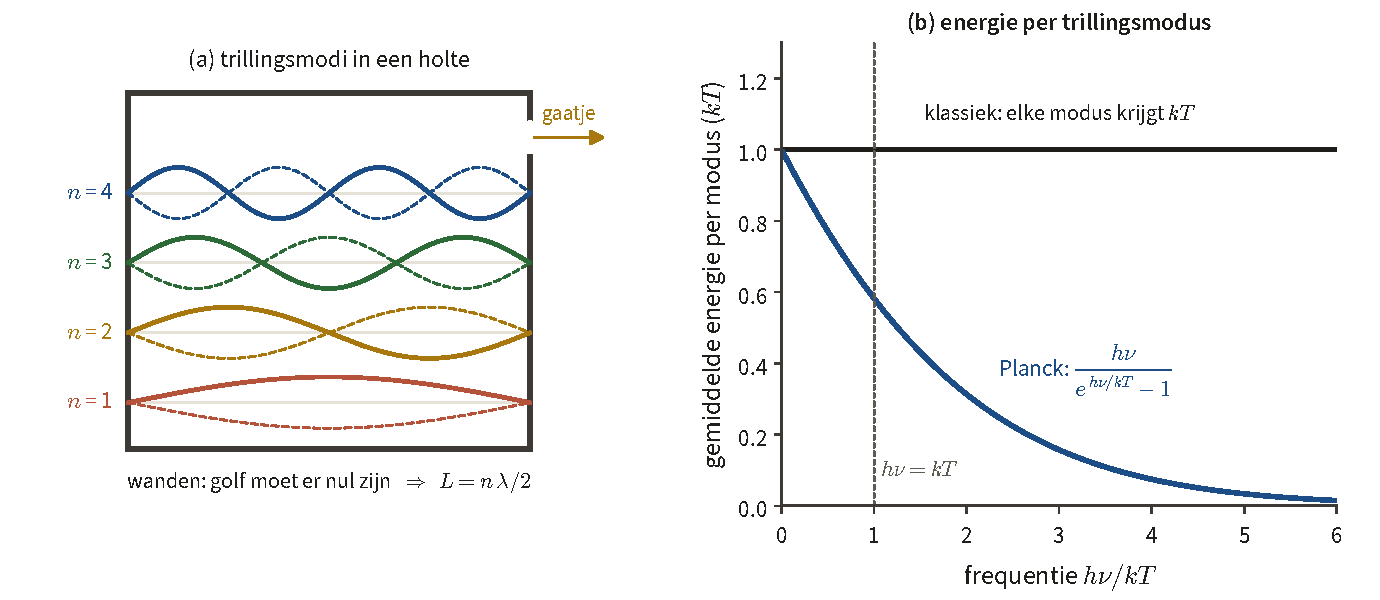
\includegraphics[width=0.95\linewidth]{Figuren/trillingsmodi}
    \caption{(a) Een zwart lichaam als holte met een gaatje. Tussen de wanden passen enkel staande golven met een geheel aantal halve golflengten: de trillingsmodi. (b) De gemiddelde energie per modus. Klassiek krijgt elke modus $kT$; volgens Planck daalt die energie sterk zodra $h\nu$ groter wordt dan $kT$.}
    \label{fig:trillingsmodi}
\end{figure}

\paragraph{De ultravioletcatastrofe.}
De klassieke statistische fysica kent aan elke trillingsmodus gemiddeld dezelfde energie $kT$ toe, net zoals ze dat doet voor elke vrijheidsgraad van een gasmolecule (de \emph{equipartitiestelling}). Het uitgestraalde vermogen bij een frequentie is dan evenredig met het aantal modi maal $kT$, dus met $\nu^2 kT$. Dat is de wet van Rayleigh en Jeans. Ze werkt goed bij lange golflengten, maar bij hoge frequenties stijgt ze zonder grens. Tel je alle modi op, dan zou een warm voorwerp een \emph{oneindige} hoeveelheid energie uitstralen, vooral in het ultraviolet. Dit werd de \emph{ultravioletcatastrofe} genoemd (figuur~\ref{fig:UVcatastrophe}). De metingen tonen het tegendeel: na een maximum daalt de intensiteit bij hoge frequenties sterk.

\begin{figure}[htb]
    \centering
    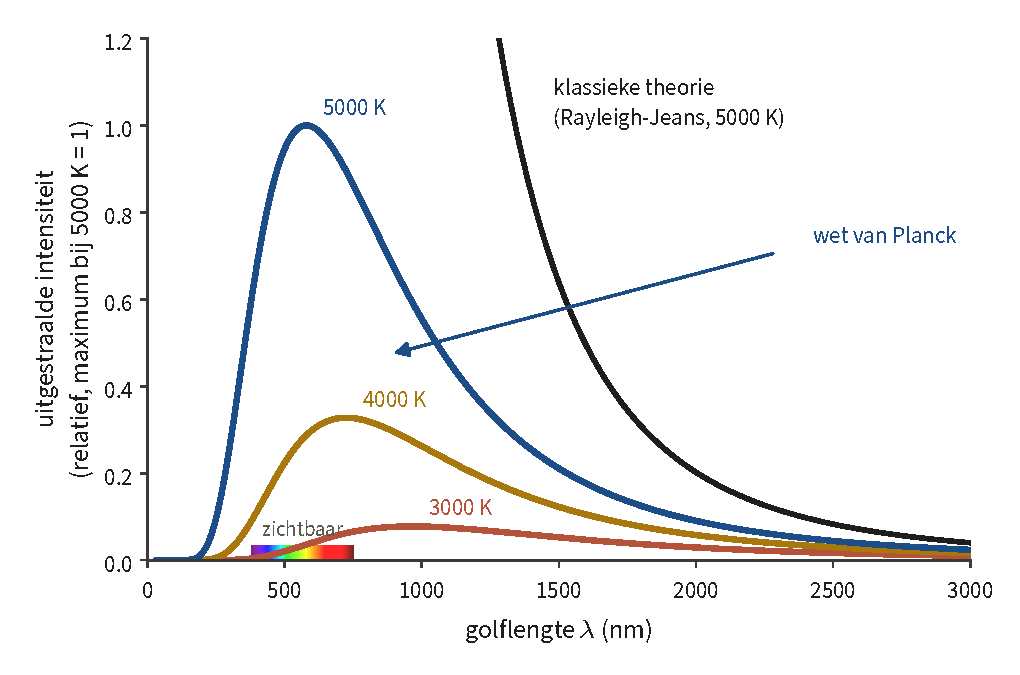
\includegraphics[width=0.62\linewidth]{Figuren/uv_catastrofe}
    \caption{Stralingsspectrum van een zwart lichaam. De wet van Rayleigh--Jeans (klassiek) loopt bij korte golflengten naar oneindig; de wet van Planck volgt de metingen.}
    \label{fig:UVcatastrophe}
\end{figure}

\paragraph{De oplossing van Planck.}
Max Planck loste dit in 1900 op met een gedurfde hypothese: een trillingsmodus met frequentie $\nu$ kan geen willekeurige hoeveelheid energie bevatten, maar enkel een geheel aantal ondeelbare pakketjes, \emph{kwanta}, van grootte
\begin{equation}
\boxed{
E=h\nu=h\frac{c}{\lambda}
}
\end{equation}
met $h=\SI{6.626e-34}{\joule\second}$ de constante van Planck, $\nu$ de frequentie, $\lambda$ de golflengte en $c$ de lichtsnelheid. Een modus bevat dus $0$, $h\nu$, $2h\nu$, \ldots, maar nooit $0.4\,h\nu$.

Waarom lost dat het probleem op? Bij temperatuur $T$ is de typische thermische energie die beschikbaar is van de orde $kT$. Voor een modus met lage frequentie is $h\nu \ll kT$: de pakketjes zijn klein, de energie lijkt continu, en de modus krijgt zoals klassiek ongeveer $kT$. Voor een modus met hoge frequentie is $h\nu \gg kT$: zelfs één pakketje is al te groot om met de beschikbare thermische energie te leveren, en de modus blijft meestal leeg. Planck vond dat de gemiddelde energie per modus gelijk is aan $h\nu/(e^{h\nu/kT}-1)$ (figuur~\ref{fig:trillingsmodi}b). Die uitdrukking volgt uit de Boltzmannverdeling, die we in \S\ref{sec:kwantum-thermo} uitwerken. Vermenigvuldig je ze met het aantal modi, dan krijg je het uitgestraalde vermogen per oppervlakte en per golflengte-interval, de \emph{wet van Planck}:
\begin{equation}
M_\lambda(T) = \frac{2\pi h c^2}{\lambda^5}\,\frac{1}{e^{hc/(\lambda k T)}-1}.
\label{eq:planck}
\end{equation}
Die formule beschrijft het gemeten spectrum bij elke temperatuur. Planck zag zijn kwanta aanvankelijk als een rekentruc, maar ze bleken een fundamentele eigenschap van de natuur. Op macroscopische schaal zijn de kwanta zo klein dat energie continu \emph{lijkt}; op atomaire schaal bepalen ze het gedrag van materie.

\paragraph{Twee gevolgen: de wetten van Wien en van Stefan--Boltzmann.}
Wat betekent de wet van Planck voor de gloeiende staaf? Figuur~\ref{fig:gloeiende-staaf}a toont het spectrum bij \SI{1000}{}, \SI{1250}{} en \SI{1500}{\kelvin}. Twee zaken vallen op, en elk ervan is een wet die je in de techniek voortdurend gebruikt.

\begin{figure}[htb]
    \centering
    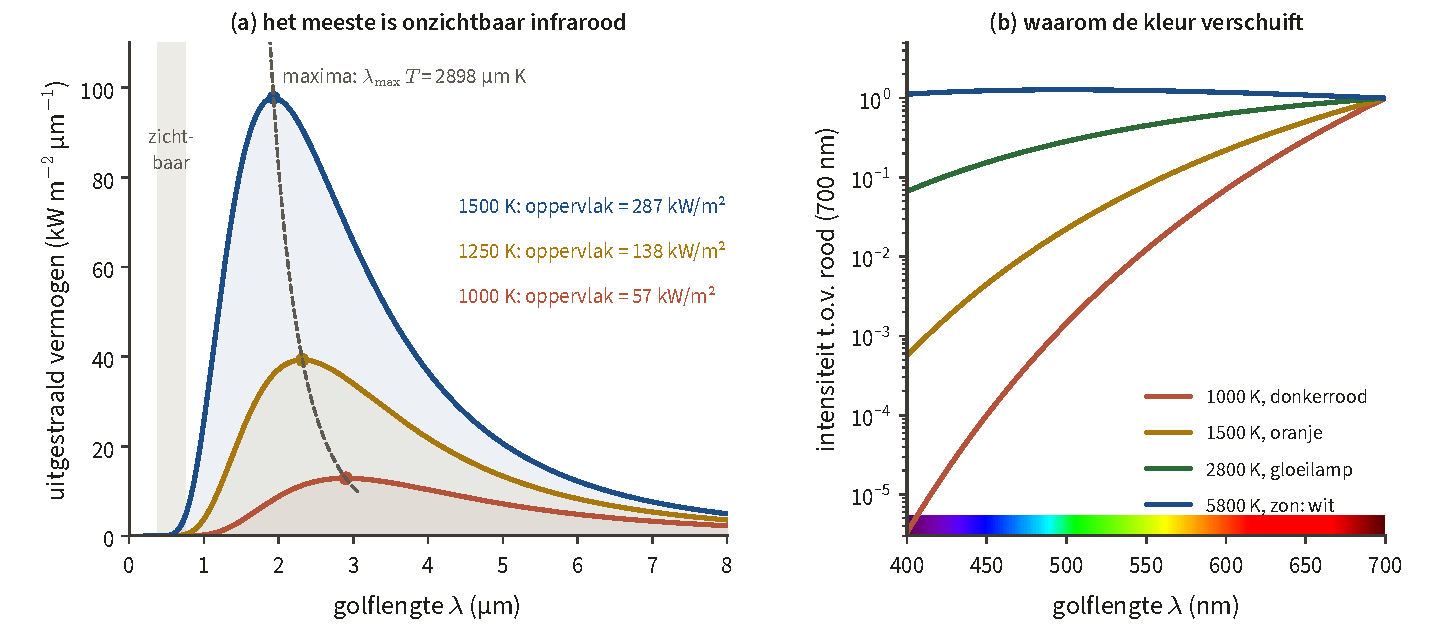
\includegraphics[width=\linewidth]{Figuren/gloeiende_staaf}
    \caption{(a) Straling van een gloeiende staaf volgens de wet van Planck. Het maximum schuift naar kortere golflengten als de temperatuur stijgt (wet van Wien, stippellijn), en het oppervlak onder de kromme, het totale vermogen, stijgt met $T^4$ (wet van Stefan--Boltzmann). Bijna alle straling is onzichtbaar infrarood. (b) Het zichtbare deel, relatief ten opzichte van rood licht. Bij \SI{1000}{\kelvin} is blauw honderdduizend keer zwakker dan rood: de staaf gloeit donkerrood. Bij hogere temperatuur wordt het spectrum in het zichtbare vlakker en het licht witter.}
    \label{fig:gloeiende-staaf}
\end{figure}

Ten eerste schuift het maximum naar kortere golflengten naarmate het voorwerp warmer is. Zoek je het maximum van~\eqref{eq:planck} door de afgeleide naar $\lambda$ nul te stellen, dan vind je dat het product van de golflengte van het maximum en de temperatuur een constante is, de \emph{verschuivingswet van Wien}:
\begin{equation}
\lambda_{\max}\,T = \SI{2898}{\micro\metre\kelvin}.
\label{eq:wien}
\end{equation}
De betekenis is eenvoudig: \emph{de kleur van de straling is een thermometer}. Voor de staaf bij \SI{1000}{\kelvin} ligt het maximum bij \SI{2.9}{\micro\metre}, ver in het infrarood. Slechts een miljoenste van de straling valt in het zichtbare gebied, en dat is het uiterste rode staartje van het spectrum: de staaf gloeit donkerrood, maar vooral voel je zijn warmte. Wordt de staaf warmer, dan schuift de hele kromme naar links, en komt er naast rood steeds meer oranje, geel en blauw licht bij (figuur~\ref{fig:gloeiende-staaf}b). Bij ongeveer \SI{2800}{\kelvin}, de gloeidraad van een klassieke gloeilamp, is het licht bijna wit, maar ligt het maximum nog steeds in het infrarood (\SI{1.0}{\micro\metre}): slechts ongeveer \SI{8}{\percent} van het vermogen is zichtbaar licht. Daarom zijn gloeilampen vervangen door ledlampen.

Ten tweede wordt het oppervlak onder de kromme veel groter. Dat oppervlak is het totale uitgestraalde vermogen per oppervlakte. Integreer je~\eqref{eq:planck} over alle golflengten, dan vind je de \emph{wet van Stefan--Boltzmann}:
\begin{equation}
\frac{P}{A} = \sigma T^4, \qquad \sigma = \SI{5.67e-8}{\watt\per\metre\squared\per\kelvin\tothe{4}}.
\label{eq:stefan-boltzmann}
\end{equation}
Ook hier is de betekenis direct bruikbaar: \emph{het stralingsverlies stijgt met de vierde macht van de temperatuur}. Van \SI{1000}{} naar \SI{1500}{\kelvin} stijgt de temperatuur met de helft, maar de uitstraling met een factor $1.5^4 = 5.1$. Bij kamertemperatuur is straling een bescheiden vorm van warmteoverdracht; in een oven of in de vuurhaard van een stoomketel is ze dominant. Een echt oppervlak straalt minder dan een zwart lichaam, $P/A = \varepsilon\sigma T^4$, met een \emph{emissiviteit} $\varepsilon$ tussen 0 en 1: ongeveer 0.05 voor blank gepolijst metaal, 0.8 tot 0.9 voor geoxideerd staal, baksteen en de menselijke huid.

Beide wetten gebruik je meer dan je denkt. Een thermische camera of oorthermometer meet het infrarood rond \SI{10}{\micro\metre}: volgens~\eqref{eq:wien} straalt een mens van \SI{310}{\kelvin} het sterkst bij \SI{9.3}{\micro\metre}. Een pyrometer meet de temperatuur van gesmolten staal of van een ovenwand zonder contact, uit de intensiteit of de kleur van de straling. En de isolatie van ovens en stoomleidingen wordt berekend met~\eqref{eq:stefan-boltzmann}.

\begin{voorbeeld}{Hoeveel straalt een gloeiende staaf uit?}
Een stalen staaf met diameter \SI{2.0}{\centi\metre} en lengte \SI{30}{\centi\metre} ($\varepsilon = 0.80$) wordt in een smidse verhit tot \SI{1000}{\kelvin}. Het zijoppervlak is $A = \pi d L = \pi(0.020)(0.30) = \SI{0.0188}{\metre\squared}$. De staaf straalt
\[
P = \varepsilon\sigma T^4 A = (0.80)(5.67\times10^{-8})(1000)^4(0.0188) = \SI{855}{\watt}
\]
uit, ongeveer evenveel als een waterkoker op halve kracht. De omgeving van \SI{300}{\kelvin} straalt terug met $(300/1000)^4 = \SI{0.8}{\percent}$ daarvan, wat verwaarloosbaar is. Bij \SI{1500}{\kelvin} wordt dat $855 \times 5.06 = \SI{4.3}{\kilo\watt}$. Om een staaf op hoge temperatuur te houden, moet de smid dus steeds sneller warmte toevoeren.
\end{voorbeeld}

\begin{figure}[htb]
    \centering
    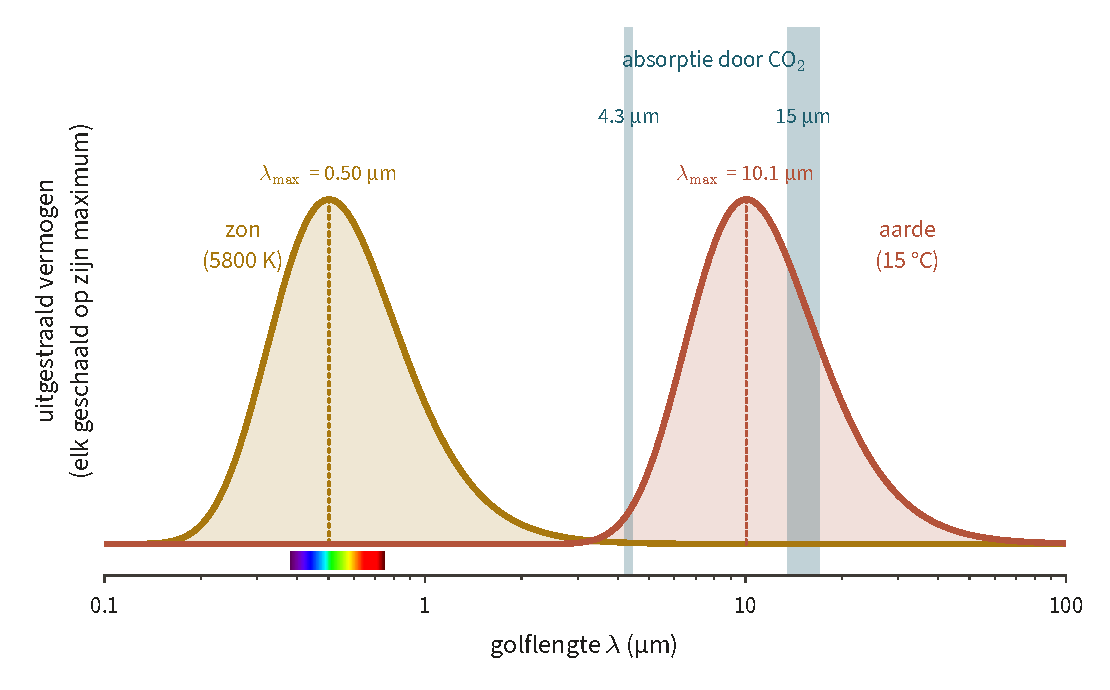
\includegraphics[width=0.8\linewidth]{Figuren/zon_aarde_spectrum}
    \caption{Straling van de zon (oppervlak \SI{5800}{\kelvin}) en van de aarde (\SI{15}{\celsius}) volgens de wet van Planck, elk geschaald op zijn maximum. De twee spectra overlappen nauwelijks. De gekleurde banden zijn de sterkste absorptiebanden van CO$_2$: ze vallen in het infrarood van de aarde, niet in het zonlicht.}
    \label{fig:zon-aarde}
\end{figure}

\paragraph{De energie van één foton.}
Om een gevoel te krijgen voor de grootte van $E=h\nu$, vergelijken we drie soorten straling.

\begin{voorbeeld}{Fotonenergie over het elektromagnetisch spectrum}
Met $E=hc/\lambda$ en $c=\SI{3.00e8}{\meter\per\second}$:
\begin{align*}
E_{\text{radio}} &= \frac{(6.626\times10^{-34})(3.00\times10^{8})}{3} = \SI{6.63e-26}{\joule} \quad (\lambda=\SI{3}{\meter}) \\
E_{\text{groen}} &= \frac{(6.626\times10^{-34})(3.00\times10^{8})}{520\times10^{-9}} = \SI{3.82e-19}{\joule} \quad (\lambda=\SI{520}{\nano\meter}) \\
E_{\text{X}} &= \frac{(6.626\times10^{-34})(3.00\times10^{8})}{0.1\times10^{-9}} = \SI{1.99e-15}{\joule} \quad (\lambda=\SI{0.1}{\nano\meter})
\end{align*}
Tussen radio en röntgen zit een factor $10^{10}$, hoewel beide ``gewoon'' elektromagnetische straling zijn. Radiogolven zijn daarom onschadelijk voor chemische bindingen, terwijl UV- en röntgenfotonen bindingen kunnen breken of elektronen kunnen losmaken: hun energie ligt in dezelfde grootteorde als elektronische energieverschillen (figuur~\ref{fig:spectrum-bindingen}).
\end{voorbeeld}

\begin{figure}[htb]
    \centering
    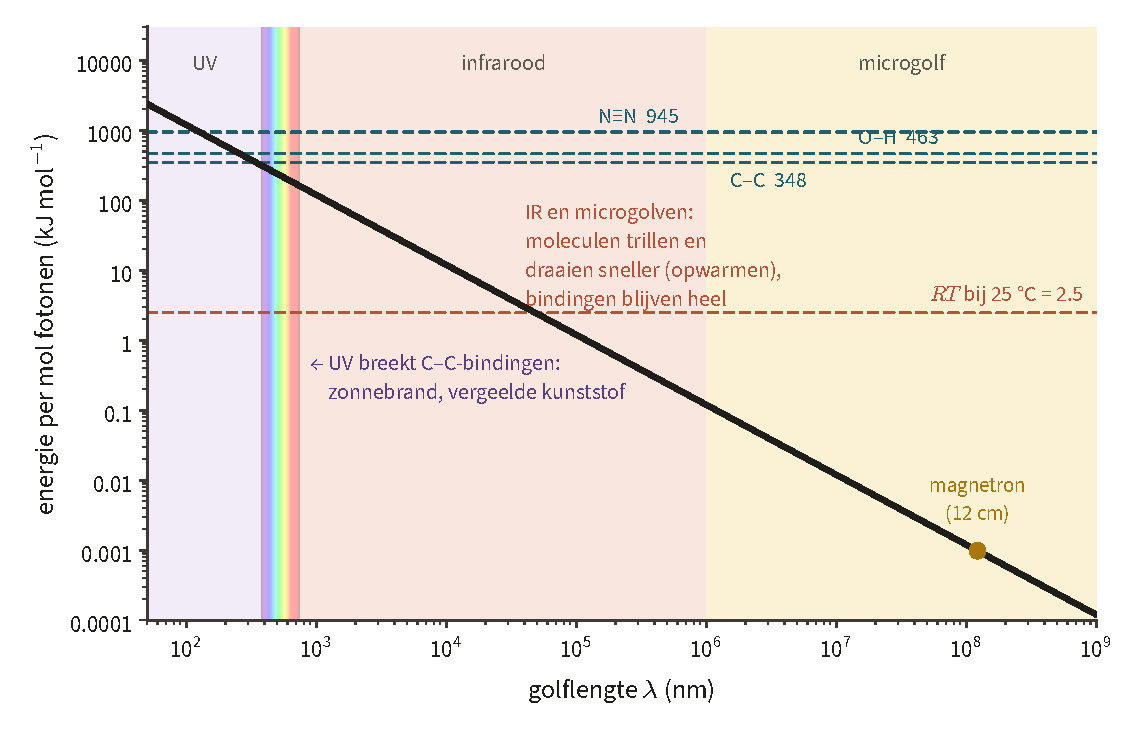
\includegraphics[width=0.62\linewidth]{Figuren/spectrum_bindingen}
    \caption{Energie van één mol fotonen over het elektromagnetisch spectrum, vergeleken met enkele bindingsenergieën en met $RT$ bij kamertemperatuur. Ultraviolet licht kan C--C-bindingen breken (zonnebrand, vergeelde kunststof); infrarood en microgolven doen moleculen enkel sneller trillen en draaien.}
    \label{fig:spectrum-bindingen}
\end{figure}

\subsection{Het foto-elektrisch effect}

\paragraph{Het experiment.}
Planck had de kwanta ingevoerd voor de uitwisseling van energie tussen materie en straling. Of het licht zelf uit pakketjes bestaat, bleef open. Het antwoord kwam uit een experiment dat Heinrich Hertz in 1887 bij toeval opmerkte: een vonk sprong gemakkelijker over wanneer de elektroden met ultraviolet licht werden beschenen. Philipp Lenard onderzocht het effect rond 1902 systematisch met de opstelling van figuur~\ref{fig:foto-opstelling}a. In een vacuümbuis staan twee elektroden: een metalen plaat en een collector. Licht valt door een kwartsvenster, dat ook UV doorlaat, op de plaat. Maakt het licht elektronen vrij, dan vliegen sommige naar de collector en meet een ampèremeter in de uitwendige kring een stroom.

Met een regelbare spanning kun je de collector ook negatief maken ten opzichte van de plaat. Die \emph{tegenspanning} $U$ remt de elektronen af: enkel elektronen met een kinetische energie groter dan $eU$ bereiken de collector nog. Bij een bepaalde \emph{stopspanning} $U_s$ valt de stroom volledig weg. Ook het snelste elektron haalt de collector dan net niet, zodat
\[
E_{\mathrm{kin,max}} = eU_s .
\]
Zo meet je met een eenvoudige voltmeter de maximale energie van de vrijgemaakte elektronen. Lenard varieerde vervolgens de intensiteit en de frequentie (de kleur) van het licht.

\begin{figure}[htb]
    \centering
    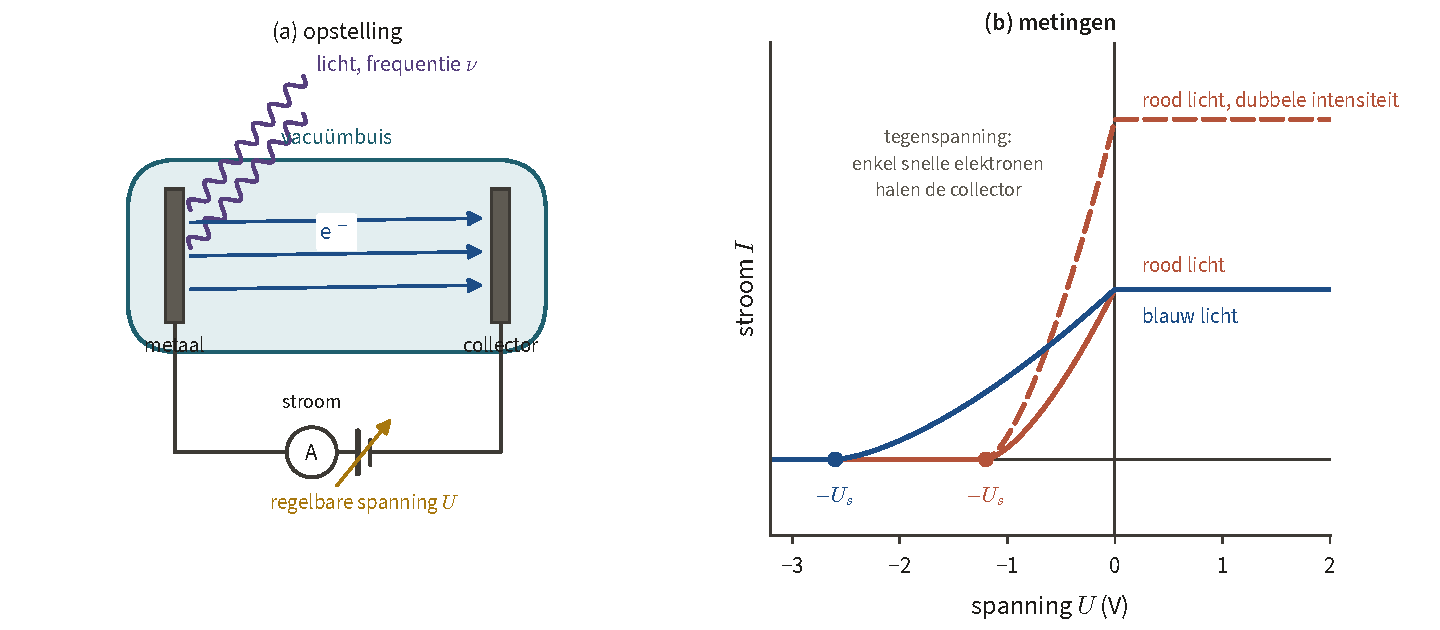
\includegraphics[width=\linewidth]{Figuren/foto_opstelling}
    \caption{(a) Opstelling voor het foto-elektrisch effect. Licht maakt elektronen vrij uit een metalen plaat; met een tegenspanning $U$ wordt gemeten hoe snel ze zijn. (b) Stroom tegen spanning. Dubbel zoveel licht van dezelfde kleur geeft een dubbele stroom, maar dezelfde stopspanning $U_s$. Licht met een hogere frequentie geeft een grotere stopspanning, dus snellere elektronen.}
    \label{fig:foto-opstelling}
\end{figure}

\paragraph{De waarnemingen.}
Volgens de klassieke golftheorie draagt een lichtgolf haar energie continu, evenredig met haar intensiteit. Intenser licht zou de elektronen dus sneller moeten maken, en bij zwak licht zou het even moeten duren voor een elektron genoeg energie heeft opgestapeld. De metingen (figuur~\ref{fig:foto-opstelling}b) toonden iets heel anders:
\begin{enumerate}
\item Onder een \emph{drempelfrequentie} $\nu_0$ komt geen enkel elektron vrij, hoe intens het licht ook is. Rood licht maakt uit zink geen elektronen vrij, ook niet met een sterke lamp; zwak UV-licht doet dat wel.
\item Boven de drempel komen de elektronen \emph{onmiddellijk} vrij, ook bij zeer zwak licht. Er is geen opstapeltijd.
\item Meer licht van dezelfde kleur geeft \emph{meer} elektronen (een grotere stroom), maar niet \emph{snellere}: de stopspanning blijft dezelfde. De maximale kinetische energie hangt enkel af van de frequentie.
\end{enumerate}

\paragraph{De verklaring van Einstein.}
In 1905 stelde Einstein dat licht zelf uit energiepakketjes bestaat, later \emph{fotonen} genoemd, elk met energie $h\nu$. Eén elektron absorbeert telkens één volledig foton. Een deel van die energie, de \emph{werkfunctie} $\Phi$, is nodig om het elektron uit het metaal te halen; de rest wordt kinetische energie (figuur~\ref{fig:photoelectric}):
\begin{equation}
h\nu = \Phi + E_{\mathrm{kin,max}}
\qquad\text{of}\qquad
\boxed{E_{\mathrm{kin,max}} = \tfrac{1}{2}m_ev^2 = h\nu-\Phi .}
\end{equation}
De drie waarnemingen volgen er meteen uit. Is $h\nu < \Phi$, dan kan geen enkel foton een elektron vrijmaken, hoeveel fotonen er ook zijn (waarneming 1). Is $h\nu > \Phi$, dan gebeurt het bij de eerste absorptie (waarneming 2). Intenser licht betekent meer fotonen, dus meer elektronen, maar elk foton heeft nog steeds dezelfde energie (waarneming 3). De drempelfrequentie is $\nu_0 = \Phi/h$.

\begin{figure}[htb]
    \centering
    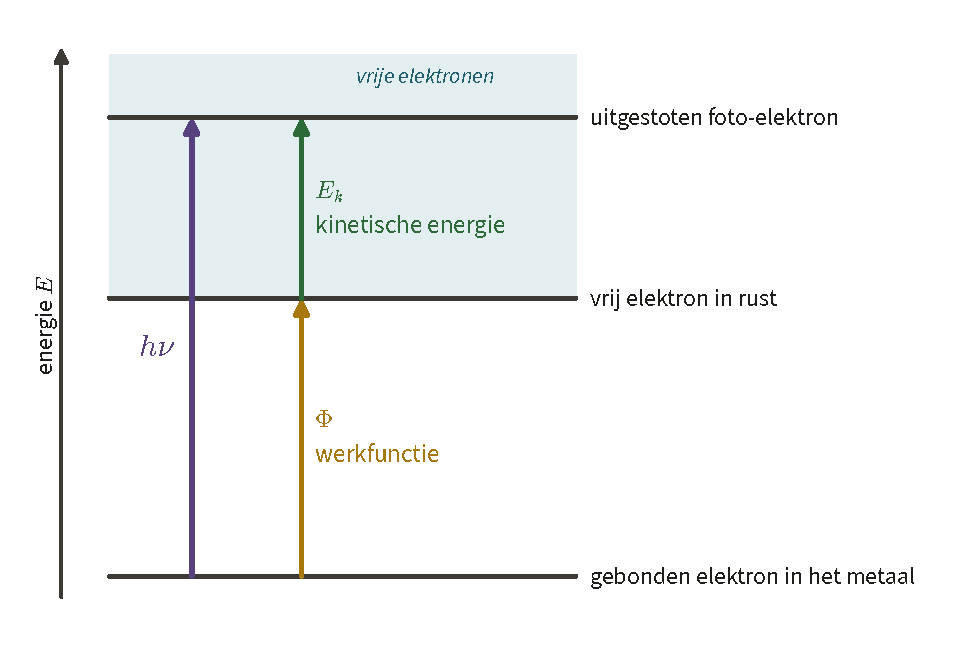
\includegraphics[width=0.55\linewidth]{Figuren/foto_elektrisch}
    \caption{Een foton met energie $h\nu$ maakt een elektron vrij: een deel van de energie dient om het metaal te verlaten ($\Phi$), de rest wordt kinetische energie ($E_k$).}
    \label{fig:photoelectric}
\end{figure}

Robert Millikan, die Einstein aanvankelijk wilde weerleggen, mat in 1916 de stopspanning bij veel frequenties en voor verschillende metalen. Hij vond rechte lijnen met voor elk metaal dezelfde helling $h$ (figuur~\ref{fig:ek-frequentie}), en bepaalde zo de constante van Planck tot op een half procent nauwkeurig.

\begin{figure}[htb]
    \centering
    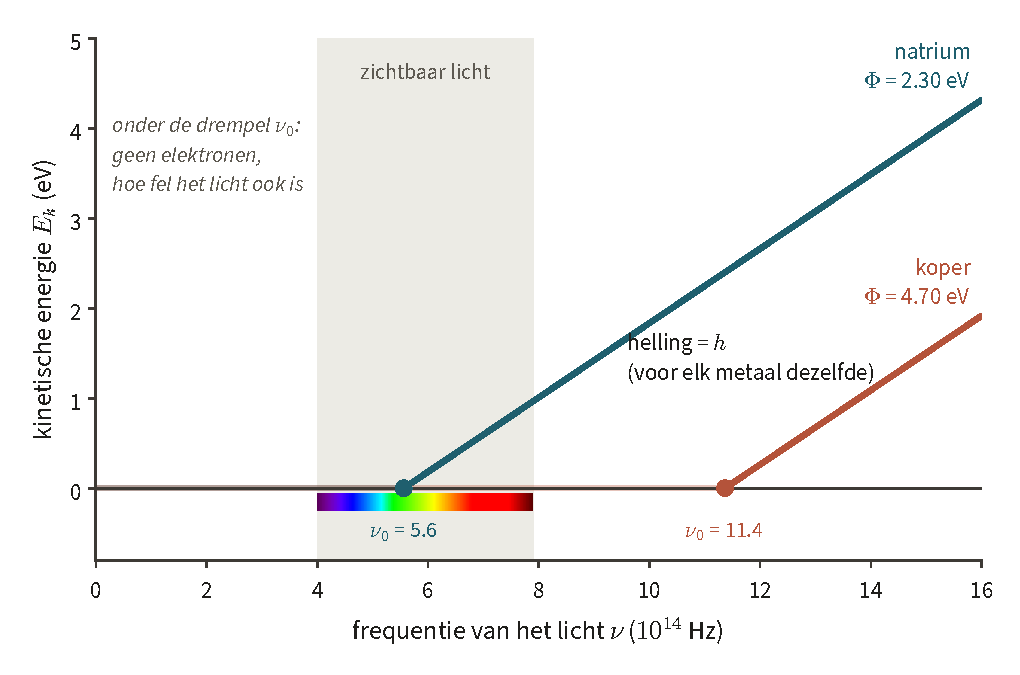
\includegraphics[width=0.6\linewidth]{Figuren/ek_frequentie}
    \caption{Maximale kinetische energie van de uitgestoten elektronen tegen de frequentie, voor natrium en koper. Onder $\nu_0 = \Phi/h$ komen geen elektronen vrij; daarboven stijgt $E_{\mathrm{kin,max}}$ lineair met helling $h$, voor elk metaal dezelfde.}
    \label{fig:ek-frequentie}
\end{figure}

Energieën op deze schaal druk je handig uit in \emph{elektronvolt}: $\SI{1}{\electronvolt}=\SI{1.602e-19}{\joule}$ is de energie die één elektron krijgt bij een spanningsverschil van \SI{1}{\volt}. Een stopspanning van \SI{2.66}{\volt} betekent dus een maximale kinetische energie van \SI{2.66}{\electronvolt}. Typische werkfuncties liggen tussen \SI{2}{} en \SI{5}{\electronvolt}.

\begin{voorbeeld}{Foto-elektrisch effect}
Natrium ($\Phi=\SI{2.30}{eV}$) wordt bestraald met UV-licht van \SI{250}{nm}. Eén foton heeft
\[
E=\frac{hc}{\lambda}=\frac{(6.626\times10^{-34})(3.00\times10^{8})}{250\times10^{-9}}=\SI{7.95e-19}{J}=\SI{4.96}{eV},
\]
zodat $E_{\mathrm{kin,max}}=4.96-2.30=\SI{2.66}{eV}$. In de opstelling van figuur~\ref{fig:foto-opstelling} is een tegenspanning van \SI{2.66}{\volt} nodig om de stroom te stoppen. De drempelgolflengte van natrium is $\lambda_0 = hc/\Phi = \SI{539}{\nano\metre}$: groen licht maakt nog net elektronen vrij, rood licht niet.
\end{voorbeeld}

De werkfunctie mag je niet verwarren met de ionisatie-energie. De werkfunctie is de energie om een elektron uit een vast metaal te halen; dat elektron bewoog al vrij door het metaal en moet enkel het oppervlak verlaten. De ionisatie-energie is de energie om een elektron volledig los te maken van één vrij atoom, tegen de volle aantrekking van de kern in. Voor natrium is de werkfunctie \SI{2.3}{\electronvolt}, de eerste ionisatie-energie \SI{5.1}{\electronvolt}.

Het foto-elektrisch effect is ook technisch belangrijk. Een fotocel of lichtsensor werkt op dit principe, en een zonnecel is er een variant van: daar wordt het elektron niet uit het materiaal gestoten, maar naar een hogere energieband gebracht, waar het als stroom kan wegvloeien. Ook dan geldt de drempel: silicium reageert enkel op fotonen boven ongeveer \SI{1.1}{\electronvolt}, dus golflengten korter dan \SI{1.1}{\micro\metre}.

\begin{casusuitgewerkt}{zon en aarde}
\emph{Stap 1: waar stralen zon en aarde het meest?} Met de wet van Wien~\eqref{eq:wien}:
\[
\lambda_{\max,\text{zon}} = \frac{\SI{2898}{\micro\metre\kelvin}}{\SI{5800}{\kelvin}} = \SI{0.50}{\micro\metre}, \qquad
\lambda_{\max,\text{aarde}} = \frac{\SI{2898}{\micro\metre\kelvin}}{\SI{288}{\kelvin}} = \SI{10.1}{\micro\metre}.
\]
De zon straalt het meest in het groen, de aarde in het verre infrarood (figuur~\ref{fig:zon-aarde}). Het verschil komt enkel van de temperatuur: zon en aarde zijn allebei, bij benadering, zwarte lichamen.

Waarom \SI{5800}{\kelvin}? De zon heeft geen vast oppervlak. Het licht dat ons bereikt, ontsnapt uit een laag van enkele honderden kilometer dik, de \emph{fotosfeer}, en die heeft ongeveer \SI{5800}{\kelvin}. Dieper in de zon is het veel heter (in de kern ongeveer 15~miljoen kelvin), en de ijle corona erboven haalt zelfs 1 tot 2~miljoen kelvin, maar straalt door haar lage dichtheid nauwelijks. Je kunt de \SI{5800}{\kelvin} zelf controleren met de wet van Stefan--Boltzmann. De zon straalt in totaal \SI{3.83e26}{\watt} uit over een bol met straal \SI{6.96e8}{\metre}:
\[
T = \left(\frac{P}{4\pi R^2\sigma}\right)^{1/4} = \left(\frac{3.83\times10^{26}}{4\pi(6.96\times10^{8})^2(5.67\times10^{-8})}\right)^{1/4} = \SI{5770}{\kelvin}.
\]

\emph{Stap 2: de energie per foton.} Per mol fotonen is $E_\mathrm{m} = N_\mathrm{A}hc/\lambda$:
\[
E_\mathrm{m}(\SI{0.50}{\micro\metre}) = \SI{239}{\kilo\joule\per\mole}, \qquad
E_\mathrm{m}(\SI{10}{\micro\metre}) = \SI{12}{\kilo\joule\per\mole}.
\]
Zichtbaar licht komt in de buurt van bindingsenergieën; UV-licht ($\lambda < \SI{0.35}{\micro\metre}$, meer dan \SI{340}{\kilo\joule\per\mole}) gaat erover en kan C--C-bindingen breken. Een infraroodfoton van de aarde heeft dertig keer te weinig energie om een binding te breken. Het kan een molecule enkel sneller laten trillen of draaien (figuur~\ref{fig:spectrum-bindingen}).

\emph{Stap 3: hoe koud zou de aarde zijn zonder broeikasgassen?} We stellen een energiebalans op voor de aarde als geheel (figuur~\ref{fig:stralingsbalans}). In evenwicht is wat binnenkomt gelijk aan wat buitengaat.
\begin{itemize}
\item \emph{In.} De zonnestralen vallen evenwijdig in. De aarde onderschept er evenveel van als een platte schijf met dezelfde straal: haar schaduw is een cirkel met oppervlak $\pi r^2$. Daarvan wordt \SI{30}{\percent} weerkaatst door wolken, ijs en woestijnen. Er wordt dus $(1-0.30)\,S\,\pi r^2$ geabsorbeerd.
\item \emph{Uit.} De aarde draait en houdt haar warmte vast, zodat ze dag en nacht en over haar volledige boloppervlak $4\pi r^2$ infrarood uitstraalt: $\sigma T^4 \cdot 4\pi r^2$.
\end{itemize}
Gelijkstellen geeft
\[
\sigma T^4 \cdot 4\pi r^2 = (1-0.30)\,S\,\pi r^2
\quad\Longrightarrow\quad
\sigma T^4 = \frac{(1-0.30)(1361)}{4} = \SI{238}{\watt\per\metre\squared}.
\]
De straal van de aarde valt weg; de factor 4 is de verhouding tussen het oppervlak van een bol en dat van zijn schaduw. Dan is
\[
T = \left(\frac{238}{5.67\times10^{-8}}\right)^{1/4} = \SI{255}{\kelvin} = \SI{-18}{\celsius}.
\]
De werkelijke gemiddelde temperatuur is \SI{15}{\celsius}. Het verschil van \SI{33}{\kelvin} is het natuurlijke broeikaseffect: een deel van het infrarood van de aarde wordt in de atmosfeer geabsorbeerd en gedeeltelijk teruggestraald naar het oppervlak, dat daardoor warmer moet worden om evenveel kwijt te raken.

\emph{Volgende vraag.} Figuur~\ref{fig:zon-aarde} toont dat CO$_2$ niet het hele infrarood absorbeert, maar enkel smalle banden rond \SI{4.3}{} en \SI{15}{\micro\metre}. Waarom absorbeert een gas enkel bij welbepaalde golflengten?
\end{casusuitgewerkt}

\begin{figure}[htb]
    \centering
    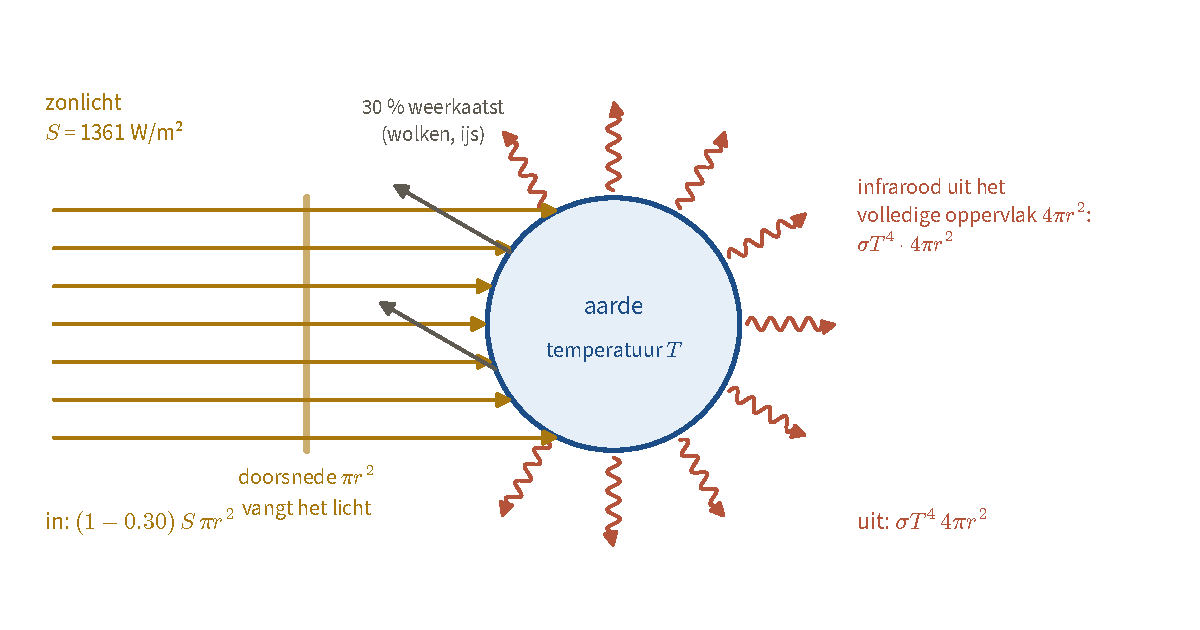
\includegraphics[width=0.85\linewidth]{Figuren/stralingsbalans_aarde}
    \caption{Stralingsbalans van de aarde. Het zonlicht wordt opgevangen door de doorsnede $\pi r^2$; \SI{30}{\percent} wordt weerkaatst. De aarde straalt infrarood uit over haar volledige oppervlak $4\pi r^2$.}
    \label{fig:stralingsbalans}
\end{figure}

\section{Discrete energieniveaus en lijnenspectra}
\label{sec:lijnenspectra}

\begin{casus}{scherpe lijnen}
De CO$_2$-meter van figuur~\ref{fig:ndir} gebruikt een filter van \SI{4.26}{\micro\metre}. Bij \SI{4.0}{} of \SI{4.6}{\micro\metre} zou hij niets meten: daar absorbeert CO$_2$ niet. Een gas absorbeert dus niet geleidelijk over het hele spectrum, maar bij scherpe golflengten. Hoe kan dat, en welke energie hoort bij \SI{4.26}{\micro\metre}?

\emph{Schat eerst zelf:} als een molecule enkel bepaalde energieën kan hebben, wat betekent dat voor de fotonen die ze kan opnemen?
\end{casus}

\subsection{Het model van Bohr}
\label{sec:bohr}

\paragraph{De waarneming: het lijnenspectrum van waterstof.}
Stuur je een elektrische ontlading door een buis met waterstofgas, dan splitst de ontlading de \ce{H2}-moleculen in atomen en geeft ze die atomen extra energie. De buis licht roze-paars op. Laat je dat licht door een smalle spleet en een prisma of tralie vallen (figuur~\ref{fig:waterstof-opstelling}), dan zie je geen doorlopende regenboog zoals bij een gloeiende staaf, maar slechts vier scherpe gekleurde lijnen: bij \SI{656}{} (rood), \SI{486}{} (blauwgroen), \SI{434}{} en \SI{410}{\nano\metre} (violet). Dit is een \emph{lijnenspectrum}, en elk element heeft er een eigen.

\begin{figure}[htb]
    \centering
    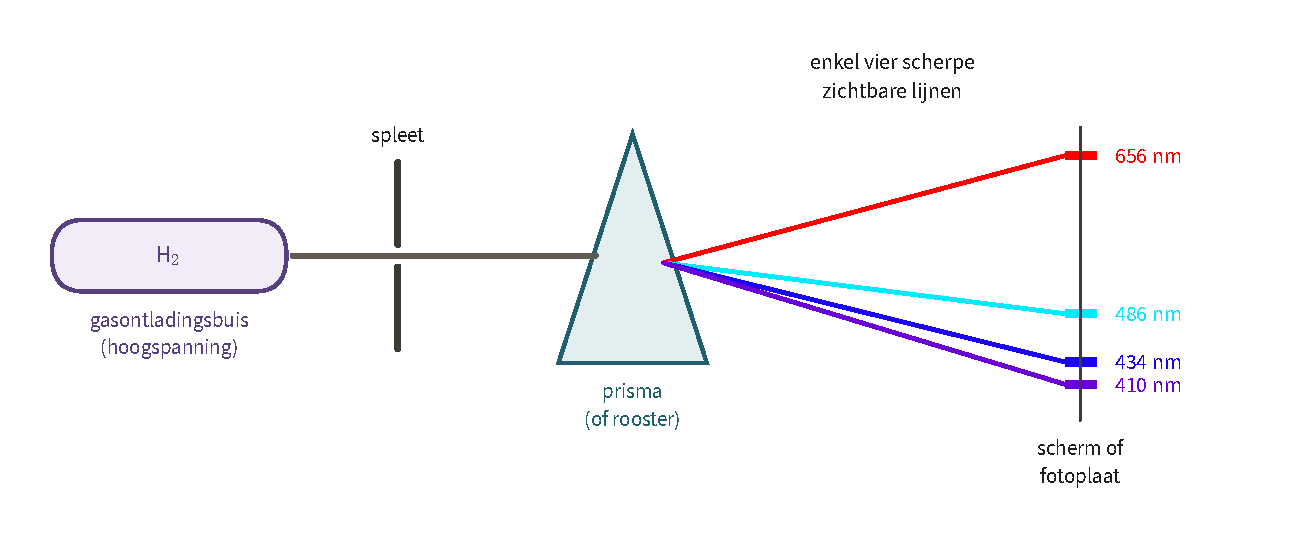
\includegraphics[width=0.9\linewidth]{Figuren/waterstof_opstelling}
    \caption{Het lijnenspectrum van waterstof. Het licht van een gasontladingsbuis wordt na een spleet door een prisma (of tralie) uitgesplitst. Op het scherm verschijnen enkel vier scherpe zichtbare lijnen.}
    \label{fig:waterstof-opstelling}
\end{figure}

In 1885 merkte de Zwitserse leraar Johann Balmer op dat de vier golflengten passen in een eenvoudige formule, $\lambda = B\,n^2/(n^2-4)$ met $B = \SI{364.6}{\nano\metre}$ en $n = 3, 4, 5, 6$. Probeer maar: $n=3$ geeft $364.6 \times 9/5 = \SI{656}{\nano\metre}$. Rydberg schreef dit later om tot
\[
\frac{1}{\lambda} = R_H\left(\frac{1}{2^2} - \frac{1}{n^2}\right), \qquad R_H = \SI{1.097e7}{\per\metre},
\]
en voorspelde dat er ook reeksen met $1/1^2$ en $1/3^2$ moesten bestaan. Die werden later gevonden in het ultraviolet (Lyman) en het infrarood (Paschen). De formule werkte perfect, maar niemand wist waarom. Waarom zendt waterstof enkel deze golflengten uit, en waarom zijn ze te schrijven als een verschil van twee termen $1/n^2$?

\paragraph{De postulaten van Bohr.}
Niels Bohr gaf in 1913 het eerste antwoord. Hij hield het klassieke beeld van een elektron dat op een cirkelbaan rond de kern draait, vastgehouden door de Coulombaantrekking, maar voegde er twee niet-klassieke postulaten aan toe:
\begin{enumerate}
\item Enkel banen waarvoor het impulsmoment een geheel veelvoud is van $\hbar = h/2\pi$ zijn toegelaten:
\begin{equation}
m_e v r = n\hbar, \qquad n=1,2,3,\ldots
\label{eq:bohr-kwantisatie}
\end{equation}
Op zo'n baan straalt het elektron, in strijd met de klassieke fysica, \emph{niet}. Het atoom is daar stabiel.
\item Het atoom zendt enkel straling uit wanneer het elektron van een baan met energie $E_j$ naar een lagere baan $E_i$ springt. Het energieverschil verlaat het atoom als één foton: $h\nu = E_j - E_i$.
\end{enumerate}

\paragraph{De afleiding, stap voor stap.}
Uit deze twee postulaten en de gewone klassieke mechanica volgen de toegelaten banen en energieën.

\emph{Stap 1: krachtevenwicht.} De Coulombkracht tussen kern ($+e$) en elektron ($-e$) levert de centripetale kracht die nodig is om het elektron op een cirkelbaan met straal $r$ te houden:
\[
\frac{e^2}{4\pi\varepsilon_0 r^2} = \frac{m_e v^2}{r}
\qquad\Longrightarrow\qquad
m_e v^2 = \frac{e^2}{4\pi\varepsilon_0 r}.
\]
Klassiek is elke straal $r$ mogelijk, met een bijbehorende snelheid $v$.

\emph{Stap 2: kwantisatie.} Uit~\eqref{eq:bohr-kwantisatie} is $v = n\hbar/(m_e r)$. Invullen in stap~1 geeft
\[
m_e \frac{n^2\hbar^2}{m_e^2 r^2} = \frac{e^2}{4\pi\varepsilon_0 r}
\qquad\Longrightarrow\qquad
r_n = n^2\,\frac{4\pi\varepsilon_0\hbar^2}{m_e e^2} = n^2 a_0 .
\]
Enkel welbepaalde stralen zijn nu toegelaten. De kleinste, voor $n=1$, is de \emph{straal van Bohr}:
\[
a_0 = \frac{4\pi\varepsilon_0\hbar^2}{m_e e^2} = \SI{52.9}{\pico\metre}.
\]
Dat is precies de grootteorde van een atoom. Het elektron beweegt daar met $v = \hbar/(m_e a_0) = \SI{2.19e6}{\metre\per\second}$, ongeveer \SI{0.7}{\percent} van de lichtsnelheid.

\emph{Stap 3: de energie.} De totale energie is de som van de kinetische en de potentiële energie. Met stap~1 is $\tfrac12 m_e v^2 = \tfrac12\, e^2/(4\pi\varepsilon_0 r)$, zodat
\[
E = \tfrac12 m_e v^2 - \frac{e^2}{4\pi\varepsilon_0 r}
= \frac{e^2}{8\pi\varepsilon_0 r} - \frac{e^2}{4\pi\varepsilon_0 r}
= -\frac{e^2}{8\pi\varepsilon_0 r}.
\]
De energie is negatief: het elektron is gebonden, en je moet energie toevoeren om het los te maken. De kinetische energie is precies de helft van de absolute waarde van de potentiële energie.

\emph{Stap 4: de toegelaten energieën.} Vul $r_n = n^2 a_0$ uit stap~2 in:
\begin{equation}
\boxed{
E_n = -\frac{e^2}{8\pi\varepsilon_0 a_0}\,\frac{1}{n^2} = -\frac{m_e e^4}{8\varepsilon_0^2 h^2}\,\frac{1}{n^2} = -\frac{\SI{13.6}{eV}}{n^2}, \qquad n = 1, 2, 3, \ldots
}
\label{eq:bohr-energie}
\end{equation}
De laagste energie, de \emph{grondtoestand}, is $E_1 = \SI{-13.6}{\electronvolt}$. Om het elektron daaruit volledig los te maken, is dus \SI{13.6}{\electronvolt} nodig, of $\SI{13.6}{eV} \times 96.485 = \SI{1312}{\kilo\joule\per\mole}$. Dat is exact de gemeten ionisatie-energie van waterstof.

\emph{Stap 5: het spectrum.} Springt het elektron van niveau $n_j$ naar een lager niveau $n_i$, dan wordt volgens postulaat~2 een foton uitgezonden met
\[
\frac{hc}{\lambda} = E_{n_j} - E_{n_i} = \frac{m_e e^4}{8\varepsilon_0^2 h^2}\left(\frac{1}{n_i^2} - \frac{1}{n_j^2}\right).
\]
Dat is de formule van Rydberg, met
\[
R = \frac{m_e e^4}{8\varepsilon_0^2 h^3 c} = \SI{1.0974e7}{\per\metre}.
\]
De gemeten waarde voor waterstof is \SI{1.0968e7}{\per\metre}. Het verschil van \SI{0.05}{\percent} komt doordat de kern niet oneindig zwaar is, maar een beetje meebeweegt; houd je daar rekening mee, dan klopt het tot op alle meetbare cijfers. Bohr berekende dus een empirische constante volledig uit $m_e$, $e$, $\varepsilon_0$, $h$ en $c$. De Balmerlijnen zijn de sprongen naar $n_i=2$ (figuur~\ref{fig:bohr-model}).

\begin{figure}[htb]
    \centering
    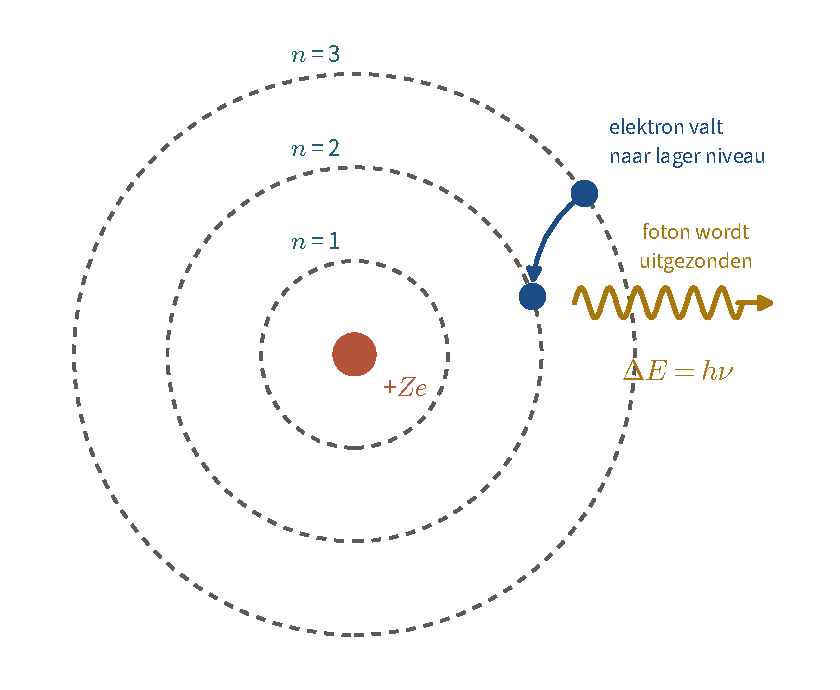
\includegraphics[width=0.5\linewidth]{Figuren/bohr}
    \caption{Schematische voorstelling van het model van Bohr: een elektron valt van baan $n=3$ naar $n=2$ en zendt een foton uit met $h\nu = \Delta E$.}
    \label{fig:bohr-model}
\end{figure}

\paragraph{De grenzen van het model.}
Toch bleek het model van Bohr ontoereikend, om drie fundamentele redenen:
\begin{enumerate}
\item Het werkt enkel voor systemen met precies één elektron (H, He$^+$, Li$^{2+}$). Voor elk atoom met meer elektronen geeft het verkeerde resultaten, omdat het de onderlinge afstoting van de elektronen niet beschrijft.
\item De kwantisatievoorwaarde~\eqref{eq:bohr-kwantisatie} wordt \emph{opgelegd} omdat ze het juiste antwoord geeft. Het model verklaart niet \emph{waarom} enkel die banen zijn toegelaten, en ook niet waarom een elektron op zo'n baan niet straalt.
\item Het beschrijft het elektron als een klassiek deeltje met een precieze plaats en snelheid op een baan. Dat beeld is onverenigbaar met het golfkarakter van materie (\S\ref{sec:materiegolf}).
\end{enumerate}
Een kleine aanpassing van de klassieke mechanica volstaat dus niet. Er was een nieuw kader nodig, waarin kwantisatie niet wordt opgelegd maar vanzelf uit de vergelijkingen volgt. Dat kader bouwen we in de volgende twee secties op.

\subsection{Atomaire spectra}
\label{sec:atomaire-spectra}

Valt een elektron terug naar een lager niveau, dan wordt het energieverschil uitgezonden als een foton met $h\nu = \Delta E$: een \emph{emissiespectrum}. Omgekeerd absorbeert een atoom enkel fotonen waarvan de energie precies overeenkomt met het verschil tussen twee niveaus: een \emph{absorptiespectrum}, met donkere lijnen bij dezelfde golflengten. Voor waterstof vat de formule van Rydberg, die we hierboven uit het model van Bohr afleidden, alle overgangen samen:
\begin{equation}
\boxed{
\frac{1}{\lambda} = R_H\left(\frac{1}{n_i^2}-\frac{1}{n_j^2}\right), \qquad n_j > n_i
}
\end{equation}
met $R_H = \SI{1.097e7}{\per\meter}$. Overgangen naar $n_i=1$ vormen de Lyman-reeks (UV), naar $n_i=2$ de Balmer-reeks (deels zichtbaar) en naar $n_i=3$ de Paschen-reeks (infrarood) (figuur~\ref{fig:waterstofspectrum}).

\begin{figure}[htb]
    \centering
    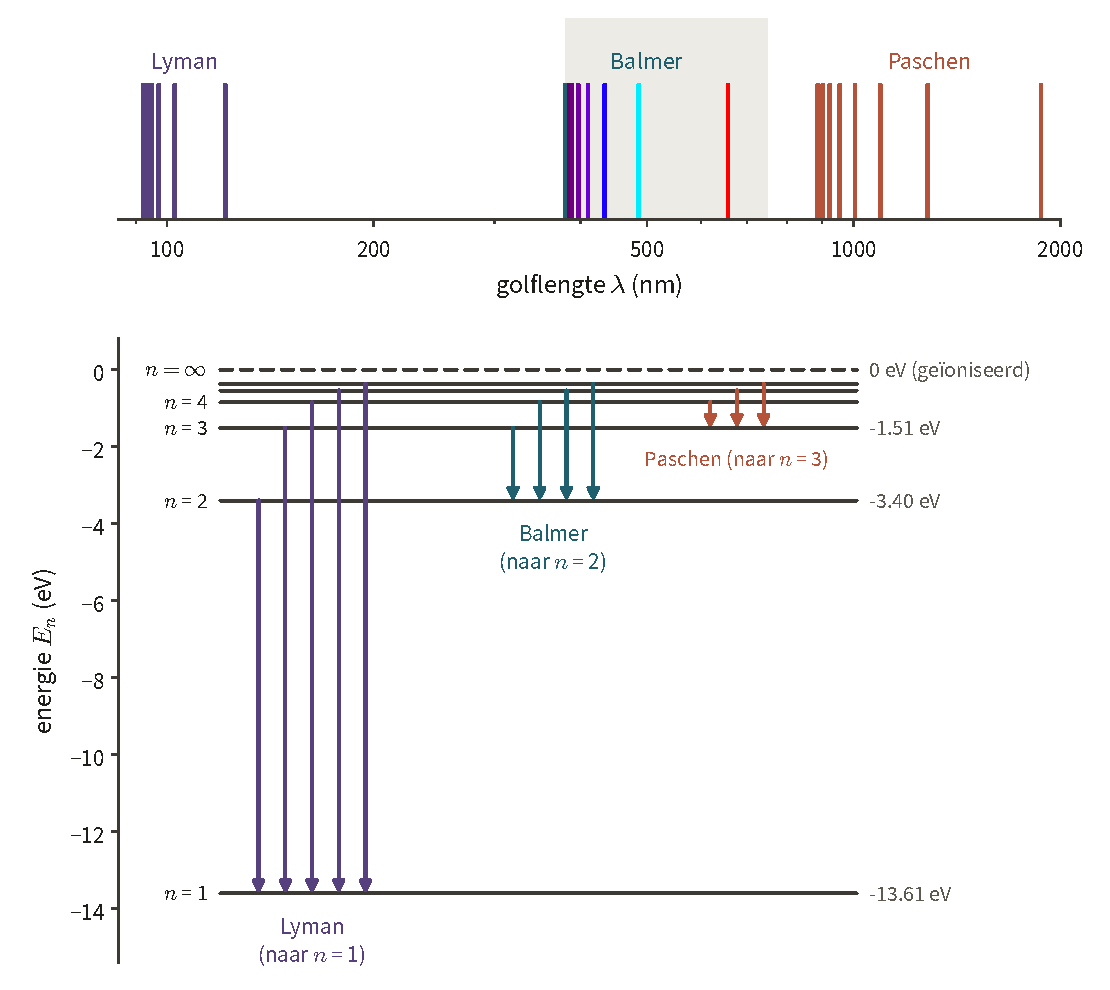
\includegraphics[width=0.62\linewidth]{Figuren/waterstof}
    \caption{Lijnenspectrum van waterstof (boven) en de overgangen tussen energieniveaus die het veroorzaken (onder): Lyman (naar $n=1$), Balmer (naar $n=2$) en Paschen (naar $n=3$).}
    \label{fig:waterstofspectrum}
\end{figure}

\begin{voorbeeld}{Twee lijnen van waterstof}
De overgang $n=2 \to n=1$ geeft $\Delta E = -3.40 - (-13.6) = \SI{10.2}{eV}$, dus
\[
\lambda = \frac{hc}{\Delta E} = \frac{(6.626\times 10^{-34})(2.998\times 10^{8})}{(10.2)(1.602\times 10^{-19})} = \SI{122}{\nano\meter},
\]
de eerste Lyman-lijn in het UV. De rode H$_\alpha$-lijn is de overgang $3 \to 2$:
\[
\frac{1}{\lambda} = (1.097\times10^{7})\left(\frac{1}{4}-\frac{1}{9}\right) = \SI{1.524e6}{\per\meter} \quad\Rightarrow\quad \lambda = \SI{656}{\nano\meter}.
\]
Sterrenkundigen herkennen waterstof in verre sterrenstelsels aan precies deze lijn.
\end{voorbeeld}

Elk element heeft andere energieniveaus en dus een eigen spectrum, een vingerafdruk. Dat zie je in het dagelijks leven: natriumdamp kleurt een vlam en de oude straatlampen geel (\SI{589}{\nano\metre}), neon gloeit rood-oranje, en vuurwerk krijgt zijn kleuren van strontium (rood), barium (groen) en koper (blauw). In het labo bepaalt men zo de samenstelling van een staal: in atoomemissie- en atoomabsorptiespectrometrie meet men de intensiteit van de lijnen van een element om zijn concentratie te bepalen, tot ver onder een milligram per liter.

\begin{casusuitgewerkt}{scherpe lijnen}
Een atoom of molecule kan enkel bepaalde energieën hebben. Het absorbeert dus enkel fotonen waarvan de energie precies overeenkomt met het verschil tussen twee toegelaten niveaus, $h\nu = \Delta E$. Daarom bestaat een spectrum uit scherpe lijnen.

Bij \SI{4.26}{\micro\metre} hoort
\[
\Delta E = \frac{hc}{\lambda} = \frac{(6.626\times10^{-34})(2.998\times10^{8})}{4.26\times10^{-6}} = \SI{4.66e-20}{\joule} = \SI{0.29}{\electronvolt} = \SI{28}{\kilo\joule\per\mole}.
\]
Dat is veel kleiner dan de elektronische overgangen van waterstof, die enkele elektronvolt bedragen (\SI{10.2}{\electronvolt} voor de eerste Lyman-lijn, \SI{1.9}{\electronvolt} voor H$_\alpha$). Bij de lijn van CO$_2$ verandert dus geen elektron van orbitaal. Er moeten nog andere, kleinere energietrappen bestaan: die van de molecule als geheel (\S\ref{sec:moleculaire-beweging}).

\emph{Volgende vraag.} Het model van Bohr legt de kwantisatie op zonder te verklaren waar ze vandaan komt. Waarom zijn de energieniveaus discreet?
\end{casusuitgewerkt}

\section{Materie als golf}
\label{sec:materiegolf}

Het antwoord op die vraag begint met een verrassende vaststelling: niet enkel licht, ook materie gedraagt zich als een golf.

\subsection{Golf of deeltje? Wat de experimenten toonden}

Rond 1920 lag er een verwarrende verzameling waarnemingen op tafel. Sommige experimenten toonden dat licht een golf is, andere dat het uit deeltjes bestaat. Kort daarna bleek hetzelfde te gelden voor elektronen (tabel~\ref{tab:dualiteit}).

\begin{table}[htb]
\centering
\caption{Waarnemingen die het duale karakter van licht en materie aantoonden.}
\label{tab:dualiteit}
\begin{tabular}{p{0.18\linewidth}p{0.36\linewidth}p{0.36\linewidth}}
\toprule
 & gedrag als golf & gedrag als deeltje \\
\midrule
licht & interferentie achter twee spleten (Young, 1801); buiging van röntgenstraling aan kristallen (Von Laue, Bragg, 1912) & foto-elektrisch effect (1905); botsing van röntgenfotonen met elektronen (Compton, 1923) \\
elektronen & buiging aan een nikkelkristal (Davisson en Germer, 1927) en aan dunne metaalfolie (Thomson, 1927) & sporen in een nevelkamer; afzonderlijke inslagen op een scherm \\
\bottomrule
\end{tabular}
\end{table}

\paragraph{Licht als golf.} Dat licht een golf is, leek sinds 1801 bewezen. Thomas Young liet licht door twee smalle spleten vallen en zag op een scherm een patroon van heldere en donkere banden. Waar de golven uit beide spleten in fase aankomen, versterken ze elkaar; waar een top een dal ontmoet, doven ze elkaar uit. Dat heet \emph{interferentie}, en enkel golven doen dat. Ook röntgenstraling buigt af aan de regelmatige rijen atomen in een kristal, wat de basis is van de röntgendiffractie waarmee men vandaag kristalstructuren bepaalt.

\paragraph{Licht als deeltje.} Het foto-elektrisch effect toonde dat licht zijn energie in pakketjes $h\nu$ afgeeft. In 1923 ging Arthur Compton een stap verder. Hij stuurde röntgenstraling op grafiet en zag dat de verstrooide straling een iets langere golflengte had, afhankelijk van de hoek. Dat kon hij enkel verklaren als een botsing tussen twee biljartballen: een foton botst op een elektron en geeft het een deel van zijn energie en zijn \emph{impuls} mee. Een foton heeft dus een impuls. Voor een deeltje zonder massa dat met de lichtsnelheid beweegt, is $E = pc$, en met $E = hc/\lambda$ volgt
\[
p = \frac{h}{\lambda}.
\]

\subsection{Het golfkarakter van materie}

\paragraph{De hypothese van De Broglie.}
In 1924, in zijn doctoraat, keerde Louis de Broglie die redenering om. Als licht, dat we als golf kenden, ook deeltjeseigenschappen heeft, dan heeft materie, die we als deeltjes kennen, misschien ook golfeigenschappen. Aan elk deeltje met impuls $p=mv$ kende hij dezelfde relatie toe als aan een foton:
\begin{equation}
\boxed{
\lambda=\frac{h}{p}=\frac{h}{mv}
}
\end{equation}
Dit betekent niet dat een elektron letterlijk als een klein, golvend draadje door de ruimte beweegt. Het betekent dat het gedrag van een deeltje beschreven wordt door een golf, en dat het onder geschikte omstandigheden interferentie en buiging vertoont. Voor macroscopische voorwerpen is de impuls zo groot dat de golflengte onmeetbaar klein is. Voor elektronen kan ze vergelijkbaar zijn met de afstand tussen atomen.

\begin{voorbeeld}{De De Broglie-golflengte van een elektron en een wandelende persoon}
Een elektron dat vanuit rust over een spanning $U$ wordt versneld, krijgt een kinetische energie $eU = \tfrac12 m_e v^2 = p^2/2m_e$. Zijn impuls is dus $p = \sqrt{2m_e eU}$, en zijn golflengte
\[
\lambda = \frac{h}{\sqrt{2m_e eU}} .
\]
Voor $U = \SI{150}{\volt}$:
\[
\lambda = \frac{6.626\times10^{-34}}{\sqrt{2(9.109\times10^{-31})(1.602\times10^{-19})(150)}} = \SI{1.00e-10}{\metre} = \SI{0.100}{\nano\metre},
\]
precies de afstand tussen atomen in een kristal. Zo'n elektronen buigen dus af aan een kristal, en de elektronenmicroscoop maakt hier gebruik van.

Een wandelaar ($m = \SI{75}{\kilo\gram}$, $v = \SI{1.5}{\metre\per\second}$) heeft $p = \SI{112.5}{\kilo\gram\metre\per\second}$ en
\[
\lambda = \frac{6.626\times10^{-34}}{112.5} = \SI{5.9e-36}{\metre},
\]
ontelbare grootteordes kleiner dan een atoomkern. Het golfkarakter van een mens is daarom volledig onwaarneembaar. De relatie van De Broglie geldt voor alle materie, maar ze wordt enkel merkbaar bij zeer lichte deeltjes.
\end{voorbeeld}

\paragraph{De bevestiging: elektronen buigen af.}
Drie jaar later werd de hypothese bevestigd, deels bij toeval. Clinton Davisson en Lester Germer schoten bij Bell Labs elektronen van \SI{54}{\electronvolt} loodrecht op een nikkelkristal en maten hoeveel elektronen onder elke hoek terugkaatsten (figuur~\ref{fig:davisson-germer}). Ze vonden een scherpe piek bij \SI{50}{\degree}, precies wat je verwacht voor een golf die buigt aan de rijen nikkelatomen. Een golf weerkaatst op die rijen, met onderlinge afstand $d = \SI{0.215}{\nano\metre}$, versterkt in de richting $\varphi$ waarvoor het wegverschil een hele golflengte is: $d\sin\varphi = \lambda$. Met de formule van De Broglie is
\[
\lambda = \frac{h}{\sqrt{2m_e eU}} = \SI{0.167}{\nano\metre}
\quad\Longrightarrow\quad
\sin\varphi = \frac{0.167}{0.215} = 0.776, \quad \varphi = \SI{51}{\degree}.
\]
Vrijwel tegelijk stuurde George Thomson elektronen door een dunne goudfolie en zag hij ringen zoals bij röntgenstraling. Sindsdien is interferentie aangetoond met neutronen, heliumatomen en zelfs met voetbalvormige C$_{60}$-moleculen van 60 koolstofatomen.

\begin{figure}[htb]
    \centering
    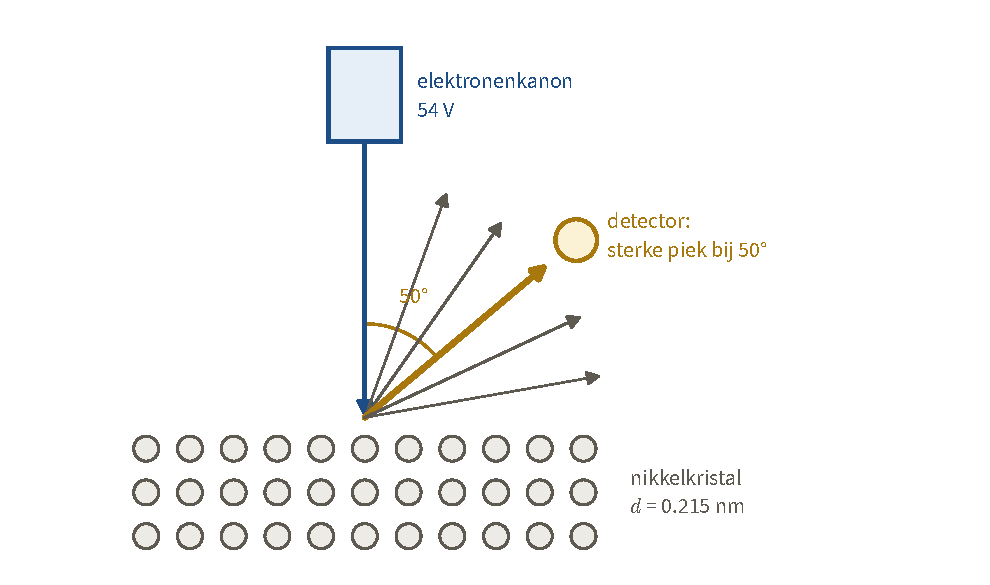
\includegraphics[width=0.62\linewidth]{Figuren/davisson_germer}
    \caption{Het experiment van Davisson en Germer (1927). Elektronen van \SI{54}{\electronvolt} worden door een nikkelkristal sterk teruggekaatst onder een hoek van \SI{50}{\degree}: ze buigen af als golven met de golflengte van De Broglie.}
    \label{fig:davisson-germer}
\end{figure}

\subsection{De dubbelspleetproef}
\label{sec:dubbelspleet}

De meest overtuigende proef is de dubbelspleetproef van Young, maar dan met elektronen. Stuur je een elektronenbundel door twee fijne spleten, dan ontstaat op een scherm een interferentiepatroon van heldere en donkere banden, zoals bij licht. Dat patroon is enkel te verklaren als elk elektron zich als een golf door \emph{beide} spleten tegelijk beweegt: de twee deelgolven versterken of doven elkaar op het scherm.

Het wordt nog vreemder wanneer de bron zo zwak is dat er telkens maar één elektron onderweg is. Dan verschijnt op het scherm telkens één scherp punt: het elektron wordt als deeltje gedetecteerd, op één plaats. Waar het volgende elektron aankomt, is niet te voorspellen. Pas na duizenden elektronen ontstaat het patroon van banden (figuur~\ref{fig:dubbelespleet}). Elk afzonderlijk elektron gedraagt zich dus bij de detectie als een deeltje, maar de verdeling van vele inslagen is die van een golf. Probeer je te meten door welke spleet een elektron gaat, dan verdwijnt het patroon. Licht en materie zijn dus geen golf óf deeltje; ze vertonen beide aspecten, afhankelijk van wat je meet.

\begin{figure}[htb]
    \centering
    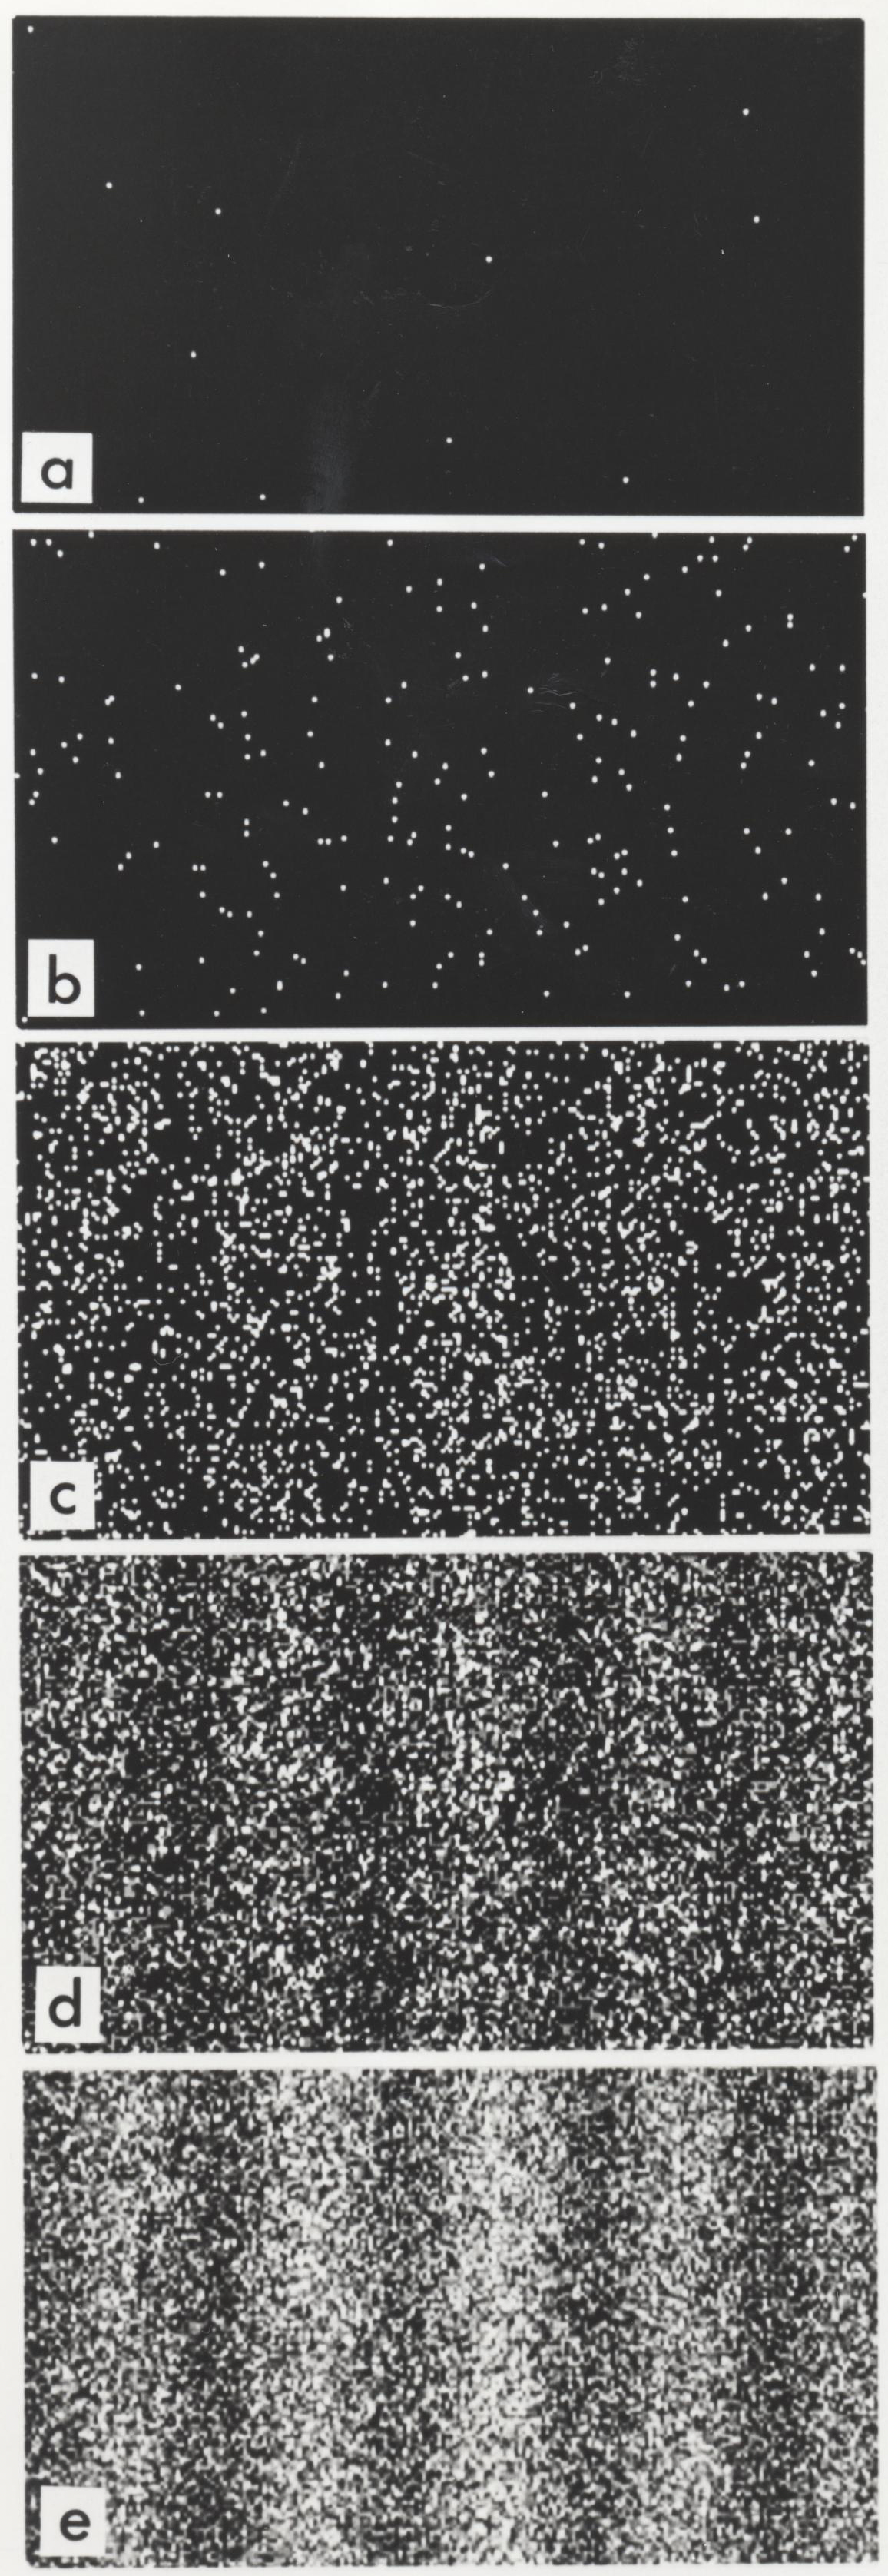
\includegraphics[width=0.3\linewidth]{Afbeeldingen/Double-slit_experiment_results_Tonomura_2.jpg}
    \caption{Dubbelspleetexperiment met afzonderlijke elektronen: na 11 (a), 200 (b), 6000 (c), 40\,000 (d) en 140\,000 (e) elektronen.}
    \label{fig:dubbelespleet}
\end{figure}

\begin{toepassing}{Een Brussels weetje: de Solvayconferentie van 1927}
Ernest Solvay, rijk geworden met zijn sodaproces (\ce{Na2CO3}, nog steeds de basis van de glasindustrie), financierde vanaf 1911 de Solvayconferenties voor natuurkunde in Brussel. De vijfde, in oktober 1927, ging over ``elektronen en fotonen''. Op de groepsfoto staan onder meer Einstein, Bohr, Planck, Marie Curie, Schr\"odinger, Heisenberg, De Broglie, Dirac en Pauli: 17 van de 29 deelnemers hadden of kregen een Nobelprijs. Er werd hevig gediscussieerd over de betekenis van de golffunctie, het onderwerp van de volgende sectie. Einsteins ``God dobbelt niet'' en Bohrs antwoord ``Einstein, vertel God niet wat Hij moet doen'' stammen uit die discussies.
\end{toepassing}

\section{De golffunctie en de Schr\"odingervergelijking}

\subsection{De golffunctie en haar betekenis}
\label{sec:golffunctie}

\paragraph{Wat beschrijft een golf?}
Elke golf wordt beschreven door een functie die op elke plaats en elk tijdstip de \emph{amplitude} geeft: de uitwijking van een gitaarsnaar $y(x,t)$, de luchtdruk bij geluid, of bij licht de elektrische veldsterkte. Die amplitude kan positief of negatief zijn: een snaar wijkt naar boven of naar onder uit. Wat je waarneemt, is echter niet de amplitude zelf, maar de \emph{intensiteit}, de energie die per seconde aankomt. Die is evenredig met het \emph{kwadraat} van de amplitude. Een lichtmeter of je oog meet dus amplitude in het kwadraat.

Denk nu aan fotonen. Laat je heel zwak licht op een fotoplaat vallen, dan komen de fotonen één voor één aan, elk op één punt. Waar de amplitude groot is, komen er veel aan; waar ze nul is, geen. Het kwadraat van de amplitude zegt dus \emph{hoe waarschijnlijk} het is dat een foton op een bepaalde plaats aankomt.

\paragraph{De golffunctie van een elektron.}
In de kwantummechanica wordt de toestand van een elektron, of van elk ander deeltje, beschreven door een \emph{golffunctie} $\psi(\vec r, t)$: de amplitude van de materiegolf op elke plaats $\vec r$ en elk tijdstip $t$. De golffunctie bevat alle informatie die over het deeltje te kennen is. Ze is zelf geen meetbare grootheid; je kunt nergens ``$\psi$ aflezen''. Ze kan positief of negatief zijn, en in het algemeen is ze zelfs een \emph{complex} getal.

Waarom complex? Een golf heeft op elke plaats twee kenmerken: hoe groot de uitwijking is (de amplitude) en waar in de trilling ze zit (de \emph{fase}: op een top, in een dal, of ertussen). Een complex getal $\psi = |\psi|\,e^{i\phi}$ draagt die twee in één getal. Voor een elektron dat met welbepaalde impuls $p = \hbar k$ in de $x$-richting beweegt, is de golffunctie $\psi = A\,e^{i(kx-\omega t)}$. Het reële en het imaginaire deel zijn dan een cosinus- en een sinusgolf die een kwart golflengte verschoven zijn (figuur~\ref{fig:golffunctie}a).

\paragraph{De betekenis van $\psi^*\psi$.}
Max Born gaf in 1926 de interpretatie, naar analogie met de fotonen: het kwadraat van de amplitude is een kans. Omdat $\psi$ complex kan zijn, neem je niet gewoon $\psi^2$, maar het product van $\psi$ met zijn \emph{complex toegevoegde} $\psi^*$. Schrijf je $\psi = a + ib$, dan is $\psi^* = a - ib$ en
\[
\psi^*\psi = (a-ib)(a+ib) = a^2 + b^2 = |\psi|^2 .
\]
Dat is altijd een reëel, positief getal, zoals een kans moet zijn. Het wordt de \emph{waarschijnlijkheidsdichtheid} genoemd: de kans per volume-eenheid om het deeltje op die plaats aan te treffen (eenheid \si{\per\metre\cubed}). De kans om het deeltje op tijdstip $t$ in een klein volume $\dd V$ rond $\vec r$ te vinden, is
\begin{equation}
\boxed{
\dd P = \psi^*(\vec{r},t)\,\psi(\vec{r},t)\,\dd V = |\psi(\vec{r},t)|^2\,\dd V .
}
\end{equation}
De kans om het in een groter gebied $\Omega$ te vinden, is de integraal over dat gebied, het oppervlak onder de kromme in figuur~\ref{fig:golffunctie}b:
\[
P_\Omega = \int_\Omega |\psi|^2\,\dd V .
\]
Omdat het deeltje zich ergens moet bevinden, is de totale kans gelijk aan één:
\begin{equation}
\int_{\text{volledige ruimte}} |\psi|^2\,\dd V = 1 .
\label{eq:normering}
\end{equation}
Een golffunctie die hieraan voldoet, heet \emph{genormeerd}.

\begin{figure}[htb]
    \centering
    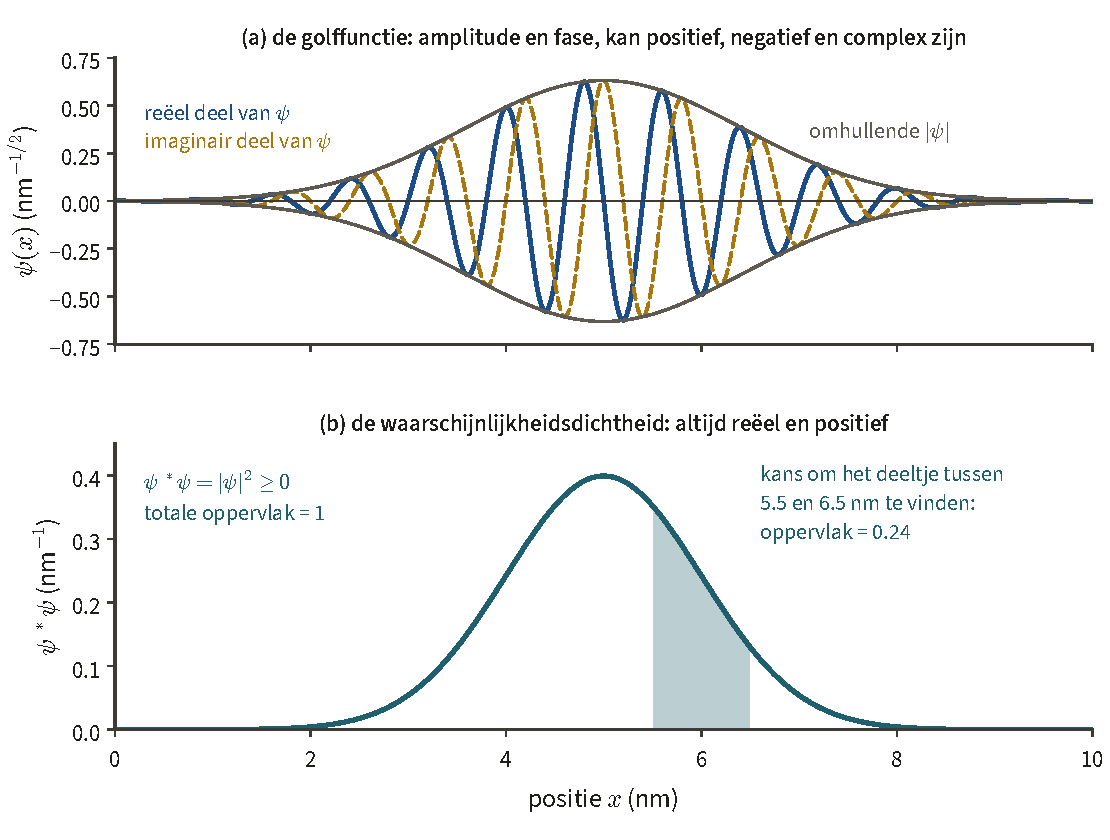
\includegraphics[width=0.8\linewidth]{Figuren/golffunctie_betekenis}
    \caption{(a) De golffunctie van een elektron dat in een beperkt gebied naar rechts beweegt. Het reële en het imaginaire deel trillen een kwart golflengte verschoven; de omhullende $|\psi|$ geeft de grootte. (b) De waarschijnlijkheidsdichtheid $\psi^*\psi$. De fase valt weg, en wat overblijft is altijd positief. Het gearceerde oppervlak is de kans om het elektron tussen \SI{5.5}{} en \SI{6.5}{\nano\metre} aan te treffen.}
    \label{fig:golffunctie}
\end{figure}

Voor de golf $\psi = A\,e^{i(kx-\omega t)}$ van een elektron met welbepaalde impuls is $\psi^*\psi = A\,e^{-i(kx-\omega t)}\,A\,e^{i(kx-\omega t)} = A^2$: overal even groot. Een elektron waarvan de impuls exact gekend is, kan overal zijn. Wil je het lokaliseren, zoals in figuur~\ref{fig:golffunctie}, dan moet je golven met verschillende impulsen combineren. Plaats en impuls zijn dus nooit tegelijk exact bepaald; dat is de \emph{onzekerheidsrelatie} van Heisenberg.

\paragraph{Waarom de fase er toch toe doet.}
In $\psi^*\psi$ valt de fase weg. Toch is ze belangrijk zodra twee golven samenkomen. In de dubbelspleetproef is de golffunctie op het scherm de som $\psi = \psi_1 + \psi_2$ van de golven uit elke spleet, en de kans is $|\psi_1 + \psi_2|^2$, niet $|\psi_1|^2 + |\psi_2|^2$. Waar beide in fase aankomen, versterken ze elkaar; waar ze tegengesteld zijn, wordt de kans nul. Dat is de oorsprong van de donkere banden. Hetzelfde mechanisme vormt verderop de chemische binding: twee atoomorbitalen die in fase overlappen, vergroten de kans om het elektron tussen de kernen te vinden (\S\ref{sec:molecuulorbitalen}).

De kwantummechanica voorspelt dus niet waar één elektron zal worden aangetroffen, wel hoe vaak elke plaats voorkomt als je de meting vele keren herhaalt. Dat is precies wat de dubbelspleetproef toont: elke inslag is willekeurig, maar de verdeling volgt $|\psi|^2$. Het is ook de eerste keer in deze cursus dat waarschijnlijkheid een fundamentele rol speelt, in plaats van onze onwetendheid te weerspiegelen. In hoofdstuk~\ref{ch:spontaniteit} ligt diezelfde idee, een groot aantal mogelijke toestanden met elk een waarschijnlijkheid, aan de basis van de entropie.

\subsection{De Schr\"odingervergelijking}

\paragraph{Waar komt de vergelijking vandaan?}
De golffunctie zegt wat we kunnen weten, maar welke golffuncties zijn mogelijk voor een elektron in een atoom of een molecule? Erwin Schr\"odinger stelde daarvoor in 1926 een vergelijking op. Ze kan niet worden afgeleid uit de klassieke fysica, maar je kunt wel zien waarom ze deze vorm heeft.

Neem een vrij deeltje met impuls $p$. Volgens De Broglie hoort daar een golf bij met golflengte $\lambda = h/p$, bijvoorbeeld $\psi = A\sin(kx)$ met golfgetal $k = 2\pi/\lambda = p/\hbar$. Leid je die golf twee keer af, dan krijg je
\[
\frac{\dd^2\psi}{\dd x^2} = -k^2\psi = -\frac{p^2}{\hbar^2}\,\psi .
\]
Vermenigvuldig met $-\hbar^2/2m$ en gebruik dat de kinetische energie $p^2/2m$ is:
\[
-\frac{\hbar^2}{2m}\frac{\dd^2\psi}{\dd x^2} = \frac{p^2}{2m}\,\psi = E_\mathrm{kin}\,\psi .
\]
Is er ook een potentiële energie $V$, dan is $E_\mathrm{kin} = E - V$, met $E$ de totale energie. Schr\"odinger postuleerde dat deze relatie ook geldt wanneer $V$ van plaats tot plaats verandert. Zo krijg je, voor één deeltje in één dimensie en een toestand met welbepaalde energie, de \emph{tijdsonafhankelijke Schr\"odingervergelijking}:
\begin{equation}
\boxed{
-\frac{\hbar^2}{2m}\frac{\partial^2\psi}{\partial x^2} + V(x)\psi = E\psi,
}
\label{eq:Schrodinger}
\end{equation}
met $\hbar=h/2\pi$, $m$ de massa van het deeltje, $V(x)$ de potentiële energie en $E$ de totale energie.

\paragraph{Wat de vergelijking zegt.}
De eerste term is de kinetische energie, en die hangt af van de \emph{kromming} van $\psi$. Waar $E - V$ groot is, beweegt het deeltje snel: de golf is daar sterk gekromd, met een korte golflengte. Waar $E - V$ klein is, is de golf vlakker. En waar $V > E$, een gebied dat klassiek verboden is, kromt de golf de andere kant op: ze trilt niet meer, maar sterft exponentieel uit. Het deeltje dringt dus een klein stukje door in een gebied waar het klassiek niet mag komen. Is zo'n gebied dun genoeg, dan kan het er zelfs doorheen: het \emph{tunneleffect}, waarop de rastertunnelmicroscoop en het geheugen in een usb-stick berusten.

De Schr\"odingervergelijking speelt dezelfde rol als de wetten van Newton in de klassieke mechanica. Ze levert echter geen baan of exacte positie, maar de golffuncties die voor het systeem mogelijk zijn, en de bijbehorende energieën.

\paragraph{Welke oplossingen zijn toegelaten?}
Niet elke wiskundige oplossing van~\eqref{eq:Schrodinger} beschrijft een fysische toestand. Een aanvaardbare golffunctie moet aan drie voorwaarden voldoen:
\begin{itemize}
\item \textbf{Eindig}: $\psi$ mag nergens oneindig worden, want dan zou $|\psi|^2$ een oneindige kans per volume geven op die plaats, wat fysisch onmogelijk is.
\item \textbf{Continu}: $\psi$ mag geen sprongen maken, en bij een eindige potentiaal ook haar eerste afgeleide niet. De vergelijking bevat een tweede afgeleide, en die bestaat enkel als $\psi$ vloeiend verloopt.
\item \textbf{Normeerbaar}: de totale kans~\eqref{eq:normering} moet gelijk aan één kunnen worden gemaakt. Voor een gebonden deeltje moet $\psi$ daarom naar nul gaan op grote afstand.
\end{itemize}
Juist deze voorwaarden laten voor een opgesloten deeltje slechts bepaalde golffuncties toe, en dus slechts bepaalde energieën. De kwantisatie is geen extra postulaat meer zoals bij Bohr; ze volgt uit de vergelijking zelf. Dat maken we in de volgende paragraaf concreet.

Voor een elektron in een atoom is $V$ de Coulombaantrekking door de kern. De oplossingen zijn de atoomorbitalen en hun energieniveaus (\S\ref{sec:waterstofatoom}). Verderop passen we dezelfde vergelijking toe op heel andere potentialen: een molecule die vrij beweegt in een vat, die roteert of die trilt (\S\ref{sec:moleculaire-beweging}). Telkens volgen er vanzelf discrete energieniveaus en nieuwe kwantumgetallen uit.

Ook de stabiliteit van het atoom volgt nu. Een toestand met welbepaalde energie heeft een kansverdeling $|\psi|^2$ die niet verandert in de tijd: er beweegt geen lading heen en weer, en er wordt dus niets uitgestraald. De laagste toegelaten oplossing is de grondtoestand. Een toestand waarin het elektron in de kern stort, is geen aanvaardbare oplossing: hij zou een oneindig sterk gekromde golffunctie vereisen, met een oneindige kinetische energie.

\subsection{Discrete energieniveaus}
\label{sec:discrete-energieniveaus}

Een gitaarsnaar die aan beide uiteinden vastzit, kan enkel trillen in patronen met een geheel aantal halve golflengten, net zoals het stralingsveld in de holte van figuur~\ref{fig:trillingsmodi}. Voor een materiegolf die opgesloten zit, geldt hetzelfde. Dat maken we concreet met het eenvoudigste voorbeeld: een deeltje met massa $m$ dat vrij beweegt in een ééndimensionale \emph{doos} met lengte $L$, en de wanden niet kan verlaten ($V=0$ binnen, $V=\infty$ buiten).

\emph{Stap 1: de vergelijking.} Binnen de doos is $V=0$ en wordt~\eqref{eq:Schrodinger}
\[
-\frac{\hbar^2}{2m}\frac{\dd^2\psi}{\dd x^2} = E\psi
\qquad\text{of}\qquad
\frac{\dd^2\psi}{\dd x^2} = -k^2\psi, \quad k=\frac{\sqrt{2mE}}{\hbar}.
\]
Welke functie geeft na twee keer afleiden zichzelf terug, met een minteken? Een sinus en een cosinus. De algemene oplossing is dus $\psi(x)=A\sin(kx)+B\cos(kx)$.

\emph{Stap 2: de randvoorwaarden.} Buiten de doos is $\psi = 0$, want het deeltje kan er niet zijn. Omdat $\psi$ continu moet zijn, moet ze ook aan de wanden nul zijn: $\psi(0)=0$ en $\psi(L)=0$. De eerste voorwaarde geeft $B=0$, want $\cos 0 = 1$. De tweede geeft $A\sin(kL)=0$. Met $A=0$ zou er geen deeltje zijn, dus moet $\sin(kL)=0$:
\[
kL = n\pi, \qquad n=1,2,3,\ldots
\]
Er passen dus een geheel aantal halve golflengten in de doos, $L = n\lambda/2$, net als bij de snaar.

\emph{Stap 3: de energie.} Met $k = n\pi/L$ in $E=\hbar^2k^2/(2m)$ volgt
\begin{equation}
\boxed{
E_n = \frac{n^2h^2}{8mL^2}, \qquad n=1,2,3,\ldots
}
\label{eq:deeltje-in-doos}
\end{equation}

\emph{Stap 4: de normering.} De constante $A$ volgt uit~\eqref{eq:normering}: $\int_0^L A^2\sin^2(n\pi x/L)\,\dd x = A^2 L/2 = 1$, dus $A = \sqrt{2/L}$ en
\[
\psi_n(x) = \sqrt{\frac{2}{L}}\,\sin\frac{n\pi x}{L}.
\]

De kwantisatie volgt hier uitsluitend uit de randvoorwaarden; er is geen extra postulaat nodig zoals bij Bohr. Figuur~\ref{fig:deeltje-doos} toont de eerste vier oplossingen. Drie eigenschappen komen in elk kwantumsysteem terug:
\begin{itemize}
\item De laagste energie is \emph{niet nul}: $E_1 = h^2/(8mL^2)$. Een opgesloten deeltje kan nooit volledig stilliggen. Deze \emph{nulpuntsenergie} vinden we terug bij de trillende molecule (\S\ref{sec:vibratie}).
\item Hogere toestanden hebben meer \emph{knopen}, punten waar $\psi = 0$: toestand $n$ heeft er $n-1$. Meer knopen betekent een sterker gekromde golf, dus een hogere kinetische energie.
\item De niveaus liggen verder uit elkaar naarmate de doos kleiner of het deeltje lichter is ($E_n \propto 1/mL^2$). Daarom is kwantisatie belangrijk voor elektronen in atomen en verwaarloosbaar voor een knikker in een doos.
\end{itemize}

\begin{figure}[htb]
    \centering
    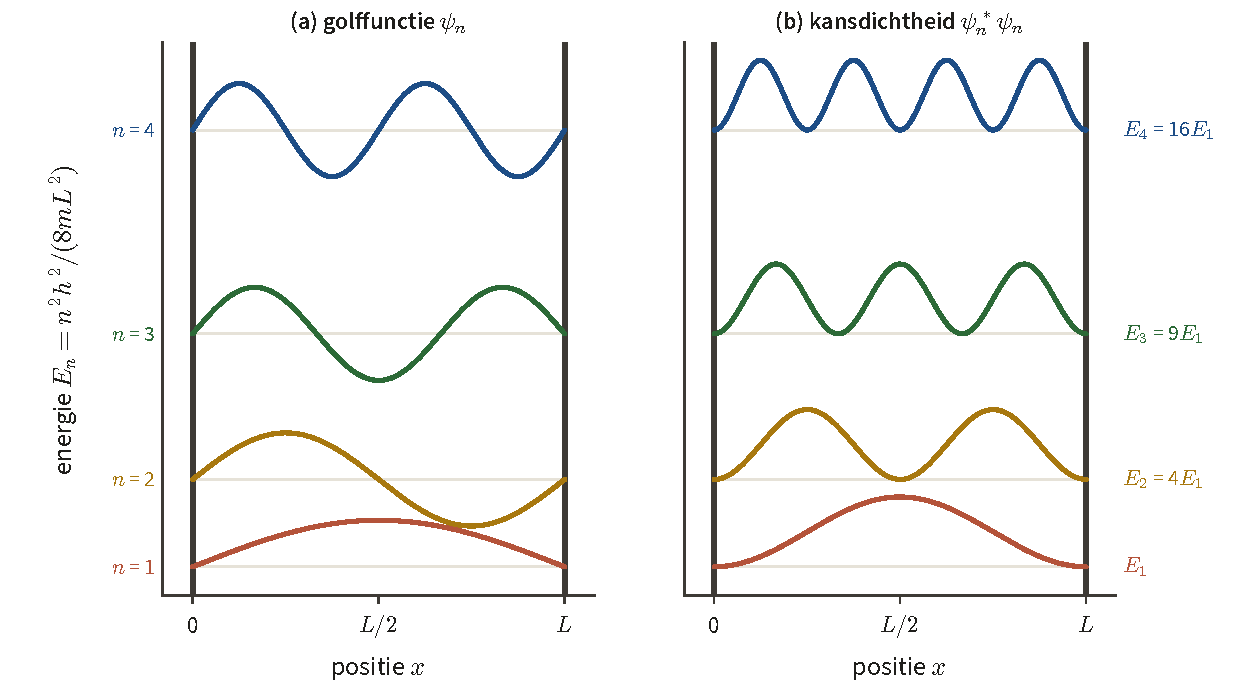
\includegraphics[width=0.85\linewidth]{Figuren/deeltje_doos}
    \caption{Deeltje in een doos. (a) De golffuncties van de eerste vier toestanden, elk getekend op de hoogte van zijn energie $E_n = n^2E_1$. (b) De waarschijnlijkheidsdichtheden $\psi_n^*\psi_n$. In toestand $n=2$ is de kans om het deeltje in het midden te vinden nul.}
    \label{fig:deeltje-doos}
\end{figure}

\begin{voorbeeld}{Waar zit het deeltje, en hoe groot zijn de energiesprongen?}
\emph{Kans in het middelste derde.} In de grondtoestand is de kans om het deeltje tussen $L/3$ en $2L/3$ te vinden
\[
P = \int_{L/3}^{2L/3}\frac{2}{L}\sin^2\frac{\pi x}{L}\,\dd x = \frac13 + \frac{\sqrt3}{2\pi} = 0.61 .
\]
Een klassiek deeltje dat heen en weer botst, zou even vaak op elke plaats zijn, met een kans van $1/3$. Het kwantumdeeltje in de grondtoestand zit liever in het midden. In toestand $n=2$ is de kans in het exacte midden nul, hoewel het deeltje links en rechts ervan wel kan zijn.

\emph{Een elektron in een doos van \SI{1}{\nano\metre}.} Dat is ongeveer de lengte van een molecule met een rij geconjugeerde dubbele bindingen. Dan is
\[
E_1 = \frac{(6.626\times10^{-34})^2}{8(9.109\times10^{-31})(1.0\times10^{-9})^2} = \SI{6.0e-20}{\joule} = \SI{0.38}{\electronvolt},
\]
en de sprong van $n=1$ naar $n=2$ is $3E_1 = \SI{1.1}{\electronvolt}$, een foton van \SI{1.1}{\micro\metre}. Hoe kleiner de doos, hoe groter de sprong en hoe blauwer het licht. Dat is het principe van \emph{quantum dots}: halfgeleiderkristalletjes van enkele nanometer waarvan de kleur enkel door hun grootte wordt bepaald, gebruikt in de beeldschermen van QLED-televisies.
\end{voorbeeld}

We gebruiken dit resultaat verderop voor de translatie van een molecule in een vat (\S\ref{sec:translatie}).

\subsection{Het waterstofatoom: energieniveaus en orbitalen}
\label{sec:waterstofatoom}

\paragraph{Energieniveaus.}
Voor het waterstofatoom is $V(r)= -e^2/(4\pi\varepsilon_0 r)$, de Coulombaantrekking tussen kern en elektron, nu in drie dimensies. De Schr\"odingervergelijking kan voor deze potentiaal exact worden opgelost. De wiskunde laten we achterwege, maar het resultaat is opvallend: de energieniveaus hangen enkel af van een geheel getal $n$, het hoofdkwantumgetal,
\begin{equation}
E_n = -\frac{\SI{13.6}{eV}}{n^2}, \qquad n = 1,2,3,\ldots
\end{equation}
Het minteken betekent dat het elektron gebonden is. De grondtoestand heeft $E_1 = \SI{-13.6}{eV}$, dan volgen $E_2 = \SI{-3.40}{eV}$ en $E_3 = \SI{-1.51}{eV}$; voor grote $n$ nadert de energie nul. Dat zijn precies de niveaus van Bohr~\eqref{eq:bohr-energie}, maar nu volgt de kwantisatie uit de voorwaarden op de golffunctie, zoals bij het deeltje in een doos. Het model van Bohr was dus een gelukkige gok. De Schr\"odingervergelijking verklaart daarnaast ook atomen met meer elektronen en moleculen, waar Bohr faalde.

\paragraph{Van golffunctie naar orbitaal.}
De oplossingen van de Schr\"odingervergelijking voor een elektron in een atoom heten \emph{atoomorbitalen}. Een orbitaal is dus een toegelaten golffunctie, geen baan. Het elektron draait niet zoals bij Bohr op een cirkel rond de kern; het orbitaal geeft via $|\psi|^2$ aan waar de kans groot of klein is om het elektron aan te treffen. Teken je die kans in drie dimensies, dan krijg je een \emph{elektronenwolk}. Die wolk is geen materiële wolk waarin de lading letterlijk uitgesmeerd is: bij elke meting vind je het elektron op één plaats, maar over vele metingen vormen de plaatsen deze wolk.

Het eenvoudigste orbitaal is de grondtoestand van waterstof, het \emph{1s-orbitaal}:
\[
\psi_{1s}(r) = \frac{1}{\sqrt{\pi a_0^3}}\,e^{-r/a_0},
\]
met $a_0 = \SI{52.9}{\pico\metre}$, opnieuw de straal van Bohr. Het hangt enkel af van de afstand $r$ tot de kern, niet van de richting: het orbitaal is bolvormig. De kans per volume $|\psi_{1s}|^2$ is het grootst in de kern zelf en daalt exponentieel naar buiten (figuur~\ref{fig:radiale-1s}). Betekent dit dat het elektron het vaakst in de kern zit? Nee. Op afstand $r$ ligt een bolschil met dikte $\dd r$ en volume $4\pi r^2\,\dd r$. Hoe verder van de kern, hoe groter die schil. De kans om het elektron op een afstand tussen $r$ en $r+\dd r$ te vinden, is daarom
\[
P(r)\,\dd r = 4\pi r^2\,|\psi_{1s}|^2\,\dd r = \frac{4r^2}{a_0^3}\,e^{-2r/a_0}\,\dd r .
\]
Dicht bij de kern is de schil zeer klein, ver weg is $|\psi|^2$ zeer klein; ertussen ligt een maximum. Stel je de afgeleide van $r^2e^{-2r/a_0}$ gelijk aan nul, dan vind je $2r - 2r^2/a_0 = 0$, dus $r = a_0$. De meest waarschijnlijke afstand tussen het elektron en de kern is exact de straal van Bohr. Het oude model had dus een kern van waarheid: de baan van Bohr is de plaats waar de elektronenwolk het dichtst is.

\begin{figure}[htb]
    \centering
    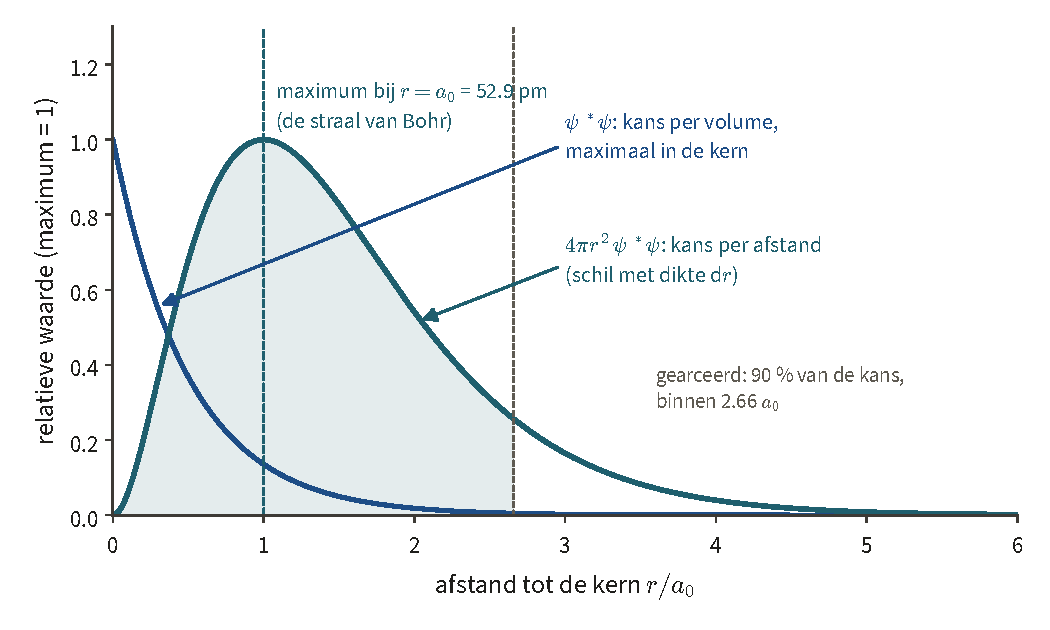
\includegraphics[width=0.7\linewidth]{Figuren/radiale_1s}
    \caption{Het 1s-orbitaal van waterstof. De kans per volume $\psi^*\psi$ is maximaal in de kern, maar de kans per afstand $4\pi r^2\psi^*\psi$ is maximaal bij $r = a_0$, de straal van Bohr. Binnen $2.66\,a_0$ ligt \SI{90}{\percent} van de kans.}
    \label{fig:radiale-1s}
\end{figure}

Een wolk heeft geen scherpe rand. Om toch een vorm te tekenen, kiest men het oppervlak dat bijvoorbeeld \SI{90}{\percent} van de kans omsluit; voor het 1s-orbitaal is dat een bol met straal $2.66\,a_0 = \SI{141}{\pico\metre}$. Voor hogere energieniveaus heeft de Schr\"odingervergelijking ook oplossingen die van de richting afhangen. Zo ontstaan de halter-vormige $p$-orbitalen en de klavervormige $d$-orbitalen (figuur~\ref{fig:orbitalen}). Welke orbitalen bij elk niveau horen, wordt bepaald door drie kwantumgetallen, het onderwerp van de volgende sectie.

\begin{figure}[htb]
    \centering
    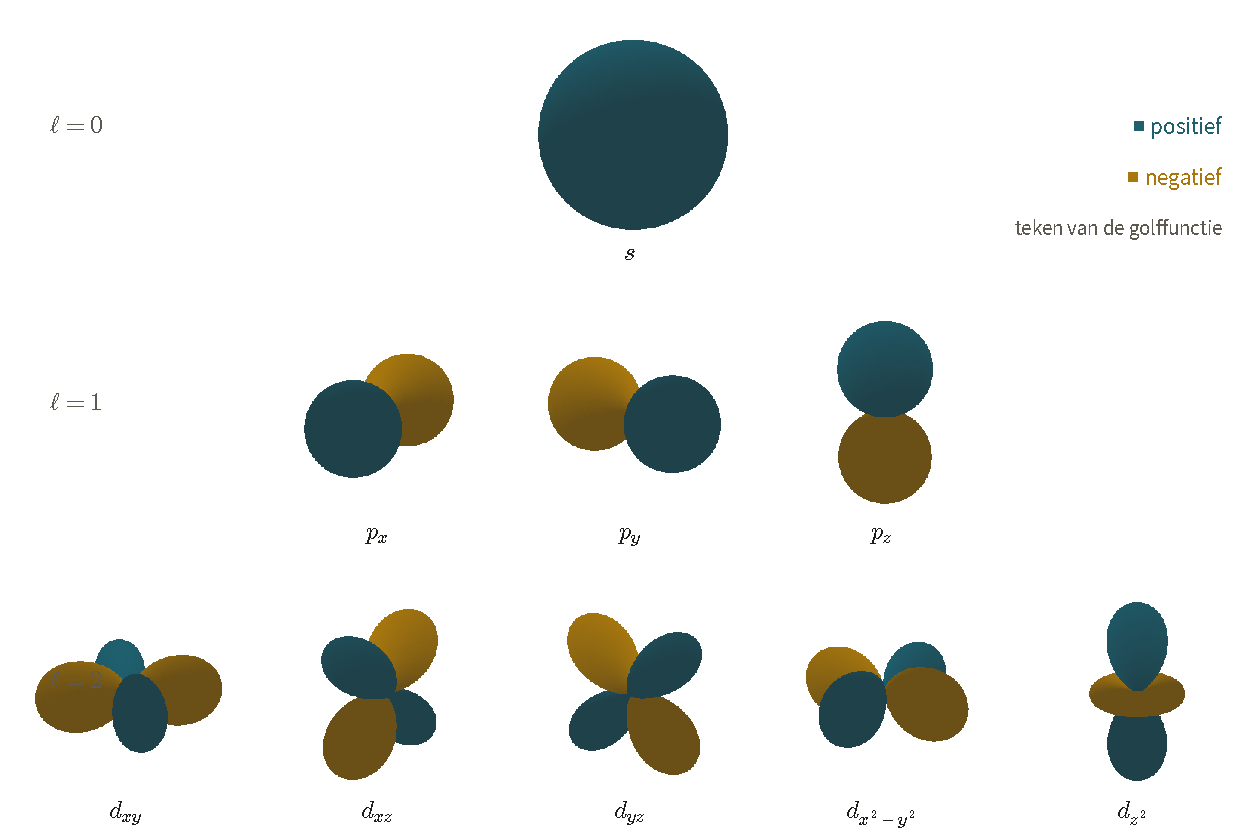
\includegraphics[width=0.62\linewidth]{Figuren/orbitalen}
    \caption{Typische waarschijnlijkheidsverdelingen van $s$-, $p$- en $d$-orbitalen.}
    \label{fig:orbitalen}
\end{figure}

Moleculen hebben naast elektronische ook gekwantiseerde rotatie- en vibratieniveaus (\S\ref{sec:moleculaire-beweging}). Daarom heeft elke stof een eigen ``vingerafdruk''-spectrum, de basis van de spectroscopie in kwaliteitscontrole en procesanalyse.

\section{Kwantumgetallen, het uitsluitingsprincipe en het periodiek systeem}

\subsection{Kwantumgetallen en orbitalen}

Elke oplossing van de Schr\"odingervergelijking voor een atoom is een orbitaal met een eigen energie en vorm. De chemische energie van een stof is dus de energie van de toegelaten toestanden waarin de elektronen zich bevinden; verandert die bezetting tijdens een reactie, dan verandert de energie. Elke elektrontoestand wordt volledig bepaald door vier \emph{kwantumgetallen}:
\begin{itemize}
\item het \emph{hoofdkwantumgetal} $n$ bepaalt vooral de energie en de gemiddelde afstand tot de kern;
\item het \emph{nevenkwantumgetal} $l$ bepaalt de vorm: $s$, $p$, $d$, $f$;
\item het \emph{magnetisch kwantumgetal} $m_l$ bepaalt de oriëntatie;
\item de \emph{spin} $m_s = \pm\tfrac{1}{2}$ is een kwantumeigenschap zonder klassiek equivalent (het elektron ``draait'' niet echt).
\end{itemize}

Net als een trillende snaar hebben orbitalen \emph{knopen}: oppervlakken waar $\psi = 0$ en de kans om het elektron te vinden dus nul is. Het $1s$-orbitaal heeft er geen. Elke extra knoop betekent een sterker gekromde golffunctie, dus een grotere kinetische energie in vergelijking~\eqref{eq:Schrodinger}. Meer knopen geeft daarom een hogere energie, net zoals een boventoon meer energie vraagt dan de grondtoon. Dezelfde logica keert terug bij rotatie en vibratie: meer structuur in de golffunctie betekent meer energie.

\subsection{Het uitsluitingsprincipe van Pauli}

De Schr\"odingervergelijking zegt welke orbitalen bestaan, niet hoe meerdere elektronen erover verdeeld worden. Dat legde Pauli in 1925 vast.

\begin{definitie}{Uitsluitingsprincipe van Pauli}
Twee elektronen in hetzelfde atoom kunnen nooit dezelfde vier kwantumgetallen hebben. Een orbitaal bevat dus hoogstens twee elektronen, met tegengestelde spin.
\end{definitie}

Dit is geen gevolg van de elektrostatische afstoting, maar een fundamentele eigenschap van elektronen (fermionen): hun gezamenlijke golffunctie zou bij twee identieke toestanden overal nul worden. Zodra een orbitaal vol is, moeten extra elektronen naar een hoger orbitaal. Zo ontstaat de gelaagde structuur van schillen en subschillen.

\subsection{Het periodiek systeem}

Elektronen bezetten eerst de orbitalen met de laagste energie (\emph{Aufbauprincipe}). Over orbitalen met gelijke energie, zoals de drie $2p$-orbitalen, verdelen ze zich eerst afzonderlijk met gelijke spin (\emph{regel van Hund}):
\begin{align*}
\text{C:}  &\quad 1s^2\,2s^2\,2p^1_x\, 2p^1_y &
\text{N:}  &\quad 1s^2\,2s^2\,2p^1_x\,2p^1_y\,2p^1_z &
\text{O:}  &\quad 1s^2\,2s^2\,2p^2_x\,2p^1_y\,2p^1_z
\end{align*}
De opvulvolgorde is $1s \to 2s \to 2p \to 3s \to 3p \to 4s \to 3d \to 4p \to 5s \to 4d \to \cdots$. Dat $4s$ vóór $3d$ komt, volgt uit de vorm van de golffuncties en de afscherming door de andere elektronen.

De buitenste elektronen, de \emph{valentie-elektronen}, bepalen grotendeels de chemie. Elementen met hetzelfde aantal valentie-elektronen gedragen zich gelijkaardig en staan in dezelfde groep. Het periodiek systeem is dus geen toevallige ordening: de Schr\"odingervergelijking, het uitsluitingsprincipe, het Aufbauprincipe en de regel van Hund verklaren samen de elektronenconfiguratie van elk element.

\section{Chemische bindingen}

\begin{casus}{waarom doet stikstof niets?}
Stikstof is het hoofdbestanddeel van de lucht, en toch reageert het bij kamertemperatuur met bijna niets. In hoofdstuk~\ref{ch:energie} zagen we dat de ammoniaksynthese \SI{200}{\bar}, \SI{450}{\celsius} en een katalysator nodig heeft. Wat maakt de stikstofmolecule zo stabiel?

\emph{Schat eerst zelf:} stikstof heeft vijf valentie-elektronen. Hoeveel bindingen verwacht je tussen twee stikstofatomen, en waarom?
\end{casus}

\subsection{Molecuulorbitalen}
\label{sec:molecuulorbitalen}

Brengt men twee atomen dicht bij elkaar, dan beïnvloeden hun golffuncties elkaar. Een binding ontstaat wanneer de gemeenschappelijke golffunctie een lagere energie heeft dan de gescheiden atomen. Een \emph{molecuulorbitaal} (MO) is een oplossing van de Schr\"odingervergelijking voor het volledige molecule. Bij benadering bouwt men het op als \emph{lineaire combinatie van atomaire orbitalen} (LCAO):
\begin{equation}
\psi_{\text{MO}} = c_1\,\psi_A \pm c_2\,\psi_B .
\end{equation}
\begin{itemize}
\item De \emph{bindende} combinatie ($+$, constructieve interferentie) versterkt $\psi$ tussen de kernen. De negatieve elektronendichtheid daar trekt beide kernen aan: lagere energie.
\item De \emph{antibindende} combinatie ($-$, aangeduid met $^*$) heeft een knoopvlak tussen de kernen. Zonder elektronendichtheid daar wint de kernafstoting: hogere energie.
\end{itemize}
Een \emph{$\sigma$-orbitaal} ontstaat door overlap langs de bindingsas en is rotatiesymmetrisch rond die as; een \emph{$\pi$-orbitaal} ontstaat door zijdelingse overlap van $p$-orbitalen. Een enkelvoudige binding is één $\sigma$-binding, een dubbele binding $\sigma + \pi$, een drievoudige $\sigma + 2\pi$. De sterkte volgt uit de \emph{bindingsorde}:
\begin{equation*}
\text{bindingsorde} = \frac{(\text{bindende elektronen}) - (\text{antibindende elektronen})}{2}.
\end{equation*}

\begin{figure}[htb]
    \centering
    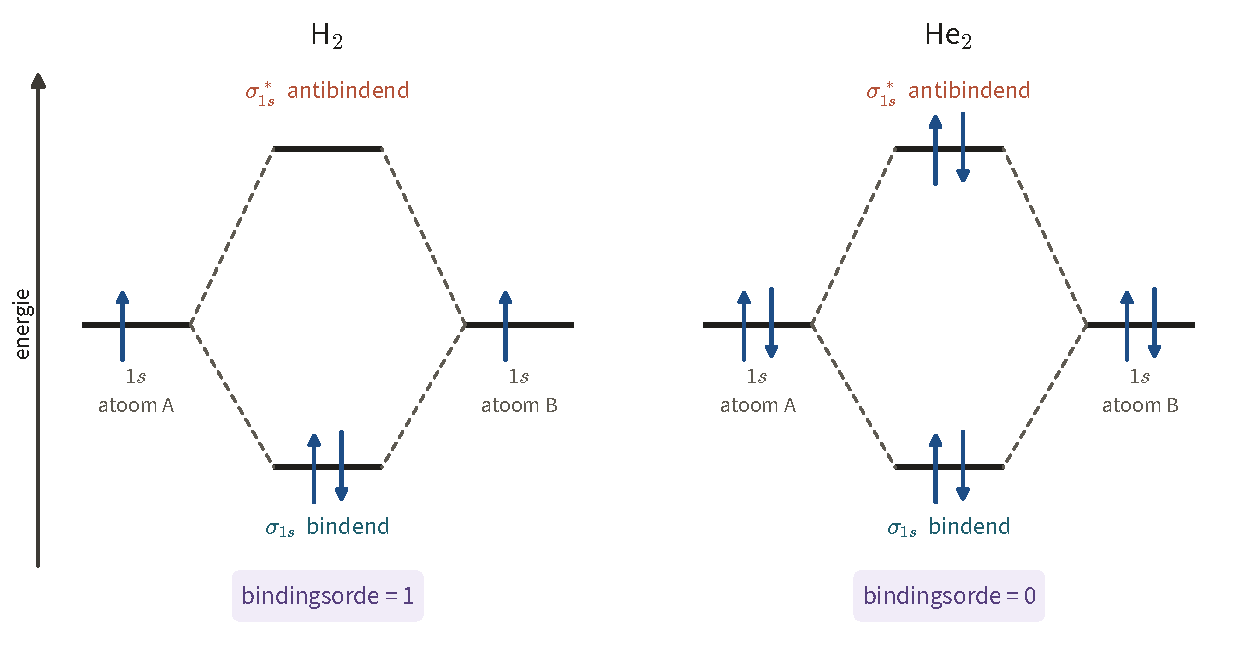
\includegraphics[width=0.62\linewidth]{Figuren/molecuulorbitalen}
    \caption{Molecuulorbitaaldiagram voor \ce{H2} (links) en \ce{He2} (rechts): de twee atomaire $1s$-orbitalen vormen een bindend $\sigma_{1s}$- en een antibindend $\sigma_{1s}^*$-orbitaal.}
    \label{fig:mo-H2}
\end{figure}

\begin{voorbeeld}{Waarom $\mathrm{H_2}$ bestaat en $\mathrm{He_2}$ niet}
In \ce{H2} bezetten de twee elektronen het bindende $\sigma_{1s}$ (figuur~\ref{fig:mo-H2}): bindingsorde $(2-0)/2 = 1$, een enkelvoudige binding. In \ce{He2} moeten de vier elektronen ook $\sigma_{1s}^*$ vullen: bindingsorde $(2-2)/2 = 0$. Bindende en antibindende bijdragen heffen elkaar op, en \ce{He2} bestaat niet als stabiele molecule.
\end{voorbeeld}

\subsection{Bindingsenergie, reactie-enthalpie en bindingslengte}
\label{sec:bindingslengte}

Bij de vorming van een binding komen de elektronen in een lagere energietoestand en wordt het verschil vrijgezet. De reactie-enthalpie is dus het verschil tussen de energie van de bindingen in reagentia en producten: zijn de nieuwe bindingen samen sterker, dan is de reactie exotherm.

Te ver uit elkaar overlappen de golffuncties niet genoeg; te dicht bij elkaar stoten de kernen elkaar af. Bij de \emph{bindingslengte} is de energie minimaal (figuur~\ref{fig:morse-h2}). Die lengte en de kromming van de put bepalen hoe een molecule roteert en vibreert.

\begin{figure}[htb]
    \centering
    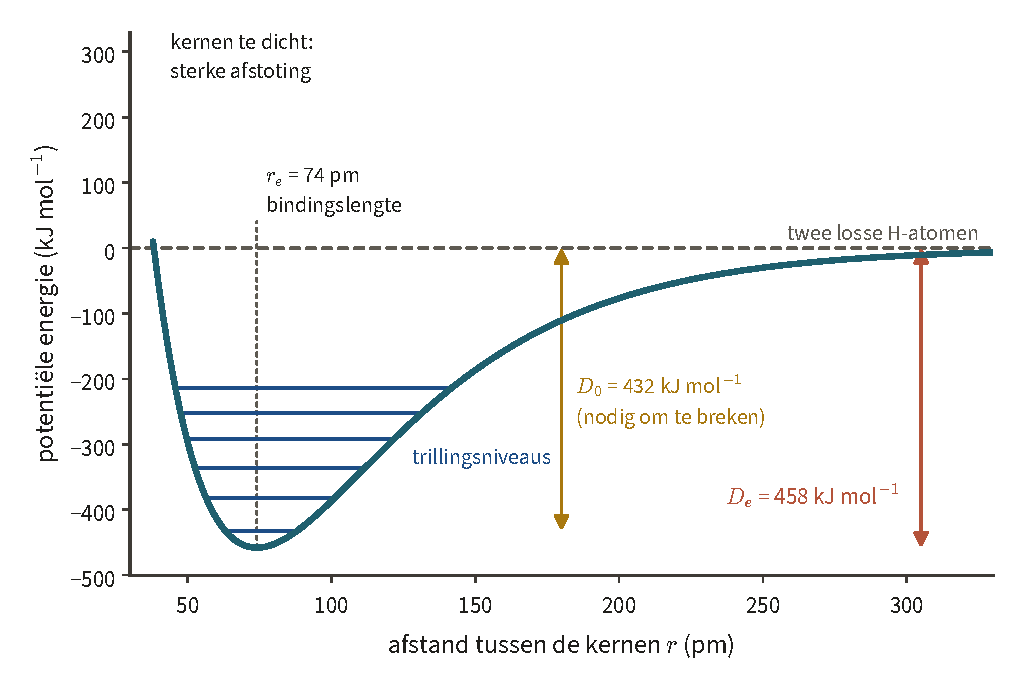
\includegraphics[width=0.62\linewidth]{Figuren/morse_h2}
    \caption{Potentiële energie van \ce{H2} tegen de kernafstand, met minimum bij $r_e = \SI{74}{\pico\metre}$. Door de trillingsenergie (horizontale niveaus) ligt de laagste toestand boven de bodem, zodat de bindingsenergie $D_0$ kleiner is dan de putdiepte $D_e$.}
    \label{fig:morse-h2}
\end{figure}

\begin{casusuitgewerkt}{waarom doet stikstof niets?}
Elk stikstofatoom brengt vijf valentie-elektronen mee ($2s^2\,2p^3$). Uit de acht atomaire orbitalen ($2s$ en drie $2p$ per atoom) ontstaan acht molecuulorbitalen (figuur~\ref{fig:mo-N2}). De tien valentie-elektronen vullen ze van onder naar boven: acht komen in bindende orbitalen ($\sigma_{2s}$, twee $\pi_{2p}$, $\sigma_{2p}$), twee in het antibindende $\sigma^*_{2s}$. De bindingsorde is
\[
\text{bindingsorde} = \frac{8 - 2}{2} = 3:
\]
een drievoudige binding, \'e\'en $\sigma$ en twee $\pi$. Ze is kort (\SI{110}{\pico\metre}) en zeer sterk: \SI{945}{\kilo\joule\per\mole}, bijna drie keer een C--C-binding. Om ze met licht te breken, is een foton van minstens $N_\mathrm{A}hc/\lambda = \SI{945}{\kilo\joule\per\mole}$ nodig, dus $\lambda < \SI{127}{\nano\metre}$: ver ultraviolet, dat de onderste atmosfeer niet bereikt. Bovendien ligt het hoogst bezette orbitaal laag en het laagste lege orbitaal ($\pi^*_{2p}$) hoog, zodat de molecule elektronen moeilijk afgeeft of opneemt. Daarom heeft de ammoniaksynthese een katalysator nodig die de binding helpt verzwakken (hoofdstukken~\ref{ch:grensvlakken} en~\ref{ch:kinetiek}).

\emph{Volgende vraag.} Een binding is geen starre staaf: ze kan trillen, zoals de niveaus in figuur~\ref{fig:morse-h2} tonen. Zowel \ce{N2} als \ce{CO2} heeft sterke bindingen die trillen. Waarom absorbeert dan enkel CO$_2$ infrarood?
\end{casusuitgewerkt}

\begin{figure}[htb]
    \centering
    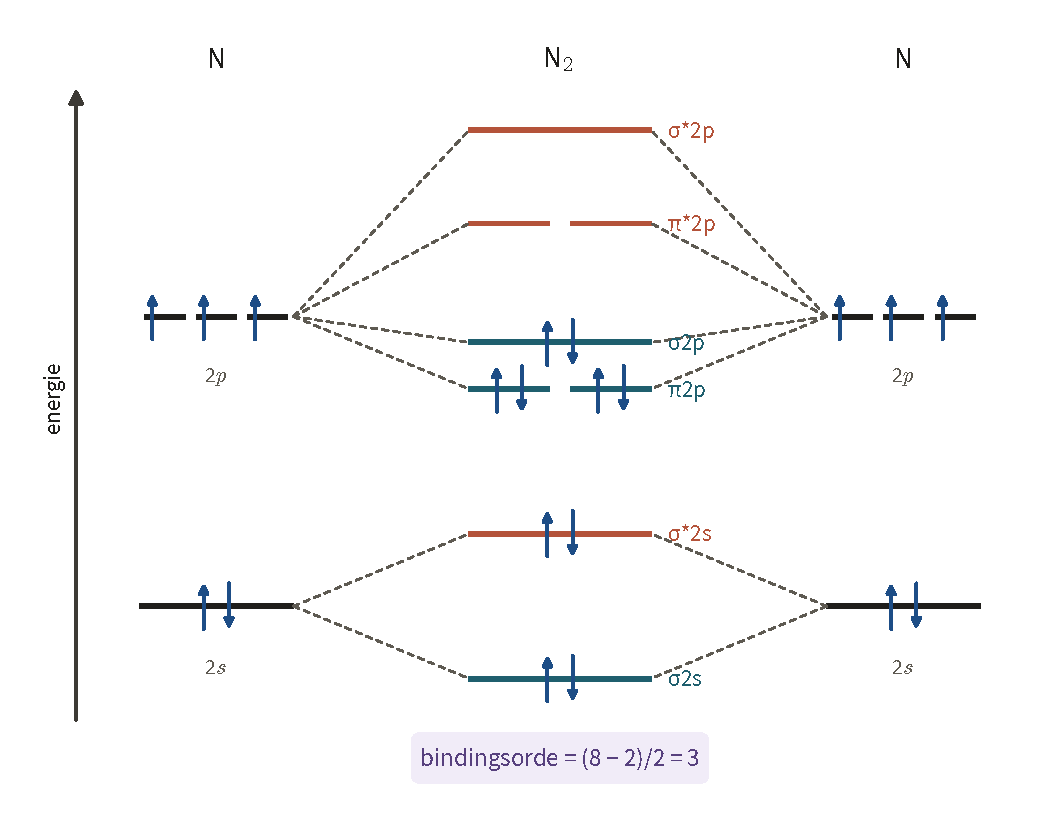
\includegraphics[width=0.7\linewidth]{Figuren/mo_stikstof}
    \caption{Molecuulorbitaaldiagram van \ce{N2} (enkel de valentie-elektronen). Acht elektronen in bindende orbitalen, twee in een antibindend orbitaal: een drievoudige binding. Bij \ce{N2} ligt $\sigma_{2p}$ net boven $\pi_{2p}$; bij \ce{O2} en \ce{F2} is die volgorde omgekeerd.}
    \label{fig:mo-N2}
\end{figure}

\section{Moleculaire beweging en moleculaire spectra}
\label{sec:moleculaire-beweging}

\begin{casus}{CO$_2$ tegenover stikstof}
De drievoudige binding van \ce{N2} trilt, net als de bindingen in CO$_2$. Toch laat stikstof het infrarood van de aarde volledig door, terwijl CO$_2$ het bij \SI{4.3}{} en \SI{15}{\micro\metre} absorbeert. Wat bepaalt of een molecule infrarood licht kan opnemen?

\emph{Schat eerst zelf:} licht is een elektrisch veld dat heen en weer schommelt. Waaraan kan zo'n veld ``trekken'' in een molecule? Is er een verschil tussen \ce{N2}, waarin beide atomen gelijk zijn, en CO$_2$?
\end{casus}

Een molecule kan als geheel door de ruimte bewegen (\emph{translatie}), rond zijn zwaartepunt tollen (\emph{rotatie}) en zijn kernen laten trillen rond de evenwichtsafstand (\emph{vibratie}). Ook die bewegingen volgen de Schr\"odingervergelijking en zijn dus gekwantiseerd, elk met een eigen kwantumgetal. Zo kan een molecule energie opnemen zonder dat een elektron van toestand verandert. Dit verklaart de warmtecapaciteit en vormt de basis van infrarood- en microgolfspectroscopie.

\subsection{Translatie: het deeltje in een doos}
\label{sec:translatie}

De translatie van een molecule in een vat is het deeltje in een doos van \S~\ref{sec:discrete-energieniveaus}, met translationeel kwantumgetal $n_{\mathrm{trans}}$:
\begin{equation}
\boxed{
E_{n_{\mathrm{trans}}} = \frac{n_{\mathrm{trans}}^2 h^2}{8mL^2}, \qquad n_{\mathrm{trans}}=1,2,3,\ldots
}
\end{equation}

\begin{voorbeeld}{Translatieniveaus van \ce{N2} in een vat}
Eén \ce{N2}-molecule ($m=\SI{4.652e-26}{kg}$) in een vat met $L=\SI{0.10}{m}$:
\[
E_1 = \frac{(6.626\times10^{-34})^2}{8(4.652\times10^{-26})(0.10)^2} = \SI{1.18e-40}{J}, \qquad \Delta E_{1\to2} = 3E_1 = \SI{3.54e-40}{J}.
\]
Bij \SI{298}{K} is $k_BT = \SI{4.12e-21}{J}$, zodat $\Delta E/k_BT \approx 10^{-19}$. De translatieniveaus liggen zo dicht bij elkaar dat ze voor alle praktische doeleinden continu zijn.
\end{voorbeeld}

\subsection{Rotatie: de starre rotator}
\label{sec:rotatie}

Een tweeatomige molecule roteert rond een as loodrecht op de binding. In het model van de \emph{starre rotator} zijn twee massa's verbonden door een staaf met de bindingslengte $r$. Met de \emph{gereduceerde massa} $\mu = m_1 m_2/(m_1+m_2)$ en het traagheidsmoment $I = \mu r^2$ levert de Schr\"odingervergelijking het \emph{rotationeel kwantumgetal} $J$:
\begin{equation}
\boxed{
E_J = J(J+1)\frac{\hbar^2}{2I}, \qquad J=0,1,2,\ldots
}
\end{equation}
Elk niveau is $(2J+1)$-voudig \emph{ontaard}: er bestaan $2J+1$ oriëntaties van de rotatie-as met exact dezelfde energie, zoals de drie $p$-orbitalen dezelfde energie hebben.

\begin{voorbeeld}{Rotatieniveaus van HCl}
HCl heeft $r=\SI{127.5}{pm}$, $m_H=\SI{1.008}{u}$ en $m_{Cl}=\SI{34.97}{u}$ ($\SI{1}{u}=\SI{1.6605e-27}{kg}$). Dan is $\mu = \SI{1.628e-27}{kg}$ en $I = \mu r^2 = \SI{2.646e-47}{kg\,m^2}$, zodat
\[
\frac{\hbar^2}{2I} = \frac{(1.0546\times10^{-34})^2}{2(2.646\times10^{-47})} = \SI{2.10e-22}{J}, \qquad \Delta E_{0\to1} = \SI{4.20e-22}{J} \approx 0.10\,k_BT.
\]
Rotatieniveaus liggen dicht genoeg om bij kamertemperatuur ruim bezet te zijn. Overgangen ertussen liggen in het microgolfgebied.
\end{voorbeeld}

\subsection{Vibratie: de harmonische oscillator}
\label{sec:vibratie}

Voor kleine uitwijkingen rond de bindingslengte gedraagt een binding zich als een veer met veerconstante $k$: de \emph{harmonische oscillator}. Het \emph{vibrationeel kwantumgetal} $v$ geeft
\begin{equation}
\boxed{
E_v = \left(v+\frac{1}{2}\right)h\nu, \qquad \nu = \frac{1}{2\pi}\sqrt{\frac{k}{\mu}}, \qquad v=0,1,2,\ldots
}
\end{equation}
Zelfs in de grondtoestand is de energie niet nul maar $\tfrac{1}{2}h\nu$, de \emph{nulpuntsenergie}: een binding trilt altijd, ook bij \SI{0}{K}.

\begin{voorbeeld}{Vibratie van CO}
CO heeft $k=\SI{1902}{N/m}$ en $\mu = \SI{1.139e-26}{kg}$. Dan is
\[
\nu = \frac{1}{2\pi}\sqrt{\frac{1902}{1.139\times10^{-26}}} = \SI{6.50e13}{Hz}, \qquad \tilde\nu = \nu/c = \SI{2168}{cm^{-1}},
\]
dicht bij de gemeten infraroodabsorptie (\SI{2143}{cm^{-1}}). De stap tussen niveaus is $h\nu = \SI{4.31e-20}{J} \approx 10.5\,k_BT$. Slechts één op de $\mathrm{e}^{10.5} \approx 37\,000$ moleculen zit bij kamertemperatuur in $v=1$: vibratie is ``bevroren''. De nulpuntsenergie bedraagt $\tfrac{1}{2}h\nu = \SI{12.97}{kJ/mol}$.
\end{voorbeeld}

De energiestappen van de verschillende bewegingen liggen vele grootteordes uit elkaar:

\begin{center}
\begin{tabular}{lccc}
\toprule
Beweging & Kwantumgetal & Typische $\Delta E$ & Spectraal gebied \\
\midrule
Translatie & $n_{\mathrm{trans}}$ & $\sim 10^{-40}~\mathrm{J}$ ($\ll k_BT$) & quasi-continu \\
Rotatie & $J$ & $\sim 10^{-22}$--$10^{-21}~\mathrm{J}$ ($\sim k_BT$) & microgolf \\
Vibratie & $v$ & $\sim 10^{-20}~\mathrm{J}$ ($\gg k_BT$) & infrarood \\
Elektronisch & $n,l,m_l,m_s$ & $\sim 10^{-19}$--$10^{-18}~\mathrm{J}$ & zichtbaar/UV \\
\bottomrule
\end{tabular}
\end{center}

Bij stijgende temperatuur worden de bewegingen daarom ``na elkaar'' geactiveerd: bij kamertemperatuur zijn translatie en rotatie volledig actief, vibratie nauwelijks, en elektronische aanslag niet.

\subsection{Moleculaire spectra}
\label{sec:moleculaire-spectra}

Elke overgang tussen twee niveaus absorbeert of zendt een foton uit met $\Delta E = h\nu$. Omdat de energieschalen zo verschillen, vallen de spectra in gescheiden gebieden:
\begin{itemize}
\item \textbf{Rotatiespectra} (microgolf, selectieregel $\Delta J=\pm1$) vereisen een permanent dipoolmoment. \ce{N2} en \ce{O2} hebben dat niet en zijn microgolf-inactief.
\item \textbf{Vibratiespectra} (infrarood, $\Delta v=\pm1$) vereisen dat het dipoolmoment \emph{verandert} tijdens de trilling; waarom, zie je in de casus hieronder. Elke functionele groep heeft een eigen IR-band, wat infraroodspectroscopie het standaardinstrument voor procesanalyse maakt.
\item \textbf{Elektronische spectra} (zichtbaar en UV), bijvoorbeeld een $\pi\to\pi^*$-overgang tussen het hoogst bezette (HOMO) en laagst onbezette molecuulorbitaal (LUMO), verklaren kleur: een stof die een bepaalde golflengte absorbeert, toont de complementaire kleur. UV-Vis-spectroscopie meet zo concentraties via de wet van Lambert--Beer.
\end{itemize}

\begin{casusuitgewerkt}{CO$_2$ tegenover stikstof}
\emph{Stap 1: wat trekt het licht?} Het elektrisch veld van een lichtgolf duwt positieve en negatieve ladingen in tegengestelde richting. Het kan dus enkel energie overdragen aan een trilling als die trilling de ladingsverdeling, het \emph{dipoolmoment}, heen en weer laat schommelen in hetzelfde ritme.

\emph{Stap 2: stikstof.} In \ce{N2} zijn beide atomen gelijk; de elektronen zitten altijd symmetrisch verdeeld. Hoe ver de atomen ook uit elkaar gaan, het dipoolmoment blijft nul. De trilling bestaat (bij \SI{2330}{\per\centi\metre}, ongeveer \SI{4.3}{\micro\metre}), maar het licht kan er niet aan trekken: \ce{N2} is IR-inactief. Hetzelfde geldt voor \ce{O2}.

\emph{Stap 3: CO$_2$.} Een lineaire molecule met drie atomen heeft vier trillingen (figuur~\ref{fig:trillingen-co2}). Zuurstof trekt elektronen sterker aan dan koolstof, zodat elke C=O-binding een eigen dipool heeft. In de rechte molecule heffen beide dipolen elkaar op.
\begin{itemize}
\item Bij de \emph{symmetrische strek} bewegen beide zuurstofatomen tegelijk naar buiten: de dipolen blijven elkaar opheffen. IR-inactief.
\item Bij de \emph{asymmetrische strek} wordt de ene binding langer en de andere korter: er ontstaat een schommelende dipool langs de as. IR-actief bij \SI{2349}{\per\centi\metre}, of $\lambda = 1/\tilde\nu = \SI{4.26}{\micro\metre}$: de lijn van de CO$_2$-meter.
\item Bij de \emph{buiging} (in twee loodrechte richtingen, dus twee keer) knikt de molecule: er ontstaat een dipool loodrecht op de as. IR-actief bij \SI{667}{\per\centi\metre}, of \SI{15.0}{\micro\metre}.
\end{itemize}

\emph{Stap 4: waarom de buiging het klimaat bepaalt.} De buiging absorbeert bij \SI{15}{\micro\metre}, vlak naast het maximum van de straling van de aarde (\SI{10}{\micro\metre}, figuur~\ref{fig:zon-aarde}). De asymmetrische strek bij \SI{4.3}{\micro\metre} valt in een gebied waar de aarde nauwelijks straalt; ze is ideaal voor een meettoestel, maar speelt in het klimaat een kleine rol. De energie van een buigingsfoton is $N_\mathrm{A}hc\tilde\nu = \SI{8.0}{\kilo\joule\per\mole}$, slechts drie keer $RT$ bij \SI{15}{\celsius}.

\emph{Volgende vraag.} Bij \SI{15}{\celsius} is $RT = \SI{2.4}{\kilo\joule\per\mole}$, niet zo veel kleiner dan de \SI{8.0}{\kilo\joule\per\mole} van de buiging. Trillen sommige CO$_2$-moleculen dan al vanzelf, zonder licht? En wat betekent dat voor de warmte die het gas opneemt?
\end{casusuitgewerkt}

\begin{figure}[htb]
    \centering
    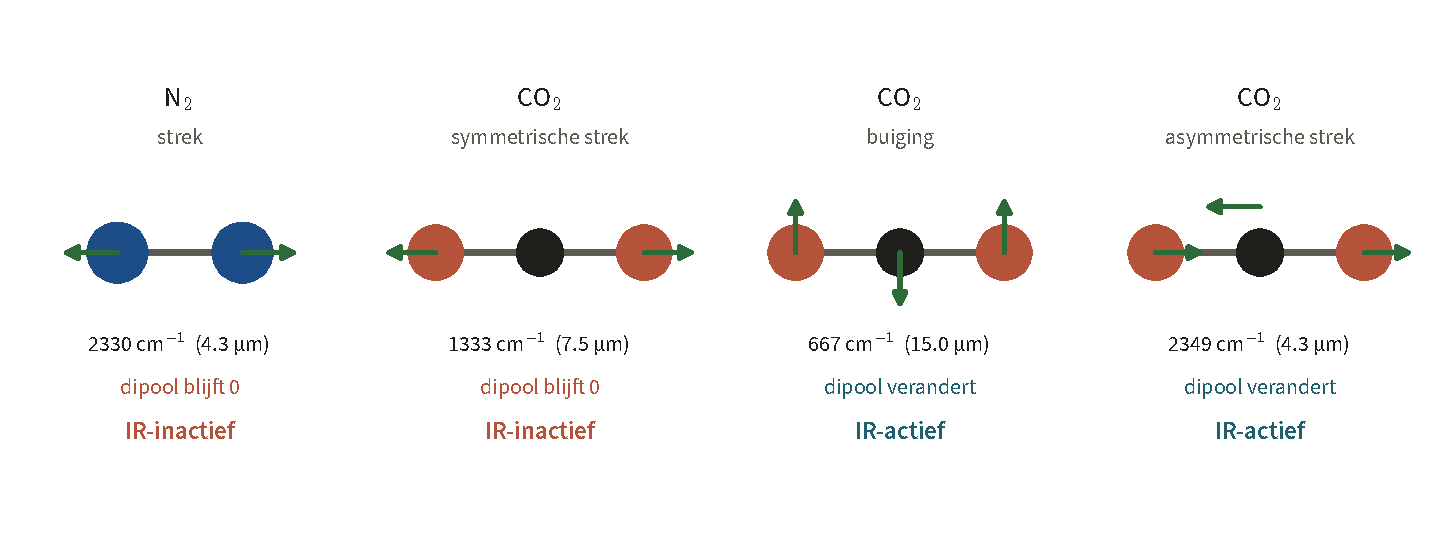
\includegraphics[width=\linewidth]{Figuren/trillingen_co2}
    \caption{De trilling van \ce{N2} en de trillingen van CO$_2$ (de buiging komt twee keer voor, in twee loodrechte vlakken). Enkel trillingen die het dipoolmoment doen veranderen, absorberen infrarood. Golfgetallen: NIST; de symmetrische strek van CO$_2$ is een gemiddelde van twee gekoppelde banden (1285 en \SI{1388}{\per\centi\metre}).}
    \label{fig:trillingen-co2}
\end{figure}

\section{Van kwantumtoestanden naar thermodynamica}
\label{sec:kwantum-thermo}

\begin{casus}{waarom neemt CO$_2$ meer warmte op?}
Bij \SI{25}{\celsius} is $C_{p,\mathrm{m}} = \SI{29.1}{\joule\per\mole\per\kelvin}$ voor stikstof en \SI{37.1}{\joule\per\mole\per\kelvin} voor CO$_2$ (tabel~\ref{tab:cp_coeff}). Beide zijn lineaire moleculen die even vrij bewegen en draaien. Waar komt het verschil van \SI{8}{\joule\per\mole\per\kelvin} vandaan? En hoeveel CO$_2$-moleculen in de atmosfeer trillen al bij \SI{15}{\celsius}?

\emph{Schat eerst zelf:} welke beweging heeft CO$_2$ die stikstof bij kamertemperatuur niet kan aanslaan? Kijk naar de golfgetallen in figuur~\ref{fig:trillingen-co2}.
\end{casus}

\subsection{De Boltzmannverdeling}
\label{sec:boltzmannverdeling}

Een mol gas bevat $6\times10^{23}$ moleculen. De vraag is dus niet in welk niveau \emph{één} molecule zit, maar hoeveel moleculen gemiddeld in elk niveau zitten. In thermisch evenwicht geldt voor twee niveaus met energieverschil $\Delta E = E_i - E_j$ de \emph{Boltzmannverdeling}:
\begin{equation}
\boxed{\frac{N_i}{N_j} = \frac{g_i}{g_j}\,\exp\!\left(-\frac{\Delta E}{k_\mathrm{B}T}\right)}
\label{eq:boltzmann}
\end{equation}
met $k_\mathrm{B} = \SI{1.381e-23}{\joule\per\kelvin}$ en $g_i$ de ontaarding (voor vibratieniveaus $g = 1$). Per mol schrijf je $\Delta E_\mathrm{m}/RT$, want $R = N_\mathrm{A}k_\mathrm{B}$. We leiden de verdeling hier niet af, maar de betekenis is eenvoudig: $k_\mathrm{B}T$ is de typische thermische energie die een molecule bij botsingen uitwisselt ($RT = \SI{2.48}{\kilo\joule\per\mole}$ bij \SI{298}{\kelvin}).
\begin{itemize}
\item $\Delta E \ll k_\mathrm{B}T$: beide niveaus zijn bijna even sterk bezet; de beweging gedraagt zich klassiek (translatie, rotatie).
\item $\Delta E \gg k_\mathrm{B}T$: het hogere niveau is vrijwel leeg; de beweging is ``bevroren'' (vibratie bij kamertemperatuur).
\item Een hogere temperatuur bevolkt hogere niveaus, maar het laagste blijft altijd het sterkst bezet (bij gelijke $g$).
\end{itemize}

\begin{voorbeeld}{Vibrerende stikstof in een vlam}
De vibratie van \ce{N2} ($\tilde\nu = \SI{2330}{\per\centi\metre}$) heeft $\Delta E = hc\tilde\nu = \SI{4.63e-20}{\joule}$. Bij \SI{300}{\kelvin} is $\Delta E/k_\mathrm{B}T = 11.2$ en $N_1/N_0 = 1.4\times10^{-5}$. Bij \SI{2000}{\kelvin} is $\Delta E/k_\mathrm{B}T = 1.68$ en $N_1/N_0 = 0.19$: bijna één op vijf moleculen vibreert. Daarom stijgt $C_p$ van stikstof van \SI{29.1}{} naar \SI{36}{\joule\per\mole\per\kelvin}, en moesten we voor de vlamtemperatuur in hoofdstuk~\ref{ch:energie} met een temperatuurafhankelijke $C_p$ rekenen.
\end{voorbeeld}

\begin{toepassing}{De luchtdruk op de berg}
De Boltzmannverdeling geldt voor elke vorm van energie, ook voor de potentiële energie $Mgh$ per mol in het zwaartekrachtveld. De druk daalt daarom exponentieel met de hoogte:
\begin{equation}
p(h) = p_0 \exp\!\left(-\frac{Mgh}{RT}\right).
\end{equation}
Met $M = \SI{0.029}{\kilo\gram\per\mole}$ en $T \approx \SI{273}{\kelvin}$ daalt de druk met een factor $\mathrm{e}$ per \SI{8}{\kilo\metre}. Op de Mont Blanc (\SI{4808}{\metre}) is de druk ongeveer \SI{0.55}{\bar}, op de Everest (\SI{8849}{\metre}) \SI{0.33}{\bar}. Water kookt daar al bij ongeveer \SI{70}{\celsius} (hoofdstuk~\ref{ch:niet-reagerend}).
\end{toepassing}

\subsection{Warmtecapaciteit}

In hoofdstuk~\ref{ch:energie} was $C_{V,m}$ een experimenteel gegeven: ongeveer $\tfrac{3}{2}R$ voor een eenatomig gas en $\tfrac{5}{2}R$ voor een tweeatomig gas bij kamertemperatuur. Nu kunnen we dat verklaren. Volgens de \emph{equipartitiestelling} draagt elke bewegingsrichting die klassiek toegankelijk is ($\Delta E \ll k_BT$) $\tfrac{1}{2}R$ per mol bij.
\begin{itemize}
\item Een eenatomig gas transleert in drie richtingen: $C_{V,m}=\tfrac{3}{2}R$.
\item Een lineair tweeatomig gas roteert bovendien rond twee assen (rotatie rond de bindingsas telt niet): $C_{V,m}=\tfrac{5}{2}R = \SI{20.8}{J/(mol\,K)}$. Voor CO is de gemeten waarde \SI{20.2}{J/(mol\,K)}.
\item Vibratie draagt pas bij als $k_BT$ vergelijkbaar wordt met $h\nu$, en dan met $R$ per trilling (kinetische plus potentiële energie). $C_{V,m}$ stijgt daardoor geleidelijk naar $\tfrac{7}{2}R$.
\end{itemize}

Hoe groot die bijdrage van een trilling precies is, volgt uit de Boltzmannverdeling. We geven het resultaat zonder afleiding; het hangt enkel af van de verhouding $x = h\nu/k_\mathrm{B}T$:
\begin{equation}
C_{V,\mathrm{vib}} = R\,\frac{x^2\,\mathrm{e}^{x}}{(\mathrm{e}^{x}-1)^2}, \qquad x = \frac{h\nu}{k_\mathrm{B}T} = \frac{hc\tilde\nu}{k_\mathrm{B}T}.
\label{eq:cv-vib}
\end{equation}
Bij lage temperatuur ($x \gg 1$) is de bijdrage nul, bij hoge temperatuur ($x \ll 1$) nadert ze $R$. Figuur~\ref{fig:cp-co2-n2} toont dat dit eenvoudige model de gemeten warmtecapaciteit van \ce{N2} en CO$_2$ over het hele temperatuurbereik volgt.

\begin{figure}[htb]
    \centering
    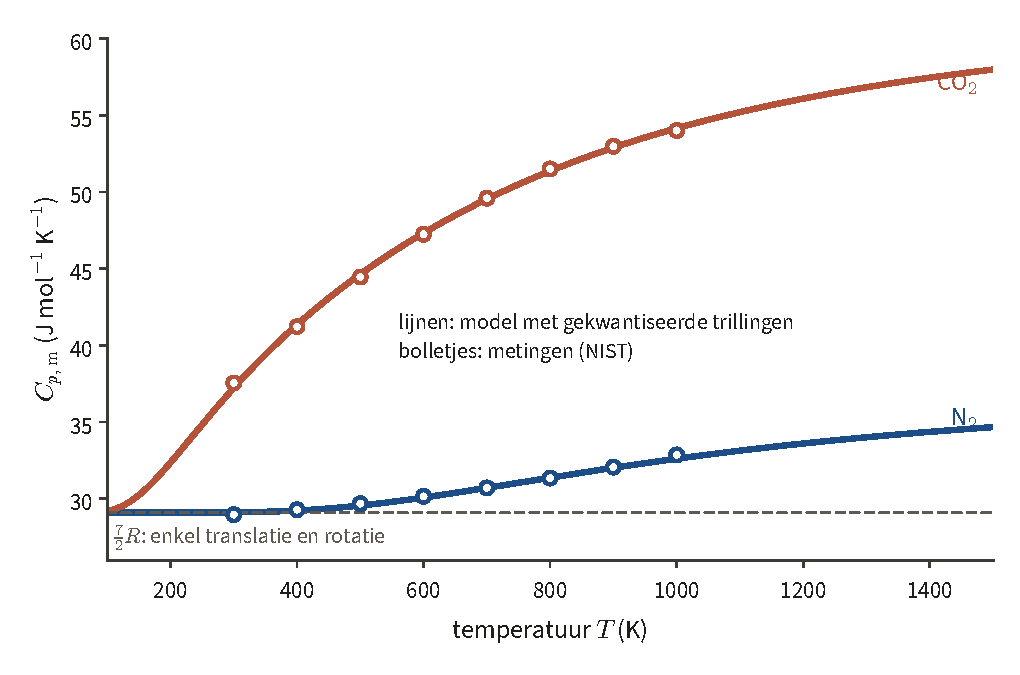
\includegraphics[width=0.7\linewidth]{Figuren/cp_co2_n2}
    \caption{Warmtecapaciteit van \ce{N2} en CO$_2$. Lijnen: $\tfrac72R$ plus de bijdrage~\eqref{eq:cv-vib} van elke trilling (golfgetallen uit figuur~\ref{fig:trillingen-co2}). Bolletjes: correlaties uit tabel~\ref{tab:cp_coeff} (NIST).}
    \label{fig:cp-co2-n2}
\end{figure}

\begin{casusuitgewerkt}{waarom neemt CO$_2$ meer warmte op?}
\emph{Stap 1: hoeveel CO$_2$ trilt?} Voor de buiging ($\tilde\nu = \SI{667}{\per\centi\metre}$) is bij \SI{288}{\kelvin}
\[
x = \frac{hc\tilde\nu}{k_\mathrm{B}T} = \frac{(6.626\times10^{-34})(2.998\times10^{10})(667)}{(1.381\times10^{-23})(288)} = 3.33,
\qquad
\frac{N_1}{N_0} = 2\,\mathrm{e}^{-3.33} = 0.071.
\]
De factor 2 is de ontaarding: de molecule kan in twee loodrechte vlakken buigen. Zeven procent van de CO$_2$-moleculen buigt dus al door de botsingen met andere moleculen. Zo'n trillende molecule kan haar energie als infraroodfoton uitzenden, in elke richting, ook terug naar de aarde. Daarom houdt CO$_2$ de warmte vast: het absorbeert de straling van de aarde, geeft de energie bij botsingen door aan de lucht, en straalt een deel terug naar beneden. Voor de asymmetrische strek is $x = 11.7$ en trilt slechts \'e\'en molecule op honderdduizend.

\emph{Stap 2: de warmtecapaciteit.} Bij \SI{298}{\kelvin} geeft vergelijking~\eqref{eq:cv-vib} per trilling:
\begin{center}
\begin{tabular}{lccc}
\toprule
Trilling & $\tilde\nu$ (\si{\per\centi\metre}) & $x$ & $C_{V,\mathrm{vib}}$ (\si{\joule\per\mole\per\kelvin}) \\
\midrule
CO$_2$ buiging ($2\times$) & 667 & 3.22 & $2 \times 3.74 = 7.48$ \\
CO$_2$ symmetrische strek & 1333 & 6.43 & 0.56 \\
CO$_2$ asymmetrische strek & 2349 & 11.3 & 0.01 \\
\ce{N2} strek & 2330 & 11.2 & 0.01 \\
\bottomrule
\end{tabular}
\end{center}
Translatie en rotatie geven samen $\tfrac52R$, en $C_p = C_V + R$ (hoofdstuk~\ref{ch:energie}), dus $\tfrac72R = \SI{29.10}{\joule\per\mole\per\kelvin}$ voor elke lineaire molecule. Daarbij komt de bijdrage van de trillingen:
\begin{align*}
C_{p,\mathrm{m}}(\ce{N2}) &= 29.10 + 0.01 = \SI{29.1}{\joule\per\mole\per\kelvin},\\
C_{p,\mathrm{m}}(\ce{CO2}) &= 29.10 + 7.48 + 0.56 + 0.01 = \SI{37.2}{\joule\per\mole\per\kelvin}.
\end{align*}
Gemeten: 29.1 en \SI{37.1}{\joule\per\mole\per\kelvin}. Het hele verschil komt van de zachte buiging van CO$_2$, die als enige trilling al bij kamertemperatuur energie opneemt. Bij hogere temperatuur komen ook de andere trillingen vrij, en daarom stijgt $C_p$ met $T$ (figuur~\ref{fig:cp-co2-n2}): de veelterm uit tabel~\ref{tab:cp_coeff} is geen toevallige curve-fit, maar een gevolg van gekwantiseerde trillingsniveaus.
\end{casusuitgewerkt}

\subsection{Activeringsenergie en overgangstoestand}
\label{sec:activeringsenergie-kwantum}

Tijdens een reactie verdwijnen oude bindingen niet op hetzelfde ogenblik dat nieuwe ontstaan. Het systeem passeert tussentoestanden waarvan sommige een hogere energie hebben dan zowel reagentia als producten. De minimale energie om die \emph{overgangstoestand} te bereiken, is de \emph{activeringsenergie}. Ze verklaart waarom een reactie thermodynamisch gunstig maar toch traag kan zijn: de thermodynamica bepaalt de eindtoestand, de kinetiek hoe snel die bereikt wordt. Enkel moleculen die toevallig genoeg energie bezitten, halen de overgangstoestand. Hoeveel dat er zijn, zegt opnieuw de Boltzmannverdeling.

\subsection{Waarom reacties sneller gaan bij hogere temperatuur}

Een reactie verloopt enkel als botsende moleculen minstens de activeringsenergie $E_\mathrm{a}$ bezitten. Die fractie volgt uit dezelfde Boltzmannfactor, $\exp(-E_\mathrm{a}/RT)$. Voor $E_\mathrm{a} = \SI{50}{\kilo\joule\per\mole}$ is ze bij \SI{35}{\celsius} een factor
\[
\exp\!\left[\frac{50\,000}{8.314}\left(\frac{1}{298.15} - \frac{1}{308.15}\right)\right] = 1.9
\]
groter dan bij \SI{25}{\celsius}. Dat is de oorsprong van de vuistregel ``twee keer sneller per \SI{10}{\celsius}'' en van de wet van Arrhenius (hoofdstuk~\ref{ch:kinetiek}). Een koelkast vertraagt bederfreacties volgens hetzelfde principe.

\section{Het broeikaseffect opnieuw bekeken}

Met de begrippen uit dit hoofdstuk kan je de vragen uit het begin beantwoorden:
\begin{itemize}
\item \emph{Zon en aarde} (\S\ref{sec:licht-pakketjes}): de kleur van de straling volgt uit de temperatuur (wet van Wien). Zonlicht heeft fotonen van zo'n \SI{240}{\kilo\joule\per\mole}, het infrarood van de aarde slechts \SI{12}{\kilo\joule\per\mole}: genoeg om moleculen te laten trillen, niet om bindingen te breken. Zonder broeikasgassen zou de aarde \SI{-18}{\celsius} zijn.
\item \emph{Scherpe lijnen} (\S\ref{sec:lijnenspectra}): een molecule absorbeert enkel fotonen met $h\nu = \Delta E$ tussen twee toegelaten niveaus. Bij \SI{4.26}{\micro\metre} hoort \SI{28}{\kilo\joule\per\mole}, te weinig voor een elektronische overgang.
\item \emph{Stikstof} (\S\ref{sec:molecuulorbitalen}): een drievoudige binding met bindingsorde 3 en \SI{945}{\kilo\joule\per\mole}; daarom is stikstof zo inert en heeft de ammoniaksynthese een katalysator nodig.
\item \emph{CO$_2$ tegenover stikstof} (\S\ref{sec:moleculaire-beweging}): enkel trillingen die het dipoolmoment doen veranderen, absorberen infrarood. \ce{N2} en \ce{O2} hebben er geen, CO$_2$ heeft er twee: de buiging bij \SI{15}{\micro\metre} (klimaat) en de asymmetrische strek bij \SI{4.26}{\micro\metre} (CO$_2$-meter).
\item \emph{Warmtecapaciteit} (\S\ref{sec:kwantum-thermo}): de zachte buiging van CO$_2$ wordt al bij kamertemperatuur aangeslagen; ze verklaart \SI{8}{\joule\per\mole\per\kelvin} extra warmtecapaciteit en de \SI{7}{\percent} trillende CO$_2$-moleculen die infrarood terugstralen.
\end{itemize}
Dezelfde redeneringen gelden voor elk molecule: waterdamp en methaan zijn broeikasgassen om dezelfde reden als CO$_2$, en de infraroodbanden van functionele groepen maken infraroodspectroscopie tot een standaardinstrument in labo en procescontrole.

Eén vraag blijft open: waarom verlopen sommige processen spontaan in één richting, ook als de energie geen uitsluitsel geeft? Het antwoord ligt in het \emph{aantal manieren} waarop energie en moleculen over de toestanden verdeeld kunnen worden: de entropie van hoofdstuk~\ref{ch:spontaniteit}.

\section{Oefeningen}

% Oefeningen bij dit hoofdstuk (ingevoegd achteraan het hoofdstuk met \input).
% Een oefening:  \begin{oefening} ... \end{oefening}   (boek en website)
% De oplossing:  \begin{oplossing} ... \end{oplossing}       (enkel website, dichtgeklapt)

Constanten: $h = \SI{6.626e-34}{\joule\second}$, $c = \SI{2.998e8}{\metre\per\second}$, $k_B = \SI{1.381e-23}{\joule\per\kelvin}$, $m_e = \SI{9.109e-31}{\kilogram}$, $\SI{1}{\electronvolt} = \SI{1.602e-19}{\joule}$, $1\,\mathrm{u} = \SI{1.6605e-27}{\kilogram}$, $N_A = \SI{6.022e23}{\per\mole}$.

\begin{oefening}
Cesium heeft een elektronenbindingsenergie (werkfunctie) van \(1.95\,\mathrm{eV}\).

\begin{enumerate}
\item[(a)]
  Bereken de minimale frequentie en golflengte van licht die nodig is om elektronen uit een cesiumoppervlak los te slaan.
\item[(b)]
  Wordt zichtbaar licht (ca. \(400\)--\(700\,\mathrm{nm}\)) hiervoor gebruikt? Of eerder UV?
\item[(c)]
  Bereken de maximale kinetische energie van de losgeslagen elektronen wanneer cesium wordt belicht met licht van \(\lambda = 400\,\mathrm{nm}\).
\end{enumerate}

\emph{Hint:} gebruik \(E_{\text{foton}} = h\nu = hc/\lambda\) en \(1~\mathrm{eV} = 1.602\times10^{-19}\,\mathrm{J}\).
\end{oefening}
\begin{oplossing}
\textbf{Resultaat:} (a) \(\nu_0\) = \textbf{4.71\ensuremath{\cdot{}}10\ensuremath{^{14}} Hz}, \(\lambda_0\) = \textbf{636 nm}. (b) Zichtbaar licht volstaat (alles onder 636 nm). (c) \(E_{k,\max}\) = \textbf{1.15 eV} (1.84\ensuremath{\cdot{}}10\ensuremath{^{-19}} J).

\textbf{(a)} De drempelfrequentie volgt uit \(h\nu_0 = \phi\):

\[
\nu_0 = \frac{(1.95)(1.602\times10^{-19})}{6.626\times10^{-34}} = 4.71\times10^{14}\,\mathrm{Hz}, \qquad \lambda_0 = \frac{c}{\nu_0} = 636\,\mathrm{nm}
\]

\textbf{(b)} Alle licht met \(\lambda < 636\,\mathrm{nm}\) maakt elektronen vrij: dat is het grootste deel van het zichtbare spectrum (violet tot oranje). Zichtbaar licht volstaat dus; UV is niet nodig. Daarom werd cesium (en cesiumverbindingen) gebruikt in fotocellen en fotomultiplicatoren voor zichtbaar licht.

\textbf{(c)} \(E_{\text{foton}} = hc/\lambda = 3.10\,\mathrm{eV}\), dus \(E_{k,\max} = 3.10 - 1.95 = 1.15\,\mathrm{eV} = 1.84\times10^{-19}\,\mathrm{J}\).
\end{oplossing}

\begin{oefening}
De energieniveaus van het waterstofatoom worden gegeven door \(E_n = -13.6~\mathrm{eV}/n^2\).

\begin{enumerate}
\item[(a)]
  Bereken de energie van de overgang \(n=3 \to n=2\) (Balmer-reeks) en de golflengte van het uitgezonden foton.
\item[(b)]
  Vergelijk met de overgang \(n=2 \to n=1\) (Lyman-reeks). Welke reeks ligt in het zichtbare gebied?
\item[(c)]
  Hoeveel energie is minimaal nodig om een elektron uit de grondtoestand volledig te ioniseren (tot \(n \to \infty\))?
\end{enumerate}
\end{oefening}
\begin{oplossing}
\textbf{Resultaat:} (a) \(\Delta E\) = \textbf{1.89 eV}, \(\lambda\) = \textbf{656 nm} (rood). (b) \textbf{10.2 eV}, \textbf{122 nm} (UV): de Balmer-reeks is zichtbaar. (c) \textbf{13.6 eV} (1312 kJ/mol).

\textbf{(a)} \(\Delta E = 13.6\left(\frac{1}{4} - \frac{1}{9}\right) = 1.89\,\mathrm{eV}\), zodat \(\lambda = hc/\Delta E = 656\,\mathrm{nm}\): de rode H\(_\alpha\)-lijn.

\textbf{(b)} \(\Delta E = 13.6\left(1 - \frac{1}{4}\right) = 10.2\,\mathrm{eV}\), zodat \(\lambda = 122\,\mathrm{nm}\) (UV). De Balmer-reeks (eindniveau \(n = 2\)) ligt in het zichtbare gebied; de Lyman-reeks (\(n = 1\)) volledig in het UV.

\textbf{(c)} \(E_{\text{ion}} = 0 - (-13.6) = 13.6\,\mathrm{eV}\), of \(1312\,\mathrm{kJ/mol}\).
\end{oplossing}

\begin{oefening}
Beschouw de synthese van waterstofchloride uit de elementen:

\[
\mathrm{H_2(g) + Cl_2(g) \rightarrow 2\,HCl(g)}.
\]

Gebruik de volgende gemiddelde bindingsenergieën:

\begin{itemize}
\item
  \(D(\mathrm{H{-}H}) = 436\,\mathrm{kJ/mol}\)
\item
  \(D(\mathrm{Cl{-}Cl}) = 243\,\mathrm{kJ/mol}\)
\item
  \(D(\mathrm{H{-}Cl}) = 431\,\mathrm{kJ/mol}\)
\end{itemize}

Gevraagd:

\begin{enumerate}
\item[(a)]
  Bereken de reactie-enthalpie uit de bindingsenergieën.
\item[(b)]
  Vergelijk met de waarde die men via standaardvormingsenthalpieën zou krijgen (\(\Delta H_f^\circ(\mathrm{HCl,g}) = -92.3\,\mathrm{kJ/mol}\)). Verklaar eventuele verschillen.
\item[(c)]
  Waarom is deze benadering met gemiddelde bindingsenergieën slechts een schatting?
\end{enumerate}
\end{oefening}
\begin{oplossing}
\textbf{Resultaat:} (a) \(\Delta_r H \approx\) \textbf{\ensuremath{-}183 kJ} per 2 mol HCl. (b) Via vormingsenthalpieën \textbf{\ensuremath{-}184.6 kJ}: minder dan 1 \% verschil. (c) Gemiddelde bindingsenergieën negeren de chemische omgeving (fout typisch 10--30 kJ/mol).

\textbf{(a)} Verbroken: één H--H en één Cl--Cl; gevormd: twee H--Cl.

\[
\Delta_r H \approx 436 + 243 - 2(431) = -183\,\mathrm{kJ}\ \text{(per 2 mol HCl)}
\]

\textbf{(b)} Via vormingsenthalpieën: \(\Delta_r H^\circ = 2(-92.3) = -184.6\,\mathrm{kJ}\). Het verschil is minder dan 1 \%. Dat is hier zo goed omdat het om tweeatomige moleculen gaat: de gebruikte \(D\)-waarden zijn dan geen gemiddelden over veel verbindingen maar de werkelijke dissociatie-energieën van precies deze moleculen. Het kleine restverschil komt van afrondingen en van het feit dat bindingsenergieën en vormingsenthalpieën niet bij exact dezelfde referentietemperatuur gedefinieerd zijn.

\textbf{(c)} In polyatomische moleculen hangt de sterkte van een binding af van de chemische omgeving: een C--H binding in methaan is niet even sterk als een C--H binding in benzeen. Tabelwaarden zijn gemiddelden over veel verbindingen; bovendien negeren ze resonantie, ringspanning en intermoleculaire krachten (de waarden gelden voor de gasfase). Typische fouten bedragen 10 à 30 kJ/mol.
\end{oplossing}

\begin{oefening}
Geef de volledige elektronenconfiguratie (in termen van orbitalen) van de volgende elementen in hun grondtoestand:

\begin{enumerate}
\item[(a)]
  koolstof (\(Z=6\)),
\item[(b)]
  zuurstof (\(Z=8\)),
\item[(c)]
  natrium (\(Z=11\)).
\end{enumerate}

Verklaar voor zuurstof waarom de twee ongepaarde 2p-elektronen in afzonderlijke orbitalen met parallelle spin worden geplaatst (regel van Hund) en hoe dit verband houdt met het uitsluitingsprincipe van Pauli.
\end{oefening}
\begin{oplossing}
\textbf{Resultaat:} C: \textbf{1s\ensuremath{^{2}} 2s\ensuremath{^{2}} 2p\ensuremath{^{2}}}; O: \textbf{1s\ensuremath{^{2}} 2s\ensuremath{^{2}} 2p\ensuremath{^{4}}}; Na: \textbf{{[}Ne{]} 3s\ensuremath{^{1}}}. Zuurstof heeft \textbf{twee ongepaarde 2p-elektronen} met parallelle spin (Hund + Pauli).

\textbf{(a)} C: \(1s^2\,2s^2\,2p^2\). \textbf{(b)} O: \(1s^2\,2s^2\,2p^4\). \textbf{(c)} Na: \(1s^2\,2s^2\,2p^6\,3s^1\), of \([\mathrm{Ne}]\,3s^1\).

Zuurstof heeft vier 2p-elektronen over drie 2p-orbitalen: één orbitaal bevat een elektronenpaar, de twee overige bevatten elk één ongepaard elektron met parallelle spin. Volgens het uitsluitingsprincipe van Pauli kunnen twee elektronen enkel hetzelfde orbitaal delen als hun spins tegengesteld zijn. Elektronen met parallelle spin worden dus gedwongen in verschillende orbitalen, ruimtelijk verder van elkaar, wat hun onderlinge afstoting verlaagt. Daarom is de toestand met maximale totale spin (regel van Hund) energetisch het gunstigst. De twee ongepaarde elektronen verklaren mee waarom zuurstof twee bindingen vormt (zoals in \(\mathrm{H_2O}\)).
\end{oplossing}

\begin{oefening}\label{oef:h2-5}
Een chemische reactie heeft een activeringsenergie van \(150\,\mathrm{kJ/mol}\). Een katalysator verlaagt deze tot \(75\,\mathrm{kJ/mol}\).

\begin{enumerate}
\item[(a)]
  Maak een schematisch energieprofiel (qualitatief) voor de ongekatalyseerde en de gekatalyseerde reactie.
\item[(b)]
  Wat verandert er aan de reactie-enthalpie \(\Delta_r H\) door de katalysator? En aan de evenwichtsconstante?
\item[(c)]
  Hoeveel keer sneller wordt de reactie bij kamertemperatuur (\(298\,\mathrm{K}\)) dankzij de katalysator? Gebruik de Arrhenius-benadering \(k \propto e^{-E_a/RT}\).
\end{enumerate}

\emph{Hint:} bereken de verhouding \(k_{\text{kat}}/k_{\text{onkat}} = \exp\!\bigl((E_{a,\text{onkat}} - E_{a,\text{kat}})/RT\bigr)\).
\end{oefening}
\begin{oplossing}
\textbf{Resultaat:} (b) \(\Delta_r H\) en \(K\) veranderen \textbf{niet}. (c) De reactie wordt ongeveer \textbf{1.4\ensuremath{\cdot{}}10\ensuremath{^{13}} keer} sneller.

\textbf{(a)} Beide profielen starten op hetzelfde niveau (reagentia) en eindigen op hetzelfde niveau (producten). De ongekatalyseerde weg heeft één hoge top (\(150\,\mathrm{kJ/mol}\) boven de reagentia); de gekatalyseerde weg heeft een lagere top (\(75\,\mathrm{kJ/mol}\)), vaak met tussenliggende dalen voor geadsorbeerde tussenproducten.

\textbf{(b)} Niets. \(\Delta_r H\) en \(K\) hangen enkel af van begin- en eindtoestand (toestandsfuncties); een katalysator verandert enkel de weg. Hij versnelt de heen- en terugreactie in dezelfde mate en bereikt hetzelfde evenwicht, alleen sneller.

\textbf{(c)}

\[
\frac{k_{\text{kat}}}{k_{\text{onkat}}} = \exp\!\left(\frac{75\,000}{(8.314)(298)}\right) = e^{30.3} \approx 1.4\times10^{13}
\]

Een reactie die zonder katalysator honderdduizenden jaren zou duren, verloopt nu in minder dan een seconde. Dit is de reden waarom enzymen in je lichaam reacties bij \(37\,^\circ\mathrm{C}\) mogelijk maken.
\end{oplossing}

\begin{oefening}
Wanneer twee golffuncties \(\psi_1\) en \(\psi_2\) worden gecombineerd, ontstaat \(\psi_{\pm} = \psi_1 \pm \psi_2\).

\begin{enumerate}
\item[(a)]
  Schets kwalitatief de waarschijnlijkheidsverdeling \(|\psi_+|^2\) en \(|\psi_-|^2\) in het gebied tussen twee kernen.
\item[(b)]
  Welke van beide correspondeert met een bindende toestand, welke met een antibindende? Verklaar vanuit de gemiddelde kinetische energie.
\item[(c)]
  Waarom wordt in de chemie vrijwel uitsluitend met de bindende toestand gewerkt?
\end{enumerate}
\end{oefening}
\begin{oplossing}
\textbf{Resultaat:} \(\psi_+\) is \textbf{bindend} (verhoogde dichtheid tussen de kernen), \(\psi_-\) is \textbf{antibindend} (knoopvlak tussen de kernen).

\textbf{(a)} \(|\psi_+|^2\) heeft een verhoogde elektronendichtheid tussen de kernen (constructieve interferentie). \(|\psi_-|^2\) heeft halverwege de kernen een knoopvlak waar de dichtheid nul is (destructieve interferentie); de dichtheid zit aan de buitenkant van de kernen.

\textbf{(b)} \(\psi_+\) is bindend, \(\psi_-\) antibindend. In \(\psi_+\) kan het elektron zich over een groter gebied uitspreiden (over beide kernen), wat de golffunctie gladder maakt en de kinetische energie verlaagt; bovendien zit de lading tussen de kernen, waar ze door beide kernen wordt aangetrokken. In \(\psi_-\) dwingt het knoopvlak een sterkere kromming van de golffunctie af (hogere kinetische energie), en de lading tussen de kernen, die ze bij elkaar zou houden, ontbreekt.

\textbf{(c)} In de grondtoestand van stabiele moleculen worden eerst de bindende orbitalen gevuld, omdat die lager in energie liggen. De antibindende orbitalen zijn wel belangrijk voor de bindingsorde (bijvoorbeeld waarom \(\mathrm{He_2}\) niet bestaat), voor aangeslagen toestanden (UV-Vis-spectroscopie, fotochemie) en voor reactiviteit: een reactie breekt een binding vaak door elektronen in een antibindend orbitaal te brengen.
\end{oplossing}

\begin{oefening}
De standaardvormingsenthalpie van waterstofsulfide bedraagt \(\Delta H_f^\circ(\mathrm{H_2S,g}) = -20.6\,\mathrm{kJ/mol}\). De bindingsenergie van een S--H binding bedraagt \(363\,\mathrm{kJ/mol}\) en die van een H--H binding \(436\,\mathrm{kJ/mol}\). Schat hieruit de bindingsenergie van een S--S binding in \(\mathrm{H_2S_2}\), gegeven

\[
\mathrm{2\,H_2S(g) \rightarrow H_2S_2(g) + H_2(g)} \qquad \Delta_r H^\circ \approx +10\,\mathrm{kJ/mol}.
\]

\emph{Hint:} aan de kant van reagentia worden twee S--H bindingen verbroken; aan de kant van producten worden één S--S en één H--H binding gevormd.
\end{oefening}
\begin{oplossing}
\textbf{Resultaat:} \(D(\mathrm{S{-}S})\) \ensuremath{\approx{}} \textbf{280 kJ/mol} (literatuur ca. 265 kJ/mol).

\(\mathrm{H_2S_2}\) (\(\mathrm{H{-}S{-}S{-}H}\)) bevat zelf nog twee S--H bindingen, zodat netto twee S--H bindingen verbroken en één S--S en één H--H binding gevormd worden:

\[
\Delta_r H^\circ = 2D(\mathrm{S{-}H}) - D(\mathrm{S{-}S}) - D(\mathrm{H{-}H})
\]

\[
D(\mathrm{S{-}S}) = 2(363) - 436 - 10 = 280\,\mathrm{kJ/mol}
\]

De literatuurwaarde voor een S--S enkelvoudige binding ligt rond \(265\,\mathrm{kJ/mol}\). S--S bruggen (disulfidebruggen) zijn veel zwakker dan C--C bindingen; dat is waarom ze bij het vulkaniseren van rubber en in het permanent krullen of ontkrullen van haar (keratine) relatief gemakkelijk verbroken en opnieuw gevormd kunnen worden. De gegeven \(\Delta H_f^\circ(\mathrm{H_2S})\) is voor deze berekening niet nodig.
\end{oplossing}

\begin{oefening}
Vergelijk drie soorten straling: UV-B-licht (\(\lambda = 300\,\mathrm{nm}\)), groen licht (\(550\,\mathrm{nm}\)) en de microgolven van een microgolfoven (\(\nu = 2.45\,\mathrm{GHz}\)).

\begin{enumerate}
\item[(a)]
  Bereken voor elk de energie per foton en per mol fotonen.
\item[(b)]
  Een C--C binding heeft een bindingsenergie van ongeveer \(350\,\mathrm{kJ/mol}\). Welke straling kan in principe bindingen in je huid (DNA, eiwitten) breken?
\item[(c)]
  Waarom warmt een microgolfoven je eten wel op, terwijl zijn fotonen zo weinig energie hebben?
\end{enumerate}
\end{oefening}
\begin{oplossing}
\textbf{Resultaat:} (a) UV-B \textbf{399 kJ/mol}, groen \textbf{218 kJ/mol}, microgolf \textbf{0.001 kJ/mol}. (b) Enkel \textbf{UV-B} kan C--C bindingen breken. (c) Microgolven brengen watermoleculen in \textbf{rotatie}; die energie wordt warmte.

\textbf{(a)} Met \(E = hc/\lambda\) en \(E_{\text{mol}} = N_A E\):

\begin{center}
\begin{tabular}{lll}
\toprule
Straling & \(E\) per foton (J) & per mol (kJ/mol) \\
\midrule
UV-B, 300 nm & \(6.62\times10^{-19}\) & 399 \\
Groen, 550 nm & \(3.61\times10^{-19}\) & 218 \\
Microgolf, 2.45 GHz (\(\lambda = 12.2\,\mathrm{cm}\)) & \(1.62\times10^{-24}\) & 0.001 \\
\bottomrule
\end{tabular}
\end{center}

\textbf{(b)} Enkel UV-B levert per foton meer energie dan nodig is om een C--C binding te breken. Daarom veroorzaakt UV zonnebrand en DNA-schade, terwijl zichtbaar licht dat niet doet, hoe fel het ook is: het gaat om de energie per foton, niet om de totale lichtintensiteit (net zoals bij het foto-elektrisch effect).

\textbf{(c)} Microgolffotonen breken geen bindingen. Ze brengen polaire watermoleculen in rotatie (rotatieniveaus liggen in het microgolfgebied). Door botsingen met de omgeving wordt die rotatie-energie omgezet in ongeordende thermische beweging: warmte. Het grote aantal fotonen maakt het verschil.
\end{oplossing}

\begin{oefening}
\begin{enumerate}
\item[(a)]
  Bereken de de Broglie-golflengte van een elektron dat versneld wordt over een spanning van \(100\,\mathrm{V}\) en van \(100\,\mathrm{kV}\) (zoals in een transmissie-elektronenmicroscoop). Gebruik \(E_k = eV = p^2/(2m_e)\) (niet-relativistisch).
\item[(b)]
  Vergelijk met de golflengte van zichtbaar licht (ca. \(500\,\mathrm{nm}\)). Waarom kan je met een elektronenmicroscoop individuele atomen zien en met een lichtmicroscoop niet?
\item[(c)]
  Bereken de de Broglie-golflengte van een tennisbal (\(57\,\mathrm{g}\)) aan \(50\,\mathrm{m/s}\). Waarom merken we in het dagelijks leven niets van het golfkarakter van materie?
\end{enumerate}
\end{oefening}
\begin{oplossing}
\textbf{Resultaat:} (a) \(\lambda\) = \textbf{0.123 nm} (100 V) en \textbf{0.0039 nm} (100 kV). (b) Kleiner dan een atoom, licht is duizenden keren groter. (c) Tennisbal: \(\lambda\) = \textbf{2.3\ensuremath{\cdot{}}10\ensuremath{^{-34}} m}.

\textbf{(a)} \(\lambda = h/p = h/\sqrt{2m_e eV}\).

\begin{itemize}
\item
  \(100\,\mathrm{V}\): \(\lambda = 1.23\times10^{-10}\,\mathrm{m} = 0.123\,\mathrm{nm}\).
\item
  \(100\,\mathrm{kV}\): \(\lambda = 3.9\times10^{-12}\,\mathrm{m} = 0.0039\,\mathrm{nm}\) (relativistisch is het \(3.7\,\mathrm{pm}\); de orde van grootte verandert niet).
\end{itemize}

\textbf{(b)} Het oplossend vermogen van een microscoop is van de orde van de golflengte. Atomen zijn ongeveer \(0.1\)--\(0.3\,\mathrm{nm}\) groot: duizenden keren kleiner dan zichtbaar licht, maar groter dan de golflengte van snelle elektronen. Elektronenmicroscopen worden in de materiaalkunde gebruikt om kristaldefecten, katalysatordeeltjes en nanostructuren te bekijken.

\textbf{(c)} \(\lambda = h/(mv) = 6.626\times10^{-34}/(0.057 \times 50) = 2.3\times10^{-34}\,\mathrm{m}\): ruim \(10^{19}\) keer kleiner dan een atoomkern. Er bestaat geen opening of obstakel waarop zo'n golf merkbaar kan buigen of interfereren. Golfgedrag wordt pas zichtbaar wanneer \(\lambda\) vergelijkbaar is met de afmetingen van het systeem, en dat is enkel zo voor zeer lichte deeltjes op atomaire schaal.
\end{oplossing}

\begin{oefening}
In een molecule met geconjugeerde dubbele bindingen kunnen de \ensuremath{\pi{}}-elektronen zich vrij over de volledige keten bewegen. Een eenvoudig model behandelt ze als deeltjes in een ééndimensionale doos met lengte \(L\), waarin elk niveau twee elektronen bevat (Pauli).

\begin{enumerate}
\item[(a)]
  1,3,5-Hexatriëen (\(\mathrm{CH_2{=}CH{-}CH{=}CH{-}CH{=}CH_2}\)) heeft 6 \ensuremath{\pi{}}-elektronen. Welke niveaus zijn het HOMO en het LUMO?
\item[(b)]
  Bereken met \(L = 0.73\,\mathrm{nm}\) de golflengte van de HOMO\ensuremath{\rightarrow{}}LUMO-overgang. Vergelijk met de experimentele absorptie bij \(258\,\mathrm{nm}\).
\item[(c)]
  \ensuremath{\beta{}}-Caroteen, de kleurstof in wortels, heeft 11 geconjugeerde dubbele bindingen. Leg met het model uit waarom deze molecule wél zichtbaar licht absorbeert en dus gekleurd is.
\end{enumerate}
\end{oefening}
\begin{oplossing}
\textbf{Resultaat:} (a) HOMO \textbf{n = 3}, LUMO \textbf{n = 4}. (b) \(\lambda\) = \textbf{251 nm} (experimenteel 258 nm). (c) Langere keten geeft kleinere \(\Delta E\): \ensuremath{\beta{}}-caroteen absorbeert \textbf{blauw} en is dus oranje.

\textbf{(a)} Zes elektronen vullen de niveaus \(n = 1, 2, 3\). HOMO: \(n = 3\); LUMO: \(n = 4\).

\textbf{(b)}

\[
\Delta E = E_4 - E_3 = (16 - 9)\frac{h^2}{8m_eL^2} = \frac{7(6.626\times10^{-34})^2}{8(9.109\times10^{-31})(0.73\times10^{-9})^2} = 7.91\times10^{-19}\,\mathrm{J}
\]

\(\lambda = hc/\Delta E = 251\,\mathrm{nm}\): verrassend dicht bij de experimentele \(258\,\mathrm{nm}\) (UV, dus hexatriëen is kleurloos).

\textbf{(c)} Voor \(N\) \ensuremath{\pi{}}-elektronen is \(\Delta E = (N+1)h^2/(8m_eL^2)\). Naarmate de keten langer wordt, groeit \(L^2\) sneller dan \(N+1\), zodat \(\Delta E\) daalt en \(\lambda\) stijgt. Met 22 \ensuremath{\pi{}}-elektronen over een lange keten verschuift de absorptie naar het zichtbare gebied: \ensuremath{\beta{}}-caroteen absorbeert blauw licht (rond \(450\,\mathrm{nm}\)) en we zien de complementaire kleur, oranje. Het eenvoudige model voorspelt de golflengte voor zulke lange ketens niet nauwkeurig (de \ensuremath{\pi{}}-bindingen zijn niet volledig gelijkwaardig), maar de trend is juist. Hetzelfde principe bepaalt de kleur van tomaten (lycopeen), van kleurstoffen in textiel en van de pigmenten in zonnecellen.
\end{oplossing}

\begin{oefening}
In het voorbeeld van de theorie werd voor HCl gevonden dat \(\hbar^2/(2I) = 2.10\times10^{-22}\,\mathrm{J}\).

\begin{enumerate}
\item[(a)]
  Bereken de frequentie en de golflengte van de overgang \(J = 0 \to J = 1\). In welk spectraal gebied ligt die?
\item[(b)]
  Bereken bij \(298\,\mathrm{K}\) de verhouding van het aantal moleculen in \(J = 1\) ten opzichte van \(J = 0\). Houd rekening met de ontaarding \(2J + 1\).
\item[(c)]
  Kan je de concentratie van \(\mathrm{N_2}\) in een gasstroom met dezelfde techniek meten? Verklaar.
\end{enumerate}
\end{oefening}
\begin{oplossing}
\textbf{Resultaat:} (a) \(\nu\) = \textbf{6.34\ensuremath{\cdot{}}10\ensuremath{^{11}} Hz}, \(\lambda\) = \textbf{0.47 mm} (microgolf/ver-IR). (b) \(N_1/N_0\) = \textbf{2.7}. (c) \textbf{Nee}: N\ensuremath{_{2}} heeft geen dipoolmoment.

\textbf{(a)} \(\Delta E = 2(\hbar^2/2I) = 4.20\times10^{-22}\,\mathrm{J}\), dus \(\nu = \Delta E/h = 6.34\times10^{11}\,\mathrm{Hz}\) en \(\lambda = c/\nu = 0.47\,\mathrm{mm}\): het verre infrarood of het microgolfgebied (terahertzgebied).

\textbf{(b)}

\[
\frac{N_1}{N_0} = \frac{2(1)+1}{1}\exp\!\left(-\frac{\Delta E}{k_BT}\right) = 3\,e^{-0.102} = 2.7
\]

Er zitten dus bijna drie keer zoveel moleculen in \(J = 1\) als in \(J = 0\). De rotatieniveaus zijn bij kamertemperatuur sterk bezet, wat bevestigt dat rotatie volledig bijdraagt tot de warmtecapaciteit.

\textbf{(c)} Nee. \(\mathrm{N_2}\) heeft geen permanent dipoolmoment en is daardoor microgolf-inactief (en ook IR-inactief). Voor \(\mathrm{N_2}\) moet men andere technieken gebruiken, zoals gaschromatografie of Ramanspectroscopie.
\end{oplossing}

\begin{oefening}
De atmosfeer bestaat voor 99 \% uit \(\mathrm{N_2}\) en \(\mathrm{O_2}\), maar de broeikaswerking komt van sporengassen zoals \(\mathrm{H_2O}\), \(\mathrm{CO_2}\) en \(\mathrm{CH_4}\).

\begin{enumerate}
\item[(a)]
  Welke van de volgende gassen absorberen infraroodstraling: \(\mathrm{N_2}\), \(\mathrm{O_2}\), \(\mathrm{Ar}\), \(\mathrm{CO}\), \(\mathrm{CO_2}\), \(\mathrm{H_2O}\), \(\mathrm{CH_4}\)? Verklaar met de selectieregel.
\item[(b)]
  \(\mathrm{CO_2}\) heeft geen permanent dipoolmoment. Toch is het een broeikasgas. Welke vibraties van \(\mathrm{CO_2}\) zijn IR-actief, en welke niet?
\item[(c)]
  Een IR-gasanalysator in een schoorsteen meet \(\mathrm{CO}\) en \(\mathrm{CO_2}\). Waarom stoort de grote hoeveelheid \(\mathrm{N_2}\) in het rookgas die meting niet?
\end{enumerate}
\end{oefening}
\begin{oplossing}
\textbf{Resultaat:} (a) IR-actief: \textbf{CO, CO\ensuremath{_{2}}, H\ensuremath{_{2}}O, CH\ensuremath{_{4}}}; inactief: N\ensuremath{_{2}}, O\ensuremath{_{2}}, Ar. (b) CO\ensuremath{_{2}}: \textbf{asymmetrische strek- en buigvibraties} zijn actief, de symmetrische strekvibratie niet. (c) N\ensuremath{_{2}} absorbeert \textbf{geen} IR.

\textbf{(a)} Een vibratie is IR-actief als het dipoolmoment tijdens de vibratie verandert. IR-actief: \(\mathrm{CO}\), \(\mathrm{CO_2}\), \(\mathrm{H_2O}\), \(\mathrm{CH_4}\). IR-inactief: \(\mathrm{N_2}\) en \(\mathrm{O_2}\) (homonucleair: het dipoolmoment blijft nul bij het uitrekken van de binding) en \(\mathrm{Ar}\) (een atoom heeft geen vibraties).

\textbf{(b)} \(\mathrm{CO_2}\) (O=C=O, lineair) heeft vier vibraties. De symmetrische strekvibratie behoudt de symmetrie en het dipoolmoment blijft nul: IR-inactief. De asymmetrische strekvibratie (rond \(2350\,\mathrm{cm^{-1}}\)) en de twee buigvibraties (rond \(667\,\mathrm{cm^{-1}}\)) maken de molecule tijdelijk polair: IR-actief. Vooral de buigvibratie valt samen met het gebied waarin de aarde warmte uitstraalt, en is dus verantwoordelijk voor de broeikaswerking.

\textbf{(c)} \(\mathrm{N_2}\) absorbeert geen IR en is dus onzichtbaar voor de analysator. Zo kan men kleine concentraties CO (ppm-niveau) meten in een gas dat voor 70 \% uit stikstof bestaat.
\end{oplossing}

\begin{oefening}
De vibratie van HCl absorbeert infrarood bij \(\tilde\nu = 2886\,\mathrm{cm^{-1}}\). Gebruik \(m_H = 1.008\,\mathrm{u}\), \(m_D = 2.014\,\mathrm{u}\) en \(m_{Cl} = 34.97\,\mathrm{u}\).

\begin{enumerate}
\item[(a)]
  Bereken de veerconstante \(k\) van de H--Cl binding. Vergelijk met CO (\(k = 1902\,\mathrm{N/m}\)) en verklaar.
\item[(b)]
  Bereken de nulpuntsenergie per mol.
\item[(c)]
  Voorspel het golfgetal van DCl (deuterium in plaats van waterstof). De veerconstante blijft gelijk, want de elektronenstructuur verandert niet.
\item[(d)]
  Welke fractie van de HCl-moleculen bevindt zich bij \(298\,\mathrm{K}\) in \(v = 1\)?
\end{enumerate}
\end{oefening}
\begin{oplossing}
\textbf{Resultaat:} (a) \(k\) = \textbf{481 N/m}. (b) \(E_0\) = \textbf{17.3 kJ/mol}. (c) DCl: \textbf{2070 cm\ensuremath{^{-1}}}. (d) Fractie in \(v = 1\): \textbf{8.9\ensuremath{\cdot{}}10\ensuremath{^{-7}}}.

\textbf{(a)} \(\mu = \dfrac{m_H m_{Cl}}{m_H + m_{Cl}} = 1.627\times10^{-27}\,\mathrm{kg}\) en \(\nu = c\tilde\nu = (2.998\times10^{10}\,\mathrm{cm/s})(2886\,\mathrm{cm^{-1}}) = 8.65\times10^{13}\,\mathrm{Hz}\). Uit \(\nu = \frac{1}{2\pi}\sqrt{k/\mu}\):

\[
k = (2\pi\nu)^2\mu = 481\,\mathrm{N/m}
\]

Ongeveer vier keer kleiner dan voor CO: de drievoudige binding in CO is veel stijver dan de enkelvoudige H--Cl binding.

\textbf{(b)} \(E_0 = \frac{1}{2}h\nu = 2.87\times10^{-20}\,\mathrm{J}\), of \(17.3\,\mathrm{kJ/mol}\).

\textbf{(c)} \(\mu_{DCl} = 3.162\times10^{-27}\,\mathrm{kg}\), dus \(\tilde\nu_{DCl} = \tilde\nu_{HCl}\sqrt{\mu_{HCl}/\mu_{DCl}} = 2886 \times 0.717 = 2070\,\mathrm{cm^{-1}}\) (experimenteel ongeveer \(2091\,\mathrm{cm^{-1}}\)). Dit isotoopeffect wordt gebruikt om reactiemechanismen te ontrafelen: een binding met deuterium heeft een lagere nulpuntsenergie en wordt dus trager verbroken.

\textbf{(d)} \(N_1/N_0 = \exp(-h\nu/k_BT) = \exp(-13.9) = 8.9\times10^{-7}\). Vrijwel alle moleculen zitten in de grondtoestand; vibratie draagt bij kamertemperatuur niet bij tot de warmtecapaciteit.
\end{oplossing}

\begin{oefening}
\begin{enumerate}
\item[(a)]
  Voorspel met de equipartitiestelling \(C_{V,m}\) en \(C_{p,m}\) bij kamertemperatuur voor Ar, \(\mathrm{N_2}\) en \(\mathrm{H_2O(g)}\) (niet-lineair: drie rotatie-assen). Neem aan dat vibraties bevroren zijn.
\item[(b)]
  Vergelijk \(C_{p,m}\) met de waarden bij \(300\,\mathrm{K}\) uit de tabel met \(C_p\)-coëfficiënten in hoofdstuk~\ref{ch:energie}.
\item[(c)]
  Volgens dezelfde tabel stijgt \(C_{p,m}\) van \(\mathrm{CO_2}\) van \(37\,\mathrm{J/(mol\cdot K)}\) bij \(300\,\mathrm{K}\) naar \(47\,\mathrm{J/(mol\cdot K)}\) bij \(1000\,\mathrm{K}\). Verklaar.
\end{enumerate}
\end{oefening}
\begin{oplossing}
\textbf{Resultaat:} (a) \(C_{p,m}\): Ar \textbf{20.8}, N\ensuremath{_{2}} \textbf{29.1}, H\ensuremath{_{2}}O \textbf{33.3 J/(mol\ensuremath{\cdot{}}K)}. (b) Uitstekende overeenkomst met de tabel. (c) De buigvibraties van CO\ensuremath{_{2}} worden bij hoge \(T\) \textbf{bezet}.

\textbf{(a)} Elke klassiek toegankelijke kwadratische vrijheidsgraad levert \(\frac{1}{2}R\), en \(C_{p,m} = C_{V,m} + R\).

\begin{center}
\begin{tabular}{lllll}
\toprule
Gas & Translatie & Rotatie & \(C_{V,m}\) & \(C_{p,m}\) \\
\midrule
Ar & \(\frac{3}{2}R\) & 0 & \(12.5\) & \(20.8\) \\
\(\mathrm{N_2}\) & \(\frac{3}{2}R\) & \(R\) & \(20.8\) & \(29.1\) \\
\(\mathrm{H_2O}\) & \(\frac{3}{2}R\) & \(\frac{3}{2}R\) & \(24.9\) & \(33.3\) \\
\bottomrule
\end{tabular}
\end{center}

(alle waarden in \(\mathrm{J/(mol\cdot K)}\))

\textbf{(b)} Uit de tabel bij \(300\,\mathrm{K}\): He (zelfde als Ar) \(20.8\), \(\mathrm{N_2}\) \(28.6\) en \(\mathrm{H_2O}\) \(33.5\,\mathrm{J/(mol\cdot K)}\). De overeenstemming is uitstekend.

\textbf{(c)} \(\mathrm{CO_2}\) heeft laaggelegen buigvibraties (\(667\,\mathrm{cm^{-1}}\), \(h\nu/k_B \approx 960\,\mathrm{K}\)). Al bij kamertemperatuur zijn die gedeeltelijk bezet (daarom ligt \(C_{p,m}\) bij 300 K al boven \(\frac{7}{2}R = 29.1\)), en bij \(1000\,\mathrm{K}\) dragen ze bijna volledig bij, elk met \(R\). Dit is de moleculaire verklaring voor de \(C_p\)-polynomen uit hoofdstuk~\ref{ch:energie}, en het verklaart waarom rookgassen met veel \(\mathrm{CO_2}\) en \(\mathrm{H_2O}\) meer warmte transporteren dan lucht.
\end{oplossing}

\begin{oefening}
Oude straatverlichting met natriumdamp geeft het typische oranjegele licht van \(589\,\mathrm{nm}\). Dat licht ontstaat wanneer een aangeslagen natriumatoom terugvalt naar de grondtoestand. Vuurwerk gebruikt hetzelfde principe met andere elementen: strontium kleurt rood (\(650\,\mathrm{nm}\)), barium groen (\(520\,\mathrm{nm}\)) en koper blauw (\(450\,\mathrm{nm}\)).

\begin{enumerate}
\item[(a)]
  Bereken de energie van een foton van \(589\,\mathrm{nm}\), in joule, in elektronvolt en per mol fotonen.
\item[(b)]
  Rangschik de vier kleuren naar toenemende energie van de overgang.
\item[(c)]
  Welk deel van de natriumatomen bevindt zich in de aangeslagen toestand bij \(300\,\mathrm{K}\) en in een vlam van \(2000\,\mathrm{K}\)? Gebruik de Boltzmann-factor en verwaarloos de ontaarding van de niveaus.
\item[(d)]
  Waarom moet een natriumlamp eerst enkele minuten opwarmen voor ze volop licht geeft?
\end{enumerate}
\end{oefening}
\begin{oplossing}
\textbf{Resultaat:} (a) \(E\) = \textbf{3.37\ensuremath{\cdot{}}10\ensuremath{^{-19}} J = 2.11 eV}, of \textbf{203 kJ/mol}. (b) Rood (184 kJ/mol) \textless{} geel (203) \textless{} groen (230) \textless{} blauw (266 kJ/mol). (c) Bij 300 K ongeveer \textbf{4\ensuremath{\cdot{}}10\ensuremath{^{-36}}}, bij 2000 K \textbf{5\ensuremath{\cdot{}}10\ensuremath{^{-6}}}. (d) Het natrium moet eerst verdampen.

\textbf{(a)}

\[
E = \frac{hc}{\lambda} = \frac{(6.626\times10^{-34})(2.998\times10^{8})}{589\times10^{-9}} = 3.37\times10^{-19}\,\mathrm{J} = 2.11\,\mathrm{eV}
\]

Per mol fotonen: \(E\,N_A = 203\,\mathrm{kJ/mol}\), van dezelfde grootte als de energie van een chemische binding.

\textbf{(b)} Met \(E = hc/\lambda\) geeft een kortere golflengte een grotere energie: rood \(650\,\mathrm{nm}\) (\(184\,\mathrm{kJ/mol}\)), geel \(589\,\mathrm{nm}\) (\(203\)), groen \(520\,\mathrm{nm}\) (\(230\)), blauw \(450\,\mathrm{nm}\) (\(266\,\mathrm{kJ/mol}\)). Elk element heeft eigen energieniveaus en dus een eigen spectraallijn, zoals bij het waterstofatoom.

\textbf{(c)} De Boltzmann-factor is \(N_1/N_0 = \exp(-\Delta E/k_BT)\):

\begin{itemize}
\item
  bij \(300\,\mathrm{K}\): \(\exp(-3.37\times10^{-19}/(1.381\times10^{-23}\times300)) = \exp(-81.4) \approx 4\times10^{-36}\);
\item
  bij \(2000\,\mathrm{K}\): \(\exp(-12.2) \approx 5\times10^{-6}\).
\end{itemize}

Bij kamertemperatuur is er dus praktisch geen enkel aangeslagen atoom. Zelfs in een vlam is dat slechts één atoom op de 200 000, maar door het enorme aantal atomen volstaat dat voor een felle kleur.

\textbf{(d)} Bij het aanzetten is het natrium nog een vaste stof op de wand van de lamp. Een gasontlading in een hulpgas (neon) warmt de lamp op tot het natrium verdampt. Pas als er voldoende natriumatomen in de gasfase zijn, kunnen ze door botsingen met elektronen worden aangeslagen en het gele licht uitzenden.
\end{oplossing}

\begin{oefening}
In een TL-buis zenden aangeslagen kwikatomen ultraviolet licht uit van \(254\,\mathrm{nm}\). Een fluorescentielaag op de binnenwand absorbeert die fotonen en zendt zichtbaar licht uit, gemiddeld rond \(550\,\mathrm{nm}\). Een witte led werkt gelijkaardig: een blauwe led van \(450\,\mathrm{nm}\) belicht een laag die geel licht uitzendt rond \(570\,\mathrm{nm}\).

\begin{enumerate}
\item[(a)]
  Bereken de energie van een foton van \(254\,\mathrm{nm}\) en van \(550\,\mathrm{nm}\), in eV.
\item[(b)]
  Elk geabsorbeerd foton levert hoogstens één nieuw foton op. Welk deel van de energie gaat in het beste geval verloren bij de omzetting in de TL-buis? En in de witte led?
\item[(c)]
  Waar blijft die energie?
\item[(d)]
  Hoeveel fotonen van \(550\,\mathrm{nm}\) per seconde komen overeen met \(10\,\mathrm{W}\) zichtbaar licht?
\end{enumerate}
\end{oefening}
\begin{oplossing}
\textbf{Resultaat:} (a) \textbf{4.88 eV} en \textbf{2.25 eV}. (b) TL-buis: hoogstens \textbf{46 \%} van de energie blijft over, dus minstens 54 \% gaat verloren. Led: hoogstens \textbf{79 \%} blijft over. (c) Als warmte in de fluorescentielaag. (d) \textbf{2.8\ensuremath{\cdot{}}10\ensuremath{^{19}} fotonen per seconde}.

\textbf{(a)} \(E = hc/\lambda\) geeft \(7.82\times10^{-19}\,\mathrm{J} = 4.88\,\mathrm{eV}\) voor \(254\,\mathrm{nm}\) en \(3.61\times10^{-19}\,\mathrm{J} = 2.25\,\mathrm{eV}\) voor \(550\,\mathrm{nm}\).

\textbf{(b)} Per foton is de verhouding van de energieën \(E_{\text{uit}}/E_{\text{in}} = \lambda_{\text{in}}/\lambda_{\text{uit}}\). TL-buis: \(254/550 = 0.46\). Led: \(450/570 = 0.79\). De led verliest bij de omzetting dus veel minder energie, omdat het uitgangslicht al zichtbaar en dus minder energierijk is.

\textbf{(c)} Het molecule in de fluorescentielaag wordt naar een hoog energieniveau gebracht en valt eerst stapsgewijs terug via vibratieniveaus. Die energie gaat als warmte naar het rooster. Pas vanaf een lager niveau wordt het zichtbare foton uitgezonden. Daarom wordt een TL-buis warm en is ze minder zuinig dan een ledlamp.

\textbf{(d)} \(N = P/E = 10/3.61\times10^{-19} = 2.8\times10^{19}\) fotonen per seconde, ongeveer \(4.6\times10^{-5}\,\mathrm{mol}\) fotonen per seconde.
\end{oplossing}

\begin{oefening}
\begin{enumerate}
\item[(a)] Bereken met de Boltzmannverdeling de luchtdruk op de top van de Mont Ventoux (\SI{1910}{\metre}) en van de Kilimanjaro (\SI{5895}{\metre}). Neem $T = \SI{273}{\kelvin}$, $M = \SI{0.029}{\kilo\gram\per\mole}$ en $p_0 = \SI{1.013}{\bar}$.
\item[(b)] Waarom is het voor een bergbeklimmer moeilijker om te ademen op grote hoogte, hoewel lucht daar nog steeds \SI{21}{\percent} zuurstof bevat?
\item[(c)] Zou de druk sneller of trager dalen met de hoogte op een planeet met een atmosfeer van zuivere \ce{CO2} bij dezelfde temperatuur en zwaartekracht?
\end{enumerate}
\end{oefening}
\begin{oplossing}
\textbf{Resultaat:} (a) \SI{0.80}{\bar} en \SI{0.48}{\bar}. (b) De partieeldruk van zuurstof is evenredig lager. (c) Sneller, want $M$ is groter.

\textbf{(a)} De karakteristieke hoogte is $RT/Mg = (8.314)(273)/[(0.029)(9.81)] = 7978\,\mathrm{m}$.
Mont Ventoux: $p = 1.013\,\mathrm{e}^{-1910/7978} = 1.013 \times 0.787 = 0.80\,\mathrm{bar}$.
Kilimanjaro: $p = 1.013\,\mathrm{e}^{-5895/7978} = 1.013 \times 0.478 = 0.48\,\mathrm{bar}$.

\textbf{(b)} De fractie zuurstof blijft 21\,\%, maar de totale druk is gehalveerd. De partieeldruk van zuurstof daalt dus van \SI{0.21}{\bar} naar ongeveer \SI{0.10}{\bar}. De hoeveelheid zuurstof die per ademteug in het bloed oplost, is evenredig met die partieeldruk (wet van Henry, hoofdstuk~\ref{ch:niet-reagerend}).

\textbf{(c)} De karakteristieke hoogte $RT/Mg$ is omgekeerd evenredig met $M$. Voor \ce{CO2} ($M = \SI{0.044}{\kilo\gram\per\mole}$) is ze \SI{5.3}{\kilo\metre} in plaats van \SI{8.0}{\kilo\metre}: de druk daalt sneller. Zware moleculen blijven dichter bij de grond, net zoals \ce{CO2} zich ophoopt in kelders en gistkuipen.
\end{oplossing}

\begin{oefening}
Een reactie heeft een activeringsenergie van \SI{80}{\kilo\joule\per\mole}. Veronderstel dat de reactiesnelheid evenredig is met de fractie moleculen die minstens die energie bezitten, $\exp(-E_\mathrm{a}/RT)$.
\begin{enumerate}
\item[(a)] Hoeveel keer sneller verloopt de reactie bij \SI{35}{\celsius} dan bij \SI{25}{\celsius}?
\item[(b)] Een melkproduct bederft in \SI{3}{dagen} bij \SI{20}{\celsius}. Schat de houdbaarheid in de koelkast bij \SI{4}{\celsius}, als het bederf een activeringsenergie van \SI{80}{\kilo\joule\per\mole} heeft.
\item[(c)] In een industri\"ele reactor wil men de productie verdubbelen. Met hoeveel graden moet de temperatuur stijgen (start bij \SI{150}{\celsius})? Welk nadeel kan een hogere temperatuur hebben?
\end{enumerate}
\end{oefening}
\begin{oplossing}
\textbf{Resultaat:} (a) Factor 2.9. (b) Ongeveer 20 dagen. (c) Ongeveer \SI{13}{\kelvin}; mogelijke nadelen: lagere evenwichtsomzetting bij exotherme reacties, meer nevenreacties, hogere energiekosten.

\textbf{(a)}
\[
\frac{k_{308}}{k_{298}} = \exp\!\left[\frac{80\,000}{8.314}\left(\frac{1}{298.15}-\frac{1}{308.15}\right)\right] = \exp(1.047) = 2.85.
\]

\textbf{(b)} Tussen \SI{293.15}{\kelvin} en \SI{277.15}{\kelvin}:
\[
\frac{k_{293}}{k_{277}} = \exp\!\left[\frac{80\,000}{8.314}\left(\frac{1}{277.15}-\frac{1}{293.15}\right)\right] = \exp(1.895) = 6.6.
\]
Het bederf gaat 6.6 keer trager: de houdbaarheid stijgt van 3 naar ongeveer 20 dagen. (In werkelijkheid speelt ook de groei van micro-organismen mee, maar de orde van grootte klopt.)

\textbf{(c)} We zoeken $T_2$ zodat $\exp[(E_\mathrm{a}/R)(1/T_1 - 1/T_2)] = 2$, dus $1/T_2 = 1/T_1 - R\ln 2/E_\mathrm{a} = 1/423.15 - (8.314)(0.693)/80\,000 = 2.2912\times10^{-3}$, zodat $T_2 = 436.4\,\mathrm{K}$. Een stijging van ongeveer \SI{13}{\kelvin} volstaat. Bij hogere temperatuur liggen de Boltzmannfactoren dichter bij elkaar, zodat dezelfde verdubbeling meer graden vraagt dan rond kamertemperatuur. Een hogere temperatuur kan echter de evenwichtsomzetting van een exotherme reactie verlagen (hoofdstuk~\ref{ch:reagerend}), nevenreacties versnellen die een hogere activeringsenergie hebben, en kost meer energie.
\end{oplossing}


%==============================================================================
\chapter{Spontaniteit van processen}
\label{ch:spontaniteit}
%==============================================================================

\section{Waarom spontaniteit? De warmtepomp}
\label{sec:energie-en-richting}

Nieuwe woningen krijgen steeds vaker geen gasaansluiting meer, en de warmtepomp vervangt de gasketel. Zo'n toestel haalt warmte uit de buitenlucht, ook als het buiten maar \SI{5}{\celsius} is, en pompt die naar een woning van \SI{20}{\celsius} (figuur~\ref{fig:warmtepomp}). Een koelmiddel verdampt in de buitenunit bij een temperatuur onder die van de buitenlucht en neemt daarbij warmte op. Een compressor perst de damp samen, waardoor ze heter wordt dan het water van de vloerverwarming (hoofdstuk~\ref{ch:energie}, \S\ref{sec:compressor}). In de condensor geeft de damp haar warmte af en condenseert ze. Via een ventiel gaat de vloeistof terug naar buiten. Een koelkast, een airco en de koelmachine van de ammoniakfabriek werken precies zo.

\begin{figure}[htb]
    \centering
    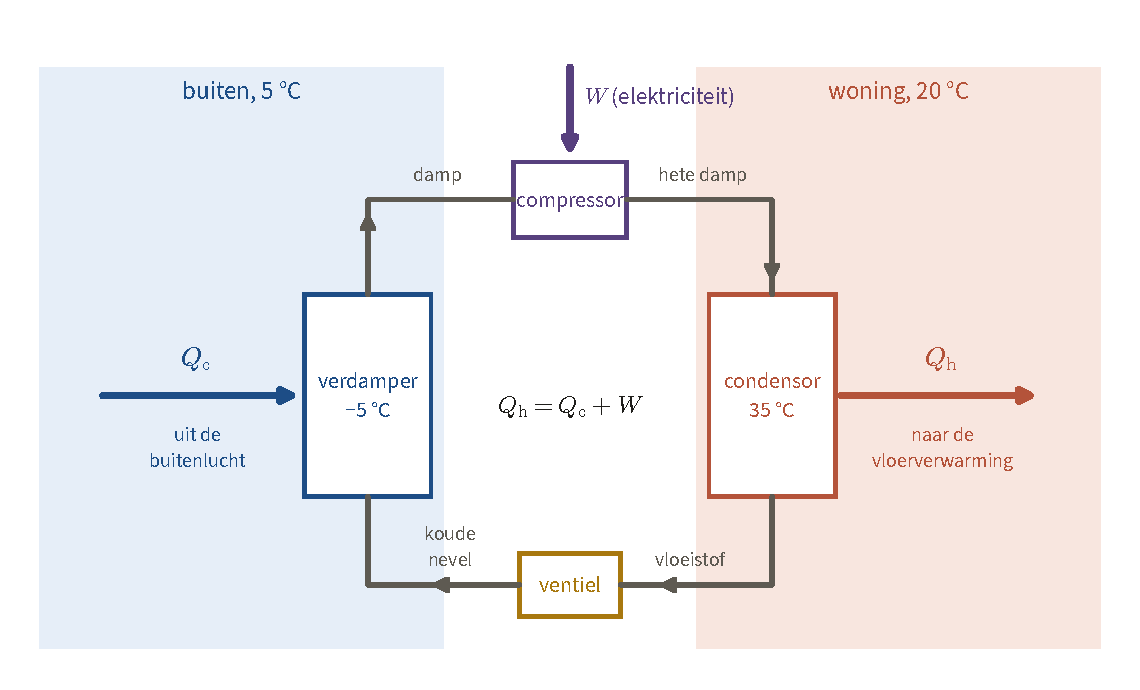
\includegraphics[width=0.85\linewidth]{Figuren/warmtepomp_schema}
    \caption{Kringloop van een lucht-waterwarmtepomp. Het koelmiddel neemt warmte $Q_\mathrm{c}$ op uit de koude buitenlucht, de compressor voegt arbeid $W$ toe, en de condensor geeft $Q_\mathrm{h} = Q_\mathrm{c} + W$ af aan de vloerverwarming.}
    \label{fig:warmtepomp}
\end{figure}

De eerste hoofdwet zegt enkel dat de energie klopt: $Q_\mathrm{h} = Q_\mathrm{c} + W$. Ze zegt niet waarom je de compressor nodig hebt. Waarom stroomt de warmte niet vanzelf van de buitenlucht naar binnen, zodat $W = 0$ volstaat? Dat soort vragen is het onderwerp van dit hoofdstuk:
\begin{itemize}
\item Waarom stroomt warmte vanzelf van warm naar koud, en nooit omgekeerd (\S\ref{sec:waarschijnlijkheid-entropie})?
\item Hoeveel elektriciteit heeft een warmtepomp minstens nodig per kilowattuur warmte, en waar hangt dat van af (\S\ref{sec:tweedehoofdwet})?
\item Is het dan beter om met een warmtepomp te verwarmen dan met een gasketel, die bijna alle energie van het gas als warmte afgeeft (\S\ref{sec:exergie})?
\item Bij welke temperatuur kookt het koelmiddel, en hoe kies je er een (\S\ref{sec:gibbs})?
\end{itemize}
Het antwoord vraagt een nieuwe grootheid, de \emph{entropie}. In hoofdstuk~\ref{ch:kwantum} zagen we dat energie over gekwantiseerde toestanden verdeeld wordt. Entropie telt op hoeveel manieren dat kan. Met de entropie volgt ook de grootheid die voor ingenieurs en chemici het belangrijkst is: de Gibbs-vrije energie, die zegt welke processen en reacties vanzelf verlopen. Net als in de vorige hoofdstukken start elke sectie met een probleem en werkt ze dat op het einde uit.

\section{Spontaniteit en de statistische oorsprong van entropie}

\begin{casus}{waarom stroomt warmte enkel van warm naar koud?}
Zet een warme kop koffie in een koude kamer en ze koelt af tot kamertemperatuur. Nooit warmt lauwe koffie zichzelf op door warmte uit de kamer te halen, hoewel de energie in beide richtingen behouden blijft. Waarom niet? Geen enkele kracht duwt de energie van warm naar koud.

\emph{Schat eerst zelf:} denk aan de energiekwanta van hoofdstuk~\ref{ch:kwantum}. Als je een handvol kwanta willekeurig verdeelt over de moleculen van twee voorwerpen, waar komen ze dan vooral terecht?
\end{casus}

Hete koffie die afkoelt, parfum dat zich door een kamer verspreidt, melk die zich mengt met koffie, een ijsblokje dat smelt in een warm drankje: het zijn heel verschillende processen, gedreven door warmteoverdracht, diffusie of een faseovergang. Toch hebben ze \'e\'en ding gemeen: ze verlopen vanzelf in \'e\'en richting, en nooit in de omgekeerde. Lauwe koffie warmt zichzelf nooit op, een mengsel ontmengt nooit vanzelf, en een glas water vormt nooit spontaan een ijsblokje op kamertemperatuur.

\subsection{Spontane processen: energie is niet het criterium}

Het ligt voor de hand om te denken dat een proces vanzelf verloopt omdat de energie daalt, zoals een bal die van een helling rolt. De eerste hoofdwet laat echter geen onderscheid toe. Stroomt \SI{1}{\kilo\joule} warmte van de koffie naar de kamer, dan verliest de koffie \SI{1}{\kilo\joule} en wint de kamer \SI{1}{\kilo\joule}. Stroomt dezelfde \SI{1}{\kilo\joule} omgekeerd, dan klopt de energiebalans evengoed. De eerste hoofdwet verbiedt geen van beide richtingen.

Twee proeven tonen dat een daling van de energie ook geen voorwaarde is.

\paragraph{De vrije expansie van Joule.} Joule plaatste in 1845 twee koperen vaten, verbonden door een kraan, in een waterbad (figuur~\ref{fig:vrije-expansie}). Het ene vat bevatte lucht onder \SI{22}{\bar}, het andere was luchtledig. Hij opende de kraan: de lucht verspreidde zich over beide vaten, en hij mat de temperatuur van het bad. Die veranderde niet. Het gas verrichtte geen arbeid (het expandeerde in het vacu\"um, tegen geen enkele tegendruk), en het wisselde geen warmte uit met het bad, dus $\Delta U = 0$. Toch verloopt de expansie vanzelf, en nooit kruipt het gas vanzelf terug in \'e\'en vat.

\begin{figure}[htb]
    \centering
    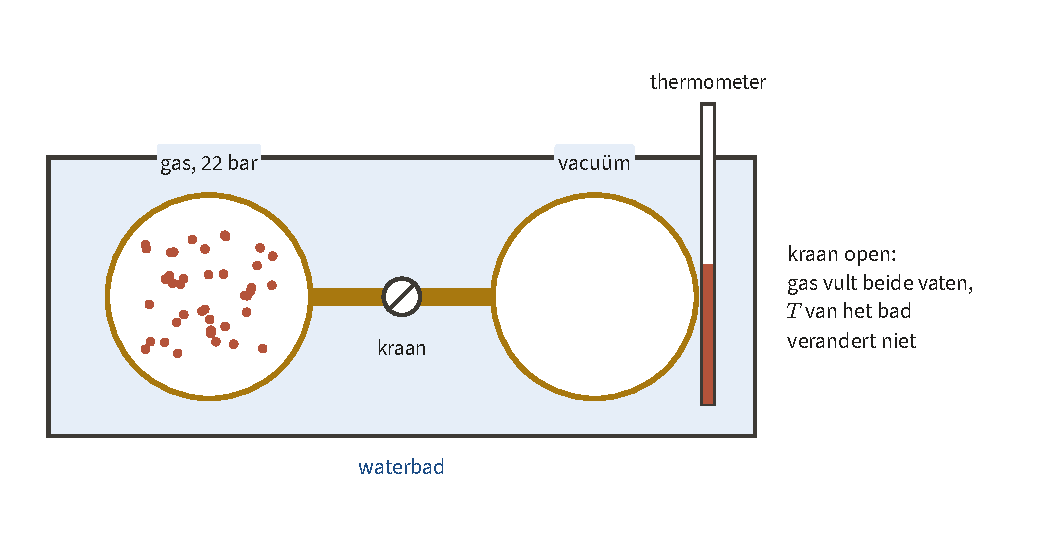
\includegraphics[width=0.8\linewidth]{Figuren/vrije_expansie}
    \caption{De vrije expansie van Joule. Na het openen van de kraan vult het gas beide vaten, terwijl de temperatuur van het bad gelijk blijft: de interne energie van het gas verandert niet, en toch verloopt het proces vanzelf in \'e\'en richting.}
    \label{fig:vrije-expansie}
\end{figure}

\paragraph{Endotherme processen die vanzelf verlopen.} Een ijsblokje in een glas limonade smelt en neemt daarbij warmte op: de enthalpie van het water stijgt. Ammoniumnitraat lost vanzelf op in water, terwijl de oplossing zo sterk afkoelt dat men er koude kompressen mee maakt. De energie van het systeem stijgt hier, en toch verloopt het proces vanzelf.

Er is dus een tweede principe nodig, naast het behoud van energie, om de richting van een proces te voorspellen. De sleutel ligt in een vaststelling die alle voorbeelden gemeen hebben: het systeem evolueert telkens naar een toestand die op moleculair niveau veel \emph{waarschijnlijker} is dan de begintoestand. Om dat te begrijpen, moeten we leren tellen.

\subsection{Microtoestanden en macrotoestanden}
\label{sec:waarschijnlijkheid-entropie}

Druk, volume, temperatuur en samenstelling beschrijven een gas als geheel. Zo'n beschrijving heet een \emph{macrotoestand}. Op moleculair niveau heeft elke molecule op elk ogenblik een eigen positie en een eigen energie. Een volledige opgave van alle posities en energie\"en heet een \emph{microtoestand}. Bij \'e\'en macrotoestand horen ontelbaar veel microtoestanden: de moleculen bewegen voortdurend en wisselen van plaats, maar de druk en temperatuur die je meet, blijven dezelfde.

Neem opnieuw het vat van Joule, maar nu met slechts vier moleculen, die we a, b, c en d noemen. Elke molecule kan zich in de linker- of de rechterhelft bevinden, onafhankelijk van de andere. Er zijn dus $2 \times 2 \times 2 \times 2 = 2^4 = 16$ microtoestanden, en omdat de moleculen voortdurend bewegen, is elk ervan even waarschijnlijk. Groeperen we ze volgens het aantal moleculen links (de macrotoestand), dan vinden we:
\begin{itemize}
\item alle vier links: 1 microtoestand (abcd);
\item drie links: 4 microtoestanden (abc, abd, acd, bcd);
\item twee links: 6 microtoestanden (ab, ac, ad, bc, bd, cd);
\item \'e\'en links: 4, en geen enkele links: 1.
\end{itemize}
De gelijkmatige verdeling is het waarschijnlijkst (6 kansen op 16), maar ``alles links'' is met 1 kans op 16 nog heel goed mogelijk (figuur~\ref{fig:microtoestanden}, links). Met duizend moleculen ligt dat helemaal anders. Het aantal microtoestanden met $n$ moleculen links is dan $1000!/(n!\,(1000-n)!)$, en de verdeling wordt een smalle piek rond de helft (figuur~\ref{fig:microtoestanden}, rechts). De kans dat alle moleculen links zitten, is $2^{-1000} \approx 10^{-301}$. Een mol gas bevat $6\times10^{23}$ moleculen: de kans op een merkbare afwijking van de gelijkmatige verdeling is daar zo klein dat je ze in de hele levensduur van het heelal nooit zou zien.

\begin{figure}[htb]
    \centering
    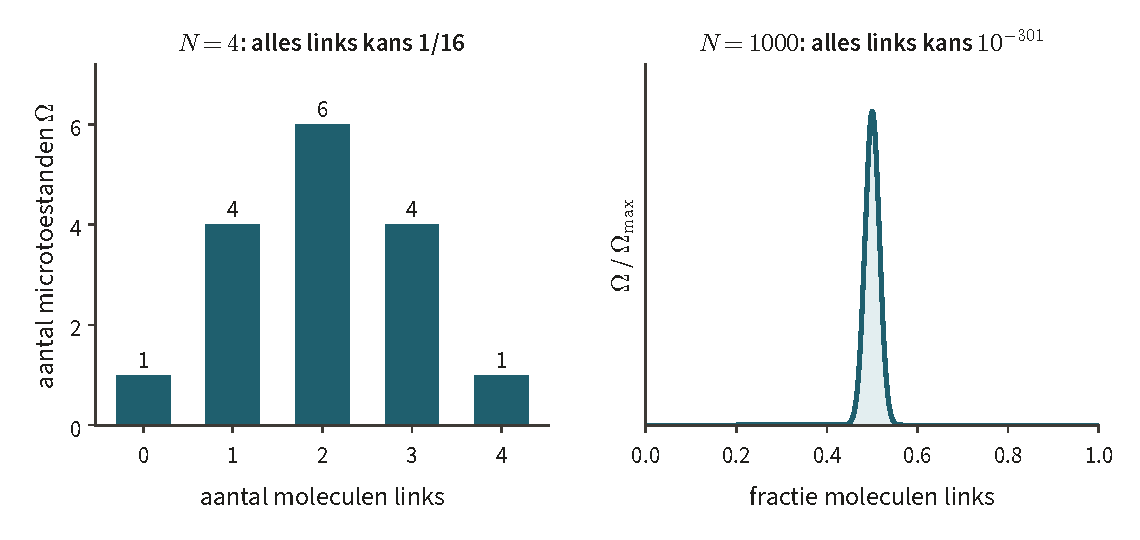
\includegraphics[width=0.9\linewidth]{Figuren/microtoestanden}
    \caption{Aantal manieren om moleculen over twee helften van een vat te verdelen. Links: bij vier moleculen is een ongelijke verdeling nog vrij waarschijnlijk. Rechts: bij duizend moleculen is de verdeling al zeer scherp rond de helft. Bij een mol gas is de kans op een merkbare afwijking praktisch nul.}
    \label{fig:microtoestanden}
\end{figure}

Dat verklaart de proef van Joule. Geen kracht duwt het gas naar het lege vat. De moleculen bewegen willekeurig, en daardoor belandt het systeem in de macrotoestand met de meeste microtoestanden, gewoon omdat die overweldigend waarschijnlijker is. De terugweg is niet verboden, maar zo onwaarschijnlijk dat hij in de praktijk nooit voorkomt.

\subsection{De formule van Boltzmann}

Ludwig Boltzmann gaf in 1877 een naam aan dit getal: hij verbond het aantal microtoestanden $\Omega$ van een macrotoestand met de \emph{entropie} $S$,
\begin{equation}
\boxed{S = k_B \ln \Omega}
\label{eq:boltzmann}
\end{equation}
met de constante van Boltzmann $k_B = R/N_A = \SI{1.381e-23}{\joule\per\kelvin}$. De formule staat op zijn grafsteen in Wenen.

\paragraph{Waarom een logaritme?} Waarom niet gewoon $S \propto \Omega$? Het antwoord volgt uit een eigenschap die we van entropie verwachten: ze moet \emph{extensief} zijn, zoals volume of massa. Voeg je twee identieke, onafhankelijke systemen samen, dan moet de entropie verdubbelen: $S_\text{tot} = S_A + S_B$. We volgen de redenering in drie stappen.
\begin{enumerate}
\item \emph{Microtoestanden vermenigvuldigen.} Voor elk van de $\Omega_A$ microtoestanden van systeem A kan systeem B zich in elk van zijn $\Omega_B$ microtoestanden bevinden. Het totale aantal combinaties is dus het \emph{product} $\Omega_\text{tot} = \Omega_A\,\Omega_B$. Zo hebben twee dobbelstenen niet $6 + 6 = 12$, maar $6 \times 6 = 36$ mogelijke uitkomsten.
\item \emph{Entropie moet optellen.} Met $S \propto \Omega$ zou het samenvoegen van twee identieke systemen de entropie niet verdubbelen maar kwadrateren. Hebben A en B elk $\Omega = 10^3$ microtoestanden, dan heeft het geheel er $10^6$: niet twee keer, maar duizend keer zoveel.
\item \emph{De logaritme zet een product om in een som.} We hebben een functie nodig met $f(\Omega_A\Omega_B) = f(\Omega_A) + f(\Omega_B)$. Dat is precies de eigenschap van de logaritme, en ze is de enige functie die eraan voldoet. In het voorbeeld: $\ln(10^6) = 6\ln 10 = 2 \times (3\ln 10) = 2\ln(10^3)$. De logaritme van het geheel is wel precies het dubbele van die van elk deel.
\end{enumerate}
De logaritme blijft bovendien stijgen met $\Omega$: een macrotoestand met meer microtoestanden heeft een hogere entropie. De constante $k_B$ is enkel een schaalfactor, zo gekozen dat de statistische entropie dezelfde waarde en eenheid (\si{\joule\per\kelvin}) heeft als de klassieke entropie die Clausius al eerder uit warmtemetingen had afgeleid (\S\ref{sec:tweedehoofdwet}).

Entropie is dus een maat voor het aantal manieren waarop een macrotoestand kan worden gerealiseerd. Mengen, warmte die van warm naar koud stroomt, een gas dat expandeert: telkens gaat het systeem naar een toestand met meer microtoestanden, dus met een hogere entropie. We maken dat nu kwantitatief voor twee situaties die je als ingenieur steeds tegenkomt: een gas dat uitzet, en twee stoffen die mengen.

\subsubsection{Entropieverandering bij isotherme expansie}

We berekenen hoeveel de entropie stijgt wanneer een ideaal gas bij constante temperatuur uitzet van $V_1$ naar $V_2$, zoals in de proef van Joule.
\begin{enumerate}
\item \emph{Tel de plaatsen voor \'e\'en molecule.} Verdeel het volume, louter als rekenhulp, in kleine cellen met volume $v_0$. Een molecule heeft dan $V/v_0$ mogelijke plaatsen (figuur~\ref{fig:expansie-cellen}).
\item \emph{Tel de schikkingen voor $N$ moleculen.} In een ideaal gas be\"invloeden de moleculen elkaar niet, dus elke molecule kiest onafhankelijk. Net als bij de dobbelstenen vermenigvuldigen de mogelijkheden: $\Omega \propto (V/v_0)^N$.
\item \emph{Neem de verhouding.} Bij constante temperatuur verandert de verdeling van de energie niet, enkel het aantal plaatsen. Dus $\Omega_2/\Omega_1 = (V_2/V_1)^N$; de willekeurige celgrootte $v_0$ valt weg.
\item \emph{Pas Boltzmann toe.} $\Delta S = k_B\ln\Omega_2 - k_B\ln\Omega_1 = k_B\ln(\Omega_2/\Omega_1) = Nk_B\ln(V_2/V_1)$. Met $N = nN_A$ en $k_BN_A = R$:
\end{enumerate}
\begin{equation}
\boxed{\Delta S = nR\ln\frac{V_2}{V_1} \qquad \text{(isotherme expansie van een ideaal gas)}}
\label{eq:dS-expansie}
\end{equation}

\begin{figure}[htb]
    \centering
    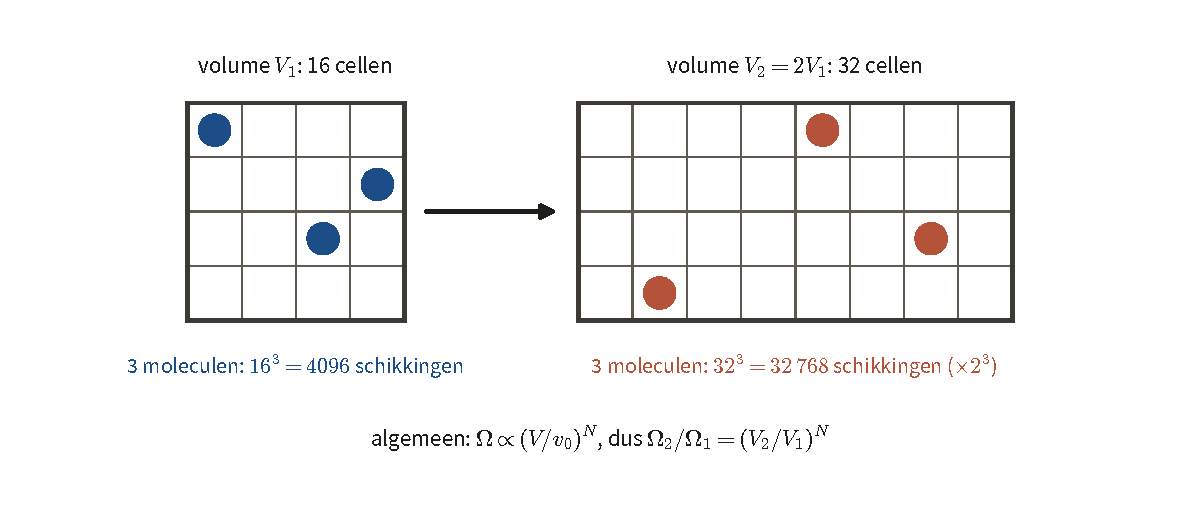
\includegraphics[width=0.85\linewidth]{Figuren/expansie_cellen}
    \caption{Verdubbelt het volume, dan verdubbelt het aantal plaatsen voor elke molecule. Voor drie moleculen stijgt het aantal schikkingen met een factor $2^3 = 8$, voor $N$ moleculen met $2^N$.}
    \label{fig:expansie-cellen}
\end{figure}

\begin{voorbeeld}{Entropie bij een volumeverdubbeling}
\SI{1}{\mole} ideaal gas zet bij constante temperatuur uit van \SI{10}{\litre} naar \SI{20}{\litre}:
\[
\Delta S = nR\ln\frac{V_2}{V_1} = (1)(8.314)\ln 2 = \SI{5.76}{\joule\per\kelvin}.
\]
Een klein getal, maar achter die \SI{5.76}{\joule\per\kelvin} zit een gigantische toename van het aantal microtoestanden: $\Omega_2/\Omega_1 = 2^{6\times10^{23}}$. De logaritme maakt er een hanteerbaar getal van.
\end{voorbeeld}

Merk op dat in deze afleiding nergens warmte of arbeid voorkomt: het resultaat volgt enkel uit tellen. In \S\ref{sec:tweedehoofdwet} zullen we dezelfde formule terugvinden langs een heel andere weg, uit een warmtemeting.

\subsubsection{Entropieverandering bij mengen}

Bij mengen gaat het niet om meer plaatsen, maar om meer manieren om twee soorten moleculen over dezelfde plaatsen te verdelen. Verdeel $N_A$ moleculen A en $N_B$ moleculen B over $N = N_A + N_B$ plaatsen van een rooster.
\begin{enumerate}
\item \emph{Tel de schikkingen.} Zolang A en B gescheiden zijn, elk in hun eigen deel, is er voor het patroon maar \'e\'en schikking: $\Omega = 1$. Na het mengen kies je welke $N_A$ van de $N$ plaatsen door A worden ingenomen; de rest is voor B. Dat kan op
\[
\Omega = \frac{N!}{N_A!\,N_B!}
\]
manieren. Voor een klein rooster met 8 moleculen A en 8 moleculen B is dat al $16!/(8!\,8!) = 12\,870$ (figuur~\ref{fig:menging-rooster}).
\item \emph{Vereenvoudig met Stirling.} Voor grote getallen geldt $\ln x! \approx x\ln x - x$ (de benadering van Stirling, al op een procent nauwkeurig vanaf $x = 100$). Zo wordt
\[
\ln\Omega \approx N\ln N - N_A\ln N_A - N_B\ln N_B ,
\]
waarbij de termen $-N + N_A + N_B$ wegvallen.
\item \emph{Schrijf in molfracties.} Splits $N\ln N = N_A\ln N + N_B\ln N$ en groepeer: $\ln\Omega = -N_A\ln(N_A/N) - N_B\ln(N_B/N) = -N_A\ln x_A - N_B\ln x_B$.
\item \emph{Pas Boltzmann toe en reken per mol.} Met $\Delta S = k_B\ln\Omega$, $N_i = n_iN_A$ en $k_BN_A = R$ volgt, gedeeld door het totale aantal mol:
\end{enumerate}
\begin{equation}
\boxed{\Delta S_{\text{meng}} = -R\bigl(x_A\ln x_A + x_B\ln x_B\bigr) > 0 .}
\label{eq:mengentropie}
\end{equation}
Omdat elke molfractie kleiner is dan 1, is elke $\ln x_i$ negatief, en is de mengentropie altijd positief: mengen verhoogt altijd het aantal microtoestanden. Ze is maximaal bij een 50/50-mengsel.

\begin{figure}[htb]
    \centering
    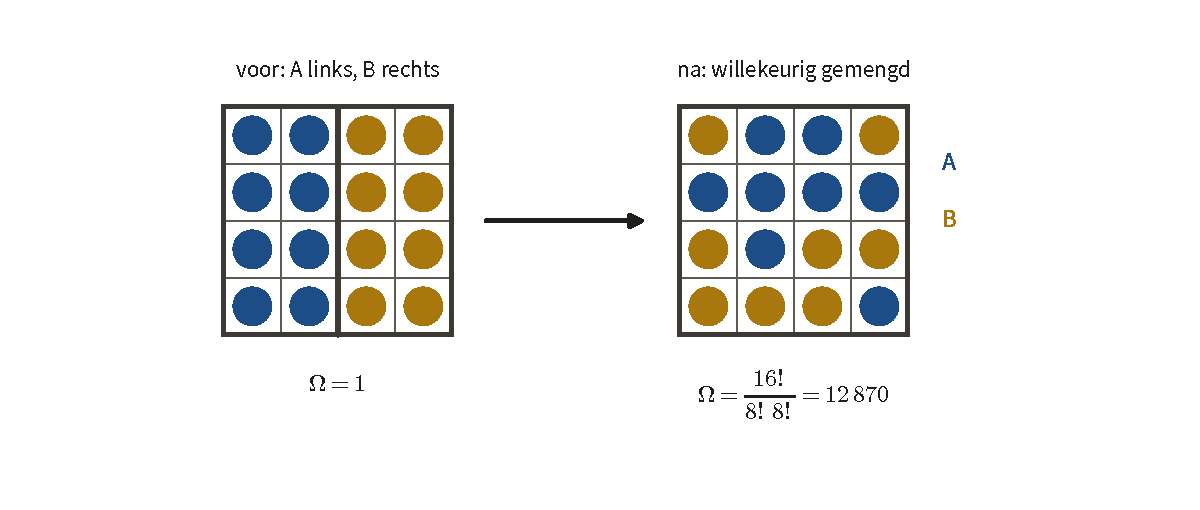
\includegraphics[width=0.85\linewidth]{Figuren/menging_rooster}
    \caption{Mengen op een rooster. Gescheiden is er \'e\'en schikking van A en B; gemengd zijn er voor dit kleine rooster al 12\,870. Bij een mol moleculen loopt dat op tot een getal met $10^{23}$ cijfers.}
    \label{fig:menging-rooster}
\end{figure}

\begin{voorbeeld}{Mengentropie van lucht, en de minimale arbeid om ze te scheiden}
Voor een 50/50-mengsel van \ce{N2} en \ce{O2} is $\Delta S_\text{meng} = -R(0.5\ln 0.5 + 0.5\ln 0.5) = R\ln 2 = \SI{5.76}{\joule\per\mole\per\kelvin}$: precies dezelfde waarde als bij de volumeverdubbeling. Dat is geen toeval: na het mengen heeft elke molecule twee keer zoveel ruimte, net als bij de expansie.

Echte lucht bevat \SI{79}{\percent} \ce{N2} en \SI{21}{\percent} \ce{O2} (argon rekenen we bij de stikstof):
\[
\Delta S_\text{meng} = -R(0.79\ln 0.79 + 0.21\ln 0.21) = (8.314)(0.186 + 0.328) = \SI{4.27}{\joule\per\mole\per\kelvin}.
\]
Omgekeerd verloopt het scheiden van lucht nooit vanzelf: het kost arbeid. Hoeveel minstens, zie je in oefening~\ref{oef:meng-scheiden}: het komt neer op $T\Delta S_\text{meng} \approx (298)(4.27) = \SI{1.3}{\kilo\joule}$ per mol lucht. Een echte luchtscheidingsinstallatie, die de stikstof voor de ammoniakfabriek levert, verbruikt vijf tot tien keer meer. Waar die extra arbeid verloren gaat, is een vraag voor de scheidingstechnologie.
\end{voorbeeld}

\begin{figure}[htb]
    \centering
    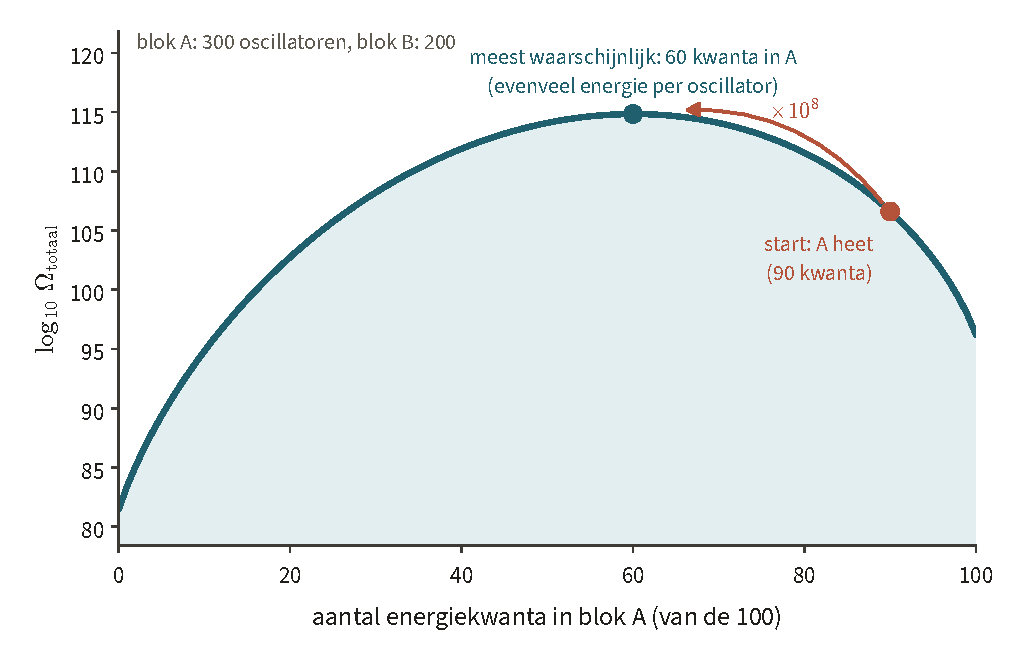
\includegraphics[width=0.75\linewidth]{Figuren/twee_blokken}
    \caption{Twee blokken in thermisch contact delen 100 energiekwanta. Blok A heeft 300 trillende atomen (oscillatoren), blok B 200. Voor elke verdeling is $\Omega_\text{totaal} = \Omega_A\Omega_B$ uitgezet (logaritmische schaal). Start A met 90 kwanta (heet), dan zijn er $10^8$ keer meer microtoestanden wanneer de energie zich herverdeelt tot evenveel energie per oscillator.}
    \label{fig:twee-blokken}
\end{figure}

\begin{casusuitgewerkt}{waarom stroomt warmte enkel van warm naar koud?}
Bekijk twee kleine blokken die energiekwanta uitwisselen (figuur~\ref{fig:twee-blokken}). Een blok met $N$ trillende atomen en $q$ kwanta kan die kwanta op
\[
\Omega(N,q) = \frac{(q+N-1)!}{q!\,(N-1)!}
\]
manieren verdelen (het aantal manieren om $q$ gelijke ballen over $N$ dozen te verdelen). Samen is $\Omega_\text{totaal} = \Omega_A\Omega_B$.

\emph{Stap 1: de begintoestand.} Blok A (300 atomen) heeft 90 van de 100 kwanta, blok B (200 atomen) slechts 10. Per atoom heeft A dus zes keer meer energie: A is heet, B is koud. Er zijn $10^{106.6}$ microtoestanden.

\emph{Stap 2: de evenwichtstoestand.} Het maximum ligt bij 60 kwanta in A en 40 in B: evenveel energie per atoom, dus dezelfde temperatuur. Daar zijn er $10^{114.8}$ microtoestanden, $10^8$ keer meer.

\emph{Stap 3: het besluit.} Botsingen verdelen de kwanta voortdurend opnieuw, zonder voorkeur. Het systeem belandt daardoor bijna zeker in de verdeling met de meeste microtoestanden. Warmte stroomt van warm naar koud, niet omdat een kracht haar duwt, maar omdat er overweldigend veel meer manieren zijn om de energie gelijkmatig te verdelen. Met 100 kwanta is de terugweg naar 90 kwanta in A al honderd miljoen keer minder waarschijnlijk; voor een kop koffie met $10^{25}$ moleculen is hij onmogelijk. Hetzelfde geldt voor de buitenlucht en de woning: de warmte gaat vanzelf naar buiten, nooit naar binnen.

\emph{Volgende vraag.} Een warmtepomp dwingt de warmte toch de ``verkeerde'' kant op. Hoe reken je uit hoeveel arbeid dat minstens kost, zonder microtoestanden te tellen?
\end{casusuitgewerkt}

\section{De tweede hoofdwet en de klassieke formulering van entropie}
\label{sec:tweedehoofdwet}

\begin{casus}{hoeveel stroom vraagt een warmtepomp?}
Een warmtepomp levert \SI{10}{\kilo\watt} warmte aan een vloerverwarming van \SI{35}{\celsius}, terwijl het buiten \SI{5}{\celsius} is. Hoeveel elektrisch vermogen heeft de compressor daar minstens voor nodig? En hoeveel als de woning radiatoren van \SI{55}{\celsius} heeft?

\emph{Schat eerst zelf:} moet de compressor evenveel arbeid leveren als de warmte die binnenkomt, meer, of veel minder? Waarom zou de afgiftetemperatuur ertoe doen?
\end{casus}


\subsection{De tweede hoofdwet van de thermodynamica}

De tweede hoofdwet werd niet ontdekt door moleculen te tellen, maar door naar stoommachines te kijken. Sadi Carnot vroeg zich in 1824 af hoeveel arbeid een stoommachine maximaal uit een hoeveelheid steenkool kan halen. Hij en later Kelvin en Clausius stelden vast dat elke warmtemachine een deel van de opgenomen warmte moet afgeven aan een koudere omgeving, hoe goed ze ook gebouwd is. Uit die ervaring formuleerden ze twee gelijkwaardige uitspraken:
\begin{itemize}
\item \emph{Kelvin (1851):} geen enkele machine die een kringloop doorloopt, kan warmte uit \'e\'en reservoir volledig omzetten in arbeid.
\item \emph{Clausius (1850):} warmte stroomt nooit vanzelf van een koud naar een warm lichaam.
\end{itemize}
Beide uitspraken zijn veralgemeningen van ontelbare waarnemingen; niemand heeft ooit een tegenvoorbeeld gevonden. Boltzmann toonde later waarom: ze zijn het macroscopische gevolg van het tellen van microtoestanden. Een ge\"isoleerd systeem gaat naar de macrotoestand met de meeste microtoestanden, dus met de hoogste entropie. Dat geeft de algemeenste vorm van de wet.

\begin{definitie}{Tweede hoofdwet van de thermodynamica}
De totale entropie van een ge\"isoleerd systeem neemt bij elk spontaan proces toe:
\begin{equation}
\Delta S_{\text{univ}} \geq 0,
\end{equation}
met het gelijkheidsteken enkel voor een reversibel proces.
\end{definitie}

Het woord ``universum'' klinkt groots, maar betekent hier gewoon: het systeem samen met alles waarmee het energie uitwisselt, zodat het geheel ge\"isoleerd is. Voor een kop koffie op tafel is dat de koffie plus de kamer. De eerste hoofdwet gaat over de \emph{hoeveelheid} energie, de tweede over de \emph{richting} waarin processen lopen.

\subsection{De Clausius-definitie: entropie uit warmte}

Microtoestanden tellen lukt voor een ideaal gas of een eenvoudig model, maar niet voor de stoom in een turbine of het koelmiddel in een warmtepomp. Voor de ingenieur is een tweede, gelijkwaardige definitie veel bruikbaarder. Clausius vond al in 1865, nog v\'o\'or Boltzmann, dat je de entropieverandering kan \emph{meten} via de warmte die een systeem reversibel opneemt:
\begin{equation}
\boxed{\dd S = \frac{\delta Q_{\text{rev}}}{T}}
\label{eq:clausius}
\end{equation}

\paragraph{Waarom warmte gedeeld door temperatuur?} Twee vaststellingen maken die vorm aannemelijk.
\begin{enumerate}
\item \emph{Warmte verhoogt het aantal microtoestanden.} Voeg je energie toe aan een systeem, dan zijn er meer kwanta om over de moleculen te verdelen, en dus meer manieren om dat te doen. Arbeid die reversibel een zuiger verplaatst, doet dat niet: ze verandert enkel het volume of de positie, op een ordelijke manier. Daarom staat in de teller warmte, geen arbeid.
\item \emph{Dezelfde warmte doet meer bij lage temperatuur.} Een koud systeem heeft weinig energie, verdeeld over weinig kwanta. Wat extra energie zet daar relatief veel nieuwe verdelingen open. Een warm systeem bevat al veel energie; dezelfde portie verandert er relatief weinig. Vergelijk het met niezen: in een stille bibliotheek valt het op, op een drukke markt niemand. Daarom staat $T$ in de noemer.
\end{enumerate}

\paragraph{Toets 1: warmte van warm naar koud.} Laat \SI{1000}{\joule} warmte stromen van koffie van \SI{80}{\celsius} naar een kamer van \SI{20}{\celsius} (figuur~\ref{fig:warmtestroom-entropie}). Beide zijn zo groot dat hun temperatuur nauwelijks verandert. De koffie verliest $1000/353 = \SI{2.83}{\joule\per\kelvin}$ entropie, de kamer wint $1000/293 = \SI{3.41}{\joule\per\kelvin}$. Samen is $\Delta S_\text{univ} = \SI{+0.58}{\joule\per\kelvin}$: het proces verloopt vanzelf. De omgekeerde richting zou $\SI{-0.58}{\joule\per\kelvin}$ geven, en is dus onmogelijk. De definitie van Clausius levert zo precies de uitspraak van Clausius op, en de tweeblokkenproef van de casus in getallen.

\begin{figure}[htb]
    \centering
    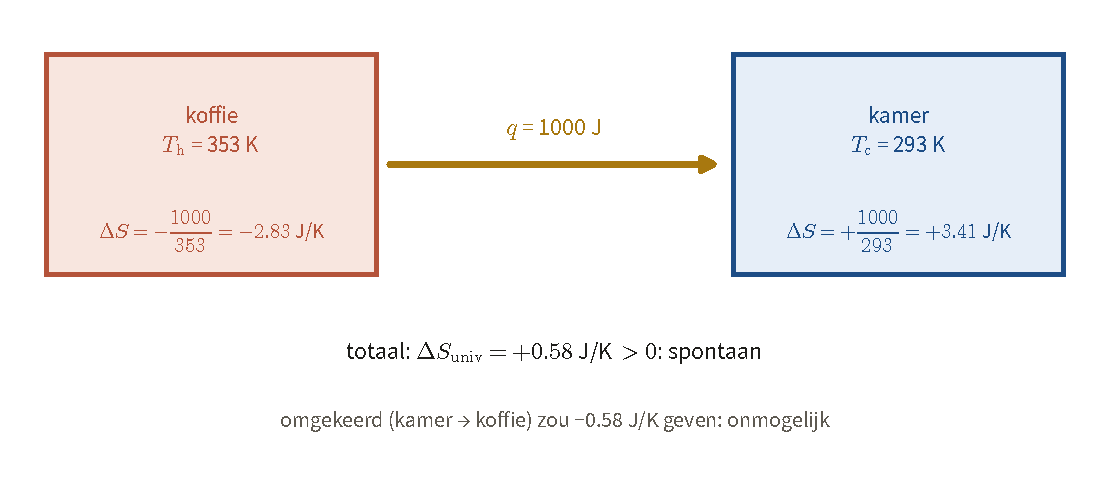
\includegraphics[width=0.8\linewidth]{Figuren/warmtestroom_entropie}
    \caption{Entropiebalans voor \SI{1}{\kilo\joule} warmte die van hete koffie naar de kamer stroomt. Dezelfde warmte verhoogt de entropie van de koude kamer meer dan ze die van de warme koffie verlaagt.}
    \label{fig:warmtestroom-entropie}
\end{figure}

\paragraph{Toets 2: dezelfde formule als Boltzmann.} Laat \SI{1}{\mole} ideaal gas reversibel en isotherm uitzetten van $V_1$ naar $V_2$, door een zuiger heel langzaam te laten wijken terwijl het gas in contact staat met een warmtebad. In hoofdstuk~\ref{ch:energie} zagen we twee dingen: bij constante temperatuur is $\Delta U = 0$ voor een ideaal gas, en de arbeid is $W = -nRT\ln(V_2/V_1)$. Uit de eerste hoofdwet volgt $Q_\text{rev} = -W = nRT\ln(V_2/V_1)$, en met Clausius
\[
\Delta S = \frac{Q_\text{rev}}{T} = nR\ln\frac{V_2}{V_1}.
\]
Dat is exact vergelijking~\eqref{eq:dS-expansie}, die we uit het tellen van cellen haalden. Twee volledig verschillende redeneringen, de ene met warmte en temperatuur, de andere met microtoestanden, leveren dezelfde entropie. Dat is de sterkste aanwijzing dat beide over dezelfde grootheid gaan.

\paragraph{Toets 3: een irreversibel proces.} Nu de vrije expansie van Joule, tussen dezelfde begin- en eindtoestand. Het gas neemt geen warmte op ($Q = 0$). Toch is de entropie gestegen met $nR\ln(V_2/V_1)$, want entropie is een toestandsfunctie: ze hangt enkel af van begin- en eindtoestand, en die zijn dezelfde als bij de reversibele expansie. Bij een irreversibel proces is de entropietoename dus \emph{groter} dan $Q/T$. Dat geeft de \emph{ongelijkheid van Clausius}:
\begin{equation}
\dd S \geq \frac{\delta Q}{T},
\end{equation}
met het gelijkheidsteken enkel voor een reversibel proces. Het verschil is de entropie die door het proces zelf wordt \emph{geproduceerd}: door wrijving, door warmte die over een eindig temperatuurverschil stroomt, door menging, of zoals hier door een gas dat ongeremd uitzet.

Uit toets 3 volgt ook de praktische werkwijze om een entropieverandering te berekenen: omdat $S$ een toestandsfunctie is, kies je altijd een \emph{denkbeeldige reversibele weg} tussen dezelfde begin- en eindtoestand, ook als het echte proces irreversibel was, en berekent daarlangs $\int\delta Q_\text{rev}/T$. Twee zulke wegen komen in de praktijk telkens terug: een faseovergang en het opwarmen van een stof.

\subsubsection{Entropie bij faseovergangen}
\label{sec:entropie-faseovergangen}

In hoofdstuk~\ref{ch:energie} (figuur~\ref{fig:opwarmcurve}) zagen we dat de temperatuur tijdens het smelten of koken constant blijft: alle toegevoerde warmte gaat naar het verbreken van intermoleculaire bindingen, niet naar snellere beweging. Bij constante druk is die warmte de faseovergangsenthalpie, en ze wordt bij \'e\'en vaste temperatuur opgenomen. In vergelijking~\eqref{eq:clausius} is $T$ dan constant, en de integratie is onmiddellijk:
\begin{equation}
\Delta S_{\text{trans}} = \frac{\Delta H_{\text{trans}}}{T_{\text{trans}}} .
\label{eq:entropie_fase}
\end{equation}
Voor water vind je
\[
\Delta S_\text{fus} = \frac{6010}{273.15} = \SI{22.0}{\joule\per\mole\per\kelvin},
\qquad
\Delta S_\text{vap} = \frac{40\,700}{373.15} = \SI{109}{\joule\per\mole\per\kelvin}.
\]
De verdampingsentropie is vijf keer groter dan de smeltentropie. Moleculair is dat logisch: bij smelten blijven de moleculen dicht op elkaar, ze krijgen enkel vrijheid om langs elkaar te bewegen en te draaien. Bij verdampen neemt elke molecule ongeveer 1700 keer meer volume in, en met $nR\ln(V_2/V_1)$ is dat alleen al $R\ln 1700 = \SI{62}{\joule\per\mole\per\kelvin}$. Vergelijking~\eqref{eq:entropie_fase} is ook de basis van de vergelijking van Clapeyron (hoofdstuk~\ref{ch:niet-reagerend}).

\subsubsection{Entropieverandering bij opwarming}
\label{sec:entropie-opwarming}

Warm je een stof op zonder dat ze van fase verandert, dan stijgt de temperatuur tijdens het opnemen van de warmte. We leiden de entropieverandering af in drie stappen.
\begin{enumerate}
\item \emph{Een klein stapje.} Bij constante druk is de warmte om de temperatuur met $\dd T$ te verhogen $\delta Q_\text{rev} = nC_p\,\dd T$ (hoofdstuk~\ref{ch:energie}). Langzaam opwarmen, telkens met een bad dat net iets warmer is, maakt dat reversibel.
\item \emph{Deel door $T$.} Volgens Clausius is $\dd S = nC_p\,\dd T/T$.
\item \emph{Tel alle stapjes op.} Integreer van $T_1$ tot $T_2$. Voor constante $C_p$:
\end{enumerate}
\begin{equation}
\boxed{\Delta S = \int_{T_1}^{T_2}\frac{nC_p}{T}\,\dd T = nC_p\ln\frac{T_2}{T_1}}
\qquad\text{(constante $C_p$)}.
\label{eq:dS-opwarming}
\end{equation}
Waar de enthalpie lineair stijgt met de temperatuur, $\Delta H = nC_p\,\Delta T$, stijgt de entropie logaritmisch: elke volgende joule wordt bij een hogere temperatuur toegevoegd en levert dus minder entropie op. Bij constant volume geldt dezelfde formule met $C_V$. Over een traject met faseovergangen tel je de stukken gewoon op: opwarmen met vergelijking~\eqref{eq:dS-opwarming}, faseovergangen met vergelijking~\eqref{eq:entropie_fase} (figuur~\ref{fig:entropie-opwarming}).

\begin{figure}[htb]
    \centering
    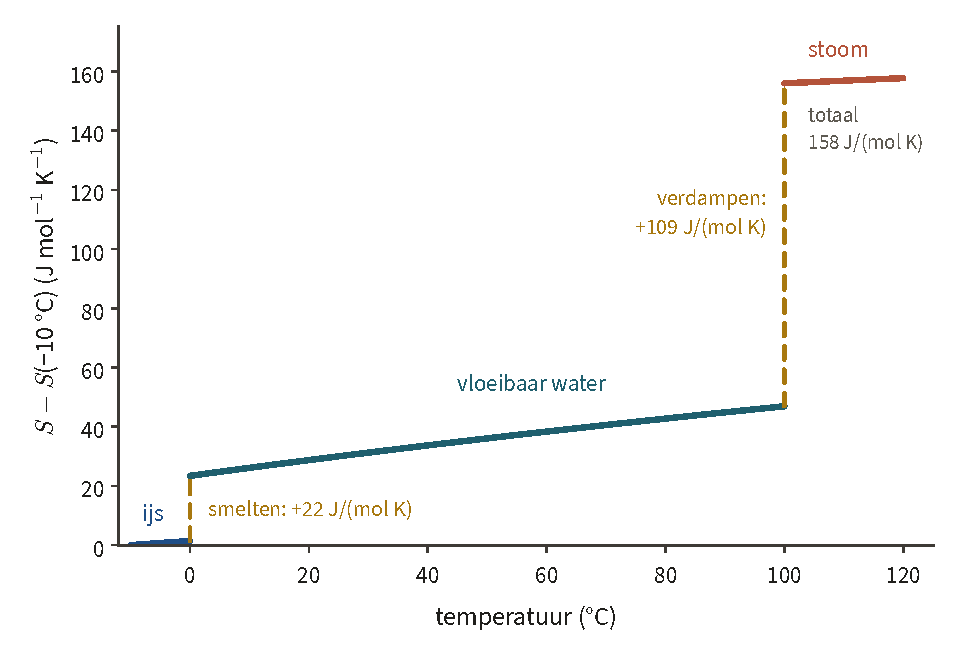
\includegraphics[width=0.75\linewidth]{Figuren/entropie_opwarming_water}
    \caption{Entropie van \SI{1}{\mole} water bij \SI{1}{\bar}, van ijs bij \SI{-10}{\celsius} tot stoom bij \SI{120}{\celsius}. Elke opwarmfase volgt vergelijking~\eqref{eq:dS-opwarming}; bij smelten en verdampen springt de entropie verticaal omhoog. De sprong bij verdampen is vijf keer groter dan die bij smelten: een gas heeft veel meer microtoestanden dan een vloeistof.}
    \label{fig:entropie-opwarming}
\end{figure}

\begin{voorbeeld}{Van ijs bij $-10\,^\circ$C tot stoom bij $120\,^\circ$C}
We berekenen de entropieverandering wanneer \SI{1}{\mole} water bij \SI{1}{\bar} wordt opgewarmd van ijs bij \SI{263.15}{\kelvin} tot stoom bij \SI{393.15}{\kelvin}. Gegevens: $C_p$ = 38.0 (ijs), 75.3 (water) en 33.6 (stoom) \si{\joule\per\mole\per\kelvin}; $\Delta H_\text{fus} = \SI{6.01}{\kilo\joule\per\mole}$ bij \SI{273.15}{\kelvin}; $\Delta H_\text{vap} = \SI{40.7}{\kilo\joule\per\mole}$ bij \SI{373.15}{\kelvin}. Het traject bestaat uit vijf stappen.

\textbf{1. IJs opwarmen} van 263.15 naar \SI{273.15}{\kelvin}: $\Delta S_1 = 38.0\ln(273.15/263.15) = (38.0)(0.0373) = \SI{1.42}{\joule\per\mole\per\kelvin}$.

\textbf{2. Smelten} bij \SI{273.15}{\kelvin}: $\Delta S_2 = 6010/273.15 = \SI{22.00}{\joule\per\mole\per\kelvin}$.

\textbf{3. Water opwarmen} van 273.15 naar \SI{373.15}{\kelvin}: $\Delta S_3 = 75.3\ln(373.15/273.15) = (75.3)(0.3120) = \SI{23.49}{\joule\per\mole\per\kelvin}$.

\textbf{4. Verdampen} bij \SI{373.15}{\kelvin}: $\Delta S_4 = 40\,700/373.15 = \SI{109.07}{\joule\per\mole\per\kelvin}$.

\textbf{5. Stoom opwarmen} van 373.15 naar \SI{393.15}{\kelvin}: $\Delta S_5 = 33.6\ln(393.15/373.15) = (33.6)(0.0522) = \SI{1.75}{\joule\per\mole\per\kelvin}$.

\textbf{Totaal:} $\Delta S = 1.42 + 22.00 + 23.49 + 109.07 + 1.75 = \SI{157.7}{\joule\per\mole\per\kelvin}$.

Verdampen alleen levert bijna 70\,\% van het totaal. Het opwarmen van vloeibaar water over \SI{100}{\kelvin} kost veel meer warmte (\SI{7.5}{\kilo\joule}) dan het smelten (\SI{6.0}{\kilo\joule}), maar levert ongeveer evenveel entropie, omdat die warmte bij hogere temperatuur wordt opgenomen.
\end{voorbeeld}

\subsection{Lokale entropieafname}

De tweede hoofdwet gaat over het \emph{totaal}. De entropie van het systeem zelf mag best dalen, als de omgeving meer wint. Water dat bevriest, een eiwit dat zich opvouwt, een koelkast die haar binnenkant afkoelt: telkens wordt het systeem geordender. Om na te gaan of zo'n proces toch vanzelf kan verlopen, moet je ook de omgeving meerekenen. Dat gaat in drie stappen.
\begin{enumerate}
\item \emph{Het systeem.} De entropieverandering van het systeem bereken je zoals hierboven, of voor een reactie met getabelleerde standaardentropie\"en (\S\ref{sec:derde-hoofdwet}).
\item \emph{De omgeving.} De omgeving is groot (de lucht, het koelwater, het labo) en blijft op een vaste temperatuur $T$. Voor zo'n reservoir is elke warmte-uitwisseling reversibel, dus is haar entropieverandering gewoon de ontvangen warmte gedeeld door $T$. Bij constante druk geeft het systeem $-\Delta H$ aan warmte af, dus
\[
\Delta S_\text{omg} = -\frac{\Delta H}{T}.
\]
Een exotherme reactie ($\Delta H < 0$) verhoogt de entropie van de omgeving.
\item \emph{De som.} Het proces verloopt vanzelf als $\Delta S_\text{univ} = \Delta S + \Delta S_\text{omg} > 0$.
\end{enumerate}

\begin{voorbeeld}{De vorming van water}
Waterstof en zuurstof reageren explosief tot water: \ce{2 H2(g) + O2(g) -> 2 H2O(l)} bij \SI{298}{\kelvin} en \SI{1}{\bar}. Gegevens: $S_m^\circ$ = 130.7 (\ce{H2}), 205.2 (\ce{O2}) en 70.0 (\ce{H2O(l)}) \si{\joule\per\mole\per\kelvin}; $\Delta_fH^\circ(\ce{H2O(l)}) = \SI{-285.8}{\kilo\joule\per\mole}$.

\textbf{1. Het systeem.} 
\[
\Delta_r S^\circ = 2(70.0) - [2(130.7) + 205.2] = \SI{-326.6}{\joule\per\kelvin}.
\]
Sterk negatief: drie mol gas, met veel bewegingsvrijheid, worden twee mol vloeistof. Op basis van het systeem alleen zou je besluiten dat de reactie niet vanzelf kan verlopen, terwijl ze een van de heftigste reacties is die we kennen.

\textbf{2. De omgeving.} De reactie is sterk exotherm, $\Delta_r H^\circ = 2(-285.8) = \SI{-571.6}{\kilo\joule}$. Die warmte komt in de omgeving terecht:
\[
\Delta S_\text{omg} = -\frac{\Delta_r H^\circ}{T} = \frac{571\,600}{298} = \SI{+1917}{\joule\per\kelvin}.
\]

\textbf{3. De som.} $\Delta S_\text{univ} = -326.6 + 1917 = \SI{+1590}{\joule\per\kelvin} > 0$ (figuur~\ref{fig:entropiebalans-water}). De orde die in het systeem ontstaat, wordt ruimschoots betaald door de warmte die de omgeving opwarmt. Bij een exotherme reactie wint de omgeving bijna altijd, zeker bij lage temperatuur, waar $-\Delta H/T$ groot is.
\end{voorbeeld}

\begin{figure}[htb]
    \centering
    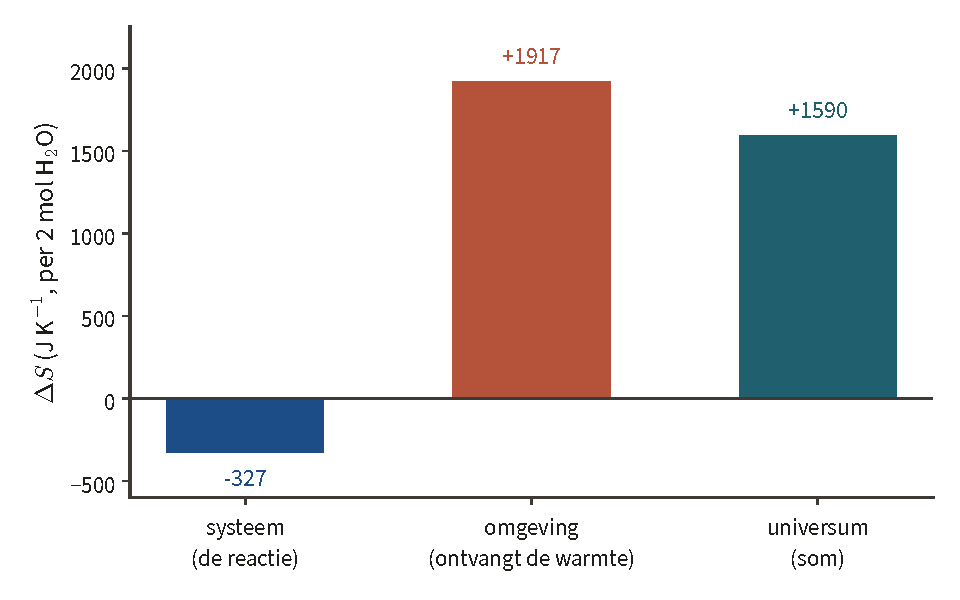
\includegraphics[width=0.65\linewidth]{Figuren/entropiebalans_water}
    \caption{Entropiebalans voor de vorming van 2 mol vloeibaar water bij \SI{298}{\kelvin}. De entropie van het systeem daalt, maar die van de omgeving stijgt bijna zes keer meer door de vrijgekomen warmte.}
    \label{fig:entropiebalans-water}
\end{figure}

Hetzelfde principe verklaart een koelkast of warmtepomp: ze maakt een ruimte kouder (lagere entropie), maar verbruikt daarvoor arbeid en dumpt meer warmte, met meer entropie, in de keuken. Hoeveel arbeid minstens nodig is, volgt uit precies zo'n balans.

\subsection{Warmtemachines, koelmachines en warmtepompen}
\label{sec:carnot}

Met de entropie kunnen we nu de grens berekenen voor elk toestel dat warmte en arbeid omzet. Bekijk een warmtepomp die in stationaire werking per cyclus warmte $Q_\mathrm{c}$ opneemt bij de lage temperatuur $T_\mathrm{c}$, arbeid $W$ ontvangt en warmte $Q_\mathrm{h} = Q_\mathrm{c} + W$ afgeeft bij de hoge temperatuur $T_\mathrm{h}$ (figuur~\ref{fig:warmtepomp}). Het koelmiddel doorloopt een kringloop en keert telkens terug naar dezelfde toestand: zijn entropie verandert over een cyclus niet. Enkel de twee warmtereservoirs veranderen van entropie: de buitenlucht verliest $Q_\mathrm{c}/T_\mathrm{c}$, de woning wint $Q_\mathrm{h}/T_\mathrm{h}$. De tweede hoofdwet eist
\[
\Delta S_\text{univ} = \frac{Q_\mathrm{h}}{T_\mathrm{h}} - \frac{Q_\mathrm{c}}{T_\mathrm{c}} \geq 0
\quad\Longrightarrow\quad
\frac{Q_\mathrm{c}}{Q_\mathrm{h}} \leq \frac{T_\mathrm{c}}{T_\mathrm{h}}.
\]
De woning moet dus minstens zoveel entropie ontvangen als de buitenlucht verliest. Omdat $T_\mathrm{h} > T_\mathrm{c}$, kan dat enkel als $Q_\mathrm{h}$ groter is dan $Q_\mathrm{c}$: het verschil is de arbeid. Met $W = Q_\mathrm{h} - Q_\mathrm{c}$ volgt voor de \emph{prestatiecoëfficiënt} (COP, \emph{coefficient of performance}):
\begin{equation}
\boxed{\;\mathrm{COP}_\text{warmtepomp} = \frac{Q_\mathrm{h}}{W} \leq \frac{T_\mathrm{h}}{T_\mathrm{h} - T_\mathrm{c}}\;}
\label{eq:cop-warmtepomp}
\end{equation}
Het gelijkheidsteken geldt voor een reversibele kringloop, de \emph{Carnot-kringloop}. Op dezelfde manier vind je de grenzen voor de twee andere toestellen:
\begin{equation}
\mathrm{COP}_\text{koelmachine} = \frac{Q_\mathrm{c}}{W} \leq \frac{T_\mathrm{c}}{T_\mathrm{h} - T_\mathrm{c}},
\qquad
\eta_\text{warmtemachine} = \frac{W}{Q_\mathrm{h}} \leq 1 - \frac{T_\mathrm{c}}{T_\mathrm{h}}.
\label{eq:carnot}
\end{equation}
Een koelmachine is dezelfde kringloop, maar het nuttige effect is de warmte die aan de koude kant wordt weggehaald. Een warmtemachine (stoomturbine, automotor) loopt de kringloop in omgekeerde zin: ze neemt warmte op bij hoge temperatuur en levert arbeid, maar moet altijd een deel van de warmte, met haar entropie, kwijt aan de koude omgeving. Alle drie de grenzen hangen enkel af van de temperaturen, niet van het koelmiddel of de constructie. Hoe kleiner het temperatuurverschil dat een warmtepomp moet overbruggen, hoe minder arbeid ze nodig heeft (figuur~\ref{fig:cop}).

\begin{figure}[htb]
    \centering
    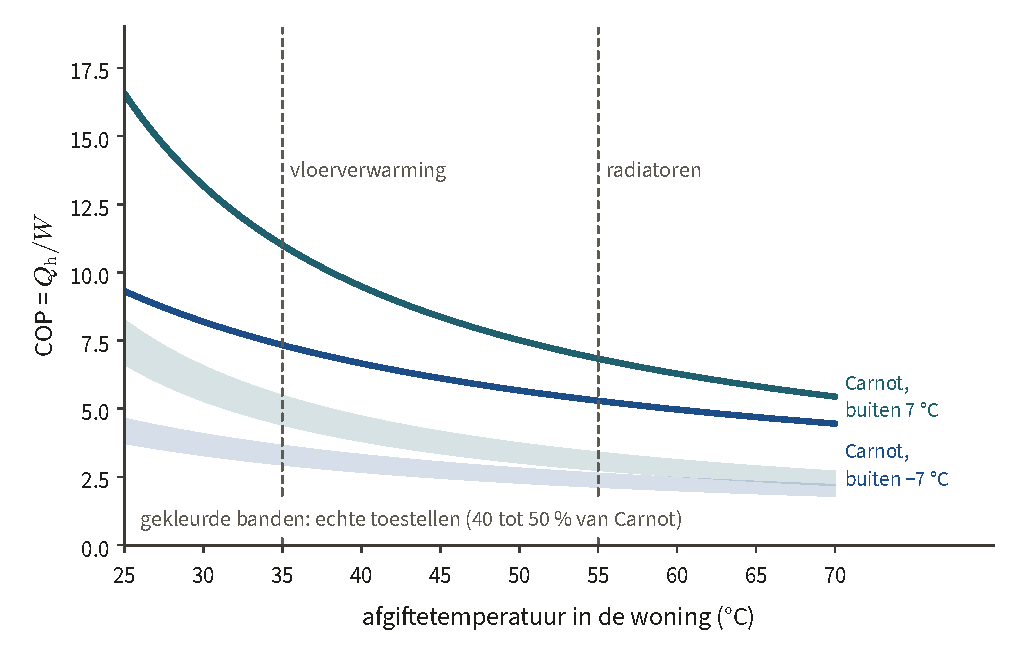
\includegraphics[width=0.75\linewidth]{Figuren/cop_warmtepomp}
    \caption{Maximale COP (Carnot, vergelijking~\eqref{eq:cop-warmtepomp}) van een warmtepomp in functie van de temperatuur waarbij ze de warmte afgeeft, voor een buitentemperatuur van \SI{7}{\celsius} en \SI{-7}{\celsius}. Echte toestellen halen typisch 40 tot \SI{50}{\percent} van de Carnotwaarde, door het temperatuurverschil in de warmtewisselaars en de verliezen in de compressor.}
    \label{fig:cop}
\end{figure}

\begin{casusuitgewerkt}{hoeveel stroom vraagt een warmtepomp?}
\emph{Stap 1: vloerverwarming.} Met $T_\mathrm{h} = \SI{308}{\kelvin}$ en $T_\mathrm{c} = \SI{278}{\kelvin}$:
\[
\mathrm{COP}_\text{max} = \frac{308}{308 - 278} = 10.3, \qquad W_\text{min} = \frac{\SI{10}{\kilo\watt}}{10.3} = \SI{0.97}{\kilo\watt}.
\]
In theorie volstaat dus minder dan een tiende van de warmte als elektriciteit. Het overige komt gratis uit de buitenlucht. Een echt toestel haalt een COP van ongeveer 4 en verbruikt \SI{2.5}{\kilo\watt}.

\emph{Stap 2: radiatoren.} Bij \SI{55}{\celsius} wordt $\mathrm{COP}_\text{max} = 328/50 = 6.6$; in de praktijk ongeveer 3. Dezelfde warmte kost een derde meer stroom. Daarom gaan warmtepompen samen met vloerverwarming en goede isolatie: hoe lager de afgiftetemperatuur, hoe kleiner de sprong die de warmtepomp moet maken.

\emph{Stap 3: de koelmachine van de ammoniakfabriek.} De condensor van hoofdstuk~\ref{ch:energie} (\S\ref{sec:faseovergangen}) moet \SI{15}{\mega\watt} afvoeren bij \SI{-10}{\celsius}, en de koelmachine dumpt die warmte in koelwater van ongeveer \SI{30}{\celsius}. Volgens vergelijking~\eqref{eq:carnot}:
\[
\mathrm{COP}_\text{koel,max} = \frac{263}{303 - 263} = 6.6, \qquad W_\text{min} = \frac{\SI{15}{\mega\watt}}{6.6} = \SI{2.3}{\mega\watt}.
\]
Dat is de vraag uit hoofdstuk~\ref{ch:energie}: waarom de condensor een koelmachine nodig heeft die zelf energie verbruikt. Warmte gaat niet vanzelf van \SI{-10}{\celsius} naar \SI{30}{\celsius}; daarvoor is minstens \SI{2.3}{\mega\watt} arbeid nodig, in de praktijk het dubbele.

\emph{Volgende vraag.} Een gasketel zet \SI{95}{\percent} van de energie van het gas om in warmte, een warmtepomp levert vier keer meer warmte dan ze aan stroom verbruikt. Maar stroom wordt zelf vaak uit gas gemaakt. Wat is dan de beste manier om met een kubieke meter gas een huis te verwarmen?
\end{casusuitgewerkt}

\section{Exergie: de kwaliteit van energie}
\label{sec:exergie}

\begin{casus}{gasketel of warmtepomp?}
Met \SI{1}{\kilo\watt\hour} aardgas levert een condenserende gasketel ongeveer \SI{0.95}{\kilo\watt\hour} warmte. Een moderne gascentrale maakt uit dezelfde \SI{1}{\kilo\watt\hour} gas ongeveer \SI{0.55}{\kilo\watt\hour} elektriciteit. Welke route geeft het meeste warmte in huis? En waarom is het ``zonde'' om gas te verbranden voor water van \SI{35}{\celsius}?

\emph{Schat eerst zelf:} de gasketel verspilt bijna niets. Hoe kan een omweg via een elektriciteitscentrale dan beter zijn?
\end{casus}


De eerste hoofdwet telt energie, de tweede zegt hoeveel ervan bruikbaar is. Hoeveel arbeid kan je maximaal halen uit warmte $Q$ die beschikbaar is bij temperatuur $T$, als de omgeving op $T_0$ staat? We stellen de balansen op voor een machine die die warmte opneemt, arbeid $W$ levert en de rest, $Q_0$, aan de omgeving afgeeft.
\begin{enumerate}
\item \emph{Energiebalans.} Over een kringloop verandert de machine zelf niet, dus $W = Q - Q_0$.
\item \emph{Entropiebalans.} De warme bron verliest $Q/T$ aan entropie, de omgeving wint $Q_0/T_0$. De tweede hoofdwet eist $Q_0/T_0 - Q/T \geq 0$, dus $Q_0 \geq Q\,T_0/T$: de machine \emph{moet} een minimum aan warmte kwijt, om de entropie die met $Q$ binnenkwam af te voeren.
\item \emph{Combineer.} $W = Q - Q_0 \leq Q - Q\,T_0/T$, of
\end{enumerate}
\begin{equation}
W_{\max} = Q\left(1-\frac{T_0}{T}\right).
\label{eq:exergie-warmte}
\end{equation}
Dat is het rendement van Carnot uit \S\ref{sec:carnot}. Het bruikbare deel heet de \emph{exergie} van de warmte, de factor $1 - T_0/T$ de \emph{Carnotfactor}. Figuur~\ref{fig:carnotfactor} toont hoe snel de waarde van warmte daalt met haar temperatuur. Een rivier van \SI{15}{\celsius} bevat enorm veel energie, maar verwarmt geen huis van \SI{20}{\celsius}; daarvoor heb je een warmtepomp nodig, en die verbruikt arbeid. Elektriciteit en arbeid zijn daarentegen zuivere exergie: ze kunnen volledig in elke andere vorm worden omgezet.

Energie gaat nooit verloren, exergie wel: elke irreversibiliteit (wrijving, warmte over een groot temperatuurverschil, menging) vernietigt exergie. Daarom gebruikt men hoogwaardige warmte eerst voor stoom of arbeid, en restwarmte van \SI{80}{\celsius} in een warmtenet. Een warmtewisselaar met een klein temperatuurverschil vernietigt minder exergie, maar vraagt een groter oppervlak: een klassieke ontwerpafweging.


\begin{figure}[htb]
    \centering
    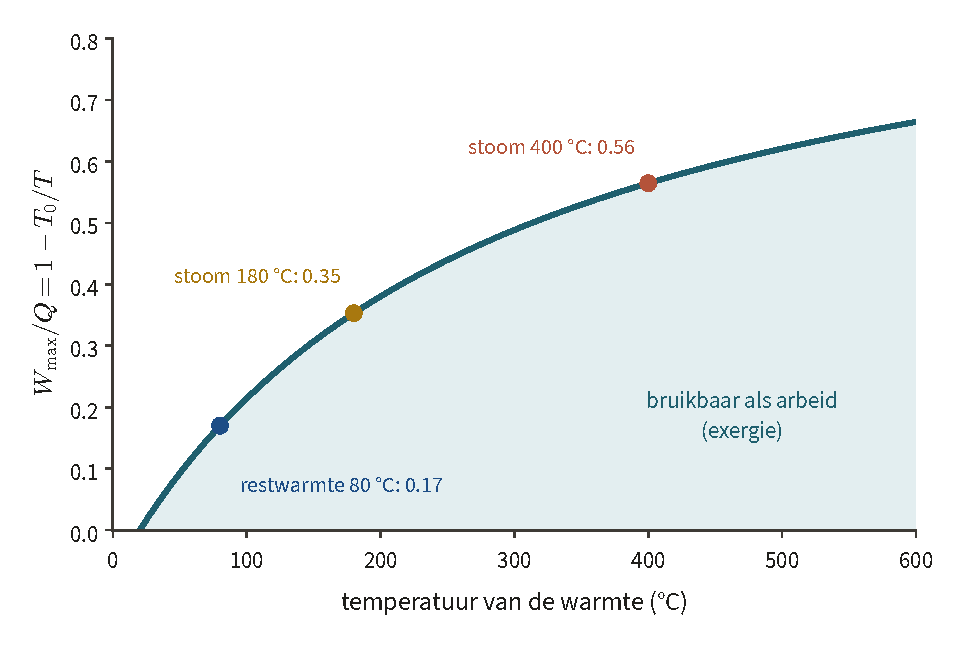
\includegraphics[width=0.7\linewidth]{Figuren/carnotfactor}
    \caption{Maximaal bruikbaar deel van warmte (de Carnotfactor $1 - T_0/T$) in functie van de temperatuur waarbij ze beschikbaar is, voor een omgeving van \SI{20}{\celsius}. Stoom van \SI{400}{\celsius} is voor meer dan de helft omzetbaar in arbeid, restwarmte van \SI{80}{\celsius} voor minder dan een vijfde.}
    \label{fig:carnotfactor}
\end{figure}

\begin{casusuitgewerkt}{gasketel of warmtepomp?}
\emph{Stap 1: de twee routes.} De gasketel levert \SI{0.95}{\kilo\watt\hour} warmte. Via de centrale en een warmtepomp met COP 4 komt er $0.55 \times 4 = \SI{2.2}{\kilo\watt\hour}$ warmte in huis, meer dan het dubbele, ook al gaat in de centrale \SI{45}{\percent} van de energie als restwarmte verloren.

\emph{Stap 2: waarom kan dat?} Kijk naar de exergie. Verbrandingsgassen van zo'n \SI{1500}{\celsius} hebben een Carnotfactor $1 - 278/1773 = 0.84$: bijna alle energie is bruikbaar als arbeid. Water van \SI{35}{\celsius} heeft bij een buitentemperatuur van \SI{5}{\celsius} slechts $1 - 278/308 = 0.10$. De gasketel zet dus hoogwaardige energie om in laagwaardige warmte, en vernietigt daarbij bijna alle exergie, ook al gaat er geen energie verloren. De warmtepomp doet het omgekeerde: ze gebruikt een beetje hoogwaardige energie (elektriciteit, zuivere exergie) om veel laagwaardige warmte uit de buitenlucht op te waarderen.

\emph{Besluit.} Energie gaat nooit verloren, maar haar kwaliteit wel. Wie energie zuinig wil gebruiken, moet de temperatuur van de warmte afstemmen op haar toepassing: hoge temperatuur voor arbeid en processen, lage temperatuur voor verwarming.

\emph{Volgende vraag.} In de buitenunit moet het koelmiddel verdampen bij ongeveer \SI{-5}{\celsius}, onder de temperatuur van de buitenlucht. Waarom kookt de ene stof bij \SI{-42}{\celsius} en de andere bij \SI{100}{\celsius}, en hoe voorspel je dat?
\end{casusuitgewerkt}


\section{De derde hoofdwet van de thermodynamica}
\label{sec:derde-hoofdwet}

Om de entropie van een reactie te berekenen zoals in het voorbeeld van de waterbalans, heb je de entropie van elke stof nodig. Bij de enthalpie konden we enkel verschillen meten, en kozen we een nulpunt per afspraak: $\Delta_fH^\circ = 0$ voor de elementen. Voor entropie blijkt dat niet nodig.

\paragraph{De waarneming.} Walther Nernst mat rond 1906 reacties tussen vaste stoffen bij steeds lagere temperaturen, en stelde vast dat hun reactie-entropie naar nul ging naarmate $T$ naar het absolute nulpunt daalde. Planck trok daaruit de conclusie dat de entropie van elke zuivere, perfect kristallijne stof zelf naar nul gaat.

\begin{definitie}{Derde hoofdwet van de thermodynamica}
De entropie van een perfect kristal van een zuivere stof nadert nul als $T \to \SI{0}{\kelvin}$.
\end{definitie}

Met Boltzmann is dat onmiddellijk duidelijk: in een perfect kristal bij \SI{0}{\kelvin} zit elk atoom op zijn vaste plaats in de laagste energietoestand. Er is precies \'e\'en microtoestand, dus $S = k_B\ln 1 = 0$.

\paragraph{Absolute entropie meten.} Daarmee bestaat er voor entropie een \emph{absolute} schaal. Om de entropie van een stof bij \SI{298}{\kelvin} te kennen, meet men in een calorimeter haar warmtecapaciteit van enkele kelvin tot kamertemperatuur, en telt men alle stukken op, zoals in het voorbeeld van ijs tot stoom:
\[
S_m(T) = \int_0^{T}\frac{C_p}{T}\,\dd T + \sum \frac{\Delta H_\text{trans}}{T_\text{trans}} .
\]
Het allerlaatste stukje, onder de laagste meettemperatuur, wordt geschat met de wet van Debye, $C_p \propto T^3$. De waarde bij \SI{298.15}{\kelvin} en \SI{1}{\bar} heet de \emph{standaardmolaire entropie} $S_m^\circ$ (tabel~\ref{tab:standaardentropie}). Let op: ook een element heeft bij kamertemperatuur een positieve $S_m^\circ$, door translatie, rotatie en vibratie van zijn moleculen (\S~\ref{sec:moleculaire-beweging}), terwijl zijn $\Delta_fH^\circ$ per afspraak nul is.

Niet elke stof is bij \SI{0}{\kelvin} een perfect kristal. In vast koolstofmonoxide kan elke molecule als CO of als OC in het rooster liggen, omdat beide uiteinden bijna even groot zijn. Met twee keuzes per molecule blijft er bij \SI{0}{\kelvin} een \emph{restentropie} $R\ln 2 = \SI{5.8}{\joule\per\mole\per\kelvin}$ over; gemeten wordt \SI{4.6}{\joule\per\mole\per\kelvin}, omdat de ori\"entaties niet helemaal willekeurig zijn. Een mooie bevestiging dat de entropie van Clausius en die van Boltzmann dezelfde grootheid zijn.

\begin{table}[htb]
\centering
\caption{Standaardmolaire entropie $S_m^\circ$ (\SI{298.15}{\kelvin}, \SI{1}{\bar}) voor de stoffen van de ammoniaksynthese. Bron: NIST Chemistry WebBook, NIST Standard Reference Database 69.}
\label{tab:standaardentropie}
\begin{tabular}{lc}
\toprule
Stof & $S_m^\circ$ (\si{\joule\per\mole\per\kelvin}) \\
\midrule
$\mathrm{N_2(g)}$ & 191.6 \\
$\mathrm{H_2(g)}$ & 130.7 \\
$\mathrm{NH_3(g)}$ & 192.8 \\
\bottomrule
\end{tabular}
\end{table}

De reactie-entropie volgt, net als de reactie-enthalpie met de wet van Hess, uit
\begin{equation}
\boxed{\Delta_r S^\circ = \sum_i \nu_i\,S_{m,i}^\circ}
\label{eq:reactie-entropie}
\end{equation}
met $\nu_i$ positief voor producten en negatief voor reagentia.

\begin{voorbeeld}{Reactie-entropie van de ammoniaksynthese}
Voor \ce{N2(g) + 3 H2(g) <=> 2 NH3(g)} geeft tabel~\ref{tab:standaardentropie}:
\[
\Delta_r S^\circ = 2(192.8) - [191.6 + 3(130.7)] = 385.6 - 583.7 = \SI{-198.1}{\joule\per\mole\per\kelvin}.
\]
Sterk negatief: vier mol gas worden er twee, met veel minder bewegingsvrijheid. Een vuistregel die je hier ziet: de entropieverandering van een reactie wordt bijna volledig bepaald door de verandering van het aantal mol gas. Elke mol gas die verdwijnt, kost ongeveer \SI{100}{\joule\per\kelvin}. In de volgende sectie zien we wat dat betekent voor de temperatuur waarbij de ammoniakreactor kan werken.
\end{voorbeeld}

\section{De Gibbs-vrije energie en het thermodynamisch evenwicht}
\label{sec:gibbs}

\begin{casus}{bij welke temperatuur kookt het koelmiddel?}
Moderne warmtepompen gebruiken propaan (R290) als koelmiddel. Bij \SI{1}{\bar} is de verdampingsenthalpie van propaan \SI{19.0}{\kilo\joule\per\mole} en de verdampingsentropie \SI{82}{\joule\per\mole\per\kelvin}. Bij welke temperatuur kookt het? En is dat geschikt om warmte op te nemen uit buitenlucht van \SI{5}{\celsius}?

\emph{Schat eerst zelf:} verdampen kost enthalpie, maar levert entropie op. Bij lage temperatuur wint de enthalpie, bij hoge de entropie. Waar ligt het kantelpunt?
\end{casus}


\subsection{De ingenieursvisie: het systeem en zijn omgeving}

Bij de tweede hoofdwet moesten we telkens de entropie van het universum berekenen: het systeem plus de omgeving. Voor de natuur bestaat er geen grens tussen beide, maar voor een ingenieur wel. Hij kent zijn reactor, kolom of warmtewisselaar goed: de samenstelling, de temperatuur, de druk. Van de omgeving weet hij veel minder: waar gaat de warmte precies heen, en wat gebeurt er daar mee?

Daar zit een praktisch probleem. De richting van een proces wordt bepaald door een grootheid van het hele universum, terwijl de ingenieur enkel het systeem kent. De vraag is dus of er een grootheid bestaat die je volledig uit eigenschappen van het \emph{systeem} kan berekenen, maar die toch zegt in welke richting het proces loopt. Josiah Willard Gibbs toonde in 1876 dat dat kan, voor het geval dat in de chemie en procestechniek bijna altijd geldt: constante temperatuur en constante druk.

\subsection{De Gibbs-vrije energie}

\begin{definitie}{Gibbs-vrije energie}
\begin{equation}
G = H - TS.
\end{equation}
Bij constante temperatuur en druk geldt: $\Delta G < 0$ spontaan, $\Delta G = 0$ evenwicht, $\Delta G > 0$ niet spontaan (de omgekeerde richting is dan spontaan).
\end{definitie}

$G$ is geen nieuwe vorm van energie. Het is een slim gekozen combinatie van grootheden die we al kennen, die de omgeving ongemerkt meerekent. Dat zien we in de afleiding.

\subsubsection{Afleiding uit de tweede hoofdwet}

We vertrekken van de tweede hoofdwet en werken de omgeving weg, in vier stappen.
\begin{enumerate}
\item \emph{Splits het universum.} Voor een klein stapje van het proces eist de tweede hoofdwet
\[
\dd S_\text{univ} = \dd S + \dd S_\text{omg} \geq 0,
\]
met $\dd S$ de entropieverandering van het systeem.
\item \emph{Druk de omgeving uit in het systeem.} Bij constante druk is de warmte die het systeem opneemt gelijk aan $\dd H$ (hoofdstuk~\ref{ch:energie}). De omgeving ontvangt dus $-\dd H$. Ze is een groot reservoir op temperatuur $T$, zodat $\dd S_\text{omg} = -\dd H/T$, zoals bij de lokale entropieafname.
\item \emph{Vul in.} $\dd S - \dd H/T \geq 0$. Nu staan er enkel nog eigenschappen van het systeem.
\item \emph{Vermenigvuldig met $-T$.} Omdat $T > 0$ keert het ongelijkheidsteken om: $\dd H - T\,\dd S \leq 0$. Bij constante temperatuur is $\dd H - T\,\dd S$ precies $\dd(H - TS) = \dd G$, dus
\[
\dd G \leq 0 \qquad (\text{constante } T \text{ en } p).
\]
\end{enumerate}
Een daling van $G$ van het systeem is dus hetzelfde als een stijging van de entropie van het universum: $\Delta G = -T\Delta S_\text{univ}$. De Gibbs-vrije energie is geen nieuwe natuurwet, maar de tweede hoofdwet, herschreven in eigenschappen van het systeem. De term $\Delta H$ staat voor wat er in de omgeving gebeurt, de term $T\Delta S$ voor wat er in het systeem gebeurt.

Het woord ``vrij'' heeft ook een concrete betekenis: $-\Delta G$ is de maximale nuttige arbeid, naast de volumearbeid tegen de atmosfeer, die een proces bij constante $T$ en $p$ kan leveren. Een brandstofcel of batterij zet $-\Delta G$ om in elektrische arbeid (hoofdstuk~\ref{ch:elektrochemie}), niet $-\Delta H$.

\begin{voorbeeld}{Werkt de ammoniakreactor bij elke temperatuur?}
Voor \ce{N2 + 3 H2 -> 2 NH3} is $\Delta_r H^\circ = \SI{-92.2}{\kilo\joule\per\mole}$ (hoofdstuk~\ref{ch:energie}) en $\Delta_r S^\circ = \SI{-198.1}{\joule\per\mole\per\kelvin}$. Bij \SI{298}{\kelvin}:
\[
\Delta_r G^\circ = \Delta_r H^\circ - T\Delta_r S^\circ = -92.2 - (298)(-0.1981) = -92.2 + 59.0 = \SI{-33.2}{\kilo\joule\per\mole}.
\]
De reactie is bij kamertemperatuur spontaan. De twee termen werken echter tegen elkaar: de enthalpie is gunstig, de entropie ongunstig. Bij hogere temperatuur weegt de entropieterm zwaarder, en bij
\[
T^* = \frac{\Delta_r H^\circ}{\Delta_r S^\circ} = \frac{-92\,200}{-198.1} = \SI{465}{\kelvin} \approx \SI{190}{\celsius}
\]
wordt $\Delta_r G^\circ$ nul. De katalysator werkt pas goed bij 400 tot \SI{500}{\celsius}, ruim boven $T^*$: daar is $\Delta_r G^\circ$ positief. Dat de fabriek toch ammoniak maakt, komt door de hoge druk van \SI{200}{\bar}. Hoe druk en temperatuur samen de opbrengst bepalen, is het onderwerp van hoofdstuk~\ref{ch:reagerend}.
\end{voorbeeld}

\subsubsection{De fundamentele vergelijkingen}
\label{sec:fundamentele-vgl}

Hoe verandert $G$ als je de temperatuur of de druk verandert? Dat volgt uit de combinatie van de eerste en de tweede hoofdwet. We bouwen het op in drie stappen, telkens met de productregel.

\paragraph{Stap 1: de interne energie.} Voor een gesloten systeem dat enkel volumearbeid uitwisselt, geeft de eerste hoofdwet voor een reversibele verandering $\dd U = \delta Q_\text{rev} - p\,\dd V$. Met Clausius is $\delta Q_\text{rev} = T\,\dd S$:
\begin{equation}
\boxed{\dd U = T\,\dd S - p\,\dd V}
\label{eq:fundU}
\end{equation}
We leidden dit af langs een reversibele weg, maar het geldt voor elke verandering: $U$, $S$ en $V$ zijn toestandsfuncties, en het verband tussen hun veranderingen hangt niet af van hoe je van de ene toestand naar de andere gaat.

\paragraph{Stap 2: de enthalpie.} Met $H = U + pV$ geeft de productregel $\dd H = \dd U + p\,\dd V + V\,\dd p$. Vul vergelijking~\eqref{eq:fundU} in:
\begin{equation}
\dd H = (T\,\dd S - p\,\dd V) + p\,\dd V + V\,\dd p = T\,\dd S + V\,\dd p.
\label{eq:fundH}
\end{equation}

\paragraph{Stap 3: de Gibbs-vrije energie.} Met $G = H - TS$ geeft de productregel $\dd G = \dd H - T\,\dd S - S\,\dd T$. Vul vergelijking~\eqref{eq:fundH} in:
\[
\dd G = (T\,\dd S + V\,\dd p) - T\,\dd S - S\,\dd T,
\]
zodat
\begin{equation}\label{eq:fundG}
\boxed{\dd G = V\,\dd p - S\,\dd T}
\end{equation}

\paragraph{Wat zegt deze vergelijking?} Ze geeft twee concrete regels.
\begin{itemize}
\item Bij constante druk is $(\partial G/\partial T)_p = -S$. Warm je een stof op, dan daalt haar $G$, en sneller naarmate haar entropie groter is. Een gas daalt dus sneller dan een vloeistof, en een vloeistof sneller dan een vaste stof. Daarom wint bij hoge temperatuur altijd de fase met de hoogste entropie (\S\ref{sec:mu-p-T}).
\item Bij constante temperatuur is $(\partial G/\partial p)_T = V$. Verhoog je de druk, dan stijgt $G$, en sterker naarmate het volume groter is. Voor een gas is dat effect groot, voor een vloeistof of vaste stof klein. Daarom verschuift hoge druk een evenwicht naar de kant met minder mol gas, zoals bij de ammoniaksynthese.
\end{itemize}
In hoofdstuk~\ref{ch:niet-reagerend} levert vergelijking~\eqref{eq:fundG} de chemische potentiaal als functie van druk en samenstelling, en in hoofdstuk~\ref{ch:reagerend} de vergelijking van Van 't Hoff.

\subsection{De competitie tussen enthalpie en entropie}

In $\Delta G = \Delta H - T\Delta S$ trekken twee tendensen aan het systeem. Het wil zijn enthalpie verlagen: sterke bindingen en gunstige intermoleculaire interacties. En het wil naar toestanden met meer microtoestanden: hogere entropie. De temperatuur bepaalt het gewicht van de tweede tendens. Bij lage $T$ beslist vooral $\Delta H$, bij hoge $T$ vooral $\Delta S$. Volgens de tekens van $\Delta H$ en $\Delta S$ zijn er vier gevallen (figuur~\ref{fig:dG-temperatuur}):
\begin{itemize}
\item $\Delta H < 0$ en $\Delta S > 0$: altijd spontaan (ontbinding van waterstofperoxide);
\item $\Delta H > 0$ en $\Delta S < 0$: nooit spontaan (ozon vormen uit zuurstof);
\item $\Delta H < 0$ en $\Delta S < 0$: spontaan \emph{onder} $T^* = \Delta H/\Delta S$ (ammoniaksynthese, bevriezen);
\item $\Delta H > 0$ en $\Delta S > 0$: spontaan \emph{boven} $T^*$ (kalk branden, smelten, verdampen).
\end{itemize}

\begin{figure}[htb]
    \centering
    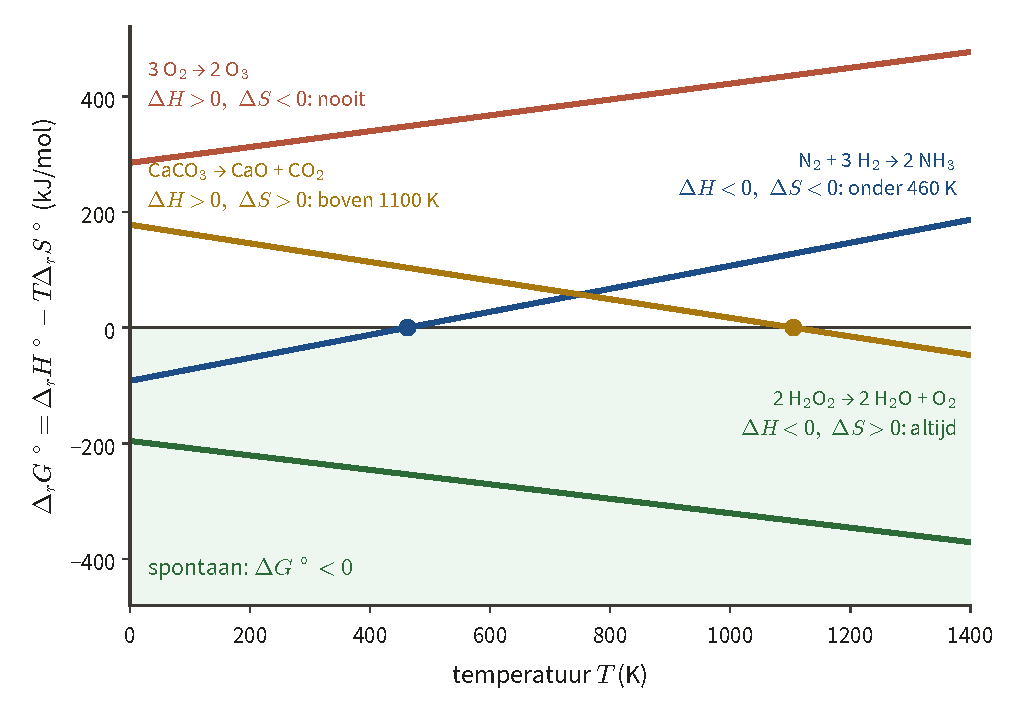
\includegraphics[width=0.75\linewidth]{Figuren/dG_temperatuur}
    \caption{$\Delta_r G^\circ$ in functie van de temperatuur voor vier reacties, \'e\'en per tekencombinatie van $\Delta_r H^\circ$ en $\Delta_r S^\circ$. De helling is $-\Delta_r S^\circ$, het snijpunt met de verticale as $\Delta_r H^\circ$. De bolletjes markeren $T^* = \Delta_r H^\circ/\Delta_r S^\circ$, waar de reactie van richting wisselt (standaardwaarden bij \SI{298}{\kelvin}, constant verondersteld).}
    \label{fig:dG-temperatuur}
\end{figure}

\begin{voorbeeld}{De smelttemperatuur van water}
Bij het smelten van ijs moeten waterstofbruggen gedeeltelijk worden verbroken. Dat kost energie: $\Delta H_\text{fus} = \SI{6.01}{\kilo\joule\per\mole}$, de omgeving moet warmte leveren en haar entropie daalt. Tegelijk krijgen de watermoleculen in de vloeistof veel meer bewegingsvrijheid: $\Delta S_\text{fus} = \SI{22.0}{\joule\per\mole\per\kelvin}$. Welke tendens wint, hangt af van de temperatuur:
\begin{itemize}
\item bij \SI{-10}{\celsius}: $\Delta G_\text{fus} = 6010 - (263)(22.0) = \SI{+224}{\joule\per\mole}$, ijs blijft ijs;
\item bij \SI{+10}{\celsius}: $\Delta G_\text{fus} = 6010 - (283)(22.0) = \SI{-216}{\joule\per\mole}$, ijs smelt;
\item het kantelpunt ligt waar $\Delta G_\text{fus} = 0$: $T_\text{fus} = \Delta H_\text{fus}/\Delta S_\text{fus} = 6010/22.0 = \SI{273}{\kelvin}$.
\end{itemize}
Het smeltpunt is dus precies de temperatuur waar enthalpie en entropie elkaar in evenwicht houden. Bij lage temperatuur weegt de entropiewinst te licht om de smeltwarmte te betalen; bij hoge temperatuur wint ze.
\end{voorbeeld}

\subsection{Spontaniteit is niet snelheid}

Spontaniteit zegt iets over de \emph{richting}, niet over de \emph{snelheid}. Diamant zou spontaan in grafiet moeten overgaan ($\Delta G < 0$), maar bij kamertemperatuur gebeurt dat in geen miljard jaar. Methaan en zuurstof kunnen jarenlang samen in een tank zitten; pas een vonk zet de verbranding in gang. Hoe snel een spontaan proces verloopt, is het onderwerp van de kinetiek (hoofdstuk~\ref{ch:kinetiek}).

\subsection{Het thermodynamisch evenwicht}

Een systeem bij constante $T$ en $p$ evolueert zoals een bal in een berglandschap: bergaf in $G$, tot in de vallei. In dat minimum is er geen drijvende kracht meer: het systeem is in evenwicht. Voor fase-evenwichten en mengsels werken we dat uit in hoofdstuk~\ref{ch:niet-reagerend}, voor chemische reacties in hoofdstuk~\ref{ch:reagerend}.

\begin{casusuitgewerkt}{bij welke temperatuur kookt het koelmiddel?}
Verdampen is spontaan zodra $\Delta G_\text{vap} = \Delta H_\text{vap} - T\Delta S_\text{vap} < 0$. Het kookpunt is de temperatuur waarbij beide termen elkaar opheffen:
\[
T_b = \frac{\Delta H_\text{vap}}{\Delta S_\text{vap}} = \frac{19\,000}{82} = \SI{232}{\kelvin} = \SI{-41}{\celsius}.
\]
Gemeten: \SI{-42}{\celsius}. Bij \SI{1}{\bar} kookt propaan dus ruim onder de buitentemperatuur: het neemt gretig warmte op uit lucht van \SI{5}{\celsius}, zelfs uit lucht van \SI{-20}{\celsius}. In de buitenunit werkt men bij een iets hogere druk, ongeveer \SI{4}{\bar}, zodat het kookpunt naar \SI{-5}{\celsius} schuift; hoe het kookpunt met de druk verandert, volgt in hoofdstuk~\ref{ch:niet-reagerend}. In de condensor perst de compressor het koelmiddel tot ongeveer \SI{12}{\bar}, waar het pas bij zo'n \SI{35}{\celsius} condenseert en zijn warmte aan de vloerverwarming afgeeft.

De verdampingsentropie van \SI{82}{\joule\per\mole\per\kelvin} is geen toeval: bijna alle vloeistoffen winnen bij verdampen ongeveer evenveel microtoestanden (regel van Trouton, hoofdstuk~\ref{ch:intermoleculair}). Een koelmiddel kies je dus vooral via zijn verdampingsenthalpie, dus via de sterkte van de krachten tussen zijn moleculen.
\end{casusuitgewerkt}


\section{De chemische potentiaal}
\label{sec:chemische-potentiaal}

Tot nu toe bekeken we een systeem als geheel. Processen bevatten echter zelden \'e\'en zuivere stof. In een reactor, een destillatiekolom of een absorber verandert de hoeveelheid van elke component afzonderlijk: ammoniak ontstaat, ethanol verdampt sneller dan water, \ce{CO2} lost op in een solvent. We hebben dus een drijvende kracht \emph{per component} nodig.

\paragraph{Een potentiaal voor materie.} Elke spontane stroom in de natuur wordt gedreven door een verschil in een potentiaal, en stopt wanneer dat verschil verdwijnt:
\begin{center}
\begin{tabular}{lll}
\toprule
wat stroomt & drijvende kracht & evenwicht als \\
\midrule
water in een rivier & hoogteverschil & gelijke hoogte \\
elektrische lading & spanningsverschil & gelijke potentiaal \\
warmte & temperatuurverschil & gelijke $T$ \\
een fluïdum & drukverschil & gelijke $p$ \\
materie (diffusie, faseovergang, reactie) & verschil in chemische potentiaal & gelijke $\mu$ \\
\bottomrule
\end{tabular}
\end{center}

\paragraph{Definitie.} De chemische potentiaal van component $i$ is
\begin{equation}
\mu_i = \left(\frac{\partial G}{\partial n_i}\right)_{T,p,n_{j\neq i}} .
\end{equation}
In woorden: met hoeveel stijgt de Gibbs-vrije energie van het systeem als je een kleine hoeveelheid van component $i$ toevoegt, bij constante temperatuur, druk en hoeveelheden van de andere componenten? Voor een zuivere stof is dat gewoon de molaire Gibbs-vrije energie, $\mu = G_m$.

\paragraph{Waarom stroomt materie naar lage $\mu$?} Stel dat \SI{1}{\milli\mole} van component $i$ overgaat van fase $\alpha$ naar fase $\beta$, bijvoorbeeld van vloeistof naar damp. De Gibbs-vrije energie van fase $\alpha$ daalt met $\mu_i^\alpha \times \SI{1}{\milli\mole}$, die van fase $\beta$ stijgt met $\mu_i^\beta \times \SI{1}{\milli\mole}$. Samen is $\dd G = (\mu_i^\beta - \mu_i^\alpha)\,\dd n_i$. Volgens het criterium $\dd G < 0$ gebeurt dat enkel vanzelf als $\mu_i^\beta < \mu_i^\alpha$. Een component verplaatst zich dus spontaan van hoge naar lage chemische potentiaal, net zoals warmte van hoge naar lage temperatuur.

\paragraph{Het criterium voor evenwicht.} De overgang stopt wanneer $\mu_i^\alpha = \mu_i^\beta$: dan levert een verschuiving geen daling van $G$ meer op. In evenwicht is de chemische potentiaal van elke component overal gelijk. Water in een gesloten vat is in evenwicht met zijn damp als $\mu^\text{vloeistof} = \mu^\text{damp}$; een opgeloste stof diffundeert tot $\mu$ overal gelijk is; een reactie loopt tot de chemische potentialen van reagentia en producten, gewogen met hun stoichiometrische co\"effici\"enten, in balans zijn.

Hoe $\mu$ verandert met de temperatuur, de druk en de samenstelling van een mengsel, waarom het smeltpunt en het kookpunt precies de punten zijn waar twee fasen dezelfde $\mu$ hebben, en hoe je zo dampdrukken, oplosbaarheden en evenwichtsconstanten berekent, volgt in hoofdstuk~\ref{ch:niet-reagerend} (fase-evenwichten en mengsels) en hoofdstuk~\ref{ch:reagerend} (chemische evenwichten).

\section{De warmtepomp opnieuw bekeken}

Met de begrippen uit dit hoofdstuk kan je de vragen uit het begin beantwoorden:
\begin{itemize}
\item \emph{Waarom warmte niet vanzelf naar binnen stroomt} (\S\ref{sec:waarschijnlijkheid-entropie}): een gelijkmatige verdeling van de energie heeft overweldigend veel meer microtoestanden. De entropie, $S = k_B\ln\Omega$, meet dat aantal, en de tweede hoofdwet zegt dat ze in totaal nooit daalt.
\item \emph{Hoeveel stroom} (\S\ref{sec:tweedehoofdwet}): uit de entropiebalans volgt $\mathrm{COP} \leq T_\mathrm{h}/(T_\mathrm{h} - T_\mathrm{c})$. Voor vloerverwarming bij \SI{5}{\celsius} buiten is dat 10, in de praktijk ongeveer 4. Dezelfde redenering geeft de minimale arbeid voor de koelmachine van de ammoniakfabriek: \SI{2.3}{\mega\watt}.
\item \emph{Gasketel of warmtepomp} (\S\ref{sec:exergie}): niet de hoeveelheid energie telt, maar haar kwaliteit. Gas verbranden voor water van \SI{35}{\celsius} vernietigt bijna alle exergie; via elektriciteit en een warmtepomp komt er twee keer meer warmte in huis.
\item \emph{Het koelmiddel} (\S\ref{sec:gibbs}): de stof kookt waar $\Delta G_\text{vap} = 0$, dus bij $T_b = \Delta H_\text{vap}/\Delta S_\text{vap}$. Hetzelfde criterium, $\Delta G < 0$, bepaalt of een reactie vanzelf verloopt.
\end{itemize}
Het criterium $\Delta G \leq 0$, of in een mengsel gelijke chemische potentialen, is de rode draad van de volgende hoofdstukken: fase-evenwichten en mengsels (hoofdstuk~\ref{ch:niet-reagerend}), chemische evenwichten (hoofdstuk~\ref{ch:reagerend}) en elektrochemie (hoofdstuk~\ref{ch:elektrochemie}).

\newpage
\section{Oefeningen}

% Oefeningen bij dit hoofdstuk (ingevoegd achteraan het hoofdstuk met \input).
% Een oefening:  \begin{oefening}[titel] ... \end{oefening}   (boek en website)
% De oplossing:  \begin{oplossing} ... \end{oplossing}       (enkel website, dichtgeklapt)

Neem $R = \SI{8.314}{\joule\per\mole\per\kelvin}$ en $p^\circ = \SI{1}{\bar}$.

\begin{oefening}[Mengentropie van een driecomponent-mengsel]
Een vat bevat aanvankelijk \(1\,\mathrm{mol}\) stikstof, \(1\,\mathrm{mol}\) zuurstof en \(1\,\mathrm{mol}\) argon, elk in afzonderlijke compartimenten bij gelijke temperatuur en druk. De compartimenten worden geopend en de gassen mengen spontaan.

\begin{enumerate}
\item[(a)]
  Bereken de mengentropie per mol mengsel.
\item[(b)]
  Bereken de bijbehorende verandering van de Gibbs-vrije energie bij \(298\,\mathrm{K}\).
\item[(c)]
  Hoeveel minimale arbeid is nodig om het mengsel bij \(298\,\mathrm{K}\) terug te scheiden in de drie zuivere componenten?
\end{enumerate}

\emph{Hint:} \(\Delta S_{\text{meng}} = -R\sum_i x_i \ln x_i\); \(\Delta G_{\text{meng}} = -T \Delta S_{\text{meng}}\) voor ideale mengsels.
\end{oefening}
\begin{oplossing}
\textbf{Resultaat:} (a) \(\Delta S_{\text{meng}}\) = \textbf{9.13 J/(mol\ensuremath{\cdot{}}K)} (27.4 J/K in totaal). (b) \(\Delta G_{\text{meng}}\) = \textbf{\ensuremath{-}2.72 kJ/mol} (\ensuremath{-}8.17 kJ). (c) \(W_{\min}\) = \textbf{8.17 kJ}.

\textbf{(a)} Met \(x_i = 1/3\): \(\Delta S_{\text{meng}} = -R \cdot 3 \cdot \frac{1}{3}\ln\frac{1}{3} = R\ln 3 = 9.13\,\mathrm{J/(mol\cdot K)}\) per mol mengsel, of \(27.4\,\mathrm{J/K}\) voor de 3 mol samen.

\textbf{(b)} \(\Delta G_{\text{meng}} = -T\Delta S_{\text{meng}} = -(298)(9.13) = -2.72\,\mathrm{kJ/mol}\) mengsel, of \(-8.17\,\mathrm{kJ}\) in totaal. Negatief: mengen verloopt spontaan.

\textbf{(c)} Scheiden is het omgekeerde proces met \(\Delta G = +8.17\,\mathrm{kJ}\). De minimale (reversibele) arbeid bedraagt dus \(8.17\,\mathrm{kJ}\). Echte scheidingsprocessen (cryogene luchtscheiding, membranen) verbruiken daar een veelvoud van; deze ondergrens toont hoeveel ruimte er theoretisch is voor energiebesparing.
\end{oplossing}

\begin{oefening}[Entropie bij faseovergangen]
Thallium smelt bij \(304\,^\circ\mathrm{C}\) met een smeltenthalpie van \(\Delta H_{\text{fus}} = 4.27\,\mathrm{kJ/mol}\).

\begin{enumerate}
\item[(a)]
  Bereken de smeltentropie.
\item[(b)]
  Verklaar vanuit de orde-grootte waarom deze entropie kleiner is dan de verdampingsentropie van water (\(\Delta S_{\text{vap}} \approx 109\,\mathrm{J/(mol\cdot K)}\)).
\item[(c)]
  Bereken de verandering van de Gibbs-vrije energie bij het smelten precies op het smeltpunt.
\end{enumerate}
\end{oefening}
\begin{oplossing}
\textbf{Resultaat:} (a) \(\Delta S_{\text{fus}}\) = \textbf{7.40 J/(mol\ensuremath{\cdot{}}K)}. (c) Op het smeltpunt is \(\Delta G_{\text{fus}}\) = \textbf{0}.

\textbf{(a)} \(\Delta S_{\text{fus}} = \Delta H_{\text{fus}}/T_{\text{fus}} = 4270/577.15 = 7.40\,\mathrm{J/(mol\cdot K)}\).

\textbf{(b)} Bij smelten blijven de atomen dicht opeengepakt: de vloeistof is slechts iets wanordelijker dan het kristal, zodat het aantal toegankelijke microtoestanden weinig toeneemt. Bij verdampen neemt het beschikbare volume per molecule met een factor duizend toe, en bij water wordt bovendien het geordende waterstofbrugnetwerk verbroken. Daarom is \(\Delta S_{\text{vap}}\) typisch een grootteorde groter dan \(\Delta S_{\text{fus}}\).

\textbf{(c)} Op het smeltpunt zijn vaste stof en vloeistof in evenwicht: \(\Delta G_{\text{fus}} = \Delta H_{\text{fus}} - T_{\text{fus}}\Delta S_{\text{fus}} = 0\).
\end{oplossing}

\begin{oefening}[Spontaniteitscriterium: smelten van ijs bij verschillende temperaturen]
Voor het smelten van ijs geldt \(\Delta H_{\text{fus}} = 6.0\,\mathrm{kJ/mol}\) en \(\Delta S_{\text{fus}} = 22.0\,\mathrm{J/(mol\cdot K)}\) (verondersteld constant).

\begin{enumerate}
\item[(a)]
  Bereken \(\Delta G\) bij \(-10\,^\circ\mathrm{C}\), \(0\,^\circ\mathrm{C}\) en \(+10\,^\circ\mathrm{C}\).
\item[(b)]
  Bepaal bij welke temperatuur ijs en vloeibaar water in evenwicht zijn.
\item[(c)]
  Verklaar vanuit het teken van \(\Delta G\) waarom ijs bij \(-10\,^\circ\mathrm{C}\) niet spontaan smelt.
\end{enumerate}
\end{oefening}
\begin{oplossing}
\textbf{Resultaat:} (a) \(\Delta G\) = \textbf{+211}, \textbf{\ensuremath{\approx{}} 0} en \textbf{\ensuremath{-}229 J/mol} bij 263, 273 en 283 K. (b) \(T\) = \textbf{272.7 K} (\ensuremath{\approx{}} 0 °C). (c) Bij \ensuremath{-}10 °C is \textbf{bevriezen} spontaan.

\textbf{(a)} Met \(\Delta G = \Delta H - T\Delta S\):

\begin{center}
\begin{tabular}{ll}
\toprule
\(T\) & \(\Delta G\) (J/mol) \\
\midrule
\(263.15\,\mathrm{K}\) & \(+211\) \\
\(273.15\,\mathrm{K}\) & \(-9\) (\ensuremath{\approx{}} 0) \\
\(283.15\,\mathrm{K}\) & \(-229\) \\
\bottomrule
\end{tabular}
\end{center}

\textbf{(b)} \(\Delta G = 0\) bij \(T = \Delta H/\Delta S = 6000/22.0 = 272.7\,\mathrm{K}\), of \(-0.4\,^\circ\mathrm{C}\). Het kleine verschil met \(0\,^\circ\mathrm{C}\) komt door de afronding van de gegevens.

\textbf{(c)} Bij \(-10\,^\circ\mathrm{C}\) is \(\Delta G > 0\): de enthalpiekost van het smelten weegt zwaarder dan de entropiewinst \(T\Delta S\). Het omgekeerde proces, bevriezen, is dan spontaan. Daarom strooit men zout op wegen: zout verlaagt de chemische potentiaal van het vloeibare water (hoofdstuk 5), waardoor het smeltpunt daalt.
\end{oplossing}

\begin{oefening}[Evenwichtsconstante en standaardreactie-Gibbsenergie]
Voor de reactie

\[
\mathrm{N_2O_4(g) \rightleftharpoons 2\,NO_2(g)}
\]

bedraagt \(\Delta_r G^\circ = +4.8\,\mathrm{kJ/mol}\) bij \(298\,\mathrm{K}\).

\begin{enumerate}
\item[(a)]
  Bereken de evenwichtsconstante \(K\) bij \(298\,\mathrm{K}\).
\item[(b)]
  Is de reactie bij standaardomstandigheden spontaan in de voorwaartse richting?
\item[(c)]
  Bij welke waarde van het reactiequotiënt \(Q\) zou de reactie precies in evenwicht zijn?
\end{enumerate}
\end{oefening}
\begin{oplossing}
\textbf{Resultaat:} (a) \(K\) = \textbf{0.144}. (b) \textbf{Nee}, bij \(Q = 1\) verloopt de reactie naar links. (c) Evenwicht bij \(Q = K\) = \textbf{0.144}.

\textbf{(a)} \(K = \exp(-\Delta_r G^\circ/RT) = \exp\!\left(-\dfrac{4800}{(8.314)(298)}\right) = 0.144\).

\textbf{(b)} Nee. Bij standaardomstandigheden (beide gassen bij \(1\,\mathrm{bar}\), dus \(Q = 1\)) is \(\Delta_r G = \Delta_r G^\circ > 0\): de reactie verloopt spontaan in de \emph{omgekeerde} richting tot het evenwicht bereikt is. Dat betekent niet dat er geen \(\mathrm{NO_2}\) gevormd wordt: vertrekkend van zuiver \(\mathrm{N_2O_4}\) (\(Q = 0\)) dissocieert een deel wel degelijk.

\textbf{(c)} Evenwicht wanneer \(\Delta_r G = \Delta_r G^\circ + RT\ln Q = 0\), dus \(Q = K = 0.144\).
\end{oplossing}

\begin{oefening}[Invloed van temperatuur: de vergelijking van Van 't Hoff]
Voor de ammoniaksynthese \(\mathrm{N_2 + 3\,H_2 \rightleftharpoons 2\,NH_3}\) bedraagt \(\Delta_r H^\circ = -92.4\,\mathrm{kJ/mol}\) en \(\Delta_r G^\circ = -33.0\,\mathrm{kJ/mol}\) bij \(298\,\mathrm{K}\).

\begin{enumerate}
\item[(a)]
  Bereken \(K\) bij \(298\,\mathrm{K}\).
\item[(b)]
  Schat \(K\) bij \(700\,\mathrm{K}\) (veronderstel \(\Delta_r H^\circ\) constant). Gebruik de geïntegreerde vorm van Van 't Hoff.
\item[(c)]
  Verklaar vanuit het teken van \(\Delta_r H^\circ\) waarom de evenwichtsconstante daalt bij stijgende temperatuur.
\item[(d)]
  Combineer met Hoofdstuk 1: bereken ook \(\Delta_r S^\circ\) bij \(298\,\mathrm{K}\).
\end{enumerate}
\end{oefening}
\begin{oplossing}
\textbf{Resultaat:} (a) \(K_{298}\) = \textbf{6.1\ensuremath{\cdot{}}10\ensuremath{^{5}}}. (b) \(K_{700}\) = \textbf{3.0\ensuremath{\cdot{}}10\ensuremath{^{-4}}}. (c) Exotherm: \(K\) \textbf{daalt} met \(T\). (d) \(\Delta_r S^\circ\) = \textbf{\ensuremath{-}199 J/(mol\ensuremath{\cdot{}}K)}.

\textbf{(a)} \(\ln K = 33\,000/(8.314 \times 298) = 13.32\), dus \(K = 6.1\times10^{5}\).

\textbf{(b)}

\[
\ln\frac{K_2}{K_1} = -\frac{-92\,400}{8.314}\left(\frac{1}{700} - \frac{1}{298}\right) = -21.4
\]

zodat \(\ln K_2 = 13.32 - 21.4 = -8.1\) en \(K_2 = 3.0\times10^{-4}\).

\textbf{(c)} Volgens \(\mathrm{d}\ln K/\mathrm{d}T = \Delta_r H^\circ/(RT^2)\) daalt \(\ln K\) met \(T\) wanneer \(\Delta_r H^\circ < 0\). Fysisch: bij een exotherme reactie ``werkt'' extra warmte de vorming van producten tegen (Le Chatelier).

\textbf{(d)} \(\Delta_r S^\circ = (\Delta_r H^\circ - \Delta_r G^\circ)/T = (-92\,400 + 33\,000)/298 = -199\,\mathrm{J/(mol\cdot K)}\), in overeenstemming met de \(-198.1\,\mathrm{J/(mol\cdot K)}\) uit de theorie. Negatief, omdat 4 mol gas omgezet wordt in 2 mol gas.
\end{oplossing}

\begin{oefening}[Le Châtelier: invloed van druk op ammoniaksynthese]
Beschouw opnieuw de ammoniaksynthese. Bij een bepaalde temperatuur bedraagt \(K = 1.0\times10^{-3}\).

\begin{enumerate}
\item[(a)]
  Een reactiemengsel bevat aanvankelijk gelijke molfracties \(\mathrm{N_2}\), \(\mathrm{H_2}\) en \(\mathrm{NH_3}\) bij een totale druk van \(1\,\mathrm{bar}\). Bereken \(Q\) en bepaal de spontane richting.
\item[(b)]
  Hoe verandert \(Q\) wanneer de totale druk wordt verhoogd tot \(200\,\mathrm{bar}\)? Verklaar waarom een drukverhoging de vorming van ammoniak bevordert.
\item[(c)]
  Waarom verandert de evenwichtsconstante \(K\) zelf \emph{niet} met de druk?
\end{enumerate}

\emph{Hint:} bij een gasreactie met afname van aantal mol geldt \(Q \propto p^{\Delta \nu} = 1/p^{|\Delta \nu|}\).
\end{oefening}
\begin{oplossing}
\textbf{Resultaat:} (a) \(Q\) = \textbf{9} \textgreater{} \(K\): ammoniak ontleedt. (b) \(Q\) = \textbf{2.25\ensuremath{\cdot{}}10\ensuremath{^{-4}}} \textless{} \(K\): ammoniak wordt gevormd. (c) \(K\) hangt enkel af van \(T\).

\textbf{(a)} Met \(p_i = x_i p\) en \(p^\circ = 1\,\mathrm{bar}\):

\[
Q = \frac{(x_{\mathrm{NH_3}}p/p^\circ)^2}{(x_{\mathrm{N_2}}p/p^\circ)(x_{\mathrm{H_2}}p/p^\circ)^3} = \frac{x_{\mathrm{NH_3}}^2}{x_{\mathrm{N_2}}x_{\mathrm{H_2}}^3}\left(\frac{p}{p^\circ}\right)^{-2} = \frac{(1/3)^2}{(1/3)^4}(1)^{-2} = 9
\]

\(Q = 9 \gg K\): de reactie verloopt spontaan naar links, ammoniak ontleedt.

\textbf{(b)} De samenstelling blijft dezelfde, maar de drukfactor wordt \((200)^{-2}\): \(Q = 9/40\,000 = 2.25\times10^{-4} < K\). Nu verloopt de reactie spontaan naar rechts. Omdat het aantal mol gas afneemt (\(\Delta\nu = 2 - 4 = -2\)), daalt \(Q\) met de druk als \(p^{\Delta\nu} = p^{-2}\); het evenwicht moet dan naar de kant van de producten schuiven om \(Q\) weer gelijk te maken aan \(K\).

\textbf{(c)} \(K = \exp(-\Delta_r G^\circ/RT)\) is gedefinieerd met de standaardtoestand bij de vaste druk \(p^\circ = 1\,\mathrm{bar}\). Daardoor hangt \(K\) enkel af van de temperatuur. De druk verandert wel \(Q\), en dus de evenwichtssamenstelling.
\end{oplossing}

\begin{oefening}[Geïntegreerde case: Haber--Bosch bij twee temperaturen]
Een ingenieur moet een ammoniakreactor ontwerpen en overweegt twee bedrijfstemperaturen: \(400\,^\circ\mathrm{C}\) en \(500\,^\circ\mathrm{C}\). Voor de synthese \(\mathrm{N_2 + 3\,H_2 \rightleftharpoons 2\,NH_3}\) geldt bij \(298\,\mathrm{K}\): \(\Delta_r H^\circ = -92.4\,\mathrm{kJ/mol}\), \(\Delta_r G^\circ = -33.0\,\mathrm{kJ/mol}\), en \(\Delta_r C_p^\circ \approx -5.2\,\mathrm{J/(mol\cdot K)}\) (constant verondersteld).

\begin{enumerate}
\item[(a)]
  Gebruik de wet van Kirchhoff (Hoofdstuk 1) om \(\Delta_r H^\circ\) te berekenen bij beide temperaturen.
\item[(b)]
  Bereken \(\Delta_r S^\circ\) bij \(298\,\mathrm{K}\) en schat \(\Delta_r S^\circ\) bij \(500\,^\circ\mathrm{C}\) via \(\Delta_r S^\circ(T) = \Delta_r S^\circ(T_0) + \Delta_r C_p^\circ \ln(T/T_0)\).
\item[(c)]
  Bereken \(\Delta_r G^\circ\) bij beide temperaturen via \(G = H - TS\).
\item[(d)]
  Bereken \(K\) bij beide temperaturen.
\item[(e)]
  Concludeer: welke temperatuur levert thermodynamisch de hoogste opbrengst? Leg uit waarom de industrie toch bij \(400\)--\(500\,^\circ\mathrm{C}\) werkt.
\end{enumerate}

\emph{Hint:} deze oefening combineert alle hoofdstukken 1--3: Kirchhoff (H1), enthalpie/entropie/Gibbs (H3), en de brug met de evenwichtsconstante (H3).
\end{oefening}
\begin{oplossing}
\textbf{Resultaat:} Met \(\Delta_r C_p^\circ\) = \ensuremath{-}5.2 J/(mol\ensuremath{\cdot{}}K): \(K\)(673 K) = \textbf{4.9\ensuremath{\cdot{}}10\ensuremath{^{-4}}} en \(K\)(773 K) = \textbf{5.5\ensuremath{\cdot{}}10\ensuremath{^{-5}}}. Lagere \(T\) is thermodynamisch gunstiger; 400--500 °C is een \textbf{compromis met de snelheid}.

Met de gegeven \(\Delta_r C_p^\circ = -5.2\,\mathrm{J/(mol\cdot K)}\):

\begin{center}
\begin{tabular}{lll}
\toprule
 & \(673\,\mathrm{K}\) (\(400\,^\circ\mathrm{C}\)) & \(773\,\mathrm{K}\) (\(500\,^\circ\mathrm{C}\)) \\
\midrule
\textbf{(a)} \(\Delta_r H^\circ\) (kJ/mol) & \(-94.4\) & \(-94.9\) \\
\textbf{(b)} \(\Delta_r S^\circ\) (J/(mol\ensuremath{\cdot{}}K)) & \(-203.6\) & \(-204.3\) \\
\textbf{(c)} \(\Delta_r G^\circ\) (kJ/mol) & \(+42.7\) & \(+63.1\) \\
\textbf{(d)} \(K\) & \(4.9\times10^{-4}\) & \(5.5\times10^{-5}\) \\
\bottomrule
\end{tabular}
\end{center}

\textbf{(b)} \(\Delta_r S^\circ(298\,\mathrm{K}) = (-92\,400 + 33\,000)/298 = -199.3\,\mathrm{J/(mol\cdot K)}\), en bij 773 K: \(-199.3 + (-5.2)\ln(773/298) = -204.3\,\mathrm{J/(mol\cdot K)}\).

\textbf{(c)} Bijvoorbeeld bij 773 K: \(\Delta_r G^\circ = -94\,870 - (773)(-204.3) = +63.1\,\mathrm{kJ/mol}\).

\textbf{(e)} Bij \(400\,^\circ\mathrm{C}\) is \(K\) bijna tien keer groter: thermodynamisch is de lagere temperatuur dus gunstiger. Bij beide temperaturen is \(K\) klein, wat gecompenseerd wordt door een hoge druk (150--300 bar, zie Oefening 3.6) en door het ammoniak telkens uit de kringloop te condenseren. Men gaat niet lager dan ongeveer \(400\,^\circ\mathrm{C}\) omdat de reactie dan, zelfs met een ijzerkatalysator, te traag verloopt: de sterke \(\mathrm{N{\equiv}N}\) binding geeft een hoge activeringsenergie. Het compromis tussen evenwicht en snelheid ligt rond \(400\)--\(500\,^\circ\mathrm{C}\).

\emph{Opmerking:} met de \(C_p\)-gegevens van Oefening 1.5 vindt men \(\Delta_r C_p^\circ = -45.3\,\mathrm{J/(mol\cdot K)}\) in plaats van \(-5.2\). Dan wordt \(K(673\,\mathrm{K}) = 1.4\times10^{-4}\) en \(K(773\,\mathrm{K}) = 1.1\times10^{-5}\); de conclusie blijft dezelfde.
\end{oplossing}

\begin{oefening}[Waarom koffie vanzelf afkoelt]
Een kop met \(250\,\mathrm{g}\) koffie (behandel als water, \(C_p = 4.18\,\mathrm{J/(g\cdot K)}\)) koelt af van \(80\,^\circ\mathrm{C}\) tot de kamertemperatuur van \(20\,^\circ\mathrm{C}\). De kamer is zo groot dat haar temperatuur niet verandert.

\begin{enumerate}
\item[(a)]
  Bereken de entropieverandering van de koffie.
\item[(b)]
  Bereken de entropieverandering van de kamer.
\item[(c)]
  Bereken de totale entropieverandering. Wat zegt de tweede hoofdwet over het omgekeerde proces?
\end{enumerate}
\end{oefening}
\begin{oplossing}
\textbf{Resultaat:} (a) \(\Delta S_{\text{koffie}}\) = \textbf{\ensuremath{-}195 J/K}. (b) \(\Delta S_{\text{kamer}}\) = \textbf{+214 J/K}. (c) \(\Delta S_{\text{tot}}\) = \textbf{+19 J/K}: spontaan.

\textbf{(a)} \(\Delta S_{\text{koffie}} = mC_p\ln(T_2/T_1) = (250)(4.18)\ln(293.15/353.15) = -195\,\mathrm{J/K}\). De entropie van de koffie \emph{daalt}.

\textbf{(b)} De koffie geeft \(Q = mC_p\Delta T = (250)(4.18)(60) = 62.7\,\mathrm{kJ}\) af aan de kamer bij een constante temperatuur van \(293.15\,\mathrm{K}\): \(\Delta S_{\text{kamer}} = Q/T = 62\,700/293.15 = +214\,\mathrm{J/K}\).

\textbf{(c)} \(\Delta S_{\text{tot}} = -195 + 214 = +19\,\mathrm{J/K} > 0\): het proces is spontaan. Het omgekeerde proces (koffie die vanzelf weer heet wordt door warmte uit de kamer op te nemen) zou \(\Delta S_{\text{tot}} = -19\,\mathrm{J/K}\) geven en is daarom onmogelijk, hoewel het perfect voldoet aan de eerste hoofdwet. Dit is precies de beperking van de eerste hoofdwet uit hoofdstuk 1.
\end{oplossing}

\begin{oefening}[Koelkast en warmtepomp: de minimale arbeid]
Een koelkast onttrekt warmte \(Q_c\) aan de binnenruimte (temperatuur \(T_c\)) en geeft warmte \(Q_h = Q_c + W\) af aan de keuken (\(T_h\)). Hiervoor is elektrische arbeid \(W\) nodig.

\begin{enumerate}
\item[(a)]
  Toon met de tweede hoofdwet (\(\Delta S_{\text{tot}} \geq 0\) over één cyclus) aan dat \(W \geq Q_c\left(\dfrac{T_h}{T_c} - 1\right)\).
\item[(b)]
  Bereken de minimale arbeid om \(1\,\mathrm{kJ}\) warmte te onttrekken aan een koelkast van \(4\,^\circ\mathrm{C}\) in een keuken van \(22\,^\circ\mathrm{C}\).
\item[(c)]
  Een warmtepomp werkt volgens hetzelfde principe en levert \(Q_h\) aan een huis. Bereken de maximale prestatiecoëfficiënt \(\mathrm{COP} = Q_h/W\) wanneer de buitenlucht \(0\,^\circ\mathrm{C}\) is en het water naar vloerverwarming (\(35\,^\circ\mathrm{C}\)) of naar klassieke radiatoren (\(70\,^\circ\mathrm{C}\)) gaat. Wat besluit je?
\end{enumerate}
\end{oefening}
\begin{oplossing}
\textbf{Resultaat:} (b) \(W_{\min}\) = \textbf{65 J}. (c) \(\mathrm{COP}_{\max}\) = \textbf{8.8} (vloerverwarming) tegenover \textbf{4.9} (radiatoren).

\textbf{(a)} Het koelmiddel doorloopt een cyclus, dus zijn entropie verandert niet. De binnenruimte verliest \(Q_c/T_c\), de keuken wint \(Q_h/T_h\):

\[
\Delta S_{\text{tot}} = -\frac{Q_c}{T_c} + \frac{Q_c + W}{T_h} \geq 0 \quad\Rightarrow\quad W \geq Q_c\left(\frac{T_h}{T_c} - 1\right)
\]

Zonder arbeid (\(W = 0\)) zou \(\Delta S_{\text{tot}} < 0\): warmte stroomt nooit vanzelf van koud naar warm.

\textbf{(b)} \(W_{\min} = 1000\left(\dfrac{295.15}{277.15} - 1\right) = 65\,\mathrm{J}\). Een echte koelkast heeft er ongeveer drie à vier keer meer nodig door irreversibiliteiten.

\textbf{(c)} Uit dezelfde ongelijkheid volgt \(\mathrm{COP}_{\max} = Q_h/W = T_h/(T_h - T_c)\).

\begin{itemize}
\item
  Vloerverwarming: \(308.15/35 = 8.8\).
\item
  Radiatoren: \(343.15/70 = 4.9\).
\end{itemize}

Hoe kleiner het temperatuurverschil, hoe minder arbeid de tweede hoofdwet vraagt. Daarom combineert men warmtepompen bij voorkeur met vloerverwarming en een goed geïsoleerd huis, en werkt een warmtepomp minder efficiënt op een koude winterdag.
\end{oplossing}

\begin{oefening}[Waarom ruimt je kamer zichzelf niet op?]
Een doos is door een wand in twee gelijke helften verdeeld. Er bevinden zich \(N\) gasmoleculen in de doos, die vrij heen en weer kunnen bewegen.

\begin{enumerate}
\item[(a)]
  Wat is de kans dat op een willekeurig ogenblik alle \(N\) moleculen zich in de linkerhelft bevinden? Bereken die kans voor \(N = 10\), \(N = 100\) en \(N = N_A\).
\item[(b)]
  Bereken met \(S = k_B\ln\Omega\) de entropieverandering wanneer \(1\,\mathrm{mol}\) gas zich spontaan in één helft zou samenballen.
\item[(c)]
  Leg met deze resultaten uit waarom de tweede hoofdwet een statistische wet is, en waarom ze toch nooit geschonden wordt in het dagelijks leven.
\end{enumerate}
\end{oefening}
\begin{oplossing}
\textbf{Resultaat:} (a) \(P = (1/2)^N\): \textbf{10\ensuremath{^{-3}}}, \textbf{10\ensuremath{^{-30}}} en \(10^{-1.8\times10^{23}}\). (b) \(\Delta S\) = \textbf{\ensuremath{-}5.76 J/(mol\ensuremath{\cdot{}}K)}.

\textbf{(a)} Elke molecule zit met kans \(1/2\) links, onafhankelijk van de andere: \(P = (1/2)^N\).

\begin{itemize}
\item
  \(N = 10\): \(P = 1/1024 \approx 10^{-3}\).
\item
  \(N = 100\): \(P = 10^{-30}\).
\item
  \(N = 6.022\times10^{23}\): \(P = 10^{-1.8\times10^{23}}\).
\end{itemize}

\textbf{(b)} Het aantal posities per molecule halveert, dus \(\Omega_2/\Omega_1 = (1/2)^{N}\) en \(\Delta S = k_B\ln(1/2)^{N_A} = -R\ln 2 = -5.76\,\mathrm{J/(mol\cdot K)}\).

\textbf{(c)} Niets in de bewegingswetten verbiedt dat alle moleculen in één helft terechtkomen; het is gewoon onvoorstelbaar onwaarschijnlijk. Voor 10 moleculen zie je het af en toe gebeuren, maar voor macroscopische hoeveelheden is de kans zo klein dat je er in de leeftijd van het heelal niet op hoeft te rekenen. Een geordende toestand (een opgeruimde kamer, een ongemengde inktdruppel) komt overeen met heel weinig microtoestanden, een wanordelijke toestand met ontzettend veel. Spontane processen evolueren naar de toestand met het meeste microtoestanden; orde scheppen vraagt arbeid.
\end{oplossing}

\begin{oefening}[Een koudekompres uit de EHBO-doos]
Een instant-koudekompres bevat ammoniumnitraat en een zakje water. Wanneer je het zakje breekt, lost het zout op en wordt het kompres ijskoud:

\[
\mathrm{NH_4NO_3(s) \rightarrow NH_4^+(aq) + NO_3^-(aq)} \qquad \Delta_r H^\circ = +25.7\,\mathrm{kJ/mol}
\]

\begin{enumerate}
\item[(a)]
  Het oplossen is endotherm en verloopt toch spontaan. Wat besluit je over het teken van \(\Delta_r S^\circ\)?
\item[(b)]
  Bereken de minimale waarde van \(\Delta_r S^\circ\) opdat het oplossen bij \(25\,^\circ\mathrm{C}\) spontaan zou zijn.
\item[(c)]
  Het kompres bevat \(25\,\mathrm{g}\) \(\mathrm{NH_4NO_3}\) (\(M = 80.0\,\mathrm{g/mol}\)) en \(100\,\mathrm{g}\) water. Schat de temperatuurdaling. Neem voor de oplossing \(C_p \approx 4.18\,\mathrm{J/(g\cdot K)}\) en verwaarloos warmte-uitwisseling met de omgeving.
\end{enumerate}
\end{oefening}
\begin{oplossing}
\textbf{Resultaat:} (a) Gedreven door \textbf{entropie}. (b) \(\Delta_r S^\circ\) \textgreater{} \textbf{86 J/(mol\ensuremath{\cdot{}}K)}. (c) Afkoeling met ongeveer \textbf{15 K}.

\textbf{(a)} Spontaan betekent \(\Delta_r G = \Delta_r H - T\Delta_r S < 0\). Met \(\Delta_r H > 0\) kan dat enkel als \(\Delta_r S > 0\) en \(T\Delta_r S > \Delta_r H\). Het proces wordt gedreven door entropie: de ionen verlaten het geordende kristalrooster en verspreiden zich door de oplossing.

\textbf{(b)} \(\Delta_r S^\circ > \Delta_r H^\circ/T = 25\,700/298 = 86\,\mathrm{J/(mol\cdot K)}\). (De tabelwaarde is ongeveer \(+109\,\mathrm{J/(mol\cdot K)}\).)

\textbf{(c)} \(n = 25/80.0 = 0.31\,\mathrm{mol}\), dus de opgenomen warmte is \((0.31)(25\,700) = 8.0\,\mathrm{kJ}\). Die warmte komt uit de oplossing zelf (\(125\,\mathrm{g}\)): \(\Delta T = 8000/(125 \times 4.18) = 15\,\mathrm{K}\). Het kompres koelt dus van kamertemperatuur af tot ongeveer \(5\,^\circ\mathrm{C}\).
\end{oplossing}

\begin{oefening}[Koken in de bergen]
Het kookpunt van water is de temperatuur waarbij vloeibaar water en waterdamp bij de heersende druk \(p\) in evenwicht zijn. Gebruik \(\Delta H_{\text{vap}} = 40.7\,\mathrm{kJ/mol}\) en \(\Delta S^\circ_{\text{vap}} = 109\,\mathrm{J/(mol\cdot K)}\) (beide constant) en behandel de damp als ideaal gas.

\begin{enumerate}
\item[(a)]
  Toon aan dat voor de verdamping \(\Delta G = \Delta H_{\text{vap}} - T\Delta S^\circ_{\text{vap}} + RT\ln(p/p^\circ)\), en leid daaruit een uitdrukking af voor het kookpunt \(T_b\) bij druk \(p\).
\item[(b)]
  Bereken het kookpunt in Leuven (\(1.0\,\mathrm{bar}\)), op de top van de Mont Blanc (\(0.55\,\mathrm{bar}\)) en op de Mount Everest (\(0.33\,\mathrm{bar}\)).
\item[(c)]
  Waarom duurt het langer om in de bergen een ei hard te koken? Hoe lost een snelkookpan dat op?
\end{enumerate}
\end{oefening}
\begin{oplossing}
\textbf{Resultaat:} (b) \(T_b\) = \textbf{100 °C} (Leuven), \textbf{84 °C} (Mont Blanc), \textbf{71 °C} (Everest).

\textbf{(a)} De chemische potentiaal van de damp is \(\mu_g = \mu_g^\circ + RT\ln(p/p^\circ)\); die van de vloeistof hangt nauwelijks af van de druk. Dus \(\Delta G = \mu_g - \mu_l = \Delta G^\circ_{\text{vap}} + RT\ln(p/p^\circ)\), met \(\Delta G^\circ_{\text{vap}} = \Delta H_{\text{vap}} - T\Delta S^\circ_{\text{vap}}\). In evenwicht is \(\Delta G = 0\):

\[
T_b = \frac{\Delta H_{\text{vap}}}{\Delta S^\circ_{\text{vap}} - R\ln(p/p^\circ)}
\]

\textbf{(b)}

\begin{center}
\begin{tabular}{lll}
\toprule
Plaats & \(p\) (bar) & \(T_b\) \\
\midrule
Leuven & 1.0 & \(100\,^\circ\mathrm{C}\) \\
Mont Blanc & 0.55 & \(84\,^\circ\mathrm{C}\) \\
Mount Everest & 0.33 & \(71\,^\circ\mathrm{C}\) \\
\bottomrule
\end{tabular}
\end{center}

\textbf{(c)} Bij lagere druk kookt water bij een lagere temperatuur. Eiwitten in het ei stollen trager bij \(84\,^\circ\mathrm{C}\) dan bij \(100\,^\circ\mathrm{C}\) (kinetiek, hoofdstuk 8). Een snelkookpan werkt bij ongeveer \(2\,\mathrm{bar}\); dan stijgt het kookpunt tot ongeveer \(120\,^\circ\mathrm{C}\) en garen de gerechten veel sneller. In hoofdstuk 5 wordt deze berekening veralgemeend tot de vergelijking van Clausius--Clapeyron.
\end{oplossing}

\begin{oefening}[Kalk branden: wanneer wordt een reactie spontaan?]
Ongebluste kalk (CaO), grondstof voor cement en mortel, wordt gemaakt door kalksteen te verhitten:

\[
\mathrm{CaCO_3(s) \rightarrow CaO(s) + CO_2(g)}
\]

Gegeven bij \(298\,\mathrm{K}\):

\begin{center}
\begin{tabular}{lll}
\toprule
Stof & \(\Delta H_f^\circ\) (kJ/mol) & \(S^\circ\) (J/(mol\ensuremath{\cdot{}}K)) \\
\midrule
\(\mathrm{CaCO_3(s)}\) & \(-1206.9\) & \(92.9\) \\
\(\mathrm{CaO(s)}\) & \(-635.1\) & \(39.8\) \\
\(\mathrm{CO_2(g)}\) & \(-393.5\) & \(213.8\) \\
\bottomrule
\end{tabular}
\end{center}

\begin{enumerate}
\item[(a)]
  Bereken \(\Delta_r H^\circ\), \(\Delta_r S^\circ\) en \(\Delta_r G^\circ\) bij \(298\,\mathrm{K}\). Is de reactie spontaan bij kamertemperatuur?
\item[(b)]
  Boven welke temperatuur wordt \(\Delta_r G^\circ < 0\)? Veronderstel \(\Delta_r H^\circ\) en \(\Delta_r S^\circ\) constant.
\item[(c)]
  Verklaar het teken van \(\Delta_r S^\circ\). Waarom is deze reactie, naast de verbranding van brandstof voor de oven, een belangrijke bron van \(\mathrm{CO_2}\)-uitstoot in de cementindustrie?
\end{enumerate}
\end{oefening}
\begin{oplossing}
\textbf{Resultaat:} (a) \(\Delta_r G^\circ\) = \textbf{+130.4 kJ/mol}: niet spontaan. (b) Spontaan boven \textbf{1110 K} (\ensuremath{\approx{}} 840 °C). (c) Entropiegedreven; \textbf{0.79 ton CO\ensuremath{_{2}}} per ton CaO.

\textbf{(a)}

\[
\Delta_r H^\circ = -635.1 - 393.5 + 1206.9 = +178.3\,\mathrm{kJ/mol}
\]

\[
\Delta_r S^\circ = 39.8 + 213.8 - 92.9 = +160.7\,\mathrm{J/(mol\cdot K)}
\]

\(\Delta_r G^\circ = 178.3 - (298)(0.1607) = +130.4\,\mathrm{kJ/mol}\): niet spontaan. Kalksteen is bij kamertemperatuur stabiel (gelukkig voor kathedralen).

\textbf{(b)} \(T > \Delta_r H^\circ/\Delta_r S^\circ = 178\,300/160.7 = 1110\,\mathrm{K}\), of ongeveer \(840\,^\circ\mathrm{C}\). Kalkovens werken daarom rond \(900\,^\circ\mathrm{C}\).

\textbf{(c)} Er ontstaat een gas uit een vaste stof: het aantal toegankelijke microtoestanden neemt sterk toe, dus \(\Delta_r S^\circ > 0\). De reactie is enthalpisch ongunstig en wordt bij hoge temperatuur door de entropieterm \(T\Delta_r S^\circ\) gedreven. Het vrijgekomen \(\mathrm{CO_2}\) is onvermijdelijk procesgebonden: per ton CaO ontstaat \(44/56 = 0.79\,\mathrm{ton}\) \(\mathrm{CO_2}\), los van de brandstof. Daarom is cement moeilijk te verduurzamen zonder koolstofafvang.
\end{oplossing}

\begin{oefening}[Waarom roest een brug niet in één nacht?]
Voor de vorming van roest geldt:

\[
\mathrm{4\,Fe(s) + 3\,O_2(g) \rightarrow 2\,Fe_2O_3(s)} \qquad \Delta G_f^\circ(\mathrm{Fe_2O_3}) = -742.2\,\mathrm{kJ/mol}
\]

\begin{enumerate}
\item[(a)]
  Bereken \(\Delta_r G^\circ\) en \(K\) bij \(298\,\mathrm{K}\).
\item[(b)]
  Bij welke partiële zuurstofdruk zouden ijzer en roest in evenwicht zijn? Wat betekent dat praktisch?
\item[(c)]
  Als de reactie zo gunstig is, waarom bestaan er dan nog stalen bruggen?
\end{enumerate}
\end{oefening}
\begin{oplossing}
\textbf{Resultaat:} (a) \(K\) \ensuremath{\approx{}} \textbf{10\ensuremath{^{260}}}. (b) \(p_{\mathrm{O_2}}\) \ensuremath{\approx{}} \textbf{10\ensuremath{^{-87}} bar}. (c) Thermodynamica zegt niets over de \textbf{snelheid}.

\textbf{(a)} \(\Delta_r G^\circ = 2(-742.2) = -1484.4\,\mathrm{kJ/mol}\), zodat \(\ln K = 1\,484\,400/(8.314 \times 298) = 599\) en \(K \approx 10^{260}\).

\textbf{(b)} Met vaste stoffen met activiteit 1 is \(K = (p_{\mathrm{O_2}}/p^\circ)^{-3}\), dus \(p_{\mathrm{O_2}} = K^{-1/3} = \exp(-599/3)\,\mathrm{bar} \approx 10^{-87}\,\mathrm{bar}\). Elk spoor zuurstof dat groter is dan deze belachelijk kleine druk volstaat om ijzer thermodynamisch te laten oxideren. IJzer is aan de lucht dus nooit stabiel.

\textbf{(c)} Thermodynamica zegt enkel \emph{dat} een proces kan verlopen, niet \emph{hoe snel}. Roesten vereist water en elektrolyten en verloopt via een elektrochemisch mechanisme (hoofdstuk 7) dat beperkt wordt door transport en door de activeringsenergie. Door het ijzer af te schermen (verf, galvaniseren, kathodische bescherming) vertraagt men het proces tot tientallen jaren. Spontaniteit is niet snelheid.
\end{oplossing}

\begin{oefening}[Bij welke temperatuur wordt een ei gaar?]
Bij het koken van een ei ontvouwen de eiwitmoleculen: ze denatureren. Behandel de ontvouwing als een evenwicht tussen een gevouwen toestand N en een ontvouwen toestand D, met \(\Delta H^\circ = +400\,\mathrm{kJ/mol}\) en \(\Delta S^\circ = +1.15\,\mathrm{kJ/(mol\cdot K)}\). Neem beide constant.

\begin{enumerate}
\item[(a)]
  Waarom zijn zowel \(\Delta H^\circ\) als \(\Delta S^\circ\) positief?
\item[(b)]
  Boven welke temperatuur verloopt de denaturatie spontaan?
\item[(c)]
  Bereken de evenwichtsconstante \(K\) en het deel ontvouwen eiwit bij \(25\), \(60\), \(70\), \(80\) en \(90\,^\circ\mathrm{C}\).
\item[(d)]
  Waarom verloopt de overgang zo scherp, binnen ongeveer \(20\,\mathrm{K}\)?
\end{enumerate}
\end{oefening}
\begin{oplossing}
\textbf{Resultaat:} (b) Boven \textbf{348 K (75 °C)}. (c) Deel ontvouwen: \textbf{10\ensuremath{^{-10}}} (25 °C), \textbf{0.2 \%} (60 °C), \textbf{13 \%} (70 °C), \textbf{89 \%} (80 °C), \textbf{99.7 \%} (90 °C). (d) Doordat \(\Delta H^\circ\) en \(\Delta S^\circ\) allebei groot zijn.

\textbf{(a)} Bij het ontvouwen breken veel waterstofbruggen en andere zwakke interacties, wat energie kost: \(\Delta H^\circ > 0\). De ontvouwen keten kan veel meer conformaties aannemen dan de compacte, geordende vouw: \(\Delta S^\circ > 0\).

\textbf{(b)} Spontaan als \(\Delta G^\circ = \Delta H^\circ - T\Delta S^\circ < 0\), dus boven \(T = \Delta H^\circ/\Delta S^\circ = 400/1.15 = 348\,\mathrm{K} = 75\,^\circ\mathrm{C}\). Onder die temperatuur wint de enthalpie, erboven de entropie.

\textbf{(c)} Met \(K = \exp(-\Delta G^\circ/RT)\) en een fractie ontvouwen \(K/(1+K)\):

\begin{center}
\begin{tabular}{llll}
\toprule
\(T\) & \(\Delta G^\circ\) (kJ/mol) & \(K\) & ontvouwen \\
\midrule
25 °C & +57.1 & \(9.8\times10^{-11}\) & \(10^{-10}\) \\
60 °C & +16.9 & \(2.3\times10^{-3}\) & 0.2 \% \\
70 °C & +5.4 & 0.15 & 13 \% \\
80 °C & \ensuremath{-}6.1 & 8.0 & 89 \% \\
90 °C & \ensuremath{-}17.6 & 343 & 99.7 \% \\
\bottomrule
\end{tabular}
\end{center}

\textbf{(d)} \(\ln K = -\Delta H^\circ/RT + \Delta S^\circ/R\). Omdat \(\Delta H^\circ\) zo groot is, verandert \(\ln K\) heel sterk met de temperatuur (vergelijking van Van 't Hoff). Een ei bij kamertemperatuur blijft dus niet rauw omdat de reactie traag is, maar omdat het evenwicht ver aan de kant van het gevouwen eiwit ligt. In werkelijkheid klonteren de ontvouwen ketens daarna samen, waardoor een gekookt ei niet terug rauw wordt bij afkoelen. Dat deel is niet omkeerbaar en valt buiten dit eenvoudige model.
\end{oplossing}

\begin{oefening}[Waarom droogt de was buiten?]
Natte was droogt aan de lijn, ook bij \(25\,^\circ\mathrm{C}\), ver onder het kookpunt van water. De relatieve luchtvochtigheid RH is de verhouding \(p_{\mathrm{H_2O}}/p^*\), met \(p^*\) de dampdruk van water (\(3.17\,\mathrm{kPa}\) bij \(25\,^\circ\mathrm{C}\)).

\begin{enumerate}
\item[(a)]
  Toon aan dat voor het verdampen van vloeibaar water in lucht geldt: \(\Delta G_m = RT\ln(\text{RH})\). Vertrek van de chemische potentiaal van een ideaal gas.
\item[(b)]
  Bereken \(\Delta G_m\) bij RH = 60 \%, 95 \% en 100 \%. Wanneer droogt de was, en wanneer niet?
\item[(c)]
  Hoeveel energie is nodig om \(1.5\,\mathrm{kg}\) water uit de was te verdampen? Neem \(\Delta H_{\text{vap}} = 2.44\,\mathrm{MJ/kg}\) bij \(25\,^\circ\mathrm{C}\). Waar haalt de was aan de lijn die energie vandaan?
\end{enumerate}
\end{oefening}
\begin{oplossing}
\textbf{Resultaat:} (b) \(\Delta G_m\) = \textbf{\ensuremath{-}1.27 kJ/mol} (60 \%), \textbf{\ensuremath{-}0.13 kJ/mol} (95 \%) en \textbf{0} (100 \%): bij mist droogt de was niet. (c) \textbf{3.7 MJ, ongeveer 1 kWh}, aangevoerd als warmte uit de lucht en de zon.

\textbf{(a)} De vloeistof is in evenwicht met haar damp bij de dampdruk: \(\mu(\mathrm{l}) = \mu(\mathrm{g}, p^*)\). Voor de damp in de lucht geldt \(\mu(\mathrm{g}, p) = \mu^\circ + RT\ln(p/p^\circ)\). Het verschil is

\[
\Delta G_m = \mu(\mathrm{g}, p) - \mu(\mathrm{l}) = RT\ln\frac{p}{p^*} = RT\ln(\text{RH})
\]

\textbf{(b)} \(RT = 2479\,\mathrm{J/mol}\):

\begin{itemize}
\item
  RH = 60 \%: \(\Delta G_m = 2479\ln 0.60 = -1.27\,\mathrm{kJ/mol}\), dus verdampen is spontaan;
\item
  RH = 95 \%: \(-0.13\,\mathrm{kJ/mol}\), nog spontaan maar de drijvende kracht is tien keer kleiner, dus de was droogt traag;
\item
  RH = 100 \%: \(\Delta G_m = 0\), evenwicht, de was droogt niet.
\end{itemize}

Wind helpt omdat hij de vochtige lucht rond de was vervangt door drogere lucht, zodat RH lokaal laag blijft.

\textbf{(c)} \(Q = 1.5 \times 2.44 = 3.7\,\mathrm{MJ} \approx 1.0\,\mathrm{kWh}\). Verdampen is endotherm. De natte was koelt af onder de luchttemperatuur, waardoor warmte uit de lucht naar de was stroomt, aangevuld met zonnestraling. Een droogkast moet die energie elektrisch leveren, en vaak nog meer door verliezen. Daarom is drogen aan de lijn zoveel goedkoper.
\end{oplossing}


%==============================================================================
% BELANGRIJK - Kruisverwijzingen (relatief via \ref, geen harde nummers):
% Dit hoofdstuk verwijst naar labels in andere hoofdstukken. Zorg dat deze
% aanwezig zijn (voeg toe indien nog niet aanwezig):
%   - Hoofdstuk 1, na \chapter{...}:                        \label{ch:eerstehoofdwet}
%   - Hoofdstuk 2, na \chapter{...}:                        \label{ch:kwantum}
%     (Hoofdstuk 2 bevat reeds \label{sec:waterstofatoom},
%      \label{sec:atomaire-spectra} en \label{sec:moleculaire-beweging}.)
%   - Hoofdstuk 3 gebruikt reeds \label{ch:spontaniteit}.
%   - Hoofdstuk 5 gebruikt reeds \label{ch:niet-reagerend} (bevestigd).
%   - Hoofdstuk 9, na \chapter{...} (oppervlakte- en
%     colloïdchemie, DLVO):                                 \label{ch:oppervlakte}
%   - Hoofdstuk 11, na \chapter{...} (vaste-stofchemie en
%     kristallografie, ionische kristallen \S 11.2.3):       \label{ch:kristallografie}
%   LET OP: het voorheen aangenomen apart hoofdstuk "transportverschijnselen"
%   (\ref{ch:transport}) is niet weerhouden; diffusie is inmiddels
%   geïntegreerd in hoofdstuk 8 (\ref{ch:kinetiek}, \S~"Diffusielimitatie").
%   De verwijzing hieronder naar viscositeit/diffusie is dienovereenkomstig
%   aangepast.
% LET OP: eerdere versie van dit hoofdstuk verwees naar "Hoofdstuk 10" voor
% ionische kristallen; dat is volgens de globale inhoudsopgave hoofdstuk 11
% (Vaste-stofchemie en kristallografie). Hieronder gecorrigeerd.
% Dit bestand gebruikt de omgevingen \begin{voorbeeld}{titel}, \begin{definitie}{titel}
% en \begin{besluit}{titel} (zoals in hoofdstuk 1 en 3); enkele van deze omgevingen
% waren in de vorige versie foutief geopend als \begin{voorbeeld{titel} (ontbrekende
% sluitaccolade na de omgevingsnaam) — dit is hieronder overal gecorrigeerd.
%==============================================================================
\chapter{Intermoleculaire krachten en de vloeistoffase}
\label{ch:intermoleculair}
%==============================================================================

\section{Voorbij de covalente binding}
\label{sec:voorbij-covalent}

In hoofdstuk~\ref{ch:kwantum} zagen we hoe de kwantummechanica de oorsprong vormt van chemische bindingen en van de energie die vrijkomt of wordt opgenomen tijdens een chemische reactie. We beperkten ons daarbij tot de sterke intramoleculaire bindingen --- covalente, ionogene en metallische bindingen --- die atomen samenhouden binnen een molecule of een kristalrooster. In hoofdstuk~\ref{ch:spontaniteit} leerden we vervolgens hoe de Gibbs-vrije energie $\Delta G=\Delta H-T\Delta S$ bepaalt of een proces --- ook een fysisch proces zoals smelten, verdampen of mengen --- spontaan verloopt.

Wat in beide hoofdstukken nog ontbreekt, is een verklaring voor de \emph{enthalpie} van dergelijke fysische processen. Waarom is water bij kamertemperatuur een vloeistof terwijl methaan een gas is, hoewel beide molecules een vergelijkbare massa hebben? Waarom mengen water en ethanol wel, maar water en olie niet? Waarom bedraagt de verdampingsenthalpie van water \SI{40.7}{\kilo\joule\per\mole} terwijl die van methaan slechts \SI{8.2}{\kilo\joule\per\mole} bedraagt? Waarom kan een vloeistof worden opgewarmd boven haar kookpunt zonder te verdampen, en waarom be\"\i nvloedt een klein beetje zout het kookpunt aanzienlijk?

De verklaring ligt in de \emph{intermoleculaire krachten}: de aantrekkings- en afstotingskrachten tussen molecules, die zwakker zijn dan covalente bindingen, maar bepalend voor de fysische eigenschappen van vloeistoffen en vaste stoffen. In dit hoofdstuk ontwikkelen we een systematisch overzicht van deze krachten, kwantificeren we hun reikwijdte en sterkte, en leggen we de brug naar de thermodynamica van vloeistoffen en mengsels die in de volgende hoofdstukken wordt ontwikkeld. Waar hoofdstuk~\ref{ch:kwantum} de \emph{sterke} bindingen \emph{binnen} een molecule verklaarde, en hoofdstuk~\ref{ch:spontaniteit} het \emph{criterium} voor spontaniteit gaf, levert dit hoofdstuk de microscopische oorsprong van de energie\"en (en, via de mengentropie, gedeeltelijk ook de entropie) die in dat criterium worden ingevuld.

\section{Een classificatie van intermoleculaire krachten}

Intermoleculaire krachten worden ingedeeld naar hun fysische oorsprong. Vijf types worden onderscheiden, gerangschikt van sterk naar zwak.

\subsection{Ion--ion-interactie (Coulomb)}

Tussen twee ionen met ladingen $q_1$ en $q_2$ op afstand $r$ werkt de Coulombkracht:
\begin{equation}
V(r) = \frac{q_1 q_2}{4\pi\varepsilon_0 r}.
\end{equation}
Deze kracht is verreweg de sterkste intermoleculaire interactie en neemt slechts af als $1/r$, zodat haar reikwijdte zeer groot is. In ionische kristallen (hoofdstuk~\ref{ch:kristallografie}) is dit de dominante binding. Typische energie: \SIrange{200}{800}{\kilo\joule\per\mole}.

\subsection{Ion--dipool-interactie}
\label{sec:ion-dipool}

Wanneer een ion in de buurt komt van een polair molecule (met permanent dipoolmoment $\mu$), ontstaat een gerichte interactie. Net zoals bij de dipool--dipoolinteractie (\S~\ref{sec:keesom} hieronder) is de dipool niet star georiënteerd: thermische beweging laat hem voortdurend heroriënteren, met een voorkeur voor de aantrekkende oriëntatie. Na thermische middeling over alle oriënteringen (Boltzmann-gewogen) levert dit:
\begin{equation}
\boxed{\;V(r) = -\frac{q^2 \mu^2}{6(4\pi\varepsilon_0)^2 k_BT\, r^4}.\;}
\end{equation}
Merk op dat, net als bij de Keesom-interactie, een factor $1/T$ optreedt: bij hogere temperatuur verstoort de thermische beweging de gunstige oriëntatie sterker, zodat de netto aantrekking afneemt. (In de limiet waarin de dipool volledig vast staat ten opzichte van het ion --- bijvoorbeeld omdat het ion het dipoolmoment volledig domineert --- geldt in plaats daarvan de eenvoudigere, temperatuuronafhankelijke uitdrukking $V(r)=-q\mu/(4\pi\varepsilon_0 r^2)$; in de meeste vloeistoffen bij eindige temperatuur is de thermisch gemiddelde vorm hierboven de relevante.) Deze interactie is verantwoordelijk voor de oplosbaarheid van zouten in polaire oplosmiddelen (bv. $\mathrm{NaCl}$ in water). Typische energie: \SIrange{40}{600}{\kilo\joule\per\mole}.

\subsection{Dipool--dipool-interactie (Keesom)}
\label{sec:keesom}

Twee permanente dipolen die op een afstand $r$ van elkaar staan, ori\"enteren zich zodanig dat de aantrekkende configuratie wordt bevoordeeld. De gemiddelde interactie-energie over alle orientaties (rekening houdend met thermische beweging) is:
\begin{equation}
\boxed{\;V_{\text{Keesom}}(r) = -\frac{2\mu_1^2 \mu_2^2}{3(4\pi\varepsilon_0)^2 k_B T\, r^6}\;}
\end{equation}
Het $1/r^6$-gedrag is karakteristiek voor alle Van der Waalskrachten. De afhankelijkheid van $1/T$ verklaart waarom de intermoleculaire orientatie belangrijker wordt bij lage temperatuur. Typische energie: \SIrange{5}{25}{\kilo\joule\per\mole}.

\subsection{Dipool--ge\"induceerde dipool (Debye)}

Een permanent dipool kan een niet-polair molecule polariseren. De wisselwerkingsenergie bedraagt:
\begin{equation}
\boxed{\;V_{\text{Debye}}(r) = -\frac{\mu_1^2 \alpha_2}{(4\pi\varepsilon_0)^2 r^6}\;}
\end{equation}
waarin $\alpha_2$ de polariseerbaarheid van het niet-polaire molecule voorstelt. Deze term is onafhankelijk van temperatuur: de geïnduceerde dipool volgt de oriëntatie van de permanente dipool ogenblikkelijk en wordt niet door thermische beweging verstoord. Typische energie: \SIrange{2}{10}{\kilo\joule\per\mole}.

\subsection{London-dispersie}
\label{sec:london}

Zelfs tussen twee niet-polaire molecules bestaat een aantrekkingskracht. Deze ontstaat doordat de elektronenwolk voortdurend fluctueert, zodat op ieder ogenblik een kortstondige dipool ontstaat, die op zijn beurt een dipool in het buurmolecule induceert. De wisselwerkingsenergie bedraagt:
\begin{equation}
\boxed{\;V_{\text{London}}(r) = -\frac{3}{4}\,\frac{I_1 I_2}{I_1 + I_2}\,\frac{\alpha_1 \alpha_2}{(4\pi\varepsilon_0)^2 r^6}\;}
\end{equation}
waarin $I_1$ en $I_2$ de ionisatie-energie\"en van de beide moleculen zijn. London-dispersie is de enige aantrekkende kracht tussen niet-polaire moleculen zoals $\mathrm{N_2}$, $\mathrm{CH_4}$, edelgassen. Ze neemt toe met de polariseerbaarheid (en dus met het aantal elektronen). Typische energie: \SIrange{0.5}{5}{\kilo\joule\per\mole}, maar voor grote moleculen aanzienlijk hoger.

\begin{voorbeeld}{Kookpunten van edelgassen}
De kookpunten van de edelgassen stijgen monotoon met het atoomnummer:
\begin{itemize}
\item He: \SI{4.2}{\kelvin} (2 elektronen)
\item Ne: \SI{27.1}{\kelvin} (10)
\item Ar: \SI{87.3}{\kelvin} (18)
\item Kr: \SI{119.9}{\kelvin} (36)
\item Xe: \SI{165.0}{\kelvin} (54)
\end{itemize}
Alle edelgassen zijn volledig niet-polair, zodat enkel London-dispersie werkt. De stijgende kookpunten weerspiegelen de toenemende polariseerbaarheid van de grotere elektronenwolken. Voor Xe, met \num{54} elektronen per atoom, bedraagt de dispersie-energie reeds voldoende om de stof bij kamertemperatuur dicht bij de vloeibaarheid te houden.
\end{voorbeeld}

\subsection{Waterstofbruggen}
\label{sec:waterstofbruggen}

Een bijzonder sterke dipool--dipoolinteractie ontstaat wanneer een waterstofatoom, covalent gebonden aan een sterk elektronegatief atoom (N, O, F), in de buurt komt van een ander elektronegatief atoom met een eenzaam elektronenpaar. De \emph{waterstofbrug} is sterk gericht en kan energie\"en tot \SI{40}{\kilo\joule\per\mole} bereiken (typisch \SIrange{10}{40}{\kilo\joule\per\mole}).

\begin{voorbeeld}{Anomalie\"en van water}
Water vormt tot vier waterstofbruggen per molecule, die een ruimtelijk netwerk vormen. Hierdoor vertoont water een reeks anomalie\"en:
\begin{itemize}
\item Hoog kookpunt (\SI{100}{\celsius}) vergeleken met $\mathrm{H_2S}$ (\SI{-60}{\celsius}), hoewel $\mathrm{H_2S}$ een zwaarder molecule is.
\item Hoge verdampingsenthalpie: \SI{40.7}{\kilo\joule\per\mole} (vergeleken met \SI{8.2}{\kilo\joule\per\mole} voor methaan).
\item Maximumdichtheid bij \SI{4}{\celsius} (ijs is minder dicht dan vloeibaar water).
\item Hoge oppervlaktespanning: \SI{72}{\milli\newton\per\metre} (zie hoofdstuk~\ref{ch:oppervlakte}).
\item Hoge viscositeit, hoge warmtecapaciteit.
\end{itemize}
Alle anomalie\"en wijzen op hetzelfde: het waterstofbrugnetwerk. Zonder dit netwerk zou water bij kamertemperatuur een gas zijn, en zou leven zoals wij het kennen onmogelijk zijn.
\end{voorbeeld}

\section{Polariseerbaarheid}

De \emph{polariseerbaarheid} $\alpha$ van een molecule is de mate waarin een uitwendig elektrisch veld een dipoolmoment induceert. Een molecule in een elektrisch veld $E$ ontwikkelt een ge\"induceerd dipoolmoment:
\begin{equation}
\mu_{\text{ind}} = \alpha\,E.
\end{equation}
De polariseerbaarheid hangt af van de grootte en mobiliteit van de elektronenwolk. Grote molecules met veel elektronen, of moleculen met gedelocaliseerde $\pi$-elektronen (bv. benzeen), hebben een hoge polariseerbaarheid. De polariseerbaarheid is een kwantitatieve schakel tussen de elektronenstructuur uit hoofdstuk~\ref{ch:kwantum} en de intermoleculaire krachten.

\begin{voorbeeld}{Polariseerbaarheid en kookpunt van halogenen}
De halogenen $\mathrm{Cl_2}$, $\mathrm{Br_2}$, $\mathrm{I_2}$ hebben vergelijkbare bindingsenergie\"en maar stijgende kookpunten:
\begin{itemize}
\item $\mathrm{Cl_2}$: \SI{-34}{\celsius} (gas bij kamertemperatuur)
\item $\mathrm{Br_2}$: \SI{59}{\celsius} (vloeistof)
\item $\mathrm{I_2}$: \SI{184}{\celsius} (vast bij kamertemperatuur)
\end{itemize}
Deze trend weerspiegelt direct de stijgende polariseerbaarheid van de grotere elektronenwolken. De covalente binding binnen de molecules is vergelijkbaar, maar de intermoleculaire (dispersie-)krachten nemen sterk toe, wat leidt tot hogere kookpunten en uiteindelijk tot een vaste stof bij kamertemperatuur voor $\mathrm{I_2}$.
\end{voorbeeld}

\section{De Lennard-Jones-potentiaal}
\label{sec:lennard-jones}

De aantrekkende $1/r^6$-afhankelijkheid van de Van der Waalskrachten geldt slechts voor matig grote afstanden. Wanneer twee moleculen zeer dicht naderen, beginnen hun elektronenwolken te overlappen en treedt een sterke afstoting op (Pauli-uitsluitingsprincipe, zie hoofdstuk~\ref{ch:kwantum}). De totale interactie-energie wordt dan beschreven door een \emph{Lennard-Jones-potentiaal}:
\begin{equation}
\boxed{\;V(r) = 4\varepsilon\left[\left(\frac{\sigma}{r}\right)^{12} - \left(\frac{\sigma}{r}\right)^{6}\right]\;}
\label{eq:lennardjones}
\end{equation}
waarin:
\begin{itemize}
\item $\varepsilon$ de diepte van de potentiaalkuil (maat voor de sterkte van de attractie),
\item $\sigma$ de afstand waarop $V = 0$ (effectieve ``harde'' diameter).
\end{itemize}
Het $1/r^{12}$-gedrag is een wiskundig handige benadering van de elektronenwolk-afstoting. Het minimum van de potentiaal ligt bij $r_{\text{eq}} = 2^{1/6}\sigma \approx 1{,}122\,\sigma$.

\begin{figure}[htb]
    \centering
    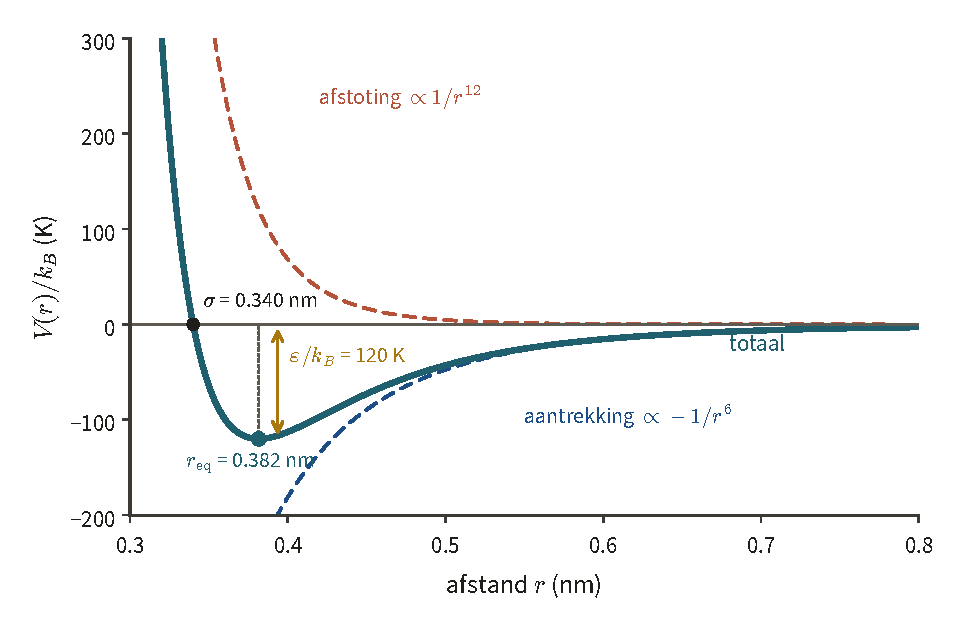
\includegraphics[width=0.7\linewidth]{Figuren/lennard_jones}
    \caption{De Lennard-Jones-potentiaal van argon ($\sigma=\SI{0.340}{\nano\metre}$, $\varepsilon/k_B=\SI{120}{\kelvin}$). De totale potentiaal (volle lijn) is de som van een steile afstoting $\propto 1/r^{12}$ en een zachtere aantrekking $\propto -1/r^6$ (stippellijnen). Het minimum ligt bij $r_{\text{eq}}=2^{1/6}\sigma$ en heeft diepte $\varepsilon$.}
    \label{fig:lennard-jones}
\end{figure}

\begin{voorbeeld}{Lennard-Jones-parameters voor argon}
\label{ex:argon-lj}
Voor argon geldt $\sigma = \SI{0.340}{\nano\metre}$ en $\varepsilon/k_B = \SI{120}{\kelvin}$ ($\varepsilon = \SI{1.65e-21}{\joule}$). De evenwichtsafstand bedraagt:
\[
r_{\text{eq}} = 2^{1/6} \cdot \SI{0.340}{\nano\metre} = \SI{0.382}{\nano\metre}.
\]
De bindingsenergie per mol bedraagt $N_A \varepsilon = \SI{994}{\joule\per\mole} \approx \SI{1.0}{\kilo\joule\per\mole}$. Dit is klein vergeleken met een covalente binding (\SI{400}{\kilo\joule\per\mole}), maar voldoende om argon bij \SI{87}{\kelvin} vloeibaar te maken. Het kookpunt blijkt inderdaad $\sim \varepsilon/k_B$, wat de fysische betekenis van de potentiaalkuil-diepte bevestigt. We gebruiken deze $\sigma$ en $\varepsilon$ verderop opnieuw (\S~\ref{sec:vdw-brug}) om de Van der Waals-parameter $a$ van argon te schatten.
\end{voorbeeld}

\section{De brug naar de vergelijking van Van der Waals}
\label{sec:vdw-brug}

In hoofdstuk~\ref{ch:eerstehoofdwet} introduceerden we de vergelijking van Van der Waals:
\begin{equation}
\left(p + \frac{a n^2}{V^2}\right)(V - nb) = nRT.
\end{equation}
De parameter $a$ corrigeert voor de intermoleculaire aantrekkingskrachten. Met behulp van de Lennard-Jones-potentiaal kan deze parameter fysisch worden ge\"interpreteerd en, in tegenstelling tot een louter evenredigheidsargument, ook effectief worden berekend.

Beschouw \'e\'en molecule, omringd door een gemiddelde, uniforme dichtheid van andere moleculen. Het aantal buurmoleculen in een dunne bolschil met straal $r$ en dikte $\dd{r}$ bedraagt $4\pi r^2\,\dd{r}$ maal de getalsdichtheid. De gemiddelde aantrekkingsenergie van \'e\'en molecule met al zijn buren wordt dan bekomen door de attractieve term van de Lennard-Jonespotentiaal, $V_{\text{attr}}(r) = -4\varepsilon(\sigma/r)^6$, te integreren over alle afstanden vanaf het punt waar de moleculen elkaar raken ($r=\sigma$) tot oneindig ver:
\begin{equation}
\overline{V}_{\text{attr}} = \int_{\sigma}^{\infty} 4\pi r^2\,V_{\text{attr}}(r)\,\dd{r} = -16\pi\varepsilon\sigma^6\int_{\sigma}^{\infty}\frac{\dd{r}}{r^4} = -16\pi\varepsilon\sigma^6\left[-\frac{1}{3r^3}\right]_{\sigma}^{\infty} = -\frac{16\pi}{3}\varepsilon\sigma^3.
\end{equation}
Omdat elk paar moleculen bij deze telling tweemaal wordt meegerekend (net zoals bij de afleiding van het co-volume $b$ in hoofdstuk~\ref{ch:eerstehoofdwet}, \S~\ref{sec:vdw-afleiding}), bedraagt de effectieve aantrekkingsenergie per mol de helft hiervan, vermenigvuldigd met het aantal Avogadro-paren:
\begin{equation}
\boxed{
a = -\frac{N_A^2}{2}\,\overline{V}_{\text{attr}} = \frac{8\pi}{3}N_A^2\,\varepsilon\sigma^3.
}
\label{eq:a-vdw-lj}
\end{equation}
De parameter $a$ is dus evenredig met het volume van de molecule ($\sigma^3$) en de diepte van de interactiekuil ($\varepsilon$), en vergelijking~\eqref{eq:a-vdw-lj} geeft bovendien de exacte evenredigheidsconstante binnen dit vereenvoudigde model. Hiermee krijgt de $a$-parameter uit hoofdstuk~\ref{ch:eerstehoofdwet} een microscopische fundering.

\begin{voorbeeld}{De Van der Waals-parameter $a$ van argon, geschat uit de Lennard-Jonespotentiaal}
Met de waarden $\sigma=\SI{0.340}{\nano\metre}$ en $\varepsilon=\SI{1.65e-21}{\joule}$ voor argon (voorbeeld~\ref{ex:argon-lj}) levert vergelijking~\eqref{eq:a-vdw-lj}:
\[
a = \frac{8\pi}{3}(6.022\times10^{23})^2(1.65\times10^{-21}\,\mathrm{J})(0.340\times10^{-9}\,\mathrm{m})^3 \approx \SI{0.197}{\pascal\,\metre^6\per\mole\squared}.
\]
De experimentele Van der Waals-parameter van argon bedraagt $a_{\text{Ar}}\approx\SI{0.1355}{\pascal\,\metre^6\per\mole\squared}$ (hoofdstuk~\ref{ch:eerstehoofdwet}, tabel met stofconstanten). Onze eenvoudige schatting zit dus binnen een factor anderhalf van de experimentele waarde --- een opmerkelijk goede overeenstemming voor een model dat de moleculaire dichtheid rond een molecule als uniform veronderstelt (dat wil zeggen: het verwaarloost dat buurmoleculen elkaar afschermen, wat in werkelijkheid door de paarcorrelatiefunctie $g(r)$ wordt beschreven). Dit bevestigt dat de Lennard-Jonesparameters $\varepsilon$ en $\sigma$, oorspronkelijk ingevoerd om spectroscopische en botsingsdata te beschrijven, en de macroscopische Van der Waals-parameter $a$, oorspronkelijk ingevoerd om afwijkingen van de ideale gaswet te beschrijven, twee kwantitatief consistente beschrijvingen zijn van dezelfde onderliggende intermoleculaire aantrekking.
\end{voorbeeld}

\section{Verdampingsenthalpie als maat voor cohesie}
\label{sec:verdampingsenthalpie}

De verdampingsenthalpie $\Delta H_{\text{vap}}$ van een zuivere vloeistof is de energie die nodig is om een molecule uit de vloeistoffase naar de gasfase te brengen, en dus om alle intermoleculaire interacties met zijn buren te verbreken. $\Delta H_{\text{vap}}$ is daarmee een directe experimentele maat voor de totale sterkte van de intermoleculaire krachten.

\begin{table}[h]
\centering
\begin{tabular}{lccc}
\toprule
Stof & $\Delta H_{\text{vap}}$ (\si{\kilo\joule\per\mole}) & $T_b$ & Dominante kracht \\
\midrule
He & 0{,}08 & \SI{4.2}{\kelvin} & Dispersie (zwak) \\
$\mathrm{N_2}$ & 5{,}6 & \SI{77.4}{\kelvin} & Dispersie \\
$\mathrm{CH_4}$ & 8{,}2 & \SI{111.7}{\kelvin} & Dispersie \\
$\mathrm{CHCl_3}$ & 29{,}4 & \SI{334.3}{\kelvin} & Dipool--dipool + dispersie \\
$\mathrm{NH_3}$ & 23{,}4 & \SI{239.8}{\kelvin} & Waterstofbrug (zwakker dan water) \\
$\mathrm{H_2O}$ & 40{,}7 & \SI{373.15}{\kelvin} & Waterstofbrug \\
Ethanol & 38{,}6 & \SI{351.55}{\kelvin} & Waterstofbrug \\
$\mathrm{NaCl}$ (sublimatie) & 211 & sublimeert & Ion--ion \\
\bottomrule
\end{tabular}
\caption{Verdampingsenthalpie\"en en normale kookpunten $T_b$ (bij \SI{1}{\bar}).}
\label{tab:verdampingsenthalpie}
\end{table}

De tabel toont duidelijk de hi\"erarchie: dispersie $<$ dipool--dipool $<$ waterstofbrug $<$ ion--ion. Zij beantwoordt bovendien meteen \'e\'en van de openingsvragen van dit hoofdstuk (\S~\ref{sec:voorbij-covalent}): methaan en stikstof, met een vergelijkbare molaire massa als water, bezitten enkel zwakke dispersiekrachten en koken daardoor al ver onder kamertemperatuur, terwijl water dankzij zijn waterstofbrugnetwerk pas bij \SI{373.15}{\kelvin} kookt. Voor de ingenieur is $\Delta H_{\text{vap}}$ een directe indicator voor het energieverbruik van een destillatieproces --- water en ethanol vereisen aanzienlijk meer energie dan koolwaterstoffen.

\subsection{De regel van Trouton}
\label{sec:trouton}

Tabel~\ref{tab:verdampingsenthalpie} bevat zowel $\Delta H_{\text{vap}}$ als het normale kookpunt $T_b$: de temperatuur waarbij, per definitie, de vloeistof- en dampfase bij \SI{1}{\bar} in evenwicht zijn. Uit hoofdstuk~\ref{ch:spontaniteit} (\S~\ref{sec:entropie-faseovergangen}) weten we dat voor elke reversibele faseovergang bij constante druk geldt $\Delta S_{\text{trans}}=\Delta H_{\text{trans}}/T_{\text{trans}}$. Toegepast op verdamping:
\begin{equation}
\Delta S_{\text{vap}} = \frac{\Delta H_{\text{vap}}}{T_b}.
\end{equation}
De empirische \emph{regel van Trouton} stelt dat deze verdampingsentropie voor de meeste ``normale'' vloeistoffen --- dat wil zeggen vloeistoffen zonder sterke, gerichte intermoleculaire interacties zoals waterstofbruggen --- ongeveer dezelfde waarde aanneemt, typisch $\Delta S_{\text{vap}}\approx\SIrange{85}{88}{\joule\per\mole\per\kelvin}$. De fysische reden is intuïtief: bij het koken wint elke vloeistof, ongeacht haar chemische aard, ongeveer dezelfde \emph{relatieve} toename in bewegingsvrijheid (van een gecondenseerde naar een verdunde gasfase), zodat de toename in het aantal toegankelijke microtoestanden (\S~\ref{sec:waarschijnlijkheid-entropie} in hoofdstuk~\ref{ch:spontaniteit}) voor de meeste vloeistoffen vergelijkbaar is.

\begin{voorbeeld}{Trouton's regel getoetst aan tabel~\ref{tab:verdampingsenthalpie}}
We berekenen $\Delta S_{\text{vap}}=\Delta H_{\text{vap}}/T_b$ voor elke stof uit tabel~\ref{tab:verdampingsenthalpie}:
\begin{center}
\begin{tabular}{lc}
\toprule
Stof & $\Delta S_{\text{vap}}$ (\si{\joule\per\mole\per\kelvin}) \\
\midrule
$\mathrm{N_2}$ (dispersie) & $5600/77.4 = 72.4$ \\
$\mathrm{CH_4}$ (dispersie) & $8200/111.7 = 73.4$ \\
$\mathrm{CHCl_3}$ (dipool--dipool) & $29400/334.3 = 87.9$ \\
$\mathrm{NH_3}$ (zwakke waterstofbrug) & $23400/239.8 = 97.6$ \\
$\mathrm{H_2O}$ (waterstofbrug) & $40700/373.15 = 109.1$ \\
Ethanol (waterstofbrug) & $38600/351.55 = 109.8$ \\
\bottomrule
\end{tabular}
\end{center}
Het patroon is opmerkelijk consistent: chloroform, dat enkel dipool--dipool- en dispersiekrachten bezit, voldoet vrijwel exact aan de regel van Trouton ($\approx\SI{88}{\joule\per\mole\per\kelvin}$). Stikstof en methaan liggen er iets onder (een bekende afwijking voor kleine, quasi-boldeeltjes met weinig interne vrijheidsgraden, zie hoofdstuk~\ref{ch:kwantum}, \S~\ref{sec:moleculaire-beweging}). Ammoniak, water en ethanol wijken daarentegen sterk en systematisch \emph{naar boven} af: hun waterstofbrugnetwerk (\S~\ref{sec:waterstofbruggen}) moet bij het verdampen worden opgebroken, wat een extra, geordend-naar-ongeordend effect toevoegt bovenop de gewone toename in bewegingsvrijheid. Merk op dat de waarde voor water, $\SI{109.1}{\joule\per\mole\per\kelvin}$, overeenkomt met de waarde $\Delta S_{\text{vap}}\approx\SI{109}{\joule\per\mole\per\kelvin}$ die reeds in hoofdstuk~\ref{ch:spontaniteit} werd berekend. Trouton's regel levert een ingenieur zo een snelle, eerste-orde consistentiecontrole: een sterke afwijking van $\approx\SI{85}{\joule\per\mole\per\kelvin}$ is een directe indicatie van gerichte intermoleculaire interacties (waterstofbruggen) die in een proces- of destillatieontwerp niet over het hoofd mogen worden gezien.
\end{voorbeeld}

\section{Mengsels: regelmatige oplossingen en de Hildebrand-parameter}

Wanneer twee vloeistoffen mengen, worden intermoleculaire interacties verbroken en nieuwe gevormd. De mengenthalpie is de nettobalans hiervan. Voor \emph{regelmatige oplossingen} (geen waterstofbruggen, geen sterke dipoolinteracties) ontwikkelde Hildebrand een kwantitatieve theorie.

\subsection{De Hildebrand-oplosbaarheidsparameter}
\label{sec:hildebrand}

De \emph{Hildebrand-parameter} $\delta$ is gedefinieerd als:
\begin{equation}
\boxed{\;\delta = \sqrt{\frac{\Delta E_{\text{vap}}}{V_m}}\;}
\end{equation}
waarin $\Delta E_{\text{vap}} = \Delta H_{\text{vap}} - RT$ de molaire verdampingsenergie (energie, niet enthalpie) en $V_m$ het molaire volume zijn. De eenheid is \si{\joule\per\centi\metre\cubed} of equivalent \si{\mega\pascal^{1/2}}.

De mengenthalpie voor twee vloeistoffen met gelijke volumes wordt benaderd door:
\begin{equation}
\Delta H_{\text{meng}} \approx V\,(\delta_1 - \delta_2)^2\,\phi_1\,\phi_2,
\end{equation}
waarin $\phi_i$ de volumefracties zijn. \emph{Gelijksoortige $\delta$-waarden leiden tot mengbaarheid}; sterk verschillende waarden leiden tot demixing --- via het spontaniteitscriterium $\Delta G_{\text{meng}}=\Delta H_{\text{meng}}-T\Delta S_{\text{meng}}$ uit hoofdstuk~\ref{ch:spontaniteit}: wanneer $\Delta H_{\text{meng}}$ voldoende groot en positief is, kan het de (steeds positieve, maar begrensde) mengentropiebijdrage $-T\Delta S_{\text{meng}}$ overtreffen, zodat $\Delta G_{\text{meng}}>0$ en de vloeistoffen zich spontaan ontmengen.

\begin{voorbeeld}{Water en hexaan}
De Hildebrand-parameters bedragen:
\begin{itemize}
\item Water: $\delta = \SI{47.9}{\mega\pascal^{1/2}}$ (sterk waterstofbruggend)
\item $n$-Hexaan: $\delta = \SI{14.9}{\mega\pascal^{1/2}}$ (niet-polair koolwaterstof)
\end{itemize}
Het verschil is groot, waardoor $\Delta H_{\text{meng}}$ zeer positief is. De Gibbs-energie van mengen (hoofdstuk~\ref{ch:niet-reagerend}, \S~\ref{sec:thermodynamica-mengsels}) wordt dan positief, en de vloeistoffen mengen niet. Dit verklaart, kwantitatief, waarom olie en water zich splitsen --- exact de vraag die in \S~\ref{sec:voorbij-covalent} werd gesteld.

Voor twee koolwaterstoffen, bv. hexaan ($\delta = \SI{14.9}{\mega\pascal^{1/2}}$) en heptaan ($\delta = \SI{15.2}{\mega\pascal^{1/2}}$), is het verschil klein en mengen de vloeistoffen volledig. In de chromatografie en de verfindustrie wordt de Hildebrand-parameter gebruikt om compatibele oplosmiddelen te selecteren.
\end{voorbeeld}

\subsection{Beperkingen}

De Hildebrand-theorie werkt goed voor niet-polaire of zwak polaire mengsels zonder specifieke interacties. Voor systemen met waterstofbruggen (water, alcoholen) of sterke dipoolinteracties bestaat geen enkelvoudige theorie die zonder meer bruikbaar is; de Hansen-parameters, die $\delta$ opsplitsen in dispersie-, dipool- en waterstofbrug-bijdragen, bieden een verbetering.

\section{Sterkte en reikwijdte}
\label{sec:sterkte-reikwijdte}

Een belangrijk onderscheid tussen de intermoleculaire krachten is hun \emph{reikwijdte}:

\begin{itemize}
\item \textbf{Ion--ion}: $V \propto 1/r$ --- lange reikwijdte, orde van meerdere nanometer.
\item \textbf{Ion--dipool}: $V \propto 1/r^4$ --- matige reikwijdte.
\item \textbf{Van der Waals} (Keesom, Debye, London): $V \propto 1/r^6$ --- korte reikwijdte, enkel significant binnen \SI{1}{\nano\metre}.
\item \textbf{Waterstofbrug}: sterk gericht, typisch \SIrange{0.18}{0.25}{\nano\metre}.
\end{itemize}

\begin{figure}[htb]
    \centering
    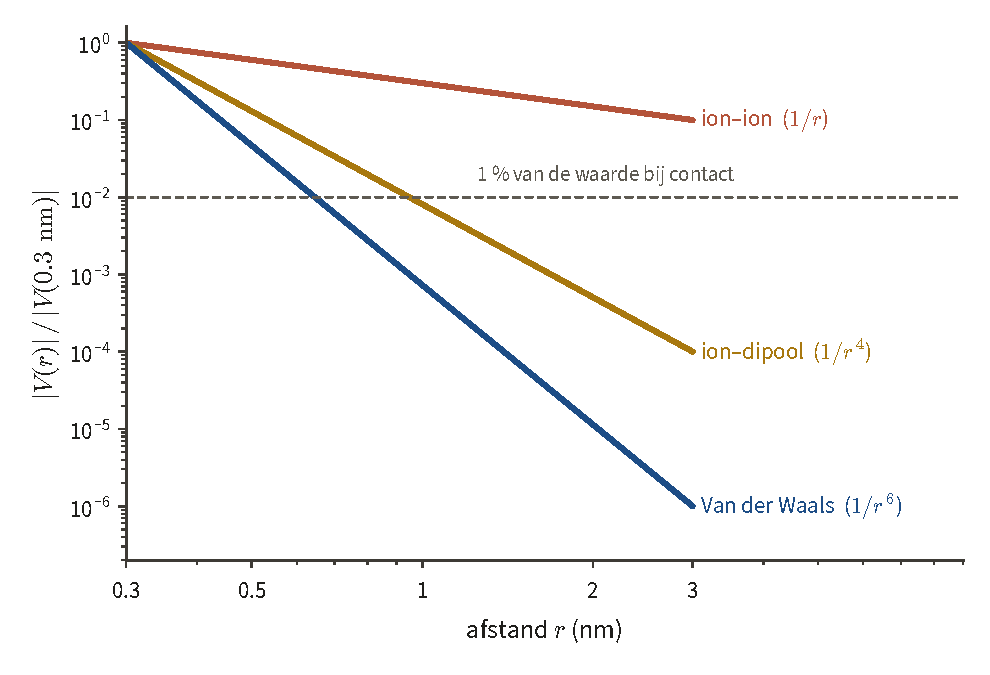
\includegraphics[width=0.7\linewidth]{Figuren/reikwijdte}
    \caption{Relatieve sterkte van de interactie-energie $|V(r)|$ als functie van de afstand, op een logaritmische schaal en genormaliseerd op $r = \SI{0.3}{\nano\metre}$. De Coulombinteractie tussen ionen ($1/r$) reikt veel verder dan de ion--dipoolinteractie ($1/r^4$) en de Van der Waalskrachten ($1/r^6$). Bij een verdubbeling van de afstand daalt een Van der Waalsinteractie met een factor 64.}
    \label{fig:reikwijdte}
\end{figure}

Dit onderscheid is belangrijk voor de collo\"idchemie (hoofdstuk~\ref{ch:oppervlakte}): bij de DLVO-theorie worden lange-reikwijdte elektrostatische afstoting (van geladen oppervlakken) vergeleken met korte-reikwijdte Van der Waals-aantrekking.

\section{Kwantitatieve vergelijking van de krachten}

De volgende tabel geeft een orde-grootte-overzicht van alle behandelde interacties:

\begin{table}[h]
\centering
\begin{tabular}{lcc}
\toprule
Type & Energie (\si{\kilo\joule\per\mole}) & Afhankelijkheid \\
\midrule
Covalente binding & 200--800 & Complex \\
Ion--ion & 200--800 & $1/r$ \\
Ion--dipool & 40--600 & $1/r^4$, $1/T$ \\
Waterstofbrug & 10--40 & Gericht, \SI{0.2}{\nano\metre} \\
Dipool--dipool (Keesom) & 5--25 & $1/r^6$, $1/T$ \\
Dipool--ge\"ind. (Debye) & 2--10 & $1/r^6$ \\
Dispersie (London) & 0{,}5--10 & $1/r^6$ \\
\bottomrule
\end{tabular}
\caption{Ordes van grootte van intermoleculaire krachten.}
\end{table}

Een opvallende observatie: alle Van der Waalskrachten (Keesom, Debye, London) delen dezelfde $1/r^6$-afhankelijkheid. Dit is geen toeval: alle drie zijn ze zwakke storingen van de elektronenstructuur, en dezelfde wiskundige structuur geldt. Merk verder op dat de energiebereiken van de covalente binding en de ion--ioninteractie elkaar volledig overlappen: het onderscheid tussen ``intramoleculair'' en ``intermoleculair'' is dus niet in de eerste plaats een kwestie van energieschaal, maar van de aard van de interactie (gedeelde elektronenparen versus elektrostatische aantrekking tussen afgeronde ladingen, hoofdstuk~\ref{ch:kwantum}).

\section{Intermoleculaire krachten aan het werk}
\label{sec:im-toepassingen}

Intermoleculaire krachten zijn zwak in vergelijking met chemische bindingen, maar ze werken overal en altijd. In deze paragraaf bekijken we een reeks situaties uit het dagelijks leven en de industrie waarin ze de doorslag geven. Telkens stellen we dezelfde vraag: \emph{welke kracht domineert, en wat volgt daaruit?}

\begin{toepassing}{Water koken: veel energie, en soms een verrassing}
Om water te verdampen moeten alle waterstofbruggen van een molecule met zijn buren verbroken worden. Daarom is de verdampingsenthalpie van water per kilogram uitzonderlijk hoog: \SI{2257}{\kilo\joule\per\kilo\gram}, tegenover \SI{838}{} voor ethanol en \SI{335}{\kilo\joule\per\kilo\gram} voor hexaan. Dat maakt stoom de ideale warmtedrager in de industrie: een kilogram condenserende stoom levert veel warmte bij een constante temperatuur. Om dezelfde reden is een koeltoren zo effici\"ent: verdampt \SI{1}{\percent} van het koelwater, dan koelt de rest ongeveer \SI{5}{\kelvin} af.

De sterke cohesie heeft ook een keerzijde. Een dampbel kan pas groeien als ze groot genoeg is om de oppervlaktespanning te overwinnen. In een zeer gladde, schone kom (bv.\ een glas water in de microgolfoven) ontbreken de kleine oneffenheden of luchtbelletjes waarop bellen kunnen ontstaan. Het water kan dan enkele graden boven \SI{100}{\celsius} komen zonder te koken, en bij de minste verstoring explosief opkoken. In het labo voorkom je dat met kookstenen; in een verdamper met een ruw oppervlak of een kleine gasstroom.
\end{toepassing}

\begin{toepassing}{Lijmen en kleefband: contact is alles}
Een lijm of een kleefband hecht vooral via Van der Waalskrachten en, als de oppervlakken polair zijn, via waterstofbruggen. Hoe sterk kan dat zijn? Voor twee vlakke oppervlakken op afstand $D$ geeft de theorie een aantrekking per oppervlakte
\begin{equation}
\frac{F}{A} = \frac{A_\mathrm{H}}{6\pi D^3},
\label{eq:hamaker}
\end{equation}
met $A_\mathrm{H} \approx \SI{1e-19}{\joule}$ de \emph{Hamakerconstante}. Bij moleculair contact ($D \approx \SI{0.4}{\nano\metre}$) is dat
\[
\frac{F}{A} = \frac{10^{-19}}{6\pi(0.4\times10^{-9})^3} \approx \SI{8e7}{\pascal} = \SI{800}{\bar}.
\]
Twee perfect vlakke oppervlakken zouden dus enorm sterk aan elkaar kleven. In de praktijk raken twee vaste stoffen elkaar maar op enkele toppen van hun ruwheid; elders is $D$ honderden keren groter, en door de $1/D^3$-afhankelijkheid valt de kracht weg. Daarom is een lijm altijd \emph{vloeibaar} wanneer hij wordt aangebracht: hij vloeit in alle oneffenheden en maakt zo overal moleculair contact. Pas daarna hardt hij uit.

De gekko gebruikt hetzelfde principe zonder lijm. Zijn tenen dragen miljoenen fijne haartjes die zich elk afzonderlijk aan de ruwheid van een muur aanpassen. De gemeten hechting, ongeveer \SI{10}{\newton\per\square\centi\metre}, is duizendmaal minder dan de theoretische waarde, maar ruim voldoende om het dier aan \'e\'en poot te laten hangen.

Waarom kleeft bijna niets aan polyetheen of teflon? Hun oppervlak heeft enkel zwakke dispersiekrachten en geen polaire groepen (lage \emph{oppervlakte-energie}: \SI{20}{} tot \SI{33}{\milli\joule\per\square\metre}, tegenover \SI{72}{} voor water en ruim boven \SI{100}{} voor glas of metaal). Een lijm bevochtigt zo'n oppervlak slecht. Industrieel behandelt men kunststof daarom eerst met een corona- of plasmabehandeling, die polaire groepen (\ce{-OH}, \ce{-COOH}) op het oppervlak aanbrengt.
\end{toepassing}

\begin{toepassing}{Coatings: waterafstotend, krasvast of vuilafstotend}
Een coating moet aan de ondergrond hechten, maar haar buitenkant moet vaak net \emph{niet} kleven. Een waterafstotende coating (teflon, siliconen, fluorhoudende impregneermiddelen voor textiel) heeft aan de buitenkant enkel \ce{-CF3}- of \ce{-CH3}-groepen. Water vormt er geen waterstofbruggen mee en trekt zich samen tot druppels. Fluor is daarbij bijzonder effectief: het is klein en zeer weinig polariseerbaar, zodat zelfs de dispersiekrachten zwak zijn.

Bij het formuleren van een verf kies je het oplosmiddel met de Hildebrandparameter uit \S~\ref{sec:hildebrand}: het oplosmiddel moet het bindmiddel (de polymeerhars) goed oplossen, dus een vergelijkbare $\delta$ hebben, en daarna snel genoeg verdampen. Dezelfde redenering verklaart waarom aceton een verflaag of piepschuim aantast, en water niet.
\end{toepassing}

\begin{toepassing}{Adsorptie: moleculen vasthouden op een oppervlak}
Actieve kool heeft een inwendig oppervlak van \SIrange{500}{1500}{\square\metre\per\gram}: \'e\'en theelepel heeft het oppervlak van een voetbalveld. Organische moleculen blijven er via dispersiekrachten aan hangen (\emph{fysisorptie}, typisch \SIrange{5}{40}{\kilo\joule\per\mole}). Grote, goed polariseerbare moleculen (oplosmiddeldampen, geurstoffen, chloor uit leidingwater) worden het sterkst vastgehouden; kleine, weinig polariseerbare gassen zoals \ce{N2} en \ce{O2} nauwelijks. Daarom werkt een actief-koolfilter in een dampkap of een gasmasker.

Zeolieten zijn kristallijne alumino-silicaten met pori\"en van moleculaire afmetingen en geladen kationen (\ce{Na+}, \ce{Ca^2+}) in hun wanden. Watermoleculen binden er via ion--dipoolinteracties, met een adsorptie-enthalpie die hoger ligt dan de condensatie-enthalpie van water. Zeolieten drogen gassen en oplosmiddelen daardoor tot extreem lage watergehaltes. Zuurstofconcentratoren gebruiken een zeoliet die \ce{N2} sterker bindt dan \ce{O2}: het quadrupoolmoment van \ce{N2} is groter en interageert met de kationen. Adsorptie komt uitgebreid terug in hoofdstuk~\ref{ch:oppervlakte}.
\end{toepassing}

\begin{toepassing}{Nylon versus polyetheen}
Polyetheen (PE) en nylon-6,6 zijn beide lange ketens, maar hun eigenschappen verschillen sterk. Tussen PE-ketens werken enkel dispersiekrachten; HDPE smelt rond \SI{130}{\celsius}. In nylon vormen de amidegroepen (\ce{-CO-NH-}) waterstofbruggen tussen naburige ketens; nylon-6,6 smelt pas bij \SI{265}{\celsius}, is stijver en sterker. Kevlar gaat nog verder: zijn starre ketens liggen perfect geordend naast elkaar met een waterstofbrug om de paar atomen. Per gewicht is een Kevlarvezel vijf keer sterker dan staal.

De keerzijde: dezelfde amidegroepen trekken water aan. Nylon neemt enkele procent vocht op, zwelt en wordt zachter. Bij het spuitgieten moet nylongranulaat daarom eerst gedroogd worden.
\end{toepassing}

\begin{toepassing}{Smeermiddelen}
Een smeerolie bestaat uit lange koolwaterstofketens. De dispersiekrachten tussen de ketens bepalen de viscositeit: langere ketens geven meer contactpunten en een dikkere olie. Bij hogere temperatuur bewegen de ketens sneller en daalt de viscositeit sterk; additieven (lange polymeren die bij hoge temperatuur ontrollen) beperken dat effect. Vaste smeermiddelen zoals grafiet en \ce{MoS2} hebben een gelaagde structuur: binnen een laag sterke covalente bindingen, tussen de lagen enkel zwakke Van der Waalskrachten. De lagen schuiven daardoor gemakkelijk over elkaar.
\end{toepassing}

\begin{toepassing}{Koelmiddelen en luchtscheiding}
Een koelmiddel moet verdampen bij een lage temperatuur (zwakke intermoleculaire krachten) en daarbij toch veel warmte opnemen (voldoende sterke krachten). Ammoniak, met waterstofbruggen, kookt bij \SI{-33}{\celsius} en neemt \SI{1370}{\kilo\joule\per\kilo\gram} op; het fluorhoudende R-134a kookt bij \SI{-26}{\celsius} maar neemt slechts \SI{217}{\kilo\joule\per\kilo\gram} op. Ammoniak is daarom het koelmiddel van grote industri\"ele installaties (koelhuizen, brouwerijen), ondanks zijn giftigheid.

Bij de cryogene luchtscheiding worden stikstof (kookpunt \SI{77.4}{\kelvin}), argon (\SI{87.3}{\kelvin}) en zuurstof (\SI{90.2}{\kelvin}) door destillatie gescheiden. Deze moleculen hebben enkel dispersiekrachten van vergelijkbare sterkte; de kookpunten liggen daardoor dicht bij elkaar en de kolommen zijn hoog, met tientallen schotels.
\end{toepassing}

\begin{toepassing}{DNA en geneesmiddelen}
De twee strengen van DNA worden samengehouden door waterstofbruggen tussen de basen: twee tussen A en T, drie tussen G en C. Elke brug is zwak, maar met duizenden achter elkaar is de dubbele helix stabiel. Bij verhitting tot ongeveer \SI{95}{\celsius} breken ze en gaan de strengen uit elkaar; de PCR-techniek benut dat. Een geneesmiddel werkt op dezelfde manier: het past in de holte van een eiwit en wordt daar vastgehouden door een combinatie van waterstofbruggen, ionische interacties en dispersiekrachten. Een kleine wijziging van \'e\'en groep kan de binding honderd keer sterker of zwakker maken.
\end{toepassing}

\section{Samenvatting en reflectie}

\begin{samenvatting}{Intermoleculaire krachten}
\begin{itemize}
\item Intermoleculaire krachten zijn van elektrostatische oorsprong. Van sterk naar zwak: ion--ion, ion--dipool, waterstofbrug, dipool--dipool (Keesom), dipool--ge\"induceerde dipool (Debye) en dispersie (London).
\item Dispersiekrachten werken tussen alle moleculen en groeien met de polariseerbaarheid, dus met de grootte van de elektronenwolk. Bij grote moleculen domineren ze vaak.
\item De Lennard-Jonespotentiaal combineert afstoting ($1/r^{12}$) en aantrekking ($1/r^6$); de parameters $\varepsilon$ en $\sigma$ hangen samen met de Van der Waalsconstanten $a$ en $b$.
\item De verdampingsenthalpie is een maat voor de cohesie. Volgens de regel van Trouton is $\Delta S_\mathrm{vap} \approx \SI{85}{\joule\per\mole\per\kelvin}$; vloeistoffen met waterstofbruggen wijken naar boven af.
\item De Hildebrandparameter $\delta = \sqrt{\Delta E_\mathrm{vap}/V_\mathrm{m}}$ voorspelt de mengbaarheid: gelijkaardige $\delta$ mengt.
\item Toepassingen: koken en stoom als warmtedrager, lijmen (contact is alles, $F/A \propto 1/D^3$), coatings, adsorptie, polymeren, smeermiddelen, koelmiddelen en biomoleculen.
\end{itemize}
\end{samenvatting}

\begin{reflectie}{Intermoleculaire krachten}
\begin{enumerate}
\item Methaan en water hebben bijna dezelfde molaire massa. Waarom is het ene een gas en het andere een vloeistof bij kamertemperatuur?
\item Waarom stijgt het kookpunt van de alkanen met de ketenlengte, terwijl de moleculen niet polair zijn?
\item Een lijm hecht goed op glas, maar niet op een plastic boterpot. Verklaar, en geef een industri\"ele oplossing.
\item Waarom moet een lijm vloeibaar zijn wanneer je hem aanbrengt?
\item Waarom houdt actieve kool tolueendamp goed vast en stikstof nauwelijks?
\item Nylon en polyetheen zijn beide lange polymeerketens. Waarom smelt nylon bij een veel hogere temperatuur, en waarom moet het gedroogd worden voor verwerking?
\item Welke eigenschappen zoek je in een goed koelmiddel, en hoe hangen die samen met de intermoleculaire krachten?
\end{enumerate}
\end{reflectie}

Intermoleculaire krachten blijven in de volgende hoofdstukken op de achtergrond aanwezig: in de afwijkingen van de wet van Raoult en de activiteitsco\"effici\"enten (hoofdstuk~\ref{ch:niet-reagerend}) en in de adsorptie en oppervlaktespanning (hoofdstuk~\ref{ch:oppervlakte}).

\newpage
\section{Oefeningen}

% Oefeningen bij dit hoofdstuk (ingevoegd achteraan het hoofdstuk met \input).
% Een oefening:  \begin{oefening}[titel] ... \end{oefening}   (boek en website)
% De oplossing:  \begin{oplossing} ... \end{oplossing}       (enkel website, dichtgeklapt)

Constanten: $R = \SI{8.314}{\joule\per\mole\per\kelvin}$, $k_B = \SI{1.381e-23}{\joule\per\kelvin}$, $N_A = \SI{6.022e23}{\per\mole}$, $4\pi\varepsilon_0 = \SI{1.113e-10}{\coulomb\squared\per\joule\per\metre}$.

\begin{oefening}[Kookpunten van een homologe reeks]
De kookpunten van de \(n\)-alkanen bij \(1\,\mathrm{bar}\) zijn:

\begin{center}
\begin{tabular}{lllllll}
\toprule
Alkaan & \(\mathrm{CH_4}\) & \(\mathrm{C_2H_6}\) & \(\mathrm{C_3H_8}\) & \(\mathrm{C_4H_{10}}\) & \(\mathrm{C_5H_{12}}\) & \(\mathrm{C_6H_{14}}\) \\
\midrule
\(T_b\) (°C) & \(-162\) & \(-89\) & \(-42\) & \(0\) & \(36\) & \(69\) \\
\bottomrule
\end{tabular}
\end{center}

\begin{enumerate}
\item[(a)]
  Verklaar de trend vanuit intermoleculaire krachten. Welke kracht is dominant?
\item[(b)]
  Waarom stijgt het kookpunt minder snel naarmate de keten langer wordt?
\item[(c)]
  Voorspel het kookpunt van \(n\)-octaan (\(\mathrm{C_8H_{18}}\)).
\end{enumerate}
\end{oefening}
\begin{oplossing}
\textbf{Resultaat:} (a) \textbf{London-dispersie}. (c) \(T_b\)(octaan) \ensuremath{\approx{}} \textbf{125 °C} (experimenteel 126 °C).

\textbf{(a)} Alkanen zijn apolair: enkel London-dispersie werkt. Elke extra \(\mathrm{CH_2}\)-groep voegt elektronen toe, waardoor de polariseerbaarheid en het contactoppervlak tussen de ketens toenemen. De dispersie-energie per molecule stijgt en er is meer warmte nodig om de moleculen uit de vloeistof te halen.

\textbf{(b)} Elke \(\mathrm{CH_2}\)-groep voegt een ongeveer constant bedrag toe aan \(\Delta H_{\text{vap}}\) (ongeveer \(4\)--\(5\,\mathrm{kJ/mol}\)). Volgens Trouton is \(T_b \approx \Delta H_{\text{vap}}/\Delta S_{\text{vap}}\); in absolute temperatuur is een zelfde stijging van \(\Delta H_{\text{vap}}\) relatief steeds kleiner. Bovendien kunnen lange ketens opkrullen, waardoor niet elke extra groep volledig in contact komt met de buren.

\textbf{(c)} De stijging per koolstofatoom daalt van \(73\) naar \(33\,^\circ\mathrm{C}\); extrapolatie (ongeveer \(+30\) en \(+28\,^\circ\mathrm{C}\) voor \(\mathrm{C_7}\) en \(\mathrm{C_8}\)) geeft \(T_b \approx 125\,^\circ\mathrm{C}\). De experimentele waarde is \(126\,^\circ\mathrm{C}\). Dit is precies waarom men ruwe olie in een destillatiekolom kan scheiden in fracties: gas, benzine, kerosine, diesel.
\end{oplossing}

\begin{oefening}[Waterstofbruggen: vergelijking van \(\mathrm{H_2O}\), \(\mathrm{H_2S}\), \(\mathrm{H_2Se}\) en \(\mathrm{H_2Te}\)]
De kookpunten van de waterstofverbindingen van groep 16 zijn: \(\mathrm{H_2O}\) \(100\,^\circ\mathrm{C}\), \(\mathrm{H_2S}\) \(-60\,^\circ\mathrm{C}\), \(\mathrm{H_2Se}\) \(-42\,^\circ\mathrm{C}\) en \(\mathrm{H_2Te}\) \(-2\,^\circ\mathrm{C}\). De verdampingsenthalpieën van \(\mathrm{H_2O}\) en \(\mathrm{H_2S}\) bedragen \(40.7\) en \(18.7\,\mathrm{kJ/mol}\).

\begin{enumerate}
\item[(a)]
  Verklaar waarom het kookpunt stijgt van \(\mathrm{H_2S}\) naar \(\mathrm{H_2Te}\), maar \(\mathrm{H_2O}\) een anomalie vormt.
\item[(b)]
  Hoeveel waterstofbruggen kan een watermolecule gemiddeld vormen? Verklaar het netwerkkarakter.
\item[(c)]
  Bereken de verhouding \(\Delta H_{\text{vap}}(\mathrm{H_2O})/\Delta H_{\text{vap}}(\mathrm{H_2S})\). Verklaar de verhouding vanuit de aard van de intermoleculaire krachten.
\end{enumerate}
\end{oefening}
\begin{oplossing}
\textbf{Resultaat:} (a) \textbf{Waterstofbruggen} in water. (b) Tot \textbf{vier} waterstofbruggen per molecule. (c) Verhouding \textbf{2.2}.

\textbf{(a)} Van S naar Te worden de moleculen groter en beter polariseerbaar: London-dispersie neemt toe, en daarmee het kookpunt. Zonder waterstofbruggen zou water, volgens deze trend, rond \(-80\,^\circ\mathrm{C}\) koken. Zuurstof is echter klein en sterk elektronegatief: de O--H binding is sterk gepolariseerd en de vrije elektronenparen op O zijn goed toegankelijk, zodat water sterke waterstofbruggen vormt. S, Se en Te zijn te weinig elektronegatief.

\textbf{(b)} Elke watermolecule heeft twee H-atomen (donoren) en twee vrije elektronenparen (acceptoren) en kan dus tot vier waterstofbruggen vormen, tetraëdrisch georiënteerd. In vloeibaar water zijn er gemiddeld ongeveer 3.5 per molecule. Dat geeft een driedimensionaal netwerk dat voortdurend breekt en opnieuw gevormd wordt (op een tijdschaal van picoseconden). In ijs is het netwerk volledig en open, wat verklaart waarom ijs drijft.

\textbf{(c)} \(40.7/18.7 = 2.2\). In \(\mathrm{H_2S}\) werken enkel dipool--dipool- en dispersiekrachten; in water komt het waterstofbrugnetwerk daarbovenop, dat meer dan de helft van de cohesie levert. Dit verklaart waarom water zo'n uitstekend koelmiddel en warmtebuffer is (hoofdstuk 1), maar ook waarom het indampen van waterige stromen in de industrie zoveel energie kost.
\end{oplossing}

\begin{oefening}[Lennard-Jones: parameters en verdampingsenthalpie]
Voor methaan gelden \(\sigma = 0.381\,\mathrm{nm}\) en \(\varepsilon/k_B = 148\,\mathrm{K}\).

\begin{enumerate}
\item[(a)]
  Bereken de evenwichtsafstand \(r_{\text{eq}}\).
\item[(b)]
  Bereken de molaire interactie-energie \(N_A\varepsilon\) van één paar.
\item[(c)]
  Vergelijk met de experimentele verdampingsenthalpie \(\Delta H_{\text{vap}} = 8.2\,\mathrm{kJ/mol}\). Verklaar de verhouding (een molecule heeft ongeveer 12 buren in de vloeistof).
\end{enumerate}
\end{oefening}
\begin{oplossing}
\textbf{Resultaat:} (a) \(r_{\text{eq}}\) = \textbf{0.428 nm}. (b) \(N_A\varepsilon\) = \textbf{1.23 kJ/mol}. (c) Verhouding \textbf{6.7} \ensuremath{\approx{}} 6 paarinteracties per molecule.

\textbf{(a)} \(r_{\text{eq}} = 2^{1/6}\sigma = 1.122 \times 0.381 = 0.428\,\mathrm{nm}\).

\textbf{(b)} \(N_A\varepsilon = N_A k_B (148\,\mathrm{K}) = R(148) = 1.23\,\mathrm{kJ/mol}\).

\textbf{(c)} \(8.2/1.23 = 6.7\). Bij verdamping verbreekt een molecule ongeveer 12 contacten met buren, maar elk contact wordt gedeeld door twee moleculen: per molecule verdwijnen dus ongeveer \(12/2 = 6\) paarinteracties. De verwachte verdampingsenergie is \(6 N_A\varepsilon \approx 7.4\,\mathrm{kJ/mol}\), en met \(\Delta H = \Delta U + RT\) (bij \(112\,\mathrm{K}\) ongeveer \(0.9\,\mathrm{kJ/mol}\)) komt men op \(8.3\,\mathrm{kJ/mol}\): een opmerkelijke overeenkomst voor zo'n eenvoudig model.
\end{oplossing}

\begin{oefening}[Hildebrand-parameter en mengbaarheid]
Gegeven de Hildebrand-parameters: tolueen \(\delta = 18.2\,\mathrm{MPa^{1/2}}\), cyclohexaan \(16.8\), methanol \(29.7\) en water \(47.9\,\mathrm{MPa^{1/2}}\). De molaire volumes van tolueen en methanol zijn \(106.8\) en \(40.5\,\mathrm{cm^3/mol}\).

\begin{enumerate}
\item[(a)]
  Welke paren vloeistoffen zullen volgens de Hildebrand-theorie volledig mengen? Welke niet?
\item[(b)]
  Bereken de mengenthalpie per liter voor een 50/50-mengsel (volumefracties) van tolueen en methanol. Vergelijk met de bijdrage \(T\Delta S_{\text{meng}}\) van een ideaal mengsel bij \(298\,\mathrm{K}\). Wat voorspelt de theorie?
\item[(c)]
  In werkelijkheid mengen tolueen en methanol volledig, en ook methanol en water. Waarom faalt de Hildebrand-parameter hier?
\end{enumerate}
\end{oefening}
\begin{oplossing}
\textbf{Resultaat:} (a) Enkel \textbf{tolueen--cyclohexaan} mengt volgens de theorie. (b) \(\Delta H_{\text{meng}}\) = \textbf{33 kJ} \textgreater{} \(T\Delta S\) = 25 kJ: theorie voorspelt ontmenging. (c) Waterstofbruggen vallen buiten het model.

\textbf{(a)} Kleine \(\Delta\delta\) betekent mengbaar. Tolueen--cyclohexaan (\(\Delta\delta = 1.4\)) mengt volledig. Volgens de theorie zouden tolueen--methanol (\(11.5\)), methanol--water (\(18.2\)) en zeker tolueen--water (\(29.7\)) en cyclohexaan--water niet mengen.

\textbf{(b)} Met \((\Delta\delta)^2 = (11.5)^2 = 132\,\mathrm{MPa} = 1.32\times10^{8}\,\mathrm{J/m^3}\):

\[
\Delta H_{\text{meng}} = V(\delta_1 - \delta_2)^2\phi_1\phi_2 = (10^{-3})(1.32\times10^{8})(0.5)(0.5) = 33\,\mathrm{kJ}\ \text{per liter}
\]

Eén liter bevat \(4.68\,\mathrm{mol}\) tolueen en \(12.35\,\mathrm{mol}\) methanol (\(x_{\text{tol}} = 0.275\)), dus \(\Delta S_{\text{meng}} = -R\sum n_i\ln x_i = 83\,\mathrm{J/K}\) en \(T\Delta S_{\text{meng}} = 25\,\mathrm{kJ}\). Omdat \(\Delta H_{\text{meng}} > T\Delta S_{\text{meng}}\), voorspelt de theorie \(\Delta G_{\text{meng}} > 0\): ontmenging.

\textbf{(c)} De Hildebrand-theorie geldt voor regelmatige oplossingen zonder specifieke interacties. Methanol en water vormen onderling waterstofbruggen die even sterk zijn als die in de zuivere stoffen; de theorie, die enkel naar de totale cohesie kijkt, ziet dat niet. Ook tolueen kan als zwakke acceptor (\ensuremath{\pi{}}-elektronen) met de OH-groep van methanol interageren. Voor zulke systemen gebruikt men Hansen-parameters, die \(\delta\) opsplitsen in dispersie-, polaire en waterstofbrugbijdragen, of activiteitscoëfficiëntmodellen (hoofdstuk 5).
\end{oplossing}

\begin{oefening}[Brug naar Van der Waals: van \(\varepsilon\) naar \(a\)]
De Van der Waals-parameter \(a\) kan geschat worden uit de Lennard-Jones-parameters met \(a = \frac{8\pi}{3}N_A^2\varepsilon\sigma^3\) (vergelijking uit § De brug naar de vergelijking van Van der Waals).

\begin{enumerate}
\item[(a)]
  Bereken \(a\) voor methaan met de gegevens van Oefening 4.3.
\item[(b)]
  Vergelijk met de waarde \(a = 0.230\,\mathrm{Pa\,m^6/mol^2}\) die volgt uit de kritieke gegevens (Oefening 1.14). Vergelijk de afwijking met die voor argon in het voorbeeld van de theorie.
\item[(c)]
  Verklaar waarom de parameter \(a\) groter is voor \(\mathrm{CO_2}\) (\(0.364\)) dan voor \(\mathrm{N_2}\) (\(0.137\,\mathrm{Pa\,m^6/mol^2}\)).
\end{enumerate}
\end{oefening}
\begin{oplossing}
\textbf{Resultaat:} (a) \(a\) = \textbf{0.343 Pa\ensuremath{\cdot{}}m\ensuremath{^{6}}/mol\ensuremath{^{2}}}. (b) Een factor \textbf{1.5} te groot (systematisch). (c) CO\ensuremath{_{2}} heeft sterkere aantrekking: \textbf{grotere \(a\)}.

\textbf{(a)} \(\varepsilon = (148)(1.381\times10^{-23}) = 2.04\times10^{-21}\,\mathrm{J}\):

\[
a = \frac{8\pi}{3}(6.022\times10^{23})^2(2.04\times10^{-21})(0.381\times10^{-9})^3 = 0.343\,\mathrm{Pa\,m^6/mol^2}
\]

\textbf{(b)} De schatting is een factor \(1.5\) te groot, net zoals voor argon (\(0.197\) tegenover \(0.136\)). Dat de afwijking voor beide gassen even groot is, wijst op een systematische fout van het model: het veronderstelt een uniforme dichtheid van buren tot op \(r = \sigma\), terwijl in werkelijkheid de buren elkaar afschermen.

\textbf{(c)} \(\mathrm{CO_2}\) heeft meer elektronen (22 tegenover 14) en is een langgerekte molecule met een groot quadrupoolmoment: de dispersie- en elektrostatische aantrekking zijn sterker. Een grotere \(a\) betekent grotere afwijkingen van ideaal gedrag, een hoger kritiek punt (\(31\,^\circ\mathrm{C}\) tegenover \(-147\,^\circ\mathrm{C}\)) en dus dat \(\mathrm{CO_2}\) bij kamertemperatuur vloeibaar gemaakt kan worden door druk (zoals in een brandblusser), stikstof niet.
\end{oplossing}

\begin{oefening}[Polariseerbaarheid en dispersie: de halogenen]
De polariseerbaarheidsvolumes (in \(\text{Å}^3\)) zijn: \(\mathrm{F_2}\) 1.56, \(\mathrm{Cl_2}\) 4.61, \(\mathrm{Br_2}\) 7.15 en \(\mathrm{I_2}\) 10.5. De kookpunten zijn \(-188\), \(-34\), \(59\) en \(184\,^\circ\mathrm{C}\).

\begin{enumerate}
\item[(a)]
  Verklaar de trend in polariseerbaarheid vanuit de elektronenstructuur.
\item[(b)]
  Bereken de verhouding van de London-dispersie-energie tussen twee \(\mathrm{I_2}\)-moleculen en twee \(\mathrm{F_2}\)-moleculen. Veronderstel gelijke ionisatie-energie en afstand.
\item[(c)]
  Verbind met de kookpunten. Waarom is jood bij kamertemperatuur een vaste stof en fluor een gas?
\end{enumerate}
\end{oefening}
\begin{oplossing}
\textbf{Resultaat:} (b) \(V(\mathrm{I_2})/V(\mathrm{F_2})\) \ensuremath{\approx{}} \textbf{45}. (c) Sterkere dispersie: I\ensuremath{_{2}} is \textbf{vast} bij kamertemperatuur.

\textbf{(a)} Van F naar I bevinden de valentie-elektronen zich in steeds hogere schillen (2p tot 5p), verder van de kern en sterker afgeschermd door de binnenste elektronen. Ze zijn losser gebonden en de elektronenwolk vervormt gemakkelijker in een elektrisch veld.

\textbf{(b)} \(V_{\text{London}} \propto \alpha_1\alpha_2 = \alpha^2\), dus \(V(\mathrm{I_2})/V(\mathrm{F_2}) = (10.5/1.56)^2 = 45\). (In werkelijkheid is de ionisatie-energie van \(\mathrm{I_2}\) kleiner en de afstand groter, wat de verhouding wat verkleint.)

\textbf{(c)} De veel sterkere dispersie verklaart de kookpuntstijging van \(-188\) naar \(184\,^\circ\mathrm{C}\). Voor \(\mathrm{I_2}\) zijn de dispersiekrachten bij kamertemperatuur sterk genoeg om een moleculair kristal te vormen; voor \(\mathrm{F_2}\) is \(k_BT\) veel groter dan de interactie-energie. Hetzelfde principe verklaart waarom grote, apolaire moleculen (was, paraffine) vast zijn.
\end{oplossing}

\begin{oefening}[Geïntegreerde case: oplosmiddelselectie voor extractie]
Een farmaceutisch bedrijf moet een actief ingrediënt (API) uit een waterige oplossing extraheren. De API heeft een Hildebrand-parameter \(\delta_{\text{API}} = 21.0\,\mathrm{MPa^{1/2}}\). Drie kandidaat-oplosmiddelen worden overwogen: ethylacetaat (\(\delta = 18.6\)), dichloormethaan (\(20.2\)) en hexaan (\(14.9\,\mathrm{MPa^{1/2}}\)).

\begin{enumerate}
\item[(a)]
  Welk oplosmiddel biedt de hoogste oplosbaarheid voor de API?
\item[(b)]
  Welk oplosmiddel zal zich het best scheiden van de waterige fase? Verbind met intermoleculaire krachten.
\item[(c)]
  Welke bijkomende overwegingen spelen een rol in de praktijk (veiligheid, toxiciteit, milieubelasting)?
\end{enumerate}
\end{oefening}
\begin{oplossing}
\textbf{Resultaat:} (a) \textbf{Dichloormethaan} (\(\Delta\delta\) = 0.8). (c) In de praktijk vaak \textbf{ethylacetaat} (minder toxisch).

\textbf{(a)} Dichloormethaan: \(\Delta\delta = 0.8\), tegenover \(2.4\) voor ethylacetaat en \(6.1\) voor hexaan. De mengenthalpie, evenredig met \((\Delta\delta)^2\), is voor DCM het kleinst.

\textbf{(b)} Alle drie zijn slecht mengbaar met water (\(\delta = 47.9\)). Hexaan scheidt het scherpst (enkel dispersie), maar lost de API slecht op. DCM en ethylacetaat lossen een beetje water op (ethylacetaat ongeveer 3 \%, omdat de estergroep waterstofbruggen accepteert); DCM scheidt beter. DCM is bovendien zwaarder dan water (\(1.33\,\mathrm{g/cm^3}\)) en vormt de onderste laag, ethylacetaat de bovenste.

\textbf{(c)} DCM is vermoedelijk kankerverwekkend en wordt in de farmaceutische industrie steeds meer vervangen (`green solvent'-selectiegidsen). Ethylacetaat is minder toxisch, biologisch afbreekbaar en toegelaten als restoplosmiddel, maar wel brandbaar. Verder spelen het kookpunt (energie om het oplosmiddel terug af te dampen en te recycleren), de prijs, het risico op emulsievorming (hoofdstuk 9) en wettelijke limieten voor restoplosmiddelen in het eindproduct mee. In de praktijk kiest men vaak ethylacetaat.
\end{oplossing}

\begin{oefening}[De regel van Trouton als snelle schatting]
Een ingenieur moet snel het energieverbruik schatten van een verdamper voor benzeen (\(T_b = 353.2\,\mathrm{K}\)) en voor methanol (\(T_b = 337.8\,\mathrm{K}\)).

\begin{enumerate}
\item[(a)]
  Schat met de regel van Trouton (\(\Delta S_{\text{vap}} \approx 88\,\mathrm{J/(mol\cdot K)}\)) de verdampingsenthalpie van beide stoffen.
\item[(b)]
  De experimentele waarden zijn \(30.7\) en \(35.2\,\mathrm{kJ/mol}\). Bereken de werkelijke \(\Delta S_{\text{vap}}\). Voor welke stof faalt de regel, en waarom?
\item[(c)]
  Hoeveel energie is minimaal nodig om \(1\,\mathrm{ton}\) methanol te verdampen (\(M = 32.04\,\mathrm{g/mol}\))?
\end{enumerate}
\end{oefening}
\begin{oplossing}
\textbf{Resultaat:} (a) Benzeen \textbf{31.1}, methanol \textbf{29.7 kJ/mol}. (b) Benzeen 86.9 J/(mol\ensuremath{\cdot{}}K) (Trouton klopt), methanol \textbf{104 J/(mol\ensuremath{\cdot{}}K)} (16 \% afwijking door H-bruggen). (c) \textbf{1.1 GJ} (\ensuremath{\approx{}} 305 kWh).

\textbf{(a)} Benzeen: \(\Delta H_{\text{vap}} \approx (88)(353.2) = 31.1\,\mathrm{kJ/mol}\). Methanol: \((88)(337.8) = 29.7\,\mathrm{kJ/mol}\).

\textbf{(b)} Benzeen: \(30\,700/353.2 = 86.9\,\mathrm{J/(mol\cdot K)}\): Trouton werkt uitstekend (fout 1 \%). Methanol: \(35\,200/337.8 = 104\,\mathrm{J/(mol\cdot K)}\): de regel onderschat \(\Delta H_{\text{vap}}\) met 16 \%. Methanol vormt waterstofbruggen; de vloeistof is meer geordend dan een `normale' vloeistof, zodat verdampen een extra entropiewinst (en enthalpiekost) oplevert.

\textbf{(c)} \(n = 10^6/32.04 = 3.12\times10^4\,\mathrm{mol}\), dus \(Q = (3.12\times10^4)(35.2) = 1.10\times10^{6}\,\mathrm{kJ} = 1.1\,\mathrm{GJ}\), of ongeveer \(305\,\mathrm{kWh}\). Met de regel van Trouton zou de ingenieur de verdamper 16 \% te klein ontwerpen.
\end{oplossing}

\begin{oefening}[Waarom waterleidingen springen als het vriest]
IJs heeft bij \(0\,^\circ\mathrm{C}\) een dichtheid van \(0.917\,\mathrm{g/cm^3}\), vloeibaar water \(1.000\,\mathrm{g/cm^3}\).

\begin{enumerate}
\item[(a)]
  Hoeveel neemt het volume toe wanneer \(1\,\mathrm{L}\) water bevriest?
\item[(b)]
  Verklaar vanuit de waterstofbruggen waarom ijs een lagere dichtheid heeft dan water, terwijl voor bijna alle andere stoffen de vaste fase dichter is.
\item[(c)]
  Geef twee gevolgen van deze anomalie in het dagelijks leven of in de natuur.
\end{enumerate}
\end{oefening}
\begin{oplossing}
\textbf{Resultaat:} (a) Volumetoename van \textbf{9 \%}. (b) Open, tetraëdrisch \textbf{waterstofbrugrooster} in ijs.

\textbf{(a)} \(V_{\text{ijs}} = 1000/0.917 = 1091\,\mathrm{cm^3}\): een toename van 9 \%. In een volle, gesloten leiding kan het water nergens heen; de druk loopt op tot honderden bar en de leiding scheurt.

\textbf{(b)} In ijs vormt elke molecule precies vier waterstofbruggen in een tetraëdrische, open roosterstructuur met veel lege ruimte. Bij smelten breekt een deel van die bruggen; de moleculen kunnen dichter bij elkaar komen en de lege ruimtes opvullen. De richting van de waterstofbrug, niet haar sterkte, is hier doorslaggevend.

\textbf{(c)} Voorbeelden: ijs drijft, zodat meren van boven naar onder bevriezen en het leven eronder overleeft; vorst doet rotsen en wegdek barsten (vorstverwering, putten in de weg); bevroren flessen in de diepvries springen; het smeltpunt van ijs daalt licht bij hoge druk (de helling van de smeltlijn in het fasediagram is negatief, zie hoofdstuk 5).
\end{oplossing}

\begin{oefening}[Welke kracht domineert in HCl?]
HCl is een polaire molecule met dipoolmoment \(\mu = 1.08\,\mathrm{D} = 3.60\times10^{-30}\,\mathrm{C\,m}\), polariseerbaarheid \(\alpha = 2.93\times10^{-40}\,\mathrm{C^2\,m^2/J}\) en ionisatie-energie \(I = 12.7\,\mathrm{eV}\). Beschouw twee HCl-moleculen op \(r = 0.40\,\mathrm{nm}\) bij \(298\,\mathrm{K}\).

\begin{enumerate}
\item[(a)]
  Bereken de Keesom-energie (dipool--dipool).
\item[(b)]
  Bereken de London-dispersie-energie.
\item[(c)]
  Vergelijk beide met elkaar en met \(k_BT\). Welke kracht domineert? Is dat wat je verwachtte?
\end{enumerate}
\end{oefening}
\begin{oplossing}
\textbf{Resultaat:} (a) \(V_{\text{Keesom}}\) = \textbf{\ensuremath{-}0.32 kJ/mol}. (b) \(V_{\text{London}}\) = \textbf{\ensuremath{-}0.78 kJ/mol}. (c) \textbf{Dispersie} domineert.

\textbf{(a)}

\[
V_{\text{Keesom}} = -\frac{2\mu^4}{3(4\pi\varepsilon_0)^2k_BT\,r^6} = -5.4\times10^{-22}\,\mathrm{J}\ (-0.32\,\mathrm{kJ/mol})
\]

\textbf{(b)} Met \(I_1 = I_2 = I\) wordt \(\frac{I_1I_2}{I_1+I_2} = I/2\):

\[
V_{\text{London}} = -\frac{3}{4}\frac{I}{2}\frac{\alpha^2}{(4\pi\varepsilon_0)^2r^6} = -1.29\times10^{-21}\,\mathrm{J}\ (-0.78\,\mathrm{kJ/mol})
\]

\textbf{(c)} De dispersie is meer dan twee keer zo sterk als de dipool--dipoolinteractie; samen met de kleine Debye-bijdrage levert ze ongeveer twee derde van de aantrekking. Dat is verrassend: zelfs voor een duidelijk polaire molecule domineert London-dispersie. Beide energieën zijn kleiner dan \(k_BT = 4.1\times10^{-21}\,\mathrm{J}\) per paar; pas omdat een molecule in de vloeistof veel buren heeft, wordt HCl beneden \(-85\,^\circ\mathrm{C}\) vloeibaar. Enkel voor zeer kleine, sterk polaire moleculen (water, ammoniak) of bij waterstofbruggen domineren de gerichte krachten.
\end{oplossing}

\begin{oefening}[Waarom aceton piepschuim oplost]
Polystyreen (piepschuim, isomo) heeft een Hildebrand-parameter \(\delta \approx 18.6\,\mathrm{MPa^{1/2}}\). Gegeven: aceton \(20.0\), ethanol \(26.5\) en hexaan \(14.9\,\mathrm{MPa^{1/2}}\).

\begin{enumerate}
\item[(a)]
  Rangschik de drie oplosmiddelen volgens hun vermogen om polystyreen op te lossen.
\item[(b)]
  Een druppel nagellakremover (aceton) op een piepschuimen beker maakt meteen een gat. Een druppel wodka (ethanol/water) niet. Verklaar.
\item[(c)]
  Geef een industriële toepassing van dit principe bij het recyclen of verwerken van kunststoffen.
\end{enumerate}
\end{oefening}
\begin{oplossing}
\textbf{Resultaat:} (a) \textbf{Aceton} lost polystyreen het best op (\(\Delta\delta\) = 1.4), daarna hexaan (3.7), ethanol het slechtst (7.9).

\textbf{(a)} \(\Delta\delta\): aceton \(1.4\), hexaan \(3.7\), ethanol \(7.9\). Aceton lost polystyreen het best op, ethanol het slechtst.

\textbf{(b)} Aceton heeft een cohesie-energiedichtheid die bijna gelijk is aan die van polystyreen: het mengen kost weinig enthalpie en de polymeerketens worden gesolvateerd. Het schuim bestaat voor 98 \% uit lucht, zodat een beetje opgelost polymeer al een gat geeft. Ethanol (en zeker water, \(\delta = 47.9\)) heeft een veel sterkere cohesie door waterstofbruggen en `wil' niet mengen met het apolaire polymeer. Daarom kan je wel koffie, maar geen nagellakremover in een piepschuimen beker gieten.

\textbf{(c)} Oplosmiddelgebaseerde recyclage (bijvoorbeeld het CreaSolv-proces): een mengsel van kunststoffen wordt behandeld met een oplosmiddel dat selectief één polymeer oplost, dat dan zuiver teruggewonnen wordt. Andere voorbeelden: lijmen en coatings (het oplosmiddel moet de polymeerbinder oplossen) en de keuze van handschoenmateriaal dat bestand is tegen bepaalde oplosmiddelen.
\end{oplossing}

\begin{oefening}[Waarom zout oplost in water en niet in olie]
Gegeven: de roosterenthalpie van NaCl bedraagt \(+787\,\mathrm{kJ/mol}\) (energie om het kristal te scheiden in gasvormige ionen). De hydratatie-enthalpieën van de gasvormige ionen zijn \(-406\,\mathrm{kJ/mol}\) voor \(\mathrm{Na^+}\) en \(-378\,\mathrm{kJ/mol}\) voor \(\mathrm{Cl^-}\).

\begin{enumerate}
\item[(a)]
  Bereken de oploswarmte van NaCl in water met een kringproces (wet van Hess).
\item[(b)]
  Welke intermoleculaire kracht levert de hydratatie-enthalpie? Waarom is die zo groot?
\item[(c)]
  De oploswarmte is licht positief, toch lost NaCl goed op. Wat drijft het oplossen? Waarom lost NaCl niet op in hexaan?
\end{enumerate}
\end{oefening}
\begin{oplossing}
\textbf{Resultaat:} (a) \(\Delta_{\text{sol}}H\) \ensuremath{\approx{}} \textbf{+3 kJ/mol}. (b) \textbf{Ion--dipool}interactie. (c) \textbf{Entropie} drijft het oplossen.

\textbf{(a)} \(\Delta_{\text{sol}}H = \Delta_{\text{rooster}}H + \Delta_{\text{hyd}}H(\mathrm{Na^+}) + \Delta_{\text{hyd}}H(\mathrm{Cl^-}) = 787 - 406 - 378 = +3\,\mathrm{kJ/mol}\) (experimenteel \(+3.9\,\mathrm{kJ/mol}\)). Twee zeer grote getallen heffen elkaar bijna volledig op.

\textbf{(b)} Ion--dipoolinteractie: elk ion wordt omringd door een schil van watermoleculen die hun dipool naar het ion richten (O naar \(\mathrm{Na^+}\), H naar \(\mathrm{Cl^-}\)). Water heeft een groot dipoolmoment en kleine moleculen, zodat er veel watermoleculen dicht bij het ion passen.

\textbf{(c)} Entropie: de ionen verlaten het geordende kristal en verspreiden zich door de oplossing, zodat \(T\Delta S\) de kleine positieve \(\Delta H\) overtreft (\(\Delta G < 0\), zie Oefening 3.11). Hexaan heeft geen dipoolmoment en kan de ionen enkel met zwakke dispersiekrachten omringen (een paar kJ/mol): de \(787\,\mathrm{kJ/mol}\) roosterenthalpie wordt nooit gecompenseerd. Daarom moet je bij het koken zout in het water doen en niet in de olie.
\end{oplossing}

\begin{oefening}[Waarom ritst DNA open bij 95 °C?]
De twee strengen van DNA worden samengehouden door waterstofbruggen tussen de basen: een A--T-paar vormt er twee, een G--C-paar drie. Bij een PCR-test worden de strengen gescheiden door te verhitten tot ongeveer \(95\,^\circ\mathrm{C}\). Neem aan dat elke waterstofbrug \(10\,\mathrm{kJ/mol}\) bijdraagt.

\begin{enumerate}
\item[(a)]
  Bereken de totale waterstofbrugenergie van een stukje DNA van 20 basenparen met 50 \% G--C. Doe hetzelfde voor een stuk met 80 \% G--C.
\item[(b)]
  Vergelijk de energie van één waterstofbrug met \(RT\) bij \(25\) en \(95\,^\circ\mathrm{C}\). Wat betekent dit voor één afzonderlijke brug?
\item[(c)]
  Waarom blijft de dubbele helix toch stabiel bij lichaamstemperatuur?
\item[(d)]
  Welk stuk DNA heeft de hoogste smelttemperatuur? Waarom breken de covalente bindingen in de ruggengraat niet bij \(95\,^\circ\mathrm{C}\)?
\end{enumerate}
\end{oefening}
\begin{oplossing}
\textbf{Resultaat:} (a) \textbf{500 kJ/mol} (50 \% G--C) en \textbf{560 kJ/mol} (80 \% G--C). (b) \(RT\) = 2.5 kJ/mol bij 25 °C en 3.1 kJ/mol bij 95 °C: één brug breekt en herstelt voortdurend. (c) De bruggen werken samen als een rits. (d) Het G--C-rijke stuk. Een covalente binding is met ongeveer 350 kJ/mol veel sterker.

\textbf{(a)} 50 \% G--C: 10 A--T-paren \ensuremath{\times{}} 2 + 10 G--C-paren \ensuremath{\times{}} 3 = 50 bruggen, dus \(500\,\mathrm{kJ/mol}\). 80 \% G--C: 4 \ensuremath{\times{}} 2 + 16 \ensuremath{\times{}} 3 = 56 bruggen, dus \(560\,\mathrm{kJ/mol}\).

\textbf{(b)} \(RT = 2.48\,\mathrm{kJ/mol}\) bij \(298\,\mathrm{K}\) en \(3.06\,\mathrm{kJ/mol}\) bij \(368\,\mathrm{K}\). Een waterstofbrug van \(10\,\mathrm{kJ/mol}\) is slechts drie à vier keer \(RT\). De Boltzmann-factor \(\exp(-10/2.5) \approx 0.02\) toont dat een afzonderlijke brug af en toe door thermische beweging breekt.

\textbf{(c)} Om de strengen te scheiden moeten alle bruggen tegelijk breken. Zolang de buren nog vastzitten, herstelt een gebroken brug zich meteen: de helix gedraagt zich als een rits. Daarnaast dragen ook de dispersiekrachten tussen de gestapelde basen veel bij aan de stabiliteit. Het opgegeven getal is dus een vereenvoudiging.

\textbf{(d)} Het G--C-rijke stuk heeft meer bruggen en smelt bij een hogere temperatuur. Daarom kiest men bij PCR de temperaturen op basis van het G--C-gehalte van de primers. Een C--C- of C--O-binding in de ruggengraat heeft een energie van ongeveer \(350\,\mathrm{kJ/mol}\), meer dan honderd keer \(RT\). Bij \(95\,^\circ\mathrm{C}\) blijft die binding intact. Dat verschil tussen intermoleculaire en covalente krachten maakt het mogelijk de strengen te scheiden zonder het molecule te vernietigen.
\end{oplossing}

\begin{oefening}[Waarom faalt een butaanbrander in de winter?]
Campinggas is meestal butaan (\(T_b = -0.5\,^\circ\mathrm{C}\)). In koude landen gebruikt men propaan (\(T_b = -42.1\,^\circ\mathrm{C}\)). Een brander werkt alleen als de druk in de bus boven de buitendruk van ongeveer \(1\,\mathrm{bar}\) ligt.

\begin{enumerate}
\item[(a)]
  Schat de verdampingsenthalpie van beide gassen met de regel van Trouton (\(\Delta S_{\text{vap}} \approx 88\,\mathrm{J/(mol\cdot K)}\)).
\item[(b)]
  Bereken met de vergelijking van Clausius--Clapeyron de druk in de bus bij \(20\,^\circ\mathrm{C}\) en bij \(-10\,^\circ\mathrm{C}\), voor butaan en voor propaan.
\item[(c)]
  Verklaar waarom een butaanbrander in de winter niet werkt.
\item[(d)]
  Waarom wordt een gasbus koud en berijpt ze tijdens gebruik?
\end{enumerate}

\emph{Kruisoefening: maak deel 2 na hoofdstuk 5 (Clausius--Clapeyron).}
\end{oefening}
\begin{oplossing}
\textbf{Resultaat:} (a) Butaan \textbf{24.0 kJ/mol}, propaan \textbf{20.3 kJ/mol}. (b) Butaan \textbf{2.1 bar} (20 °C) en \textbf{0.7 bar} (\ensuremath{-}10 °C); propaan \textbf{9.5 bar} en \textbf{3.7 bar}. (c) Bij \ensuremath{-}10 °C ligt de druk van butaan onder 1 bar. (d) De verdamping onttrekt warmte aan de vloeistof.

\textbf{(a)} \(\Delta H_{\text{vap}} \approx 88\,T_b\): butaan \(88 \times 272.7 = 24.0\,\mathrm{kJ/mol}\) (tabelwaarde \(22.4\)), propaan \(88 \times 231.1 = 20.3\,\mathrm{kJ/mol}\) (tabelwaarde \(19.0\)).

\textbf{(b)} Met het normale kookpunt als referentie (\(p = 1.013\,\mathrm{bar}\) bij \(T_b\)):

\[
\ln\frac{p}{1.013\,\mathrm{bar}} = -\frac{\Delta H_{\text{vap}}}{R}\left(\frac{1}{T}-\frac{1}{T_b}\right)
\]

\begin{center}
\begin{tabular}{lll}
\toprule
 & 20 °C & \ensuremath{-}10 °C \\
\midrule
Butaan & 2.1 bar & 0.69 bar \\
Propaan & 9.5 bar & 3.7 bar \\
\bottomrule
\end{tabular}
\end{center}

De waarde voor butaan bij \(20\,^\circ\mathrm{C}\) klopt goed met de gemeten \(2.1\,\mathrm{bar}\). Voor propaan geeft de schatting iets te veel; gemeten is ongeveer \(8.4\,\mathrm{bar}\).

\textbf{(c)} Onder zijn kookpunt van \(-0.5\,^\circ\mathrm{C}\) heeft butaan een dampdruk lager dan \(1\,\mathrm{bar}\): er is geen overdruk om het gas naar de brander te duwen. Propaan heeft zwakkere dispersiekrachten (kleiner molecule, minder elektronen), een lager kookpunt en dus nog ruim voldoende druk bij vriesweer.

\textbf{(d)} Bij gebruik verdampt vloeibaar gas in de bus. De verdampingsenthalpie wordt aan de vloeistof onttrokken, die afkoelt. Daardoor daalt de dampdruk, zodat de vlam kleiner wordt. Waterdamp uit de lucht bevriest op de koude wand. Dit is een kruisoefening tussen hoofdstuk 4 (Trouton) en hoofdstuk 5 (Clausius--Clapeyron).
\end{oplossing}


%==============================================================================
\chapter{Thermodynamisch evenwicht van niet-reagerende systemen}
\label{ch:niet-reagerend}
%==============================================================================

\section{Van zuivere stoffen naar mengsels}

In hoofdstuk~\ref{ch:spontaniteit} zagen we dat materie stroomt van hoge naar lage chemische potentiaal, en dat evenwicht gelijke $\mu$ betekent. In hoofdstuk~\ref{ch:intermoleculair} zagen we waar de energie\"en vandaan komen. Hier brengen we beide samen voor \emph{fase-evenwichten}: wanneer smelt, kookt of mengt iets? We beginnen bij de zuivere stof, gaan dan naar mengsels en damp-vloeistofevenwicht, en eindigen bij de thermodynamische basis van scheidingsprocessen. Reacties volgen in hoofdstuk~\ref{ch:reagerend}.

\subsection{Fasen en fase-evenwicht}
\label{sec:fasen-evenwicht}

Water komt voor als ijs, vloeistof of damp; koolstof als diamant of grafiet; \ce{CO2} als gas, vloeistof, vaste stof of superkritisch flu\"idum. Welke \emph{fase} stabiel is, hangt af van de strijd tussen intermoleculaire aantrekking (die de moleculen bijeenhoudt) en thermische beweging (die ze uit elkaar drijft). Een faseovergang gebeurt precies waar beide fasen dezelfde chemische potentiaal hebben.

\subsection{De chemische potentiaal als functie van druk en temperatuur}
\label{sec:mu-p-T}

Voor een zuivere stof is $\mu = G_m$. Delen we $\dd G = V\,\dd p - S\,\dd T$ (vergelijking~\eqref{eq:fundG}) door $n$, dan volgt
\begin{equation}
\boxed{\;\dd{\mu} = V_m\,\dd{p} - S_m\,\dd{T}\;}
\label{eq:dmu-fundamenteel}
\end{equation}
Bij constante druk daalt $\mu$ met de temperatuur, met helling $-S_m$. Omdat $S_m(\text{gas}) > {}$ $S_m(\text{vloeistof}) > {}$ $S_m(\text{vast})$, daalt de lijn van het gas het steilst. Daardoor wordt bij opwarmen achtereenvolgens de vaste stof, de vloeistof en het gas de fase met de laagste $\mu$ (figuur~\ref{fig:mu-T}). Het smeltpunt en het kookpunt zijn de snijpunten.

\begin{figure}[htb]
    \centering
    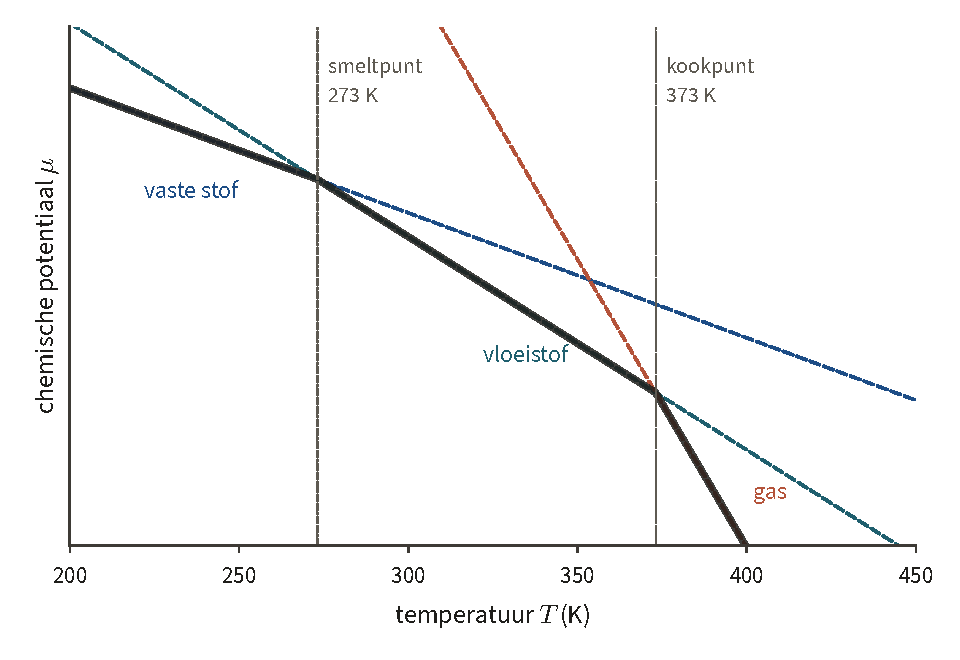
\includegraphics[width=0.7\linewidth]{Figuren/mu_temperatuur}
    \caption{Chemische potentiaal van vaste stof, vloeistof en gas van water bij \SI{1}{\bar} (schematisch op schaal, met $S_m$ = 41, 70 en \SI{189}{\joule\per\mole\per\kelvin}). De stabiele fase is telkens de laagste lijn (dik). De snijpunten zijn het smeltpunt en het kookpunt.}
    \label{fig:mu-T}
\end{figure}

Bij constante temperatuur stijgt $\mu$ met de druk, met helling $V_m$. Voor vloeistoffen en vaste stoffen is dat effect klein, voor gassen groot. Voor een ideaal gas ($V_m = RT/p$) geeft integratie vanaf de standaarddruk $p^\circ = \SI{1}{\bar}$:
\begin{equation}
\mu(T,p) = \mu^\circ(T) + RT \ln\frac{p}{p^\circ}.
\label{eq:mu-ideaalgas}
\end{equation}

\subsection{Fugaciteit: een veralgemening van de druk}
\label{sec:fugaciteit}
\label{sec:fugaciteitscoefficient}

Bij tientallen of honderden bar is een gas niet meer ideaal. Om de eenvoudige logaritmische vorm te behouden, vervangen we de druk door een effectieve druk, de \emph{fugaciteit} $f = \phi\,p$:
\begin{equation}
\mu = \mu^\circ + RT \ln\frac{f}{p^\circ} = \mu^\circ + RT \ln\frac{p}{p^\circ} + RT\ln\phi .
\end{equation}
De \emph{fugaciteitsco\"effici\"ent} $\phi$ meet de afwijking van ideaal gedrag ($\phi = 1$ voor een ideaal gas), net zoals de compressibiliteitsfactor $Z$ in hoofdstuk~\ref{ch:energie}. In de praktijk berekent men $\phi$ met een kubische toestandsvergelijking (Soave--Redlich--Kwong, Peng--Robinson).

\subsection{Activiteit: \'e\'en vorm voor elke fase}
\label{sec:activiteit}

In een ideaal gasmengsel draagt elke component bij met zijn partiële druk $p_i = y_ip$ (Dalton), zodat $\mu_i = \mu_i^\circ + RT\ln(p_i/p^\circ)$. Hetzelfde idee werkt voor elke fase.

\begin{definitie}{Chemische potentiaal via de activiteit}
Voor elke component $i$, in elke fase en bij elke samenstelling, geldt
\begin{equation}
\boxed{\mu_i = \mu_i^\circ + RT\ln a_i}
\label{eq:mu-activiteit}
\end{equation}
met $a_i$ de \emph{activiteit}: de dimensieloze ``effectieve concentratie'' die deze vergelijking exact maakt.
\end{definitie}

Voor een vloeistofmengsel schrijft men $a_i = \gamma_i x_i$, met $\gamma_i$ de \emph{activiteitsco\"effici\"ent}:
\begin{itemize}
\item $\gamma_i = 1$: ideaal gedrag, $a_i = x_i$ (voor een ideaal gas $a_i = p_i/p^\circ$);
\item $\gamma_i < 1$: de component voelt zich goed in het mengsel (sterkere aantrekking dan in zuivere toestand);
\item $\gamma_i > 1$: de component ``ontwijkt'' het mengsel;
\item een zuivere vloeistof of vaste stof in haar standaardtoestand heeft per afspraak $a_i = 1$.
\end{itemize}
Ethanol--water wijkt bijvoorbeeld zo sterk af van ideaal gedrag (waterstofbruggen) dat het een azeotroop vormt. Een kolomontwerp met $\gamma_i = 1$ zou daar volledig verkeerd uitkomen. Modellen voor $\gamma_i$ volgen in \S~\ref{sec:activiteitsmodellen}; in hoofdstuk~\ref{ch:reagerend} volstaan meestal $a_i \approx p_i/p^\circ$ en $a_i \approx 1$.

\subsection{Fase-evenwicht tussen twee fasen}
\label{sec:fase-evenwicht-voorwaarde}

Voor elke component geldt in evenwicht $\mu_i^{(\alpha)} = \mu_i^{(\beta)}$: tussen vast en vloeibaar, vloeistof en damp, twee vloeistoffen of twee kristalvormen. Bijna elk fase-evenwicht in de procestechnologie is een uitwerking van deze ene voorwaarde.


\subsection{De fasenregel van Gibbs}
\label{sec:fasenregel}

Hoeveel variabelen mag je vrij kiezen voor een systeem in evenwicht? Voor een zuivere stof die kookt, ligt de temperatuur vast zodra je de druk kiest: water kookt bij \SI{1}{atm} altijd bij \SI{100}{\celsius}. Voor een mengsel dat kookt, mag je ook nog de samenstelling kiezen. De \emph{fasenregel van Gibbs} telt dit precies:
\begin{equation}
\boxed{F = C - P + 2}
\label{eq:fasenregel}
\end{equation}
met $F$ het aantal \emph{vrijheidsgraden} (intensieve variabelen die je vrij kunt kiezen), $C$ het aantal componenten en $P$ het aantal fasen. De regel volgt uit een eenvoudige telling: elke fase heeft $T$, $p$ en $C-1$ onafhankelijke molfracties; elke component levert per extra fase \'e\'en evenwichtsvoorwaarde $\mu_i^{(\alpha)} = \mu_i^{(\beta)}$, en ook $T$ en $p$ zijn overal gelijk.
\begin{itemize}
\item Zuiver water, vloeistof + damp: $F = 1 - 2 + 2 = 1$. Kies $p$, dan ligt $T$ vast (de dampdruklijn).
\item Zuiver water op het tripelpunt: $F = 1 - 3 + 2 = 0$. Er is maar \'e\'en punt.
\item Benzeen--tolueen, vloeistof + damp: $F = 2 - 2 + 2 = 2$. Kies $p$ en $x$, dan liggen $T$ en $y$ vast. Dat is precies wat een VLE-diagram toont.
\end{itemize}

\section{Fase-evenwicht van zuivere stoffen: Clapeyron, Antoine en het fasediagram}

\subsection{De vergelijking van Clapeyron}
\label{sec:clapeyron}

Langs een evenwichtslijn blijven beide fasen in evenwicht, dus $\dd{\mu^{(\alpha)}} = \dd{\mu^{(\beta)}}$. Met $\dd{\mu} = V_m\,\dd{p} - S_m\,\dd{T}$ (vergelijking~\eqref{eq:dmu-fundamenteel}) voor elke fase en $\Delta S_{\text{trans}} = \Delta H_{\text{trans}}/T$ (hoofdstuk~\ref{ch:spontaniteit}) volgt de \emph{vergelijking van Clapeyron}:
\begin{equation}
\boxed{\;\frac{\dd{p}}{\dd{T}} = \frac{\Delta S_m}{\Delta V_m} = \frac{\Delta H_{\text{trans}}}{T\,\Delta V_m}\;}
\label{eq:clapeyron}
\end{equation}
Ze geldt voor elke faseovergang en geeft de helling van elke lijn in het fasediagram.

\begin{voorbeeld}{De smeltlijn van water}
IJs is minder dicht dan water, dus bij smelten is $\Delta V_m \approx \SI{-1.6e-6}{\metre\cubed\per\mole}$, met $\Delta H_{\text{fus}} = \SI{6.0}{\kilo\joule\per\mole}$:
\[
\frac{\dd{p}}{\dd{T}} = \frac{\SI{6000}{\joule\per\mole}}{(\SI{273.15}{\kelvin})(\SI{-1.6e-6}{\metre\cubed\per\mole})} \approx \SI{-140}{\bar\per\kelvin}.
\]
De helling is negatief: druk verlaagt het smeltpunt, maar je hebt \SI{140}{\bar} nodig voor \SI{1}{\kelvin}. Een schaatser haalt dat nauwelijks; de gladheid van ijs komt vooral van een dunne, vloeistofachtige oppervlaktelaag.
\end{voorbeeld}

\subsection{De vergelijking van Clausius--Clapeyron}
\label{sec:clausius-clapeyron}

Voor verdamping vereenvoudigt Clapeyron sterk: het dampvolume is veel groter dan het vloeistofvolume ($\Delta V_m \approx V_m^{(g)}$) en de damp is ongeveer ideaal ($V_m^{(g)} = RT/p$). Dan is $\dd{\ln p}/\dd{T} = \Delta H_{\text{vap}}/RT^2$, en met constante $\Delta H_{\text{vap}}$:
\begin{equation}
\boxed{\;\ln\frac{p_2}{p_1} = -\frac{\Delta H_{\text{vap}}}{R}\left(\frac{1}{T_2} - \frac{1}{T_1}\right)\;}
\label{eq:clausius-clapeyron-int}
\end{equation}
Een grafiek van $\ln p$ tegen $1/T$ is dus een rechte met helling $-\Delta H_{\text{vap}}/R$. Figuur~\ref{fig:dampdruk} toont hoe steil de dampdruk stijgt: elke \SI{20}{\kelvin} ongeveer een verdubbeling of meer.

\begin{figure}[htb]
    \centering
    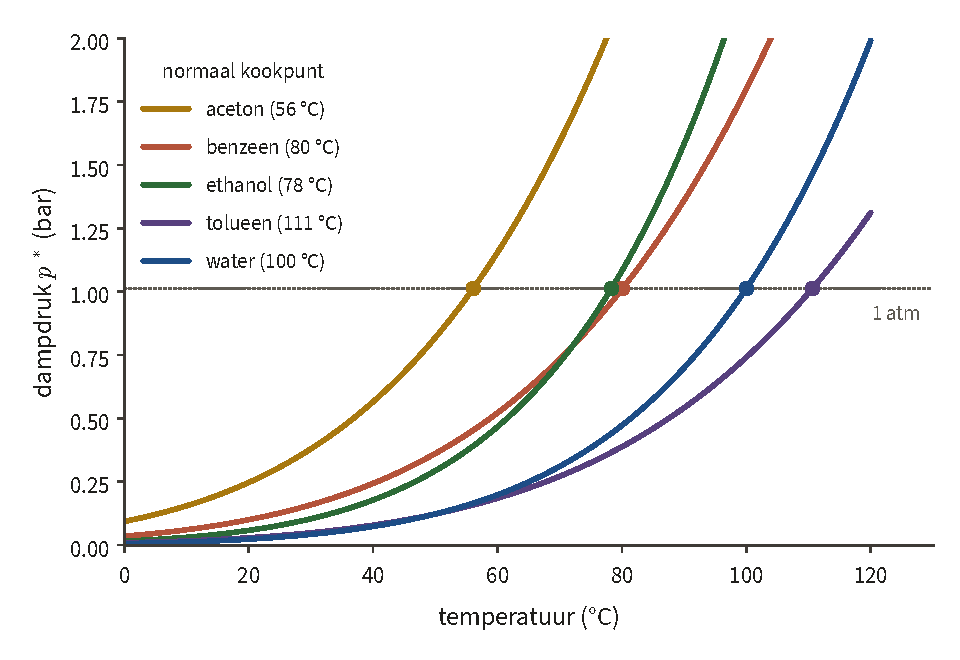
\includegraphics[width=0.7\linewidth]{Figuren/dampdruk}
    \caption{Dampdruk van vijf vloeistoffen. Waar een curve de lijn van \SI{1}{atm} snijdt, ligt het normale kookpunt. Benzeen en ethanol kruisen elkaar: bij kamertemperatuur is benzeen vluchtiger, boven ongeveer \SI{70}{\celsius} ethanol. Berekend met Antoine-constanten (bron: NIST WebBook; Dortmund Data Bank).}
    \label{fig:dampdruk}
\end{figure}

\begin{voorbeeld}{Dampdruk van water bij \SI{50}{\celsius}}
Uit het kookpunt ($p_1 = \SI{1.013}{\bar}$ bij \SI{373.15}{\kelvin}) en $\Delta H_{\text{vap}} = \SI{40.7}{\kilo\joule\per\mole}$:
\[
\ln\frac{p_2}{\SI{1.013}{\bar}} = -\frac{40700}{8.314}\left(\frac{1}{323.15} - \frac{1}{373.15}\right) = -3.42
\quad\Rightarrow\quad p_2 \approx \SI{36}{\milli\bar},
\]
dicht bij de gemeten \SI{35.6}{\milli\bar}.
\end{voorbeeld}

\subsection{De Antoine-vergelijking}
\label{sec:antoine}

Omdat $\Delta H_{\text{vap}}$ met de temperatuur verandert, gebruiken ingenieurs de empirische \emph{Antoine-vergelijking}:
\begin{equation}
\boxed{\;\log_{10} p^* = A - \frac{B}{T + C}\;}
\label{eq:antoine}
\end{equation}
De constanten $A$, $B$, $C$ staan in elke databank (NIST WebBook, Aspen Plus) en in de tabellenset.

\begin{voorbeeld}{Ethanol bij \SI{20}{\celsius}: controleer eerst de eenheden}
NIST geeft voor ethanol $A = 5.24677$, $B = 1598.673$, $C = -46.424$, met $p$ in bar en $T$ in kelvin. Andere bronnen gebruiken mmHg en \si{\celsius}, met totaal andere getallen. Controleer daarom eerst een bekend punt: bij $T = \SI{351.4}{\kelvin}$ geeft de formule \SI{1.013}{\bar}, het kookpunt van ethanol. Klopt. Dan bij \SI{293.15}{\kelvin}:
\[
\log_{10}p^* = 5.24677 - \frac{1598.673}{293.15 - 46.424} = -1.233
\quad\Rightarrow\quad p^* = \SI{58.5}{\milli\bar}
\]
(gemeten: \SI{59.5}{\milli\bar}).
\end{voorbeeld}

\subsection{Het fasediagram van een zuivere stof}
\label{sec:fasediagram}

De evenwichtslijnen samen vormen het \emph{fasediagram}: voor elke $(p, T)$ zie je welke fase stabiel is (figuur~\ref{fig:fasediagram}).

\begin{figure}[htb]
    \centering
    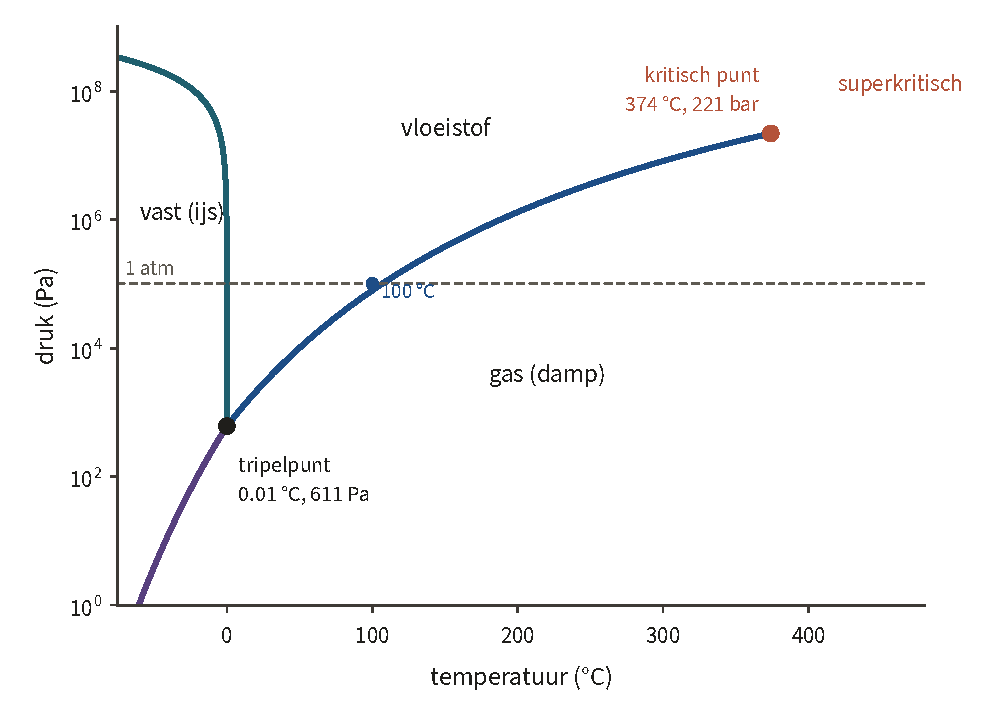
\includegraphics[width=0.7\linewidth]{Figuren/fasediagram}
    \caption{Fasediagram van water, met een logaritmische drukas. De dampdruklijn loopt van het tripelpunt tot het kritisch punt; de smeltlijn heeft een lichte \emph{negatieve} helling (hier overdreven getekend), zodat ijs bij hogere druk smelt. Bij \SI{1}{atm} kookt water bij \SI{100}{\celsius}.}
    \label{fig:fasediagram}
\end{figure}

\subsubsection{Het tripelpunt}
\label{sec:tripelpunt}

In het \emph{tripelpunt} bestaan drie fasen samen. Voor water: \SI{0.01}{\celsius} en \SI{611}{\pascal}. Onder die druk sublimeert ijs rechtstreeks: daarop berust vriesdrogen (koffie, vaccins).

\subsubsection{Het kritische punt}
\label{sec:kritisch-punt}

In het \emph{kritische punt} eindigt de dampdruklijn: vloeistof en damp worden ononderscheidbaar. Boven $T_c$ kan je een gas niet meer vloeibaar maken door samendrukken. Voor water: $T_c = \SI{374}{\celsius}$, $p_c = \SI{221}{\bar}$.

\subsubsection{Superkritische flu\"ida}
\label{sec:superkritisch}

Boven het kritische punt heeft een \emph{superkritisch flu\"idum} de dichtheid (en het oplosvermogen) van een vloeistof, maar diffundeert het als een gas. Superkritisch $\mathrm{CO_2}$ ($T_c = \SI{31}{\celsius}$, $p_c = \SI{74}{\bar}$) decaffe\"ineert koffie en extraheert hop, zonder resten van organisch solvent.

\section{Thermodynamica van mengsels en de wet van Raoult}

\subsection{Thermodynamica van mengsels}
\label{sec:thermodynamica-mengsels}

Ingenieurs werken bijna altijd met mengsels. In hoofdstuk~\ref{ch:spontaniteit} (\S~\ref{sec:waarschijnlijkheid-entropie}) zagen we dat mengen spontaan is door de toename van het aantal microtoestanden. Voor een \emph{ideaal} mengsel, waarin alle interacties even sterk zijn ($\Delta H_{\text{meng}} = 0$), geldt:
\begin{equation}
\Delta S_{\text{meng}} = -R \sum_i n_i \ln x_i > 0,
\qquad
\Delta G_{\text{meng}} = RT \sum_i n_i \ln x_i < 0.
\end{equation}

\begin{voorbeeld}{Minimale arbeid om lucht te scheiden}
Voor lucht ($x_{\mathrm{N_2}} = 0.79$, $x_{\mathrm{O_2}} = 0.21$) bij \SI{298}{\kelvin}:
\[
\Delta G_{\text{meng}} = RT(0.79\ln 0.79 + 0.21\ln 0.21) = \SI{-1.17}{\kilo\joule\per\mole}.
\]
Scheiden kost dus minstens \SI{1.17}{\kilo\joule} per mol lucht. Een cryogene luchtscheider haalt een rendement van 15 tot \SI{25}{\percent} van dat minimum.
\end{voorbeeld}

\subsubsection{Niet-ideale mengsels}
\label{sec:niet-ideale-mengsels}

Zijn de A--B-interacties zwakker dan de A--A- en B--B-interacties, dan is $\Delta H_{\text{meng}} > 0$ (hoofdstuk~\ref{ch:intermoleculair}, \S~\ref{sec:hildebrand}). In $\Delta G_{\text{meng}} = \Delta H_{\text{meng}} - T\Delta S_{\text{meng}}$ wordt het entropievoordeel dan deels of helemaal tenietgedaan. Figuur~\ref{fig:mengen-G} toont wat er gebeurt: bij een sterk endotherme menging krijgt de curve twee minima. Een mengsel tussen die minima valt spontaan uiteen in twee fasen (water en olie, \S~\ref{sec:lle}).

\begin{figure}[htb]
    \centering
    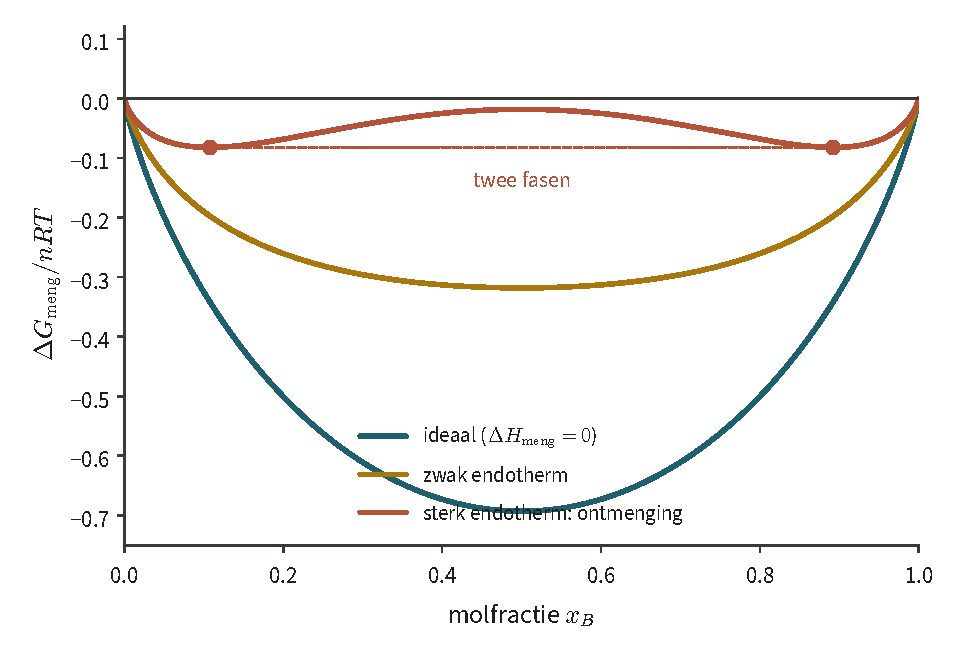
\includegraphics[width=0.7\linewidth]{Figuren/mengen_G}
    \caption{Gibbs-energie van mengen voor een binair mengsel met $\Delta H_{\text{meng}} = \chi RT\,x_A x_B$ (regelmatige oplossing). Voor $\chi > 2$ ontstaan twee minima: mengsels tussen de twee punten op de gemeenschappelijke raaklijn splitsen in twee vloeistoffasen.}
    \label{fig:mengen-G}
\end{figure}

\subsection{De chemische potentiaal in een mengsel}
\label{sec:mu-mengsel}

Afleiden van $G = \sum_i n_i \mu_i^* + RT \sum_i n_i \ln x_i$ naar $n_i$ geeft de chemische potentiaal in een ideaal mengsel:
\begin{equation}
\boxed{\;\mu_i = \mu_i^* + RT \ln x_i\;}
\label{eq:mu-mengsel-ideaal}
\end{equation}
Verdunnen verlaagt $\mu_i$: een component in een mengsel ``ontsnapt'' minder graag dan als zuivere stof.

\subsection{De wet van Raoult}
\label{sec:raoult}

Stel $\mu_i$ in de vloeistof (vergelijking~\eqref{eq:mu-mengsel-ideaal}) gelijk aan $\mu_i$ in de ideale damp, en je vindt de \emph{wet van Raoult}:
\begin{equation}
\boxed{\;p_i = x_i\,p_i^*\;}
\label{eq:raoult}
\end{equation}
De parti\"ele dampdruk is evenredig met de molfractie in de vloeistof; $p_i^*$ volgt uit Antoine. Voor een binair mengsel geeft Dalton de \emph{bubbelpuntsdruk} en de dampsamenstelling:
\begin{equation}
P = x_A p_A^* + x_B p_B^*, \qquad y_i = \frac{x_i p_i^*}{P}.
\end{equation}

\begin{voorbeeld}{Benzeen--tolueen bij \SI{90}{\celsius}}
Met $x_A = 0.40$ benzeen, $p_A^* = \SI{1.35}{\bar}$ en $p_B^* = \SI{0.54}{\bar}$:
\[
P = 0.40 \cdot 1.35 + 0.60 \cdot 0.54 = \SI{0.864}{\bar}, \qquad y_A = \frac{0.40 \cdot 1.35}{0.864} = 0.625.
\]
De damp bevat \SI{62.5}{\percent} benzeen, de vloeistof maar \SI{40}{\percent}. Dat verschil is de basis van destillatie.
\end{voorbeeld}

\subsection{Relatieve vluchtigheid}
\label{sec:relatieve-vluchtigheid}

Hoe makkelijk twee componenten door destillatie te scheiden zijn, vat de \emph{relatieve vluchtigheid} samen:
\begin{equation}
\boxed{\;\alpha_{AB} = \frac{y_A/x_A}{y_B/x_B} = \frac{p_A^*}{p_B^*}\;}
\end{equation}
(de tweede gelijkheid voor ideale mengsels). Bij $\alpha \approx 1$ is destillatie praktisch onmogelijk, bij $\alpha \approx 2$ eenvoudig, en bij $\alpha \geq 5$ zeer eenvoudig. Voor benzeen--tolueen bij \SI{90}{\celsius} is $\alpha = 1.35/0.54 = 2.5$: een klassiek, goed scheidbaar mengsel.

\section{Het damp-vloeistofdiagram: hefboomwet en azeotropen}

\subsection{Zelf een VLE-diagram opstellen}
\label{sec:vle-diagram}

Een damp-vloeistofdiagram (VLE-diagram) toont voor een binair mengsel welke vloeistof met welke damp in evenwicht is. Voor een ideaal mengsel kun je het volledig zelf opstellen met twee ingredi\"enten: de wet van Raoult en de dampdrukken van de zuivere componenten (Antoine, \S~\ref{sec:antoine}). Er zijn drie gangbare voorstellingen.

\subsubsection{Het $P$--$x$--$y$-diagram (constante temperatuur)}

Kies de temperatuur, bereken $p_A^*$ en $p_B^*$, en doorloop $x_A$ van 0 tot 1:
\begin{enumerate}
\item bubbelpuntdruk: $P = x_A p_A^* + (1 - x_A) p_B^*$;
\item dampsamenstelling: $y_A = x_A p_A^*/P$;
\item zet $P$ uit tegen $x_A$ (de \emph{bubbelpuntlijn}, een rechte) en tegen $y_A$ (de \emph{dauwpuntlijn}, gekromd).
\end{enumerate}
Boven de bubbelpuntlijn is het mengsel volledig vloeibaar, onder de dauwpuntlijn volledig damp. Daartussen liggen vloeistof en damp naast elkaar (figuur~\ref{fig:vle-diagram}). Een horizontale lijn in dat gebied verbindt een vloeistof met de damp waarmee ze in evenwicht is: een \emph{bindlijn}.

\begin{figure}[htb]
    \centering
    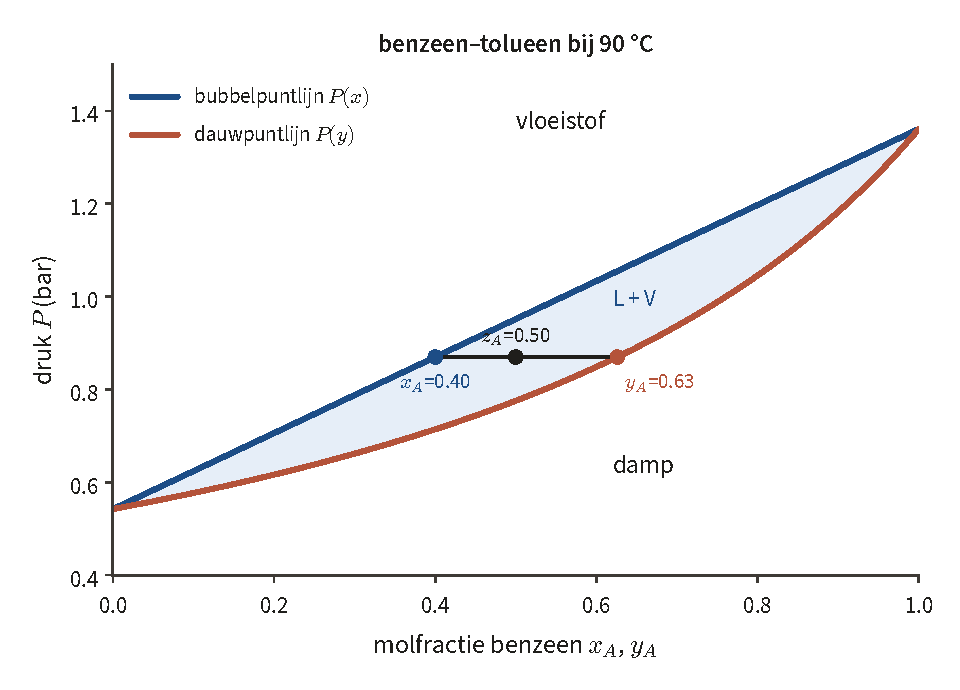
\includegraphics[width=0.75\linewidth]{Figuren/pxy_benzeen_tolueen}
    \caption{$P$--$x$--$y$-diagram van benzeen (A) en tolueen (B) bij \SI{90}{\celsius}, berekend met de wet van Raoult en de Antoinevergelijking. De bindlijn bij $P \approx \SI{0.87}{\bar}$ verbindt vloeistof met $x_A = 0.40$ en damp met $y_A = 0.63$; het punt $z_A = 0.50$ hoort bij het voorbeeld van de hefboomwet (\S~\ref{sec:hefboomwet}).}
    \label{fig:vle-diagram}
\end{figure}

\subsubsection{Het $T$--$x$--$y$-diagram (constante druk)}

In een destillatiekolom ligt de druk vast en varieert de temperatuur. Het $T$--$x$--$y$-diagram is daarom het meest gebruikte. Het opstellen vraagt \'e\'en extra stap, omdat $p^*$ afhangt van de onbekende temperatuur:
\begin{enumerate}
\item kies $x_A$;
\item zoek de temperatuur waarbij $x_A p_A^*(T) + (1 - x_A) p_B^*(T) = P$. Dat is een vergelijking in \'e\'en onbekende, op te lossen met \emph{Doelzoeken} in Excel of door een paar temperaturen te proberen;
\item bereken $y_A = x_A p_A^*(T)/P$;
\item herhaal voor andere $x_A$ en zet $T$ uit tegen $x_A$ en $y_A$.
\end{enumerate}
De bubbelpuntlijn ligt nu \emph{onder}: een vloeistof begint te koken wanneer je ze opwarmt tot op die lijn. De dauwpuntlijn ligt erboven (figuur~\ref{fig:txy}).

\begin{voorbeeld}{Kookpunt van een benzeen--tolueenmengsel bij 1 atm}
Gevraagd: de kooktemperatuur en de eerste damp van een vloeistof met $x_A = 0.40$ bij $P = \SI{1.013}{\bar}$. Antoine (\si{mmHg}, \si{\celsius}): benzeen $A = 6.90565$, $B = 1211.033$, $C = 220.790$; tolueen $A = 6.95464$, $B = 1344.800$, $C = 219.482$.

Probeer \SI{95}{\celsius}: $p_A^* = \SI{1.569}{\bar}$, $p_B^* = \SI{0.636}{\bar}$, en $0.40(1.569) + 0.60(0.636) = \SI{1.009}{\bar}$: net te laag. Bij \SI{95.1}{\celsius} klopt de som. Daar is $y_A = 0.40 \times 1.575/1.013 = 0.62$.

De eerste damp bevat dus 62\,\% benzeen, tegenover 40\,\% in de vloeistof. Condenseer je die damp en laat je hem opnieuw koken, dan wordt hij nog rijker. Dat is het principe van een destillatiekolom: elke schotel is een nieuwe stap tussen de bubbelpunt- en de dauwpuntlijn.
\end{voorbeeld}

\subsubsection{Het $x$--$y$-diagram}

Zet je voor elk punt $y_A$ uit tegen $x_A$, dan krijg je de \emph{evenwichtslijn} van het $x$--$y$-diagram (figuur~\ref{fig:txy}, rechts). Hoe verder die lijn boven de diagonaal $y = x$ ligt, hoe gemakkelijker de scheiding. Voor een ideaal mengsel met constante relatieve vluchtigheid $\alpha$ geldt
\begin{equation}
y_A = \frac{\alpha\,x_A}{1 + (\alpha - 1)\,x_A}.
\label{eq:xy-alpha}
\end{equation}
Dit diagram is het vertrekpunt van de grafische methode van McCabe--Thiele, waarmee je in de cursus Scheidingstechnologie het aantal schotels van een destillatiekolom bepaalt.

\begin{figure}[htb]
    \centering
    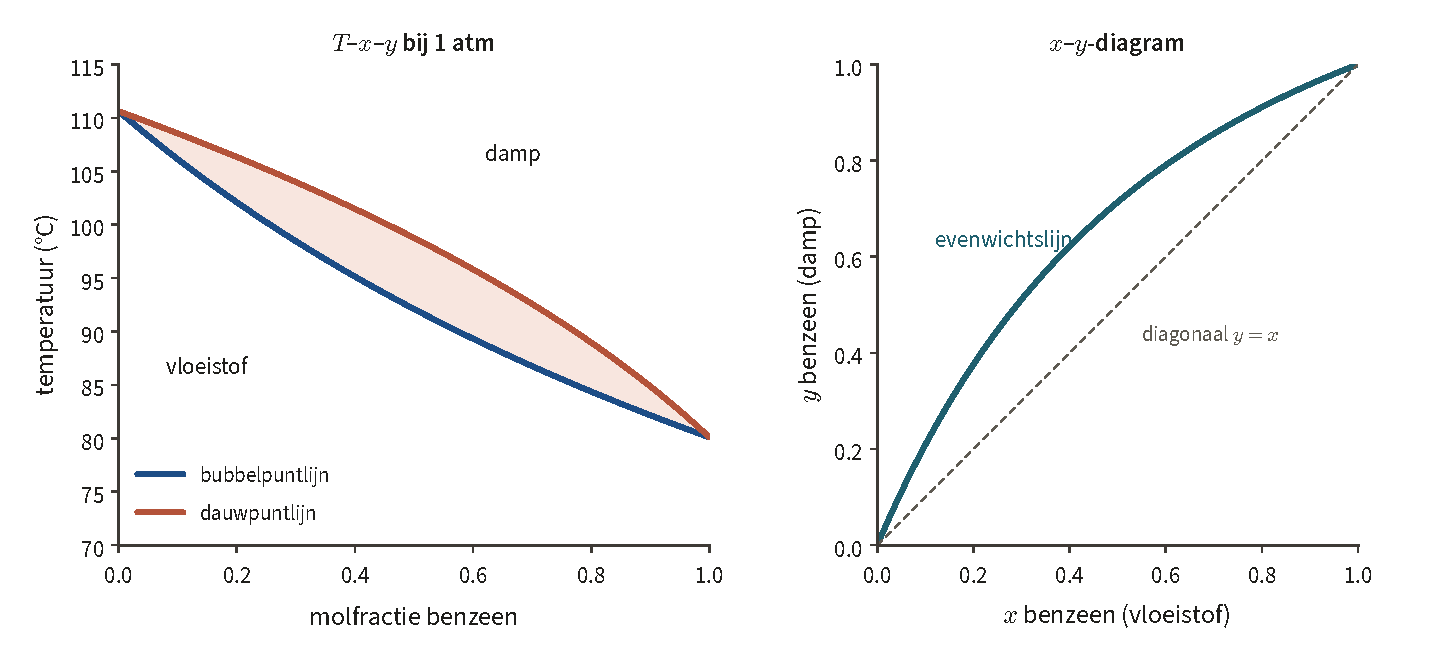
\includegraphics[width=\linewidth]{Figuren/txy_benzeen_tolueen}
    \caption{Links: $T$--$x$--$y$-diagram van benzeen--tolueen bij \SI{1}{atm}. Rechts: het bijbehorende $x$--$y$-diagram. Beide berekend met Raoult en Antoine; zuiver benzeen kookt bij \SI{80.1}{\celsius}, zuiver tolueen bij \SI{110.6}{\celsius}.}
    \label{fig:txy}
\end{figure}

\subsection{De hefboomwet (lever rule)}
\label{sec:hefboomwet}

Wanneer een mengsel zich in het tweefasengebied bevindt, geldt een massabalans die de verhouding van vloeistof en damp vastlegt. Beschouw een totaal aantal mol $n_{\text{tot}}$ met globale molfractie $z_A$, dat splitst in een vloeistoffase ($n_L$, molfractie $x_A$) en een dampfase ($n_V$, molfractie $y_A$). De massabalans voor component $A$ luidt:
\[
n_{\text{tot}} z_A = n_L x_A + n_V y_A.
\]
Met $n_{\text{tot}} = n_L + n_V$ volgt na herschikking de \emph{hefboomwet}:
\begin{equation}
\boxed{\;\frac{n_L}{n_V} = \frac{y_A - z_A}{z_A - x_A}\;}
\label{eq:hefboomwet}
\end{equation}
De verhouding van vloeistof- en damphasen wordt dus bepaald door de afstand van het globale punt tot de bubbelpunt- en dauwpuntcurve, analoog aan een hefboom rond een steunpunt.

\begin{voorbeeld}{Toepassing van de hefboomwet}
Voor het benzeen--tolueenmengsel bij \SI{90}{\celsius} en $P = \SI{0.864}{\bar}$ geldt $x_A = 0.40$ en $y_A = 0.625$ (uit het eerdere voorbeeld). Een globale samenstelling $z_A = 0.50$ geeft:
\[
\frac{n_L}{n_V} = \frac{0.625 - 0.50}{0.50 - 0.40} = \frac{0.125}{0.10} = 1.25.
\]
Van elke mol mengsel bevindt zich dus $n_L = 0.56$ mol in de vloeistoffase en $n_V = 0.44$ mol in de dampfase. Deze eenvoudige berekening vormt het vertrekpunt van het ontwerp van een destillatiekolom.
\end{voorbeeld}

\subsection{Azeotropen}
\label{sec:azeotropen}

Re\"ele mengsels wijken af van Raoult. Is de afwijking groot genoeg, dan krijgt de $P$--$x$-curve een maximum of minimum. Daar zijn vloeistof en damp even samengesteld: een \emph{azeotroop} (figuur~\ref{fig:azeotroop}). Destillatie raakt daar niet voorbij.

\begin{figure}[htb]
    \centering
    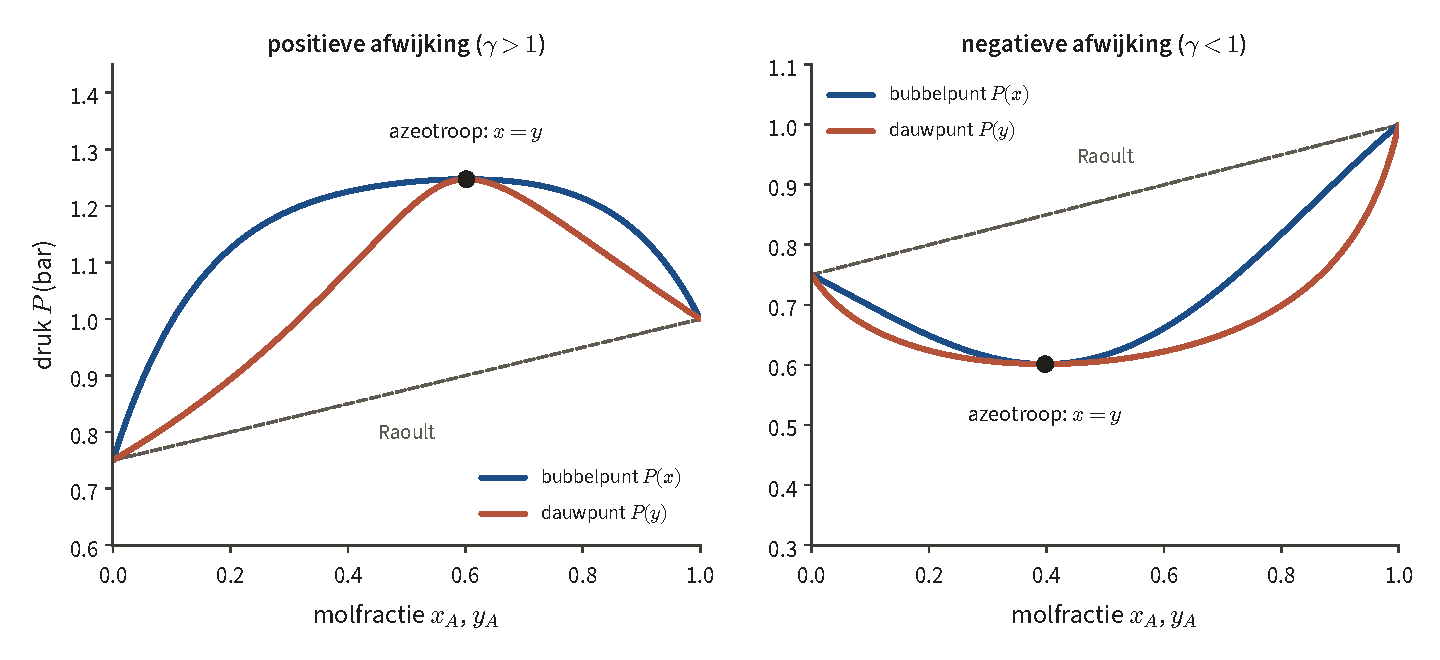
\includegraphics[width=\linewidth]{Figuren/azeotroop}
    \caption{$P$--$x$--$y$-diagrammen bij constante temperatuur voor een mengsel met positieve (links) en negatieve (rechts) afwijking van Raoult (Margules, $A = \pm 1.4$). In het extremum raken bubbelpunt- en dauwpuntlijn elkaar: de azeotroop. De stippellijn is de wet van Raoult.}
    \label{fig:azeotroop}
\end{figure}

\begin{itemize}
\item \textbf{Positieve afwijking} (A--B-interacties zwakker): dampdruk boven Raoult, dus een \emph{minimaal kokende} azeotroop. Ethanol--water kookt bij \SI{78.2}{\celsius} en $x_{\text{eth}} = 0.894$ (\SI{95.6}{\percent} in massa), net onder zuiver ethanol (\SI{78.4}{\celsius}). Daarom haal je met gewone destillatie geen zuiverdere ethanol.
\item \textbf{Negatieve afwijking} (A--B-interacties sterker): dampdruk onder Raoult, dus een \emph{maximaal kokende} azeotroop. Aceton--chloroform kookt bij \SI{64.5}{\celsius}, boven beide zuivere stoffen, door een waterstofbrug tussen \ce{C=O} en \ce{Cl3C-H} (hoofdstuk~\ref{ch:intermoleculair}, \S~\ref{sec:waterstofbruggen}). Zoutzuur--water kookt constant bij \SI{110}{\celsius} en \SI{20}{\percent} HCl.
\end{itemize}

\section{Re\"ele mengsels: activiteit en activiteitsco\"effici\"entmodellen}

\subsection{Re\"ele mengsels en activiteit}
\label{sec:activiteit-mengsel}

Voor re\"ele mengsels vervangen we de molfractie door de activiteit (\S~\ref{sec:activiteit}), met de \emph{activiteitsco\"effici\"ent} $\gamma_i$ als correctiefactor:
\begin{equation}
\mu_i = \mu_i^* + RT \ln a_i, \qquad
\boxed{\;a_i = \gamma_i\,x_i\;}
\label{eq:activiteit-mengsel}
\end{equation}
Raoult wordt dan $p_i = \gamma_i x_i p_i^*$ (gemodificeerde Raoult). Bij $\gamma_i > 1$ ontsnapt de component makkelijker dan ideaal (positieve afwijking), bij $\gamma_i < 1$ wordt hij beter vastgehouden (negatieve afwijking). Voor de zuivere stof ($x_i \to 1$) gaat $\gamma_i$ altijd naar 1.

\subsubsection{De wet van Henry}
\label{sec:henry}

Een sterk verdunde component is volledig omringd door oplosmiddel. Zijn ``ontsnappingsneiging'' hangt dan af van de interactie met dat oplosmiddel, niet met zijn eigen soort, en $\gamma_i$ wordt constant ($\gamma_i^\infty$). Dat geeft de \emph{wet van Henry}:
\begin{equation}
\boxed{\;p_i = x_i\,H_i\;}
\label{eq:henry}
\end{equation}
met $H_i = \gamma_i^\infty p_i^*$ een eigenschap van het paar opgeloste stof--oplosmiddel. In dezelfde oplossing volgt het oplosmiddel dus Raoult en de opgeloste stof Henry (figuur~\ref{fig:raoult-henry}). Henry beschrijft vooral de oplosbaarheid van gassen ($\mathrm{O_2}$, $\mathrm{CO_2}$, $\mathrm{N_2}$) in water.

\begin{figure}[htb]
    \centering
    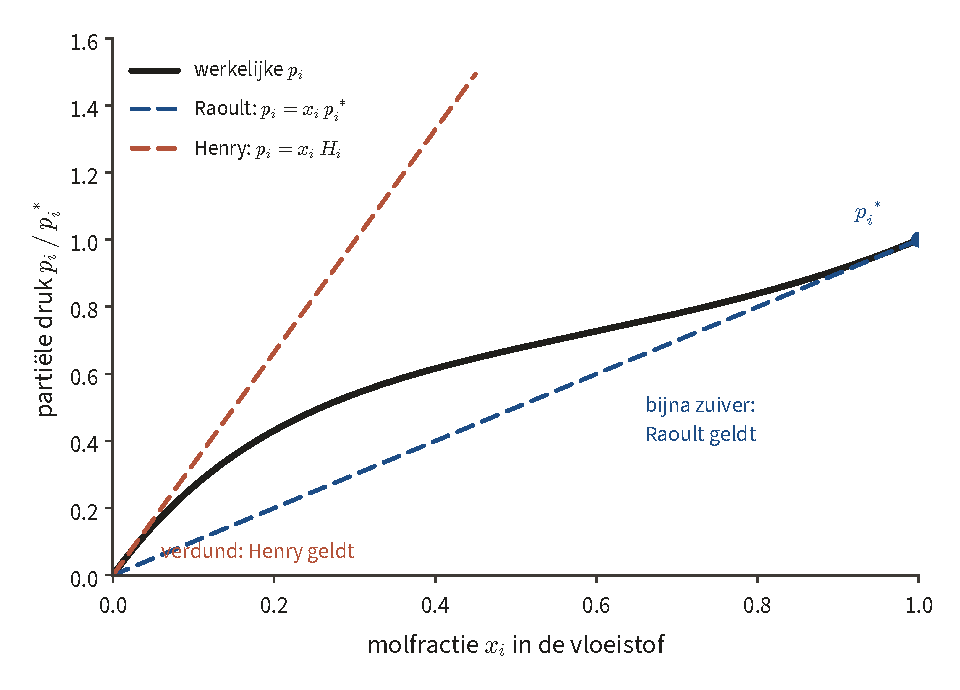
\includegraphics[width=0.7\linewidth]{Figuren/raoult_henry}
    \caption{Parti\"ele dampdruk van een component met positieve afwijking van Raoult. Bij hoge molfractie (bijna zuiver) volgt de curve de wet van Raoult; in sterke verdunning volgt ze de wet van Henry, met een andere helling $H_i$. Daartussen is een activiteitsco\"effici\"entmodel nodig.}
    \label{fig:raoult-henry}
\end{figure}

\begin{voorbeeld}{Waarom een fles spuitwater bruist}
Voor $\mathrm{CO_2}$ in water bij \SI{25}{\celsius} is $H \approx \SI{1640}{\bar}$. Onder \SI{3}{\bar} $\mathrm{CO_2}$ in de fles is $x_{\mathrm{CO_2}} = 3/1640 = 1.8\times10^{-3}$. Na openen is $p_{\mathrm{CO_2}} \approx \SI{4e-4}{\bar}$ en zakt het evenwicht naar $2.4\times10^{-7}$: \num{7500} keer minder. Het overtollige gas komt vrij als bellen.
\end{voorbeeld}

\paragraph{Let op de eenheden.}
Tabellen geven vaak de oplosbaarheid $k_\mathrm{H} = c_i/p_i$ in \si{\mole\per\litre\per\bar}. Voor verdunde waterige oplossingen (\SI{55.5}{\mole} water per liter) is $H_i\,(\si{\bar}) \approx 55.5/k_\mathrm{H}$. Een verwisseling geeft al snel een factor $10^4$ fout.

\paragraph{Temperatuur.}
Gassen lossen bijna altijd \emph{slechter} op bij hogere temperatuur: oplossen is exotherm (Le Chatelier). Zoals bij Clausius--Clapeyron is $\ln k_\mathrm{H}$ ongeveer lineair in $1/T$.

\begin{toepassing}{Zuurstof in water: van vissenkom tot stoomketel}
Voor zuurstof in water bij \SI{25}{\celsius} is $k_\mathrm{H} = \SI{1.3e-3}{\mole\per\litre\per\bar}$. Met \SI{0.21}{\bar} zuurstof in lucht geeft dat $c_{\ce{O2}} = \SI{2.7e-4}{\mole\per\litre} \approx \SI{8.7}{\milli\gram\per\litre}$. Bij \SI{5}{\celsius} is dat ongeveer \SI{13}{\milli\gram\per\litre}, bij \SI{35}{\celsius} nog \SI{7.3}{\milli\gram\per\litre}. Vissen hebben minstens \SIrange{4}{5}{\milli\gram\per\litre} nodig: in een warme zomernacht wordt het kritiek, en waterzuiveringen blazen daarom lucht in.

Een stoomketel wil net \emph{geen} zuurstof, omdat die het staal corrodeert (hoofdstuk~\ref{ch:elektrochemie}). In een \emph{ontgasser} wordt het voedingswater met stoom tot het kookpunt verwarmd; de stoom voert de vrijgekomen zuurstof af tot onder \SI{10}{\micro\gram\per\litre}.
\end{toepassing}

\subsection{Modellen voor activiteitsco\"effici\"enten}
\label{sec:activiteitsmodellen}

Om $\gamma_i$ te berekenen gebruikt men modellen met enkele parameters, gefit op metingen. Het eenvoudigste is \emph{Margules met \'e\'en parameter}:
\begin{equation}
\ln \gamma_A = A\, x_B^2, \qquad \ln \gamma_B = A\, x_A^2.
\end{equation}
$A > 0$ geeft positieve en $A < 0$ negatieve afwijking; bij oneindige verdunning is $\gamma^\infty = e^A$ (figuur~\ref{fig:margules}). Voor aceton--chloroform bij \SI{35}{\celsius} is $A = -0.84$, zodat bij $x = 0.5$: $\gamma = e^{-0.21} = 0.81$.

\begin{figure}[htb]
    \centering
    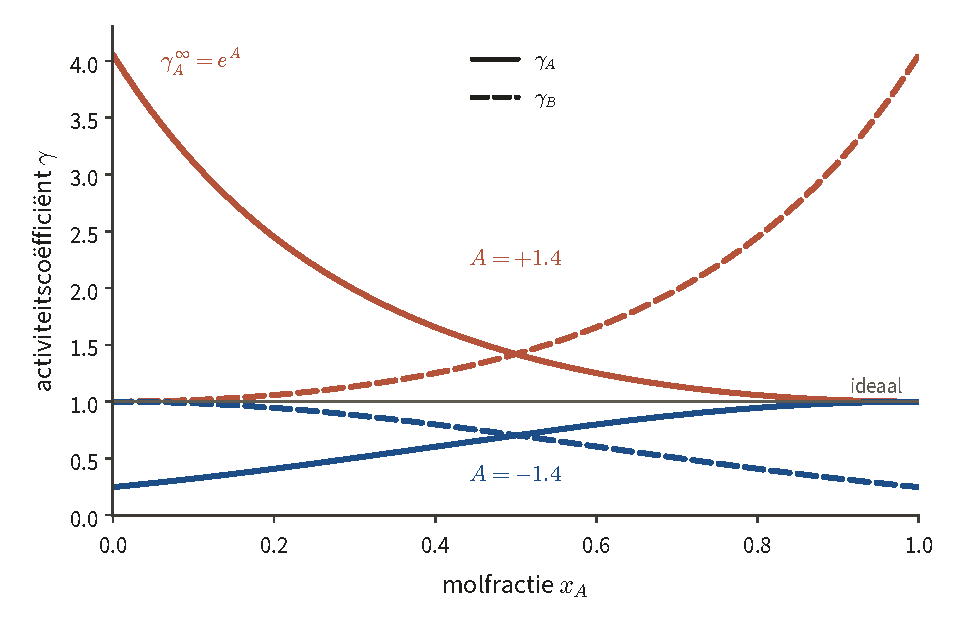
\includegraphics[width=0.7\linewidth]{Figuren/margules}
    \caption{Activiteitsco\"effici\"enten volgens Margules (\'e\'en parameter). Elke component nadert $\gamma = 1$ als hij bijna zuiver is, en wijkt het sterkst af bij oneindige verdunning. Deze $\gamma$'s leveren de azeotropen van figuur~\ref{fig:azeotroop}.}
    \label{fig:margules}
\end{figure}

Re\"ele mengsels zijn vaak asymmetrisch. Daarvoor bestaan modellen met twee of drie parameters (tabel~\ref{tab:gamma-modellen}). Je hoeft hun formules niet te kennen: processimulators zoals Aspen Plus bevatten ze, samen met parameters uit databanken. Belangrijk is wel te weten wat elk model kan.

\begin{table}[htb]
\centering
\small
\begin{tabular}{lcl}
\toprule
Model & Parameters & Geschikt voor \\
\midrule
Margules (1 of 2) & 1--2 & snelle schatting, onderwijs \\
Van Laar & 2 & eenvoudige niet-ideale mengsels \\
Wilson & 2 & volledig mengbare mengsels; \emph{geen} LLE \\
NRTL & 3 & algemeen: VLE \'en LLE \\
UNIQUAC & 2 & zoals NRTL, houdt rekening met molecuulgrootte \\
\bottomrule
\end{tabular}
\caption{Activiteitsco\"effici\"entmodellen voor vloeistofmengsels. In de procesindustrie zijn Wilson en NRTL het meest gebruikt.}
\label{tab:gamma-modellen}
\end{table}

\section{Vloeistof-vloeistof- en vast-vloeistofevenwicht}

\subsection{Vloeistof-vloeistofevenwicht (LLE)}
\label{sec:lle}

Is $\Delta H_{\text{meng}}$ sterk positief (zeer verschillende Hildebrand-parameters, hoofdstuk~\ref{ch:intermoleculair}), dan krijgt $\Delta G_{\text{meng}}$ twee minima en splitst het mengsel in twee vloeistoffasen (figuur~\ref{fig:mengen-G}): water--olie, water--fenol, polymeer--oplosmiddel. Dat \emph{vloeistof-vloeistofevenwicht} is de basis van extractie, nuttig voor componenten die moeilijk te destilleren zijn.

\subsubsection{De Nernst-verdelingswet}
\label{sec:nernst}

Een component die verdeeld raakt over twee onmengbare fasen heeft in beide dezelfde $\mu$. In verdunde oplossing geeft dat een constante verhouding, de \emph{verdelingswet van Nernst}:
\begin{equation}
\boxed{\;K_D = \frac{c_i^{(\alpha)}}{c_i^{(\beta)}}\;}
\label{eq:nernst-verdeling}
\end{equation}

\begin{voorbeeld}{Extractie van jodium}
Jodium verdeelt zich tussen $\mathrm{CCl_4}$ en water met $K_D \approx 86$. Extraheer je \SI{1}{\litre} waterige oplossing (\SI{0.1}{\mole\per\litre}) met \SI{0.5}{\litre} $\mathrm{CCl_4}$, dan blijft in het water
\[
c_{\text{water}} = 0.1 \cdot \frac{V_w}{V_w + K_D V_o} = 0.1 \cdot \frac{1}{1 + 86 \cdot 0.5} = \SI{0.0023}{\mole\per\litre}.
\]
E\'en stap verwijdert dus \SI{97.7}{\percent} van het jodium.
\end{voorbeeld}

\subsubsection{Ternaire diagrammen}
\label{sec:ternair}

Bij vloeistof-vloeistofextractie zijn er minstens drie componenten: de \emph{drager} (bv.\ water), de \emph{opgeloste stof} die je wilt winnen (bv.\ aceton) en het \emph{extractiemiddel} (bv.\ methylisobutylketon, MIBK). Hun evenwicht stel je voor in een \emph{ternair diagram}: een gelijkzijdige driehoek (figuur~\ref{fig:ternair}).
\begin{itemize}
\item Elke hoek is een zuivere component; elke zijde een binair mengsel.
\item Een punt binnen de driehoek is een mengsel van alle drie. De massafractie van een component lees je af als de afstand tot de zijde tegenover zijn hoek: op die zijde is ze 0, in de hoek 1. De drie fracties tellen altijd op tot 1.
\item De \emph{binodale curve} begrenst het gebied waarin het mengsel in twee vloeistoffasen uiteenvalt. Binnen dat gebied verbinden \emph{bindlijnen} de twee fasen die met elkaar in evenwicht zijn: het \emph{raffinaat} (waterrijk, links) en het \emph{extract} (MIBK-rijk, rechts).
\item Waar de bindlijnen krimpen tot een punt, worden beide fasen identiek: het \emph{plooipunt}.
\end{itemize}

Het belangrijkste rekeninstrument is opnieuw de hefboomwet. Meng je twee stromen F en S, dan ligt het mengpunt M op de rechte FS, en de verhouding van de hoeveelheden is omgekeerd evenredig met de afstanden: $m_\mathrm{F}/m_\mathrm{S} = \overline{\mathrm{MS}}/\overline{\mathrm{MF}}$. Valt M in het tweefasengebied, dan splitst het mengsel langs de bindlijn door M in raffinaat R en extract E.

\begin{figure}[htb]
    \centering
    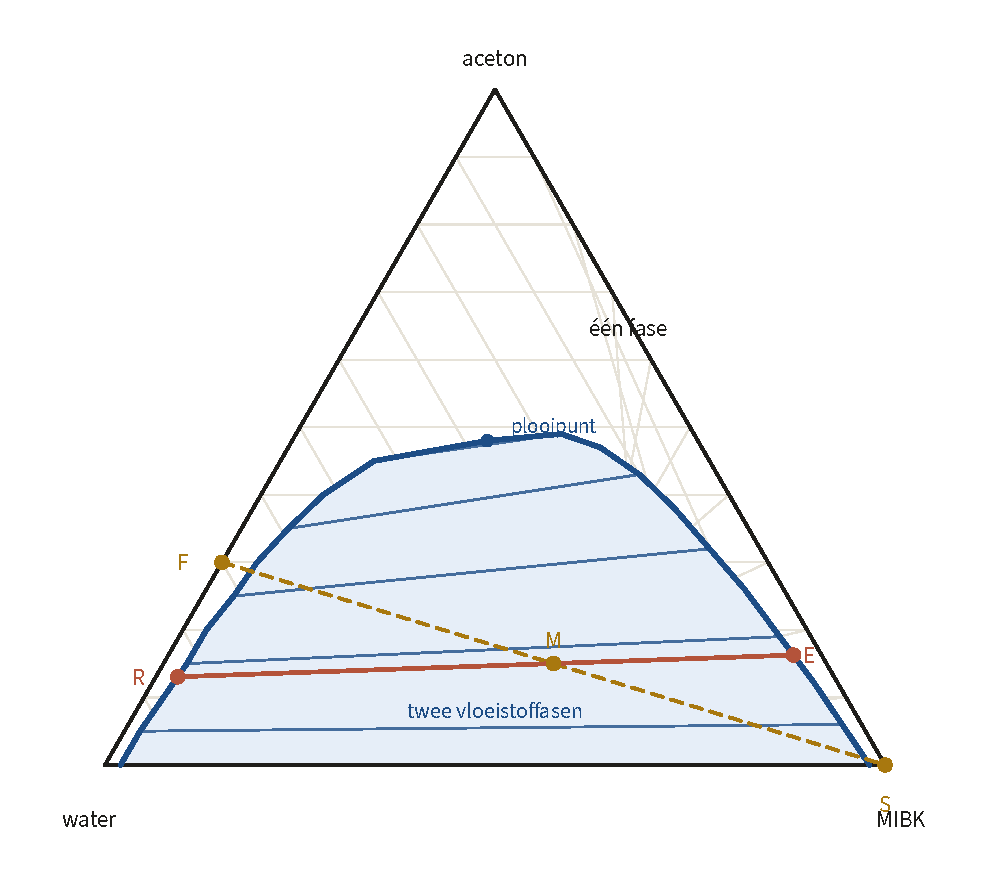
\includegraphics[width=0.72\linewidth]{Figuren/ternair}
    \caption{Ternair diagram water--aceton--MIBK bij \SI{25}{\celsius} (massafracties, benaderende waarden). Binnen de binodale curve vormen zich twee vloeistoffasen, verbonden door bindlijnen. Het voorbeeld: voeding F (30\,\% aceton in water) wordt gemengd met evenveel zuiver MIBK (S) tot M, dat splitst in raffinaat R en extract E.}
    \label{fig:ternair}
\end{figure}

\begin{voorbeeld}{Aceton uit water extraheren met MIBK}
\SI{100}{\kilo\gram} water met \SI{30}{\percent} aceton wordt gemengd met \SI{100}{\kilo\gram} zuiver MIBK.

\textbf{Mengpunt.} Het mengsel van \SI{200}{\kilo\gram} bevat 30 kg aceton, 70 kg water en 100 kg MIBK: M = (15\,\% aceton, 35\,\% water, 50\,\% MIBK). Dat ligt in het midden van de rechte FS, en binnen de binodale curve.

\textbf{Bindlijn.} De bindlijn door M (figuur~\ref{fig:ternair}) geeft het raffinaat R = (13\,\% aceton, 84\,\% water, 3\,\% MIBK) en het extract E = (16\,\% aceton, 4\,\% water, 80\,\% MIBK).

\textbf{Hefboomwet.} Met een acetonbalans: $200 \times 0.15 = 0.130\,m_\mathrm{R} + 0.163\,m_\mathrm{E}$ en $m_\mathrm{R} + m_\mathrm{E} = 200$, dus $m_\mathrm{E} = \SI{121}{\kilo\gram}$ en $m_\mathrm{R} = \SI{79}{\kilo\gram}$.

Het extract bevat $121 \times 0.163 = \SI{19.7}{\kilo\gram}$ aceton: twee derde van de aceton is in \'e\'en stap overgegaan naar het MIBK. Het raffinaat bevat nog \SI{10}{\kilo\gram} aceton. Met een tweede extractiestap op het raffinaat, of een tegenstroomkolom, haal je bijna alles. Hoeveel stappen nodig zijn, leer je in de cursus Scheidingstechnologie.
\end{voorbeeld}

\subsection{Vast-vloeistofevenwicht (SLE)}
\label{sec:sle}

Het evenwicht tussen een vaste stof en een vloeistof speelt een centrale rol bij kristallisatie, legeringen en zuiveringsprocessen. Net als bij VLE wordt het SLE bepaald door de gelijkheid van de chemische potentialen, maar de rol van beide fasen is gewijzigd.

\subsubsection{Eutectische diagrammen}
\label{sec:eutecticum}

Voor een binair systeem $A$--$B$ met beperkte vaste-mengbaarheid vertoont het fasediagram een \emph{eutecticum}. Het \emph{eutectisch punt} is de combinatie van samenstelling en temperatuur waarbij vloeistof, vaste stof $A$ en vaste stof $B$ (of twee vaste oplossingen) gelijktijdig co\"existeren. Bij afkoelen van een vloeistof met eutectische samenstelling stollen beide componenten simultaan bij een vaste temperatuur, analoog aan een zuivere stof.

Voor mengsels met een andere samenstelling begint de stolling bij een hogere temperatuur, waarbij eerst de ene component als vaste fase uitkristalliseert. De resterende vloeistof verandert in samenstelling langs de \emph{liquidus}-curve naarmate de temperatuur daalt, tot het eutectisch punt wordt bereikt.

\begin{figure}[htb]
    \centering
    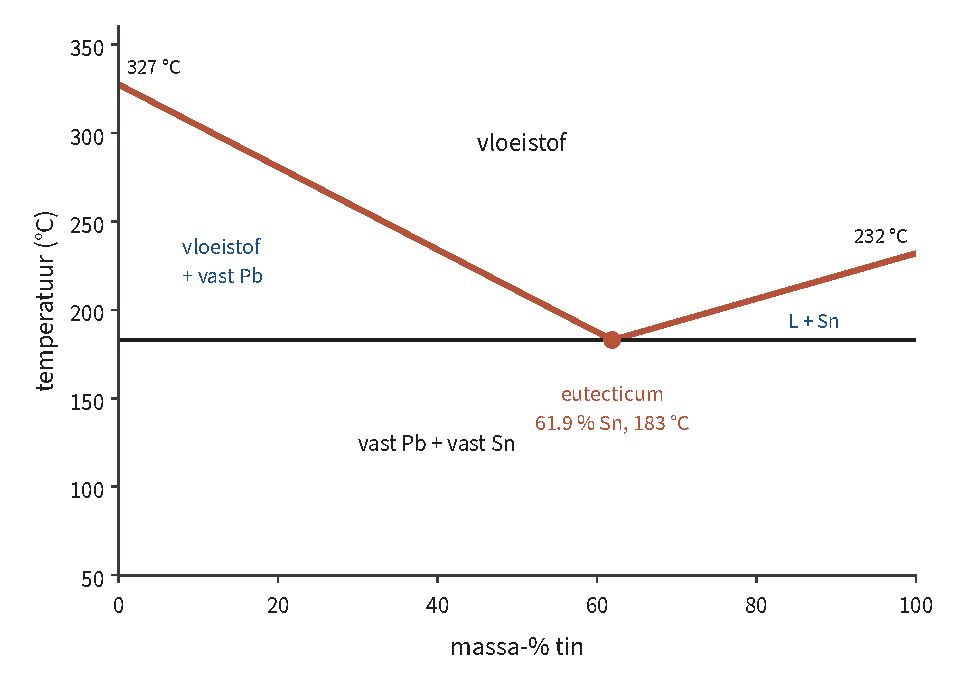
\includegraphics[width=0.7\linewidth]{Figuren/eutecticum}
    \caption{Vereenvoudigd eutectisch diagram van lood--tin (de beperkte vaste oplosbaarheid aan beide kanten is weggelaten). De liquiduslijnen dalen vanuit de smeltpunten van lood (\SI{327}{\celsius}) en tin (\SI{232}{\celsius}) tot het eutecticum bij \num{61.9}~massaprocent tin en \SI{183}{\celsius}.}
    \label{fig:eutecticum}
\end{figure}

Typische voorbeelden:
\begin{itemize}
\item Lood--tin (Pb--Sn) met eutecticum bij \num{61.9}~massaprocent tin ($x_{\text{Sn}} = 0.74$) en $T = \SI{183}{\celsius}$: de basis van klassiek soldeertin. Omdat lood giftig is, gebruikt men vandaag tin--zilver--koperlegeringen die rond \SI{217}{\celsius} smelten.
\item Koper--zilver (Cu--Ag) met eutecticum bij \num{71.9}~massaprocent zilver en $T = \SI{779}{\celsius}$ (zilversoldeer).
\item Natriumchloride--water ($\mathrm{NaCl}$--$\mathrm{H_2O}$) met eutecticum bij \SI{-21}{\celsius}, gebruikt als koudemiddel.
\end{itemize}

\subsubsection{Vriespuntsverlaging}
\label{sec:vriespuntsverlaging}

Voor een verdunde oplossing kan de verlaging van het vriespunt van het oplosmiddel direct uit de chemische potentiaal worden afgeleid. Voor een ideale verdunde oplossing geldt:
\begin{equation}
\Delta T_f = K_f \cdot m,
\end{equation}
waarin $K_f$ de cryoscopische constante (voor water $K_f = \SI{1.86}{\kelvin\kilogram\per\mole}$) en $m$ de molaliteit van de opgeloste stof is. Deze colligatieve eigenschap behoort, samen met dampdrukverlaging, kookpuntsverhoging en osmotische druk, tot de vier eigenschappen die hierna worden samengevat.

\subsection{Colligatieve eigenschappen}
\label{sec:colligatief}

De aanwezigheid van een opgeloste component be\"invloedt het fase-evenwicht van het oplosmiddel op vier verwante manieren. Deze \emph{colligatieve eigenschappen} zijn allen een gevolg van de daling van de chemische potentiaal van het oplosmiddel door menging (vergelijking~\eqref{eq:mu-mengsel-ideaal}): zij hangen daardoor enkel af van het \emph{aantal} opgeloste deeltjes, niet van hun chemische aard.

\begin{enumerate}
\item \textbf{Dampdrukverlaging} (Raoult): $p = x_{\text{oplm}}\,p^*_{\text{oplm}}$.
\item \textbf{Kookpuntsverhoging}: $\Delta T_b = K_b \cdot m$ (voor water: $K_b = \SI{0.512}{\kelvin\kilogram\per\mole}$).
\item \textbf{Vriespuntsverlaging}: $\Delta T_f = -K_f \cdot m$ (\S~\ref{sec:vriespuntsverlaging}).
\item \textbf{Osmotische druk}: $\Pi = c R T$ (vergelijking van Van 't Hoff).
\end{enumerate}

\begin{voorbeeld}{Osmotische druk van een fysiologische zoutoplossing}
Een fysiologische zoutoplossing bevat \SI{9}{\gram\per\litre} NaCl. Met $M_{\mathrm{NaCl}} = \SI{58.4}{\gram\per\mole}$ volgt $c \approx 2 \cdot \SI{0.154}{\mole\per\litre} = \SI{0.308}{\mole\per\litre}$ (factor 2 wegens dissociatie in $\mathrm{Na^+}$ en $\mathrm{Cl^-}$). Bij \SI{310}{\kelvin} (lichaamstemperatuur) bedraagt de osmotische druk:
\[
\Pi = (\SI{308}{\mole\per\metre\cubed})(\SI{8.314}{\joule\per\mole\per\kelvin})(\SI{310}{\kelvin}) \approx \SI{7.9e5}{\pascal} = \SI{7.9}{\bar}.
\]
Vandaar dat bloedcellen in zuiver water zwellen en barsten (hemolyse).
\end{voorbeeld}

\section{Scheidingsprocessen: een thermodynamisch perspectief}
\label{sec:scheidingsprocessen}

De voorbije secties hebben aangetoond dat damp-vloeistofevenwicht, vloeistof-vloeistofevenwicht en vast-vloeistofevenwicht allen voortvloeien uit dezelfde thermodynamische voorwaarde: de gelijkheid van chemische potentialen tussen fasen. Voor de ingenieur vormt dit de theoretische basis van vrijwel alle scheidingsprocessen --- en het sluit rechtstreeks aan bij de industri\"ele toepassingen die reeds in hoofdstuk~\ref{ch:intermoleculair} werden opgesomd.

\begin{itemize}
\item \textbf{Destillatie} berust op het verschil in samenstelling tussen vloeistof en damp bij VLE.
\item \textbf{Vloeistof-vloeistofextractie} berust op de verdeling van een component tussen twee onmengbare vloeistoffasen (Nernst, \S~\ref{sec:nernst}).
\item \textbf{Kristallisatie} berust op SLE en het uitkristalliseren van een component bij afkoeling.
\item \textbf{Absorptie} en \textbf{desorptie} berusten op de oplosbaarheid van gassen in vloeistoffen (Henry, \S~\ref{sec:henry}).
\item \textbf{Droging} berust op de evenwichtsdampdruk boven een vaste stof of vloeistof (Clausius--Clapeyron, Antoine).
\item \textbf{Omgekeerde osmose} berust op het overwinnen van de osmotische druk door uitwendige arbeid.
\end{itemize}

In alle gevallen geldt: de thermodynamica bepaalt de maximale haalbare scheiding. De procestechnologie bepaalt hoe dicht een werkelijk proces deze grens kan benaderen. Deze voorbeelden zullen in een vervolgcursus Scheidingstechnologie uitgebreid aan bod komen.

\section{Samenvatting en reflectie}

\begin{samenvatting}{Fase-evenwicht in niet-reagerende systemen}
\begin{itemize}
\item Evenwichtsvoorwaarde: voor elke component is de chemische potentiaal gelijk in alle fasen. De fasenregel $F = C - P + 2$ telt de vrije variabelen.
\item Zuivere stof: Clapeyron $\dd p/\dd T = \Delta H/(T\Delta V)$; voor verdampen Clausius--Clapeyron en in de praktijk Antoine. Het $p$--$T$-fasediagram toont tripelpunt en kritisch punt.
\item Ideale mengsels: wet van Raoult $p_i = x_i p_i^*$. Bubbelpunt $P = \sum x_i p_i^*$, dampsamenstelling $y_i = x_i p_i^*/P$, relatieve vluchtigheid $\alpha = p_A^*/p_B^*$.
\item VLE-diagrammen ($P$--$x$--$y$, $T$--$x$--$y$, $x$--$y$) stel je zelf op met Raoult en Antoine. De hefboomwet geeft de verhouding vloeistof/damp.
\item Re\"ele mengsels: $a_i = \gamma_i x_i$; positieve en negatieve afwijkingen kunnen leiden tot azeotropen.
\item Verdunde opgeloste stoffen en gassen: wet van Henry $p_i = x_i H_i$. Let op de eenheden; gassen lossen slechter op bij hogere temperatuur.
\item Vloeistof-vloeistofevenwicht: verdelingswet van Nernst; ternaire diagrammen met binodale curve, bindlijnen en hefboomwet.
\item Vast-vloeistof: eutectische diagrammen en colligatieve eigenschappen (vriespuntsdaling, kookpuntsverhoging, osmotische druk).
\end{itemize}
\end{samenvatting}

\begin{reflectie}{Fase-evenwicht in niet-reagerende systemen}
\begin{enumerate}
\item Waarom kookt water in de bergen bij een lagere temperatuur, en waarom duurt het daar langer om een ei te koken?
\item Waarom is de bubbelpuntlijn in een $P$--$x$--$y$-diagram van een ideaal mengsel een rechte, en de dauwpuntlijn niet?
\item Wat gebeurt er met de samenstelling van de vloeistof die achterblijft in een ketel waarin je een benzeen--tolueenmengsel laat koken?
\item Waarom kun je door gewone destillatie geen ethanol zuiverder dan 95.6\,\% maken?
\item Waarom geldt voor het oplosmiddel de wet van Raoult en voor de opgeloste stof de wet van Henry, in dezelfde oplossing?
\item Waarom bruist een fles spuitwater meer als ze warm is?
\item Hoe lees je in een ternair diagram af hoeveel aceton er in het extract zit, en waarom moet het mengpunt binnen de binodale curve liggen om te kunnen extraheren?
\end{enumerate}
\end{reflectie}

Fase-evenwicht en chemisch evenwicht berusten op hetzelfde criterium: de Gibbs-energie is minimaal, of anders gezegd, de chemische potentialen zijn in evenwicht. In hoofdstuk~\ref{ch:reagerend} passen we dit criterium toe op systemen waarin de componenten ook met elkaar reageren.



\newpage
\section{Oefeningen}

% Oefeningen bij dit hoofdstuk (ingevoegd achteraan het hoofdstuk met \input).
% Een oefening:  \begin{oefening} ... \end{oefening}   (boek en website)
% De oplossing:  \begin{oplossing} ... \end{oplossing}       (enkel website, dichtgeklapt)

Neem $R = \SI{8.314}{\joule\per\mole\per\kelvin}$, $\SI{1}{\bar} = \SI{e5}{\pascal}$ en $\SI{760}{mmHg} = \SI{1.01325}{\bar}$.

\begin{oefening}\label{oef:h5-1}
Voor water geldt de Antoine-vergelijking \(\log_{10} p = A - B/(T + C)\) met \(A = 8.07131\), \(B = 1730.63\), \(C = 233.426\), waarbij \(p\) in mmHg en \(T\) in °C (geldig van \(1\) tot \(100\,^\circ\mathrm{C}\)).

\begin{enumerate}
\item[(a)]
  Bereken de dampdruk van water bij \(50\), \(80\) en \(120\,^\circ\mathrm{C}\), in mbar.
\item[(b)]
  Schat dezelfde dampdrukken met de vergelijking van Clausius--Clapeyron, vertrekkend van het normale kookpunt (\(1.013\,\mathrm{bar}\) bij \(100\,^\circ\mathrm{C}\)) met \(\Delta H_{\text{vap}} = 40.7\,\mathrm{kJ/mol}\).
\item[(c)]
  Verklaar de verschillen. Welke waarde bij \(120\,^\circ\mathrm{C}\) vertrouw je het meest?
\end{enumerate}
\end{oefening}
\begin{oplossing}
\textbf{Resultaat:} (a) Antoine: \textbf{123 mbar}, \textbf{473 mbar} en \textbf{1993 mbar}. (b) Clausius--Clapeyron: \textbf{133 mbar}, \textbf{482 mbar} en \textbf{1975 mbar}. (c) Clausius--Clapeyron wijkt tot 8 \% af omdat \(\Delta H_{\text{vap}}\) niet constant is.

\textbf{(a)} Bij \(50\,^\circ\mathrm{C}\):

\[
\log_{10} p = 8.07131 - \frac{1730.63}{50 + 233.426} = 1.965 \quad\Rightarrow\quad p = 92.3\,\mathrm{mmHg} = 123\,\mathrm{mbar}
\]

Op dezelfde manier: \(354.5\,\mathrm{mmHg} = 473\,\mathrm{mbar}\) bij \(80\,^\circ\mathrm{C}\) en \(1495\,\mathrm{mmHg} = 1993\,\mathrm{mbar}\) bij \(120\,^\circ\mathrm{C}\). Controleer eerst de eenheden met een bekend punt: bij \(100\,^\circ\mathrm{C}\) geeft de vergelijking \(760\,\mathrm{mmHg}\).

\textbf{(b)} Bij \(50\,^\circ\mathrm{C}\):

\[
\ln\frac{p_2}{1.013\,\mathrm{bar}} = -\frac{40\,700}{8.314}\left(\frac{1}{323.15} - \frac{1}{373.15}\right) = -2.03 \quad\Rightarrow\quad p_2 = 0.133\,\mathrm{bar}
\]

Bij \(80\,^\circ\mathrm{C}\) en \(120\,^\circ\mathrm{C}\) vind je \(482\) en \(1975\,\mathrm{mbar}\).

\textbf{(c)} De experimentele waarden zijn \(123\), \(474\) en \(1985\,\mathrm{mbar}\). Antoine is een empirische fit en is binnen het geldigheidsgebied zeer nauwkeurig. Clausius--Clapeyron veronderstelt een constante \(\Delta H_{\text{vap}}\), terwijl die bij lagere temperatuur groter is (\(43.0\,\mathrm{kJ/mol}\) bij \(50\,^\circ\mathrm{C}\)): hoe verder van het referentiepunt, hoe groter de fout. Bij \(120\,^\circ\mathrm{C}\) ligt de temperatuur buiten het geldigheidsgebied van deze Antoine-parameters, maar dicht bij het referentiepunt van Clausius--Clapeyron: beide schattingen liggen binnen 1 \% van de werkelijkheid. Dit is de druk in een snelkookpan of een stoomsterilisator (autoclaaf).
\end{oplossing}

\begin{oefening}\label{oef:h5-2}
Een vloeibaar mengsel van \(n\)-hexaan (A) en \(n\)-octaan (B) met \(x_A = 0.30\) bevindt zich bij \(80\,^\circ\mathrm{C}\). De verzadigingsdampdrukken bedragen \(p_A^* = 1.42\,\mathrm{bar}\) en \(p_B^* = 0.23\,\mathrm{bar}\). Behandel het mengsel als ideaal.

\begin{enumerate}
\item[(a)]
  Bereken de bubbelpuntdruk.
\item[(b)]
  Bereken de samenstelling van de eerste dampbel.
\item[(c)]
  Bereken de relatieve vluchtigheid \(\alpha_{AB}\) en beoordeel hoe moeilijk de scheiding door destillatie is.
\end{enumerate}
\end{oefening}
\begin{oplossing}
\textbf{Resultaat:} (a) \(P\) = \textbf{0.587 bar}. (b) \(y_A\) = \textbf{0.726}, \(y_B\) = 0.274. (c) \(\alpha_{AB}\) = \textbf{6.2}: zeer eenvoudige scheiding.

\textbf{(a)} Volgens Raoult:

\[
P = x_A p_A^* + x_B p_B^* = (0.30)(1.42) + (0.70)(0.23) = 0.426 + 0.161 = 0.587\,\mathrm{bar}
\]

\textbf{(b)} \(y_A = x_A p_A^*/P = 0.426/0.587 = 0.726\) en \(y_B = 0.274\). De damp bevat meer dan dubbel zoveel hexaan als de vloeistof.

\textbf{(c)} \(\alpha_{AB} = p_A^*/p_B^* = 1.42/0.23 = 6.2\). Met \(\alpha \geq 5\) is de scheiding zeer eenvoudig: een kolom met weinig schotels volstaat. Ter vergelijking: benzeen--tolueen (\(\alpha = 2.5\)) vraagt al meer schotels, en voor isomeren met \(\alpha \approx 1.1\) zijn kolommen van honderd schotels nodig.
\end{oplossing}

\begin{oefening}
In een flashvat wordt een hexaan--octaanmengsel met globale samenstelling \(z_A = 0.50\) gebracht op \(80\,^\circ\mathrm{C}\) en de druk van Oefening~\ref{oef:h5-2} (\(0.587\,\mathrm{bar}\)). Bij die temperatuur en druk zijn de vloeistof en de damp in evenwicht met de samenstellingen uit Oefening~\ref{oef:h5-2}.

\begin{enumerate}
\item[(a)]
  Waarom splitst dit mengsel in twee fasen?
\item[(b)]
  Bereken de verhouding \(n_L/n_V\) en de hoeveelheden vloeistof en damp per mol voeding.
\item[(c)]
  Hoeveel hexaan zit in de dampstroom, uitgedrukt als fractie van het hexaan in de voeding?
\end{enumerate}
\end{oefening}
\begin{oplossing}
\textbf{Resultaat:} (a) \(x_A = 0.30 < z_A < y_A = 0.726\): tweefasengebied. (b) \(n_L/n_V\) = \textbf{1.13}; \textbf{0.53 mol} vloeistof en \textbf{0.47 mol} damp. (c) \textbf{68 \%} van het hexaan gaat naar de damp.

\textbf{(a)} Bij deze \(T\) en \(P\) ligt de bubbelpuntcurve bij \(x_A = 0.30\) en de dauwpuntcurve bij \(y_A = 0.726\). Een globale samenstelling daartussen valt in het tweefasengebied: het mengsel valt uiteen in een vloeistof met \(x_A = 0.30\) en een damp met \(y_A = 0.726\).

\textbf{(b)}

\[
\frac{n_L}{n_V} = \frac{y_A - z_A}{z_A - x_A} = \frac{0.726 - 0.50}{0.50 - 0.30} = 1.13
\]

Per mol voeding: \(n_L = 1.13/2.13 = 0.53\,\mathrm{mol}\) en \(n_V = 0.47\,\mathrm{mol}\).

\textbf{(c)} Hexaan in de damp: \((0.47)(0.726) = 0.341\,\mathrm{mol}\), van de \(0.50\,\mathrm{mol}\) in de voeding, dus \(68\,\%\). Eén evenwichtstrap geeft een gedeeltelijke scheiding; een destillatiekolom zet zulke trappen in serie. Dit is precies de basis van de McCabe--Thiele-methode in de cursus Scheidingstechnologie.
\end{oplossing}

\begin{oefening}
Voorspel voor de volgende binaire mengsels of ze zich ongeveer ideaal gedragen, een positieve afwijking van Raoult vertonen (met mogelijk een minimaal kokende azeotroop) of een negatieve afwijking (met mogelijk een maximaal kokende azeotroop). Gebruik de intermoleculaire krachten uit hoofdstuk~\ref{ch:intermoleculair}.

\begin{enumerate}
\item[(a)]
  benzeen--tolueen,
\item[(b)]
  \(n\)-hexaan--ethanol,
\item[(c)]
  salpeterzuur--water.
\end{enumerate}

Waarom kan je met gewone destillatie geen zuivere ethanol maken, en hoe maakt de industrie toch watervrije bio-ethanol voor benzine (E10)?
\end{oefening}
\begin{oplossing}
\textbf{Resultaat:} (a) \textbf{Bijna ideaal}, geen azeotroop. (b) \textbf{Positieve afwijking}: minimaal kokende azeotroop. (c) \textbf{Negatieve afwijking}: maximaal kokende azeotroop. Ethanol--water vormt een azeotroop bij 95.6 massa-\%; men droogt verder met \textbf{moleculaire zeven} of azeotrope/extractieve destillatie.

\textbf{(a)} Benzeen en tolueen zijn beide apolaire aromaten met vergelijkbare grootte en enkel dispersiekrachten. De interacties A--B zijn ongeveer even sterk als A--A en B--B: het mengsel volgt de wet van Raoult goed (\(\gamma \approx 1\)) en vormt geen azeotroop.

\textbf{(b)} Ethanol vormt waterstofbruggen met zichzelf. Hexaan kan die niet vervangen: elke hexaanmolecule tussen de ethanolmoleculen breekt bruggen zonder er iets sterks voor terug te geven. De interacties A--B zijn zwakker dan A--A en B--B, de moleculen ontsnappen gemakkelijker (\(\gamma > 1\)) en de dampdruk ligt boven Raoult. Hexaan en ethanol vormen een minimaal kokende azeotroop (rond \(59\,^\circ\mathrm{C}\), lager dan beide kookpunten).

\textbf{(c)} Salpeterzuur en water interageren zeer sterk: waterstofbruggen en zelfs gedeeltelijke ionisatie (\(\mathrm{HNO_3 + H_2O \rightarrow H_3O^+ + NO_3^-}\)). A--B is sterker dan A--A en B--B, de dampdruk ligt onder Raoult (\(\gamma < 1\)) en er ontstaat een maximaal kokende azeotroop (ongeveer \(68\,\%\) \(\mathrm{HNO_3}\) in massa, \(120\,^\circ\mathrm{C}\)). Daarom is geconcentreerd salpeterzuur in de handel typisch \(65\)--\(68\,\%\).

\textbf{Ethanol:} bij de azeotrope samenstelling hebben damp en vloeistof dezelfde samenstelling, dus een extra destillatietrap verandert niets meer. Om voorbij \(95.6\,\%\) te geraken, moet men het evenwicht omzeilen: adsorptie van water op een moleculaire zeef (zeoliet 3A, die enkel de kleine watermoleculen binnenlaat), drukwisseldestillatie, of een hulpstof toevoegen die het VLE wijzigt (azeotrope of extractieve destillatie).
\end{oplossing}

\begin{oefening}
Boven een ethanol--watermengsel met \(x_{\text{EtOH}} = 0.10\) meet men bij \(25\,^\circ\mathrm{C}\) een partiële dampdruk van ethanol van \(24\,\mathrm{mbar}\). De dampdruk van zuivere ethanol bij \(25\,^\circ\mathrm{C}\) bedraagt \(78.7\,\mathrm{mbar}\).

\begin{enumerate}
\item[(a)]
  Bereken de activiteit en de activiteitscoëfficiënt van ethanol.
\item[(b)]
  Is dit een positieve of een negatieve afwijking van Raoult? Is dat in overeenstemming met de azeotroop van ethanol--water?
\item[(c)]
  Bepaal de parameter \(A\) van het Margules-éénparametermodel en voorspel daarmee \(\gamma_{\text{EtOH}}\) bij \(x = 0.50\) en bij oneindige verdunning.
\item[(d)]
  Waarom ruik je alcohol in een glas wijn (12 vol-\%, \(x \approx 0.04\)) veel sterker dan je met Raoult zou verwachten?
\end{enumerate}
\end{oefening}
\begin{oplossing}
\textbf{Resultaat:} (a) \(a\) = 0.305, \(\gamma\) = \textbf{3.05}. (b) \textbf{Positieve} afwijking, consistent met een minimaal kokende azeotroop. (c) \(A\) = \textbf{1.38}; \(\gamma(0.5)\) = \textbf{1.41} en \(\gamma^\infty\) = \textbf{3.96}. (d) Ethanol ontsnapt bij lage concentratie bijna 4 keer gemakkelijker dan volgens Raoult.

\textbf{(a)} Met \(p_i = a_i p_i^* = \gamma_i x_i p_i^*\):

\[
a = \frac{24}{78.7} = 0.305, \qquad \gamma = \frac{a}{x} = \frac{0.305}{0.10} = 3.05
\]

\textbf{(b)} \(\gamma > 1\): positieve afwijking. Ethanol--ethanol en water--water vormen sterke waterstofbrugnetwerken; de apolaire ethylgroep verstoort het netwerk van water. Gemengd zijn de moleculen minder goed `vastgehouden' dan in de zuivere stoffen. Een voldoende grote positieve afwijking geeft een minimaal kokende azeotroop, precies wat ethanol--water vertoont.

\textbf{(c)} Met \(\ln \gamma_A = A x_B^2\):

\[
A = \frac{\ln 3.05}{(0.90)^2} = \frac{1.115}{0.81} = 1.38
\]

Bij \(x = 0.50\): \(\gamma = \exp(1.38 \times 0.25) = 1.41\). Bij oneindige verdunning (\(x_B \to 1\)): \(\gamma^\infty = e^{A} = 3.96\). De literatuurwaarde ligt rond \(4.5\)--\(5\); het symmetrische éénparametermodel is voor dit asymmetrische mengsel slechts een benadering, en daarom gebruikt men in de praktijk Wilson of NRTL.

\textbf{(d)} Bij lage concentratie is \(\gamma \approx \gamma^\infty \approx 4\) à \(5\): de partiële dampdruk van ethanol boven wijn is vier tot vijf keer groter dan Raoult voorspelt. Hetzelfde effect maakt het mogelijk aroma's en alcohol uit verdunde waterige stromen te strippen, en verklaart waarom de eerste fractie bij het distilleren van wijn al sterk alcoholisch is.
\end{oplossing}

\begin{oefening}
Een waterige afvalstroom bevat \(0.050\,\mathrm{mol/L}\) benzoëzuur (conserveermiddel E210). De verdelingscoëfficiënt tussen tolueen en water bedraagt \(K_D = c_{\text{tol}}/c_{\text{water}} = 12\). Men extraheert \(1.0\,\mathrm{L}\) waterige oplossing met tolueen.

\begin{enumerate}
\item[(a)]
  Bereken de resterende concentratie in het water na één extractie met \(0.50\,\mathrm{L}\) tolueen, en het percentage dat verwijderd is.
\item[(b)]
  Hoeveel opeenvolgende extracties met telkens \(0.50\,\mathrm{L}\) vers tolueen zijn nodig om minstens \(99\,\%\) te verwijderen?
\item[(c)]
  Vergelijk één extractie met \(0.50\,\mathrm{L}\) met twee extracties met elk \(0.25\,\mathrm{L}\). Wat besluit je?
\end{enumerate}
\end{oefening}
\begin{oplossing}
\textbf{Resultaat:} (a) \(c\) = \textbf{7.1\ensuremath{\cdot{}}10\ensuremath{^{-3}} mol/L}; \textbf{85.7 \%} verwijderd. (b) \textbf{3 extracties} (2.4 is theoretisch nodig). (c) Twee keer \(0.25\,\mathrm{L}\) verwijdert \textbf{93.8 \%}: verdeeld extraheren is efficiënter.

\textbf{(a)} Massabalans: \(c_0 V_w = c_w V_w + K_D c_w V_o\), dus

\[
c_w = c_0\frac{V_w}{V_w + K_D V_o} = 0.050 \cdot \frac{1}{1 + 12(0.50)} = \frac{0.050}{7} = 7.1\times10^{-3}\,\mathrm{mol/L}
\]

Er blijft \(1/7 = 14.3\,\%\) achter: \(85.7\,\%\) is verwijderd.

\textbf{(b)} Na \(n\) stappen blijft \((1/7)^n\) over. \((1/7)^n \leq 0.01\) geeft \(n \geq \ln 100/\ln 7 = 2.37\), dus drie extracties (na drie stappen blijft \(0.29\,\%\) over).

\textbf{(c)} Per stap met \(0.25\,\mathrm{L}\) blijft \(1/(1 + 12 \times 0.25) = 1/4\) over; na twee stappen \(1/16 = 6.25\,\%\). Met dezelfde totale hoeveelheid oplosmiddel verwijdert men \(93.8\,\%\) in plaats van \(85.7\,\%\). Meerdere kleine extracties (of een tegenstroomkolom) zijn efficiënter dan één grote, een principe dat je ook toepast bij het spoelen van een maatbeker of bij het zetten van thee in twee keer.
\end{oplossing}

\begin{oefening}
Zeewater bevat ongeveer \(0.55\,\mathrm{mol/L}\) opgeloste zouten, hoofdzakelijk NaCl, dat volledig dissocieert.

\begin{enumerate}
\item[(a)]
  Bereken de osmotische druk van zeewater bij \(25\,^\circ\mathrm{C}\).
\item[(b)]
  Welke druk moet een installatie voor omgekeerde osmose minstens leveren om zuiver water te produceren?
\item[(c)]
  Bereken de minimale arbeid om \(1\,\mathrm{m^3}\) zuiver water te winnen, in kWh. Een moderne installatie verbruikt ongeveer \(3\,\mathrm{kWh/m^3}\). Waarom is dat meer?
\item[(d)]
  Waarom mag je als schipbreukeling geen zeewater drinken?
\end{enumerate}
\end{oefening}
\begin{oplossing}
\textbf{Resultaat:} (a) \(\Pi\) = \textbf{27 bar}. (b) Meer dan \textbf{27 bar} (in de praktijk 55--70 bar). (c) \(W_{\min}\) = \textbf{0.76 kWh/m\ensuremath{^{3}}}. (d) Zeewater is \textbf{hypertoon}: het onttrekt water aan je cellen.

\textbf{(a)} Elk mol NaCl geeft twee ionen, dus \(c = 1.10\,\mathrm{mol/L} = 1100\,\mathrm{mol/m^3}\):

\[
\Pi = cRT = (1100)(8.314)(298.15) = 2.73\times10^{6}\,\mathrm{Pa} = 27\,\mathrm{bar}
\]

\textbf{(b)} Om water door het membraan van de zoute naar de zoete kant te persen, moet de uitwendige druk groter zijn dan \(\Pi\). Omdat het zeewater tijdens het proces steeds zouter wordt (het concentraat), werken installaties in de praktijk bij \(55\)--\(70\,\mathrm{bar}\).

\textbf{(c)} De minimale arbeid is de arbeid om een volume \(V\) tegen de osmotische druk in te persen:

\[
W_{\min} = \Pi V = (2.73\times10^{6}\,\mathrm{Pa})(1\,\mathrm{m^3}) = 2.73\,\mathrm{MJ} = 0.76\,\mathrm{kWh}
\]

Dit is dezelfde ondergrens als de Gibbs-vrije energie van ontmenging (hoofdstuk~\ref{ch:spontaniteit}). Echte installaties verbruiken vier keer meer: de druk moet boven \(\Pi\) liggen om een redelijk debiet te krijgen, het concentraat wordt zouter, en pompen en membranen hebben verliezen (irreversibiliteiten). Toch is omgekeerde osmose veel zuiniger dan verdampen: om \(1\,\mathrm{m^3}\) water te verdampen is ongeveer \(630\,\mathrm{kWh}\) warmte nodig.

\textbf{(d)} Bloed heeft een osmotische druk van ongeveer \(7.9\,\mathrm{bar}\) (zie het voorbeeld van de fysiologische zoutoplossing), zeewater \(27\,\mathrm{bar}\). De nieren kunnen urine maken die hoogstens ongeveer zo zout is als zeewater, zodat ze meer water nodig hebben om het zout uit te scheiden dan je ermee binnenkrijgt. Je droogt uit.
\end{oplossing}

\begin{oefening}
De \emph{relatieve vochtigheid} van lucht is de verhouding van de partiële waterdampdruk tot de dampdruk van water bij dezelfde temperatuur: \(\mathrm{RV} = p_{\mathrm{H_2O}}/p^*_{\mathrm{H_2O}}(T)\). Gebruik de Antoine-vergelijking van Oefening~\ref{oef:h5-1}.

\begin{enumerate}
\item[(a)]
  In een klaslokaal is het \(22\,^\circ\mathrm{C}\) bij een relatieve vochtigheid van \(50\,\%\). Bereken de partiële waterdampdruk.
\item[(b)]
  Bereken het dauwpunt: de temperatuur waarbij die lucht verzadigd raakt en condens vormt.
\item[(c)]
  Leg uit waarom een flesje uit de koelkast (\(5\,^\circ\mathrm{C}\)) in dit lokaal beslaat, en waarom je bril beslaat als je in de winter binnenkomt.
\item[(d)]
  Buitenlucht van \(0\,^\circ\mathrm{C}\) met \(90\,\%\) relatieve vochtigheid wordt binnen opgewarmd tot \(21\,^\circ\mathrm{C}\), zonder water toe te voegen. Bereken de nieuwe relatieve vochtigheid. Waarom is binnenlucht in de winter zo droog?
\end{enumerate}
\end{oefening}
\begin{oplossing}
\textbf{Resultaat:} (a) \(p_{\mathrm{H_2O}}\) = \textbf{13.2 mbar}. (b) Dauwpunt \ensuremath{\approx{}} \textbf{11 °C}. (c) Elk oppervlak kouder dan 11 °C beslaat. (d) RV daalt tot ongeveer \textbf{22 \%}.

\textbf{(a)} Antoine bij \(22\,^\circ\mathrm{C}\): \(\log_{10}p^* = 8.07131 - 1730.63/255.426 = 1.296\), dus \(p^* = 19.8\,\mathrm{mmHg} = 26.3\,\mathrm{mbar}\). Met \(\mathrm{RV} = 0.50\): \(p_{\mathrm{H_2O}} = 13.2\,\mathrm{mbar}\).

\textbf{(b)} Het dauwpunt is de temperatuur waarbij \(p^*(T) = 13.2\,\mathrm{mbar} = 9.88\,\mathrm{mmHg}\). Antoine omvormen:

\[
T = \frac{B}{A - \log_{10}p} - C = \frac{1730.63}{8.07131 - 0.995} - 233.426 = 11.1\,^\circ\mathrm{C}
\]

\textbf{(c)} De lucht vlak tegen een oppervlak van \(5\,^\circ\mathrm{C}\) koelt af onder het dauwpunt. De partiële waterdampdruk (\(13.2\,\mathrm{mbar}\)) is dan groter dan de dampdruk van water bij \(5\,^\circ\mathrm{C}\) (\(8.7\,\mathrm{mbar}\)): de damp is oververzadigd en condenseert. Een bril die buiten op \(0\,^\circ\mathrm{C}\) was, beslaat om dezelfde reden. Dauw op het gras en condens op koude muren (schimmel!) ontstaan zo ook.

\textbf{(d)} Buiten: \(p_{\mathrm{H_2O}} = 0.90 \times p^*(0\,^\circ\mathrm{C}) = 0.90 \times 6.0 = 5.4\,\mathrm{mbar}\). Binnen is \(p^*(21\,^\circ\mathrm{C}) = 24.7\,\mathrm{mbar}\), dus \(\mathrm{RV} = 5.4/24.7 = 22\,\%\). De absolute hoeveelheid water verandert niet, maar warme lucht kan veel meer waterdamp bevatten. Daarom voelt verwarmde winterlucht droog aan en gebruiken sommige mensen een luchtbevochtiger.
\end{oplossing}

\begin{oefening}
Om wegen ijsvrij te houden, strooit men NaCl (\(M = 58.44\,\mathrm{g/mol}\)). Gebruik \(K_f = 1.86\,\mathrm{K\,kg/mol}\) voor water en veronderstel volledige dissociatie en een ideale verdunde oplossing.

\begin{enumerate}
\item[(a)]
  Hoeveel gram NaCl per kg water is nodig om het vriespunt te verlagen tot \(-5\,^\circ\mathrm{C}\)?
\item[(b)]
  Waarom telt elk mol NaCl dubbel? Hoeveel \(\mathrm{CaCl_2}\) (\(M = 111.0\,\mathrm{g/mol}\)) zou je per kg water nodig hebben voor hetzelfde effect?
\item[(c)]
  Waarom heeft strooien bij \(-25\,^\circ\mathrm{C}\) geen zin meer met NaCl?
\end{enumerate}
\end{oefening}
\begin{oplossing}
\textbf{Resultaat:} (a) \textbf{79 g NaCl} per kg water. (b) Colligatief: het aantal deeltjes telt; \textbf{100 g CaCl\ensuremath{_{2}}} (3 ionen per formule-eenheid). (c) Onder het \textbf{eutecticum van \ensuremath{-}21 °C} bevriest de pekel volledig.

\textbf{(a)} De vereiste molaliteit aan opgeloste deeltjes is \(m = \Delta T_f/K_f = 5/1.86 = 2.69\,\mathrm{mol/kg}\). Elk NaCl geeft twee ionen, dus \(1.34\,\mathrm{mol}\) NaCl per kg water, of \((1.34)(58.44) = 79\,\mathrm{g}\).

\textbf{(b)} Vriespuntsverlaging is een colligatieve eigenschap: ze hangt enkel af van het aantal opgeloste deeltjes, omdat elk deeltje de chemische potentiaal van het water evenveel verlaagt. \(\mathrm{CaCl_2}\) geeft drie ionen: \(2.69/3 = 0.896\,\mathrm{mol}\), of \((0.896)(111.0) = 99.5 \approx 100\,\mathrm{g}\) per kg water. Per gram is NaCl dus iets efficiënter, maar \(\mathrm{CaCl_2}\) werkt tot lagere temperaturen (eutecticum \(-50\,^\circ\mathrm{C}\)) en lost exotherm op.

\textbf{(c)} Het eutectisch punt van NaCl--water ligt bij \(-21\,^\circ\mathrm{C}\). Daaronder is geen vloeibare pekel meer stabiel, hoeveel zout je ook toevoegt: ijs en vast zout coëxisteren. In werkelijkheid werkt NaCl al slecht onder ongeveer \(-10\,^\circ\mathrm{C}\), omdat het zout eerst moet oplossen in een dun laagje water. In Scandinavië en Canada gebruikt men dan zand of \(\mathrm{CaCl_2}\).
\end{oplossing}

\begin{oefening}\label{oef:h5-10}
De Henry-constante van zuurstof in water (molfractieschaal) bedraagt \(H = 3.27\times10^{4}\,\mathrm{bar}\) bij \(10\,^\circ\mathrm{C}\) en \(4.26\times10^{4}\,\mathrm{bar}\) bij \(25\,^\circ\mathrm{C}\). Lucht bevat \(21\,\%\) zuurstof; de totale druk is \(1.0\,\mathrm{bar}\). Water bevat \(55.5\,\mathrm{mol}\) per liter.

\begin{enumerate}
\item[(a)]
  Bereken de opgeloste zuurstofconcentratie in mg/L bij beide temperaturen.
\item[(b)]
  Vissen zoals forel hebben minstens ongeveer \(6\,\mathrm{mg/L}\) zuurstof nodig. Wat gebeurt er in een warme zomer, zeker als er ook organisch materiaal afgebroken wordt?
\item[(c)]
  Waarom stijgt de Henry-constante met de temperatuur? Verbind met het teken van de oplosenthalpie en met Le Chatelier.
\end{enumerate}
\end{oefening}
\begin{oplossing}
\textbf{Resultaat:} (a) \textbf{11.4 mg/L} bij 10 °C en \textbf{8.8 mg/L} bij 25 °C. (b) De marge tot de ondergrens van 6 mg/L \textbf{halveert}. (c) Gassen oplossen is \textbf{exotherm}: hogere \(T\) verschuift het evenwicht naar de gasfase.

\textbf{(a)} Met \(p_{\mathrm{O_2}} = 0.21\,\mathrm{bar}\) en \(x = p/H\):

\begin{itemize}
\item
  \(10\,^\circ\mathrm{C}\): \(x = 0.21/3.27\times10^{4} = 6.42\times10^{-6}\), dus \(c = (6.42\times10^{-6})(55.5) = 3.56\times10^{-4}\,\mathrm{mol/L} = 11.4\,\mathrm{mg/L}\).
\item
  \(25\,^\circ\mathrm{C}\): \(x = 4.93\times10^{-6}\), dus \(c = 2.74\times10^{-4}\,\mathrm{mol/L} = 8.8\,\mathrm{mg/L}\).
\end{itemize}

De gemeten waarden zijn \(11.3\) en \(8.3\,\mathrm{mg/L}\).

\textbf{(b)} Bij \(25\,^\circ\mathrm{C}\) is de evenwichtsconcentratie een kwart lager, en de marge boven \(6\,\mathrm{mg/L}\) zakt van \(5.4\) naar \(2.8\,\mathrm{mg/L}\). Tegelijk verbruiken vissen en bacteriën meer zuurstof bij hogere temperatuur (reactiesnelheden stijgen, hoofdstuk~\ref{ch:kinetiek}), en het water is in de zomer vaak trager en minder gemengd. Het resultaat is vissterfte, ook zonder vervuiling. Daarom mogen centrales en industrie hun koelwater niet onbeperkt warm lozen.

\textbf{(c)} Een opgeloste gasmolecule wordt door het water omringd en aangetrokken (dipool--geïnduceerde dipool- en dispersiekrachten, hoofdstuk~\ref{ch:intermoleculair}): oplossen is exotherm. Bij hogere temperatuur schuift het evenwicht naar de endotherme kant, de gasfase. Hetzelfde verklaart waarom lauwe frisdrank sneller verschaalt dan koude.
\end{oplossing}

\begin{oefening}
Een duiker ademt perslucht (\(79\,\%\) \(\mathrm{N_2}\)) op \(30\,\mathrm{m}\) diepte, waar de totale druk \(4.0\,\mathrm{bar}\) bedraagt. Behandel bloed als water (\(55.5\,\mathrm{mol/L}\)) met een Henry-constante voor stikstof van \(H = 9.0\times10^{4}\,\mathrm{bar}\) bij \(37\,^\circ\mathrm{C}\).

\begin{enumerate}
\item[(a)]
  Bereken de concentratie opgeloste stikstof in het bloed aan het oppervlak en op \(30\,\mathrm{m}\) diepte, na verzadiging.
\item[(b)]
  De duiker stijgt veel te snel op. Hoeveel milliliter stikstofgas (bij \(37\,^\circ\mathrm{C}\) en \(1\,\mathrm{bar}\)) komt per liter bloed vrij? Gebruik de ideale gaswet (hoofdstuk~\ref{ch:energie}).
\item[(c)]
  Waarom gebruiken diepzeeduikers helium in plaats van stikstof in hun ademgas?
\end{enumerate}
\end{oefening}
\begin{oplossing}
\textbf{Resultaat:} (a) \textbf{0.49 mmol/L} aan het oppervlak, \textbf{1.95 mmol/L} op 30 m. (b) Ongeveer \textbf{38 mL N\ensuremath{_{2}}} per liter bloed (bijna 0.2 L voor 5 L bloed). (c) Helium lost \textbf{slechter} op en diffundeert sneller.

\textbf{(a)} Met \(x = p_{\mathrm{N_2}}/H\) en \(c = 55.5\,x\):

\begin{itemize}
\item
  Oppervlak: \(p_{\mathrm{N_2}} = 0.79\,\mathrm{bar}\), \(x = 8.8\times10^{-6}\), \(c = 0.49\,\mathrm{mmol/L}\).
\item
  \(30\,\mathrm{m}\): \(p_{\mathrm{N_2}} = 3.16\,\mathrm{bar}\), \(x = 3.5\times10^{-5}\), \(c = 1.95\,\mathrm{mmol/L}\).
\end{itemize}

\textbf{(b)} Bij snel opstijgen komt het overschot \(\Delta c = 1.46\,\mathrm{mmol/L}\) vrij als gas:

\[
V = \frac{nRT}{p} = \frac{(1.46\times10^{-3})(8.314)(310.15)}{1.0\times10^{5}} = 3.8\times10^{-5}\,\mathrm{m^3} = 38\,\mathrm{mL}
\]

Voor \(5\,\mathrm{L}\) bloed is dat bijna \(0.2\,\mathrm{L}\) gas, dat bellen vormt in bloedvaten en gewrichten: de caissonziekte. Het is hetzelfde fenomeen als het bruisen van een fles spuitwater (het voorbeeld van \(\mathrm{CO_2}\) in de theorie). Duikers stijgen daarom langzaam op met decompressiestops, zodat de stikstof via de longen kan ontsnappen.

\textbf{(c)} Helium heeft een nog grotere Henry-constante (het lost slechter op in bloed en vetweefsel) en diffundeert sneller uit het lichaam. Bovendien vermijdt het de verdovende werking van stikstof onder hoge druk (dieptedronkenschap).
\end{oplossing}

\begin{oefening}
Het tripelpunt van \(\mathrm{CO_2}\) ligt bij \(-56.6\,^\circ\mathrm{C}\) en \(5.18\,\mathrm{bar}\); het kritisch punt bij \(31.0\,^\circ\mathrm{C}\) en \(73.8\,\mathrm{bar}\). De sublimatie-enthalpie bedraagt \(25.2\,\mathrm{kJ/mol}\).

\begin{enumerate}
\item[(a)]
  Waarom smelt droog ijs niet bij atmosferische druk, maar sublimeert het?
\item[(b)]
  Bereken met de vergelijking van Clausius--Clapeyron (toegepast op sublimatie) de temperatuur van droog ijs bij \(1.013\,\mathrm{bar}\).
\item[(c)]
  Bij het cafeïnevrij maken van koffie gebruikt men \(\mathrm{CO_2}\) bij \(40\,^\circ\mathrm{C}\) en \(250\,\mathrm{bar}\). In welke toestand bevindt het \(\mathrm{CO_2}\) zich, en waarom is dat voordelig?
\item[(d)]
  In een \(\mathrm{CO_2}\)-brandblusser bij \(20\,^\circ\mathrm{C}\) hoor je vloeistof klotsen. Bij welke druk ongeveer? Waarom kan dat niet in de zomer bij \(35\,^\circ\mathrm{C}\)?
\end{enumerate}
\end{oefening}
\begin{oplossing}
\textbf{Resultaat:} (a) De druk van \textbf{1 bar ligt onder het tripelpunt} (5.18 bar). (b) \(T\) = \textbf{194 K} (\ensuremath{-}79 °C). (c) \textbf{Superkritisch fluïdum}. (d) Ongeveer \textbf{57 bar}; boven 31 °C bestaat \textbf{geen vloeistof} meer.

\textbf{(a)} Vloeibaar \(\mathrm{CO_2}\) is enkel stabiel bij drukken boven het tripelpunt. Bij \(1\,\mathrm{bar}\) grenst het gebied van de vaste stof in het fasediagram rechtstreeks aan dat van het gas: bij opwarmen gaat droog ijs meteen over naar damp. Daarom laat het geen plas na, wat het handig maakt om ijsjes of vaccins koud te houden.

\textbf{(b)} Vertrekkend van het tripelpunt (\(p_1 = 5.18\,\mathrm{bar}\), \(T_1 = 216.55\,\mathrm{K}\)):

\[
\frac{1}{T_2} = \frac{1}{T_1} - \frac{R}{\Delta H_{\text{sub}}}\ln\frac{p_2}{p_1} = \frac{1}{216.55} - \frac{8.314}{25\,200}\ln\frac{1.013}{5.18} = 5.156\times10^{-3}\,\mathrm{K^{-1}}
\]

zodat \(T_2 = 194\,\mathrm{K} = -79\,^\circ\mathrm{C}\) (experimenteel \(-78.5\,^\circ\mathrm{C}\)).

\textbf{(c)} \(40\,^\circ\mathrm{C} > T_c\) en \(250\,\mathrm{bar} > p_c\): het \(\mathrm{CO_2}\) is een superkritisch fluïdum. Het heeft een dichtheid zoals een vloeistof (en lost dus cafeïne goed op), maar een lage viscositeit en hoge diffusiviteit zoals een gas (en dringt dus snel in de bonen). Na de extractie laat men de druk zakken: het \(\mathrm{CO_2}\) wordt een gas en verdwijnt volledig, zonder residu van een toxisch oplosmiddel.

\textbf{(d)} In de fles zijn vloeistof en damp in evenwicht; de druk is de dampdruk van \(\mathrm{CO_2}\) bij \(20\,^\circ\mathrm{C}\), ongeveer \(57\,\mathrm{bar}\). Boven de kritische temperatuur van \(31\,^\circ\mathrm{C}\) kan \(\mathrm{CO_2}\) bij geen enkele druk vloeibaar zijn: de fles bevat dan één superkritische fase en de druk stijgt sterk. Daarom moeten blussers en \(\mathrm{CO_2}\)-flessen voor frisdrankmachines koel bewaard worden.
\end{oplossing}

\begin{oefening}
Een vaak gehoorde verklaring voor het glijden van een schaats is dat de druk onder het ijzer het ijs doet smelten. Controleer die verklaring. Gebruik voor water bij \(0\,^\circ\mathrm{C}\): \(\Delta H_{\text{fus}} = 6.01\,\mathrm{kJ/mol}\), \(V_m(\mathrm{l}) = 18.02\,\mathrm{cm^3/mol}\) en \(V_m(\mathrm{s}) = 19.65\,\mathrm{cm^3/mol}\).

\begin{enumerate}
\item[(a)]
  Bereken \(\mathrm{d}p/\mathrm{d}T\) voor de smeltlijn van water met de vergelijking van Clapeyron. Waarom is het teken negatief?
\item[(b)]
  Een schaatser van \(70\,\mathrm{kg}\) staat op één schaats. Het contactoppervlak bedraagt \(3\,\mathrm{mm} \times 10\,\mathrm{cm}\). Hoeveel daalt het smeltpunt?
\item[(c)]
  Hoe klein zou het contactoppervlak moeten zijn om ijs van \(-10\,^\circ\mathrm{C}\) te laten smelten?
\item[(d)]
  Wat besluit je over de verklaring? Wat is de werkelijke oorzaak?
\end{enumerate}
\end{oefening}
\begin{oplossing}
\textbf{Resultaat:} (a) \(\mathrm{d}p/\mathrm{d}T\) = \textbf{\ensuremath{-}135 bar/K}. (b) Druk 23 bar, smeltpunt \textbf{slechts 0.17 K lager}. (c) Ongeveer \textbf{5 mm\ensuremath{^{2}}} (1350 bar). (d) Drukvorming verklaart het glijden niet. De oorzaak is wrijvingswarmte en een dun vloeibaar laagje dat altijd op ijs aanwezig is.

\textbf{(a)}

\[
\frac{\mathrm{d}p}{\mathrm{d}T} = \frac{\Delta H_{\text{fus}}}{T\,\Delta V_{\text{fus}}} = \frac{6010}{(273.15)(-1.63\times10^{-6})} = -1.35\times10^{7}\,\mathrm{Pa/K} = -135\,\mathrm{bar/K}
\]

Het teken is negatief omdat ijs een groter volume heeft dan vloeibaar water (\(\Delta V_{\text{fus}} < 0\)), door het open waterstofbrugnetwerk. Water is een van de weinige stoffen waarbij druk het smeltpunt verlaagt.

\textbf{(b)} \(p = F/A = (70)(9.81)/(3\times10^{-4}) = 2.3\times10^{6}\,\mathrm{Pa} = 23\,\mathrm{bar}\), zodat \(\Delta T = 23/(-135) = -0.17\,\mathrm{K}\).

\textbf{(c)} Voor \(\Delta T = -10\,\mathrm{K}\) is \(1350\,\mathrm{bar}\) nodig. Dan moet \(A = 687/(1.35\times10^{8}) = 5\times10^{-6}\,\mathrm{m^2} = 5\,\mathrm{mm^2}\), kleiner dan een speldenkop voor een volwassene.

\textbf{(d)} Bij gewone schaatstemperaturen kan druk het ijs niet doen smelten. Je kan bovendien ook schaatsen op ijs van \(-20\,^\circ\mathrm{C}\), en ook met schoenen glijd je uit. Twee andere verschijnselen verklaren het: de wrijving tussen schaats en ijs levert warmte die een dun laagje doet smelten, en het ijsoppervlak draagt zelfs ver onder \(0\,^\circ\mathrm{C}\) een vloeistofachtig laagje van enkele moleculen dik. Voor een auto is het effect nog kleiner: \(1500\,\mathrm{kg}\) op vier banden van elk \(150\,\mathrm{cm^2}\) geeft slechts \(2.5\,\mathrm{bar}\), of \(0.02\,\mathrm{K}\). Deze oefening toont hoe een snelle berekening een populaire verklaring kan weerleggen.
\end{oplossing}

\begin{oefening}
Om oploskoffie te maken wordt koffie-extract ingevroren en daarna onder vacuüm gebracht. Het ijs sublimeert zonder te smelten, zodat de aroma's niet door verhitting verloren gaan. Het tripelpunt van water ligt bij \(273.16\,\mathrm{K}\) en \(611.7\,\mathrm{Pa}\). De sublimatie-enthalpie van ijs bedraagt \(\Delta H_{\text{sub}} = 51.0\,\mathrm{kJ/mol}\).

\begin{enumerate}
\item[(a)]
  Bereken de sublimatiedruk van ijs bij \(-20\,^\circ\mathrm{C}\) en bij \(-40\,^\circ\mathrm{C}\) met de vergelijking van Clausius--Clapeyron.
\item[(b)]
  Onder welke druk moet de vriesdroger werken om het ijs bij \(-20\,^\circ\mathrm{C}\) te laten sublimeren? Waarom mag de druk nooit boven \(611.7\,\mathrm{Pa}\) komen?
\item[(c)]
  Hoeveel energie per kilogram verwijderd water moet worden toegevoerd? Vergelijk met verdampen bij \(100\,^\circ\mathrm{C}\) (\(2257\,\mathrm{kJ/kg}\)).
\item[(d)]
  Waarom bouwt men toch vriesdrogers, ondanks dit hogere energieverbruik?
\end{enumerate}
\end{oefening}
\begin{oplossing}
\textbf{Resultaat:} (a) \textbf{104 Pa} bij \ensuremath{-}20 °C en \textbf{13 Pa} bij \ensuremath{-}40 °C. (b) Onder ongeveer \textbf{100 Pa}, dus 1/1000 van de atmosfeerdruk. Boven het tripelpunt zou het ijs smelten. (c) \textbf{2.83 MJ/kg}, ongeveer 25 \% meer dan verdampen. (d) Kwaliteit: geen verhitting, behoud van aroma en structuur.

\textbf{(a)} Met het tripelpunt als referentie:

\[
\ln\frac{p}{611.7\,\mathrm{Pa}} = -\frac{51\,000}{8.314}\left(\frac{1}{253.15}-\frac{1}{273.16}\right) = -1.77
\]

zodat \(p(-20\,^\circ\mathrm{C}) = 104\,\mathrm{Pa}\) (tabelwaarde \(103\,\mathrm{Pa}\)). Op dezelfde manier is \(p(-40\,^\circ\mathrm{C}) = 13\,\mathrm{Pa}\).

\textbf{(b)} De waterdampdruk boven het product moet lager zijn dan \(104\,\mathrm{Pa}\), anders is er geen netto sublimatie. In de praktijk werkt men bij \(10\) à \(100\,\mathrm{Pa}\) en vangt men de damp op een condensor van ongeveer \(-50\,^\circ\mathrm{C}\). Boven de tripelpuntsdruk bestaat vloeibaar water als stabiele fase, zodat het ijs bij opwarmen zou smelten in plaats van te sublimeren. Dat is precies wat je wil vermijden.

\textbf{(c)} \(51.0/0.018015 = 2830\,\mathrm{kJ/kg}\). Dat is de som van smelt- en verdampingsenthalpie en dus meer dan voor verdampen alleen (\(2257\,\mathrm{kJ/kg}\) bij \(100\,^\circ\mathrm{C}\)). Daar komen nog de energie voor de vacuümpomp en de koeling van de condensor bij.

\textbf{(d)} De vluchtige aroma's van koffie ontbinden of verdampen bij verhitten. Door het water bij lage temperatuur te verwijderen blijft de smaak beter bewaard en houdt het product een poreuze structuur die snel oplost. Om dezelfde reden worden ook vaccins, bloedplasma en astronautenvoeding gevriesdroogd.
\end{oplossing}

\begin{oefening}
Stel het $T$--$x$--$y$-diagram op van een ideaal mengsel van $n$-hexaan (A) en $n$-heptaan (B) bij \SI{1.013}{\bar}. Antoineconstanten ($\log_{10} p^*/\si{mmHg} = A - B/(T/\si{\celsius} + C)$): hexaan $A = 6.87601$, $B = 1171.17$, $C = 224.41$; heptaan $A = 6.89677$, $B = 1264.90$, $C = 216.54$.
\begin{enumerate}
\item[(a)] Bereken de kookpunten van de zuivere componenten.
\item[(b)] Maak in Excel een tabel met $x_A = 0, 0.1, \ldots, 1$. Zoek voor elke $x_A$ de bubbelpunttemperatuur met Doelzoeken, en bereken $y_A$. Teken het $T$--$x$--$y$- en het $x$--$y$-diagram.
\item[(c)] Een vloeistof met $x_A = 0.50$ wordt opgewarmd. Bij welke temperatuur begint ze te koken, en wat is de samenstelling van de eerste damp?
\item[(d)] Bereken de relatieve vluchtigheid bij de kooktemperatuur uit (c). Is die constant over het hele diagram?
\end{enumerate}
\end{oefening}
\begin{oplossing}
\textbf{Resultaat:} (a) Hexaan \SI{68.7}{\celsius}, heptaan \SI{98.4}{\celsius}. (c) \SI{80.5}{\celsius}, $y_A = 0.71$. (d) $\alpha \approx 2.5$, licht dalend met de temperatuur.

\textbf{(a)} Het kookpunt is de temperatuur waarbij $p^* = \SI{760}{mmHg}$: $T = B/(A - \log_{10}760) - C$. Hexaan: $1171.17/(6.87601 - 2.88081) - 224.41 = 68.7\,{}^\circ\mathrm{C}$. Heptaan: $1264.90/(6.89677 - 2.88081) - 216.54 = 98.4\,{}^\circ\mathrm{C}$.

\textbf{(b)} Per rij: een cel met $T$ (beginwaarde bv.\ \SI{80}{\celsius}), cellen met $p_A^*(T)$ en $p_B^*(T)$, een cel met $x_A p_A^* + (1-x_A)p_B^* - 1.013$, en Doelzoeken die laatste cel op nul brengt door $T$ te wijzigen. Dan $y_A = x_A p_A^*/1.013$.

\textbf{(c)} Bij \SI{80.5}{\celsius}: $p_A^* = \SI{1.446}{\bar}$, $p_B^* = \SI{0.580}{\bar}$, en $0.5(1.446) + 0.5(0.580) = \SI{1.013}{\bar}$. De eerste damp heeft $y_A = 0.5 \times 1.446/1.013 = 0.71$.

\textbf{(d)} $\alpha = p_A^*/p_B^* = 1.446/0.580 = 2.5$. Bij \SI{68.7}{\celsius} is $\alpha \approx 2.6$, bij \SI{98.4}{\celsius} ongeveer 2.3: voor ruwe berekeningen mag je met een gemiddelde waarde werken.
\end{oplossing}

\begin{oefening}
Een stoomketel wordt gevoed met \SI{20}{\tonne\per\hour} water dat in evenwicht is met lucht bij \SI{15}{\celsius}. Voor zuurstof in water is $k_\mathrm{H} = \SI{1.3e-3}{\mole\per\litre\per\bar}$ bij \SI{25}{\celsius}, met $-\Delta_\mathrm{opl}H/R = \SI{1700}{\kelvin}$.
\begin{enumerate}
\item[(a)] Bereken de opgeloste zuurstof in \si{\milli\gram\per\litre} bij \SI{15}{\celsius}.
\item[(b)] Hoeveel kilogram zuurstof komt er per jaar (8000 uur) de ketel binnen als het water niet ontgast wordt?
\item[(c)] Bereken de Henryconstante $H$ (in \si{\bar}, op molfractiebasis) bij \SI{15}{\celsius}.
\item[(d)] In de ontgasser wordt het water bij \SI{105}{\celsius} met stoom in contact gebracht; de partieeldruk van zuurstof in de damp is daar \SI{1e-5}{\bar}. Schat de restconcentratie. Gebruik dezelfde temperatuurafhankelijkheid (een benadering, want bij hoge temperatuur wordt de afhankelijkheid zwakker).
\end{enumerate}
\end{oefening}
\begin{oplossing}
\textbf{Resultaat:} (a) \SI{10.6}{\milli\gram\per\litre}. (b) Ongeveer \SI{1.7}{\tonne} zuurstof per jaar. (c) $H \approx \SI{3.5e4}{\bar}$. (d) Ongeveer \SI{0.1}{\micro\gram\per\litre}.

\textbf{(a)} $k_\mathrm{H}(288\,\mathrm{K}) = 1.3\times10^{-3}\exp[1700(1/288.15 - 1/298.15)] = 1.3\times10^{-3} \times 1.219 = 1.58\times10^{-3}\,\mathrm{mol/(L\,bar)}$. Met $p_{\ce{O2}} = 0.21\,\mathrm{bar}$: $c = 3.33\times10^{-4}\,\mathrm{mol/L} = 10.6\,\mathrm{mg/L}$. (Met de werkelijke luchtdruk en waterdampdruk vindt men \SI{10.1}{} tot \SI{10.3}{\milli\gram\per\litre}.)

\textbf{(b)} $20\,000\,\mathrm{L/h} \times 10.6\,\mathrm{mg/L} \times 8000\,\mathrm{h} = 1.7\times10^{9}\,\mathrm{mg} \approx 1.7\,\mathrm{t}$ zuurstof per jaar. Die zou het staal van de ketel aantasten.

\textbf{(c)} $H \approx 55.5/k_\mathrm{H} = 55.5/1.58\times10^{-3} = 3.5\times10^{4}\,\mathrm{bar}$.

\textbf{(d)} $k_\mathrm{H}(378\,\mathrm{K}) = 1.3\times10^{-3}\exp[1700(1/378.15 - 1/298.15)] = 1.3\times10^{-3}\times 0.299 = 3.9\times10^{-4}\,\mathrm{mol/(L\,bar)}$. Dan $c = 3.9\times10^{-4}\times10^{-5} = 3.9\times10^{-9}\,\mathrm{mol/L} \approx 0.12\,\mathrm{\mu g/L}$. Het grootste effect komt niet van de hogere temperatuur, maar van de zeer lage partieeldruk van zuurstof in de stoom: de stoom ``wast'' de zuurstof weg. In de praktijk haalt men 5 tot \SI{10}{\micro\gram\per\litre}, omdat het evenwicht niet volledig bereikt wordt.
\end{oplossing}

\begin{oefening}
Gebruik het ternaire diagram water--aceton--MIBK van figuur~\ref{fig:ternair}.
\begin{enumerate}
\item[(a)] Lees de samenstelling af van het plooipunt.
\item[(b)] Een mengsel bevat \SI{40}{\percent} aceton, \SI{30}{\percent} water en \SI{30}{\percent} MIBK. Is het \'e\'en- of tweefasig?
\item[(c)] \SI{100}{\kilo\gram} voeding met \SI{30}{\percent} aceton in water wordt gemengd met \SI{50}{\kilo\gram} MIBK in plaats van \SI{100}{\kilo\gram}. Bereken het mengpunt. Ligt het nog in het tweefasengebied?
\item[(d)] Waarom kiest men een extractiemiddel dat zo weinig mogelijk mengt met water?
\end{enumerate}
\end{oefening}
\begin{oplossing}
\textbf{Resultaat:} (a) Ongeveer 48\,\% aceton, 27\,\% water, 25\,\% MIBK. (b) E\'enfasig. (c) M = (20\,\% aceton, 47\,\% water, 33\,\% MIBK), in het tweefasengebied. (d) Om het extract en het raffinaat zuiver te houden en het extractiemiddel te kunnen terugwinnen.

\textbf{(a)} Het plooipunt is de top van de binodale curve, waar raffinaat- en extracttak samenkomen.

\textbf{(b)} Bij 40\,\% aceton reikt het tweefasengebied enkel van ongeveer 52\,\% water (raffinaattak) tot ongeveer 8\,\% water (extracttak). Een mengsel met 30\,\% water ligt daartussen in de breedte, maar boven de binodale curve: met 40\,\% aceton en evenveel water als MIBK zorgt de aceton ervoor dat alles mengt. Aceton is volledig mengbaar met zowel water als MIBK en werkt als ``brug'' tussen beide.

\textbf{(c)} \SI{150}{\kilo\gram} met 30 kg aceton, 70 kg water en 50 kg MIBK: (20\,\%, 46.7\,\%, 33.3\,\%). Dit punt ligt op de rechte FS, dichter bij F, en nog binnen de binodale curve.

\textbf{(d)} Water dat in het extract terechtkomt (en MIBK in het raffinaat) moet achteraf weer verwijderd worden. Een extractiemiddel met een groot tweefasengebied geeft zuiverdere fasen, en het extractiemiddel kan via destillatie gemakkelijker worden teruggewonnen en hergebruikt.
\end{oplossing}


%==============================================================================
\chapter{Thermodynamisch evenwicht van reagerende systemen}
\label{ch:reagerend}
%==============================================================================

\section{Van fasen naar chemische reacties}

In hoofdstuk~\ref{ch:niet-reagerend} bleven de componenten behouden: alleen hun verdeling over fasen veranderde. Bij een reactie verdwijnen stoffen en ontstaan nieuwe. Het criterium blijft wel hetzelfde (hoofdstuk~\ref{ch:spontaniteit}): bij constante $T$ en $p$ evolueert het systeem naar de laagste Gibbs-energie. Het evenwicht is bereikt wanneer verdere omzetting $G$ niet meer kan verlagen.

\subsection{Een industri\"ele uitdaging: de synthese van ammoniak}
\label{sec:haber-bosch}

Meer dan 180 miljoen ton ammoniak per jaar, vooral voor kunstmest, voedt een groot deel van de wereldbevolking. Het Haber--Boschproces:
\begin{equation}
\mathrm{N_2(g) + 3\,H_2(g) \rightleftharpoons 2\,NH_3(g)}, \qquad \Delta_r H^\circ \approx \SI{-92}{\kilo\joule\per\mole}, \quad \Delta_rS^\circ \approx \SI{-198}{\joule\per\mole\per\kelvin}.
\end{equation}
De reactie loopt nooit volledig af: ook na lange tijd zijn stikstof, waterstof \'en ammoniak samen aanwezig. Ze is exotherm en verlaagt het aantal mol gas, dus volgens hoofdstuk~\ref{ch:spontaniteit} zou je lage temperatuur en hoge druk kiezen. De industrie werkt inderdaad bij \SIrange{150}{300}{\bar}, maar ook bij \SIrange{400}{500}{\celsius}. Waarom stopt de reactie halfweg? Hoeveel ammoniak kan je hoogstens maken? En waarom die hoge temperatuur? Dit hoofdstuk beantwoordt die drie vragen, met ammoniak als rode draad.

\section{De thermodynamica van reagerende systemen: Gibbs-energie en de evenwichtsconstante}

\subsection{De Gibbs-vrije energie van een reagerend systeem}
\label{sec:reactie-gibbsenergie}

Bij een reactie veranderen de molhoeveelheden niet onafhankelijk: verdwijnt \SI{1}{\mole} \ce{N2}, dan verdwijnen ook \SI{3}{\mole} \ce{H2} en ontstaan \SI{2}{\mole} \ce{NH3}. We beschrijven dat met \'e\'en variabele, de \emph{reactie-uitbreiding} $\xi$: $\dd{n_i} = \nu_i\,\dd{\xi}$, met $\nu_i$ negatief voor reagentia en positief voor producten. Bij constante $T$ en $p$ wordt $\dd{G} = \sum_i \mu_i\,\dd{n_i} = \left(\sum_i \nu_i \mu_i\right)\dd{\xi}$, en de helling van $G$ is de \emph{reactie-Gibbsenergie}:
\begin{equation}
\boxed{\;\Delta_r G = \left(\frac{\partial G}{\partial \xi}\right)_{T,p} = \sum_i \nu_i \mu_i\;}
\label{eq:delta-r-G}
\end{equation}
Is $\Delta_r G < 0$, dan loopt de reactie vooruit; is $\Delta_r G > 0$, dan achteruit; bij $\Delta_r G = 0$ is er evenwicht.

\subsection{Het chemisch evenwicht als minimum van $G$}

Figuur~\ref{fig:G-reactiecoordinaat} toont $G$ langs de reactie. Zonder menging zou $G$ rechtlijnig dalen naar zuiver product, en zou elke reactie met $\Delta_rG^\circ < 0$ volledig aflopen. Maar reagentia en producten mengen, en die mengentropie trekt de curve omlaag. Daardoor ligt het minimum \emph{tussen} beide uitersten: daarom stopt de reactie halfweg. In dat minimum lopen heen- en terugreactie even snel; het evenwicht is dynamisch.

\begin{figure}[htb]
    \centering
    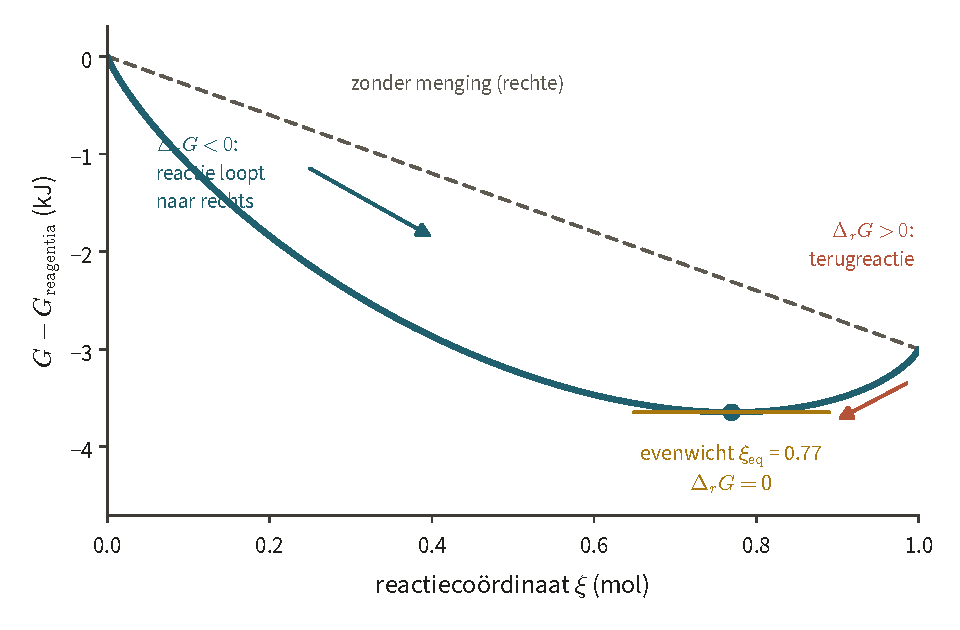
\includegraphics[width=0.7\linewidth]{Figuren/g_reactiecoordinaat}
    \caption{Gibbs-vrije energie van een ideaal gasmengsel $\mathrm{A}\rightleftharpoons\mathrm{B}$ ($\Delta_rG^\circ=\SI{-3}{\kilo\joule\per\mole}$, \SI{298}{\kelvin}) in functie van de reactiecoördinaat $\xi$. Zonder menging zou $G$ lineair dalen tot zuiver B (stippellijn); de mengentropie trekt de curve omlaag en legt het minimum bij $\xi_{\text{eq}}=0.77$, waar de raaklijn horizontaal is ($\Delta_rG=\partial G/\partial\xi=0$). Links ervan verloopt de reactie spontaan naar rechts, rechts ervan verloopt de terugreactie.}
    \label{fig:G-reactiecoordinaat}
\end{figure}

\subsection{Standaardtoestanden per fase}
\label{sec:standaardtoestanden-reagerend}

We schrijven elke chemische potentiaal als $\mu_i = \mu_i^\circ + RT \ln a_i$ (hoofdstuk~\ref{ch:niet-reagerend}, \S~\ref{sec:activiteit}). De standaardtoestand, en dus de vorm van $a_i$, hangt af van de fase:
\begin{itemize}
\item \textbf{gas}: ideaal gas bij $p^\circ = \SI{1}{\bar}$, dus $a_i \approx p_i/p^\circ = y_i P/p^\circ$;
\item \textbf{zuivere vloeistof of vaste stof}: de zuivere stof, dus $a_i \approx 1$;
\item \textbf{opgeloste stof}: een ideale oplossing van $c^\circ = \SI{1}{\mole\per\litre}$, dus $a_i = \gamma_i\,c_i/c^\circ$.
\end{itemize}
Voor een opgeloste stof is de verdunde oplossing de natuurlijke referentie (de logica van Henry, \S~\ref{sec:henry}); voor een zuivere fase de zuivere stof (Raoult). Dat zuivere vaste stoffen en vloeistoffen $a = 1$ hebben, vereenvoudigt heterogene evenwichten sterk (\S~\ref{sec:heterogene-evenwichten}).

\subsection{Het reactiequoti\"ent en de evenwichtsconstante}
\label{sec:evenwichtsconstante-reagerend}\label{sec:evenwichtsconstante}

Vul $\mu_i = \mu_i^\circ + RT \ln a_i$ in in vergelijking~\eqref{eq:delta-r-G}:
\begin{equation}
\Delta_r G = \Delta_r G^\circ + RT \ln Q,
\qquad
\Delta_r G^\circ = \sum_i \nu_i \mu_i^\circ,
\qquad
Q = \prod_i a_i^{\nu_i}.
\end{equation}
$\Delta_r G^\circ$ hangt enkel van de temperatuur af; het \emph{reactiequoti\"ent} $Q$ verandert terwijl de reactie loopt. In evenwicht is $\Delta_r G = 0$ en $Q = K$:
\begin{equation}
\boxed{\;\Delta_r G^\circ = -RT \ln K\;}
\label{eq:K-uit-drG}
\end{equation}
Zo kan je ook schrijven $\Delta_rG = RT\ln(Q/K)$: zolang $Q < K$ loopt de reactie vooruit, bij $Q > K$ achteruit. Elke \SI{5.7}{\kilo\joule\per\mole} in $\Delta_rG^\circ$ verschuift $K$ bij \SI{298}{\kelvin} met een factor tien.

\subsection{Berekening van $\Delta_rG^\circ$ en $K$ uit tabelwaarden}
\label{sec:drG-uit-tabellen}

Er zijn twee equivalente routes, net als voor $\Delta_rH^\circ$ (hoofdstuk~\ref{ch:energie}):
\begin{equation}
\Delta_r G^\circ = \sum_i \nu_i\,\Delta_fG_i^\circ
\qquad\text{of}\qquad
\Delta_rG^\circ = \Delta_rH^\circ - T\,\Delta_rS^\circ,
\end{equation}
met $\Delta_fG^\circ$ de \emph{standaardvormings-Gibbsenergie} (nul voor elementen in hun standaardtoestand).

\begin{voorbeeld}{$K$ voor de ammoniaksynthese bij \SI{298}{\kelvin}}
Route 1: $\Delta_fG^\circ(\mathrm{NH_3,g}) = \SI{-16.4}{\kilo\joule\per\mole}$, dus $\Delta_rG^\circ = 2(-16.4) = \SI{-32.8}{\kilo\joule\per\mole}$.

Route 2: $\Delta_rG^\circ = -92\,000 - 298.15 \times (-198.1) = \SI{-32.9}{\kilo\joule\per\mole}$ ($\Delta_rS^\circ$ uit hoofdstuk~\ref{ch:spontaniteit}, \S~\ref{sec:derde-hoofdwet}).

Beide routes geven hetzelfde, zoals het hoort. Dan is
\[
\ln K = -\frac{-32\,900}{8.314 \times 298.15} = 13.3 \quad\Rightarrow\quad K \approx 6\times10^{5}.
\]
Bij kamertemperatuur is ammoniak dus sterk bevoordeeld. Waarom dan toch \SI{450}{\celsius}? Zie verder.
\end{voorbeeld}

\subsection{Invloed van de temperatuur: de vergelijking van Van 't Hoff}
\label{sec:vanthoff}\label{sec:vanthoff-reagerend}

Hoe $K$ met $T$ verandert, volgt uit de \emph{Gibbs--Helmholtzvergelijking}. Met $(\partial G/\partial T)_p = -S$ (vergelijking~\eqref{eq:fundG}) en $G = H - TS$ geeft de quoti\"entregel
\begin{equation}
\left(\frac{\partial (G/T)}{\partial T}\right)_p = -\frac{S}{T} - \frac{G}{T^2} = -\frac{H}{T^2}.
\label{eq:gibbs-helmholtz}
\end{equation}
Pas dit toe op $\Delta_rG^\circ/T = -R\ln K$, en je krijgt de \emph{vergelijking van Van 't Hoff}:
\begin{gather}
\frac{\dd{\ln K}}{\dd T} = \frac{\Delta_r H^\circ}{RT^2}
\label{eq:vanthoff-diff}\\
\boxed{\;\ln\frac{K_2}{K_1} = -\frac{\Delta_rH^\circ}{R}\left(\frac{1}{T_2}-\frac{1}{T_1}\right)\;}
\label{eq:vanthoff-int}
\end{gather}
De tweede vorm veronderstelt $\Delta_rH^\circ$ constant. Een exotherme reactie verliest dus $K$ bij opwarmen, een endotherme wint. Figuur~\ref{fig:K-temperatuur} toont dat voor vijf industri\"ele reacties: wie de grafiek kent, weet meteen waarom stoomreforming heet moet en waarom de SO$_3$-reactor gekoeld wordt.

\begin{figure}[htb]
    \centering
    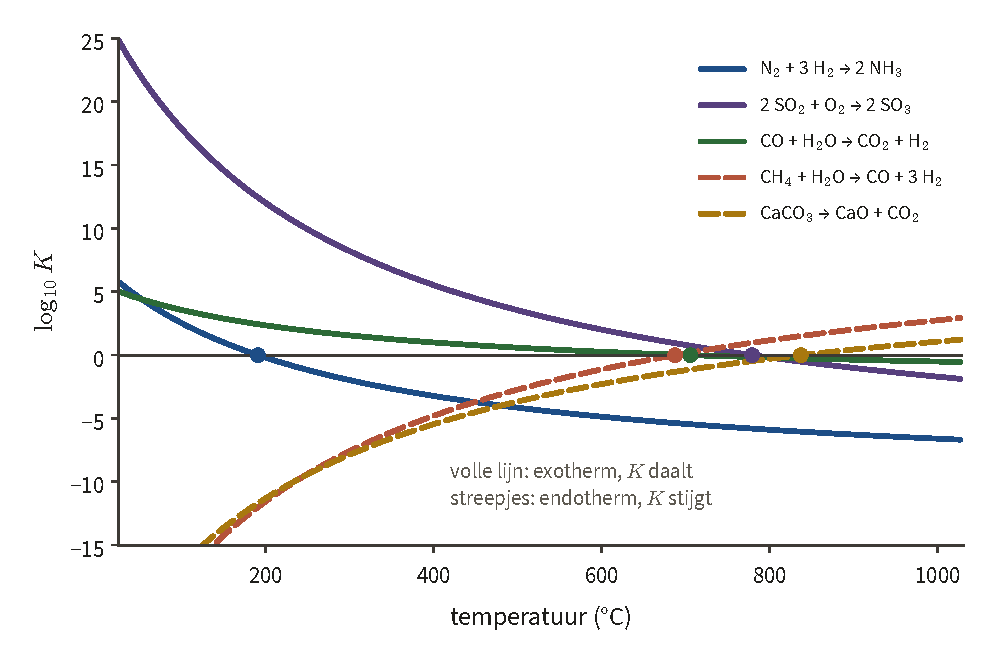
\includegraphics[width=0.75\linewidth]{Figuren/K_temperatuur}
    \caption{Evenwichtsconstante van vijf industri\"ele reacties in functie van de temperatuur, berekend met $\Delta_rH^\circ$ en $\Delta_rS^\circ$ bij \SI{298}{\kelvin} (constant verondersteld; bron: NIST WebBook). Het punt op de horizontale lijn $K = 1$ ligt bij $T = \Delta_rH^\circ/\Delta_rS^\circ$. Exotherme reacties (volle lijn) worden ongunstiger bij hoge $T$, endotherme (streepjes) gunstiger.}
    \label{fig:K-temperatuur}
\end{figure}

\begin{voorbeeld}{Ammoniak bij \SI{700}{\kelvin}}
Met $K_1 = 6\times10^5$ bij \SI{298.15}{\kelvin}:
\[
\ln\frac{K_2}{K_1} = \frac{92\,000}{8.314}\left(\frac{1}{700}-\frac{1}{298.15}\right) = -21.3
\quad\Rightarrow\quad K_2 \approx 3\times10^{-4}.
\]
Tien grootteordes minder (figuur~\ref{fig:vanthoff}). Bij \SI{700}{\kelvin} is de reactie thermodynamisch ongunstig. Dat men toch zo warm werkt, is een keuze voor snelheid (hoofdstuk~\ref{ch:kinetiek}); de hoge druk moet de opbrengst terugwinnen (\S~\ref{sec:ice-tabel}).
\end{voorbeeld}

\begin{figure}[htb]
    \centering
    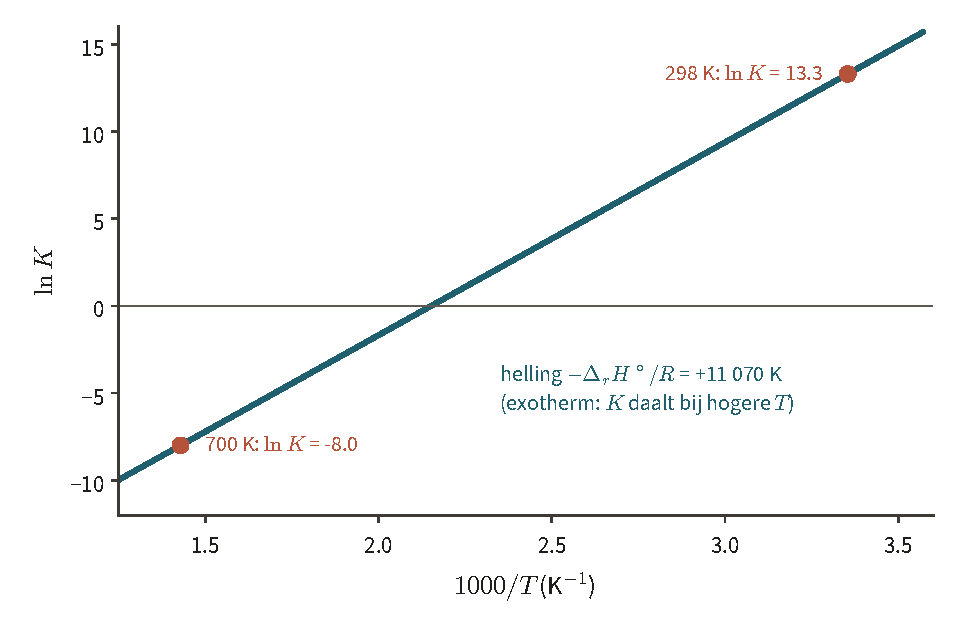
\includegraphics[width=0.65\linewidth]{Figuren/vanthoff_ammoniak}
    \caption{Van 't Hoff-diagram voor de ammoniaksynthese, met $\Delta_rH^\circ=\SI{-92}{\kilo\joule\per\mole}$ constant verondersteld en de twee punten uit het voorbeeld. Omdat de reactie exotherm is, stijgt $\ln K$ met $1/T$: de evenwichtsconstante daalt bij hogere temperatuur. De helling is $-\Delta_rH^\circ/R$ (vergelijking~\eqref{eq:vanthoff-int}).}
    \label{fig:vanthoff}
\end{figure}

\subsection{Verband tussen $K_p$, $K_c$ en $K_x$}
\label{sec:Kp-Kc-Kx}

Voor gasreacties kan je $K$ uitdrukken met parti\"ele drukken ($K_p$), concentraties ($K_c$) of molfracties ($K_x$). Met $p_i = y_i P = c_i RT$ voor ideale gassen:
\begin{equation}
K_p = K_c \left(\frac{RT}{p^\circ}\right)^{\Delta \nu} = K_x \left(\frac{P}{p^\circ}\right)^{\Delta \nu},
\label{eq:Kp-Kc-Kx-relatie}
\end{equation}
met $\Delta \nu$ de verandering van het aantal mol gas. $K_p$ en $K_c$ hangen enkel van $T$ af, $K_x$ ook van de totale druk. Voor ammoniak is $\Delta\nu = -2$, dus $K_x = K_p (P/p^\circ)^2$: honderd keer meer druk geeft $K_x$ tienduizend keer groter. Zo duwt druk het evenwicht naar ammoniak zonder $K_p$ te veranderen.

\section{Het chemisch evenwicht kwantitatief berekenen}

\subsection{Numerieke evenwichtsberekening met reactietabel (ICE-table)}
\label{sec:ice-tabel}

Het werkpaard van de ingenieur is de \emph{reactietabel} (ICE: Initial, Change, Equilibrium). Alle molhoeveelheden worden uitgedrukt in \'e\'en onbekende, $\xi$. Voor ammoniak met een stoichiometrische voeding:

\begin{center}
\begin{tabular}{lcccc}
\toprule
 & $\mathrm{N_2}$ & $\mathrm{H_2}$ & $\mathrm{NH_3}$ & totaal \\
\midrule
Initieel (mol) & 1 & 3 & 0 & 4 \\
Verandering (mol) & $-\xi$ & $-3\xi$ & $+2\xi$ & $-2\xi$ \\
Evenwicht (mol) & $1-\xi$ & $3-3\xi$ & $2\xi$ & $4-2\xi$ \\
\bottomrule
\end{tabular}
\end{center}
Met $p_i = y_i P$ en $y_i = n_i/n_\text{tot}$ wordt $K_p$ een functie van $\xi$ alleen, op te lossen met Doelzoeken in Excel.

\begin{voorbeeld}{Ammoniak bij \SI{700}{\kelvin} en \SI{100}{\bar}}
Met $K_p \approx 3\times10^{-4}$ (\S~\ref{sec:vanthoff}):
\[
K_p = \frac{\left(\dfrac{2\xi}{4-2\xi}\right)^2}{\left(\dfrac{1-\xi}{4-2\xi}\right)\left(\dfrac{3-3\xi}{4-2\xi}\right)^3}\left(\frac{P}{p^\circ}\right)^{-2} = 3\times10^{-4}
\quad\Rightarrow\quad \xi \approx 0.445.
\]
Het evenwichtsmengsel bevat $y_{\mathrm{NH_3}} = 0.891/3.109 = \SI{28.6}{\percent}$ ammoniak, en \SI{44.5}{\percent} van de stikstof is omgezet. Herhaal je dat voor andere drukken, dan krijg je figuur~\ref{fig:nh3-vs-druk}: bij \SI{1}{\bar} amper \SI{0.6}{\percent}, bij \SI{300}{\bar} bijna de helft.
\end{voorbeeld}

\begin{figure}[htb]
    \centering
    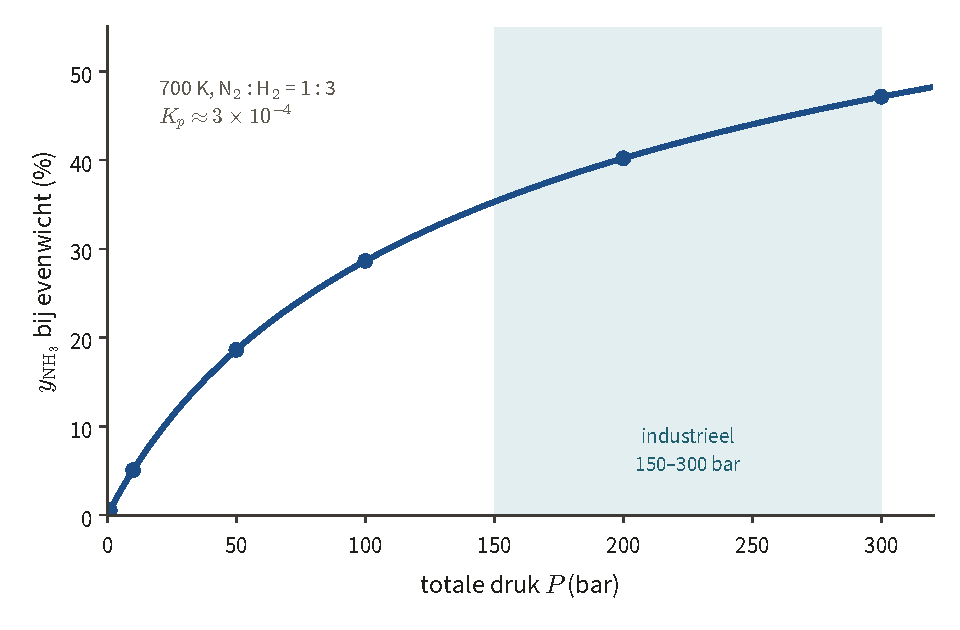
\includegraphics[width=0.7\linewidth]{Figuren/nh3_druk}
    \caption{Evenwichtsmolfractie ammoniak bij \SI{700}{\kelvin} in functie van de totale druk, voor een stoichiometrische voeding, berekend met de reactietabel. De opbrengst stijgt eerst snel en vlakt daarna af; de band toont het industri\"ele drukbereik.}
    \label{fig:nh3-vs-druk}
\end{figure}

\section{Factoren die het evenwicht be\"invloeden}

\subsection{Invloed van druk en inerte gassen}
\label{sec:druk-inerte-gassen}

\textbf{Druk} verandert $K_p$ niet, maar wel $K_x = K_p (P/p^\circ)^{-\Delta\nu}$ (\S~\ref{sec:Kp-Kc-Kx}). Bij $\Delta\nu < 0$ (ammoniak, methanol) helpt druk, bij $\Delta\nu > 0$ (stoomreforming) werkt ze tegen, bij $\Delta\nu = 0$ (watergasshift) maakt ze niets uit.

\textbf{Inerte gassen} (argon en methaan in de ammoniaklus) doen bij constante totale druk hetzelfde als een lagere druk: ze verdunnen de reagentia. Bij $\Delta\nu < 0$ daalt de opbrengst. Daarom spuit men in een recyclelus voortdurend een kleine \emph{purge} af, anders stapelen de inerten zich op (\S~\ref{sec:haber-bosch-integraal}).

\subsection{Het principe van Le Ch\^atelier}
\label{sec:le-chatelier-reagerend}\label{sec:le-chatelier}

Een verstoord evenwicht verschuift zo dat de verstoring deels wordt tegengewerkt:
opwarmen bevoordeelt de endotherme richting; druk verhogen de kant met minder mol gas; een product wegnemen of een reagens toevoegen bevoordeelt de producten. Dat is geen extra natuurwet: de verstoring verandert $G$ van alle toestanden, en het minimum schuift op. Van 't Hoff en $K_x$ maken het kwantitatief.

\subsection{Heterogene evenwichten}
\label{sec:heterogene-evenwichten}

Zuivere vaste stoffen en vloeistoffen hebben $a \approx 1$ en verdwijnen uit $K$.

\begin{voorbeeld}{Ontleding van kalksteen}
Voor $\mathrm{CaCO_3(s) \rightleftharpoons CaO(s) + CO_2(g)}$ is $K = p_{\mathrm{CO_2}}/p^\circ$. Bij elke temperatuur hoort dus \'e\'en evenwichtsdruk van \ce{CO2}, ongeacht hoeveel kalk er ligt: bij \SI{800}{\celsius} ongeveer \SI{0.22}{\bar}. Een kalkoven werkt alleen als de \ce{CO2}-druk boven de kalk lager blijft; daarom blaast men er rookgas of lucht door.
\end{voorbeeld}

Hetzelfde geldt voor het oplossen van een zout: voor $\mathrm{AgCl(s) \rightleftharpoons Ag^+ + Cl^-}$ is $K_{ps} = a_{\mathrm{Ag^+}}a_{\mathrm{Cl^-}} = 1.8\times10^{-10}$ bij \SI{25}{\celsius}, zodat $s = \sqrt{K_{ps}} = \SI{1.3e-5}{\mole\per\litre}$ (meer hierover in Analytische chemie).

\subsection{Gekoppelde reacties en simultane evenwichten}
\label{sec:gekoppelde-reacties}

Vaak lopen meerdere reacties tegelijk, met gemeenschappelijke componenten. Dan moet het mengsel aan elke evenwichtsvoorwaarde tegelijk voldoen, met een reactie-uitbreiding $\xi_1$, $\xi_2$, \ldots\ per reactie. Dat is de ICE-methode met meer onbekenden; in de praktijk lost een processimulator dit op. Het belangrijkste voorbeeld is de productie van waterstof.

\subsection{Tweede case: waterstof uit aardgas}
\label{sec:case-waterstof}

De waterstof voor ammoniak komt grotendeels uit aardgas, via twee gekoppelde evenwichten met een tegengesteld karakter (figuur~\ref{fig:K-temperatuur}).

\paragraph{Stoomreforming: endotherm, dus heet.}
\[
\ce{CH4 + H2O <=> CO + 3 H2}, \qquad \Delta_r H^\circ = \SI{+206}{\kilo\joule\per\mole},\quad \Delta\nu = +2.
\]
Hoge temperatuur en lage druk zijn gunstig. Men werkt bij \SIrange{800}{900}{\celsius} in buizen met nikkelkatalysator, van buitenaf verwarmd in een oven. De druk is toch \SIrange{20}{30}{\bar}: de rest van de installatie werkt onder druk, en een compacte reactor is goedkoper, ook al kost dat wat omzetting.

\paragraph{Watergasshift: exotherm, dus in twee trappen.}
\[
\ce{CO + H2O <=> CO2 + H2}, \qquad \Delta_r H^\circ = \SI{-41.2}{\kilo\joule\per\mole},\quad \Delta_r S^\circ = \SI{-42.1}{\joule\per\mole\per\kelvin},\quad \Delta\nu = 0.
\]

\begin{voorbeeld}{Watergasshift bij 400 en \SI{200}{\celsius}}
Voeding: 1 mol \ce{CO} en 2 mol \ce{H2O}. Bij omzetting $X$ is (druk en totaal aantal mol vallen weg, want $\Delta\nu = 0$):
\[
K = \frac{X^2}{(1-X)(2-X)}.
\]
\textbf{Bij \SI{400}{\celsius}}: $\ln K = 41\,200/(8.314 \times 673) - 42.1/8.314 = 7.36 - 5.06 = 2.30$, dus $K \approx 10$ en $9X^2 - 30X + 20 = 0$ geeft $X = 0.92$.

\textbf{Bij \SI{200}{\celsius}}: $\ln K = 10.48 - 5.06 = 5.41$, dus $K \approx 220$ en $X = 0.995$.

Bij \SI{400}{\celsius} blijft 8\,\% CO over, bij \SI{200}{\celsius} nog 0.5\,\%. Daarom twee shiftreactoren na elkaar: een \emph{hogetemperatuurshift} (\SIrange{350}{450}{\celsius}, ijzer-chroom) die snel het grootste deel omzet, en na tussenkoeling een \emph{lagetemperatuurshift} (\SIrange{200}{250}{\celsius}, koper) die het evenwicht verder duwt. De thermodynamica wil koud, de kinetiek warm: de ingenieur splitst het probleem op.
\end{voorbeeld}

\section{Van thermodynamica naar procesontwerp}

\subsection{Thermodynamische strategie\"en voor procesontwerp}
\label{sec:procesontwerp-strategieen}

De thermodynamica bepaalt de maximale omzetting; het procesontwerp bepaalt hoe dicht je erbij komt. Vier strategie\"en volgen rechtstreeks uit dit hoofdstuk:
\begin{enumerate}
\item \textbf{Temperatuur en druk kiezen} met Van 't Hoff en $K_x$.
\item \textbf{Product verwijderen}: houdt $Q < K$, zodat de reactie blijft lopen zonder dat $K$ verandert. Ammoniak wordt na afkoeling gecondenseerd; bij een verestering haalt men het water weg.
\item \textbf{Recycleren}: wat per doorgang niet reageert (bij ammoniak meer dan de helft), wordt na scheiding teruggestuurd, met een purge voor de inerten.
\item \textbf{Reactie en scheiding integreren}: reactieve destillatie, membraanreactoren. Het product verdwijnt al tijdens de reactie.
\end{enumerate}

\subsection{Evenwicht en warmte samen: de adiabatische reactor}
\label{sec:adiabatische-evenwichtsreactor}

In een adiabatische reactor warmt een exotherme reactie het mengsel op: $T = T_\mathrm{in} + \Delta T_\mathrm{ad}\,X$ (hoofdstuk~\ref{ch:energie}, \S~\ref{sec:warmte-effecten}). Bij een evenwichtsreactie is dat vervelend: hoe meer omzetting, hoe warmer, hoe lager de evenwichtsomzetting. De reactie stopt waar de rechte van de energiebalans de evenwichtscurve snijdt.

Figuur~\ref{fig:so2-bedden} toont dat voor $\ce{SO2 + 1/2 O2 <=> SO3}$ ($\Delta_r H^\circ = \SI{-98.9}{\kilo\joule\per\mole}$) in een zwavelzuurfabriek, met 10\,\% \ce{SO2}, 11\,\% \ce{O2} en 79\,\% \ce{N2}. Met een gemiddelde $C_p = \SI{32}{\joule\per\mole\per\kelvin}$ is $\Delta T_\mathrm{ad} = 0.10 \times 98\,900/32 \approx \SI{310}{\kelvin}$ bij volledige omzetting.

\begin{figure}[htb]
    \centering
    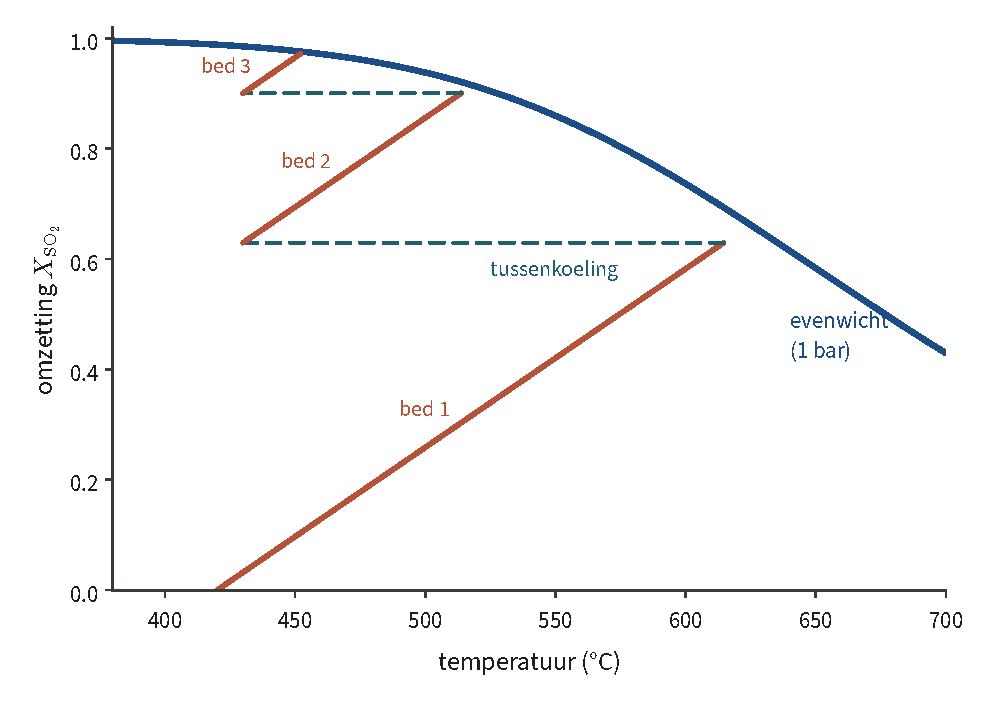
\includegraphics[width=0.75\linewidth]{Figuren/so2_bedden}
    \caption{Evenwichtsomzetting van \ce{SO2} naar \ce{SO3} (blauw) en drie adiabatische katalysatorbedden met tussenkoeling tot \SI{430}{\celsius} (rood). In elk bed stijgen omzetting en temperatuur samen langs een rechte, tot dicht bij het evenwicht. Berekend met $\Delta_r H^\circ$ en $\Delta_r S^\circ$ uit tabellen (NIST) en een gemiddelde $C_p$.}
    \label{fig:so2-bedden}
\end{figure}

Het eerste bed start bij \SI{420}{\celsius} (kouder werkt de vanadiumkatalysator niet) en loopt op tot ongeveer \SI{615}{\celsius} bij 63\,\% omzetting. Na afkoeling tot \SI{430}{\celsius} brengt een tweede bed de omzetting naar 90\,\%, een derde naar 97\,\%. Moderne installaties absorberen dan het \ce{SO3} en sturen het restgas door een vierde bed (\emph{dubbele absorptie}): product weg, $Q$ omlaag, meer dan 99.7\,\%. Met de warmte uit de tussenkoelers maakt men stoom: een zwavelzuurfabriek levert netto energie.

\subsection{Ge\"integreerde casestudy: de synthese van ammoniak}
\label{sec:haber-bosch-integraal}

We kunnen nu de drie vragen uit \S~\ref{sec:haber-bosch} beantwoorden (figuur~\ref{fig:haber-bosch-schema}).

\begin{figure}[htb]
    \centering
    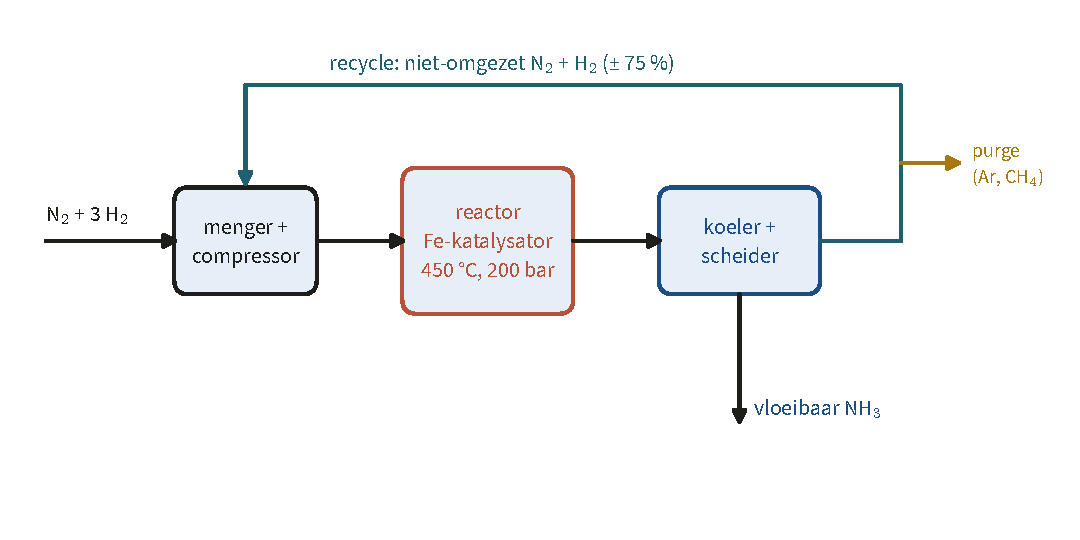
\includegraphics[width=0.85\linewidth]{Figuren/haber_bosch_schema}
    \caption{Vereenvoudigd blokschema van de Haber--Boschlus. Per doorgang wordt slechts een deel van \ce{N2} en \ce{H2} omgezet; na afkoeling condenseert \ce{NH3} en wordt het afgescheiden. De rest gaat terug naar de reactor (recycle), met een kleine purge om inerte gassen af te voeren.}
    \label{fig:haber-bosch-schema}
\end{figure}

\begin{itemize}
\item \textbf{Waarom stopt de reactie halfweg?} Het minimum van $G$ ligt tussen reagentia en producten (figuur~\ref{fig:G-reactiecoordinaat}).
\item \textbf{Waarom \SI{450}{\celsius}?} Bij kamertemperatuur is $K = 6\times10^5$, maar de $\mathrm{N{\equiv}N}$-binding maakt de reactie veel te traag. Warmer gaat sneller, maar $K$ daalt tot $3\times10^{-4}$ bij \SI{700}{\kelvin}. Een ijzerkatalysator verlaagt de nodige temperatuur, zonder $K$ te veranderen (hoofdstuk~\ref{ch:kinetiek}).
\item \textbf{Waarom \SIrange{150}{300}{\bar}?} Omdat $\Delta\nu = -2$: druk wint de opbrengst terug die de temperatuur kost (figuur~\ref{fig:nh3-vs-druk}).
\item \textbf{Hoeveel ammoniak?} Per doorgang zet men minder dan de helft om. Ammoniak condenseren en het restgas recycleren (met purge) brengt de globale omzetting toch boven \SI{95}{\percent}.
\end{itemize}

\begin{besluit}{Thermodynamica bepaalt, kinetiek levert}
De thermodynamica legt de grens vast; het werkpunt van een installatie is een compromis tussen evenwicht, snelheid, energie, investering en veiligheid.
\end{besluit}

\section{Samenvatting en reflectie}

Het criterium van hoofdstuk~\ref{ch:spontaniteit}, een minimale Gibbs-vrije energie, bepaalt ook waar een chemische reactie stopt. In hoofdstuk~\ref{ch:elektrochemie} breiden we dit uit naar systemen waarin naast de chemische potentiaal ook de elektrische potentiaal een rol speelt: batterijen, brandstofcellen, elektrolysers en corrosie.

\begin{samenvatting}{Thermodynamisch evenwicht van reagerende systemen}
\begin{itemize}
\item De reactie-Gibbsenergie $\Delta_rG=\sum_i\nu_i\mu_i$ is de helling van $G$ langs de reactieco\"ordinaat $\xi$; evenwicht ligt in het minimum, waar $\Delta_rG=0$.
\item Met $\mu_i=\mu_i^\circ+RT\ln a_i$ volgt $\Delta_rG=\Delta_rG^\circ+RT\ln Q$ en in evenwicht $\Delta_rG^\circ=-RT\ln K$. $Q<K$: de reactie loopt vooruit.
\item $\Delta_rG^\circ$ volgt uit tabellen: $\sum_i\nu_i\Delta_fG_i^\circ$ of $\Delta_rH^\circ-T\Delta_rS^\circ$.
\item Van 't Hoff: $\dd\ln K/\dd T=\Delta_rH^\circ/RT^2$. Exotherme reacties verliezen opbrengst bij hogere temperatuur.
\item $K_p$ en $K_c$ hangen enkel van $T$ af; $K_x=K_p(P/p^\circ)^{-\Delta\nu}$ hangt ook van de druk af. Inerte gassen verlagen bij constante druk de opbrengst van reacties met $\Delta\nu<0$.
\item De evenwichtssamenstelling volgt uit een reactietabel en \'e\'en vergelijking in $\xi$ (of meerdere, bij gekoppelde reacties).
\item Zuivere vaste stoffen en vloeistoffen hebben activiteit 1 en verschijnen niet in $K$.
\item In een adiabatische reactor stijgt de temperatuur met de omzetting (werklijn) tot ze de evenwichtscurve snijdt. Bij exotherme evenwichtsreacties (SO$_2$-oxidatie, watergasshift) werkt men daarom met meerdere bedden en tussenkoeling: eerst snelheid bij hoge $T$, dan opbrengst bij lage $T$.
\item Ontwerpstrategie\"en: $T$ en $P$ kiezen, product verwijderen, recycleren met purge, reactie en scheiding integreren. Thermodynamica bepaalt de grens, kinetiek en economie het werkpunt.
\end{itemize}
\end{samenvatting}

\begin{reflectie}{Thermodynamisch evenwicht van reagerende systemen}
\begin{enumerate}
\item Waarom stopt een reactie in een gesloten vat meestal v\'o\'or alle reagentia op zijn, ook als $\Delta_rG^\circ$ sterk negatief is?
\item Een katalysator verlaagt de activeringsenergie. Waarom verandert hij $K$ niet?
\item Waarom heeft een drukverhoging geen invloed op $K_p$, maar wel op de opbrengst van ammoniak?
\item Bij de ammoniaksynthese daalt $K$ met tien grootteordes tussen \SI{298}{\kelvin} en \SI{700}{\kelvin}. Waarom werkt men toch bij \SI{700}{\kelvin}?
\item Waarom haalt een groter adiabatisch katalysatorbed niet altijd een hogere omzetting?
\item Wat gebeurt er met de reactorcapaciteit als je de purge in de Haber--Boschlus dichtdraait?
\item Een kalkoven werkt bij atmosferische druk. Waarom blaast men lucht of rookgas door de oven?
\item Geef een voorbeeld van een proces waarin reactie en scheiding in \'e\'en toestel gebeuren, en leg uit waarom dat de omzetting verhoogt.
\end{enumerate}
\end{reflectie}

\newpage
\section{Oefeningen}

% Oefeningen bij dit hoofdstuk (ingevoegd achteraan het hoofdstuk met \input).
% Een oefening:  \begin{oefening}[titel] ... \end{oefening}   (boek en website)
% De oplossing:  \begin{oplossing} ... \end{oplossing}       (enkel website, dichtgeklapt)

Neem $R = \SI{8.314}{\joule\per\mole\per\kelvin}$, $p^\circ = \SI{1}{\bar}$ en $c^\circ = \SI{1}{\mole\per\litre}$; gassen zijn ideaal.

\begin{oefening}[Evenwichtsconstante en standaardreactie-Gibbsenergie]
Voor de reactie

\[
\mathrm{N_2O_4(g) \rightleftharpoons 2\,NO_2(g)}
\]

bedraagt \(\Delta_r G^\circ = +4.8\,\mathrm{kJ/mol}\) bij \(298\,\mathrm{K}\).

\begin{enumerate}
\item[(a)]
  Bereken de evenwichtsconstante \(K\) bij \(298\,\mathrm{K}\).
\item[(b)]
  Is de reactie bij standaardomstandigheden spontaan in de voorwaartse richting?
\item[(c)]
  Bij welke waarde van het reactiequotiënt \(Q\) zou de reactie precies in evenwicht zijn?
\end{enumerate}
\end{oefening}
\begin{oplossing}
\textbf{Resultaat:} (a) \(K\) = \textbf{0.144}. (b) \textbf{Nee}, bij \(Q = 1\) verloopt de reactie naar links. (c) Evenwicht bij \(Q = K\) = \textbf{0.144}.

\textbf{(a)} \(K = \exp(-\Delta_r G^\circ/RT) = \exp\!\left(-\dfrac{4800}{(8.314)(298)}\right) = 0.144\).

\textbf{(b)} Nee. Bij standaardomstandigheden (beide gassen bij \(1\,\mathrm{bar}\), dus \(Q = 1\)) is \(\Delta_r G = \Delta_r G^\circ > 0\): de reactie verloopt spontaan in de \emph{omgekeerde} richting tot het evenwicht bereikt is. Dat betekent niet dat er geen \(\mathrm{NO_2}\) gevormd wordt: vertrekkend van zuiver \(\mathrm{N_2O_4}\) (\(Q = 0\)) dissocieert een deel wel degelijk.

\textbf{(c)} Evenwicht wanneer \(\Delta_r G = \Delta_r G^\circ + RT\ln Q = 0\), dus \(Q = K = 0.144\).
\end{oplossing}

\begin{oefening}[Invloed van temperatuur: de vergelijking van Van 't Hoff]
Voor de ammoniaksynthese \(\mathrm{N_2 + 3\,H_2 \rightleftharpoons 2\,NH_3}\) bedraagt \(\Delta_r H^\circ = -92.4\,\mathrm{kJ/mol}\) en \(\Delta_r G^\circ = -33.0\,\mathrm{kJ/mol}\) bij \(298\,\mathrm{K}\).

\begin{enumerate}
\item[(a)]
  Bereken \(K\) bij \(298\,\mathrm{K}\).
\item[(b)]
  Schat \(K\) bij \(700\,\mathrm{K}\) (veronderstel \(\Delta_r H^\circ\) constant). Gebruik de geïntegreerde vorm van Van 't Hoff.
\item[(c)]
  Verklaar vanuit het teken van \(\Delta_r H^\circ\) waarom de evenwichtsconstante daalt bij stijgende temperatuur.
\item[(d)]
  Combineer met Hoofdstuk 1: bereken ook \(\Delta_r S^\circ\) bij \(298\,\mathrm{K}\).
\end{enumerate}
\end{oefening}
\begin{oplossing}
\textbf{Resultaat:} (a) \(K_{298}\) = \textbf{6.1\ensuremath{\cdot{}}10\ensuremath{^{5}}}. (b) \(K_{700}\) = \textbf{3.0\ensuremath{\cdot{}}10\ensuremath{^{-4}}}. (c) Exotherm: \(K\) \textbf{daalt} met \(T\). (d) \(\Delta_r S^\circ\) = \textbf{\ensuremath{-}199 J/(mol\ensuremath{\cdot{}}K)}.

\textbf{(a)} \(\ln K = 33\,000/(8.314 \times 298) = 13.32\), dus \(K = 6.1\times10^{5}\).

\textbf{(b)}

\[
\ln\frac{K_2}{K_1} = -\frac{-92\,400}{8.314}\left(\frac{1}{700} - \frac{1}{298}\right) = -21.4
\]

zodat \(\ln K_2 = 13.32 - 21.4 = -8.1\) en \(K_2 = 3.0\times10^{-4}\).

\textbf{(c)} Volgens \(\mathrm{d}\ln K/\mathrm{d}T = \Delta_r H^\circ/(RT^2)\) daalt \(\ln K\) met \(T\) wanneer \(\Delta_r H^\circ < 0\). Fysisch: bij een exotherme reactie ``werkt'' extra warmte de vorming van producten tegen (Le Chatelier).

\textbf{(d)} \(\Delta_r S^\circ = (\Delta_r H^\circ - \Delta_r G^\circ)/T = (-92\,400 + 33\,000)/298 = -199\,\mathrm{J/(mol\cdot K)}\), in overeenstemming met de \(-198.1\,\mathrm{J/(mol\cdot K)}\) uit de theorie. Negatief, omdat 4 mol gas omgezet wordt in 2 mol gas.
\end{oplossing}

\begin{oefening}[Le Châtelier: invloed van druk op ammoniaksynthese]
Beschouw opnieuw de ammoniaksynthese. Bij een bepaalde temperatuur bedraagt \(K = 1.0\times10^{-3}\).

\begin{enumerate}
\item[(a)]
  Een reactiemengsel bevat aanvankelijk gelijke molfracties \(\mathrm{N_2}\), \(\mathrm{H_2}\) en \(\mathrm{NH_3}\) bij een totale druk van \(1\,\mathrm{bar}\). Bereken \(Q\) en bepaal de spontane richting.
\item[(b)]
  Hoe verandert \(Q\) wanneer de totale druk wordt verhoogd tot \(200\,\mathrm{bar}\)? Verklaar waarom een drukverhoging de vorming van ammoniak bevordert.
\item[(c)]
  Waarom verandert de evenwichtsconstante \(K\) zelf \emph{niet} met de druk?
\end{enumerate}

\emph{Hint:} bij een gasreactie met afname van aantal mol geldt \(Q \propto p^{\Delta \nu} = 1/p^{|\Delta \nu|}\).
\end{oefening}
\begin{oplossing}
\textbf{Resultaat:} (a) \(Q\) = \textbf{9} \textgreater{} \(K\): ammoniak ontleedt. (b) \(Q\) = \textbf{2.25\ensuremath{\cdot{}}10\ensuremath{^{-4}}} \textless{} \(K\): ammoniak wordt gevormd. (c) \(K\) hangt enkel af van \(T\).

\textbf{(a)} Met \(p_i = x_i p\) en \(p^\circ = 1\,\mathrm{bar}\):

\[
Q = \frac{(x_{\mathrm{NH_3}}p/p^\circ)^2}{(x_{\mathrm{N_2}}p/p^\circ)(x_{\mathrm{H_2}}p/p^\circ)^3} = \frac{x_{\mathrm{NH_3}}^2}{x_{\mathrm{N_2}}x_{\mathrm{H_2}}^3}\left(\frac{p}{p^\circ}\right)^{-2} = \frac{(1/3)^2}{(1/3)^4}(1)^{-2} = 9
\]

\(Q = 9 \gg K\): de reactie verloopt spontaan naar links, ammoniak ontleedt.

\textbf{(b)} De samenstelling blijft dezelfde, maar de drukfactor wordt \((200)^{-2}\): \(Q = 9/40\,000 = 2.25\times10^{-4} < K\). Nu verloopt de reactie spontaan naar rechts. Omdat het aantal mol gas afneemt (\(\Delta\nu = 2 - 4 = -2\)), daalt \(Q\) met de druk als \(p^{\Delta\nu} = p^{-2}\); het evenwicht moet dan naar de kant van de producten schuiven om \(Q\) weer gelijk te maken aan \(K\).

\textbf{(c)} \(K = \exp(-\Delta_r G^\circ/RT)\) is gedefinieerd met de standaardtoestand bij de vaste druk \(p^\circ = 1\,\mathrm{bar}\). Daardoor hangt \(K\) enkel af van de temperatuur. De druk verandert wel \(Q\), en dus de evenwichtssamenstelling.
\end{oplossing}

\begin{oefening}[\(K_p\), \(K_c\) en \(K_x\) voor de ammoniaksynthese]
Voor \(\mathrm{N_2 + 3\,H_2 \rightleftharpoons 2\,NH_3}\) geldt \(K_p \approx 3\times10^{-4}\) bij \(700\,\mathrm{K}\).

\begin{enumerate}
\item[(a)]
  Bereken \(K_c\) bij \(700\,\mathrm{K}\). Let op de eenheden: gebruik \(c^\circ = 1\,\mathrm{mol/L} = 1000\,\mathrm{mol/m^3}\).
\item[(b)]
  Bereken \(K_x\) bij \(1\,\mathrm{bar}\) en bij \(200\,\mathrm{bar}\).
\item[(c)]
  Welke van de drie constanten verandert wanneer je de reactor bij dezelfde temperatuur op een hogere druk zet? Waarom is \(K_c \neq K_p\)?
\end{enumerate}
\end{oefening}
\begin{oplossing}
\textbf{Resultaat:} (a) \(K_c\) \ensuremath{\approx{}} \textbf{1.0}. (b) \(K_x\) = \textbf{3\ensuremath{\cdot{}}10\ensuremath{^{-4}}} bij 1 bar en \textbf{12} bij 200 bar. (c) Enkel \textbf{\(K_x\)} verandert met de druk; \(K_c \neq K_p\) omdat \(\Delta\nu = -2 \neq 0\).

\textbf{(a)} Met \(p_i = c_i RT\) geldt \(K_p = K_c\,(c^\circ RT/p^\circ)^{\Delta\nu}\). Hier is

\[
\frac{c^\circ RT}{p^\circ} = \frac{(1000\,\mathrm{mol/m^3})(8.314)(700)}{10^5\,\mathrm{Pa}} = 58.2
\]

en \(\Delta\nu = -2\), dus \(K_c = K_p\,(58.2)^{2} = (3\times10^{-4})(3387) = 1.0\).

\textbf{(b)} \(K_x = K_p\,(P/p^\circ)^{-\Delta\nu} = K_p\,(P/p^\circ)^{2}\): bij \(1\,\mathrm{bar}\) is \(K_x = K_p = 3\times10^{-4}\), bij \(200\,\mathrm{bar}\) is \(K_x = 3\times10^{-4} \times 40\,000 = 12\).

\textbf{(c)} \(K_p\) en \(K_c\) hangen enkel van de temperatuur af; \(K_x\) groeit met \(P^2\), wat de hogere ammoniakfractie bij hoge druk verklaart. \(K_c\) en \(K_p\) verschillen omdat ze naar een andere standaardtoestand verwijzen (\(1\,\mathrm{mol/L}\) tegenover \(1\,\mathrm{bar}\)). Ze zijn enkel gelijk wanneer \(\Delta\nu = 0\), zoals bij de water-gas-shiftreactie.
\end{oplossing}

\begin{oefening}[Inert gas in de ammoniakreactor]
In het voorbeeld van \S~\ref{sec:ice-tabel} werd de evenwichtssamenstelling berekend bij \(700\,\mathrm{K}\) en \(100\,\mathrm{bar}\) (\(K_p \approx 3\times10^{-4}\)), vertrekkend van \(1\,\mathrm{mol}\) \(\mathrm{N_2}\) en \(3\,\mathrm{mol}\) \(\mathrm{H_2}\): \(\xi \approx 0.445\). In een echte installatie stapelt argon (uit de lucht) zich op in de recyclestroom.

\begin{enumerate}
\item[(a)]
  Stel de reactietabel op wanneer de voeding bovendien \(2\,\mathrm{mol}\) argon bevat, bij dezelfde totale druk van \(100\,\mathrm{bar}\).
\item[(b)]
  Bereken de omzetting van stikstof en de molfractie ammoniak. Vergelijk met de situatie zonder argon.
\item[(c)]
  Wat zou er gebeuren als je het argon toevoegt bij constant volume?
\item[(d)]
  Waarom voorziet men een purgestroom in de recyclelus?
\end{enumerate}
\end{oefening}
\begin{oplossing}
\textbf{Resultaat:} (b) \(\xi\) = \textbf{0.354} (35 \% omzetting, tegenover 44.5 \%); \(y_{\mathrm{NH_3}}\) = \textbf{0.134} (tegenover 0.286). (c) Bij constant volume: \textbf{geen effect}. (d) Zonder purge stapelt het inerte gas zich op en daalt de omzetting per doorgang.

\textbf{(a)}

\begin{center}
\begin{tabular}{lllll}
\toprule
 & \(\mathrm{N_2}\) & \(\mathrm{H_2}\) & \(\mathrm{NH_3}\) & Ar \\
\midrule
Initieel (mol) & 1 & 3 & 0 & 2 \\
Verandering (mol) & \(-\xi\) & \(-3\xi\) & \(+2\xi\) & 0 \\
Evenwicht (mol) & \(1-\xi\) & \(3-3\xi\) & \(2\xi\) & 2 \\
\bottomrule
\end{tabular}
\end{center}

met \(n_{\text{tot}} = 6 - 2\xi\).

\textbf{(b)} De evenwichtsvoorwaarde wordt

\[
K_p = \frac{\left(\dfrac{2\xi}{6-2\xi}\right)^2}{\left(\dfrac{1-\xi}{6-2\xi}\right)\left(\dfrac{3-3\xi}{6-2\xi}\right)^3}\left(\frac{P}{p^\circ}\right)^{-2} = 3\times10^{-4}
\]

Numeriek oplossen geeft \(\xi = 0.354\), \(n_{\text{tot}} = 5.29\,\mathrm{mol}\) en \(y_{\mathrm{NH_3}} = 0.708/5.29 = 0.134\). Zonder argon was \(\xi = 0.445\) en \(y_{\mathrm{NH_3}} = 0.286\). Het argon verdunt de reactanten: hun partiële drukken dalen, alsof de reactor bij een lagere druk werkt, en het evenwicht schuift naar de kant met meer mol gas.

\textbf{(c)} Bij constant volume blijven de partiële drukken van \(\mathrm{N_2}\), \(\mathrm{H_2}\) en \(\mathrm{NH_3}\) dezelfde; enkel de totale druk stijgt. \(Q\) verandert niet, dus het evenwicht verschuift niet.

\textbf{(d)} Bij elke doorgang wordt het ammoniak uitgecondenseerd en worden \(\mathrm{N_2}\) en \(\mathrm{H_2}\) teruggevoerd, maar het argon (en methaan) reageert niet en condenseert niet. Zonder purge zou de argonfractie blijven stijgen tot de reactor nauwelijks nog ammoniak maakt. Een kleine purgestroom houdt de inerte fractie op een paar procent; het verlies aan waterstof in die purge is de prijs die men betaalt.
\end{oplossing}

\begin{oefening}[Het bruine gas \(\mathrm{NO_2}\): druk en temperatuur]
Voor \(\mathrm{N_2O_4(g) \rightleftharpoons 2\,NO_2(g)}\) geldt \(K = 0.144\) bij \(298\,\mathrm{K}\) (Oefening 6.1) en \(\Delta_r H^\circ = +57.2\,\mathrm{kJ/mol}\). \(\mathrm{N_2O_4}\) is kleurloos, \(\mathrm{NO_2}\) roodbruin.

\begin{enumerate}
\item[(a)]
  Vertrek van zuiver \(\mathrm{N_2O_4}\) en noem \(\alpha\) de fractie die dissocieert. Toon aan dat \(K = \dfrac{4\alpha^2}{1-\alpha^2}\dfrac{P}{p^\circ}\).
\item[(b)]
  Bereken \(\alpha\) bij \(298\,\mathrm{K}\) en een totale druk van \(0.1\), \(1\) en \(10\,\mathrm{bar}\).
\item[(c)]
  Bereken \(K\) en \(\alpha\) bij \(350\,\mathrm{K}\) en \(1\,\mathrm{bar}\).
\item[(d)]
  Een afgesloten glazen buisje met dit gasmengsel wordt in ijswater en daarna in heet water gezet. Wat zie je? Verklaar met Le Châtelier.
\end{enumerate}
\end{oefening}
\begin{oplossing}
\textbf{Resultaat:} (b) \(\alpha\) = \textbf{0.51}, \textbf{0.19} en \textbf{0.06} bij 0.1, 1 en 10 bar. (c) \(K_{350}\) = \textbf{4.4}, \(\alpha\) = \textbf{0.73}. (d) Koud: bijna kleurloos; warm: \textbf{donkerbruin}.

\textbf{(a)} Per mol \(\mathrm{N_2O_4}\): bij evenwicht \(1-\alpha\) mol \(\mathrm{N_2O_4}\) en \(2\alpha\) mol \(\mathrm{NO_2}\), samen \(1+\alpha\) mol. Met \(p_i = y_iP\):

\[
K = \frac{\left(\dfrac{2\alpha}{1+\alpha}\right)^2}{\dfrac{1-\alpha}{1+\alpha}}\frac{P}{p^\circ} = \frac{4\alpha^2}{(1-\alpha)(1+\alpha)}\frac{P}{p^\circ} = \frac{4\alpha^2}{1-\alpha^2}\frac{P}{p^\circ}
\]

\textbf{(b)} Omvormen geeft \(\alpha = \sqrt{K/(K + 4P/p^\circ)}\):

\begin{center}
\begin{tabular}{llll}
\toprule
\(P\) (bar) & 0.1 & 1 & 10 \\
\midrule
\(\alpha\) & 0.51 & 0.19 & 0.06 \\
\bottomrule
\end{tabular}
\end{center}

Omdat \(\Delta\nu = +1\), duwt een hogere druk het evenwicht naar \(\mathrm{N_2O_4}\).

\textbf{(c)} Van 't Hoff:

\[
\ln\frac{K_{350}}{0.144} = -\frac{57\,200}{8.314}\left(\frac{1}{350} - \frac{1}{298}\right) = 3.43 \quad\Rightarrow\quad K_{350} = 4.4
\]

en \(\alpha = \sqrt{4.4/8.4} = 0.73\).

\textbf{(d)} De dissociatie is endotherm. In ijswater verschuift het evenwicht naar \(\mathrm{N_2O_4}\) en wordt het gas bijna kleurloos; in heet water naar \(\mathrm{NO_2}\) en wordt het donkerbruin. Dit is een klassieke demonstratie van Le Châtelier. \(\mathrm{NO_2}\) is ook het bruine gas in smog boven drukke wegen.
\end{oplossing}

\begin{oefening}[Bij welke temperatuur werkt een kalkoven?]
Voor \(\mathrm{CaCO_3(s) \rightleftharpoons CaO(s) + CO_2(g)}\) bedraagt de evenwichtsdruk van \(\mathrm{CO_2}\) \(0.22\,\mathrm{bar}\) bij \(800\,^\circ\mathrm{C}\) (voorbeeld in \S~\ref{sec:heterogene-evenwichten}). Neem \(\Delta_r H^\circ = +178.3\,\mathrm{kJ/mol}\) (Oefening 3.9), constant.

\begin{enumerate}
\item[(a)]
  Bereken de evenwichtsdruk van \(\mathrm{CO_2}\) bij \(900\,^\circ\mathrm{C}\).
\item[(b)]
  Bij welke temperatuur bereikt de ontbindingsdruk \(1\,\mathrm{bar}\)? Vergelijk met de temperatuur waarbij \(\Delta_r G^\circ = 0\) uit Oefening 3.9 (\(1110\,\mathrm{K}\)).
\item[(c)]
  Waarom blaast men lucht door een kalkoven, en waarom ontleedt kalksteen in een gesloten vat niet volledig?
\item[(d)]
  Hangt de evenwichtsdruk af van de hoeveelheid kalksteen in de oven?
\end{enumerate}
\end{oefening}
\begin{oplossing}
\textbf{Resultaat:} (a) \(p_{\mathrm{CO_2}}\) \ensuremath{\approx{}} \textbf{1.2 bar}. (b) \(T\) \ensuremath{\approx{}} \textbf{1161 K} (888 °C), ongeveer 50 K boven de schatting uit hoofdstuk 3. (c) Het weggeblazen CO\ensuremath{_{2}} houdt \textbf{\(Q < K\)}. (d) \textbf{Nee}: vaste stoffen hebben activiteit 1.

\textbf{(a)} Met \(K = p_{\mathrm{CO_2}}/p^\circ\) en Van 't Hoff:

\[
\ln\frac{K_{1173}}{0.22} = -\frac{178\,300}{8.314}\left(\frac{1}{1173.15} - \frac{1}{1073.15}\right) = 1.70 \quad\Rightarrow\quad K_{1173} = 1.2
\]

De evenwichtsdruk stijgt in \(100\,\mathrm{K}\) met een factor \(5.5\).

\textbf{(b)} \(K = 1\) wanneer

\[
\frac{1}{T} = \frac{1}{1073.15} - \frac{8.314}{178\,300}\ln\frac{1}{0.22} \quad\Rightarrow\quad T = 1161\,\mathrm{K} = 888\,^\circ\mathrm{C}
\]

\(K = 1\) betekent \(\Delta_r G^\circ = 0\): dit is dezelfde vraag als in Oefening 3.9. Daar vond je \(1110\,\mathrm{K}\) met \(\Delta_r H^\circ\) en \(\Delta_r S^\circ\) bij \(298\,\mathrm{K}\); het verschil van ongeveer \(50\,\mathrm{K}\) komt van de temperatuurafhankelijkheid van \(\Delta_r H^\circ\) en \(\Delta_r S^\circ\) (de wet van Kirchhoff). De experimentele waarde is ongeveer \(898\,^\circ\mathrm{C}\).

\textbf{(c)} Kalksteen ontleedt enkel zolang \(p_{\mathrm{CO_2}}\) in de oven onder de evenwichtsdruk blijft (\(Q < K\), dus \(\Delta_r G < 0\)). In een gesloten vat stijgt \(p_{\mathrm{CO_2}}\) tot de evenwichtsdruk en stopt de reactie. Door lucht of rookgas door de oven te blazen, wordt het \(\mathrm{CO_2}\) afgevoerd: productverwijdering uit \S~\ref{sec:procesontwerp-strategieen}.

\textbf{(d)} Nee. Omdat \(a_{\mathrm{CaCO_3}} = a_{\mathrm{CaO}} = 1\), bevat \(K\) enkel \(p_{\mathrm{CO_2}}\). Zolang beide vaste stoffen aanwezig zijn, ligt de druk vast bij elke temperatuur, net zoals de dampdruk van water niet afhangt van hoeveel water er in de pot zit.
\end{oplossing}

\begin{oefening}[Oplosbaarheid en het gemeenschappelijk-ioneffect]
Voor \(\mathrm{Ag_2CrO_4(s) \rightleftharpoons 2\,Ag^+(aq) + CrO_4^{2-}(aq)}\) geldt \(K_{ps} = 1.1\times10^{-12}\) bij \(25\,^\circ\mathrm{C}\) (\(M = 331.7\,\mathrm{g/mol}\)).

\begin{enumerate}
\item[(a)]
  Bereken de oplosbaarheid \(s\) in zuiver water, in mol/L en mg/L.
\item[(b)]
  Vergelijk met AgCl (\(K_{ps} = 1.8\times10^{-10}\), voorbeeld in \S~\ref{sec:heterogene-evenwichten}). Welk zout is het meest oplosbaar, hoewel zijn \(K_{ps}\) kleiner is?
\item[(c)]
  Bereken \(s\) in een oplossing die al \(0.10\,\mathrm{mol/L}\) \(\mathrm{AgNO_3}\) bevat. Verklaar met Le Châtelier.
\end{enumerate}
\end{oefening}
\begin{oplossing}
\textbf{Resultaat:} (a) \(s\) = \textbf{6.5\ensuremath{\cdot{}}10\ensuremath{^{-5}} mol/L} (22 mg/L). (b) \textbf{Ag\ensuremath{_{2}}CrO\ensuremath{_{4}}} is beter oplosbaar dan AgCl (1.3\ensuremath{\cdot{}}10\ensuremath{^{-5}} mol/L). (c) \(s\) = \textbf{1.1\ensuremath{\cdot{}}10\ensuremath{^{-10}} mol/L}: meer dan 500 000 keer kleiner.

\textbf{(a)} Per mol opgelost zout: \(c_{\mathrm{Ag^+}} = 2s\) en \(c_{\mathrm{CrO_4^{2-}}} = s\), dus

\[
K_{ps} = (2s)^2 s = 4s^3 \quad\Rightarrow\quad s = \left(\frac{1.1\times10^{-12}}{4}\right)^{1/3} = 6.5\times10^{-5}\,\mathrm{mol/L}
\]

of \((6.5\times10^{-5})(331.7) = 0.022\,\mathrm{g/L} = 22\,\mathrm{mg/L}\).

\textbf{(b)} AgCl: \(s = \sqrt{1.8\times10^{-10}} = 1.3\times10^{-5}\,\mathrm{mol/L}\). Ag\ensuremath{_{2}}CrO\ensuremath{_{4}} is vijf keer beter oplosbaar, ondanks de kleinere \(K_{ps}\). Je kan \(K_{ps}\)-waarden enkel rechtstreeks vergelijken voor zouten met dezelfde stoichiometrie, omdat de exponenten in de uitdrukking verschillen.

\textbf{(c)} Nu is \(c_{\mathrm{Ag^+}} \approx 0.10\,\mathrm{mol/L}\) (de bijdrage van het zout is verwaarloosbaar), dus

\[
s = \frac{K_{ps}}{(0.10)^2} = 1.1\times10^{-10}\,\mathrm{mol/L}
\]

Het toegevoegde \(\mathrm{Ag^+}\) verhoogt \(Q\), zodat het evenwicht naar de vaste stof schuift. Dit principe gebruikt men om ionen zo volledig mogelijk neer te slaan, bijvoorbeeld om zware metalen uit afvalwater te verwijderen met een overmaat neerslagmiddel.
\end{oplossing}

\begin{oefening}[Ketelsteen in de waterkoker]
Voor \(\mathrm{CaCO_3(s) \rightleftharpoons Ca^{2+}(aq) + CO_3^{2-}(aq)}\) geldt \(K_{ps} = 3.3\times10^{-9}\) bij \(25\,^\circ\mathrm{C}\) (\(M = 100.1\,\mathrm{g/mol}\)).

\begin{enumerate}
\item[(a)]
  Bereken de oplosbaarheid van calciumcarbonaat in zuiver water.
\item[(b)]
  Kraantjeswater in Vlaanderen bevat vaak \(2.5\,\mathrm{mmol/L}\) \(\mathrm{Ca^{2+}}\) of meer. Hoe kan dat, gezien het resultaat van (a)? Gebruik het evenwicht
\end{enumerate}

\[
\mathrm{Ca^{2+}(aq) + 2\,HCO_3^-(aq) \rightleftharpoons CaCO_3(s) + CO_2(aq) + H_2O(l)}
\]

\begin{enumerate}
\setcounter{enumi}{2}
\item[(a)]
  Leg uit waarom kalk neerslaat wanneer je het water kookt. Combineer met de wet van Henry (hoofdstuk 5, Oefening 5.10).
\item[(b)]
  Waarom lost azijn of citroenzuur ketelsteen op?
\end{enumerate}
\end{oefening}
\begin{oplossing}
\textbf{Resultaat:} (a) \(s\) = \textbf{5.7\ensuremath{\cdot{}}10\ensuremath{^{-5}} mol/L} (5.7 mg/L). (b) Calcium is opgelost als \textbf{calciumwaterstofcarbonaat}, dankzij opgelost CO\ensuremath{_{2}}. (c) Bij koken \textbf{ontsnapt CO\ensuremath{_{2}}}: \(Q\) daalt en CaCO\ensuremath{_{3}} slaat neer. (d) Zuur zet carbonaat om in \textbf{CO\ensuremath{_{2}}} en water.

\textbf{(a)} \(s = \sqrt{K_{ps}} = \sqrt{3.3\times10^{-9}} = 5.7\times10^{-5}\,\mathrm{mol/L}\), of \(5.7\,\mathrm{mg/L}\). Dat is ongeveer vijftig keer minder dan het calcium in hard water.

\textbf{(b)} Regenwater neemt in de bodem \(\mathrm{CO_2}\) op (uit de afbraak van organisch materiaal) en lost onderweg kalksteen op via de omgekeerde reactie: \(\mathrm{CaCO_3 + CO_2 + H_2O \rightarrow Ca^{2+} + 2\,HCO_3^-}\). In de oplossing zit het carbonaat grotendeels als \(\mathrm{HCO_3^-}\), zodat de concentratie \(\mathrm{CO_3^{2-}}\) laag blijft en het product \(c_{\mathrm{Ca^{2+}}}c_{\mathrm{CO_3^{2-}}}\) onder \(K_{ps}\) blijft. Het water is in evenwicht zolang er voldoende opgelost \(\mathrm{CO_2}\) is.

\textbf{(c)} Bij opwarmen daalt de oplosbaarheid van \(\mathrm{CO_2}\) sterk (de Henry-constante stijgt, Oefening 5.10) en bij koken wordt het gas er bovendien uitgedreven. Het verwijderen van een product (\(\mathrm{CO_2}\)) verschuift het evenwicht naar rechts: \(\mathrm{CaCO_3}\) slaat neer op het verwarmingselement. Bovendien is \(K_{ps}\) van \(\mathrm{CaCO_3}\) kleiner bij hogere temperatuur. Daarom zie je kalk in de waterkoker en in warmwaterleidingen, en nauwelijks in koudwaterleidingen.

\textbf{(d)} Een zuur levert \(\mathrm{H^+}\), dat met carbonaat reageert: \(\mathrm{CaCO_3 + 2\,H^+ \rightarrow Ca^{2+} + CO_2 + H_2O}\). Het \(\mathrm{CO_2}\) ontsnapt (je ziet bellen), zodat de reactie volledig naar rechts verloopt.
\end{oplossing}

\begin{oefening}[Water-gas-shift: waterstof uit koolmonoxide]
Bij de productie van waterstof volgt na de stoomreforming van methaan (\S~\ref{sec:gekoppelde-reacties}) een tweede reactor voor de water-gas-shiftreactie:

\[
\mathrm{CO(g) + H_2O(g) \rightleftharpoons CO_2(g) + H_2(g)}, \qquad K \approx 9 \text{ bij } 700\,\mathrm{K}
\]

\begin{enumerate}
\item[(a)]
  Bereken de evenwichtsomzetting van CO wanneer \(1\,\mathrm{mol}\) CO en \(1\,\mathrm{mol}\) stoom gevoed worden.
\item[(b)]
  Bereken de omzetting met een stoomovermaat (\(3\,\mathrm{mol}\) \(\mathrm{H_2O}\) per mol CO).
\item[(c)]
  Heeft de totale druk invloed op dit evenwicht? En is \(K_c\) verschillend van \(K_p\)?
\item[(d)]
  In een echte stoomreformer verlopen stoomreforming en shift tegelijk. Waarom moet men beide evenwichten simultaan oplossen in plaats van na elkaar?
\end{enumerate}
\end{oefening}
\begin{oplossing}
\textbf{Resultaat:} (a) \textbf{75 \%}. (b) \textbf{95 \%}. (c) \textbf{Geen} drukinvloed en \(K_c = K_p\), want \(\Delta\nu = 0\). (d) Beide reacties delen CO, H\ensuremath{_{2}}O en H\ensuremath{_{2}}: elke reactie verandert het reactiequotiënt van de andere.

\textbf{(a)} Reactietabel: \(1-\xi\) CO, \(1-\xi\) \(\mathrm{H_2O}\), \(\xi\) \(\mathrm{CO_2}\), \(\xi\) \(\mathrm{H_2}\). Omdat \(\Delta\nu = 0\) vallen \(n_{\text{tot}}\) en \(P\) weg:

\[
K = \frac{\xi^2}{(1-\xi)^2} = 9 \quad\Rightarrow\quad \frac{\xi}{1-\xi} = 3 \quad\Rightarrow\quad \xi = 0.75
\]

\textbf{(b)} Met \(3\,\mathrm{mol}\) stoom:

\[
\frac{\xi^2}{(1-\xi)(3-\xi)} = 9 \quad\Rightarrow\quad 8\xi^2 - 36\xi + 27 = 0 \quad\Rightarrow\quad \xi = 0.951
\]

Een overmaat van de goedkope reactant (stoom) drijft de omzetting van de dure reactant op: Le Châtelier in de praktijk.

\textbf{(c)} Met \(\Delta\nu = 0\) is \(K_x = K_p = K_c\); de druk verandert de evenwichtssamenstelling niet. Men kiest de druk dus op basis van de andere processtappen.

\textbf{(d)} Elke mol CO die de shiftreactie wegneemt, verlaagt het reactiequotiënt van de reformingreactie en verbruikt stoom die ook de reforming nodig heeft; het gevormde \(\mathrm{H_2}\) verhoogt het quotiënt van beide. Het evenwicht is pas bereikt wanneer beide voorwaarden tegelijk voldaan zijn: twee vergelijkingen in twee reactie-uitbreidingen \(\xi_1\) en \(\xi_2\), samen met de massabalansen. Na elkaar oplossen zou de terugkoppeling negeren.
\end{oplossing}

\begin{oefening}[Geïntegreerde case: Haber--Bosch bij twee temperaturen]
Een ingenieur moet een ammoniakreactor ontwerpen en overweegt twee bedrijfstemperaturen: \(400\,^\circ\mathrm{C}\) en \(500\,^\circ\mathrm{C}\). Voor de synthese \(\mathrm{N_2 + 3\,H_2 \rightleftharpoons 2\,NH_3}\) geldt bij \(298\,\mathrm{K}\): \(\Delta_r H^\circ = -92.4\,\mathrm{kJ/mol}\), \(\Delta_r G^\circ = -33.0\,\mathrm{kJ/mol}\), en \(\Delta_r C_p^\circ \approx -5.2\,\mathrm{J/(mol\cdot K)}\) (constant verondersteld).

\begin{enumerate}
\item[(a)]
  Gebruik de wet van Kirchhoff (Hoofdstuk 1) om \(\Delta_r H^\circ\) te berekenen bij beide temperaturen.
\item[(b)]
  Bereken \(\Delta_r S^\circ\) bij \(298\,\mathrm{K}\) en schat \(\Delta_r S^\circ\) bij \(500\,^\circ\mathrm{C}\) via \(\Delta_r S^\circ(T) = \Delta_r S^\circ(T_0) + \Delta_r C_p^\circ \ln(T/T_0)\).
\item[(c)]
  Bereken \(\Delta_r G^\circ\) bij beide temperaturen via \(G = H - TS\).
\item[(d)]
  Bereken \(K\) bij beide temperaturen.
\item[(e)]
  Concludeer: welke temperatuur levert thermodynamisch de hoogste opbrengst? Leg uit waarom de industrie toch bij \(400\)--\(500\,^\circ\mathrm{C}\) werkt.
\end{enumerate}

\emph{Hint:} deze oefening combineert hoofdstuk 1 (Kirchhoff), hoofdstuk 3 (enthalpie, entropie en Gibbs) en dit hoofdstuk (evenwichtsconstante).
\end{oefening}
\begin{oplossing}
\textbf{Resultaat:} Met \(\Delta_r C_p^\circ\) = \ensuremath{-}5.2 J/(mol\ensuremath{\cdot{}}K): \(K\)(673 K) = \textbf{4.9\ensuremath{\cdot{}}10\ensuremath{^{-4}}} en \(K\)(773 K) = \textbf{5.5\ensuremath{\cdot{}}10\ensuremath{^{-5}}}. Lagere \(T\) is thermodynamisch gunstiger; 400--500 °C is een \textbf{compromis met de snelheid}.

Met de gegeven \(\Delta_r C_p^\circ = -5.2\,\mathrm{J/(mol\cdot K)}\):

\begin{center}
\begin{tabular}{lll}
\toprule
 & \(673\,\mathrm{K}\) (\(400\,^\circ\mathrm{C}\)) & \(773\,\mathrm{K}\) (\(500\,^\circ\mathrm{C}\)) \\
\midrule
\textbf{(a)} \(\Delta_r H^\circ\) (kJ/mol) & \(-94.4\) & \(-94.9\) \\
\textbf{(b)} \(\Delta_r S^\circ\) (J/(mol\ensuremath{\cdot{}}K)) & \(-203.6\) & \(-204.3\) \\
\textbf{(c)} \(\Delta_r G^\circ\) (kJ/mol) & \(+42.7\) & \(+63.1\) \\
\textbf{(d)} \(K\) & \(4.9\times10^{-4}\) & \(5.5\times10^{-5}\) \\
\bottomrule
\end{tabular}
\end{center}

\textbf{(b)} \(\Delta_r S^\circ(298\,\mathrm{K}) = (-92\,400 + 33\,000)/298 = -199.3\,\mathrm{J/(mol\cdot K)}\), en bij 773 K: \(-199.3 + (-5.2)\ln(773/298) = -204.3\,\mathrm{J/(mol\cdot K)}\).

\textbf{(c)} Bijvoorbeeld bij 773 K: \(\Delta_r G^\circ = -94\,870 - (773)(-204.3) = +63.1\,\mathrm{kJ/mol}\).

\textbf{(e)} Bij \(400\,^\circ\mathrm{C}\) is \(K\) bijna tien keer groter: thermodynamisch is de lagere temperatuur dus gunstiger. Bij beide temperaturen is \(K\) klein, wat gecompenseerd wordt door een hoge druk (150--300 bar, zie Oefening 6.3) en door het ammoniak telkens uit de kringloop te condenseren. Men gaat niet lager dan ongeveer \(400\,^\circ\mathrm{C}\) omdat de reactie dan, zelfs met een ijzerkatalysator, te traag verloopt: de sterke \(\mathrm{N{\equiv}N}\) binding geeft een hoge activeringsenergie. Het compromis tussen evenwicht en snelheid ligt rond \(400\)--\(500\,^\circ\mathrm{C}\).

\emph{Opmerking:} met de \(C_p\)-gegevens van Oefening 1.5 vindt men \(\Delta_r C_p^\circ = -45.3\,\mathrm{J/(mol\cdot K)}\) in plaats van \(-5.2\). Dan wordt \(K(673\,\mathrm{K}) = 1.4\times10^{-4}\) en \(K(773\,\mathrm{K}) = 1.1\times10^{-5}\); de conclusie blijft dezelfde.
\end{oplossing}

\begin{oefening}[Geïntegreerde case: methanolsynthese]
Methanol, grondstof voor kunststoffen en een mogelijke brandstof, wordt gemaakt uit synthesegas:

\[
\mathrm{CO(g) + 2\,H_2(g) \rightleftharpoons CH_3OH(g)}
\]

met \(\Delta_r H^\circ = -90.7\,\mathrm{kJ/mol}\) en \(\Delta_r G^\circ = -25.3\,\mathrm{kJ/mol}\) bij \(298\,\mathrm{K}\).

\begin{enumerate}
\item[(a)]
  Bereken \(K_p\) bij \(298\,\mathrm{K}\).
\item[(b)]
  Schat \(K_p\) bij \(500\,\mathrm{K}\) met Van 't Hoff (\(\Delta_r H^\circ\) constant).
\item[(c)]
  Hoe hangt \(K_x\) af van de totale druk? Bereken de evenwichtsomzetting van CO bij \(500\,\mathrm{K}\) voor een stoichiometrische voeding (1 mol CO, 2 mol \(\mathrm{H_2}\)) bij \(1\), \(50\) en \(100\,\mathrm{bar}\).
\item[(d)]
  Waarom werkt men in de praktijk bij \(200\)--\(300\,^\circ\mathrm{C}\) met een koper--zinkoxidekatalysator, terwijl een lagere temperatuur thermodynamisch gunstiger is? Verbind met hoofdstuk 2 (activeringsenergie).
\end{enumerate}
\end{oefening}
\begin{oplossing}
\textbf{Resultaat:} (a) \(K_{298}\) = \textbf{2.7\ensuremath{\cdot{}}10\ensuremath{^{4}}}. (b) \(K_{500}\) \ensuremath{\approx{}} \textbf{0.010}. (c) \(K_x = K_p(P/p^\circ)^2\); omzetting \textbf{0.5 \%}, \textbf{75 \%} en \textbf{85 \%} bij 1, 50 en 100 bar. (d) Bij lagere \(T\) is de reactie \textbf{te traag}.

\textbf{(a)} \(K = \exp(25\,300/(8.314 \times 298.15)) = \exp(10.21) = 2.7\times10^{4}\).

\textbf{(b)}

\[
\ln\frac{K_{500}}{K_{298}} = -\frac{-90\,700}{8.314}\left(\frac{1}{500} - \frac{1}{298.15}\right) = -14.8 \quad\Rightarrow\quad K_{500} = 0.010
\]

De reactie is exotherm: \(K\) daalt met een factor drie miljoen tussen kamertemperatuur en \(500\,\mathrm{K}\).

\textbf{(c)} \(\Delta\nu = 1 - 3 = -2\), dus \(K_x = K_p (P/p^\circ)^2\). Met \(1-\xi\) CO, \(2-2\xi\) \(\mathrm{H_2}\), \(\xi\) \(\mathrm{CH_3OH}\) en \(n_{\text{tot}} = 3 - 2\xi\):

\[
K_p = \frac{\xi\,(3-2\xi)^2}{(1-\xi)(2-2\xi)^2}\left(\frac{P}{p^\circ}\right)^{-2}
\]

Numeriek oplossen met \(K_p = 0.010\):

\begin{center}
\begin{tabular}{llll}
\toprule
\(P\) (bar) & 1 & 50 & 100 \\
\midrule
omzetting CO & 0.5 \% & 75 \% & 85 \% \\
\bottomrule
\end{tabular}
\end{center}

Zonder hoge druk is methanolsynthese bij deze temperatuur zinloos.

\textbf{(d)} Bij lage temperatuur is \(K\) groot, maar de reactie verloopt dan zelfs met een katalysator te traag: de snelheidsconstante daalt exponentieel met \(-E_a/RT\) (hoofdstuk 2, Oefening 2.5). De ingenieur kiest de laagste temperatuur waarbij de katalysator nog voldoende actief is, werkt bij \(50\)--\(100\,\mathrm{bar}\) om het evenwicht terug te duwen, condenseert de methanol na de reactor en recycleert het niet-omgezette gas. Het is exact dezelfde afweging als bij Haber--Bosch.
\end{oplossing}

\begin{oefening}[Koolmonoxidevergiftiging]
Koolmonoxide bindt aan hemoglobine (Hb) in het bloed en verdringt zuurstof:

\[
\mathrm{HbO_2 + CO \rightleftharpoons HbCO + O_2}, \qquad K \approx 210 \text{ bij } 37\,^\circ\mathrm{C}
\]

waarbij \(K = \dfrac{c_{\mathrm{HbCO}}\,p_{\mathrm{O_2}}}{c_{\mathrm{HbO_2}}\,p_{\mathrm{CO}}}\). Lucht bevat \(21\,\%\) zuurstof bij \(1\,\mathrm{bar}\). Veronderstel dat het bloed in evenwicht komt met de ingeademde lucht en dat alle hemoglobine als \(\mathrm{HbO_2}\) of HbCO voorkomt.

\begin{enumerate}
\item[(a)]
  Welke fractie van de hemoglobine is bezet door CO bij \(35\,\mathrm{ppm}\) CO (de alarmgrens van een CO-melder), \(100\,\mathrm{ppm}\) en \(1000\,\mathrm{ppm}\)?
\item[(b)]
  Vanaf ongeveer \(50\,\%\) HbCO is vergiftiging levensbedreigend. Waarom is een slecht afgestelde geiser of houtkachel in een slecht geventileerde badkamer zo gevaarlijk?
\item[(c)]
  Waarom krijgt een slachtoffer zuivere zuurstof toegediend, liefst in een drukkamer? Bereken de HbCO-fractie bij \(100\,\mathrm{ppm}\) CO wanneer men zuivere zuurstof bij \(1\,\mathrm{bar}\) ademt.
\end{enumerate}
\end{oefening}
\begin{oplossing}
\textbf{Resultaat:} (a) \textbf{3.4 \%}, \textbf{9 \%} en \textbf{50 \%}. (b) Al \textbf{1000 ppm} (0.1 \%) volstaat. (c) Met zuivere O\ensuremath{_{2}} daalt de fractie tot \textbf{2 \%}: Le Châtelier.

\textbf{(a)} De verhouding is \(c_{\mathrm{HbCO}}/c_{\mathrm{HbO_2}} = K\,p_{\mathrm{CO}}/p_{\mathrm{O_2}}\), en de bezette fractie is \(r/(1+r)\):

\begin{center}
\begin{tabular}{lll}
\toprule
CO & \(r = 210\,p_{\mathrm{CO}}/0.21\) & fractie HbCO \\
\midrule
35 ppm & 0.035 & 3.4 \% \\
100 ppm & 0.10 & 9 \% \\
1000 ppm & 1.0 & 50 \% \\
\bottomrule
\end{tabular}
\end{center}

\textbf{(b)} Omdat \(K\) zo groot is, volstaat een CO-concentratie die \(210\) keer kleiner is dan die van zuurstof om de helft van de hemoglobine te blokkeren: \(0.21/210 = 0.001\,\mathrm{bar}\), of \(0.1\,\%\) CO. Bij onvolledige verbranding (te weinig zuurstof in een kleine, afgesloten ruimte) wordt dat gemakkelijk bereikt. CO is bovendien kleur- en geurloos. Daarom zijn CO-melders verplicht bij verbrandingstoestellen.

\textbf{(c)} Door \(p_{\mathrm{O_2}}\) te verhogen, verschuift het evenwicht naar links (Le Châtelier): \(r = 210 \times 10^{-4}/1.0 = 0.021\), dus HbCO daalt van \(9\,\%\) naar \(2\,\%\). In een drukkamer (\(2\) à \(3\,\mathrm{bar}\) zuurstof) gaat dat nog sneller. De evenwichtsligging is hier evengoed van belang als de snelheid waarmee het evenwicht zich instelt (hoofdstuk 8).
\end{oplossing}

\begin{oefening}[Fruitaroma's maken: verestering]
Ethylacetaat (geur van peren en nagellakremover) ontstaat uit azijnzuur en ethanol:

\[
\mathrm{CH_3COOH(l) + C_2H_5OH(l) \rightleftharpoons CH_3COOC_2H_5(l) + H_2O(l)}, \qquad K \approx 4
\]

Behandel het mengsel als ideaal en druk de activiteiten uit met molfracties.

\begin{enumerate}
\item[(a)]
  Bereken de evenwichtsomzetting van azijnzuur wanneer je \(1\,\mathrm{mol}\) zuur en \(1\,\mathrm{mol}\) ethanol mengt.
\item[(b)]
  Bereken de omzetting met \(3\,\mathrm{mol}\) ethanol per mol zuur.
\item[(c)]
  Geef een tweede manier om de omzetting bijna volledig te maken. Hoe gebeurt dat in een reactieve destillatiekolom?
\item[(d)]
  Waarom verandert een zure katalysator (zwavelzuur) de omzetting niet, maar is hij toch onmisbaar?
\end{enumerate}
\end{oefening}
\begin{oplossing}
\textbf{Resultaat:} (a) \textbf{67 \%}. (b) \textbf{90 \%}. (c) \textbf{Water of ester verwijderen} tijdens de reactie. (d) Een katalysator verandert \(K\) niet, maar \textbf{versnelt} het bereiken van het evenwicht.

\textbf{(a)} Reactietabel: \(1-\xi\) zuur, \(1-\xi\) ethanol, \(\xi\) ester, \(\xi\) water. Omdat het aantal mol niet verandert, valt \(n_{\text{tot}}\) weg:

\[
K = \frac{\xi^2}{(1-\xi)^2} = 4 \quad\Rightarrow\quad \frac{\xi}{1-\xi} = 2 \quad\Rightarrow\quad \xi = 0.67
\]

\textbf{(b)}

\[
\frac{\xi^2}{(1-\xi)(3-\xi)} = 4 \quad\Rightarrow\quad 3\xi^2 - 16\xi + 12 = 0 \quad\Rightarrow\quad \xi = 0.90
\]

\textbf{(c)} Door een product voortdurend te verwijderen, blijft \(Q < K\) en loopt de reactie door. In een reactieve destillatiekolom gebeuren reactie en scheiding in hetzelfde toestel: de vluchtige ester (en het azeotroop met water) gaat naar boven, weg uit de reactiezone. Op laboschaal gebruikt men een Dean--Stark-opstelling of een droogmiddel om het water weg te vangen.

\textbf{(d)} De katalysator verlaagt de activeringsenergie van heen- en terugreactie in dezelfde mate (Oefening 2.5): \(K\) blijft \(4\). Zonder katalysator duurt het echter dagen tot weken voor het evenwicht bereikt is, met katalysator minuten tot uren.
\end{oplossing}

\begin{oefening}[Stikstofoxiden uit de automotor]
In de verbrandingskamer van een motor reageert de stikstof uit de lucht met zuurstof:

\[
\mathrm{N_2(g) + O_2(g) \rightleftharpoons 2\,NO(g)}, \qquad \Delta_r H^\circ = +180.5\,\mathrm{kJ/mol}, \quad K \approx 4.0\times10^{-4} \text{ bij } 2000\,\mathrm{K}
\]

\begin{enumerate}
\item[(a)]
  Lucht (\(79\,\%\) \(\mathrm{N_2}\), \(21\,\%\) \(\mathrm{O_2}\)) wordt opgewarmd tot \(2000\,\mathrm{K}\). Bereken de evenwichtsmolfractie NO.
\item[(b)]
  Schat \(K\) bij \(298\,\mathrm{K}\) met Van 't Hoff. Hoeveel NO zou er in evenwicht met lucht bij kamertemperatuur zijn?
\item[(c)]
  Het uitlaatgas koelt in een fractie van een seconde af, maar bevat toch honderden ppm NO. Hoe verklaar je dat? Wat doet een driewegkatalysator?
\end{enumerate}
\end{oefening}
\begin{oplossing}
\textbf{Resultaat:} (a) \(y_{\mathrm{NO}}\) \ensuremath{\approx{}} \textbf{0.8 \%}. (b) \(K_{298}\) \ensuremath{\approx{}} \textbf{5\ensuremath{\cdot{}}10\ensuremath{^{-31}}}; \(y_{\mathrm{NO}}\) \ensuremath{\approx{}} \textbf{3\ensuremath{\cdot{}}10\ensuremath{^{-16}}}. (c) Het evenwicht \textbf{bevriest} bij snelle afkoeling (kinetiek); de katalysator versnelt de afbraak van NO.

\textbf{(a)} Per mol lucht: \(0.79-x\) \(\mathrm{N_2}\), \(0.21-x\) \(\mathrm{O_2}\) en \(2x\) NO, samen nog steeds 1 mol (\(\Delta\nu = 0\)):

\[
K = \frac{(2x)^2}{(0.79-x)(0.21-x)} = 4.0\times10^{-4}
\]

Omdat \(x\) klein is: \(2x \approx \sqrt{(4.0\times10^{-4})(0.79)(0.21)} = 8.1\times10^{-3}\), dus ongeveer \(0.8\,\%\) NO, of \(8000\,\mathrm{ppm}\).

\textbf{(b)}

\[
\ln\frac{K_{298}}{4.0\times10^{-4}} = -\frac{180\,500}{8.314}\left(\frac{1}{298.15} - \frac{1}{2000}\right) = -61.9 \quad\Rightarrow\quad K_{298} = 4.9\times10^{-31}
\]

en \(y_{\mathrm{NO}} = \sqrt{K\cdot 0.79 \cdot 0.21} = 3\times10^{-16}\): praktisch nul. Bij kamertemperatuur is NO thermodynamisch onstabiel en zou het volledig ontbinden tot \(\mathrm{N_2}\) en \(\mathrm{O_2}\).

\textbf{(c)} De ontbinding van NO heeft een hoge activeringsenergie. Bij hoge temperatuur stelt het evenwicht zich snel in, maar tijdens de snelle afkoeling wordt de reactie zo traag dat de samenstelling `bevriest' op de waarde van hoge temperatuur. Thermodynamica zegt wat er zou moeten gebeuren, kinetiek bepaalt of het gebeurt (hoofdstuk 8). De driewegkatalysator (platina, palladium, rodium) verlaagt de activeringsenergie, zodat NO in de uitlaat toch reageert, met CO en onverbrande koolwaterstoffen tot \(\mathrm{N_2}\), \(\mathrm{CO_2}\) en \(\mathrm{H_2O}\).
\end{oplossing}

\begin{oefening}[Gekoppelde evenwichten in spuitwater]
In een fles spuitwater zijn twee evenwichten gekoppeld: een fase-evenwicht en een chemisch evenwicht.

\[
\mathrm{CO_2(g) \rightleftharpoons CO_2(aq)}, \qquad c_{\mathrm{CO_2(aq)}} = k_H\,p_{\mathrm{CO_2}} \text{ met } k_H = 0.034\,\mathrm{mol/(L\cdot bar)}
\]

\[
\mathrm{CO_2(aq) + H_2O(l) \rightleftharpoons H^+(aq) + HCO_3^-(aq)}, \qquad K_a = 4.45\times10^{-7}
\]

\begin{enumerate}
\item[(a)]
  Bereken de concentratie opgelost \(\mathrm{CO_2}\) en de pH in een gesloten fles onder \(3\,\mathrm{bar}\) \(\mathrm{CO_2}\) bij \(25\,^\circ\mathrm{C}\). Verwaarloos de autoprotolyse van water.
\item[(b)]
  Bereken de pH nadat de fles lang open heeft gestaan in lucht (\(p_{\mathrm{CO_2}} = 4\times10^{-4}\,\mathrm{bar}\)). Welk bekend getal herken je?
\item[(c)]
  Waarom smaakt verschaald spuitwater minder fris?
\end{enumerate}
\end{oefening}
\begin{oplossing}
\textbf{Resultaat:} (a) \(c_{\mathrm{CO_2}}\) = \textbf{0.10 mol/L}, pH = \textbf{3.7}. (b) pH = \textbf{5.6}, de pH van zuiver regenwater. (c) Minder CO\ensuremath{_{2}} en dus \textbf{minder zuur}.

\textbf{(a)} Henry: \(c_{\mathrm{CO_2}} = (0.034)(3) = 0.10\,\mathrm{mol/L}\). Met \(c_{\mathrm{H^+}} = c_{\mathrm{HCO_3^-}} = h\) en een vrijwel constante \(c_{\mathrm{CO_2}}\) (het gas vult wat dissocieert aan):

\[
K_a = \frac{h^2}{c_{\mathrm{CO_2}}} \quad\Rightarrow\quad h = \sqrt{(4.45\times10^{-7})(0.10)} = 2.1\times10^{-4}\,\mathrm{mol/L}, \quad \mathrm{pH} = 3.7
\]

\textbf{(b)} Nu is \(c_{\mathrm{CO_2}} = (0.034)(4\times10^{-4}) = 1.4\times10^{-5}\,\mathrm{mol/L}\), zodat \(h = 2.5\times10^{-6}\,\mathrm{mol/L}\) en pH \(= 5.6\). Dit is precies de pH van regenwater in evenwicht met de atmosfeer: regen is van nature licht zuur. Pas onder pH 5.6 spreekt men van zure regen.

\textbf{(c)} De zure, prikkelende smaak komt van het opgeloste \(\mathrm{CO_2}\) en de lage pH. Bij het openen daalt \(p_{\mathrm{CO_2}}\), ontsnapt het gas (Henry, hoofdstuk 5) en verschuift het tweede evenwicht naar links. De koppeling werkt in beide richtingen: elk evenwicht verandert het reactiequotiënt van het andere, net zoals bij de gekoppelde reacties van \S~\ref{sec:gekoppelde-reacties}.
\end{oplossing}

\begin{oefening}[Waterstof uit houtskool: de watergasreactie]
Bij de vergassing van steenkool of houtskool reageert stoom met koolstof tot synthesegas:

\[
\mathrm{C(s) + H_2O(g) \rightleftharpoons CO(g) + H_2(g)}
\]

Gegeven bij \(298\,\mathrm{K}\): \(\Delta_r H^\circ = +131.3\,\mathrm{kJ/mol}\) en de standaardentropieën \(S^\circ\) (in \(\mathrm{J/(mol\cdot K)}\)): \(\mathrm{C(s)}\) 5.74, \(\mathrm{H_2O(g)}\) 188.8, \(\mathrm{CO(g)}\) 197.7, \(\mathrm{H_2(g)}\) 130.7. Neem \(\Delta_r H^\circ\) en \(\Delta_r S^\circ\) constant. Er is steeds een overmaat koolstof, en de voeding is zuivere stoom.

\begin{enumerate}
\item[(a)]
  Bereken \(\Delta_r S^\circ\). Boven welke temperatuur is \(K > 1\)?
\item[(b)]
  Stel de uitdrukking voor \(K\) op. Waarom komt de koolstof er niet in voor?
\item[(c)]
  Bereken de omzettingsgraad van de stoom en de molfractie waterstof bij \(900\,\mathrm{K}\) en \(1100\,\mathrm{K}\), telkens bij \(1\,\mathrm{bar}\).
\item[(d)]
  Herhaal bij \(1100\,\mathrm{K}\) en \(10\,\mathrm{bar}\). Waarom werkt men in de praktijk toch vaak onder druk?
\end{enumerate}
\end{oefening}
\begin{oplossing}
\textbf{Resultaat:} (a) \(\Delta_r S^\circ\) = \textbf{+133.9 J/(mol\ensuremath{\cdot{}}K)}; \(K > 1\) boven \textbf{981 K}. (c) 900 K: \(K\) = 0.24, omzetting \textbf{44 \%}, \(y_{\mathrm{H_2}}\) = 0.30. 1100 K: \(K\) = 5.7, omzetting \textbf{92 \%}, \(y_{\mathrm{H_2}}\) = 0.48. (d) Bij 10 bar daalt de omzetting tot \textbf{60 \%}.

\textbf{(a)} \(\Delta_r S^\circ = 197.7 + 130.7 - 5.74 - 188.8 = +133.9\,\mathrm{J/(mol\cdot K)}\). Er ontstaan twee mol gas uit één mol gas. \(K > 1\) wanneer \(\Delta_r G^\circ < 0\), dus boven \(T = 131\,300/133.9 = 981\,\mathrm{K}\).

\textbf{(b)} Een zuivere vaste stof heeft activiteit 1 (heterogeen evenwicht), zodat

\[
K = \frac{(p_{\mathrm{CO}}/p^\circ)(p_{\mathrm{H_2}}/p^\circ)}{p_{\mathrm{H_2O}}/p^\circ}
\]

\textbf{(c)} Reactietabel per mol stoom, met omzettingsgraad \(\xi\): \(\mathrm{H_2O}\) \(1-\xi\), \(\mathrm{CO}\) \(\xi\), \(\mathrm{H_2}\) \(\xi\), totaal \(1+\xi\). Bij totale druk \(P\) (in bar):

\[
K = \frac{\xi^2}{(1-\xi)(1+\xi)}\,P = \frac{\xi^2}{1-\xi^2}\,P \quad\Rightarrow\quad \xi = \sqrt{\frac{K}{K+P}}
\]

\begin{itemize}
\item
  \(900\,\mathrm{K}\): \(\Delta_r G^\circ = +10.8\,\mathrm{kJ/mol}\), \(K = 0.235\), \(\xi = 0.44\), \(y_{\mathrm{H_2}} = \xi/(1+\xi) = 0.30\);
\item
  \(1100\,\mathrm{K}\): \(\Delta_r G^\circ = -15.9\,\mathrm{kJ/mol}\), \(K = 5.7\), \(\xi = 0.92\), \(y_{\mathrm{H_2}} = 0.48\).
\end{itemize}

De reactie is endotherm, dus een hogere temperatuur verschuift het evenwicht naar rechts (Le Châtelier, Van 't Hoff).

\textbf{(d)} Bij \(10\,\mathrm{bar}\): \(\xi = \sqrt{5.7/15.7} = 0.60\). Het aantal mol gas neemt toe, dus een hogere druk verschuift het evenwicht naar links. Toch werkt men vaak onder druk: kleinere apparaten voor dezelfde doorzet, en het gas moet voor de verdere synthese (methanol, ammoniak) toch gecomprimeerd worden. Men compenseert met een hogere temperatuur. Dit is dezelfde afweging als bij Haber--Bosch, maar met het omgekeerde teken.
\end{oplossing}

\begin{oefening}[Bij welke temperatuur wordt een ei gaar?]
Bij het koken van een ei ontvouwen de eiwitmoleculen: ze denatureren. Behandel de ontvouwing als een evenwicht tussen een gevouwen toestand N en een ontvouwen toestand D, met \(\Delta H^\circ = +400\,\mathrm{kJ/mol}\) en \(\Delta S^\circ = +1.15\,\mathrm{kJ/(mol\cdot K)}\). Neem beide constant.

\begin{enumerate}
\item[(a)]
  Waarom zijn zowel \(\Delta H^\circ\) als \(\Delta S^\circ\) positief?
\item[(b)]
  Boven welke temperatuur verloopt de denaturatie spontaan?
\item[(c)]
  Bereken de evenwichtsconstante \(K\) en het deel ontvouwen eiwit bij \(25\), \(60\), \(70\), \(80\) en \(90\,^\circ\mathrm{C}\).
\item[(d)]
  Waarom verloopt de overgang zo scherp, binnen ongeveer \(20\,\mathrm{K}\)?
\end{enumerate}
\end{oefening}
\begin{oplossing}
\textbf{Resultaat:} (b) Boven \textbf{348 K (75 °C)}. (c) Deel ontvouwen: \textbf{10\ensuremath{^{-10}}} (25 °C), \textbf{0.2 \%} (60 °C), \textbf{13 \%} (70 °C), \textbf{89 \%} (80 °C), \textbf{99.7 \%} (90 °C). (d) Doordat \(\Delta H^\circ\) en \(\Delta S^\circ\) allebei groot zijn.

\textbf{(a)} Bij het ontvouwen breken veel waterstofbruggen en andere zwakke interacties, wat energie kost: \(\Delta H^\circ > 0\). De ontvouwen keten kan veel meer conformaties aannemen dan de compacte, geordende vouw: \(\Delta S^\circ > 0\).

\textbf{(b)} Spontaan als \(\Delta G^\circ = \Delta H^\circ - T\Delta S^\circ < 0\), dus boven \(T = \Delta H^\circ/\Delta S^\circ = 400/1.15 = 348\,\mathrm{K} = 75\,^\circ\mathrm{C}\). Onder die temperatuur wint de enthalpie, erboven de entropie.

\textbf{(c)} Met \(K = \exp(-\Delta G^\circ/RT)\) en een fractie ontvouwen \(K/(1+K)\):

\begin{center}
\begin{tabular}{llll}
\toprule
\(T\) & \(\Delta G^\circ\) (kJ/mol) & \(K\) & ontvouwen \\
\midrule
25 °C & +57.1 & \(9.8\times10^{-11}\) & \(10^{-10}\) \\
60 °C & +16.9 & \(2.3\times10^{-3}\) & 0.2 \% \\
70 °C & +5.4 & 0.15 & 13 \% \\
80 °C & \ensuremath{-}6.1 & 8.0 & 89 \% \\
90 °C & \ensuremath{-}17.6 & 343 & 99.7 \% \\
\bottomrule
\end{tabular}
\end{center}

\textbf{(d)} \(\ln K = -\Delta H^\circ/RT + \Delta S^\circ/R\). Omdat \(\Delta H^\circ\) zo groot is, verandert \(\ln K\) heel sterk met de temperatuur (vergelijking van Van 't Hoff). Een ei bij kamertemperatuur blijft dus niet rauw omdat de reactie traag is, maar omdat het evenwicht ver aan de kant van het gevouwen eiwit ligt. In werkelijkheid klonteren de ontvouwen ketens daarna samen, waardoor een gekookt ei niet terug rauw wordt bij afkoelen. Dat deel is niet omkeerbaar en valt buiten dit eenvoudige model.
\end{oplossing}


%==============================================================================
\chapter{Elektrochemische thermodynamica}
\label{ch:elektrochemie}
%==============================================================================

\section{Van chemische naar elektrische energie}

Een spontane reactie verlaagt de Gibbs-energie. In een batterij of brandstofcel verschijnt die daling rechtstreeks als elektrische arbeid, zonder omweg via warmte. Omgekeerd dwingt elektrische arbeid in een elektrolyser een niet-spontane reactie af: waterstof uit water, aluminium uit bauxiet, chloor uit zout. Nieuwe thermodynamica is daarvoor niet nodig. We voegen aan $G$, $\mu$ en $K$ (hoofdstukken~\ref{ch:spontaniteit} en~\ref{ch:reagerend}) alleen de elektrische arbeid toe, en bouwen daarmee cellen, elektrolyse, corrosie en Pourbaix-diagrammen op.

\subsection{Chemische energie als bron van elektrische arbeid}
\label{sec:chemische-elektrische-arbeid}

\subsubsection{Afleiding: waarom $\Delta G$ de maximale niet-expansiearbeid geeft}
\label{sec:afleiding-wmax}

Laat een systeem bij constante $T$ en $p$ naast volumearbeid ook ``extra'' arbeid $\dd{w}_{\text{extra}}$ uitwisselen, bijvoorbeeld elektrische. De eerste hoofdwet en de ongelijkheid van Clausius ($\delta Q \leq T\,\dd{S}$, hoofdstuk~\ref{ch:spontaniteit}) geven
\[
\dd{U} = \delta Q - p\,\dd{V} + \dd{w}_{\text{extra}} \leq T\,\dd{S} - p\,\dd{V} + \dd{w}_{\text{extra}}.
\]
Bij constante $T$ en $p$ is $\dd{U} - T\,\dd{S} + p\,\dd{V} = \dd{G}$, dus $\dd{w}_{\text{extra}} \geq \dd{G}$. De arbeid die het systeem kan \emph{leveren} is hoogstens $-\Delta G$, met gelijkheid in de reversibele limiet:
\begin{equation}
\boxed{\;w_{\max} = -\Delta G\;}
\label{eq:wmax}
\end{equation}

\subsection{Elektrische arbeid en de wet van Faraday}
\label{sec:faraday}

Een lading $Q_e$ die een potentiaalverschil $E$ doorloopt, levert arbeid $Q_e E$. Per mol elektronen is de lading de \emph{constante van Faraday}, $F = N_A e = \SI{96485}{\coulomb\per\mole}$, dus $n$ mol elektronen leveren hoogstens $nFE$.

Omdat elke mol elektronen een vaste hoeveelheid stof omzet, is lading ook stof. Een stroom $I$ gedurende een tijd $t$ zet een massa
\begin{equation}
\boxed{\;m = \frac{I\,t}{nF}\,M\;}
\label{eq:faraday}
\end{equation}
om (\emph{wet van Faraday}, met $n$ elektronen per formule-eenheid). Bij een celspanning $U$ is de elektrische energie per kilogram product
\begin{equation}
\frac{W}{m} = \frac{nFU}{M\,\eta_F},
\label{eq:energie-per-kg}
\end{equation}
met $\eta_F$ het \emph{stroomrendement}: het deel van de lading dat de gewenste reactie dient.

\begin{toepassing}{Waarom aluminium recycleren loont}
Aluminium wordt gemaakt door elektrolyse van $\mathrm{Al_2O_3}$ in gesmolten kryoliet bij \SI{960}{\celsius} (Hall--H\'eroult), met $n = 3$, \SI{4.2}{\volt} en $\eta_F = 0.95$:
\[
\frac{W}{m} = \frac{3 \times 96485 \times 4.2}{0.02698 \times 0.95} = \SI{4.7e7}{\joule\per\kilogram} \approx \SI{13}{\kilo\watt\hour\per\kilogram},
\]
anderhalve dag stroom van een Belgisch gezin voor \'e\'en kilogram metaal. Schroot omsmelten kost minder dan \SI{5}{\percent} daarvan: de Al--O-binding hoeft niet opnieuw verbroken te worden. Koperraffinage daarentegen werkt bij \SI{0.3}{\volt} (koper aan beide elektroden) en kost maar \SI{0.25}{\kilo\watt\hour\per\kilogram}.
\end{toepassing}

\section{De celpotentiaal als thermodynamische grootheid}
\label{sec:celpotentiaal}

In een elektrochemische cel verschijnt $w_{\max} = -\Delta_rG$ volledig als elektrische arbeid $nFE$. Dat geeft de brug tussen chemie en spanning:
\begin{equation}
\boxed{\;\Delta_r G = -n F E\;}
\label{eq:drG-nFE}
\end{equation}
Een positieve celpotentiaal betekent een spontane reactie (galvanische cel); een negatieve vraagt elektrolyse; $E = 0$ is evenwicht.

\begin{figure}[htb]
    \centering
    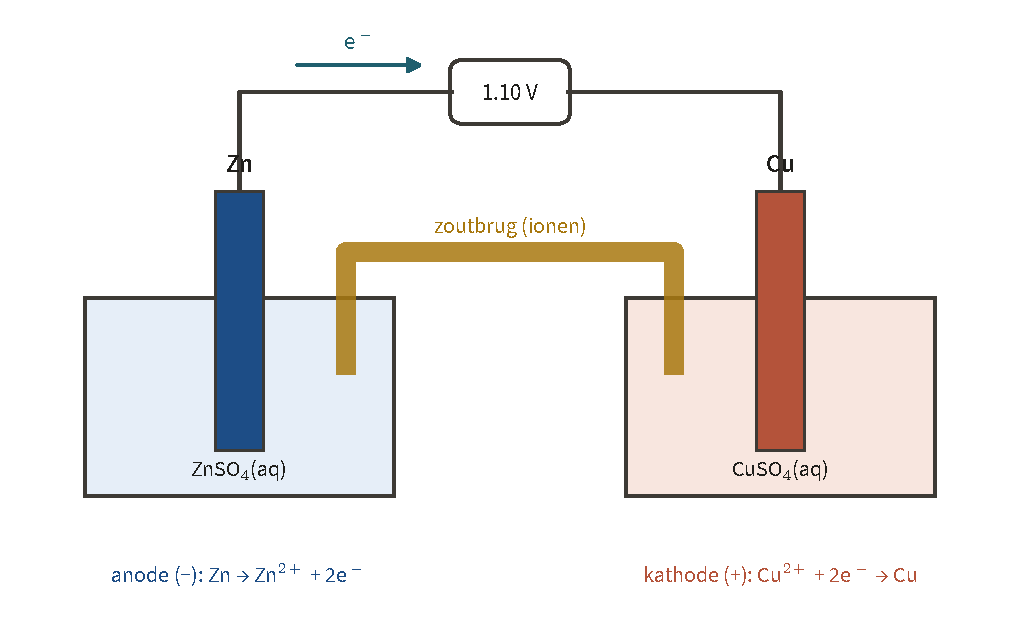
\includegraphics[width=0.8\linewidth]{Figuren/daniell_cel}
    \caption{De Daniell-cel. Zink wordt geoxideerd aan de anode, koperionen worden gereduceerd aan de kathode. Elektronen lopen door de uitwendige draad, ionen door de zoutbrug; samen sluiten ze de stroomkring.}
    \label{fig:daniell-cel}
\end{figure}

\begin{voorbeeld}{De Daniell-cel}
Voor $\mathrm{Zn(s) + Cu^{2+}(aq) \rightarrow Zn^{2+}(aq) + Cu(s)}$ (figuur~\ref{fig:daniell-cel}) is $\Delta_r G^\circ = \SI{-212.3}{\kilo\joule\per\mole}$ en $n = 2$:
\[
E^\circ = -\frac{\Delta_r G^\circ}{nF} = \frac{212\,300}{2 \times 96485} = \SI{1.10}{\volt}.
\]
\end{voorbeeld}

\subsection{De standaardcelpotentiaal en standaardreductiepotentiaal}
\label{sec:standaardreductiepotentiaal}

Een enkele elektrodepotentiaal kan je niet meten, alleen een verschil. Daarom drukt men elke halfreactie uit als \emph{reductiepotentiaal} ten opzichte van de \emph{standaardwaterstofelektrode} (SHE: Pt in $a_{\mathrm{H^+}} = 1$ onder \SI{1}{\bar} \ce{H2}), die per definitie \SI{0}{\volt} is. De celpotentiaal is dan
\begin{equation}
\boxed{\;E^\circ_{\text{cel}} = E^\circ_{\text{kathode}} - E^\circ_{\text{anode}}\;}
\label{eq:Ecel}
\end{equation}
Voor de Daniell-cel: $0.34 - (-0.76) = \SI{1.10}{\volt}$, dezelfde waarde als uit $\Delta_rG^\circ$. Hoe hoger in tabel~\ref{tab:reductiepotentialen}, hoe sterker de oxidator; hoe lager, hoe sterker de reductor.

\begin{table}[htb]
\centering
\small
\begin{tabular}{lc@{\qquad}lc}
\toprule
Halfreactie & $E^\circ$ (V) & Halfreactie & $E^\circ$ (V) \\
\midrule
$\mathrm{F_2 + 2\,e^- \rightarrow 2\,F^-}$ & $+2.87$ & $\mathrm{Cu^{2+} + 2\,e^- \rightarrow Cu}$ & $+0.34$ \\
$\mathrm{Au^+ + e^- \rightarrow Au}$ & $+1.69$ & $\mathrm{2\,H^+ + 2\,e^- \rightarrow H_2}$ & $0.00$ \\
$\mathrm{Cl_2 + 2\,e^- \rightarrow 2\,Cl^-}$ & $+1.36$ & $\mathrm{Fe^{2+} + 2\,e^- \rightarrow Fe}$ & $-0.44$ \\
$\mathrm{O_2 + 4\,H^+ + 4\,e^- \rightarrow 2\,H_2O}$ & $+1.23$ & $\mathrm{Zn^{2+} + 2\,e^- \rightarrow Zn}$ & $-0.76$ \\
$\mathrm{Ag^+ + e^- \rightarrow Ag}$ & $+0.80$ & $\mathrm{Al^{3+} + 3\,e^- \rightarrow Al}$ & $-1.66$ \\
$\mathrm{Fe^{3+} + e^- \rightarrow Fe^{2+}}$ & $+0.77$ & $\mathrm{Na^+ + e^- \rightarrow Na}$ & $-2.71$ \\
 & & $\mathrm{Li^+ + e^- \rightarrow Li}$ & $-3.04$ \\
\bottomrule
\end{tabular}
\caption{Standaardreductiepotentialen bij \SI{298}{\kelvin} (bron: CRC Handbook of Chemistry and Physics).}
\label{tab:reductiepotentialen}
\end{table}

\begin{voorbeeld}{Koper in een zilveroplossing}
Met $E^\circ(\mathrm{Ag^+/Ag}) = \SI{0.80}{\volt}$ als kathode en $E^\circ(\mathrm{Cu^{2+}/Cu}) = \SI{0.34}{\volt}$ als anode is $E^\circ_\text{cel} = \SI{0.46}{\volt}$: $\mathrm{Cu + 2\,Ag^+ \rightarrow Cu^{2+} + 2\,Ag}$ is spontaan. Een koperdraad in zilvernitraat wordt inderdaad met zilverkristallen bedekt.
\end{voorbeeld}

\subsection{De vergelijking van Nernst}
\label{sec:nernst-elektrochemie}

Buiten de standaardtoestand volgt de celpotentiaal uit $\Delta_r G = \Delta_r G^\circ + RT \ln Q$ (hoofdstuk~\ref{ch:reagerend}), gedeeld door $-nF$:
\begin{equation}
\boxed{\;E = E^\circ - \frac{RT}{nF} \ln Q\;}
\label{eq:nernst}
\end{equation}
Bij \SI{298}{\kelvin}, met $\log_{10}$:
\begin{equation}
E = E^\circ - \frac{0.0592}{n} \log_{10} Q.
\label{eq:nernst-log10}
\end{equation}
Een factor tien in $Q$ verschuift de spanning dus met $59/n$ millivolt. Diezelfde \SI{0.0592}{\volt} wordt verderop de helling van de lijnen in een Pourbaix-diagram (\S~\ref{sec:pourbaix-waterlijnen}).

\begin{voorbeeld}{Concentratiecel}
Twee koperelektroden in \SI{0.10}{} en \SI{1.0}{\mole\per\litre} $\mathrm{Cu^{2+}}$: $E^\circ = 0$, maar $E = -\frac{0.0592}{2}\log_{10}(0.10/1.0) = \SI{0.030}{\volt}$. Een concentratieverschil alleen levert al spanning. Zo ontstaat ook corrosie onder een druppel of in een spleet, waar de zuurstofconcentratie lager is.
\end{voorbeeld}

\subsection{De evenwichtsconstante uit de standaardcelpotentiaal}
\label{sec:evenwichtsconstante-elektrochemie}

In evenwicht is $E = 0$ en $Q = K$:
\begin{equation}
\boxed{\;E^\circ = \frac{RT}{nF} \ln K \;\;\Leftrightarrow\;\; \Delta_r G^\circ = -nFE^\circ = -RT \ln K\;}
\label{eq:K-uit-E0}
\end{equation}
Voor $\mathrm{Cu + 2\,Ag^+}$ ($E^\circ = \SI{0.46}{\volt}$, $n = 2$) is $\ln K = 2 \times 96485 \times 0.46/(8.314 \times 298) = 35.8$, dus $K \approx 4\times10^{15}$: de reactie loopt volledig af. Een spanning van enkele tienden volt betekent al een enorme $K$.

\subsubsection{Temperatuursafhankelijkheid van de celpotentiaal: $\Delta_rS^\circ$ en $\Delta_rH^\circ$ zonder calorimetrie}
\label{sec:temperatuur-E}

Leid $\Delta_rG^\circ = -nFE^\circ$ af naar $T$ en gebruik $(\partial \Delta_rG^\circ/\partial T)_p = -\Delta_rS^\circ$:
\begin{gather}
\boxed{\;\Delta_rS^\circ = nF\left(\frac{\partial E^\circ}{\partial T}\right)_p\;}
\label{eq:dSdE}\\
\Delta_rH^\circ = \Delta_rG^\circ + T\Delta_rS^\circ = -nFE^\circ + nFT\left(\frac{\partial E^\circ}{\partial T}\right)_p
\label{eq:dH-uit-E}
\end{gather}
Een spanningsmeting bij enkele temperaturen geeft dus $\Delta_rG^\circ$, $\Delta_rS^\circ$ \'en $\Delta_rH^\circ$, zonder calorimeter. Voor de Daniell-cel is $\partial E^\circ/\partial T \approx \SI{-1.1e-4}{\volt\per\kelvin}$, zodat $\Delta_rS^\circ = 2 \times 96485 \times (-1.1\times10^{-4}) \approx \SI{-21}{\joule\per\mole\per\kelvin}$ en $\Delta_rH^\circ = -212.3 + 298 \times (-0.021) \approx \SI{-218.5}{\kilo\joule\per\mole}$, in overeenstemming met de vormingsenthalpie\"en.

\section{Elektrolyse en de thermodynamische minimumspanning}

Een niet-spontane reactie ($\Delta_r G > 0$) kan je afdwingen met een uitwendige spanning van minstens $\Delta_r G/nF$. In de praktijk is meer nodig, door overspanning aan de elektroden en weerstand in elektrolyt en membraan (\S~\ref{sec:elektrodekinetiek}).

\begin{voorbeeld}{Elektrolyse van water}
Voor $\mathrm{2\,H_2O(l) \rightarrow 2\,H_2(g) + O_2(g)}$ is $\Delta_r G^\circ = \SI{+474.4}{\kilo\joule\per\mole}$ en $n = 4$:
\[
E^\circ_{\text{min}} = \frac{474\,400}{4 \times 96485} = \SI{1.23}{\volt}.
\]
Industri\"ele elektrolysers werken bij \SIrange{1.7}{2.2}{\volt}, vooral door de overspanning aan de zuurstofelektrode.
\end{voorbeeld}

\paragraph{Omkeerbare en thermoneutrale spanning.} De \SI{1.23}{\volt} dekt enkel $\Delta_rG^\circ$. De reactie vraagt in totaal $\Delta_rH^\circ = \SI{571.6}{\kilo\joule}$; het verschil $T\Delta_rS^\circ$ moet als warmte binnenkomen. Levert de stroom ook die warmte, dan is $U_\mathrm{tn} = \Delta_rH^\circ/nF = \SI{1.48}{\volt}$, de \emph{thermoneutrale spanning}. Figuur~\ref{fig:waterstof-spanning} vertaalt elke spanning met Faraday naar elektriciteit per kilogram waterstof.

\begin{figure}[htb]
    \centering
    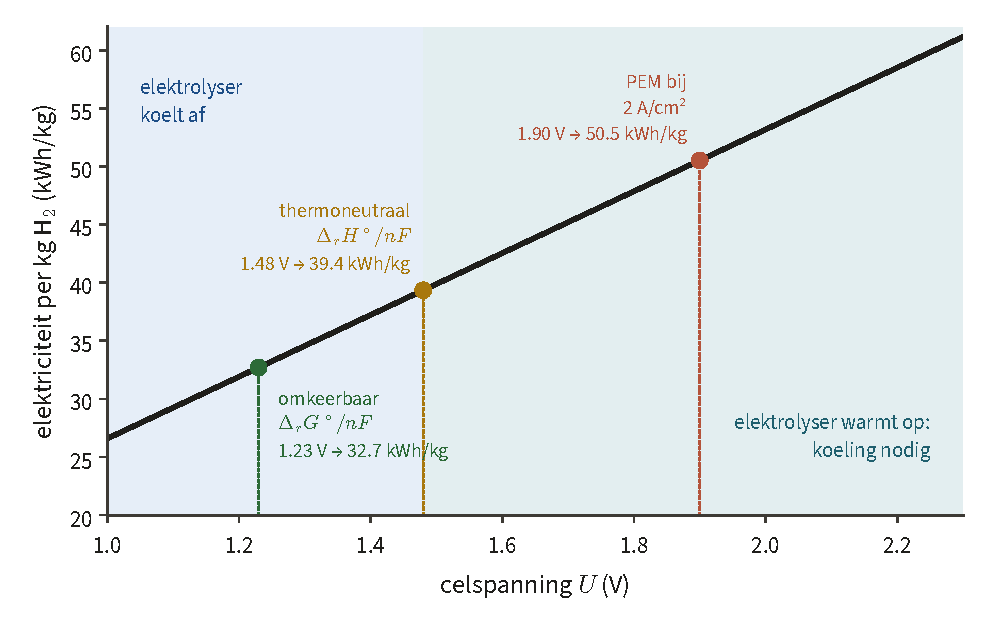
\includegraphics[width=0.72\linewidth]{Figuren/waterstof_spanning}
    \caption{Elektriciteitsverbruik per kilogram waterstof in functie van de celspanning (vergelijking~\eqref{eq:energie-per-kg} met $n = 2$, $\eta_F = 1$). Bij \SI{1.48}{\volt} is het verbruik gelijk aan de verbrandingswarmte (HHV) van waterstof. Daaronder koelt de elektrolyser af, daarboven moet hij gekoeld worden.}
    \label{fig:waterstof-spanning}
\end{figure}

\subsection{De galvanische cel en de batterij}

In een galvanische cel zijn oxidatie (aan de \emph{anode}) en reductie (aan de \emph{kathode}) ruimtelijk gescheiden, zodat de elektronen door een uitwendige kring moeten. Een \emph{batterij} is zo'n cel, gebouwd om energie op te slaan. Primaire batterijen (alkalisch Zn--\ce{MnO2}) ontlaad je \'e\'en keer; secundaire (lood, lithium-ion) laad je op door elektrolyse in de omgekeerde richting.

\begin{voorbeeld}{Hoeveel energie past er in een kilogram batterij?}
De loodaccu werkt met $\mathrm{Pb + PbO_2 + 2\,H_2SO_4 \rightleftharpoons 2\,PbSO_4 + 2\,H_2O}$, $E^\circ = \SI{2.04}{\volt}$ (zes cellen geven \SI{12}{\volt}). Het vaste \ce{PbSO4} blijft op de elektroden zitten, daarom is hij herlaadbaar. Met $n = 2$ en \SI{642.6}{\gram} reagentia:
\[
\frac{2 \times 96485 \times 2.04}{0.6426} = \SI{6.1e5}{\joule\per\kilogram} = \SI{170}{\watt\hour\per\kilogram}.
\]
Voor lithium-ion ($\mathrm{LiC_6 + CoO_2 \rightarrow C_6 + LiCoO_2}$, $n = 1$, \SI{3.7}{\volt}, \SI{169.9}{\gram}) is dat \SI{580}{\watt\hour\per\kilogram}. Echte cellen halen een kwart (lood: \SIrange{30}{40}{\watt\hour\per\kilogram}) tot de helft (Li-ion: \SIrange{150}{270}{\watt\hour\per\kilogram}) van de theorie. Hoge spanning en lichte elementen maakten de elektrische auto mogelijk.
\end{voorbeeld}

\subsection{Brandstofcellen}

Een \emph{brandstofcel} zet continu toegevoerde brandstof (meestal \ce{H2}) en zuurstof om in stroom: de omgekeerde waterelektrolyse, met $E^\circ = \SI{1.23}{\volt}$. Een PEM-cel levert in de praktijk \SIrange{0.6}{0.8}{\volt}, door dezelfde kinetische verliezen.

\section{Elektrodekinetiek in het kort: waarom de spanning afwijkt}
\label{sec:elektrodekinetiek}

Thermodynamica geeft de spanning bij stroom nul. Met stroom verliest een galvanische cel spanning en vraagt een elektrolyser er extra. Dat verschil met de evenwichtspotentiaal heet \emph{overspanning} $\eta$, met drie bronnen:
\begin{itemize}
\item \textbf{activering}: elektronenoverdracht heeft een activeringsenergie (hoofdstuk~\ref{ch:kinetiek});
\item \textbf{ohmse verliezen}: elektrolyt, membraan en contacten hebben weerstand, verlies $iR$;
\item \textbf{concentratie}: bij hoge stroom raken de reagentia aan het oppervlak op; diffusie begrenst de stroom.
\end{itemize}
Voor de activeringsoverspanning geldt bij voldoende stroom de \emph{vergelijking van Tafel}:
\begin{equation}
\boxed{\;\eta = b\,\log_{10}\frac{i}{i_0}\;}
\label{eq:tafel}
\end{equation}
met $i$ de stroomdichtheid, $b$ de \emph{Tafelhelling} (\SIrange{0.03}{0.12}{\volt} per decade) en $i_0$ de \emph{uitwisselingsstroomdichtheid}: hoe snel de reactie in evenwicht heen en terug gaat. Die hangt sterk af van het elektrodemateriaal: voor waterstofontwikkeling \SI{e-3}{\ampere\per\centi\metre\squared} op platina, \SI{e-12}{} op kwik. Een elektrokatalysator verhoogt $i_0$ zonder de evenwichtspotentiaal te veranderen, zoals elke katalysator.

\begin{figure}[htb]
    \centering
    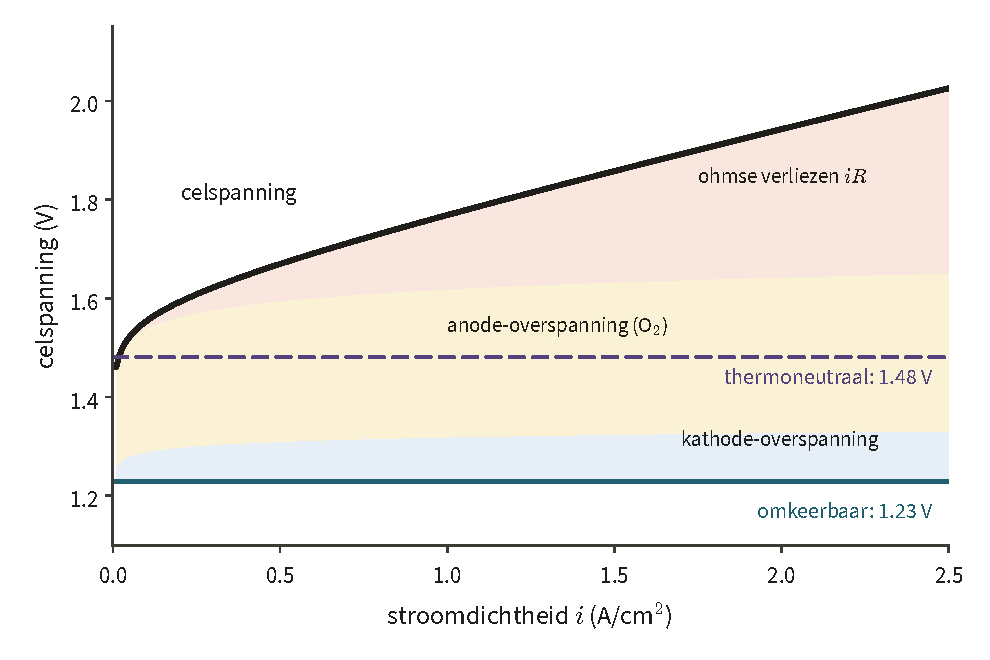
\includegraphics[width=0.75\linewidth]{Figuren/elektrolyser_polarisatie}
    \caption{Celspanning van een PEM-elektrolyser als functie van de stroomdichtheid, opgesplitst in de omkeerbare spanning en de drie verliezen (illustratieve parameters). De zuurstofelektrode is de grootste kinetische rem; bij hoge stroom wegen de ohmse verliezen door.}
    \label{fig:elektrolyser-polarisatie}
\end{figure}

\begin{toepassing}{Rendement van elektrolysers en brandstofcellen}
Een PEM-elektrolyser bij \SI{2}{\ampere\per\centi\metre\squared} werkt rond \SI{1.9}{\volt} (figuur~\ref{fig:elektrolyser-polarisatie}): een rendement van $1.48/1.9 = \SI{78}{\percent}$ (HHV). Een brandstofcel bij \SI{0.7}{\volt} haalt $0.7/1.48 = \SI{47}{\percent}$. De keten stroom $\rightarrow$ waterstof $\rightarrow$ stroom verliest dus meer dan de helft. De ontwerper kiest telkens tussen een grote stroomdichtheid (kleine, goedkope stack) en een lage spanning (hoog rendement).
\end{toepassing}

Corrosie is ook een elektrodeproces, en daar komt dezelfde kinetiek terug (\S~\ref{sec:corrosiesnelheid}).

\section{Corrosie en het Pourbaix-diagram}

\subsection{Corrosie als spontane galvanische cel}
\label{sec:corrosie-galvanisch}
\label{sec:corrosie}

Corrosie is een galvanische cel die niemand wil: het metaal is de anode en wordt geoxideerd, terwijl zuurstof of H$^+$ wordt gereduceerd. Voor ijzer in belucht water:
\begin{align}
\mathrm{Fe} &\rightarrow \mathrm{Fe^{2+}} + 2\,e^-, & E^\circ&=\SI{-0.44}{\volt}\ \text{(reductiepotentiaal, tabel~\ref{tab:reductiepotentialen})},\\
\mathrm{O_2 + 4\,H^+ + 4\,e^-} &\rightarrow \mathrm{2\,H_2O}, & E^\circ&=\SI{1.23}{\volt}.
\end{align}

\begin{voorbeeld}{De drijvende kracht achter roestvorming}
De volledige corrosiereactie is $\mathrm{2\,Fe + O_2 + 4\,H^+ \rightarrow 2\,Fe^{2+} + 2\,H_2O}$, met $n=4$. De standaardcelpotentiaal bedraagt
\[
E^\circ_{\text{cel}} = E^\circ_{\text{kathode}} - E^\circ_{\text{anode}} = \SI{1.23}{\volt} - (\SI{-0.44}{\volt}) = \SI{1.67}{\volt}.
\]
We passen de Nernstvergelijking~\eqref{eq:nernst} toe op typische omstandigheden: neutraal water (pH~7, dus $a_{\mathrm{H^+}}=10^{-7}$), lucht ($p_{\mathrm{O_2}}\approx\SI{0.21}{\bar}$) en een spoor opgelost $\mathrm{Fe^{2+}}$ ($a_{\mathrm{Fe^{2+}}}\approx10^{-6}$):
\[
Q = \frac{a_{\mathrm{Fe^{2+}}}^2}{p_{\mathrm{O_2}}\cdot a_{\mathrm{H^+}}^4} = \frac{(10^{-6})^2}{(0.21)(10^{-7})^4} \approx 4.8\times10^{16}.
\]
\[
E = E^\circ_{\text{cel}} - \frac{RT}{nF}\ln Q = \SI{1.67}{\volt} - \frac{(\SI{8.314}{})( \SI{298}{})}{(4)(\SI{96485}{})}\ln(4.8\times10^{16}) \approx \SI{1.42}{\volt}.
\]
Ook onder realistische omstandigheden blijft $E$ sterk positief ($\Delta_rG \approx \SI{-549}{\kilo\joule\per\mole}$). De thermodynamica biedt geen enkele rem: bescherming (verf, coatings, legeren, kathodische bescherming, \S~\ref{sec:sturen-stabiliteit}) is onmisbaar.
\end{voorbeeld}

\subsection{Hoe snel corrodeert een metaal?}
\label{sec:corrosiesnelheid}

De thermodynamica zegt \emph{of} een metaal corrodeert; de ingenieur wil weten \emph{hoeveel millimeter per jaar}. Omdat corrosie een elektrochemische reactie is, volgt de snelheid rechtstreeks uit de \emph{corrosiestroomdichtheid} $i_\mathrm{corr}$ en de wet van Faraday (vergelijking~\eqref{eq:faraday}). Delen door de dichtheid $\rho$ geeft de dikte die per tijdseenheid verdwijnt:
\begin{equation}
\boxed{\;v_\mathrm{corr} = \frac{i_\mathrm{corr}\,M}{nF\rho}\;}
\label{eq:corrosiesnelheid}
\end{equation}

\begin{voorbeeld}{Van microampère naar millimeter per jaar}
Voor staal ($M = \SI{55.85}{\gram\per\mole}$, $n=2$, $\rho = \SI{7.87}{\gram\per\centi\metre\cubed}$) en $i_\mathrm{corr} = \SI{1}{\micro\ampere\per\centi\metre\squared}$:
\[
v_\mathrm{corr} = \frac{(\SI{e-6}{\ampere\per\centi\metre\squared})(\SI{55.85}{\gram\per\mole})}{(2)(\SI{96485}{\coulomb\per\mole})(\SI{7.87}{\gram\per\centi\metre\cubed})} = \SI{3.7e-11}{\centi\metre\per\second} = \SI{0.012}{\milli\metre}/jaar.
\]
Een handige vuistregel: \SI{1}{\micro\ampere\per\centi\metre\squared} komt voor staal overeen met ongeveer \SI{12}{\micro\metre} per jaar. Onbeschermd staal in zeewater corrodeert met \SIrange{0.1}{0.2}{\milli\metre}/jaar, dus \SIrange{10}{20}{\micro\ampere\per\centi\metre\squared}. Daarom voorziet de ontwerper van een drukvat of leiding een \emph{corrosietoeslag}: typisch \SI{3}{\milli\metre} extra wanddikte voor twintig jaar dienst.
\end{voorbeeld}

Waar komt $i_\mathrm{corr}$ vandaan? Op een corroderend metaal lopen twee reacties tegelijk: de oxidatie van het metaal (anodisch) en de reductie van zuurstof of H$^+$ (kathodisch). Er loopt geen netto stroom naar buiten, dus beide stromen zijn even groot. Het metaal neemt vanzelf de potentiaal aan waar dat zo is: de \emph{corrosiepotentiaal} $E_\mathrm{corr}$. Een \emph{Evansdiagram} (figuur~\ref{fig:evans}) zet beide Tafellijnen uit tegen de logaritme van de stroom; hun snijpunt geeft $E_\mathrm{corr}$ en $i_\mathrm{corr}$.

\begin{figure}[htb]
    \centering
    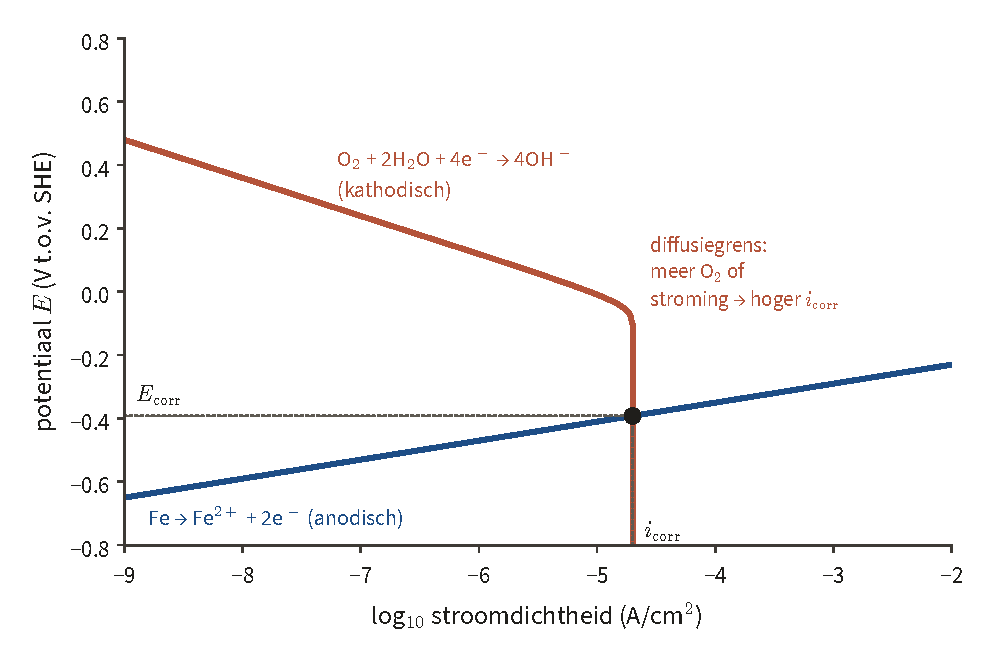
\includegraphics[width=0.75\linewidth]{Figuren/evans_diagram}
    \caption{Evansdiagram van staal in belucht water (schematisch). Het snijpunt van de anodische en de kathodische lijn bepaalt de corrosiepotentiaal en de corrosiestroom. Hier wordt de kathodische stroom begrensd door de aanvoer van zuurstof.}
    \label{fig:evans}
\end{figure}

Het Evansdiagram verklaart enkele vaststellingen uit de praktijk:
\begin{itemize}
\item In neutraal water is de aanvoer van opgeloste zuurstof meestal de traagste stap. Meer zuurstof, hogere temperatuur of sterkere stroming verschuift de diffusiegrens naar rechts en verhoogt $i_\mathrm{corr}$. Ontgassen van ketelvoedingswater (hoofdstuk~\ref{ch:niet-reagerend}) haalt precies die kathodische reactie weg.
\item Twee verschillende metalen in contact vormen een \emph{galvanisch koppel}: het minst edele metaal wordt anode. De verhouding van de oppervlakken telt: een kleine anode tegenover een grote kathode concentreert de volledige kathodische stroom op een klein stuk metaal. Stalen klinknagels in een koperen plaat zijn dus een slecht idee, koperen klinknagels in een stalen plaat veel minder.
\item Een opofferingsanode (zink, magnesium) of een uitwendige stroombron verschuift de potentiaal van het staal naar beneden, tot onder de evenwichtspotentiaal van ijzer: de anodische stroom van het staal valt weg (\S~\ref{sec:sturen-stabiliteit}).
\end{itemize}

\subsection{Het Pourbaix-diagram}
\label{sec:pourbaix}

Het \emph{Pourbaix-diagram} is het fasediagram van de elektrochemie. Waar een gewoon fasediagram (\S~\ref{sec:fasediagram}) de stabiele fase toont in functie van $T$ en $p$, toont een Pourbaix-diagram de stabiele vorm van een element in functie van de potentiaal $E$ (de oxiderende kracht van de omgeving) en de pH (want veel reacties verbruiken H$^+$ of OH$^-$). Het verdeelt het vlak in drie soorten gebieden:
\begin{itemize}
\item \textbf{immuniteit}: het metaal zelf is stabiel;
\item \textbf{corrosie}: opgeloste ionen zijn stabieler, het metaal lost op;
\item \textbf{passiviteit}: een vast oxide of hydroxide is stabiel en kan het metaal afschermen.
\end{itemize}
Op elke grenslijn hebben de twee soorten dezelfde Gibbs-energie. Reacties met enkel elektronen geven horizontale lijnen, reacties met enkel H$^+$ verticale, en reacties met beide schuine lijnen, waarvan Nernst de helling geeft.

\subsubsection{Het stabiliteitsgebied van water: afleiding van de grenslijnen}
\label{sec:pourbaix-waterlijnen}

Vrijwel alle Pourbaix-diagrammen bevatten twee schuine lijnen die het stabiliteitsgebied van water begrenzen. Buiten deze grenzen is vloeibaar water thermodynamisch niet stabiel. We leiden beide lijnen expliciet af met de vergelijking van Nernst (vergelijking~\eqref{eq:nernst}).

\textbf{Bovengrens: oxidatie van water tot zuurstof.} Bij hoge potentiaal wordt water geoxideerd:
\[
\mathrm{2\,H_2O \rightleftharpoons O_2 + 4\,H^+ + 4\,e^-}, \qquad E^\circ=\SI{1.23}{\volt}\ (n=4).
\]
Met $a_{\mathrm{H_2O}}\approx1$ en, als referentie, $p_{\mathrm{O_2}}=\SI{1}{\bar}$, is het reactiequoti\"ent voor de \emph{reductie}-vorm $Q=1/a_{\mathrm{H^+}}^4$. De Nernstvergelijking geeft:
\[
E = E^\circ - \frac{RT}{4F}\ln\frac{1}{a_{\mathrm{H^+}}^4} = E^\circ + \frac{RT}{F}\ln a_{\mathrm{H^+}}.
\]
Met $\ln a_{\mathrm{H^+}} = -\ln(10)\cdot\mathrm{pH}$ en $RT\ln(10)/F=\SI{0.0592}{\volt}$ bij \SI{298}{\kelvin} (\S~\ref{sec:nernst-elektrochemie}):
\begin{equation}
\boxed{\;E_{\mathrm{O_2/H_2O}} = \SI{1.23}{\volt} - \num{0.0592}\cdot\mathrm{pH}.\;}
\label{eq:lijn-boven}
\end{equation}

\textbf{Ondergrens: reductie van water tot waterstof.} Bij lage potentiaal wordt water (via $\mathrm{H^+}$) gereduceerd tot waterstofgas:
\[
\mathrm{2\,H^+ + 2\,e^- \rightleftharpoons H_2}, \qquad E^\circ=\SI{0}{\volt}\ (n=2).
\]
Met $p_{\mathrm{H_2}}=\SI{1}{\bar}$ als referentie is $Q=1/a_{\mathrm{H^+}}^2$, zodat op dezelfde manier:
\begin{equation}
\boxed{\;E_{\mathrm{H^+/H_2}} = 0 - \num{0.0592}\cdot\mathrm{pH}.\;}
\label{eq:lijn-onder}
\end{equation}

Beide lijnen dalen met \SI{0.0592}{\volt} per pH-eenheid en blijven \SI{1.23}{\volt} uit elkaar (figuur~\ref{fig:pourbaix-generiek}). Bij pH~7 ligt de bovengrens op \SI{0.82}{\volt}, de ondergrens op \SI{-0.41}{\volt}. Daartussen is water stabiel; erboven ontwikkelt het zuurstof, eronder waterstof. Bijna alle corrosie in de praktijk speelt zich tussen die twee lijnen af.

\begin{figure}[htb]
    \centering
    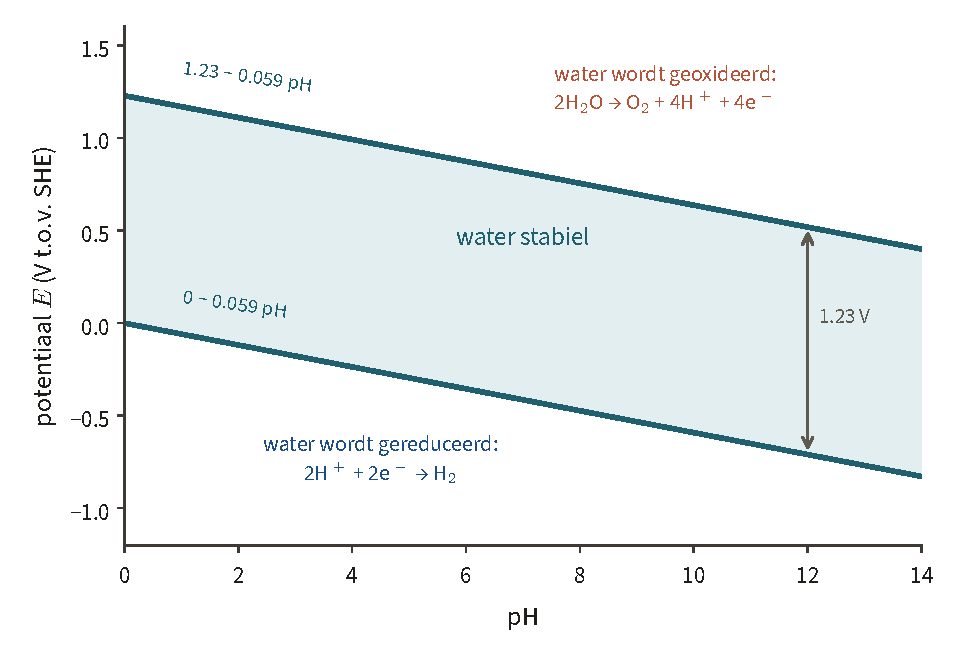
\includegraphics[width=0.75\linewidth]{Figuren/pourbaix_water}
    \caption{Het stabiliteitsgebied van water. Beide grenslijnen dalen met \SI{0.0592}{\volt} per pH-eenheid en liggen altijd \SI{1.23}{\volt} uit elkaar. In de volgende Pourbaix-diagrammen zijn ze als stippellijnen ingetekend.}
    \label{fig:pourbaix-generiek}
\end{figure}

\subsection{Zelf een Pourbaix-diagram opstellen: zink}
\label{sec:pourbaix-zelf}

Een Pourbaix-diagram is geen mysterie: het volgt volledig uit tabelwaarden van $\Delta_fG^\circ$ en de vergelijking van Nernst. We stellen het diagram van zink stap voor stap op.

\paragraph{Stap 1: kies de soorten en zoek $\Delta_fG^\circ$.} We beperken ons tot de vier belangrijkste vormen van zink in water (waarden in kJ/mol bij \SI{298}{\kelvin}, uit de NBS-tabellen):
\begin{center}
\begin{tabular}{lcccc}
\toprule
soort & Zn(s) & Zn$^{2+}$(aq) & Zn(OH)$_2$(s) & ZnO$_2^{2-}$(aq) \\
$\Delta_fG^\circ$ & 0 & $-147.1$ & $-553.5$ & $-384.2$ \\
\bottomrule
\end{tabular}
\end{center}
Daarnaast is $\Delta_fG^\circ(\mathrm{H_2O,l}) = \SI{-237.1}{\kilo\joule\per\mole}$ en $\Delta_fG^\circ(\mathrm{H^+}) = 0$.

\paragraph{Stap 2: kies de activiteit van de opgeloste ionen.} Bij corrosie stelt men de grens meestal bij $a = 10^{-6}$: lost er minder dan dat op, dan noemt men het metaal praktisch niet aangetast.

\paragraph{Stap 3: schrijf elke grensreactie en pas Nernst toe.} Elke grens is een evenwicht tussen twee soorten. Er zijn drie types.

\emph{Horizontale lijn, enkel elektronen.} $\mathrm{Zn^{2+} + 2\,e^- \rightleftharpoons Zn}$ met $E^\circ = \Delta_fG^\circ(\mathrm{Zn^{2+}})/2F = \SI{-0.762}{\volt}$:
\[
E = -0.762 + \frac{0.0592}{2}\log a_{\mathrm{Zn^{2+}}} = -0.762 - 0.178 = \SI{-0.94}{\volt}.
\]

\emph{Verticale lijn, enkel H$^+$.} $\mathrm{Zn(OH)_2 + 2\,H^+ \rightleftharpoons Zn^{2+} + 2\,H_2O}$ heeft $\Delta_rG^\circ = -147.1 + 2(-237.1) - (-553.5) = \SI{-67.8}{\kilo\joule\per\mole}$, dus $\log K = 67\,800/(2.303\,RT) = 11.9$. Met $K = a_{\mathrm{Zn^{2+}}}/a_{\mathrm{H^+}}^2$ volgt $\log a_{\mathrm{Zn^{2+}}} = 11.9 - 2\,\mathrm{pH}$, en de grens $a = 10^{-6}$ ligt bij pH~8.9. Op dezelfde manier ligt de grens Zn(OH)$_2$/ZnO$_2^{2-}$ bij pH~11.8.

\emph{Schuine lijn, elektronen en H$^+$.} $\mathrm{Zn(OH)_2 + 2\,H^+ + 2\,e^- \rightleftharpoons Zn + 2\,H_2O}$ heeft $\Delta_rG^\circ = 2(-237.1) - (-553.5) = \SI{79.2}{\kilo\joule\per\mole}$, dus $E^\circ = -79\,200/2F = \SI{-0.41}{\volt}$ en
\[
E = -0.41 - 0.0592\,\mathrm{pH}.
\]
Per H$^+$ per elektron daalt de lijn met \SI{0.0592}{\volt} per pH-eenheid, net als de waterlijnen.

\paragraph{Stap 4: teken en controleer.} De lijnen snijden elkaar; van elke lijn houd je enkel het stuk waar beide soorten ook echt de stabielste zijn. Figuur~\ref{fig:pourbaix-zink} toont het resultaat. Een rekenblad kan hetzelfde zonder lijnen te zoeken: bereken voor elk punt $(E, \mathrm{pH})$ de Gibbsenergie van elke soort ten opzichte van het metaal en kleur het punt volgens de laagste waarde. Zo zijn alle diagrammen in dit hoofdstuk berekend.

\begin{figure}[htb]
    \centering
    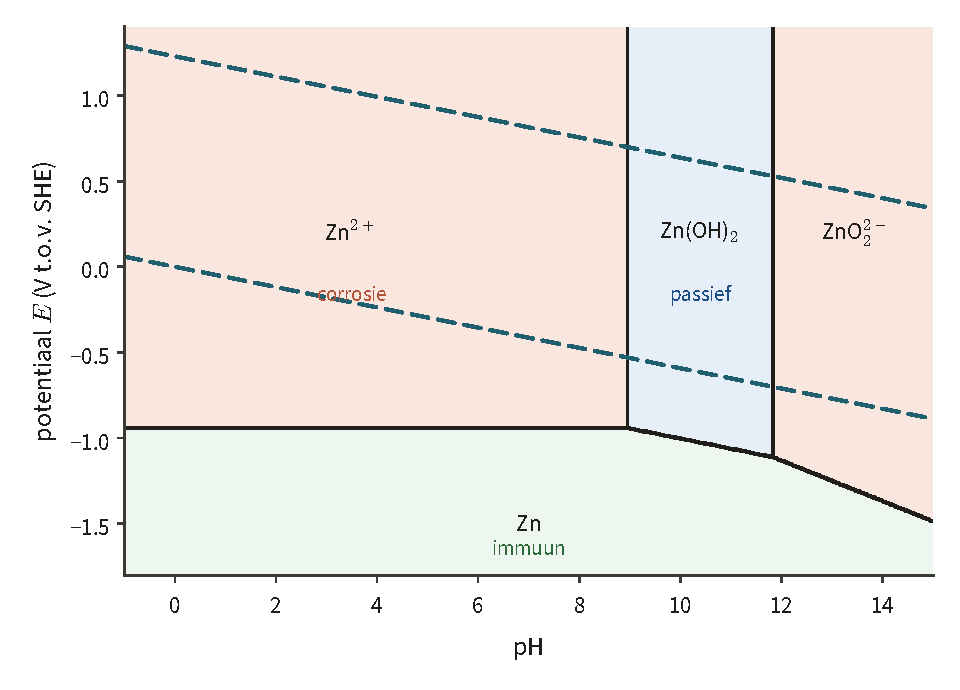
\includegraphics[width=0.75\linewidth]{Figuren/pourbaix_zink}
    \caption{Pourbaix-diagram van zink bij \SI{25}{\celsius} en ionactiviteit $10^{-6}$ (berekend uit NBS-gegevens). Rood: corrosie, blauw: passief, groen: immuun. Stippellijnen: stabiliteitsgebied van water.}
    \label{fig:pourbaix-zink}
\end{figure}

\begin{toepassing}{Waarom verzinkt staal zo goed werkt}
Zink is \emph{amfoteer}: het lost op in zuur (Zn$^{2+}$) en in sterke base (ZnO$_2^{2-}$), maar tussen pH~9 en~12 vormt het een beschermende hydroxide- en carbonaatlaag. In regenwater en de meeste natuurlijke milieus ligt de pH daar niet ver vandaan, zodat een zinklaag maar traag verdwijnt (enkele \si{\micro\metre} per jaar). Raakt de laag beschadigd, dan wordt het blootgestelde staal kathodisch beschermd: zink ligt in het diagram veel lager dan ijzer en offert zich op. Daarom is verzinken (thermisch of galvanisch) de goedkoopste duurzame bescherming voor vangrails, bouwstaal en elektriciteitsmasten. In beton (pH~13) of in contact met kalk werkt zink veel minder goed, wat het diagram ook toont.
\end{toepassing}

\subsection{Het Pourbaix-diagram van ijzer}
\label{sec:pourbaix-ijzer}

Het diagram van ijzer (figuur~\ref{fig:pourbaix-ijzer}) toont:

\begin{itemize}
\item Bij lage potentialen: immuniteit (metaal Fe stabiel), onder ongeveer \SI{-0.6}{\volt}.
\item Bij lage pH: corrosie, als opgelost $\mathrm{Fe^{2+}}$ of, bij hoge potentiaal, $\mathrm{Fe^{3+}}$.
\item Bij neutrale tot basische pH: passiviteit door de vaste oxiden magnetiet ($\mathrm{Fe_3O_4}$) en hematiet ($\mathrm{Fe_2O_3}$).
\end{itemize}
Een belangrijke vaststelling: de immuniteitsgrens van ijzer ligt bij elke pH \emph{onder} de onderste waterlijn. IJzer is dus nergens stabiel in contact met water. In zuur water (lage pH, lage potentiaal) corrodeert het zelfs zonder zuurstof, met H$^+$ als oxidator en waterstofgas als product.

\begin{figure}[htb]
    \centering
    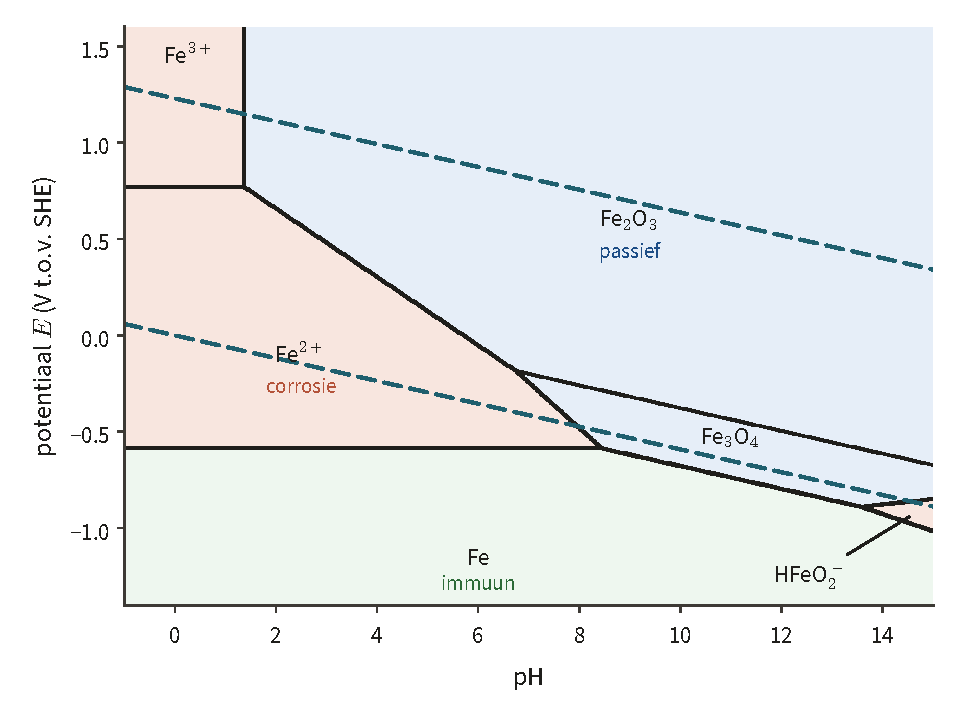
\includegraphics[width=0.75\linewidth]{Figuren/pourbaix_ijzer}
    \caption{Pourbaix-diagram van ijzer bij \SI{25}{\celsius} en ionactiviteit $10^{-6}$ (berekend uit NBS-gegevens; Fe(OH)$_2$ en FeOOH zijn weggelaten). Bij neutrale pH en beluchting (bovenaan het watergebied) ligt ijzer in het gebied van Fe$_2$O$_3$; zonder lucht (onderaan) in dat van Fe$^{2+}$ of Fe$_3$O$_4$.}
    \label{fig:pourbaix-ijzer}
\end{figure}

Het diagram voorspelt dat ijzer in belucht neutraal water passief zou zijn. Toch roest een stalen balk. IJzeroxiden zijn echter poreus en weinig hechtend, zodat de bescherming onvolledig is; bovendien verschuiven chloride-ionen de grenzen in het nadeel van de passieve laag. Daarom wordt staal gecoat, geverfd of gelegeerd met chroom (roestvast staal), dat een veel compactere oxidefilm vormt.

\section{Materiaalkeuze en corrosiebeheersing}

\subsection{Materiaalkeuze op basis van Pourbaix-diagrammen}
\label{sec:materiaalkeuze}

Een Pourbaix-diagram zegt welke toestand stabiel is, niet hoe snel die bereikt wordt. Een metaal in het corrosiegebied kan praktisch onaangetast blijven als de reactie traag is; een metaal in het passieve gebied kan toch corroderen als de oxidefilm lokaal beschadigd raakt. Materiaalkeuze combineert dus altijd thermodynamica en kinetiek.

\begin{voorbeeld}{Aluminium: thermodynamisch reactief, praktisch inert}
Aluminium bezit een sterk negatieve standaardpotentiaal ($E^\circ = \SI{-1.66}{\volt}$, tabel~\ref{tab:reductiepotentialen}), wat erop wijst dat oxidatie thermodynamisch zeer gunstig is. Toch behoort aluminium tot de meest corrosiebestendige constructiematerialen. De verklaring ligt in de vorming van een uiterst dunne, compacte en sterk hechtende laag aluminiumoxide, die het onderliggende metaal afschermt van de omgeving. Figuur~\ref{fig:pourbaix-al-cu} toont dat aluminium enkel passief is tussen pH~4.5 en~9. Daarbuiten lost het oxide op: in zuur als Al$^{3+}$, in base als aluminaat Al(OH)$_4^-$. Daarom mag een aluminium pan niet in de vaatwasmachine met een sterk alkalisch vaatwasmiddel, en ontkalkt men aluminium niet met sterk zuur.
\end{voorbeeld}

\begin{figure}[htb]
    \centering
    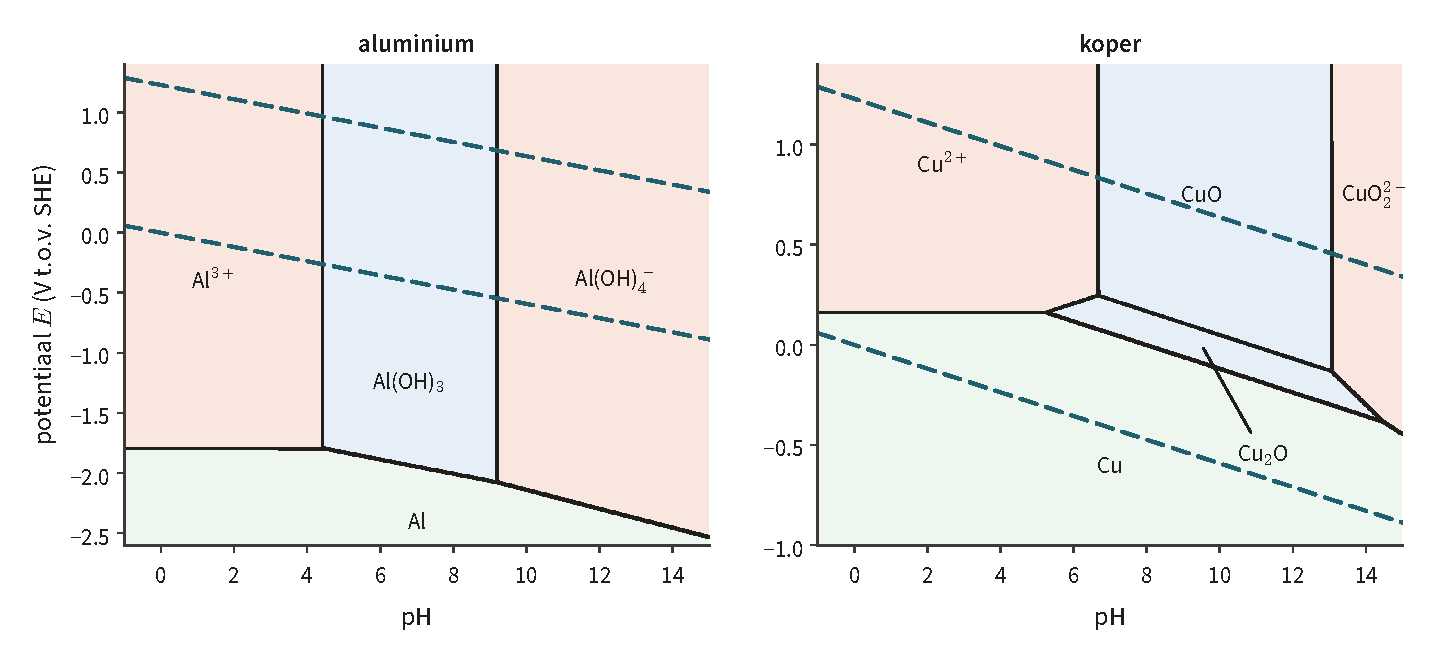
\includegraphics[width=\linewidth]{Figuren/pourbaix_al_cu}
    \caption{Pourbaix-diagrammen van aluminium (links) en koper (rechts) bij \SI{25}{\celsius} en ionactiviteit $10^{-6}$ (berekend uit NBS-gegevens). Let op de verschillende schaal van de potentiaalas.}
    \label{fig:pourbaix-al-cu}
\end{figure}

\begin{voorbeeld}{Koper: een edel metaal in zuur zonder lucht}
Bij koper ligt het immuniteitsgebied grotendeels \emph{boven} de onderste waterlijn (figuur~\ref{fig:pourbaix-al-cu}). In zuur water zonder opgeloste zuurstof is H$^+$ dus niet sterk genoeg om koper te oxideren: koper lost niet op in verdund zoutzuur, zink en ijzer wel. Met lucht erbij verschuift de potentiaal naar boven en komt koper in het Cu$^{2+}$-gebied terecht; daarom corrodeert koper wel in belucht zuur. Bij neutrale pH vormt koper een laagje Cu$_2$O en, buiten, op termijn het groene patina. Koperen waterleidingen gaan zo decennia mee, tenzij het water zuur en zuurstofrijk is.
\end{voorbeeld}

\begin{voorbeeld}{Roestvast staal}
Roestvast staal bevat minstens \SI{12}{\percent} chroom. Chroom vormt een compacte oxidefilm ($\mathrm{Cr_2O_3}$) die het onderliggende staal afschermt. Volgens het Pourbaix-diagram bevindt chroom zich in een groot passiviteitsgebied, terwijl de kinetiek van de oxidevorming uiterst gunstig is. De combinatie van beide eigenschappen leidt tot de uitstekende corrosieweerstand die roestvast staal kenmerkt.
\end{voorbeeld}

\subsection{Het sturen van thermodynamische stabiliteit}
\label{sec:sturen-stabiliteit}

Door de procesomstandigheden te wijzigen kan de ingenieur het werkpunt in het Pourbaix-diagram doelgericht verschuiven.

\begin{itemize}
\item \textbf{pH-wijziging}: toevoegen van zuur of base verschuift het punt horizontaal. Voor vele metalen leidt een verhoging van de pH tot passiviteit.
\item \textbf{Potentiaalwijziging}: een uitwendige spanning (kathodische bescherming) verschuift het punt verticaal naar het immuniteitsgebied.
\item \textbf{Legeren}: toevoegen van chroom, nikkel of molybdeen verandert het Pourbaix-diagram zelf.
\item \textbf{Inhibitors}: stoffen die de oxidefilm versterken of de corrosiekinetiek vertragen.
\end{itemize}

\begin{toepassing}{Kathodische bescherming van ondergrondse leidingen}
Aardgasleidingen en opslagtanks worden vaak kathodisch beschermd door een kleine gelijkstroom aan te leggen tussen het te beschermen staal en een ``opofferingsanode'' (magnesium of zink). Hierdoor wordt het staal tot een potentiaal gedwongen waar het zich in het immuniteitsgebied van zijn Pourbaix-diagram bevindt. De anode corrodeert langzaam en moet periodiek worden vervangen, maar de dure leiding blijft gespaard.
\end{toepassing}

\section{Samenvatting en reflectie}

Batterijen, brandstofcellen, elektrolysers en corrosie lijken verschillende werelden, maar ze steunen op dezelfde thermodynamica: $\Delta_rG = -nFE$ verbindt de spanning met de Gibbsenergie van hoofdstuk~\ref{ch:spontaniteit} en het evenwicht van hoofdstuk~\ref{ch:reagerend}. Of je nu groene waterstof produceert, een batterij kiest of een leiding beschermt, je stelt telkens dezelfde vragen: welke spanning laat de thermodynamica toe, hoeveel lading is nodig (Faraday), en hoeveel gaat verloren aan kinetiek? In het volgende hoofdstuk kijken we naar wat er aan oppervlakken gebeurt, waar ook de elektrodereacties plaatsvinden.

\begin{samenvatting}{Elektrochemische thermodynamica}
\begin{itemize}
\item De maximale niet-expansiearbeid is $-\Delta G$; in een cel wordt die elektrische arbeid: $\Delta_rG = -nFE$ en $\Delta_rG^\circ = -nFE^\circ = -RT\ln K$.
\item $E^\circ_\mathrm{cel} = E^\circ_\mathrm{kathode} - E^\circ_\mathrm{anode}$, met reductiepotentialen ten opzichte van de SHE.
\item Nernst: $E = E^\circ - (RT/nF)\ln Q$; bij \SI{298}{\kelvin} \SI{0.0592}{\volt}/$n$ per decade.
\item $(\partial E^\circ/\partial T)_p$ geeft $\Delta_rS^\circ$, en daarmee $\Delta_rH^\circ$, zonder calorimetrie.
\item Faraday: $m = ItM/nF$; energie per kg product $nFU/(M\eta_F)$. Water splitsen vraagt minstens \SI{1.23}{\volt} (omkeerbaar) en \SI{1.48}{\volt} zonder warmtetoevoer (thermoneutraal).
\item Overspanning (activering, ohmse verliezen, diffusie) maakt een elektrolyser duurder en een batterij zwakker. Tafel: $\eta = b\log(i/i_0)$; een katalysator verhoogt $i_0$.
\item Corrosie is een galvanische cel op \'e\'en metaal. De snelheid volgt uit $i_\mathrm{corr}$ via Faraday: \SI{1}{\micro\ampere\per\centi\metre\squared} $\approx$ \SI{12}{\micro\metre} staal per jaar.
\item Een Pourbaix-diagram toont de stabielste vorm als functie van $E$ en pH: immuniteit, corrosie, passiviteit. Het volgt volledig uit $\Delta_fG^\circ$ en Nernst, maar zegt niets over snelheid.
\end{itemize}
\end{samenvatting}

\begin{reflectie}{Elektrochemische thermodynamica}
\begin{enumerate}
\item Waarom kan een brandstofcel in principe een hoger rendement halen dan een verbrandingsmotor die dezelfde waterstof verbrandt?
\item Een batterij van \SI{1.5}{\volt} en een van \SI{3.7}{\volt} leveren dezelfde lading. Welke levert meer energie, en waarom?
\item Waarom stijgt het elektriciteitsverbruik van een elektrolyser als je hem harder laat werken (meer kilogram per uur)?
\item Hoe kan een elektrolyser warmte uit de omgeving opnemen? Onder welke spanning gebeurt dat?
\item Waarom is het ontgassen van ketelvoedingswater een corrosiebeschermingsmaatregel?
\item Waarom is een kleine stalen bout in een grote koperen plaat gevaarlijker dan het omgekeerde?
\item Aluminium heeft een veel negatievere standaardpotentiaal dan ijzer. Waarom roest een aluminium fietskader dan niet weg?
\item Een Pourbaix-diagram voorspelt dat ijzer in belucht neutraal water passief is. Waarom roest het toch?
\end{enumerate}
\end{reflectie}

\newpage
\section{Oefeningen}

% Oefeningen bij dit hoofdstuk (ingevoegd achteraan het hoofdstuk met \input).
% Een oefening:  \begin{oefening}[titel] ... \end{oefening}   (boek en website)
% De oplossing:  \begin{oplossing} ... \end{oplossing}       (enkel website, dichtgeklapt)

Neem $F = \SI{96485}{\coulomb\per\mole}$, $R = \SI{8.314}{\joule\per\mole\per\kelvin}$, $RT\ln 10/F = \SI{0.0592}{\volt}$ bij \SI{298}{\kelvin} en de standaardreductiepotentialen uit tabel~\ref{tab:reductiepotentialen}.

\begin{oefening}[De Daniell-cel buiten standaardomstandigheden]
Voor de Daniell-cel \(\mathrm{Zn(s) + Cu^{2+}(aq) \rightarrow Zn^{2+}(aq) + Cu(s)}\) geldt \(E^\circ = 1.10\,\mathrm{V}\).

\begin{enumerate}
\item[(a)]
  Bereken \(\Delta_r G^\circ\) en de evenwichtsconstante \(K\) bij \(298\,\mathrm{K}\). Wat betekent die waarde voor de \(\mathrm{Cu^{2+}}\)-concentratie in een volledig ontladen cel?
\item[(b)]
  Bereken de celspanning wanneer \(c_{\mathrm{Zn^{2+}}} = 0.10\,\mathrm{mol/L}\) en \(c_{\mathrm{Cu^{2+}}} = 1.0\,\mathrm{mol/L}\).
\item[(c)]
  Hoe verandert de spanning wanneer beide concentraties gehalveerd worden? En wanneer je ze omwisselt?
\item[(d)]
  Waarom is de spanning van een batterij tijdens het grootste deel van de ontlading vrijwel constant?
\end{enumerate}
\end{oefening}
\begin{oplossing}
\textbf{Resultaat:} (a) \(\Delta_r G^\circ\) = \textbf{\ensuremath{-}212 kJ/mol}, \(K\) \ensuremath{\approx{}} \textbf{1.5\ensuremath{\cdot{}}10\ensuremath{^{37}}}. (b) \(E\) = \textbf{1.13 V}. (c) Halveren: \textbf{geen verandering}; omwisselen: \textbf{1.07 V}. (d) \(E\) hangt slechts \textbf{logaritmisch} af van de concentraties.

\textbf{(a)} \(\Delta_r G^\circ = -nFE^\circ = -(2)(96485)(1.10) = -212.3\,\mathrm{kJ/mol}\) en

\[
\ln K = \frac{nFE^\circ}{RT} = \frac{(2)(96485)(1.10)}{(8.314)(298.15)} = 85.6 \quad\Rightarrow\quad K = 1.5\times10^{37}
\]

In evenwicht is \(c_{\mathrm{Zn^{2+}}}/c_{\mathrm{Cu^{2+}}} = 10^{37}\): een `lege' Daniell-cel bevat praktisch geen \(\mathrm{Cu^{2+}}\) meer. De cel stopt omdat de koperionen op zijn, niet omdat het evenwicht halverwege ligt.

\textbf{(b)} Met \(Q = c_{\mathrm{Zn^{2+}}}/c_{\mathrm{Cu^{2+}}}\) (vaste metalen hebben activiteit 1):

\[
E = 1.10 - \frac{0.0592}{2}\log_{10}\frac{0.10}{1.0} = 1.10 + 0.0296 = 1.13\,\mathrm{V}
\]

\textbf{(c)} Halveren van beide concentraties laat \(Q\) ongewijzigd: \(E = 1.13\,\mathrm{V}\). Omwisselen geeft \(Q = 10\) en \(E = 1.10 - 0.0296 = 1.07\,\mathrm{V}\).

\textbf{(d)} Een factor tien in \(Q\) verandert de spanning slechts met \(29.6\,\mathrm{mV}\) (voor \(n = 2\)). Pas helemaal op het einde van de ontlading, wanneer een reactant bijna op is en \(Q\) met vele grootteordes verandert, zakt de spanning snel in. Batterijen met vaste reactanten (zoals de loodaccu of Li-ion) hebben bovendien activiteiten die bijna constant blijven.
\end{oplossing}

\begin{oefening}[Chloor en natronloog uit zout water]
In de chlooralkali-elektrolyse wordt pekel ontleed. Aan de anode ontstaat chloor (\(\mathrm{2\,Cl^- \rightarrow Cl_2 + 2\,e^-}\)), aan de kathode waterstof en hydroxide (\(\mathrm{2\,H_2O + 2\,e^- \rightarrow H_2 + 2\,OH^-}\), met \(E = -0.83\,\mathrm{V}\) bij pH 14). Chloor is de grondstof voor PVC en voor bleekwater.

\begin{enumerate}
\item[(a)]
  Bereken de thermodynamische minimumspanning met \(E^\circ(\mathrm{Cl_2/Cl^-}) = 1.36\,\mathrm{V}\).
\item[(b)]
  Een industriële membraancel werkt bij \(3.2\,\mathrm{V}\). Bereken het elektriciteitsverbruik per ton chloor (\(M = 70.90\,\mathrm{g/mol}\)).
\item[(c)]
  Welk deel van die energie is thermodynamisch noodzakelijk? Waar gaat de rest naartoe?
\end{enumerate}
\end{oefening}
\begin{oplossing}
\textbf{Resultaat:} (a) \(E_{\min}\) = \textbf{2.19 V}. (b) Ongeveer \textbf{2420 kWh per ton Cl\ensuremath{_{2}}}. (c) \textbf{68 \%} (2.19/3.2); de rest wordt \textbf{warmte} door overspanning en ohmse weerstand.

\textbf{(a)} De cel moet de reactie \(\mathrm{2\,Cl^- + 2\,H_2O \rightarrow Cl_2 + H_2 + 2\,OH^-}\) afdwingen. De omkeerbare celspanning is \(E = E_{\text{kathode}} - E_{\text{anode}} = -0.83 - 1.36 = -2.19\,\mathrm{V}\), dus minstens \(2.19\,\mathrm{V}\) moet worden aangelegd.

\textbf{(b)} Een ton chloor is \(10^6/70.90 = 1.41\times10^{4}\,\mathrm{mol}\), met telkens 2 mol elektronen per mol \(\mathrm{Cl_2}\):

\[
Q = (2)(1.41\times10^{4})(96485) = 2.72\times10^{9}\,\mathrm{C}, \qquad W = QV = (2.72\times10^{9})(3.2) = 8.7\times10^{9}\,\mathrm{J} = 2420\,\mathrm{kWh}
\]

\textbf{(c)} Bij \(2.19\,\mathrm{V}\) zou \(1660\,\mathrm{kWh}\) volstaan, dus \(68\,\%\) van het verbruik is thermodynamisch onvermijdelijk. De rest (\(1.0\,\mathrm{V}\)) gaat verloren als warmte: overspanning aan de elektroden (kinetiek), weerstand van de elektrolyt en het membraan. De chlooralkali-industrie is een van de grootste elektriciteitsverbruikers in de Belgische chemie (onder meer in Antwerpen en Tessenderlo).
\end{oplossing}

\begin{oefening}[Brandstofcel of verbrandingsmotor?]
Een PEM-brandstofcel zet waterstof om in vloeibaar water: \(\mathrm{H_2(g) + \tfrac{1}{2}\,O_2(g) \rightarrow H_2O(l)}\), met \(\Delta_r H^\circ = -285.8\,\mathrm{kJ/mol}\) en \(\Delta_r G^\circ = -237.1\,\mathrm{kJ/mol}\) bij \(298\,\mathrm{K}\).

\begin{enumerate}
\item[(a)]
  Bereken de maximale elektrische arbeid per mol \(\mathrm{H_2}\) en de standaardcelpotentiaal.
\item[(b)]
  Een cel werkt bij \(0.70\,\mathrm{V}\). Bereken de geleverde elektrische arbeid per mol \(\mathrm{H_2}\), het rendement ten opzichte van \(\Delta_r G^\circ\) en ten opzichte van \(\Delta_r H^\circ\), en de warmte die per mol vrijkomt.
\item[(c)]
  Vergelijk met het Carnot-rendement van een warmtemotor die werkt tussen \(900\,\mathrm{K}\) en \(300\,\mathrm{K}\) (hoofdstuk 3). Waarom geldt de Carnot-grens niet voor een brandstofcel?
\item[(d)]
  Hoeveel cellen in serie zijn nodig voor een stapel die \(280\,\mathrm{V}\) levert, zoals in een waterstofauto?
\end{enumerate}
\end{oefening}
\begin{oplossing}
\textbf{Resultaat:} (a) \(w_{\max}\) = \textbf{237 kJ/mol}, \(E^\circ\) = \textbf{1.23 V}. (b) \textbf{135 kJ/mol}; rendement \textbf{57 \%} (t.o.v. \(\Delta G\)) of \textbf{47 \%} (t.o.v. \(\Delta H\)); \textbf{151 kJ/mol} warmte. (c) Carnot: \textbf{67 \%}, maar een brandstofcel is geen warmtemotor. (d) \textbf{400 cellen}.

\textbf{(a)} \(w_{\max} = -\Delta_r G^\circ = 237.1\,\mathrm{kJ/mol}\) en \(E^\circ = 237\,100/(2 \times 96485) = 1.23\,\mathrm{V}\).

\textbf{(b)} \(w = nFE = (2)(96485)(0.70) = 135\,\mathrm{kJ/mol}\). Rendement: \(0.70/1.23 = 57\,\%\) ten opzichte van de maximale arbeid, of \(135/285.8 = 47\,\%\) ten opzichte van de verbrandingswarmte (de gebruikelijke definitie bij voertuigen). De energiebalans (eerste hoofdwet) geeft de warmte: \(285.8 - 135 = 151\,\mathrm{kJ/mol}\), die met koelwater afgevoerd wordt.

\textbf{(c)} \(\eta_{\text{Carnot}} = 1 - 300/900 = 67\,\%\); echte automotoren halen \(25\)--\(35\,\%\). Een warmtemotor zet chemische energie eerst om in warmte bij hoge temperatuur en moet dan een deel daarvan afgeven aan de koude omgeving; daaruit volgt de Carnot-grens. Een brandstofcel zet de Gibbs-energie rechtstreeks om in elektrische arbeid, zonder tussenstap via warmte: de enige grens is \(-\Delta_r G\) (vergelijking 7.5). Het theoretisch maximum is \(237/286 = 83\,\%\), onafhankelijk van een temperatuurverschil.

\textbf{(d)} \(280/0.70 = 400\) cellen in serie. De stroom (en dus het vermogen) bepaalt men met het celoppervlak.
\end{oplossing}

\begin{oefening}[Hoeveel lithium zit er in je smartphone?]
Een smartphonebatterij heeft een capaciteit van \(4000\,\mathrm{mAh}\) bij een gemiddelde spanning van \(3.85\,\mathrm{V}\). Bij het ontladen verhuist lithium als \(\mathrm{Li^+}\) van de grafietelektrode (\(\mathrm{LiC_6}\)) naar de kathode, met één elektron per lithiumatoom.

\begin{enumerate}
\item[(a)]
  Bereken de opgeslagen energie in Wh en in kJ. Vergelijk met de energie in een reep chocolade van \(100\,\mathrm{g}\) (ongeveer \(2200\,\mathrm{kJ}\)).
\item[(b)]
  Hoeveel mol elektronen worden tijdens een volledige ontlading uitgewisseld?
\item[(c)]
  Hoeveel gram lithium moet minstens verhuizen, en hoeveel gram grafiet is nodig om het op te slaan?
\item[(d)]
  Waarom gebruikt men lithium en geen natrium of zink in een batterij voor een smartphone? Gebruik tabel 7.1.
\end{enumerate}
\end{oefening}
\begin{oplossing}
\textbf{Resultaat:} (a) \textbf{15.4 Wh} = 55 kJ, ongeveer \textbf{40 keer minder} dan een reep chocolade. (b) \textbf{0.149 mol} elektronen. (c) \textbf{1.04 g Li} en \textbf{10.8 g grafiet}. (d) Lithium heeft de \textbf{meest negatieve} reductiepotentiaal en de kleinste molaire massa.

\textbf{(a)} \(E = (4.0\,\mathrm{Ah})(3.85\,\mathrm{V}) = 15.4\,\mathrm{Wh} = 15.4 \times 3600\,\mathrm{J} = 55\,\mathrm{kJ}\). Een reep chocolade bevat \(2200/55 = 40\) keer meer energie. Chemische energie in voedsel (verbranding met zuurstof uit de lucht) is veel geconcentreerder dan wat een batterij opslaat.

\textbf{(b)} \(Q = (4.0\,\mathrm{A})(3600\,\mathrm{s}) = 14\,400\,\mathrm{C}\), dus \(n_e = Q/F = 0.149\,\mathrm{mol}\).

\textbf{(c)} Eén elektron per Li: \(0.149\,\mathrm{mol}\) Li \(= (0.149)(6.94) = 1.04\,\mathrm{g}\). In \(\mathrm{LiC_6}\) horen bij elk Li zes koolstofatomen: \((6)(0.149)(12.01) = 10.8\,\mathrm{g}\) grafiet. Een echte batterij weegt ongeveer \(60\,\mathrm{g}\): de kathode, de elektrolyt, de stroomcollectoren en de behuizing wegen veel meer.

\textbf{(d)} Lithium heeft de meest negatieve standaardreductiepotentiaal (\(-3.04\,\mathrm{V}\), tabel 7.1): als anodemateriaal levert het de hoogste celspanning. Bovendien is het het lichtste metaal (\(6.94\,\mathrm{g/mol}\)), zodat het de meeste lading per gram levert. Natrium (\(-2.71\,\mathrm{V}\), \(23\,\mathrm{g/mol}\)) is goedkoper en wordt onderzocht voor stationaire opslag; zink (\(-0.76\,\mathrm{V}\)) geeft veel minder spanning.
\end{oplossing}

\begin{oefening}[De citroenbatterij]
In een klassiek schoolexperiment steek je een gegalvaniseerde (verzinkte) spijker en een koperen muntstuk in een citroen. Het citroensap heeft een pH van \(2.3\). Aan het koper worden waterstofionen gereduceerd (\(\mathrm{2\,H^+ + 2\,e^- \rightarrow H_2}\)); het koper zelf reageert niet.

\begin{enumerate}
\item[(a)]
  Schrijf de celreactie en bereken de standaardcelpotentiaal.
\item[(b)]
  Bereken de celspanning met \(c_{\mathrm{Zn^{2+}}} = 1\times10^{-4}\,\mathrm{mol/L}\) en \(p_{\mathrm{H_2}} = 1\,\mathrm{bar}\).
\item[(c)]
  Een rode led heeft minstens \(1.8\,\mathrm{V}\) nodig. Hoeveel citroenen moet je in serie schakelen? Waarom brandt de led toch nauwelijks?
\item[(d)]
  Waarom krijg je een veel kleinere spanning met twee koperen muntstukken?
\end{enumerate}
\end{oefening}
\begin{oplossing}
\textbf{Resultaat:} (a) \(\mathrm{Zn + 2\,H^+ \rightarrow Zn^{2+} + H_2}\), \(E^\circ\) = \textbf{0.76 V}. (b) \(E\) \ensuremath{\approx{}} \textbf{0.74 V}. (c) \textbf{3 citroenen}; de stroom is zeer klein door de grote inwendige weerstand en traagheid van de elektroden. (d) Twee gelijke elektroden geven \(E^\circ = 0\).

\textbf{(a)} Anode: \(\mathrm{Zn \rightarrow Zn^{2+} + 2\,e^-}\); kathode: \(\mathrm{2\,H^+ + 2\,e^- \rightarrow H_2}\). Samen: \(\mathrm{Zn + 2\,H^+ \rightarrow Zn^{2+} + H_2}\) met \(E^\circ = 0.00 - (-0.76) = 0.76\,\mathrm{V}\). Het koper dient enkel als geleidend oppervlak.

\textbf{(b)} Met \(a_{\mathrm{H^+}} = 10^{-2.3}\):

\[
E = 0.76 - \frac{0.0592}{2}\log_{10}\frac{c_{\mathrm{Zn^{2+}}}\,p_{\mathrm{H_2}}}{a_{\mathrm{H^+}}^2} = 0.76 - 0.0296\,(-4 + 4.6) = 0.74\,\mathrm{V}
\]

\textbf{(c)} \(1.8/0.74 = 2.4\), dus drie citroenen in serie (\(2.2\,\mathrm{V}\)). De thermodynamica geeft enkel de spanning bij nulstroom. Zodra er stroom loopt, verliest de cel spanning door de weerstand van het citroensap en door de trage waterstofvorming op koper (overspanning). De stroom blijft beperkt tot enkele tienden van een milliampère.

\textbf{(d)} Met twee identieke elektroden is \(E^\circ = 0\): enkel een klein concentratieverschil kan een spanning geven (zoals in de concentratiecel uit de theorie).
\end{oplossing}

\begin{oefening}[Roest ijzer ook zonder zuurstof? Het Pourbaix-diagram]
In een Pourbaix-diagram tekent men de grens tussen immuniteit en corrosie bij een conventionele ionactiviteit van \(10^{-6}\).

\begin{enumerate}
\item[(a)]
  Bereken de potentiaal van de horizontale lijn \(\mathrm{Fe^{2+} + 2\,e^- \rightleftharpoons Fe}\) bij \(a_{\mathrm{Fe^{2+}}} = 10^{-6}\). Waarom is deze lijn horizontaal?
\item[(b)]
  Vergelijk met de ondergrens van het stabiliteitsgebied van water bij pH 7. Kan ijzer in zuurstofvrij, neutraal water thermodynamisch oxideren onder vorming van waterstof? Bereken de celspanning.
\item[(c)]
  Waarom roest ijzer in zuurstofvrij water in de praktijk toch nauwelijks?
\item[(d)]
  Tot welke potentiaal moet een stalen pijpleiding minstens gebracht worden voor kathodische bescherming? Waarom is een zinkanode daarvoor geschikt?
\end{enumerate}
\end{oefening}
\begin{oplossing}
\textbf{Resultaat:} (a) \(E\) = \textbf{\ensuremath{-}0.62 V}, horizontaal want zonder H\ensuremath{^{+}}. (b) Waterlijn bij pH 7: \ensuremath{-}0.41 V; \(E_{\text{cel}}\) = \textbf{+0.20 V}: \textbf{ja}, thermodynamisch mogelijk. (c) De reactie is \textbf{kinetisch} zeer traag. (d) Onder \textbf{\ensuremath{-}0.62 V}; zink (\(-0.76\,\mathrm{V}\)) oxideert liever dan ijzer.

\textbf{(a)} Nernst voor de reductie, met \(Q = 1/a_{\mathrm{Fe^{2+}}}\):

\[
E = -0.44 - \frac{0.0592}{2}\log_{10}\frac{1}{10^{-6}} = -0.44 - 0.178 = -0.62\,\mathrm{V}
\]

Er komen geen \(\mathrm{H^+}\)- of \(\mathrm{OH^-}\)-ionen in de halfreactie voor, dus de potentiaal hangt niet van de pH af: een horizontale lijn.

\textbf{(b)} Bij pH 7 ligt de waterstoflijn op \(E = -0.0592 \times 7 = -0.41\,\mathrm{V}\). Voor \(\mathrm{Fe + 2\,H^+ \rightarrow Fe^{2+} + H_2}\) is \(E_{\text{cel}} = -0.41 - (-0.62) = +0.20\,\mathrm{V} > 0\): ijzer kan zelfs zonder zuurstof thermodynamisch oxideren. In het Pourbaix-diagram ligt de ijzerlijn onder de waterlijn.

\textbf{(c)} De ontwikkeling van waterstof op ijzer bij pH 7 is uiterst traag (hoge overspanning en zeer lage \(\mathrm{H^+}\)-concentratie), en het gevormde \(\mathrm{Fe(OH)_2}\) remt verdere aantasting. De drijvende kracht met zuurstof is veel groter (\(1.42\,\mathrm{V}\), voorbeeld in §7.4.1). Daarom roest een volledig ondergedompeld stuk staal in stilstaand, zuurstofarm water zoveel trager dan een stuk dat afwisselend nat en droog wordt.

\textbf{(d)} Onder \(-0.62\,\mathrm{V}\) ligt het staal in het immuniteitsgebied. Wanneer je staal elektrisch verbindt met zink, vormt het zink de anode van een galvanische cel (\(E^\circ = -0.76\,\mathrm{V}\) is negatiever dan ijzer): het zink lost op en levert elektronen aan het staal, dat daardoor tot een lagere potentiaal gedwongen wordt.
\end{oplossing}

\begin{oefening}[Opofferingsanodes op een schip]
De stalen romp van een binnenvaartschip wordt beschermd met zinkblokken. Om de romp in het immuniteitsgebied te houden, moet een gemiddelde beschermingsstroom van \(1.0\,\mathrm{A}\) lopen.

\begin{enumerate}
\item[(a)]
  Hoeveel kilogram zink lost er per jaar op (\(M = 65.38\,\mathrm{g/mol}\))?
\item[(b)]
  Waarom moet het zink in elektrisch contact staan met de romp en in hetzelfde water hangen?
\item[(c)]
  Een loodgieter verbindt een koperen leiding rechtstreeks met een verzinkte stalen leiding. Waarom roest de stalen leiding nu sneller bij de verbinding?
\end{enumerate}
\end{oefening}
\begin{oplossing}
\textbf{Resultaat:} (a) Ongeveer \textbf{10.7 kg zink per jaar}. (b) De stroomkring moet gesloten zijn: \textbf{elektronen} door het metaal, \textbf{ionen} door het water. (c) Staal wordt de \textbf{anode} van een galvanische cel met koper.

\textbf{(a)} Lading per jaar: \(Q = (1.0\,\mathrm{A})(3.156\times10^{7}\,\mathrm{s}) = 3.16\times10^{7}\,\mathrm{C}\), dus \(Q/F = 327\,\mathrm{mol}\) elektronen. Elk zinkatoom levert er twee (\(\mathrm{Zn \rightarrow Zn^{2+} + 2\,e^-}\)): \(164\,\mathrm{mol}\) Zn \(= 10.7\,\mathrm{kg}\). Daarom worden de blokken bij elk onderhoud vervangen.

\textbf{(b)} Een galvanische cel werkt enkel met een gesloten stroomkring: de elektronen lopen van het zink door de metalen verbinding naar het staal, en de ionen bewegen door het water (de elektrolyt, de rol van de zoutbrug in de Daniell-cel). In zeewater werkt de bescherming beter dan in zoet water, omdat zout water een betere ionengeleider is.

\textbf{(c)} Koper (\(+0.34\,\mathrm{V}\)) is edeler dan ijzer (\(-0.44\,\mathrm{V}\)) en zink. In contact met water vormen ze een galvanische cel waarin eerst het zink en daarna het staal als anode oplossen, terwijl op het koper zuurstof gereduceerd wordt. Daarom gebruikt men een isolerende koppeling (diëlektrische overgang) tussen beide metalen.
\end{oplossing}

\begin{oefening}[Zilver poetsen met aluminiumfolie]
Zilver wordt zwart door een laagje zilversulfide (\(\mathrm{Ag_2S}\)). Een bekende keukentruc: leg het zilver op aluminiumfolie in een heet bad met soda (natriumcarbonaat). Gebruik \(E^\circ(\mathrm{Ag_2S + 2\,e^- \rightarrow 2\,Ag + S^{2-}}) = -0.69\,\mathrm{V}\) en \(E^\circ(\mathrm{Al^{3+}/Al}) = -1.66\,\mathrm{V}\).

\begin{enumerate}
\item[(a)]
  Schrijf de halfreacties en de totale reactie. Welke elektrode is de anode?
\item[(b)]
  Bereken de standaardcelpotentiaal en \(\Delta_r G^\circ\) voor de totale reactie met \(3\,\mathrm{mol}\) \(\mathrm{Ag_2S}\).
\item[(c)]
  Waarom werkt de truc niet met koud leidingwater, maar wel met heet sodawater? Verbind met het voorbeeld over aluminium in de theorie.
\item[(d)]
  Wat is het voordeel ten opzichte van zilverpoets met een schuurmiddel?
\end{enumerate}
\end{oefening}
\begin{oplossing}
\textbf{Resultaat:} (a) \(\mathrm{3\,Ag_2S + 2\,Al \rightarrow 6\,Ag + 2\,Al^{3+} + 3\,S^{2-}}\); aluminium is de \textbf{anode}. (b) \(E^\circ\) = \textbf{0.97 V}, \(\Delta_r G^\circ\) = \textbf{\ensuremath{-}562 kJ}. (c) De \textbf{oxidelaag} van aluminium moet eerst weg. (d) Het zilver wordt \textbf{teruggevormd} in plaats van weggeschuurd.

\textbf{(a)} Kathode (op het zilver): \(\mathrm{Ag_2S + 2\,e^- \rightarrow 2\,Ag + S^{2-}}\) (drie keer). Anode (de folie): \(\mathrm{Al \rightarrow Al^{3+} + 3\,e^-}\) (twee keer). Samen, met \(n = 6\):

\[
\mathrm{3\,Ag_2S + 2\,Al \rightarrow 6\,Ag + 2\,Al^{3+} + 3\,S^{2-}}
\]

In werkelijkheid vormt aluminium in de basische soda-oplossing aluminaat of hydroxide, en ontstaat er wat \(\mathrm{H_2S}\) (de geur van rotte eieren).

\textbf{(b)} \(E^\circ = -0.69 - (-1.66) = 0.97\,\mathrm{V}\) en \(\Delta_r G^\circ = -nFE^\circ = -(6)(96485)(0.97) = -562\,\mathrm{kJ}\). De reactie is sterk spontaan.

\textbf{(c)} Aluminium is normaal gepassiveerd door een dunne, compacte oxidelaag (voorbeeld in §7.5.1): de thermodynamica zegt `ja', maar de oxidelaag blokkeert de reactie. Sodawater is basisch; in het Pourbaix-diagram van aluminium ligt bij hoge pH een corrosiegebied (aluminaat, \(\mathrm{Al(OH)_4^-}\)), zodat de oxidelaag oplost. De warmte versnelt alles (hoofdstuk~\ref{ch:kinetiek}), en het opgeloste zout zorgt voor ionengeleiding tussen zilver en folie.

\textbf{(d)} Een schuurmiddel verwijdert het \(\mathrm{Ag_2S}\) mechanisch, en daarmee ook het zilver dat erin gebonden zit. Bij de elektrochemische methode wordt het zilver teruggevormd tot metaal op het voorwerp, zodat er geen zilver verloren gaat.
\end{oplossing}

\begin{oefening}[De loodaccu: hoeveel lood voor een autostart?]
Een autobatterij van \(12\,\mathrm{V}\) heeft een capaciteit van \(60\,\mathrm{Ah}\) en weegt \(15\,\mathrm{kg}\). De celreactie (zie het voorbeeld van de loodaccu) is

\[
\mathrm{Pb(s) + PbO_2(s) + 2\,H_2SO_4(aq) \rightarrow 2\,PbSO_4(s) + 2\,H_2O(l)}, \qquad E^\circ = 2.04\,\mathrm{V}, \quad n = 2
\]

\begin{enumerate}
\item[(a)]
  Hoeveel mol elektronen levert een volledige ontlading? Hoeveel gram Pb, \(\mathrm{PbO_2}\) en \(\mathrm{H_2SO_4}\) worden er minstens verbruikt in één cel?
\item[(b)]
  Bereken de opgeslagen energie en de specifieke energie (Wh/kg) van de batterij. Bereken ook de theoretische specifieke energie op basis van enkel de reactanten van één cel. Vergelijk met een Li-ionbatterij (ongeveer \(250\,\mathrm{Wh/kg}\)).
\item[(c)]
  Volgens de Nernstvergelijking stijgt de celspanning met de activiteit van het zwavelzuur. Waarom kan een garagist de laadtoestand van een loodaccu meten met een densimeter (dichtheid van de elektrolyt)?
\end{enumerate}
\end{oefening}
\begin{oplossing}
\textbf{Resultaat:} (a) \textbf{2.24 mol e\ensuremath{^{-}}}; \textbf{232 g Pb}, \textbf{268 g PbO\ensuremath{_{2}}} en \textbf{220 g H\ensuremath{_{2}}SO\ensuremath{_{4}}} per cel. (b) \textbf{720 Wh}, dus \textbf{48 Wh/kg}; theoretisch \textbf{170 Wh/kg}. (c) Bij ontladen wordt zwavelzuur verbruikt: de \textbf{dichtheid daalt}.

\textbf{(a)} \(Q = (60\,\mathrm{A})(3600\,\mathrm{s}) = 2.16\times10^{5}\,\mathrm{C}\), dus \(Q/F = 2.24\,\mathrm{mol}\) elektronen. De zes cellen staan in serie, zodat dezelfde lading door elke cel gaat. Per 2 mol elektronen reageert 1 mol Pb, 1 mol \(\mathrm{PbO_2}\) en 2 mol \(\mathrm{H_2SO_4}\): per cel \(1.12\,\mathrm{mol}\) Pb (\(232\,\mathrm{g}\)), \(1.12\,\mathrm{mol}\) \(\mathrm{PbO_2}\) (\(268\,\mathrm{g}\)) en \(2.24\,\mathrm{mol}\) \(\mathrm{H_2SO_4}\) (\(220\,\mathrm{g}\)), samen \(0.72\,\mathrm{kg}\).

\textbf{(b)} \(W = (12\,\mathrm{V})(60\,\mathrm{Ah}) = 720\,\mathrm{Wh}\), of \(720/15 = 48\,\mathrm{Wh/kg}\). Per cel: \((2.04\,\mathrm{V})(60\,\mathrm{Ah}) = 122\,\mathrm{Wh}\) uit \(0.72\,\mathrm{kg}\) reactanten, dus theoretisch \(170\,\mathrm{Wh/kg}\). Water, rooster, behuizing en een overmaat aan actieve massa (die nooit volledig benut wordt) drijven het gewicht op. Li-ion haalt vijf keer meer per kilogram, dankzij de lage molaire massa en hoge spanning van lithium (Oefening 7.4). Voor een startbatterij telt vooral dat lood goedkoop, robuust en bijna volledig recycleerbaar is.

\textbf{(c)} Tijdens het ontladen verdwijnt zwavelzuur uit de elektrolyt en ontstaat water: de dichtheid zakt van ongeveer \(1.28\,\mathrm{g/cm^3}\) (geladen) naar ongeveer \(1.10\,\mathrm{g/cm^3}\) (leeg). In de Nernstvergelijking staat \(Q = a_{\mathrm{H_2O}}^2/a_{\mathrm{H_2SO_4}}^2\), dus de spanning daalt licht. De dichtheid is daarom een directe maat voor de hoeveelheid zuur die nog kan reageren.
\end{oplossing}

\begin{oefening}[Het principe van de pH-meter]
Een waterstofelektrode (\(\mathrm{H_2}\)-gas bij \(1\,\mathrm{bar}\) op platina) wordt in een oplossing met onbekende pH gedompeld.

\begin{enumerate}
\item[(a)]
  Toon met de Nernstvergelijking aan dat haar potentiaal ten opzichte van de SHE gelijk is aan \(E = -0.0592\cdot\mathrm{pH}\) bij \(298\,\mathrm{K}\).
\item[(b)]
  Bereken de potentiaal bij pH 4, 7 en 9.
\item[(c)]
  Tussen twee waterstofelektroden, één in een buffer met pH 4.00 en één in een staal, meet men een spanning van \(177\,\mathrm{mV}\), waarbij de elektrode in het staal de negatieve pool is. Wat is de pH van het staal?
\item[(d)]
  Een echte pH-meter gebruikt een glaselektrode die zich net zo gedraagt. Waarom moet je hem regelmatig kalibreren met twee buffers, en waarom moet de temperatuur gekend zijn?
\end{enumerate}
\end{oefening}
\begin{oplossing}
\textbf{Resultaat:} (b) \textbf{\ensuremath{-}0.24 V}, \textbf{\ensuremath{-}0.41 V} en \textbf{\ensuremath{-}0.53 V}. (c) pH = \textbf{7.0}. (d) De helling (\(RT\ln 10/F\)) en het nulpunt moeten bepaald worden; de helling is \textbf{evenredig met \(T\)}.

\textbf{(a)} Voor \(\mathrm{2\,H^+ + 2\,e^- \rightarrow H_2}\) met \(E^\circ = 0\) en \(p_{\mathrm{H_2}} = 1\,\mathrm{bar}\):

\[
E = 0 - \frac{0.0592}{2}\log_{10}\frac{1}{a_{\mathrm{H^+}}^2} = 0.0592\log_{10}a_{\mathrm{H^+}} = -0.0592\cdot\mathrm{pH}
\]

Dit is exact de ondergrens van het stabiliteitsgebied van water in het Pourbaix-diagram.

\textbf{(b)} pH 4: \(-0.237\,\mathrm{V}\); pH 7: \(-0.414\,\mathrm{V}\); pH 9: \(-0.532\,\mathrm{V}\).

\textbf{(c)} Het verschil is \(0.0592\,(\mathrm{pH}_{\text{staal}} - 4.00) = 0.177\,\mathrm{V}\), dus \(\mathrm{pH}_{\text{staal}} = 4.00 + 2.99 = 7.0\). Elke pH-eenheid geeft \(59\,\mathrm{mV}\): een pH-meter is eigenlijk een zeer gevoelige voltmeter.

\textbf{(d)} Een glaselektrode heeft een eigen nulpunt (asymmetriepotentiaal) dat langzaam verschuift, en een helling die iets kan afwijken van de theoretische waarde. Met twee buffers bepaal je beide. De helling \(RT\ln10/F\) is evenredig met de absolute temperatuur: \(59.2\,\mathrm{mV}\) bij \(25\,^\circ\mathrm{C}\), maar \(61.5\,\mathrm{mV}\) bij \(37\,^\circ\mathrm{C}\). Daarom hebben pH-meters een temperatuursensor.
\end{oplossing}

\begin{oefening}[Elektrolyse bij hogere temperatuur]
Voor \(\mathrm{H_2(g) + \tfrac{1}{2}\,O_2(g) \rightarrow H_2O(l)}\) geldt \(E^\circ = 1.229\,\mathrm{V}\) bij \(298\,\mathrm{K}\). De standaardentropieën zijn \(S^\circ(\mathrm{H_2O,l}) = 70.0\), \(S^\circ(\mathrm{H_2,g}) = 130.7\) en \(S^\circ(\mathrm{O_2,g}) = 205.2\,\mathrm{J/(mol\cdot K)}\).

\begin{enumerate}
\item[(a)]
  Bereken \(\Delta_r S^\circ\) en de temperatuurcoëfficiënt \((\partial E^\circ/\partial T)_p\).
\item[(b)]
  Schat de omkeerbare celspanning bij \(80\,^\circ\mathrm{C}\) (verwaarloos de temperatuursafhankelijkheid van \(\Delta_r S^\circ\)).
\item[(c)]
  Bereken de \emph{thermoneutrale spanning} \(E_{tn} = -\Delta_r H^\circ/(nF)\) met \(\Delta_r H^\circ = -285.8\,\mathrm{kJ/mol}\). Wat gebeurt er met de temperatuur van een elektrolyser die werkt tussen \(1.23\) en \(1.48\,\mathrm{V}\), en boven \(1.48\,\mathrm{V}\)?
\item[(d)]
  Waarom zijn hogetemperatuurelektrolysers (vaste-oxidecellen bij \(700\)--\(800\,^\circ\mathrm{C}\)) interessant wanneer er restwarmte beschikbaar is?
\end{enumerate}
\end{oefening}
\begin{oplossing}
\textbf{Resultaat:} (a) \(\Delta_r S^\circ\) = \textbf{\ensuremath{-}163 J/(mol\ensuremath{\cdot{}}K)}, \(\partial E^\circ/\partial T\) = \textbf{\ensuremath{-}0.85 mV/K}. (b) \(E^\circ\)(353 K) \ensuremath{\approx{}} \textbf{1.18 V}. (c) \(E_{tn}\) = \textbf{1.48 V}: daaronder koelt de cel af, daarboven warmt ze op. (d) Een deel van de energie kan als \textbf{warmte} in plaats van elektriciteit worden geleverd.

\textbf{(a)} \(\Delta_r S^\circ = 70.0 - 130.7 - \tfrac{1}{2}(205.2) = -163.3\,\mathrm{J/(mol\cdot K)}\). Met vergelijking~\eqref{eq:dSdE} en \(n = 2\):

\[
\left(\frac{\partial E^\circ}{\partial T}\right)_p = \frac{\Delta_r S^\circ}{nF} = \frac{-163.3}{(2)(96485)} = -8.5\times10^{-4}\,\mathrm{V/K}
\]

\textbf{(b)} \(E^\circ(353\,\mathrm{K}) \approx 1.229 + (-8.5\times10^{-4})(55) = 1.18\,\mathrm{V}\). Bij hogere temperatuur is minder elektrische arbeid nodig om water te splitsen, omdat de term \(T\Delta S\) een groter deel van de benodigde energie levert.

\textbf{(c)} \(E_{tn} = 285\,800/(2 \times 96485) = 1.48\,\mathrm{V}\). De totale energie die nodig is, is \(\Delta H\); daarvan moet minstens \(\Delta G\) elektrisch zijn, en de rest (\(T\Delta S\)) kan als warmte komen. Tussen \(1.23\) en \(1.48\,\mathrm{V}\) levert de stroom minder dan \(\Delta H\): de cel neemt warmte op uit de omgeving en koelt af. Boven \(1.48\,\mathrm{V}\) (de gewone praktijk, \(1.7\)--\(2.2\,\mathrm{V}\)) produceren de verliezen meer warmte dan nodig is, en moet de cel gekoeld worden.

\textbf{(d)} Bij \(700\)--\(800\,^\circ\mathrm{C}\) (waterdamp in plaats van vloeibaar water) daalt de omkeerbare spanning tot ongeveer \(0.9\)--\(1.0\,\mathrm{V}\), en zijn de overspanningen kleiner omdat de reacties sneller verlopen (hoofdstuk~\ref{ch:kinetiek}). Restwarmte uit een fabriek, die anders verloren gaat, vervangt dan een deel van de dure elektriciteit.
\end{oplossing}

\begin{oefening}[Geïntegreerde case: groene waterstof]
Een elektrolyser van \(10\,\mathrm{MW}\) in de Antwerpse haven verbruikt \(52.5\,\mathrm{kWh}\) elektriciteit per kg waterstof (\(M_{\mathrm{H_2}} = 2.016\,\mathrm{g/mol}\)). Gebruik \(\Delta_r G^\circ = 237.1\,\mathrm{kJ/mol}\) en \(\Delta_r H^\circ = 285.8\,\mathrm{kJ/mol}\) voor de ontleding van vloeibaar water.

\begin{enumerate}
\item[(a)]
  Bereken de thermodynamische minimale elektrische arbeid per kg \(\mathrm{H_2}\), en de verbrandingswarmte (bovenste verbrandingswaarde) per kg.
\item[(b)]
  Bereken het rendement ten opzichte van beide. Met welke gemiddelde celspanning komt het verbruik overeen?
\item[(c)]
  Hoeveel ton waterstof per dag produceert de installatie op vol vermogen? Hoeveel water verbruikt ze daarvoor?
\item[(d)]
  Wat kost de elektriciteit per kg waterstof bij \(0.10\,\text{€/kWh}\)? Welke twee knoppen kan een ingenieur volgens dit hoofdstuk draaien om de kost te verlagen?
\end{enumerate}
\end{oefening}
\begin{oplossing}
\textbf{Resultaat:} (a) \(W_{\min}\) = \textbf{32.7 kWh/kg}; verbrandingswarmte \textbf{39.4 kWh/kg} (142 MJ/kg). (b) \textbf{62 \%} en \textbf{75 \%}; gemiddelde celspanning \textbf{1.97 V}. (c) \textbf{4.6 ton H\ensuremath{_{2}} per dag}, met \textbf{41 ton water}. (d) \textbf{5.25 €/kg}; lagere overspanning (katalysator) en hogere temperatuur.

\textbf{(a)} Eén kg is \(1000/2.016 = 496\,\mathrm{mol}\) \(\mathrm{H_2}\). Minimale arbeid: \((496)(237.1\,\mathrm{kJ}) = 1.18\times10^{5}\,\mathrm{kJ} = 32.7\,\mathrm{kWh}\). Verbrandingswarmte: \((496)(285.8\,\mathrm{kJ}) = 142\,\mathrm{MJ} = 39.4\,\mathrm{kWh}\).

\textbf{(b)} \(32.7/52.5 = 62\,\%\) ten opzichte van de minimale arbeid, \(39.4/52.5 = 75\,\%\) ten opzichte van de verbrandingswarmte (de gebruikelijke definitie in de waterstofsector). De celspanning volgt uit \(W = nFE\) per mol: \(E = (52.5 \times 3.6\times10^{6}\,\mathrm{J})/((496)(2)(96485)) = 1.97\,\mathrm{V}\), in het gewone bereik van \(1.7\)--\(2.2\,\mathrm{V}\).

\textbf{(c)} Per dag: \((10\,\mathrm{MW})(24\,\mathrm{h}) = 240\,\mathrm{MWh}\), dus \(240\,000/52.5 = 4570\,\mathrm{kg} \approx 4.6\,\mathrm{ton}\) \(\mathrm{H_2}\). Per kg \(\mathrm{H_2}\) is \(18.015/2.016 = 8.9\,\mathrm{kg}\) water nodig, samen ongeveer \(41\,\mathrm{ton}\) zuiver water per dag (in de praktijk meer, door de waterzuivering).

\textbf{(d)} \((52.5)(0.10) = 5.25\,\text{€/kg}\), enkel aan elektriciteit; waterstof uit aardgas kost typisch \(1\)--\(2\,\text{€/kg}\) (zonder \(\mathrm{CO_2}\)-prijs). De ingenieur kan (1) de overspanning verlagen met betere elektrodekatalysatoren en dunnere membranen, en zo dichter bij \(1.23\)--\(1.48\,\mathrm{V}\) komen, en (2) bij hogere temperatuur werken, waarbij \(E^\circ\) daalt en goedkope restwarmte een deel van de energie levert (Oefening 7.11). Daarnaast kan men de installatie laten draaien wanneer de elektriciteit goedkoop is (veel zon en wind).
\end{oplossing}

\begin{oefening}[Waarom doet aluminiumfolie pijn aan je tanden?]
Wie met een metalen tandvulling per ongeluk op een stukje aluminiumfolie bijt, voelt een scherpe pijn. Speeksel (\(\mathrm{pH} \approx 7\)) werkt als elektrolyt. Beschouw de vulling als een \(\mathrm{Ag_2O/Ag}\)-elektrode:

\[
\mathrm{Ag_2O(s) + H_2O + 2\,e^- \rightarrow 2\,Ag(s) + 2\,OH^-} \qquad E^\circ = +0.342\,\mathrm{V}
\]

en het aluminium als \(\mathrm{Al^{3+}/Al}\) met \(E^\circ = -1.662\,\mathrm{V}\), bij \([\mathrm{Al^{3+}}] = 10^{-6}\,\mathrm{mol/L}\). Werk bij \(25\,^\circ\mathrm{C}\).

\begin{enumerate}
\item[(a)]
  Bereken de potentiaal van beide elektroden met de vergelijking van Nernst.
\item[(b)]
  Welke elektrode is de anode? Bereken de celspanning.
\item[(c)]
  Bereken \(\Delta_r G\) voor de reactie \(\mathrm{2\,Al + 3\,Ag_2O + 3\,H_2O \rightarrow 2\,Al^{3+} + 6\,Ag + 6\,OH^-}\).
\item[(d)]
  Waarom voel je de pijn alleen in tanden met een metalen vulling? Waarom is de werkelijke spanning lager dan je berekening?
\end{enumerate}
\end{oefening}
\begin{oplossing}
\textbf{Resultaat:} (a) \(E_{\mathrm{Ag_2O/Ag}}\) = \textbf{+0.756 V}, \(E_{\mathrm{Al^{3+}/Al}}\) = \textbf{\ensuremath{-}1.780 V}. (b) Aluminium is de anode; \(E_{\text{cel}}\) = \textbf{2.54 V}. (c) \(\Delta_r G\) = \textbf{\ensuremath{-}1470 kJ/mol}. (d) De stroom loopt via de vulling naar de zenuw. Een oxidelaag en de weerstand van het speeksel verlagen de spanning.

\textbf{(a)} Bij \(\mathrm{pH} = 7\) is \([\mathrm{OH^-}] = 10^{-7}\,\mathrm{mol/L}\):

\[
E_{\mathrm{Ag_2O/Ag}} = E^\circ - \frac{0.0592}{2}\log[\mathrm{OH^-}]^2 = 0.342 + 0.0592 \times 7 = +0.756\,\mathrm{V}
\]

\[
E_{\mathrm{Al^{3+}/Al}} = E^\circ + \frac{0.0592}{3}\log[\mathrm{Al^{3+}}] = -1.662 - 0.118 = -1.780\,\mathrm{V}
\]

\textbf{(b)} De elektrode met de laagste potentiaal wordt geoxideerd: aluminium is de anode, de vulling de kathode. \(E_{\text{cel}} = 0.756 - (-1.780) = 2.54\,\mathrm{V}\), meer dan een AA-batterij.

\textbf{(c)} Met \(n = 6\): \(\Delta_r G = -nFE = -(6)(96\,485)(2.54) = -1.47\times10^{6}\,\mathrm{J/mol}\). De reactie is sterk spontaan.

\textbf{(d)} Je mond vormt een galvanische cel. De folie raakt de vulling of het speeksel ertussen, en de stroom loopt door de vulling. De vulling geleidt de stroom tot vlak bij de zenuw in de tand, die het als pijn registreert. Zonder metalen vulling is er geen tweede elektrode. De werkelijke spanning is lager: aluminium is bedekt met een dun \(\mathrm{Al_2O_3}\)-laagje, en zodra er stroom loopt, verlagen de weerstand van het speeksel en de polarisatie van de elektroden de klemspanning. Zelfs een fractie van een volt volstaat echter om de zenuw te prikkelen.
\end{oplossing}

\begin{oefening}[Verandert de spanning van een horlogebatterij in de winter?]
Een zilveroxide-knoopcel in een horloge werkt volgens

\[
\mathrm{Zn(s) + Ag_2O(s) \rightarrow ZnO(s) + 2\,Ag(s)} \qquad E^\circ = 1.60\,\mathrm{V}
\]

Standaardentropieën in \(\mathrm{J/(mol\cdot K)}\): Zn 41.6, \(\mathrm{Ag_2O}\) 121.3, ZnO 43.6, Ag 42.55.

\begin{enumerate}
\item[(a)]
  Bereken \(\Delta_r S^\circ\) en de temperatuurscoëfficiënt \((\partial E^\circ/\partial T)_p\).
\item[(b)]
  Hoeveel verandert de spanning als het horloge van de pols (\(32\,^\circ\mathrm{C}\)) naar een winterse buitentemperatuur van \(-5\,^\circ\mathrm{C}\) gaat? Is dat veel?
\item[(c)]
  Bereken \(\Delta_r G^\circ\) en \(\Delta_r H^\circ\) bij \(25\,^\circ\mathrm{C}\). Hoeveel warmte geeft de cel af bij omkeerbare werking?
\item[(d)]
  Batterijen werken in de kou toch minder goed. Wat is daarvan de belangrijkste oorzaak, als het niet de thermodynamica is?
\end{enumerate}
\end{oefening}
\begin{oplossing}
\textbf{Resultaat:} (a) \(\Delta_r S^\circ\) = \textbf{\ensuremath{-}34.2 J/(mol\ensuremath{\cdot{}}K)}, \(\partial E^\circ/\partial T\) = \textbf{\ensuremath{-}0.18 mV/K}. (b) De spanning stijgt met \textbf{6.6 mV (0.4 \%)}: verwaarloosbaar. (c) \(\Delta_r G^\circ\) = \textbf{\ensuremath{-}309 kJ/mol}, \(\Delta_r H^\circ\) = \textbf{\ensuremath{-}319 kJ/mol}, warmte 10.2 kJ/mol. (d) Tragere kinetiek en hogere inwendige weerstand.

\textbf{(a)} \(\Delta_r S^\circ = 43.6 + 2(42.55) - 41.6 - 121.3 = -34.2\,\mathrm{J/(mol\cdot K)}\). Met \(\Delta_r S^\circ = nF(\partial E^\circ/\partial T)_p\) en \(n = 2\):

\[
\left(\frac{\partial E^\circ}{\partial T}\right)_p = \frac{-34.2}{(2)(96\,485)} = -1.77\times10^{-4}\,\mathrm{V/K}
\]

\textbf{(b)} \(\Delta E = (-1.77\times10^{-4})(-37) = +6.6\,\mathrm{mV}\). De spanning stijgt dus zelfs licht in de kou, met \(0.4\,\%\). De thermodynamica verklaart niet waarom een horloge in de winter afwijkt. Kwartshorloges gebruiken bovendien een spanningsregeling.

\textbf{(c)} \(\Delta_r G^\circ = -nFE^\circ = -(2)(96\,485)(1.60) = -309\,\mathrm{kJ/mol}\) en \(\Delta_r H^\circ = \Delta_r G^\circ + T\Delta_r S^\circ = -309 + (298.15)(-0.0342) = -319\,\mathrm{kJ/mol}\). Bij omkeerbare werking is de afgegeven warmte \(q = T\Delta_r S^\circ = -10.2\,\mathrm{kJ/mol}\): ongeveer 3 \% van de reactie-enthalpie verschijnt als warmte, de rest als elektrische arbeid.

\textbf{(d)} In de kou verlopen de elektrodereacties trager (Arrhenius, hoofdstuk~\ref{ch:kinetiek}) en neemt de ionengeleidbaarheid van het elektrolyt af. De inwendige weerstand stijgt, zodat de klemspanning onder belasting daalt. Dat verklaart waarom een smartphone of auto-accu in de vrieskou moeilijk doet, terwijl de evenwichtsspanning nauwelijks verandert.
\end{oplossing}

\begin{oefening}[Corrosietoeslag van een koelwaterleiding]
Een stalen koelwaterleiding (wanddikte \(8\,\mathrm{mm}\)) vervoert belucht rivierwater. Een corrosiemeting geeft \(i_\mathrm{corr} = 15\,\mu\mathrm{A/cm^2}\). Staal: \(M = 55.85\,\mathrm{g/mol}\), \(\rho = 7.87\,\mathrm{g/cm^3}\), \(n = 2\).

\begin{enumerate}
\item[(a)]
  Bereken de corrosiesnelheid in mm per jaar.
\item[(b)]
  De leiding moet \(25\) jaar meegaan en minstens \(5\,\mathrm{mm}\) wand overhouden voor de druk. Volstaat de huidige wanddikte?
\item[(c)]
  Men overweegt het water te ontgassen. Gebruik het Evansdiagram om uit te leggen waarom \(i_\mathrm{corr}\) dan sterk daalt. Schat de nieuwe levensduur als \(i_\mathrm{corr}\) tien keer kleiner wordt.
\item[(d)]
  Waarom is een gemiddelde corrosiesnelheid gevaarlijk optimistisch als de aantasting plaatselijk gebeurt (putcorrosie)?
\end{enumerate}
\end{oefening}
\begin{oplossing}
\textbf{Resultaat:} (a) \textbf{0.17 mm/jaar}. (b) \textbf{Nee}: na 25 jaar is \(4.3\,\mathrm{mm}\) weg, er blijft \(3.7\,\mathrm{mm}\). (c) Ongeveer \textbf{0.017 mm/jaar}; de toeslag van \(3\,\mathrm{mm}\) volstaat dan ruim 170 jaar. (d) Dezelfde massa verdwijnt op een klein oppervlak.

\textbf{(a)} Met vergelijking~\eqref{eq:corrosiesnelheid}:
\[
v = \frac{(15\times10^{-6})(55.85)}{(2)(96485)(7.87)} = 5.5\times10^{-10}\,\mathrm{cm/s} = 1.74\times10^{-2}\,\mathrm{cm/jaar} = 0.17\,\mathrm{mm/jaar}.
\]
Of met de vuistregel: \(15 \times 12\,\mu\mathrm{m} = 0.18\,\mathrm{mm}\) per jaar.

\textbf{(b)} \(25 \times 0.174 = 4.3\,\mathrm{mm}\). Er blijft \(8 - 4.3 = 3.7\,\mathrm{mm}\) over, minder dan de vereiste \(5\,\mathrm{mm}\). Men moet een dikkere wand, een coating of een andere maatregel kiezen.

\textbf{(c)} In belucht neutraal water is de kathodische reactie de reductie van opgeloste zuurstof, en die wordt begrensd door de aanvoer van \(\mathrm{O_2}\) naar het oppervlak. In het Evansdiagram schuift de verticale diffusiegrens naar links als er minder zuurstof is, en het snijpunt met de anodische lijn schuift mee: \(i_\mathrm{corr}\) daalt ongeveer evenredig met de zuurstofconcentratie. Bij \(1.5\,\mu\mathrm{A/cm^2}\) is \(v = 0.017\,\mathrm{mm/jaar}\); de toeslag van \(3\,\mathrm{mm}\) volstaat dan voor \(3/0.017 \approx 170\) jaar.

\textbf{(d)} De vergelijking geeft een gemiddelde over het hele oppervlak. Bij putcorrosie (bijvoorbeeld door chloride die de passieve laag lokaal doorbreekt) concentreert de anodische stroom zich op kleine plekken, terwijl het grote omringende oppervlak als kathode werkt. De lokale snelheid kan dan tientallen keren hoger liggen en een put kan de wand doorboren lang voor de gemiddelde toeslag op is.
\end{oplossing}

\begin{oefening}[Een koperraffinaderij]
In een raffinaderij lost een onzuivere koperanode op en slaat zuiver koper neer op de kathode. Een cel werkt bij \(35\,\mathrm{kA}\), \(0.30\,\mathrm{V}\) en een stroomrendement van \(97\,\%\).

\begin{enumerate}
\item[(a)]
  Hoeveel kilogram koper produceert \'e\'en cel per dag?
\item[(b)]
  Bereken het elektriciteitsverbruik in kWh per ton koper.
\item[(c)]
  Waarom is de spanning zo laag in vergelijking met de productie van aluminium (ongeveer \(4.2\,\mathrm{V}\))?
\item[(d)]
  Edele onzuiverheden (zilver, goud) slaan niet neer op de kathode en ijzer of nikkel evenmin. Verklaar met de reductiepotentialen.
\end{enumerate}
\end{oefening}
\begin{oplossing}
\textbf{Resultaat:} (a) \textbf{966 kg} per dag. (b) \textbf{260 kWh/t}. (c) De celreactie heeft \(\Delta_rG \approx 0\). (d) Edele metalen worden niet geoxideerd, onedele niet gereduceerd.

\textbf{(a)} Met de wet van Faraday:
\[
m = \eta_F\,\frac{I\,t\,M}{nF} = 0.97\,\frac{(35\,000)(86\,400)(0.06355)}{(2)(96\,485)} = 966\,\mathrm{kg}.
\]

\textbf{(b)} Energie per dag: \(35\,\mathrm{kA}\times0.30\,\mathrm{V}\times24\,\mathrm{h} = 252\,\mathrm{kWh}\). Per ton: \(252/0.966 = 260\,\mathrm{kWh/t}\).

\textbf{(c)} Aan de anode lost koper op en aan de kathode slaat koper neer: de netto reactie is \(\mathrm{Cu(onzuiver)} \rightarrow \mathrm{Cu(zuiver)}\), met \(\Delta_rG \approx 0\). De spanning dient enkel om overspanning en weerstand van de elektrolyt te overwinnen. Bij aluminium moet de sterke Al--O-binding echt verbroken worden.

\textbf{(d)} Bij de anodepotentiaal (net boven \(+0.34\,\mathrm{V}\)) worden zilver (\(+0.80\,\mathrm{V}\)) en goud niet geoxideerd: ze vallen als anodeslib naar de bodem en worden apart gewonnen, een belangrijk deel van de opbrengst. Ijzer (\(-0.44\,\mathrm{V}\)) en nikkel gaan wel in oplossing, maar bij de kathodepotentiaal worden ze niet gereduceerd zolang er voldoende \(\mathrm{Cu^{2+}}\) is: ze blijven in de elektrolyt, die men geregeld zuivert.
\end{oplossing}

\begin{oefening}[Zelf het Pourbaix-diagram van koper opstellen]
Gebruik \(\Delta_fG^\circ\) (kJ/mol, \(298\,\mathrm{K}\)): \(\mathrm{Cu^{2+}}\) \(+65.5\), \(\mathrm{Cu_2O}\) \(-146.0\), \(\mathrm{CuO}\) \(-129.7\), \(\mathrm{H_2O(l)}\) \(-237.1\). Neem de ionactiviteit \(10^{-6}\).

\begin{enumerate}
\item[(a)]
  Bereken de grens \(\mathrm{Cu^{2+}/Cu}\). Welk type lijn is het?
\item[(b)]
  Stel de lijn op voor \(\mathrm{Cu_2O + 2\,H^+ + 2\,e^- \rightleftharpoons 2\,Cu + H_2O}\).
\item[(c)]
  Bereken de pH van de grens tussen \(\mathrm{CuO}\) en \(\mathrm{Cu^{2+}}\).
\item[(d)]
  Bij welke pH snijden de lijnen van (a) en (b)? Teken de drie lijnen samen met de twee waterlijnen in Excel van pH 0 tot 10, en vergelijk met figuur~\ref{fig:pourbaix-al-cu}.
\item[(e)]
  Lost koper op in ontlucht zoutzuur van pH~1? En in belucht?
\end{enumerate}
\end{oefening}
\begin{oplossing}
\textbf{Resultaat:} (a) \textbf{\(E\) = 0.16 V}, horizontaal. (b) \textbf{\(E = 0.47 - 0.0592\,\mathrm{pH}\)}. (c) \textbf{pH 6.7}. (d) \textbf{pH 5.2}. (e) Ontlucht \textbf{niet}, belucht \textbf{wel}.

\textbf{(a)} \(E^\circ = \Delta_fG^\circ(\mathrm{Cu^{2+}})/2F = 65\,500/(2\cdot96\,485) = 0.339\,\mathrm{V}\). Nernst: \(E = 0.339 + 0.0296\log(10^{-6}) = 0.339 - 0.178 = 0.16\,\mathrm{V}\). Geen \(\mathrm{H^+}\) in de reactie, dus een horizontale lijn.

\textbf{(b)} \(\Delta_rG^\circ = -237.1 - (-146.0) = -91.1\,\mathrm{kJ/mol}\), dus \(E^\circ = 91\,100/(2F) = 0.472\,\mathrm{V}\). Met \(Q = 1/a_{\mathrm{H^+}}^2\): \(E = 0.472 - 0.0592\,\mathrm{pH}\).

\textbf{(c)} \(\mathrm{CuO + 2\,H^+ \rightleftharpoons Cu^{2+} + H_2O}\): \(\Delta_rG^\circ = 65.5 - 237.1 + 129.7 = -41.9\,\mathrm{kJ/mol}\), \(\log K = 41\,900/(2.303\cdot8.314\cdot298) = 7.35\). Uit \(\log a_{\mathrm{Cu^{2+}}} = 7.35 - 2\,\mathrm{pH} = -6\) volgt pH \(= 6.7\).

\textbf{(d)} \(0.16 = 0.472 - 0.0592\,\mathrm{pH}\) geeft pH \(= 5.2\). Links daarvan grenst Cu aan \(\mathrm{Cu^{2+}}\), rechts aan \(\mathrm{Cu_2O}\). Het resultaat valt samen met de figuur in de tekst.

\textbf{(e)} De onderste waterlijn ligt bij pH~1 op \(-0.06\,\mathrm{V}\), ruim onder de immuniteitsgrens van \(0.16\,\mathrm{V}\). \(\mathrm{H^+}\) is dus geen sterk genoeg oxidator: koper lost niet op en er ontstaat geen waterstof. Met opgeloste zuurstof is de bovenste waterlijn (\(1.17\,\mathrm{V}\)) de relevante oxidator, en die ligt ver in het \(\mathrm{Cu^{2+}}\)-gebied: belucht zuur tast koper wel aan, zij het traag.
\end{oplossing}

\begin{oefening}[Harder werken of zuiniger werken? Een elektrolyser]
Voor een PEM-elektrolyser geldt (bij \(i\) in \(\mathrm{A/cm^2}\)):
\[
U = 1.229 + 0.05\log_{10}\frac{i}{10^{-6}} + 0.03\log_{10}\frac{i}{10^{-3}} + 0.15\,i.
\]

\begin{enumerate}
\item[(a)]
  Welke termen zijn de anode-overspanning, de kathode-overspanning en de ohmse verliezen? Welke Tafelhellingen horen erbij?
\item[(b)]
  Bereken \(U\) en het elektriciteitsverbruik in kWh per kg \(\mathrm{H_2}\) bij \(1\) en \(2\,\mathrm{A/cm^2}\).
\item[(c)]
  De stack kost per vierkante meter. Bij \(2\,\mathrm{A/cm^2}\) produceert dezelfde stack dubbel zoveel waterstof. Bespreek de afweging.
\item[(d)]
  Een betere anodekatalysator verhoogt \(i_0\) van de anode met een factor 10. Hoeveel spanning win je, bij elke stroomdichtheid?
\end{enumerate}
\end{oefening}
\begin{oplossing}
\textbf{Resultaat:} (b) \textbf{1.77 V} en \textbf{47.0 kWh/kg} bij 1 A/cm\(^2\); \textbf{1.94 V} en \textbf{51.7 kWh/kg} bij 2 A/cm\(^2\). (d) \textbf{0.05 V}, onafhankelijk van \(i\).

\textbf{(a)} De tweede term is de anode (zuurstofontwikkeling, \(b = 50\,\mathrm{mV}\) per decade, \(i_0 = 10^{-6}\,\mathrm{A/cm^2}\)), de derde de kathode (waterstof, \(b = 30\,\mathrm{mV}\) per decade, \(i_0 = 10^{-3}\)), de laatste de ohmse weerstand van \(0.15\,\Omega\,\mathrm{cm^2}\).

\textbf{(b)} Bij \(1\,\mathrm{A/cm^2}\): \(1.229 + 0.300 + 0.090 + 0.150 = 1.77\,\mathrm{V}\). Bij \(2\,\mathrm{A/cm^2}\): \(1.229 + 0.315 + 0.099 + 0.300 = 1.94\,\mathrm{V}\). Energie per kg: \(W/m = 2FU/M = (2)(96\,485)U/0.002016\,\mathrm{J/kg}\), dus \(26.6\,U\) kWh/kg: \(47.0\) en \(51.7\,\mathrm{kWh/kg}\).

\textbf{(c)} Dubbele productie voor \(10\,\%\) meer elektriciteit per kg. Is elektriciteit goedkoop (veel zon of wind) en de stack duur, dan loont harder werken; is elektriciteit duur, dan werkt men bij lagere stroomdichtheid met meer stackoppervlak.

\textbf{(d)} \(0.05\log_{10}(i/10^{-5}) = 0.05\log_{10}(i/10^{-6}) - 0.05\): een decade hogere \(i_0\) wint precies \'e\'en Tafelhelling, \(50\,\mathrm{mV}\), bij elke stroomdichtheid. Dat is ongeveer \(1.3\,\mathrm{kWh}\) per kg waterstof.
\end{oplossing}


%==============================================================================
\chapter{Grensvlakken en materialen}
\label{ch:grensvlakken}\label{ch:oppervlakte}\label{ch:vastestof}\label{ch:kristallografie}
%==============================================================================

\section{Waarom grensvlakken en vaste stoffen samen?}
\label{sec:grensvlakken-inleiding}

Tot nu toe beschouwden we homogene fasen: een gas, een vloeistof, een mengsel. In de procesindustrie gebeurt het belangrijkste werk echter vaak aan een \emph{grensvlak}. Een katalysator werkt enkel aan zijn oppervlak, een adsorbens houdt moleculen vast aan de wand van zijn poriën, een elektrode wisselt elektronen uit aan het contact met de elektrolyt (hoofdstuk~\ref{ch:elektrochemie}), en een emulsie of verf blijft stabiel dankzij moleculen die zich aan een grensvlak ophopen. Welk oppervlak een vaste stof aanbiedt, en hoe dat oppervlak eruitziet, wordt bepaald door haar kristalstructuur, haar defecten en haar korrelgrootte. Daarom behandelen we grensvlakken en vaste stoffen in \'e\'en hoofdstuk.

Hoe belangrijk het oppervlak wordt, hangt af van de grootte. Een bol met diameter $d$ en dichtheid $\rho$ heeft een \emph{specifiek oppervlak}
\begin{equation}
a_s = \frac{6}{\rho\,d}.
\label{eq:specifiek-oppervlak}
\end{equation}
Een glasparel van \SI{1}{\milli\metre} heeft amper \SI{0.003}{\metre\squared\per\gram}; poeder van \SI{1}{\micro\metre} al \SI{3}{\metre\squared\per\gram}. Actieve kool haalt \SI{1000}{\metre\squared\per\gram}, het oppervlak van vier tennisvelden in een theelepel, niet door kleine korrels maar door een netwerk van poriën van enkele nanometer. Bij een platinadeeltje van \SI{2}{\nano\metre} ligt ongeveer de helft van de atomen aan het oppervlak: elk atoom telt mee voor de katalyse.

\begin{toepassing}{Centrale case: een katalysatorkorrel}
In de zwavelzuurfabriek, de stoomreformer en de uitlaat van een auto (hoofdstuk~\ref{ch:reagerend}) zit de katalysator op een poreuze drager, bijvoorbeeld een korrel $\gamma$-$\mathrm{Al_2O_3}$ van enkele millimeter met poriën van ongeveer \SI{10}{\nano\metre} en een specifiek oppervlak van \SI{200}{\metre\squared\per\gram}. Daarop zitten platinadeeltjes van enkele nanometer. In dit hoofdstuk beantwoorden we de vragen die een ingenieur over zo'n korrel stelt: hoe meet je dat oppervlak (\S~\ref{sec:bet}), waarom vullen de poriën zich met vloeistof bij een druk onder de dampdruk (\S~\ref{sec:kelvin}), hoe sterk hechten de reactanten aan het oppervlak (\S~\ref{sec:langmuir-isotherm-kinetiek}), en hoe weet je welke kristalvorm en hoe grote metaaldeeltjes je hebt (\S~\ref{sec:xrd}). Een tweede, alledaagse case loopt door de delen over surfactanten en colloïden: hoe een wasmiddel vet van textiel haalt.
\end{toepassing}

\section{Oppervlaktespanning}
\label{sec:oppervlaktespanning}

De \emph{oppervlaktespanning} $\sigma$ (of $\gamma$) is de arbeid die nodig is om de oppervlakte van een vloeistof met \'e\'en eenheid te vergroten:
\begin{equation}
\boxed{\;\sigma = \left(\frac{\partial G}{\partial A}\right)_{T,p,n}\;}
\label{eq:oppervlaktespanning}
\end{equation}
De eenheid is \si{\joule\per\metre\squared} of equivalent \si{\newton\per\metre}. De oppervlaktespanning is dus de toename van de Gibbs-vrije energie per eenheid oppervlakte, een directe toepassing van de thermodynamica uit hoofdstuk~\ref{ch:spontaniteit}.

Voor water bedraagt $\sigma \approx \SI{72}{\milli\newton\per\metre}$ bij \SI{20}{\celsius}; voor ethanol $\sigma \approx \SI{22}{\milli\newton\per\metre}$; voor kwik $\sigma \approx \SI{485}{\milli\newton\per\metre}$. Hoge oppervlaktespanning wijst op sterke cohesie tussen de moleculen (hoofdstuk~\ref{ch:intermoleculair}).

\subsection{Temperatuursafhankelijkheid}

Naarmate de temperatuur stijgt, worden de intermoleculaire krachten relatief zwakker ten opzichte van de thermische beweging. De oppervlaktespanning neemt dus af met de temperatuur, en nadert nul bij het kritische punt waar het onderscheid tussen vloeistof en damp verdwijnt (hoofdstuk~\ref{ch:niet-reagerend}, \S~\ref{sec:kritisch-punt}). Een empirische correlatie is die van E\"otv\"os:
\begin{equation}
\sigma V_m^{2/3} = k\,(T_c - T),
\end{equation}
waarin $V_m$ het molaire volume, $T_c$ de kritische temperatuur en $k$ een universele constante is.

\subsection{De vergelijking van Young--Laplace}

Een gekromd grensvlak heeft een drukverschil ten gevolge van de oppervlaktespanning. Voor een bolle bel met straal $r$ geldt de \emph{vergelijking van Young--Laplace}:
\begin{equation}
\boxed{\;\Delta p = \frac{2\sigma}{r}\;}
\label{eq:young-laplace}
\end{equation}
Hoe kleiner de bel, hoe groter de binnendruk. Dit verklaart waarom kleine bellen in een vloeistof spontaan in grotere bellen samensmelten (Ostwald-rijping).

\begin{voorbeeld}{Druk in een zeepbel}
Een zeepbel met straal $r = \SI{1}{\milli\metre}$ heeft een oppervlaktespanning van $\sigma = \SI{25}{\milli\newton\per\metre}$ (verlaagd door zeep). De binnendruk bedraagt:
\[
\Delta p = \frac{2(\SI{0.025}{\newton\per\metre})}{\SI{1e-3}{\metre}} = \SI{50}{\pascal}.
\]
Voor een longblaasje met $r = \SI{50}{\micro\metre}$ in water ($\sigma = \SI{72}{\milli\newton\per\metre}$, zonder surfactant):
\[
\Delta p = \frac{2(\SI{0.072}{\newton\per\metre})}{\SI{50e-6}{\metre}} = \SI{2880}{\pascal} \approx \SI{0.029}{\bar}.
\]
Dit verklaart de fysiologische noodzaak van longsurfactant (fosfolipiden), die de oppervlaktespanning drastisch verlaagt en de ademhaling mogelijk maakt.
\end{voorbeeld}

\subsection{Capillariteit}

Wanneer een vloeistof in contact komt met een vaste wand, kan de vloeistof opstijgen (hydrofiel) of dalen (hydrofoob). De \emph{stijghoogte} in een capillair met straal $r$ wordt gegeven door de wet van Jurin:
\begin{equation}
\boxed{\;h = \frac{2\sigma \cos\theta}{\rho g r}\;}
\end{equation}
waarin $\theta$ de contacthoek, $\rho$ de dichtheid en $g$ de valversnelling zijn. Voor volledige bevochtiging ($\theta = 0$) stijgt water in een capillair van \SI{0.1}{\milli\metre} met ongeveer \SI{15}{\centi\metre}.

\subsection{Bevochtiging en de contacthoek}
\label{sec:contacthoek}

Leg een druppel op een vaste stof en hij spreidt uit of blijft als een bolletje liggen. Aan de rand van de druppel trekken drie grensvlakspanningen aan het contactpunt: vast--gas ($\sigma_{sg}$), vast--vloeistof ($\sigma_{sl}$) en vloeistof--gas ($\sigma_{lg}$). Evenwicht langs het oppervlak geeft de \emph{vergelijking van Young}:
\begin{equation}
\boxed{\;\sigma_{sg} = \sigma_{sl} + \sigma_{lg}\cos\theta\;}
\label{eq:young}
\end{equation}
met $\theta$ de \emph{contacthoek}, gemeten door de vloeistof (figuur~\ref{fig:contacthoek}). Een hoge oppervlakte-energie van de vaste stof (glas, metaal, gereinigd met een coronabehandeling) geeft een kleine contacthoek: de vloeistof bevochtigt. Een lage oppervlakte-energie (PTFE, paraffine, siliconen) geeft $\theta > 90^\circ$. Dezelfde intermoleculaire krachten die in hoofdstuk~\ref{ch:intermoleculair} (\S~\ref{sec:im-toepassingen}) bepaalden of een lijm hecht, bepalen hier of verf, inkt of een coating zich mooi spreidt.

\begin{figure}[htb]
    \centering
    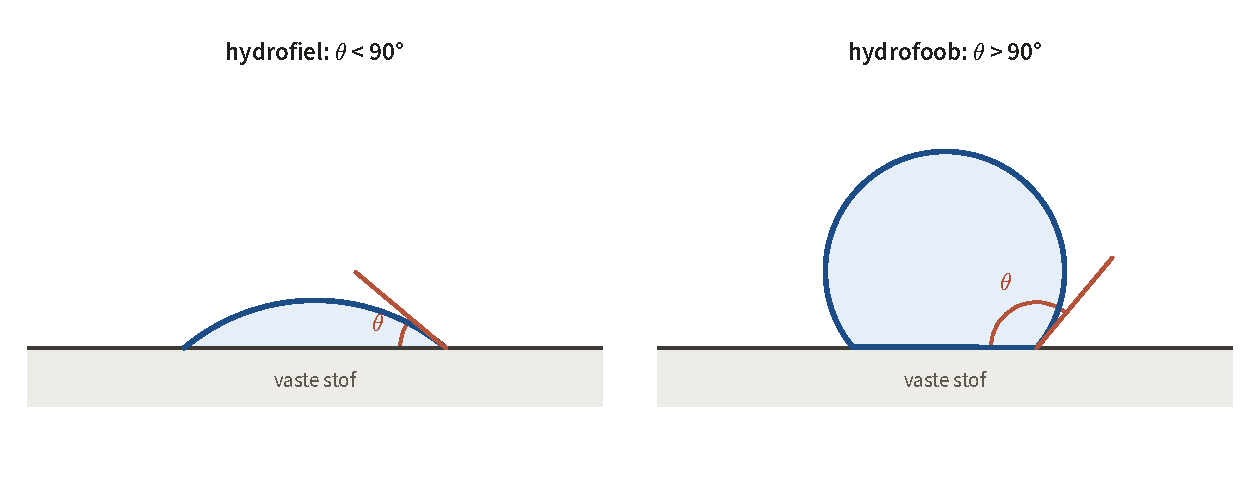
\includegraphics[width=0.85\linewidth]{Figuren/contacthoek}
    \caption{Een druppel op een hydrofiel oppervlak (links, kleine contacthoek) en op een hydrofoob oppervlak (rechts, grote contacthoek). De hoek wordt gemeten door de vloeistof, tussen het vaste oppervlak en de raaklijn aan het vloeistofoppervlak.}
    \label{fig:contacthoek}
\end{figure}

\subsection{Kleine druppels en nauwe poriën: de vergelijking van Kelvin}
\label{sec:kelvin}

Een gekromd oppervlak verandert ook de dampdruk. Een molecule in een kleine druppel staat onder de extra druk $2\sigma/r$ van Young--Laplace; zijn chemische potentiaal stijgt met $V_m\,\Delta p$ (hoofdstuk~\ref{ch:niet-reagerend}). Evenwicht met de damp vraagt dan een hogere dampdruk:
\begin{equation}
\boxed{\;\ln\frac{p}{p_\mathrm{sat}} = \pm\frac{2\sigma V_m}{rRT}\;}
\label{eq:kelvin}
\end{equation}
met het plusteken voor een bolle druppel en het minteken voor een holle meniscus in een porie die bevochtigd wordt. Dit is de \emph{vergelijking van Kelvin}.

\begin{voorbeeld}{Mist, silicagel en een vochtige katalysator}
Voor water bij \SI{20}{\celsius} is $2\sigma V_m/RT = 2(0.072)(\num{1.8e-5})/(8.314\cdot293) = \SI{1.06e-9}{\metre}$.
\begin{itemize}
\item Een druppeltje met $r = \SI{10}{\nano\metre}$: $\ln(p/p_\mathrm{sat}) = 0.106$, dus $p = 1.11\,p_\mathrm{sat}$. Zo'n druppel verdampt in lucht die net verzadigd is. Wolken vormen zich daarom pas op stofdeeltjes of zoutkristalletjes (condensatiekernen), en zuivere lucht kan sterk oververzadigd raken.
\item Een porie met $r = \SI{2}{\nano\metre}$ en volledige bevochtiging: $\ln(p/p_\mathrm{sat}) = -0.53$, dus $p = 0.59\,p_\mathrm{sat}$. Bij een relatieve vochtigheid van \SI{59}{\percent} condenseert water al in zulke poriën. Dat is het werkingsprincipe van silicagel als droogmiddel, en de reden waarom een poreuze katalysatordrager in vochtige lucht water opneemt. Omgekeerd gebruikt men deze \emph{capillaire condensatie} om de poriegrootteverdeling van een materiaal te meten.
\end{itemize}
\end{voorbeeld}

\section{Adsorptie aan grensvlakken}
\label{sec:adsorptie-grensvlakken}

\emph{Adsorptie} is de ophoping van een stof aan een grensvlak, zonder dat ze in de bulk doordringt (dat heet absorptie). Het molecule dat zich hecht, heet het \emph{adsorbaat}; de vaste stof het \emph{adsorbens}. Adsorptie is de eerste stap van elke heterogeen gekatalyseerde reactie (hoofdstuk~\ref{ch:kinetiek}) en de basis van belangrijke scheidingsprocessen: gasdroging, waterzuivering met actieve kool, en de productie van zuivere waterstof, stikstof of zuurstof.

\subsection{Fysisorptie en chemisorptie}
\label{sec:fysisorptie-chemisorptie}

Adsorptie van een molecule aan een oppervlak kan op twee fundamenteel verschillende manieren gebeuren:
\begin{itemize}
\item \textbf{Fysisorptie}: het molecule wordt via zwakke Van der Waals-krachten (hoofdstuk~\ref{ch:intermoleculair}) aan het oppervlak gebonden. De adsorptie-enthalpie is klein (typisch \SIrange{5}{40}{\kilo\joule\per\mole}, vergelijkbaar met een verdampingsenthalpie), niet-specifiek, en kan in meerdere lagen optreden (\S~\ref{sec:bet}). Fysisorptie is snel, reversibel, en neemt toe bij lagere temperatuur.
\item \textbf{Chemisorptie}: het molecule vormt een echte chemische binding (covalent of ionogen, hoofdstuk~\ref{ch:kwantum}) met het oppervlak, vaak gepaard met dissociatie (bijvoorbeeld $\mathrm{H_2}\to2\,\mathrm{H}_{\text{ads}}$). De adsorptie-enthalpie is groot (typisch \SIrange{40}{800}{\kilo\joule\per\mole}), sterk specifiek voor bepaalde oppervlakteatomen, en beperkt tot \'e\'en enkele monolaag. Chemisorptie is de stap die eigenlijk verantwoordelijk is voor katalytische activiteit: de chemische binding tussen reagens en oppervlak verzwakt de interne bindingen van het reagens (bijvoorbeeld de sterke $\mathrm{N\equiv N}$-binding bij Haber--Bosch), wat exact de activeringsenergie van de daaropvolgende reactiestap verlaagt.
\end{itemize}
Beide vormen van adsorptie zijn, net als elke andere fase-overgang (hoofdstuk~\ref{ch:niet-reagerend}), exotherm: een molecule dat zich aan een oppervlak bindt, verliest bewegingsvrijheid (negatieve adsorptie-entropie, hoofdstuk~\ref{ch:spontaniteit}), zodat enkel een negatieve adsorptie-enthalpie een spontaan ($\Delta G_{\text{ads}}<0$) proces kan opleveren.

\subsection{Het adsorptie-evenwicht en de Langmuir-isotherme}
\label{sec:langmuir-isotherm-kinetiek}

Om adsorptie en later de kinetiek van een oppervlaktereactie te beschrijven, hebben we een kwantitatieve uitdrukking nodig voor de \emph{bedekkingsgraad} $\theta$ van het oppervlak: de fractie van de beschikbare adsorptieplaatsen die bezet is, met $0\leq\theta\leq1$.

Beschouw een gas $A$ met partiële druk $p_A$ boven een oppervlak met een vast aantal adsorptieplaatsen. We veronderstellen (het model van \emph{Langmuir}):
\begin{itemize}
\item alle adsorptieplaatsen zijn energetisch equivalent;
\item elke plaats kan hoogstens \'e\'en molecule dragen (monolaagadsorptie);
\item geadsorbeerde moleculen be\"invloeden elkaar niet.
\end{itemize}
De snelheid van adsorptie is evenredig met zowel de partiële druk (botsingsfrequentie met het oppervlak) als de fractie \emph{vrije} plaatsen $(1-\theta)$:
\[
r_{\text{ads}} = k_a\,p_A\,(1-\theta).
\]
De snelheid van desorptie is evenredig met de fractie \emph{bezette} plaatsen:
\[
r_{\text{des}} = k_d\,\theta.
\]
In evenwicht zijn beide snelheden gelijk, $r_{\text{ads}}=r_{\text{des}}$:
\[
k_a\,p_A(1-\theta) = k_d\,\theta \quad\Longrightarrow\quad \theta = \frac{k_a\,p_A}{k_d+k_a\,p_A}.
\]
Met de \emph{adsorptie-evenwichtsconstante} $K_A\equiv k_a/k_d$ (met dimensie druk$^{-1}$) volgt de \emph{Langmuir-isotherme}:
\begin{equation}
\boxed{\;\theta_A = \frac{K_A\,p_A}{1+K_A\,p_A}.\;}
\label{eq:langmuir-isotherm}
\end{equation}
Bij lage druk ($K_Ap_A\ll1$) is $\theta_A\approx K_Ap_A$: de bedekking stijgt lineair met de druk. Bij hoge druk ($K_Ap_A\gg1$) is $\theta_A\to1$: het oppervlak is volledig verzadigd en verdere drukverhoging heeft nauwelijks effect --- hetzelfde verzadigingsgedrag dat in hoofdstuk~\ref{ch:kinetiek} terugkomt bij enzymen (Michaelis--Menten).

Voor twee competitief adsorberende gassen $A$ en $B$ geldt op dezelfde manier:
\begin{equation}
\theta_A = \frac{K_Ap_A}{1+K_Ap_A+K_Bp_B}, \qquad \theta_B = \frac{K_Bp_B}{1+K_Ap_A+K_Bp_B}.
\label{eq:langmuir-competitief}
\end{equation}
Een sterker adsorberende component (grotere $K$) verdringt een zwakker adsorberende component van het oppervlak Dat effect bepaalt de snelheid van oppervlaktereacties (hoofdstuk~\ref{ch:kinetiek}) en het vergiftigen van katalysatoren, bijvoorbeeld door CO op het platina van een brandstofcel.

De constante $K$ is een evenwichtsconstante en volgt dus de vergelijking van Van 't Hoff (hoofdstuk~\ref{ch:reagerend}): omdat adsorptie exotherm is, daalt $K$ bij stijgende temperatuur. Een adsorbens laadt men daarom koud en onder druk, en regenereert men warm of bij lage druk.

\begin{toepassing}{Zuivere waterstof met drukwisseladsorptie (PSA)}
Na de stoomreformer en de shiftreactoren (hoofdstuk~\ref{ch:reagerend}, \S~\ref{sec:case-waterstof}) bevat het gas ongeveer \SI{75}{\percent} H$_2$, de rest is vooral CO$_2$, met wat CH$_4$, CO en water. In een PSA-eenheid stroomt dit gas bij ongeveer \SI{25}{\bar} door kolommen met actieve kool en zeoliet. CO$_2$, CH$_4$ en CO adsorberen sterk (grote $K$), H$_2$ nauwelijks: het verlaat de kolom met een zuiverheid van \SI{99.999}{\percent}. Is een kolom vol, dan laat men de druk zakken tot net boven \SI{1}{\bar}: volgens de Langmuir-isotherme komt het grootste deel van het adsorbaat weer vrij. Enkele kolommen wisselen elkaar af in cycli van enkele minuten. Hetzelfde principe levert stikstof uit lucht (koolstofmoleculaire zeven) en zuurstof voor zuurstofconcentrators in de zorg (zeolieten die N$_2$ sterker binden dan O$_2$).
\end{toepassing}

\begin{figure}[htb]
    \centering
    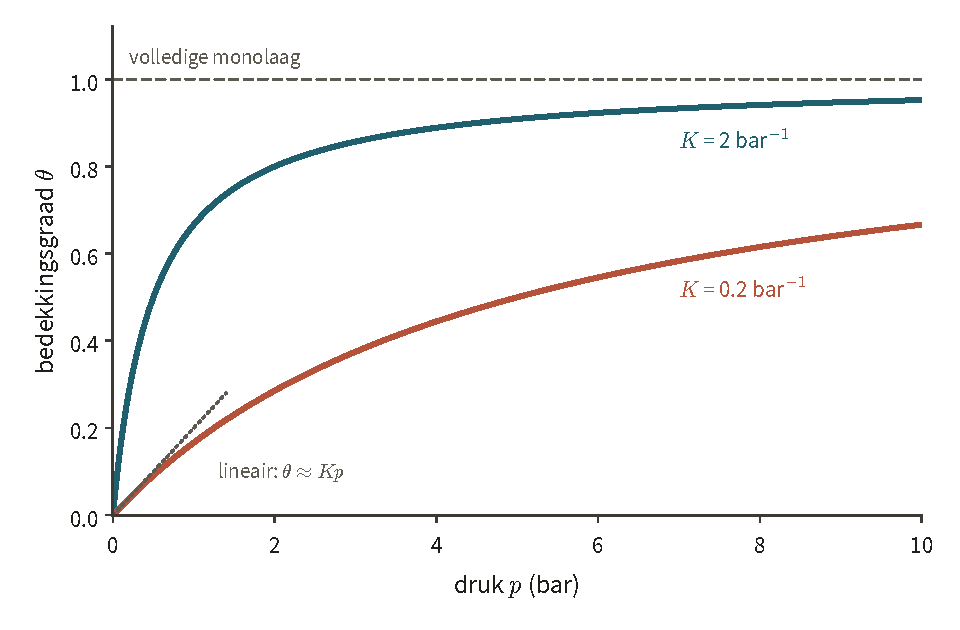
\includegraphics[width=0.7\linewidth]{Figuren/langmuir_isotherm}
    \caption{De Langmuir-isotherme (vergelijking~\eqref{eq:langmuir-isotherm}) voor twee waarden van de adsorptieconstante. Bij lage druk stijgt de bedekking lineair, bij hoge druk nadert ze een volledige monolaag. Een sterker adsorberend gas (grotere $K$) verzadigt het oppervlak al bij lage druk.}
    \label{fig:langmuir-isotherm}
\end{figure}

\subsection{De BET-isotherme: voorbij de monolaag}
\label{sec:bet}

De Langmuir-isotherme veronderstelt monolaagadsorptie --- gerechtvaardigd voor chemisorptie, maar niet voor fysisorptie, waar bij voldoende hoge relatieve druk meerdere lagen fysisorberen (vergelijkbaar met condensatie, hoofdstuk~\ref{ch:niet-reagerend}). Brunauer, Emmett en Teller (1938) breidden het Langmuir-model uit tot multilaagadsorptie, wat leidt tot de \emph{BET-isotherme}:
\begin{equation}
\frac{V}{V_m} = \frac{C\,x}{(1-x)\bigl[1-x+Cx\bigr]}, \qquad x=\frac{p}{p_{\text{sat}}},
\label{eq:bet}
\end{equation}
waarin $V$ het geadsorbeerde volume, $V_m$ het volume van precies \'e\'en monolaag, $p_{\text{sat}}$ de verzadigingsdampdruk van het adsorberende gas bij de gegeven temperatuur (hoofdstuk~\ref{ch:niet-reagerend}), en $C$ een constante gerelateerd aan het verschil tussen de adsorptie-enthalpie van de eerste laag en de condensatie-enthalpie van de volgende lagen. De BET-vergelijking wordt industrieel op grote schaal gebruikt om, via stikstofadsorptie bij \SI{77}{\kelvin}, het specifieke oppervlak (\si{\metre\squared\per\gram}) van poreuze katalysatoren te bepalen ($V_m$ levert immers rechtstreeks het aantal adsorptieplaatsen, en dus het oppervlak, op) --- een routinematige, onmisbare karakterisatietechniek voor elke heterogene katalysator.

In de praktijk gebruikt men de gelineariseerde vorm
\begin{equation}
\frac{x}{V(1-x)} = \frac{1}{V_mC} + \frac{C-1}{V_mC}\,x ,
\label{eq:bet-lineair}
\end{equation}
die in het gebied $x = 0.05$--$0.30$ een rechte geeft. Uit helling en asafsnede volgen $V_m$ en $C$. Elk stikstofmolecule in de monolaag neemt ongeveer \SI{0.162}{\nano\metre\squared} in, zodat
\begin{equation}
a_s = \frac{V_m}{\SI{22414}{\centi\metre\cubed\per\mole}}\,N_A\,(\SI{0.162e-18}{\metre\squared}) = \SI{4.35}{\metre\squared\per\gram}\ \text{per}\ \si{\centi\metre\cubed}\,(\mathrm{STP})/\si{\gram}\ \text{monolaag}.
\label{eq:bet-oppervlak}
\end{equation}

\begin{figure}[htb]
    \centering
    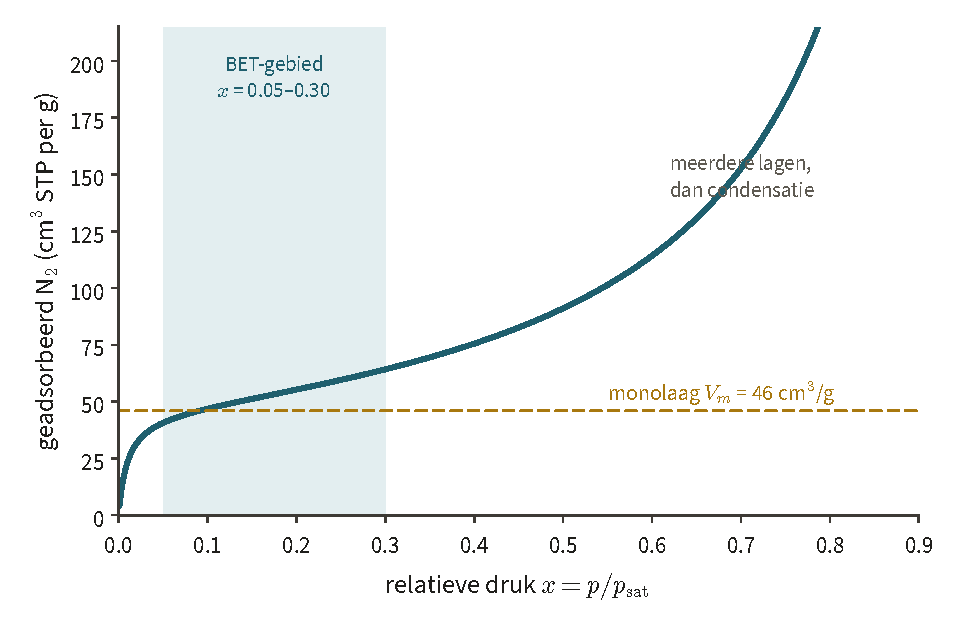
\includegraphics[width=0.7\linewidth]{Figuren/bet_isotherm}
    \caption{Stikstofadsorptie bij \SI{77}{\kelvin} op een poreuze drager (BET-model met $C = 100$ en $V_m = \SI{46}{\centi\metre\cubed\per\gram}$). Rond $x \approx 0.1$ is de eerste laag vol; daarna groeien meer lagen en volgt capillaire condensatie in de poriën.}
    \label{fig:bet-isotherm}
\end{figure}

\begin{voorbeeld}{Het oppervlak van de katalysatordrager}
Voor de $\gamma$-$\mathrm{Al_2O_3}$-korrel van de centrale case levert de BET-rechte $V_m = \SI{46}{\centi\metre\cubed}$ (STP) per gram. Met vergelijking~\eqref{eq:bet-oppervlak}: $a_s = 46 \times 4.35 = \SI{200}{\metre\squared\per\gram}$. Een korrel van \SI{1}{\gram} heeft dus een inwendig oppervlak van \SI{200}{\metre\squared}, terwijl de buitenkant van die korrel nog geen \SI{5}{\centi\metre\squared} meet. Vergelijk met vergelijking~\eqref{eq:specifiek-oppervlak}: zonder poriën zouden de korrels kleiner dan \SI{10}{\nano\metre} moeten zijn.
\end{voorbeeld}

\subsection{Adsorptie uit een oplossing}
\label{sec:adsorptie-oplossing}

Ook opgeloste stoffen adsorberen: kleurstoffen, pesticiden of geurstoffen op actieve kool, eiwitten op een membraan. Het adsorbens is dan zelden homogeen genoeg voor Langmuir, en men gebruikt vaak de empirische \emph{Freundlich-isotherme}
\begin{equation}
q = K_F\,c^{1/n},
\label{eq:freundlich}
\end{equation}
met $q$ de geadsorbeerde hoeveelheid per kg adsorbens, $c$ de concentratie in oplossing en $n > 1$. Op een log--logschaal is dat een rechte. Zoals bij gasadsorptie geldt: hydrofobe, slecht oplosbare moleculen adsorberen het sterkst op hydrofobe kool (hoofdstuk~\ref{ch:intermoleculair}, \S~\ref{sec:im-toepassingen}).

\section{Surfactanten en micelvorming}
\label{sec:surfactanten}

\emph{Surfactanten} (oppervlakte-actieve stoffen) zijn moleculen met een dualistische structuur: een hydrofiele kop en een hydrofobe staart. In water accumuleren zij aan het vloeistof--luchtgrensvlak, met de hydrofobe staart naar de lucht gericht. Hierdoor wordt de oppervlaktespanning sterk verlaagd.

\subsection{De kritische micelconcentratie (CMC)}

Boven een bepaalde concentratie, de \emph{kritische micelconcentratie} (CMC), organiseren surfactanten zich spontaan in aggregaten: \emph{micellen}. In een micel zijn de hydrofobe staarten naar binnen gericht en de hydrofiele koppen naar buiten, zodat het micel als geheel wateroplosbaar is. Onder de CMC gedragen surfactanten zich als gewone opgeloste stoffen; boven de CMC blijft de concentratie vrije surfactant constant en worden bijkomende moleculen in micellen opgenomen.

\begin{voorbeeld}{CMC van natriumdodecylsulfaat}
Natriumdodecylsulfaat (SDS, $\mathrm{CH_3(CH_2)_{11}OSO_3Na}$) heeft een CMC van \SI{8.2e-3}{\mole\per\litre} bij \SI{25}{\celsius}. Onder deze concentratie daalt de oppervlaktespanning geleidelijk met de SDS-concentratie; boven de CMC blijft de oppervlaktespanning constant op ongeveer \SI{35}{\milli\newton\per\metre}. Dit is een direct gevolg van de micelvorming: bijkomende SDS verhoogt enkel het aantal micellen, niet de concentratie vrije surfactant.
\end{voorbeeld}

\subsection{Thermodynamica van micelvorming}

Micelvorming is een spontaan proces met een negatieve Gibbs-energie. De drijvende kracht is de entropie: de waterstructuur rond de hydrofobe staarten (``ijskragen'') wordt verbroken wanneer de staarten zich in een micel samenpakken. Dit \emph{hydrofoob effect} is entropisch van aard, een directe illustratie van de principes uit hoofdstuk~\ref{ch:spontaniteit} (\S~\ref{sec:waarschijnlijkheid-entropie}).

\begin{toepassing}{Tweede case: hoe een wasmiddel vet verwijdert}
Een vetvlek op katoen is hydrofoob en bevochtigt het water slecht. Surfactanten in het wasmiddel adsorberen met hun staart aan het vet en met hun kop naar het water: de grensvlakspanning vet--water daalt van ongeveer \SI{50}{\milli\newton\per\metre} tot enkele \si{\milli\newton\per\metre}. Daardoor verandert de contacthoek (vergelijking~\eqref{eq:young}) en rolt het vet op tot druppeltjes die loskomen van de vezel. Boven de CMC worden die druppeltjes in micellen opgenomen; de geladen koppen houden ze uit elkaar (\S~\ref{sec:colloiden}). Warmer water helpt, omdat vet vloeibaarder wordt en de oppervlaktespanning daalt, maar moderne enzymen en surfactanten werken al bij \SI{30}{\celsius}, wat veel energie bespaart.
\end{toepassing}

\section{Collo\"idale dispersies en stabiliteit}
\label{sec:colloiden}

Een \emph{collo\"ide} is een dispersie van deeltjes met een grootte tussen \SI{1}{\nano\metre} en \SI{1}{\micro\metre} in een continue fase. Voorbeelden: emulsies (melk, mayonaise), suspensies (verf), schuimen (bier), aerosolen (mist). Collo\"idale deeltjes zijn groot genoeg om Brownse beweging te vertonen, maar klein genoeg om niet snel te sedimenteren.

\subsection{Het potentieel van DLVO}
\label{sec:dlvo}

De stabiliteit van een collo\"idale dispersie wordt bepaald door de balans tussen twee krachten:
\begin{itemize}
\item \textbf{Van der Waals-aantrekking} (hoofdstuk~\ref{ch:intermoleculair}): brengt deeltjes samen en leidt tot coagulatie.
\item \textbf{Elektrostatische afstoting}: ontstaat door geladen oppervlakken met een elektrische dubbellaag; werkt de aantrekking tegen.
\end{itemize}
De som van beide krachten als functie van de afstand vormt de \emph{potenti\"ele energiecurve} van DLVO (Derjaguin--Landau--Verwey--Overbeek). Bij voldoende afstoting ontstaat een energiedrempel die coagulatie verhindert; de dispersie is dan kinetisch stabiel (figuur~\ref{fig:dlvo}). Voegt men zout toe, dan wordt de afstoting korter van bereik en verdwijnt de drempel.

\begin{figure}[htb]
    \centering
    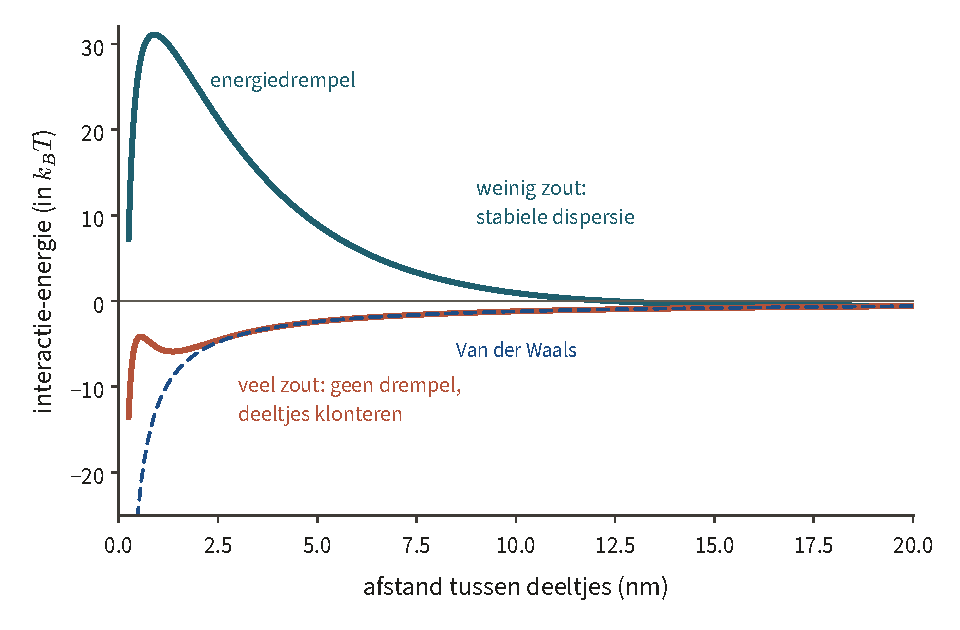
\includegraphics[width=0.7\linewidth]{Figuren/dlvo}
    \caption{DLVO-energie tussen twee colloïdale deeltjes (schematisch): de som van een Van der Waals-aantrekking en een elektrostatische afstoting. Bij weinig zout is er een drempel van tientallen $k_BT$ en blijft de dispersie stabiel; bij veel zout verdwijnt de drempel en klonteren de deeltjes samen.}
    \label{fig:dlvo}
\end{figure}

\subsection{De elektrische dubbellaag}

In waterige oplossingen krijgen collo\"idale deeltjes een oppervlaktelading door ionisatie van oppervlaktegroepen, adsorptie van ionen (\S~\ref{sec:adsorptie-grensvlakken}) of isomorfe substitutie. Deze lading wordt gecompenseerd door een tegenionenwolk: de \emph{elektrische dubbellaag}. Het model van Gouy--Chapman--Stern beschrijft twee gebieden:
\begin{enumerate}
\item Een \emph{Stern-laag}: stevig gebonden tegenionen dicht bij het oppervlak.
\item Een \emph{diffuse laag}: een wolk van tegenionen met geleidelijk afnemende concentratie, die in de bulk overgaat.
\end{enumerate}
Het potentiaalverloop in de diffuse laag is exponentieel, met karakteristieke lengte $\kappa^{-1}$ (Debye-lengte). In water bij \SI{25}{\celsius} geldt voor een 1:1-zout $\kappa^{-1} \approx \SI{0.304}{\nano\metre}/\sqrt{c/(\si{\mole\per\litre})}$: ongeveer \SI{10}{\nano\metre} in zoet water ($c \approx \SI{1}{\milli\mole\per\litre}$), maar slechts \SI{0.4}{\nano\metre} in zeewater. Dat verklaart waarom rivierslib neerslaat zodra de rivier de zee bereikt: de delta's van de Schelde en de Nijl zijn ook een colloïdchemisch verschijnsel.

\subsection{De zeta-potentiaal}

Het praktisch meetbare potentiaal aan de grens tussen de Stern-laag en de diffuse laag is de \emph{zeta-potentiaal} $\zeta$. Een collo\"ide met $|\zeta| > \SI{30}{\milli\volt}$ is doorgaans stabiel; bij $|\zeta| < \SI{10}{\milli\volt}$ coaguleert de dispersie snel.

\begin{voorbeeld}{Zeta-potentiaal en waterzuivering}
In waterzuiveringsinstallaties worden collo\"idale deeltjes (klei, organisch materiaal) verwijderd door coagulatie. Door toevoeging van $\mathrm{Al_2(SO_4)_3}$ of $\mathrm{FeCl_3}$ wordt de zeta-potentiaal verlaagd: de veelwaardige kationen ($\mathrm{Al^{3+}}$, $\mathrm{Fe^{3+}}$) comprimeren de dubbellaag en reduceren $\zeta$. Hierdoor verliest het collo\"ide zijn stabiliteit en slaat het neer. Dit is het werkingsmechanisme van flocculatie in drinkwaterproductie.
\end{voorbeeld}

\subsection{Elektrokinetische verschijnselen}

Wanneer een collo\"ide met geladen oppervlak zich in een elektrisch veld bevindt, kunnen twee verschijnselen optreden:
\begin{itemize}
\item \textbf{Elektroforese}: de deeltjes bewegen naar de tegengesteld geladen elektrode.
\item \textbf{Elektro-osmose}: de vloeistof beweegt langs een geladen vaste wand wanneer een elektrisch veld wordt aangelegd.
\end{itemize}
Beide verschijnselen worden beschreven door de vergelijking van Smoluchowski en worden toegepast in inktprinters, elektroforetische coatings, DNA-scheiding en microfluidica.

\section{Emulsies en stabilisatoren}
\label{sec:emulsies}

Een \emph{emulsie} is een dispersie van een vloeistof in een andere onmengbare vloeistof. Twee types worden onderscheiden:
\begin{itemize}
\item \textbf{Olie-in-water (O/W)}: oliedruppels in waterige fase (melk, mayonaise, cosmeticum).
\item \textbf{Water-in-olie (W/O)}: waterdruppels in oliefase (boter, margarine, sommige zalven).
\end{itemize}
Emulsies zijn thermodynamisch onstabiel (de Gibbs-energie van de grensvlakken is positief), maar kunnen kinetisch stabiel worden gemaakt door \emph{emulgatoren}: surfactanten of vaste deeltjes die zich aan het vloeistof--vloeistofgrensvlak hechten en een beschermende laag vormen.

\subsection{Het HLB-getal}

De keuze van de juiste surfactant voor een emulsie wordt geholpen door het \emph{HLB-getal} (Hydrofiel--Lipofiel Balans):
\begin{itemize}
\item HLB 3--6: W/O-emulgator.
\item HLB 8--18: O/W-emulgator.
\end{itemize}
Voor mayonaise (O/W) gebruikt men bijvoorbeeld eiwit (HLB $\sim$ 13); voor margarine (W/O) gebruikt men mono- en diglyceriden (HLB $\sim$ 4).

\section{Schuimen en antischuimmiddelen}

Een \emph{schuim} is een dispersie van gas in vloeistof. Schuimen zijn kinetisch stabiel door surfactanten die de gasbel-wanden versterken (Marangoni-effect: herstel van lokale oppervlaktespanningsgradi\"enten). Schuimen zijn gewenst in bier, scheerschuim en brandblusschuim, maar ongewenst in fermentoren, destillatiekolommen en waswater.

\emph{Antischuimmiddelen} werken door de lokale oppervlaktespanning sterk te verlagen of door de film te verzwakken. Vaak gebruikt men siliconenoli\"e\"en of hydrofoob silica.

\section{De vaste stof: van atomen naar kristallen}
\label{sec:vaste-stof}

Het oppervlak waarop alles in dit hoofdstuk gebeurt, hoort bij een vaste stof. Een katalysatordrager, een elektrode, een pigment of een zeoliet heeft eigenschappen die rechtstreeks volgen uit hoe de atomen gerangschikt zijn: in een regelmatig kristal, met defecten, of amorf. Voor de chemisch ingenieur is de vaste stof dus veel meer dan een passieve drager: de kristalstructuur bepaalt de katalytische activiteit, de elektronenstructuur ligt aan de basis van zonnecellen en led's, en defecten bepalen de sterkte en de corrosie van constructiematerialen.

\subsection{Kristalstructuren: de Bravais-roosters}
\label{sec:bravais}

Een \emph{kristal} is een vaste stof waarin de atomen in een regelmatige, driedimensionale rangschikking zijn geordend. Deze rangschikking wordt beschreven door een \emph{kristalrooster}: een oneindige herhaling van een elementaire cel langs drie onafhankelijke richtingen.

\subsubsection{De elementaire cel}

De \emph{elementaire cel} is de kleinste eenheid die, door herhaling in drie richtingen, het volledige kristal opbouwt. Zij wordt gekenmerkt door drie roosterconstanten $a$, $b$, $c$ (lengtes) en drie hoeken $\alpha$, $\beta$, $\gamma$ (tussen de assen).

Er bestaan precies \emph{14} onafhankelijke roostertypes, de \emph{Bravais-roosters}, verdeeld over 7 kristalsystemen:
\begin{itemize}
\item \textbf{Kubisch}: primitief (P), ruimtelijk gecentreerd (I), vlakgecentreerd (F).
\item \textbf{Tetragonaal}: primitief, ruimtelijk gecentreerd.
\item \textbf{Orthorombisch}: primitief, ruimtelijk gecentreerd, vlakgecentreerd, basaal gecentreerd.
\item \textbf{Hexagonaal}: primitief.
\item \textbf{Trigonaal} (rhombohedrisch): primitief.
\item \textbf{Monoclien}: primitief, basaal gecentreerd.
\item \textbf{Triklien}: primitief.
\end{itemize}
Tel je deze op (3+2+4+1+1+2+1), dan kom je inderdaad op precies 14 uit: geen enkel ander roostertype is met een periodieke driedimensionale rangschikking van punten verenigbaar.

\subsubsection{De drie kubische roosters}

De eenvoudigste en belangrijkste roosters voor metallische en ionische vaste stoffen zijn de drie kubische types:

\begin{itemize}
\item \textbf{Primitief kubisch (P)}: atomen op de 8 hoeken van een kubus. Aantal atomen per cel: $8 \times \tfrac{1}{8} = 1$.
\item \textbf{Ruimtelijk gecentreerd kubisch (BCC, I)}: bijkomend atoom in het centrum. Aantal atomen per cel: $1 + 1 = 2$.
\item \textbf{Vlakgecentreerd kubisch (FCC, F)}: bijkomend atoom op elk van de 6 vlakken (gedeeld door 2 cellen). Aantal atomen per cel: $1 + 6 \times \tfrac{1}{2} = 4$.
\end{itemize}

\begin{figure}[htb]
    \centering
    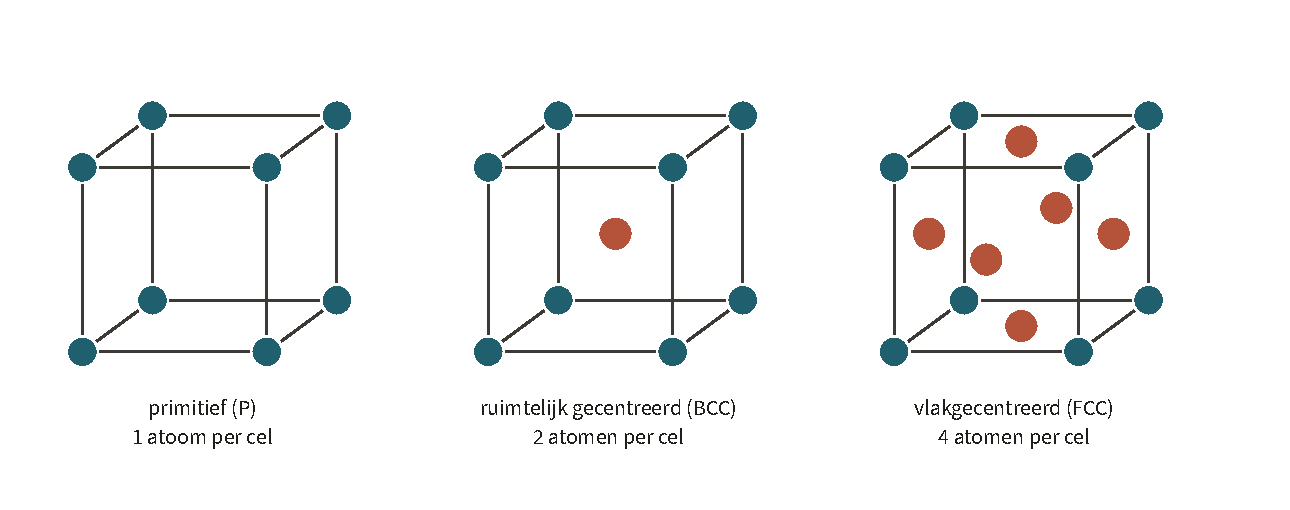
\includegraphics[width=0.95\linewidth]{Figuren/kubische_roosters}
    \caption{De drie kubische Bravais-roosters: primitief kubisch (enkel hoekatomen), ruimtelijk gecentreerd (BCC, met een atoom in het centrum) en vlakgecentreerd (FCC, met een atoom op elk van de zes vlakken). Een hoekatoom wordt gedeeld door acht cellen, een vlakatoom door twee.}
    \label{fig:kubische-roosters}
\end{figure}

\begin{voorbeeld}{Pakking en atoomradius in FCC}
In een FCC-rooster (bv. Cu, Al, $\gamma$-Fe) raken de atomen langs de diagonaal van een vlak. Met roosterconstante $a$ geldt $4r = a\sqrt{2}$, zodat $r = a\sqrt{2}/4$. Voor koper met $a = \SI{0.361}{\nano\metre}$:
\[
r = \frac{\SI{0.361}{\nano\metre}\,\sqrt{2}}{4} = \SI{0.128}{\nano\metre}.
\]
De pakking (fractie van het volume ingenomen door atomen) bedraagt $\pi/(3\sqrt{2}) \approx 0.74$ --- de dichtst mogelijke bolpakking.
\end{voorbeeld}

\subsubsection{Structuren van ionische en covalente vaste stoffen}

Enkele veelvoorkomende structuurtypen:

\begin{itemize}
\item \textbf{NaCl-structuur}: FCC-rooster van $\mathrm{Cl^-}$ met $\mathrm{Na^+}$ in alle octa\"edrische holtes. Co\"ordinatiegetal 6:6.
\item \textbf{CsCl-structuur}: primitief kubisch rooster van $\mathrm{Cl^-}$ met $\mathrm{Cs^+}$ in het lichaam-centrum. Co\"ordinatiegetal 8:8.
\item \textbf{Zinkblende (ZnS)}: FCC-rooster van $\mathrm{S^{2-}}$ met $\mathrm{Zn^{2+}}$ in de helft van de tetra\"edrische holtes. Co\"ordinatie 4:4. Belangrijk voor halfgeleiders (GaAs, CdTe).
\item \textbf{Fluoriet ($\mathrm{CaF_2}$)}: FCC-rooster van $\mathrm{Ca^{2+}}$ met $\mathrm{F^-}$ in alle tetra\"edrische holtes. Belangrijk voor $\mathrm{UO_2}$, $\mathrm{CeO_2}$, $\mathrm{ZrO_2}$.
\item \textbf{Diamant}: FCC-rooster met twee interpenetrerende subroosters, elk atoom tetra\"edrisch omringd. Dit is de structuur van Si, Ge, C (diamant).
\end{itemize}

\subsection{R\"ontgendiffractie en de wet van Bragg}
\label{sec:xrd}

De experimentele methode bij uitstek voor de bepaling van kristalstructuren is \emph{r\"ontgendiffractie} (XRD). De golflengte van r\"ontgenstraling (\SIrange{0.1}{1}{\angstrom}) is van dezelfde orde als interatomaire afstanden, zodat diffractie optreedt aan de roostervlakken.

\subsubsection{Millerindices: het aanduiden van roostervlakken}
\label{sec:miller}

Om een specifieke set evenwijdige roostervlakken ondubbelzinnig aan te duiden, gebruikt men \emph{Millerindices} $(hkl)$: drie gehele getallen, bepaald door de omgekeerde waarden van de snijpunten van het vlak met de drie kristalassen (uitgedrukt in eenheden van de roosterconstanten $a$, $b$, $c$) te nemen en tot de kleinste gehele verhouding te herleiden. Een vlak dat de $x$-, $y$- en $z$-as elk op afstand $a$ snijdt, heeft dus Millerindices $(111)$; een vlak evenwijdig met de $y$- en $z$-as (het snijdt enkel de $x$-as) heeft indices $(100)$.

Voor een \emph{kubisch} rooster met roosterconstante $a$ is de afstand tussen opeenvolgende $(hkl)$-vlakken:
\begin{equation}
\boxed{\;d_{hkl} = \frac{a}{\sqrt{h^2+k^2+l^2}}.\;}
\label{eq:dhkl}
\end{equation}
Voor de $(111)$-vlakken geeft dit bijvoorbeeld $d_{111}=a/\sqrt{1^2+1^2+1^2}=a/\sqrt3$ --- de relatie die we hieronder gebruiken om, via de wet van Bragg, de roosterconstante van koper te bepalen. Deze combinatie --- Millerindices om een vlak te identificeren, vergelijking~\eqref{eq:dhkl} om de bijhorende vlakafstand te berekenen, en de wet van Bragg (hieronder) om die vlakafstand experimenteel te meten --- vormt samen het volledige gereedschap om een onbekende kubische kristalstructuur te karakteriseren.

\subsubsection{De wet van Bragg}
\label{sec:bragg}

Wanneer een r\"ontgenbundel invalt op een kristal onder hoek $\theta$ ten opzichte van een set roostervlakken met intervlakafstand $d$, treden versterkende interferenties op wanneer:
\begin{equation}
\boxed{\;n\lambda = 2\,d\,\sin\theta\;}
\label{eq:bragg}
\end{equation}
waarin $\lambda$ de golflengte en $n$ een geheel getal is (de ``orde''). Uit de gemeten hoeken $\theta$ kan $d$ worden berekend via vergelijking~\eqref{eq:dhkl}, en uit het volledige diffractiepatroon de kristalstructuur worden gereconstrueerd.

\begin{figure}[htb]
    \centering
    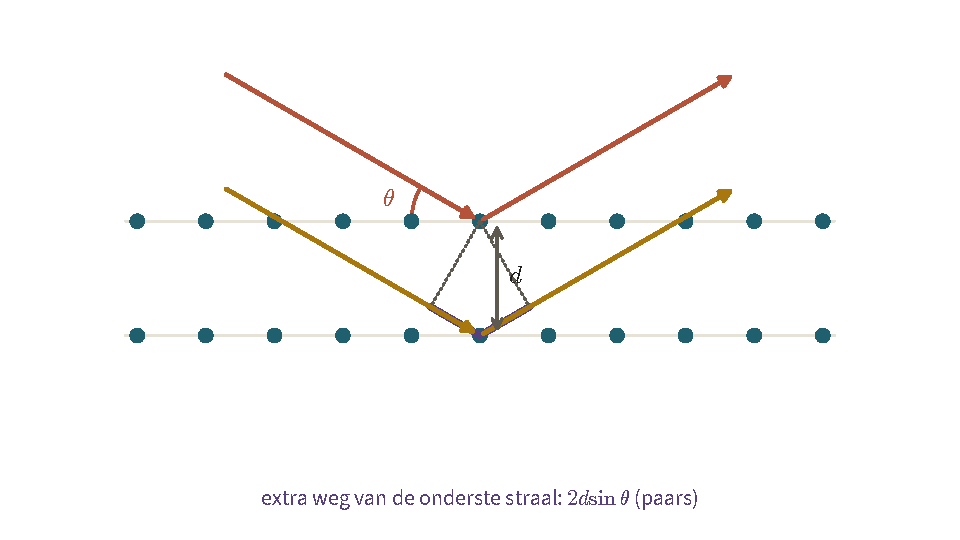
\includegraphics[width=0.75\linewidth]{Figuren/bragg_geometrie}
    \caption{Braggdiffractie aan twee evenwijdige roostervlakken op afstand $d$. De straal die het onderste vlak treft, legt een extra weg $2d\sin\theta$ af. Enkel als dat een geheel aantal golflengten is, versterken de gereflecteerde stralen elkaar (vergelijking~\eqref{eq:bragg}).}
    \label{fig:bragg-geometrie}
\end{figure}

\begin{voorbeeld}{Bepaling van de roosterconstante van koper --- let op $2\theta$ versus $\theta$}
Een veelvoorkomende valkuil bij het praktisch gebruik van de wet van Bragg is de volgende: XRD-toestellen rapporteren doorgaans de hoek $2\theta$ tussen de invallende en de gediffracteerde bundel (de hoek waarover de detector effectief draait), \emph{niet} de hoek $\theta$ uit vergelijking~\eqref{eq:bragg} zelf, die ten opzichte van het roostervlak wordt gemeten. Het rechtstreeks invullen van een gerapporteerde $2\theta$-waarde als $\theta$ levert een systematisch verkeerd resultaat op.

Een poederdiffractiepatroon van koper ($\lambda = \SI{0.154}{\nano\metre}$, Cu K$\alpha$) toont een eerste piek bij $2\theta = 43.1^\circ$, dus $\theta = 21.55^\circ$. Voor de $(111)$-vlakken geeft de wet van Bragg ($n=1$):
\[
d_{111} = \frac{\lambda}{2\sin\theta} = \frac{\SI{0.154}{\nano\metre}}{2\sin(21.55^\circ)} = \frac{\SI{0.154}{\nano\metre}}{0.7337} \approx \SI{0.210}{\nano\metre}.
\]
Met vergelijking~\eqref{eq:dhkl}, $d_{111} = a/\sqrt{3}$ voor een kubisch rooster:
\[
a = d_{111}\sqrt{3} \approx (\SI{0.210}{\nano\metre})(1.732) \approx \SI{0.363}{\nano\metre},
\]
in uitstekende overeenstemming met de bekende roosterconstante van Cu ($a=\SI{0.3615}{\nano\metre}$, reeds gebruikt in \S~\ref{sec:bravais}). Zou men $43.1^\circ$ ten onrechte rechtstreeks als $\theta$ hebben ingevuld, dan volgt $d_{111}\approx\SI{0.113}{\nano\metre}$ en $a\approx\SI{0.195}{\nano\metre}$ --- bijna een factor twee te klein, en duidelijk onverenigbaar met de bekende dichtheid en atoomstraal van koper. Controleer daarom bij elke XRD-analyse expliciet of de gerapporteerde hoek $\theta$ dan wel $2\theta$ voorstelt, vooraleer de wet van Bragg toe te passen.
\end{voorbeeld}

\subsubsection{Het poederdiffractiepatroon}

In plaats van een enkelkristal wordt in de praktijk vaak een poeder gebruikt, zodat alle mogelijke vlakori\"entaties simultaan aanwezig zijn. Het resulterende \emph{poederdiffractiepatroon} (XRD-patroon) is een reeks pieken bij verschillende $2\theta$. De positie van de pieken geeft de roosterconstanten; de intensiteit geeft de atoomposities binnen de cel; de breedte geeft informatie over korrelgrootte en defecten.

\begin{figure}[htb]
    \centering
    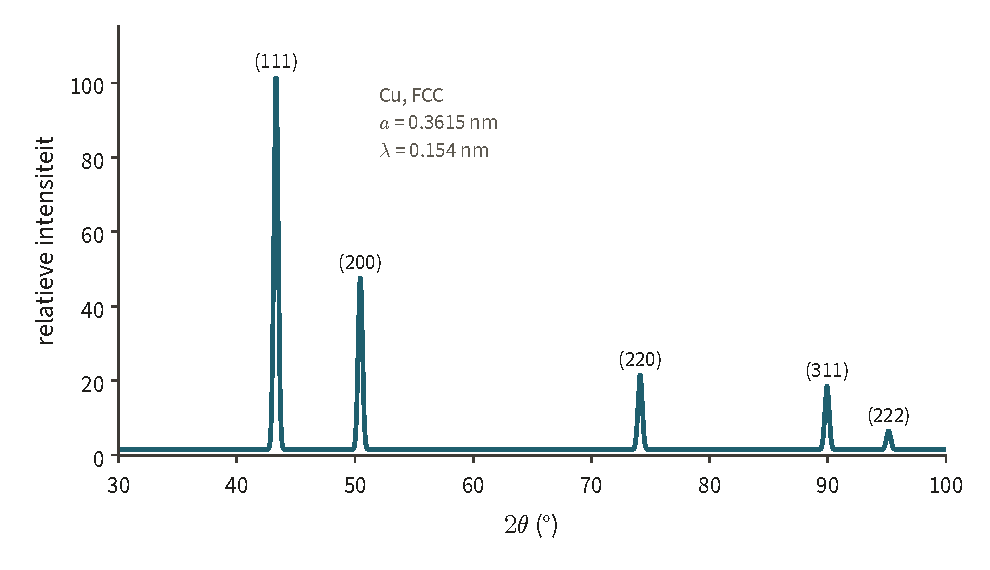
\includegraphics[width=0.75\linewidth]{Figuren/xrd_poederpatroon}
    \caption{Berekend poederdiffractogram van koper (FCC, $a = \SI{0.3615}{\nano\metre}$, Cu K$\alpha$-straling). In een FCC-rooster zijn enkel reflecties zichtbaar waarvoor $h$, $k$ en $l$ allemaal even of allemaal oneven zijn. Elke piekpositie geeft via de wet van Bragg en vergelijking~\eqref{eq:dhkl} de roosterconstante.}
    \label{fig:xrd-poederpatroon}
\end{figure}

Vergelijking met databanken (JCPDS, ICDD) laat toe een onbekende stof in seconden te identificeren. Dit is standaard in katalysatorkarakterisatie, kwaliteitscontrole, forensische chemie en farmaceutische analyse (polymorfie).

Ook de \emph{breedte} van een piek is nuttig. Een oneindig groot kristal geeft een scherpe piek; een kristalletje van enkele nanometer heeft te weinig roostervlakken om buiten de Braggvoorwaarde volledig uit te doven, en geeft een brede piek. De \emph{vergelijking van Scherrer} schat de kristalgrootte $\tau$:
\begin{equation}
\tau = \frac{K\lambda}{\beta\cos\theta},
\label{eq:scherrer}
\end{equation}
met $K \approx 0.9$ en $\beta$ de piekbreedte op halve hoogte, in radialen op de $2\theta$-schaal.

\begin{voorbeeld}{Hoe groot zijn de platinadeeltjes op de katalysator?}
Het diffractogram van de katalysator uit de centrale case toont een brede Pt(111)-piek bij $2\theta = 39.8^\circ$ met een halfwaardebreedte van $4.5^\circ = \SI{0.0785}{\radian}$. Met $\theta = 19.9^\circ$:
\[
\tau = \frac{(0.9)(\SI{0.154}{\nano\metre})}{(0.0785)\cos 19.9^\circ} = \SI{1.9}{\nano\metre}.
\]
De platinadeeltjes zijn dus ongeveer \SI{2}{\nano\metre} groot: goed verdeeld. Na een tijd bij hoge temperatuur wordt de piek smaller; de deeltjes groeien samen (sinteren) en de katalysator verliest actief oppervlak. XRD is zo een snelle controle op de veroudering van een katalysator.
\end{voorbeeld}

\subsection{Defecten in kristallen}
\label{sec:defecten}

Een perfect kristal zonder defecten bestaat in de praktijk niet. Zelfs de zuiverste materialen bevatten defecten, en deze defecten bepalen vaak de macroscopische eigenschappen: elektrische geleiding, mechanische sterkte, kleur, katalytische activiteit. Defecten worden ingedeeld naar dimensie.

\subsubsection{Puntdefecten}

\begin{itemize}
\item \textbf{Vacatures}: een ontbrekend atoom op een roosterplaats. Evenwichtsvacatures volgen $\exp(-E_v/k_BT)$, met $E_v \sim \SI{1}{\electronvolt}$ in metalen. Bij \SI{300}{\kelvin} is deze fractie volledig verwaarloosbaar ($\sim10^{-17}$): pas dicht bij het smeltpunt (bijvoorbeeld \SI{1300}{\kelvin} voor koper, smeltpunt \SI{1358}{\kelvin}) wordt de vacaturefractie praktisch relevant, met een typische waarde van $\sim10^{-4}$ --- een gevolg van de sterke exponenti\"ele temperatuursafhankelijkheid, geheel analoog aan de Arrhenius-gevoeligheid van reactiesnelheden (hoofdstuk~\ref{ch:kinetiek}).
\item \textbf{Interstiti\"eel}: een extra atoom op een niet-roosterplaats. Vaak in combinatie met vacatures (Frenkel-defect in ionische kristallen).
\item \textbf{Onzuiverheden (doping)}: een vreemd atoom op een roosterplaats. Cruciaal voor halfgeleiders (hoofdstuk~\ref{ch:kwantum} en \S~\ref{sec:doping}) en katalysatoren (hoofdstuk~\ref{ch:kinetiek}).
\item \textbf{Schottky-defect}: een koppel vacatures in ionische kristallen (een kation- en een anionvacature), zodat neutraliteit behouden blijft.
\end{itemize}

\subsubsection{Lijndefecten (dislocaties)}

\emph{Dislocaties} zijn \'e\'endimensionale defecten die plastische vervorming mogelijk maken. De twee belangrijkste types:
\begin{itemize}
\item \textbf{Randdislocatie (edge)}: een extra half-vlak ingevoerd in het kristal.
\item \textbf{Schroefdislocatie (screw)}: het rooster is langs een as verschoven.
\end{itemize}
Dislocaties bepalen de hardheid, rekeigenschappen en \emph{kruip} van metalen. In katalysatoren zijn schroefdislocaties vaak actieve sites, omdat atomen aan het oppervlak daar zwakker gebonden zijn.

\subsubsection{Vlakdefecten}

\begin{itemize}
\item \textbf{Korrelgrenzen}: grenzen tussen kristallieten in polykristallijne materialen. Be\"invloeden diffusie, corrosie en elektrische geleiding.
\item \textbf{Stacking faults}: fout in de stapelvolgorde van atoomvlakken.
\item \textbf{Antifase-grenzen}: in geordende legeringen.
\end{itemize}

\subsubsection{Non-stoichiometrie}

Vele vaste stoffen wijken af van de ideale stoichiometrie. \emph{Non-stoichiometrische verbindingen} hebben een variabele samenstelling, zoals $\mathrm{Fe_{1-x}O}$ (wustiet, $x \sim 0.05$), $\mathrm{TiO_{2-x}}$, $\mathrm{UO_{2+x}}$. De oorzaak is een combinatie van vacatures en geoxideerde/gereduceerde ionen. Non-stoichiometrie is cruciaal voor katalysatoren (bv. $\mathrm{V_2O_{5-x}}$ in het contactproces, hoofdstuk~\ref{ch:kinetiek}) en voor batterijmaterialen (Li-ion-intercalatie).

\subsection{Elektronenstructuur: van ge\"isoleerd atoom tot vaste stof}

In hoofdstuk~\ref{ch:kwantum} zagen we dat een ge\"isoleerd atoom discrete energieniveaus heeft. Wanneer $N$ atomen samengebracht worden in een kristal, overlappen hun golffuncties. Volgens het uitsluitingsprincipe van Pauli (hoofdstuk~\ref{ch:kwantum}) mogen geen twee elektronen dezelfde toestand bezetten. Hierdoor splitst elk niveau van het ge\"isoleerde atoom in $N$ niveaus, dicht opeen. Het is hetzelfde mechanisme als bij de molecuulorbitalen van hoofdstuk~\ref{ch:kwantum} (\S~\ref{sec:molecuulorbitalen}): twee atoomorbitalen geven een bindend en een antibindend niveau, $N$ atoomorbitalen geven er $N$. Voor macroscopisch $N$ ($\sim10^{23}$) vormen deze niveaus een continu\"um: een \emph{energieband}.

\subsubsection{Geleiders, halfgeleiders en isolatoren}

In een kristal worden twee banden onderscheiden:
\begin{itemize}
\item \textbf{Valentieband}: de hoogste geheel gevulde band.
\item \textbf{Geleidingsband}: de eerstvolgende, lege of deels gevulde band.
\end{itemize}
Tussen beide kan een \emph{verboden zone} (band gap, $E_g$) liggen. De classificatie:
\begin{itemize}
\item \textbf{Geleider} (metaal): de valentieband is deels gevuld of overlapt met de geleidingsband. Elektronen kunnen vrij bewegen; $E_g = 0$.
\item \textbf{Halfgeleider}: $E_g = \SIrange{0.5}{3}{\electronvolt}$. Bij lage temperatuur is de geleidingsband leeg (geen geleiding); bij hoge temperatuur kunnen elektronen thermisch worden geactiveerd.
\item \textbf{Isolator}: $E_g > \SI{4}{\electronvolt}$. De thermische activering is verwaarloosbaar bij kamertemperatuur.
\end{itemize}

\begin{voorbeeld}{Band gaps van enkele materialen}
\begin{itemize}
\item Si: $E_g = \SI{1.12}{\electronvolt}$ (halfgeleider).
\item GaAs: $E_g = \SI{1.42}{\electronvolt}$ (halfgeleider).
\item Diamant: $E_g \approx \SI{5.5}{\electronvolt}$ (isolator).
\item $\mathrm{SiO_2}$: $E_g \approx \SI{9}{\electronvolt}$ (isolator).
\item Cu: $E_g = 0$ (geleider).
\end{itemize}
Het verschil tussen Si en GaAs is klein maar cruciaal: GaAs laat hogere snelheden en zonnecellen met hogere effici\"entie toe, Si domineert de markt via lagere kostprijs.
\end{voorbeeld}

\subsubsection{Doping van halfgeleiders}
\label{sec:doping}

Door kleine hoeveelheden onzuiverheden toe te voegen (\emph{doping}) kan de geleidingsband bevolkt worden:
\begin{itemize}
\item \textbf{n-type}: donoratomen (bv. P in Si, 5 valentie-elektronen) leveren een extra elektron. Donorniveau vlak onder de geleidingsband.
\item \textbf{p-type}: acceptoratomen (bv. B in Si, 3 valentie-elektronen) cre\"eren een gat. Acceptorniveau vlak boven de valentieband.
\end{itemize}
De benodigde activeringsenergie om deze donor- of acceptorniveaus te ioniseren is nu veel kleiner dan $E_g$, zodat reeds bij kamertemperatuur voldoende ladingsdragers beschikbaar zijn. Doping is de basis van transistors, zonnecellen, LED's en batterijbesturing.

\subsection{Thermodynamica van vaste stoffen}

De thermodynamica uit hoofdstuk~\ref{ch:spontaniteit} is volledig van toepassing op vaste stoffen. Enkele bijzondere aspecten:

\subsubsection{Faseovergangen in de vaste stof}

Naast smelten en verdampen kent de vaste stof ook \emph{vast-vast faseovergangen}. IJzer transformeert bij \SI{912}{\celsius} van BCC ($\alpha$-Fe) naar FCC ($\gamma$-Fe), en bij \SI{1394}{\celsius} terug naar BCC ($\delta$-Fe). Koolstof kent grafiet (stabiel bij 1 bar) en diamant (stabiel bij hoge druk). De Clapeyron-vergelijking uit hoofdstuk~\ref{ch:niet-reagerend} is van toepassing, maar de volumeveranderingen in de vaste fase zijn klein.

\subsubsection{Smeltentropie en -enthalpie}

Smeltenthalpie\"en van metalen volgen de regel van Richards: $\Delta S_{\text{fus}} \approx \SI{8.4}{\joule\per\mole\per\kelvin}$ voor vele metalen. Dit is een empirische schatting die de uniformiteit van smeltprocessen benadrukt.

\subsubsection{Warmtecapaciteit van vaste stoffen}

Bij lage temperatuur volgt $C_V$ de wet van Debye ($T^3$-afhankelijkheid). Bij hoge temperatuur nadert $C_V$ de klassieke limiet van Dulong--Petit:
\begin{equation}
C_{V,m} \approx 3R = \SI{24.9}{\joule\per\mole\per\kelvin}.
\end{equation}
Deze wet is een directe toepassing van het equipartitiebeginsel: elk atoom heeft 6 vrijheidsgraden (3 kinetisch + 3 potentieel), met $\tfrac{1}{2}k_BT$ per vrijheidsgraad.

\begin{voorbeeld}{Warmtecapaciteit van koper en diamant}
Voor Cu bij \SI{298}{\kelvin} geldt $C_{p,m} \approx \SI{24.4}{\joule\per\mole\per\kelvin}$, vrijwel gelijk aan $3R = \SI{24.9}{\joule\per\mole\per\kelvin}$. De overeenkomst met de wet van Dulong--Petit bevestigt dat alle atomaire vrijheidsgraden thermisch actief zijn. Voor diamant bij \SI{298}{\kelvin} geldt $C_{p,m} \approx \SI{6.1}{\joule\per\mole\per\kelvin}$, veel lager dan $3R$, wegens de hoge frequenties van de C--C-bindingen (kwantummechanische bevriezing bij kamertemperatuur, hoofdstuk~\ref{ch:kwantum}, \S~\ref{sec:moleculaire-beweging}).
\end{voorbeeld}

\subsection{Materiaaleigenschappen sturen via defecten}

De ingenieur kan materiaaleigenschappen sturen via \emph{defect engineering}:

\begin{itemize}
\item \textbf{Legering}: door toevoeging van vreemde atomen worden dislocaties verankerd, het materiaal wordt harder (bv. staal = Fe + C + Cr + Mn).
\item \textbf{Doping}: halfgeleiders worden geleidbaar gemaakt via gecontroleerde onzuiverheden (\S~\ref{sec:doping}).
\item \textbf{Korrelgrootte}: volgens Hall--Petch neemt de hardheid toe met $\sim d^{-1/2}$ ($d$ korrelgrootte). Nanokristallijne materialen zijn aanzienlijk harder.
\item \textbf{Warmtebehandeling}: temperatuurverloop regelt de verdeling van defecten en faseverdeling.
\end{itemize}


\section{Toepassingen in de procesindustrie}

\begin{itemize}
\item \textbf{Katalysatoren}: een poreuze drager met groot BET-oppervlak, actieve metaaldeeltjes van enkele nanometer, en een kristalstructuur die de selectiviteit bepaalt (zeolieten). De kinetiek van oppervlaktereacties volgt in hoofdstuk~\ref{ch:kinetiek}.
\item \textbf{Scheiding door adsorptie}: gasdroging met silicagel en zeolieten, PSA voor waterstof, stikstof en zuurstof, actieve kool voor drinkwater en afgassen.
\item \textbf{Wasmiddelen en cosmetica}: surfactanten, micellen, emulsies.
\item \textbf{Waterzuivering}: coagulatie en flocculatie via de zeta-potentiaal, adsorptie op actieve kool.
\item \textbf{Voeding en farmacie}: emulsies (melk, mayonaise, crèmes), schuimen, suspensies, liposomen; polymorfie van geneesmiddelen, gecontroleerd met XRD.
\item \textbf{Mijnbouw}: flotatie, waarbij hydrofoob gemaakte ertsdeeltjes aan luchtbellen hechten.
\item \textbf{Coatings en verf}: bevochtiging, pigmentdispersies, hechting.
\item \textbf{Energie}: halfgeleiders voor zonnecellen en led's, intercalatiematerialen ($\mathrm{LiCoO_2}$, $\mathrm{LiFePO_4}$) voor batterijen, perovskieten voor brandstofcellen (hoofdstuk~\ref{ch:elektrochemie}).
\item \textbf{Constructiematerialen}: staal, roestvast staal, keramiek, beton: polykristallijn, met bewust gestuurde defecten.
\end{itemize}

\section{Samenvatting en reflectie}

Grensvlakken en vaste stoffen brengen bijna alles uit de vorige hoofdstukken samen: de intermoleculaire krachten bepalen oppervlaktespanning en adsorptie, de Gibbsenergie bepaalt of een emulsie stabiel is of een druppel verdampt, en de kwantummechanica bepaalt de banden van een halfgeleider. In het laatste hoofdstuk, over kinetiek, gebruiken we de adsorptie-isothermen om te beschrijven hoe snel een reactie op een katalysatoroppervlak verloopt.

\begin{samenvatting}{Grensvlakken en materialen}
\begin{itemize}
\item Het specifiek oppervlak schaalt met $1/d$; poreuze materialen halen honderden tot duizend \si{\metre\squared\per\gram}.
\item Oppervlaktespanning $\sigma = (\partial G/\partial A)_{T,p}$. Young--Laplace: $\Delta p = 2\sigma/r$. Capillaire stijghoogte $h = 2\sigma\cos\theta/\rho g r$.
\item Young: $\sigma_{sg} = \sigma_{sl} + \sigma_{lg}\cos\theta$; lage oppervlakte-energie geeft slechte bevochtiging.
\item Kelvin: kleine druppels hebben een hogere dampdruk; in nauwe poriën condenseert damp onder $p_\mathrm{sat}$.
\item Fysisorptie (zwak, meerdere lagen) en chemisorptie (chemische binding, \'e\'en laag) zijn exotherm. Langmuir: $\theta = Kp/(1+Kp)$; BET meet het oppervlak met N$_2$ bij \SI{77}{\kelvin}. Adsorbentia laden koud en onder druk, regenereren warm of bij lage druk.
\item Surfactanten verlagen $\sigma$ en vormen micellen boven de CMC. Colloïden zijn kinetisch stabiel door een DLVO-drempel; zout en meerwaardige ionen breken die af.
\item Kristallen: 14 Bravais-roosters; FCC en hcp zijn het dichtst gepakt (\SI{74}{\percent}). XRD: $n\lambda = 2d\sin\theta$ met $d_{hkl} = a/\sqrt{h^2+k^2+l^2}$; piekbreedte geeft de kristalgrootte (Scherrer).
\item Defecten en doping bepalen sterkte, geleidbaarheid en katalytische activiteit. Banden ontstaan uit dezelfde orbitaaloverlap als molecuulorbitalen.
\end{itemize}
\end{samenvatting}

\begin{reflectie}{Grensvlakken en materialen}
\begin{enumerate}
\item Waarom heeft een katalysator met hetzelfde metaalgehalte maar kleinere metaaldeeltjes meer activiteit?
\item Waarom spreidt water zich uit op schoon glas maar vormt het bolletjes op een gewaxte auto?
\item Leg uit waarom silicagel water opneemt bij een relatieve vochtigheid onder \SI{100}{\percent}.
\item Waarom laadt men een adsorbens bij hoge druk en lage temperatuur? Welke grootheid uit hoofdstuk~\ref{ch:reagerend} zit hierachter?
\item Waarom meet men het BET-oppervlak met stikstof bij \SI{77}{\kelvin} en niet bij kamertemperatuur?
\item Waarom slaat slib neer waar een rivier in zee uitmondt?
\item Wat zegt een verbreding van een XRD-piek over een katalysator die al maanden in dienst is?
\item Waarom is een halfgeleider bij hoge temperatuur een betere geleider, terwijl een metaal dan slechter geleidt?
\end{enumerate}
\end{reflectie}

\newpage
\section{Oefeningen}

% Oefeningen bij dit hoofdstuk (ingevoegd achteraan het hoofdstuk met \input).
% Een oefening:  \begin{oefening} ... \end{oefening}   (boek en website)
% De oplossing:  \begin{oplossing} ... \end{oplossing}       (enkel website, dichtgeklapt)

Neem $g = \SI{9.81}{\metre\per\second\squared}$, $\sigma_{\text{water}} = \SI{72}{\milli\newton\per\metre}$ bij \SI{20}{\celsius}, $R = \SI{8.314}{\joule\per\mole\per\kelvin}$, $N_A = \SI{6.022e23}{\per\mole}$, $k_B = \SI{1.381e-23}{\joule\per\kelvin} = \SI{8.617e-5}{\electronvolt\per\kelvin}$, $F = \SI{96485}{\coulomb\per\mole}$, $hc = \SI{1240}{\electronvolt\nano\metre}$ en voor Cu K$\alpha$-straling $\lambda = \SI{0.1541}{\nano\metre}$.

\begin{oefening} ... \end{oefening}   (boek en website)
% De oplossing:  \begin{oplossing} ... \end{oplossing}       (enkel website, dichtgeklapt)

Neem $g = \SI{9.81}{\metre\per\second\squared}$, $\sigma_{\text{water}} = \SI{72}{\milli\newton\per\metre}$ bij \SI{20}{\celsius}, $k_B = \SI{1.381e-23}{\joule\per\kelvin}$ en $R = \SI{8.314}{\joule\per\mole\per\kelvin}$.

\begin{oefening}
Een ultrasone luchtbevochtiger vernevelt water tot fijne druppeltjes zonder het te verwarmen.

\begin{enumerate}
\item[(a)]
  Toon aan dat het totale oppervlak van een volume \(V\) verdeeld in bolletjes met straal \(r\) gelijk is aan \(A = 3V/r\).
\item[(b)]
  Bereken de minimale arbeid (de toename van de Gibbs-energie) om \(1.0\,\mathrm{L}\) water te vernevelen tot druppels met \(r = 1\,\mathrm{\mu m}\) en met \(r = 10\,\mathrm{\mu m}\).
\item[(c)]
  Vergelijk met de energie om \(1.0\,\mathrm{L}\) water \(5\,^\circ\mathrm{C}\) op te warmen en om het volledig te verdampen (\(\Delta_{\text{vap}}H \approx 2.45\,\mathrm{MJ/kg}\)). Waarom is een ultrasone bevochtiger zo zuinig?
\item[(d)]
  Waarom vloeien de druppels spontaan weer samen tot grotere druppels?
\end{enumerate}
\end{oefening}
\begin{oplossing}
\textbf{Resultaat:} (b) \textbf{216 J} voor \(1\,\mathrm{\mu m}\) en \textbf{22 J} voor \(10\,\mathrm{\mu m}\). (c) Opwarmen kost \(21\,\mathrm{kJ}\), verdampen \textbf{2.45 MJ}: vernevelen vraagt ruim tienduizend keer minder energie dan verdampen. (d) Samenvloeien verkleint het oppervlak en verlaagt dus \(G\).

\textbf{(a)} Het aantal druppels is \(N = V/(\tfrac{4}{3}\pi r^3)\), elk met oppervlak \(4\pi r^2\). Dus \(A = N\cdot 4\pi r^2 = 3V/r\). Hoe kleiner de druppels, hoe groter het oppervlak.

\textbf{(b)} Met vergelijking~\eqref{eq:oppervlaktespanning} is \(\Delta G = \sigma\,\Delta A\) (het oorspronkelijke oppervlak is verwaarloosbaar):

\begin{itemize}
\item
  \(r = 1\,\mathrm{\mu m}\): \(A = 3\times10^{-3}/10^{-6} = 3000\,\mathrm{m^2}\), \(\Delta G = 0.072 \times 3000 = 216\,\mathrm{J}\).
\item
  \(r = 10\,\mathrm{\mu m}\): \(A = 300\,\mathrm{m^2}\), \(\Delta G = 22\,\mathrm{J}\).
\end{itemize}

Eén liter water krijgt dus het oppervlak van een half voetbalveld.

\textbf{(c)} Opwarmen: \(Q = (1\,\mathrm{kg})(4184\,\mathrm{J/(kg\cdot K)})(5\,\mathrm{K}) = 21\,\mathrm{kJ}\). Verdampen: \(2.45\,\mathrm{MJ}\). Een verdampingsbevochtiger moet de volledige verdampingsenthalpie leveren (hoofdstuk 5), een ultrasone bevochtiger enkel de oppervlakte-energie en de verliezen in de piëzokristal. Het water verdampt later in de kamer met warmte uit de omgeving, zodat de lucht wat afkoelt.

\textbf{(d)} Bij samenvloeien daalt \(A\) en dus \(G = G_{\text{bulk}} + \sigma A\): het proces is spontaan. Fijne mist is enkel kinetisch stabiel, zolang de druppels elkaar weinig raken.
\end{oplossing}

\begin{oefening}
Gebruik de wet van Jurin (9.4).

\begin{enumerate}
\item[(a)]
  Hoe hoog stijgt water (\(\rho = 1000\,\mathrm{kg/m^3}\), \(\theta = 0^\circ\)) in een glazen capillair met een binnendiameter van \(0.20\,\mathrm{mm}\)?
\item[(b)]
  Herhaal voor kwik (\(\sigma = 485\,\mathrm{mN/m}\), \(\rho = 13600\,\mathrm{kg/m^3}\), \(\theta = 140^\circ\)) in hetzelfde capillair. Verklaar het teken.
\item[(c)]
  De vezels van keukenpapier vormen poriën met een straal van ongeveer \(25\,\mathrm{\mu m}\) en een contacthoek van \(30^\circ\). Hoe hoog kan water opstijgen in een verticaal opgehangen vel?
\item[(d)]
  De houtvaten (xyleem) van een boom hebben een straal van ongeveer \(20\,\mathrm{\mu m}\). Hoe hoog brengt capillariteit het water? Welke straal zou nodig zijn voor een sequoia van \(100\,\mathrm{m}\)? Wat besluit je?
\end{enumerate}
\end{oefening}
\begin{oplossing}
\textbf{Resultaat:} (a) \textbf{14.7 cm}. (b) \textbf{\ensuremath{-}5.6 cm}: kwik daalt. (c) Ongeveer \textbf{51 cm}. (d) Slechts \textbf{0.73 m}; voor \(100\,\mathrm{m}\) zou \(r = 0.15\,\mathrm{\mu m}\) nodig zijn: capillariteit alleen verklaart het watertransport in bomen niet.

\textbf{(a)} \(h = \dfrac{2\sigma\cos\theta}{\rho g r} = \dfrac{2(0.072)(1)}{(1000)(9.81)(1.0\times10^{-4})} = 0.147\,\mathrm{m}\).

\textbf{(b)} \(h = \dfrac{2(0.485)\cos 140^\circ}{(13600)(9.81)(1.0\times10^{-4})} = -0.056\,\mathrm{m}\). Omdat \(\cos 140^\circ < 0\), is de meniscus bol en wordt het kwik naar beneden gedrukt. Kwik bevochtigt glas niet: de cohesie tussen kwikatomen (metaalbinding, hoofdstuk 2) is veel sterker dan de adhesie aan glas. Daarom lees je een kwikthermometer af aan de top van een bolle meniscus.

\textbf{(c)} \(h = \dfrac{2(0.072)\cos 30^\circ}{(1000)(9.81)(25\times10^{-6})} = 0.51\,\mathrm{m}\). Het papier zuigt een plas dus gemakkelijk op, ook tegen de zwaartekracht in. Kleinere poriën zuigen hoger, maar de stroming wordt trager.

\textbf{(d)} \(h = 0.147 \times (100/20) = 0.73\,\mathrm{m}\). Voor \(h = 100\,\mathrm{m}\): \(r = 2\sigma/(\rho g h) = 1.5\times10^{-7}\,\mathrm{m}\). In werkelijkheid trekt de verdamping uit de bladeren het water omhoog: in de minuscule poriën van de celwanden in het blad (nanometers) houdt de oppervlaktespanning een sterke negatieve druk in stand, en de waterkolom hangt dankzij de cohesie tussen watermoleculen (waterstofbruggen, hoofdstuk 4) als een touw aan die menisci.
\end{oplossing}

\begin{oefening}
In een geopende fles spuitwater is het water oververzadigd met \(\mathrm{CO_2}\): het bevat evenveel opgelost gas als in evenwicht met ongeveer \(2.5\,\mathrm{bar}\) \(\mathrm{CO_2}\) (wet van Henry, hoofdstuk 5).

\begin{enumerate}
\item[(a)]
  Bereken met Young--Laplace de overdruk in een gasbelletje met straal \(10\,\mathrm{\mu m}\), \(1\,\mathrm{\mu m}\) en \(0.1\,\mathrm{\mu m}\).
\item[(b)]
  Een belletje kan enkel groeien als de \(\mathrm{CO_2}\)-druk erin lager is dan de evenwichtsdruk van \(2.5\,\mathrm{bar}\) die het opgeloste gas ``wil'' uitoefenen. Neem een atmosferische druk van \(1\,\mathrm{bar}\). Vanaf welke straal kan een belletje groeien?
\item[(c)]
  Waarom ontstaan bellen niet midden in het water maar op krasjes, stofvezels of een Mentos-snoepje?
\item[(d)]
  Waarom bruist een glas spuitwater sterker in een glas dat niet perfect gespoeld is?
\end{enumerate}
\end{oefening}
\begin{oplossing}
\textbf{Resultaat:} (a) \textbf{0.14}, \textbf{1.44} en \textbf{14.4 bar}. (b) Groei vanaf ongeveer \textbf{\(r \approx 1\,\mathrm{\mu m}\)}. (c) Krasjes en vezels bevatten al \textbf{gaszakjes} die groter zijn dan die kritische straal. (d) Vuil en vezels leveren zulke kiemen.

\textbf{(a)} \(\Delta p = 2\sigma/r\):

\begin{itemize}
\item
  \(r = 10\,\mathrm{\mu m}\): \(\Delta p = 2(0.072)/10^{-5} = 1.44\times10^{4}\,\mathrm{Pa} = 0.14\,\mathrm{bar}\)
\item
  \(r = 1\,\mathrm{\mu m}\): \(1.44\,\mathrm{bar}\)
\item
  \(r = 0.1\,\mathrm{\mu m}\): \(14.4\,\mathrm{bar}\)
\end{itemize}

\textbf{(b)} De druk in de bel is \(p_{\text{atm}} + 2\sigma/r\). Ze kan groeien zolang die druk kleiner is dan \(2.5\,\mathrm{bar}\), dus \(2\sigma/r < 1.5\,\mathrm{bar}\), of \(r > 2(0.072)/(1.5\times10^{5}) = 0.96\,\mathrm{\mu m}\). Een kleiner belletje heeft zo'n hoge inwendige druk dat het gas er volgens Henry terug uit oplost.

\textbf{(c)} Een belletje moet spontaan uit één molecule \(\mathrm{CO_2}\) groeien tot een micrometer: alle tussenstadia zijn onstabiel, dus dat gebeurt praktisch nooit. Een kras, een vezel of het ruwe oppervlak van een Mentos houdt echter kleine luchtzakjes vast die al groter zijn dan de kritische straal. Van daaruit groeien de bellen, laten ze los en blijft er een nieuw zakje achter: zo ontstaan de bekende parelsnoeren.

\textbf{(d)} Een perfect gladde, schone glazen wand heeft weinig kiemplaatsen. Restjes vaatdoek, stof of droogvlekken zijn ideale nucleatiekiemen. Champagneglazen worden daarom soms bewust met een laser op de bodem geëtst.
\end{oplossing}

\begin{oefening}
Twee zeepbellen met straal \(1.0\,\mathrm{cm}\) en \(3.0\,\mathrm{cm}\) (\(\sigma = 25\,\mathrm{mN/m}\)) worden via een buisje met een kraantje met elkaar verbonden.

\begin{enumerate}
\item[(a)]
  Bereken de overdruk in elke bel. Waarom staat er \(4\sigma/r\) en niet \(2\sigma/r\)?
\item[(b)]
  Wat gebeurt er wanneer het kraantje opengaat? Waar stopt het proces?
\item[(c)]
  Verklaar met hetzelfde principe waarom ijskristallen in roomijs dat lang in de diepvries ligt groter en korreliger worden, en waarom schuim op bier na een tijdje uit minder, maar grotere bellen bestaat.
\end{enumerate}
\end{oefening}
\begin{oplossing}
\textbf{Resultaat:} (a) \textbf{10 Pa} in de kleine en \textbf{3.3 Pa} in de grote bel. (b) De \textbf{kleine bel loopt leeg} in de grote, tot er enkel een gebogen filmpje met de straal van de grote bel overblijft. (c) \textbf{Ostwald-rijping}: kleine deeltjes hebben een hogere druk of chemische potentiaal en verdwijnen ten voordele van grote.

\textbf{(a)} Een zeepbel heeft twee grensvlakken (binnen- en buitenkant van de film), zodat \(\Delta p = 4\sigma/r\):

\begin{itemize}
\item
  \(r = 1.0\,\mathrm{cm}\): \(\Delta p = 4(0.025)/0.010 = 10\,\mathrm{Pa}\)
\item
  \(r = 3.0\,\mathrm{cm}\): \(\Delta p = 3.3\,\mathrm{Pa}\)
\end{itemize}

\textbf{(b)} Gas stroomt van hoge naar lage druk: de kleine bel loopt leeg in de grote. Daardoor wordt de kleine bel nog kleiner, haar druk stijgt nog meer, en het proces versnelt. Het stopt pas wanneer van de kleine bel een kapje over is met dezelfde kromtestraal als de grote bel. Dit is tegenintuïtief (je zou verwachten dat de drukken gelijk worden bij gelijke bellen), maar volgt rechtstreeks uit Young--Laplace en uit de daling van het totale oppervlak, dus van \(G\).

\textbf{(c)} Kleine ijskristallen en kleine gasbellen hebben een sterkere kromming en dus een hogere chemische potentiaal (vergelijk met de hogere druk in de bel). Watermoleculen gaan van kleine naar grote kristallen, gas diffundeert van kleine naar grote bellen. Het totale grensvlak en dus \(G\) dalen. Ijsfabrikanten voegen stabilisatoren toe en raden aan de diepvries niet te vaak te openen: elke temperatuurschommeling versnelt de rijping.
\end{oplossing}

\begin{oefening}
Voor water geldt \(\sigma = 72.75\,\mathrm{mN/m}\) bij \(20\,^\circ\mathrm{C}\), met \(V_m = 18.05\,\mathrm{cm^3/mol}\) en \(T_c = 647.1\,\mathrm{K}\).

\begin{enumerate}
\item[(a)]
  Bereken de constante \(k\) in de vergelijking van Eötvös (9.2) uit deze gegevens.
\item[(b)]
  Voorspel \(\sigma\) bij \(60\,^\circ\mathrm{C}\) (\(V_m = 18.32\,\mathrm{cm^3/mol}\)) en bij \(80\,^\circ\mathrm{C}\) (\(V_m = 18.54\,\mathrm{cm^3/mol}\)). De gemeten waarden zijn \(66.2\) en \(62.6\,\mathrm{mN/m}\). Hoe goed is de voorspelling?
\item[(c)]
  Waarom daalt de oppervlaktespanning met de temperatuur, en wat gebeurt er bij het kritische punt?
\item[(d)]
  Geef twee redenen waarom een afwas in warm water beter lukt dan in koud water.
\end{enumerate}
\end{oefening}
\begin{oplossing}
\textbf{Resultaat:} (a) \(k = 1.41\times10^{-7}\,\mathrm{J/(K\cdot mol^{2/3})}\). (b) Voorspeld \textbf{63.9} en \textbf{59.3 mN/m}: ongeveer \textbf{4--5 \% te laag}. (c) Zwakkere cohesie ten opzichte van de thermische energie; \(\sigma \to 0\) bij \(T_c\). (d) Lagere \(\sigma\) en vet dat smelt en sneller oplost.

\textbf{(a)} \(k = \dfrac{\sigma V_m^{2/3}}{T_c - T} = \dfrac{(0.07275)(18.05\times10^{-6})^{2/3}}{647.1 - 293.15} = 1.41\times10^{-7}\,\mathrm{J/(K\cdot mol^{2/3})}\), dicht bij de ``universele'' waarde van ongeveer \(2.1\times10^{-7}\) voor niet-geassocieerde vloeistoffen. Water wijkt af door de waterstofbruggen.

\textbf{(b)} \(\sigma = k(T_c - T)/V_m^{2/3}\):

\begin{itemize}
\item
  \(60\,^\circ\mathrm{C}\): \(\sigma = 63.9\,\mathrm{mN/m}\) (gemeten \(66.2\), afwijking \(-3.5\,\%\))
\item
  \(80\,^\circ\mathrm{C}\): \(\sigma = 59.3\,\mathrm{mN/m}\) (gemeten \(62.6\), afwijking \(-5\,\%\))
\end{itemize}

Een empirische correlatie met één constante, gefit op één punt, extrapoleert dus redelijk maar niet perfect. Daarom gebruikt men in de praktijk varianten met een gecorrigeerde \(T_c\) (bijvoorbeeld \(T_c - 6\,\mathrm{K}\)).

\textbf{(c)} Bij hogere temperatuur is de thermische energie groter ten opzichte van de intermoleculaire aantrekking (hoofdstuk 4); het kost minder Gibbs-energie om een molecule naar het oppervlak te brengen. Bij \(T_c\) verdwijnt het onderscheid tussen vloeistof en damp (hoofdstuk 5), er is geen grensvlak meer en \(\sigma = 0\).

\textbf{(d)} Water met een lagere oppervlaktespanning bevochtigt borden en vezels beter en dringt dieper in kleine spleten. Daarnaast smelten vetten met een smeltpunt boven kamertemperatuur, verlopen oplos- en diffusieprocessen sneller (Stokes--Einstein: \(D \propto T/\eta\), en \(\eta\) daalt sterk), en werkt het afwasmiddel sneller. Het afwasmiddel zelf verlaagt \(\sigma\) nog veel meer dan de temperatuur.
\end{oplossing}

\begin{oefening}
Natriumdodecylsulfaat (SDS, \(M = 288.4\,\mathrm{g/mol}\)) heeft een CMC van \(8.2\times10^{-3}\,\mathrm{mol/L}\) bij \(25\,^\circ\mathrm{C}\) en vormt micellen van gemiddeld \(62\) moleculen.

\begin{enumerate}
\item[(a)]
  Hoeveel gram SDS moet je minstens in een afwasbak van \(15\,\mathrm{L}\) doen om de CMC te bereiken? Moderne vaatwasmiddelen bevatten vooral niet-ionische surfactanten met een CMC rond \(1\times10^{-4}\,\mathrm{mol/L}\) (\(M \approx 530\,\mathrm{g/mol}\)). Hoeveel gram is dan nodig?
\item[(b)]
  Een oplossing bevat \(1.0\times10^{-2}\,\mathrm{mol/L}\) SDS. Hoeveel SDS is vrij opgelost, en hoeveel micellen zijn er per liter?
\item[(c)]
  In een eenvoudig model geldt \(\Delta G^\circ_{\text{mic}} \approx RT\ln x_{\text{CMC}}\), met \(x_{\text{CMC}}\) de molfractie surfactant bij de CMC. Bereken \(\Delta G^\circ_{\text{mic}}\) per mol surfactant. Met \(\Delta H^\circ_{\text{mic}} \approx -1.5\,\mathrm{kJ/mol}\): bereken \(T\Delta S^\circ_{\text{mic}}\). Wat is de drijvende kracht?
\item[(d)]
  Waarom wordt een afwasmiddel minder doeltreffend in een gootsteen vol vet?
\end{enumerate}
\end{oefening}
\begin{oplossing}
\textbf{Resultaat:} (a) \textbf{35 g} SDS, maar slechts ongeveer \textbf{0.8 g} niet-ionische surfactant. (b) Vrij: \textbf{\(8.2\times10^{-3}\,\mathrm{mol/L}\)}; micellen: \textbf{\(2.9\times10^{-5}\,\mathrm{mol/L}\)} (\(1.7\times10^{19}\) per liter). (c) \(\Delta G^\circ_{\text{mic}} \approx\) \textbf{\ensuremath{-}21.9 kJ/mol} en \(T\Delta S^\circ \approx\) \textbf{+20 kJ/mol}: entropisch gedreven. (d) Het vet verbruikt de surfactant tot de vrije concentratie onder de CMC zakt.

\textbf{(a)} SDS: \(15\,\mathrm{L} \times 8.2\times10^{-3}\,\mathrm{mol/L} \times 288.4\,\mathrm{g/mol} = 35\,\mathrm{g}\), een flinke scheut. Niet-ionisch: \(15 \times 1\times10^{-4} \times 530 = 0.8\,\mathrm{g}\). Een lagere CMC betekent dat veel minder product nodig is om micellen te vormen; daarom zijn moderne, geconcentreerde wasmiddelen zo zuinig. Een lange hydrofobe staart en het ontbreken van een geladen kop (geen elektrostatische afstoting tussen de koppen) verlagen de CMC.

\textbf{(b)} Boven de CMC blijft de vrije concentratie gelijk aan de CMC: \(8.2\times10^{-3}\,\mathrm{mol/L}\). De rest, \(1.8\times10^{-3}\,\mathrm{mol/L}\), zit in micellen: \(1.8\times10^{-3}/62 = 2.9\times10^{-5}\,\mathrm{mol/L}\) micellen, of \(1.7\times10^{19}\) micellen per liter.

\textbf{(c)} Met \(55.5\,\mathrm{mol/L}\) water: \(x_{\text{CMC}} = 8.2\times10^{-3}/55.5 = 1.48\times10^{-4}\), dus \(\Delta G^\circ_{\text{mic}} = (8.314)(298.15)\ln(1.48\times10^{-4}) = -21.9\,\mathrm{kJ/mol}\). Dan \(T\Delta S^\circ = \Delta H^\circ - \Delta G^\circ = -1.5 + 21.9 = +20.4\,\mathrm{kJ/mol}\). Bijna de volledige drijvende kracht is entropisch: het hydrofoob effect (§9.4.2). De geordende watermoleculen rond de koolwaterstofstaarten komen vrij wanneer de staarten in de micel verdwijnen (hoofdstuk 3, \(\Delta G = \Delta H - T\Delta S\)).

\textbf{(d)} Vet wordt opgelost in de kern van de micellen en surfactant adsorbeert aan het grote vet--watergrensvlak. Dat onttrekt surfactant aan de oplossing. Zakt de vrije concentratie onder de CMC, dan verdwijnen de micellen, stijgt de oppervlaktespanning en komt het vet terug vrij. Bij een zeer vette afwas moet je dus water verversen of meer middel toevoegen.
\end{oplossing}

\begin{oefening}
Kleideeltjes in rivierwater bewegen in een elektrisch veld van \(1000\,\mathrm{V/m}\) met een snelheid van \(35\,\mathrm{\mu m/s}\) naar de positieve elektrode. Na toevoegen van \(10\,\mathrm{mmol/L}\) \(\mathrm{CaCl_2}\) daalt de snelheid tot \(9.5\,\mathrm{\mu m/s}\). Volgens de vergelijking van Smoluchowski is de elektroforetische mobiliteit \(u = v/E = \varepsilon_r\varepsilon_0\zeta/\eta\), met voor water \(\varepsilon_r = 78.5\), \(\varepsilon_0 = 8.854\times10^{-12}\,\mathrm{F/m}\) en \(\eta = 8.9\times10^{-4}\,\mathrm{Pa\,s}\).

\begin{enumerate}
\item[(a)]
  Wat is het teken van de oppervlaktelading van de kleideeltjes?
\item[(b)]
  Bereken de zeta-potentiaal voor en na toevoegen van \(\mathrm{CaCl_2}\).
\item[(c)]
  Voorspel de stabiliteit van de dispersie in beide gevallen.
\item[(d)]
  Waarom is \(\mathrm{Ca^{2+}}\) veel doeltreffender dan \(\mathrm{Na^+}\), en waarom gebruiken drinkwaterbedrijven \(\mathrm{Al^{3+}}\)-zouten?
\item[(e)]
  Waarom is het water aan de monding van een rivier in de zee vaak troebel en slibt de haven er dicht?
\end{enumerate}
\end{oefening}
\begin{oplossing}
\textbf{Resultaat:} (a) \textbf{Negatief}. (b) \(\zeta \approx\) \textbf{\ensuremath{-}45 mV} voor en \textbf{\ensuremath{-}12 mV} na toevoegen. (c) Eerst \textbf{stabiel} (\(|\zeta| > 30\,\mathrm{mV}\)), daarna bijna aan de grens van \textbf{snelle coagulatie}. (d) Meerwaardige tegenionen comprimeren de dubbellaag veel sterker. (e) Zeewater is een zoutoplossing: de klei coaguleert en bezinkt.

\textbf{(a)} De deeltjes bewegen naar de positieve elektrode: ze zijn negatief geladen. Klei krijgt die lading door isomorfe substitutie (\(\mathrm{Al^{3+}}\) in plaats van \(\mathrm{Si^{4+}}\) in het kristalrooster) en door ionisatie van randgroepen.

\textbf{(b)} \(\zeta = \dfrac{u\,\eta}{\varepsilon_r\varepsilon_0}\) met \(\varepsilon_r\varepsilon_0 = 6.95\times10^{-10}\,\mathrm{F/m}\):

\begin{itemize}
\item
  voor: \(u = 3.5\times10^{-8}\,\mathrm{m^2/(V\cdot s)}\), \(\zeta = \dfrac{(3.5\times10^{-8})(8.9\times10^{-4})}{6.95\times10^{-10}} = 0.045\,\mathrm{V}\), dus \(\zeta = -45\,\mathrm{mV}\)
\item
  na: \(u = 9.5\times10^{-9}\,\mathrm{m^2/(V\cdot s)}\), \(\zeta = -12\,\mathrm{mV}\)
\end{itemize}

\textbf{(c)} Met \(|\zeta| = 45\,\mathrm{mV}\) is er een hoge DLVO-energiedrempel en blijft de klei zweven: het water blijft troebel. Bij \(12\,\mathrm{mV}\) is de afstoting bijna verdwenen en domineert de Van der Waals-aantrekking: de deeltjes klonteren samen tot vlokken die bezinken.

\textbf{(d)} Een tegenion met een hogere lading schermt de oppervlaktelading veel efficiënter af: de dubbellaag wordt dunner (kleinere Debye-lengte) en \(\zeta\) daalt, en tweewaardige ionen worden bovendien sterker in de Stern-laag gebonden. Empirisch neemt de benodigde coagulatieconcentratie zeer sterk af met de lading van het tegenion (de regel van Schulze--Hardy): \(\mathrm{Al^{3+}}\) werkt al bij veel lagere doses dan \(\mathrm{Ca^{2+}}\), en die op hun beurt veel beter dan \(\mathrm{Na^+}\). Bovendien vormt \(\mathrm{Al^{3+}}\) in water vlokkig \(\mathrm{Al(OH)_3}\) dat de deeltjes mee insluit.

\textbf{(e)} Zeewater bevat ongeveer \(0.5\,\mathrm{mol/L}\) \(\mathrm{NaCl}\) en daarnaast \(\mathrm{Mg^{2+}}\) en \(\mathrm{Ca^{2+}}\). Waar rivierwater zich met zeewater mengt, coaguleert de klei en bezinkt ze. Zo ontstaan slikken en schorren, en moet een haven als Antwerpen of Zeebrugge voortdurend gebaggerd worden.
\end{oplossing}

\begin{oefening}
Mayonaise bevat ongeveer \(80\,\mathrm{vol\%}\) olie in de vorm van druppels met een straal van ongeveer \(1\,\mathrm{\mu m}\) in een waterfase met eigeel en azijn.

\begin{enumerate}
\item[(a)]
  Bereken het olie--watergrensvlak in \(1\,\mathrm{L}\) mayonaise.
\item[(b)]
  Bereken de grensvlakenergie bij een grensvlakspanning van \(30\,\mathrm{mN/m}\) (zonder emulgator) en \(5\,\mathrm{mN/m}\) (met eigeel). Is mayonaise thermodynamisch stabiel?
\item[(c)]
  Een fabrikant wil een vinaigrette (O/W) stabiliseren met een mengsel van Span 80 (HLB \(4.3\)) en Tween 80 (HLB \(15.0\)) en mikt op een HLB van \(10\). Het HLB-getal van een mengsel is het massagewogen gemiddelde. Welk massapercentage Tween 80 is nodig?
\item[(d)]
  Welke emulgator (Span 80 alleen of Tween 80 alleen) kies je voor een W/O-product zoals een vette handcrème of margarine? Verklaar met de structuur van de moleculen.
\end{enumerate}
\end{oefening}
\begin{oplossing}
\textbf{Resultaat:} (a) \textbf{2400 m\ensuremath{^{2}}} per liter. (b) \textbf{72 J} zonder en \textbf{12 J} met emulgator; mayonaise blijft \textbf{thermodynamisch onstabiel}, maar is kinetisch stabiel. (c) Ongeveer \textbf{53 \%} Tween 80. (d) \textbf{Span 80} (HLB 4.3).

\textbf{(a)} Met \(A = 3V_{\text{olie}}/r\) (oefening 8.1): \(A = 3(0.80\times10^{-3}\,\mathrm{m^3})/(1\times10^{-6}\,\mathrm{m}) = 2400\,\mathrm{m^2}\).

\textbf{(b)} \(G_{\text{grensvlak}} = \sigma A\): \(0.030 \times 2400 = 72\,\mathrm{J}\) zonder emulgator, \(0.005 \times 2400 = 12\,\mathrm{J}\) met eigeel. Ook met emulgator blijft \(\Delta G > 0\) ten opzichte van een gescheiden laag olie en water: de emulsie is thermodynamisch onstabiel (§9.6). Lecithine en eiwitten uit het eigeel verlagen de energie die je met de garde moet leveren en vormen vooral een beschermende laag die het samenvloeien van druppels kinetisch verhindert. Bij te veel opwarmen of invriezen breekt die laag en ``schift'' de mayonaise.

\textbf{(c)} Met \(w\) de massafractie Tween 80: \(15.0\,w + 4.3(1 - w) = 10\), dus \(w = 5.7/10.7 = 0.53\), of \(53\,\%\) Tween 80 en \(47\,\%\) Span 80. Mengsels van een hydrofiele en een lipofiele emulgator laten toe het HLB-getal fijn af te stemmen.

\textbf{(d)} Voor een W/O-emulsie is een lipofiele emulgator met HLB \(3\)--\(6\) nodig: Span 80 (sorbitanmono-oleaat) heeft een kleine polaire kop en een lange oliezuurstaart, en buigt het grensvlak rond de waterdruppels. Tween 80 is hetzelfde molecule met lange polyethyleenoxideketens aan de kop: sterk hydrofiel, en dus geschikt voor O/W (melk, dressing, vloeibare geneesmiddelen).
\end{oplossing}

\begin{oefening}
Vetbolletjes in rauwe melk hebben een straal van ongeveer \(1.5\,\mathrm{\mu m}\); na homogeniseren is dat ongeveer \(0.25\,\mathrm{\mu m}\). De dichtheid van melkvet is \(920\,\mathrm{kg/m^3}\), die van de waterfase \(1030\,\mathrm{kg/m^3}\), en de viscositeit van de waterfase \(2.0\times10^{-3}\,\mathrm{Pa\,s}\). De snelheid waarmee een bolletje opstijgt is gegeven door de wet van Stokes, \(v = 2r^2\Delta\rho\,g/(9\eta)\).

\begin{enumerate}
\item[(a)]
  Bereken de opstijgsnelheid (in cm per dag) voor beide groottes.
\item[(b)]
  Bereken met Stokes--Einstein (hoofdstuk~\ref{ch:kinetiek}, vergelijking~\eqref{eq:stokes-einstein}) de diffusiecoëfficiënt bij \(20\,^\circ\mathrm{C}\), en de typische afstand die een bolletje door Brownse beweging aflegt in één dag (\(\sqrt{2Dt}\)).
\item[(c)]
  Verklaar waarom op rauwe melk na een dag een roomlaag ligt, maar niet op gehomogeniseerde melk.
\item[(d)]
  Waarom vallen deeltjes kleiner dan \(1\,\mathrm{\mu m}\) onder de definitie van een colloïde (§9.5)?
\end{enumerate}
\end{oefening}
\begin{oplossing}
\textbf{Resultaat:} (a) \textbf{2.3 cm/dag} voor rauwe en \textbf{0.065 cm/dag} (0.65 mm) voor gehomogeniseerde melk. (b) \(D = 7.2\times10^{-14}\) en \(4.3\times10^{-13}\,\mathrm{m^2/s}\); per dag ongeveer \textbf{0.11 mm} en \textbf{0.27 mm}. (c) Kleine bolletjes stijgen 36 keer trager en Brownse beweging en convectie houden ze verspreid. (d) Bij die grootte wint de thermische beweging het van de zwaartekracht.

\textbf{(a)} Met \(\Delta\rho = 110\,\mathrm{kg/m^3}\):

\begin{itemize}
\item
  \(r = 1.5\,\mathrm{\mu m}\): \(v = \dfrac{2(1.5\times10^{-6})^2(110)(9.81)}{9(2.0\times10^{-3})} = 2.7\times10^{-7}\,\mathrm{m/s} = 2.3\,\mathrm{cm/dag}\)
\item
  \(r = 0.25\,\mathrm{\mu m}\): \(v = 7.5\times10^{-9}\,\mathrm{m/s} = 0.065\,\mathrm{cm/dag}\)
\end{itemize}

Omdat \(v \propto r^2\), maakt een zes keer kleinere straal het opromen 36 keer trager.

\textbf{(b)} \(D = \dfrac{k_BT}{6\pi\eta r}\):

\begin{itemize}
\item
  \(r = 1.5\,\mathrm{\mu m}\): \(D = 7.2\times10^{-14}\,\mathrm{m^2/s}\), \(\sqrt{2D\cdot 86400\,\mathrm{s}} = 0.11\,\mathrm{mm}\)
\item
  \(r = 0.25\,\mathrm{\mu m}\): \(D = 4.3\times10^{-13}\,\mathrm{m^2/s}\), \(\sqrt{2Dt} = 0.27\,\mathrm{mm}\)
\end{itemize}

\textbf{(c)} In rauwe melk stijgen de bolletjes in een dag enkele centimeter, veel meer dan de Brownse verplaatsing: er vormt zich een roomlaag (in werkelijkheid nog sneller, omdat de bolletjes samenklonteren tot grotere trossen). In gehomogeniseerde melk stijgen ze minder dan een millimeter per dag, vergelijkbaar met de willekeurige Brownse verplaatsing; kleine temperatuurstromingen in de koelkast mengen de melk bovendien voortdurend. Na enkele weken zou je nog altijd geen duidelijke roomlaag zien, maar dan is de melk allang bedorven.

\textbf{(d)} Een deeltje is colloïdaal wanneer de Brownse beweging de zwaartekracht ruwweg in evenwicht houdt. Uit (a) en (b) zie je dat dit omslagpunt rond \(1\,\mathrm{\mu m}\) ligt: kleinere deeltjes blijven verspreid, grotere zakken of stijgen merkbaar.
\end{oplossing}

\begin{oefening}
Een drinkwaterbedrijf behandelt \(1.0\times10^{5}\,\mathrm{m^3}\) water per dag dat \(2.0\,\mathrm{\mu g/L}\) van een pesticide bevat. De norm is \(0.1\,\mathrm{\mu g/L}\). De adsorptie op actieve kool volgt een Langmuir-isotherme (§9.3) \(q = q_{\max}Kc/(1 + Kc)\), met \(q_{\max} = 50\,\mathrm{mg/g}\), \(K = 20\,\mathrm{L/mg}\) en \(c\) in mg/L.

\begin{enumerate}
\item[(a)]
  Bereken de belading \(q\) van de kool in evenwicht met \(2.0\,\mathrm{\mu g/L}\) en met \(0.1\,\mathrm{\mu g/L}\). In welk gebied van de isotherme zit je?
\item[(b)]
  Methode A: men roert poederkool door het water tot de concentratie \(0.1\,\mathrm{\mu g/L}\) bereikt. Hoeveel gram kool is per liter nodig, en hoeveel ton per dag?
\item[(c)]
  Methode B: het water stroomt door een vast bed korrelkool. Voor het bed doorbreekt, staat de kool in evenwicht met de ingangsconcentratie. Hoeveel kool wordt dan per dag verbruikt?
\item[(d)]
  Verklaar waarom methode B zoveel zuiniger is. Welk verband zie je met tegenstroomprocessen in de scheidingstechniek?
\end{enumerate}
\end{oefening}
\begin{oplossing}
\textbf{Resultaat:} (a) \(q = 1.9\,\mathrm{mg/g}\) bij \(2.0\,\mathrm{\mu g/L}\) en \textbf{0.10 mg/g} bij \(0.1\,\mathrm{\mu g/L}\): het lineaire gebied. (b) \textbf{0.019 g/L}, of ongeveer \textbf{1.9 ton per dag}. (c) Ongeveer \textbf{99 kg per dag}. (d) In een vast bed raakt de kool beladen bij de \textbf{hoge ingangsconcentratie}.

\textbf{(a)} \(2.0\,\mathrm{\mu g/L} = 0.0020\,\mathrm{mg/L}\), dus \(Kc = 0.040\) en \(q = 50 \times 0.040/1.040 = 1.92\,\mathrm{mg/g}\). Bij \(0.1\,\mathrm{\mu g/L}\): \(Kc = 0.002\) en \(q = 0.0998\,\mathrm{mg/g}\). Omdat \(Kc \ll 1\) zit je in het lineaire gebied \(q \approx q_{\max}Kc\): de belading is evenredig met de concentratie, en de kool is nog bijna leeg (\(\theta < 4\,\%\)).

\textbf{(b)} Een massabalans per liter: \(m\,q_{\text{eind}} = c_0 - c_{\text{eind}}\), dus \(m = (0.0020 - 0.0001)/0.0998 = 0.019\,\mathrm{g/L}\). Voor \(10^{8}\,\mathrm{L}\) per dag: \(1.9\times10^{6}\,\mathrm{g} = 1.9\,\mathrm{ton}\) kool per dag.

\textbf{(c)} Te verwijderen: \((0.0020 - 0.0001)\,\mathrm{mg/L} \times 10^{8}\,\mathrm{L} = 1.9\times10^{5}\,\mathrm{mg}\) per dag. Met \(q = 1.92\,\mathrm{mg/g}\): \(9.9\times10^{4}\,\mathrm{g} = 99\,\mathrm{kg}\) per dag.

\textbf{(d)} In methode A eindigt alle kool in evenwicht met het gezuiverde water, bij de laagste concentratie en dus de laagste belading. In het vaste bed ziet de kool aan de ingang eerst het vervuilde water en raakt ze tot een twintig keer hogere belading gevuld, terwijl de laatste lagen kool het water tot onder de norm zuiveren. Dat is hetzelfde principe als bij tegenstroomextractie of een absorptiekolom: het scheidingsmiddel verlaat het toestel in evenwicht met de rijkste stroom. Daarom gebruiken drinkwaterbedrijven korrelkoolfilters, en poederkool enkel bij een plotse, tijdelijke vervuiling.
\end{oplossing}

\begin{oefening}
Een schaatsenrijder (het insect) heeft een massa van ongeveer \(10\,\mathrm{mg}\) en raakt het water over een totale beenlengte van ongeveer \(3\,\mathrm{cm}\). De oppervlaktespanning kan per eenheid contactlengte een verticale kracht van hoogstens \(2\sigma\) leveren (één bijdrage aan elke kant van het been).

\begin{enumerate}
\item[(a)]
  Bereken de maximale draagkracht van het wateroppervlak en vergelijk met het gewicht van het insect.
\item[(b)]
  Herhaal met zeepwater (\(\sigma = 30\,\mathrm{mN/m}\)). Waarom zakt het insect in de praktijk toch door wanneer je een druppel afwasmiddel toevoegt?
\item[(c)]
  Kan een stalen naald (\(\rho = 7900\,\mathrm{kg/m^3}\), lengte \(3\,\mathrm{cm}\), diameter \(0.5\,\mathrm{mm}\)) op water drijven? Waarom moet je ze voorzichtig neerleggen?
\end{enumerate}
\end{oefening}
\begin{oplossing}
\textbf{Resultaat:} (a) Ongeveer \textbf{4.3 mN}, ruim \textbf{40 keer} het gewicht van \(0.098\,\mathrm{mN}\). (b) Nog \(1.8\,\mathrm{mN}\), maar het afwasmiddel laat de waterafstotende beentjes \textbf{bevochtigen}. (c) Ja: gewicht \textbf{0.46 mN} tegenover 4.3 mN, op voorwaarde dat het oppervlak niet doorbroken wordt.

\textbf{(a)} \(F_{\max} = 2\sigma L = 2(0.072)(0.03) = 4.3\times10^{-3}\,\mathrm{N}\). Het gewicht is \(mg = (10\times10^{-6})(9.81) = 9.8\times10^{-5}\,\mathrm{N}\). Het insect gebruikt dus maar een fractie van de draagkracht en kan zelfs springen zonder door het oppervlak te gaan.

\textbf{(b)} \(F_{\max} = 2(0.030)(0.03) = 1.8\,\mathrm{mN}\), nog altijd veel meer dan het gewicht. De echte reden is de bevochtiging: de beentjes zijn bedekt met waterafstotende haartjes (een grote contacthoek), zodat het wateroppervlak een kuiltje vormt in plaats van rond het been te sluiten. Surfactant adsorbeert op die haartjes, de contacthoek daalt, het water bevochtigt het been en de opwaartse component van de kracht verdwijnt. Daarom zijn zeep en olievlekken dodelijk voor waterinsecten.

\textbf{(c)} \(V = \pi(0.25\times10^{-3})^2(0.03) = 5.9\times10^{-9}\,\mathrm{m^3}\), \(m = 46\,\mathrm{mg}\), gewicht \(0.46\,\mathrm{mN}\), kleiner dan de \(4.3\,\mathrm{mN}\) die het oppervlak kan dragen. De naald drijft dus, ook al is staal acht keer zwaarder dan water. Leg je ze schuin of met een tik neer, dan breekt ze door het oppervlak: eens ondergedompeld is er geen grensvlak meer dat ze draagt, en zinkt ze.
\end{oplossing}

\begin{oefening}
Een drinkwaterbedrijf zuivert \(1.0\times10^{5}\,\mathrm{m^3}\) rivierwater per dag. Het water is troebel door kleideeltjes met een diameter van \(1\,\mathrm{\mu m}\) (\(\rho = 2600\,\mathrm{kg/m^3}\)) en een zeta-potentiaal van \(-35\,\mathrm{mV}\). Neem \(\eta = 1.0\times10^{-3}\,\mathrm{Pa\,s}\) en de wet van Stokes uit oefening 8.9.

\begin{enumerate}
\item[(a)]
  Hoe lang duurt het voor een kleideeltje \(3\,\mathrm{m}\) diep bezinkt in een bezinkbekken? Waarom bezinkt het in de praktijk helemaal niet?
\item[(b)]
  Men doseert \(5\,\mathrm{mg/L}\) aluminium als \(\mathrm{Al_2(SO_4)_3}\) (\(M = 342.2\,\mathrm{g/mol}\)). Hoeveel aluminiumsulfaat is er per dag nodig?
\item[(c)]
  Na coagulatie en zacht roeren (flocculatie) vormen zich losse vlokken van \(100\,\mathrm{\mu m}\) diameter met een effectief dichtheidsverschil van slechts \(100\,\mathrm{kg/m^3}\) (ze bevatten veel water). Bereken hun bezinktijd over \(3\,\mathrm{m}\).
\item[(d)]
  Waarom roert men na het doseren eerst snel en daarna langzaam?
\item[(e)]
  Na bezinken en zandfiltratie volgt een actievekoolfilter (oefening 8.10) en een desinfectie. Rangschik de stappen van de installatie en geef bij elke stap het fysicochemische principe uit deze cursus.
\end{enumerate}
\end{oefening}
\begin{oplossing}
\textbf{Resultaat:} (a) Ongeveer \textbf{40 dagen}, maar Brownse beweging en stroming houden de stabiele deeltjes zwevend. (b) Ongeveer \textbf{3.2 ton} aluminiumsulfaat per dag. (c) Ongeveer \textbf{1.5 uur}: ongeveer \textbf{600 keer sneller} dan losse deeltjes. (d) Snel mengen verdeelt het coagulant, traag roeren laat vlokken groeien zonder ze te breken. (e) Coagulatie (DLVO), flocculatie, bezinking (Stokes), filtratie, adsorptie (Langmuir), desinfectie.

\textbf{(a)} \(v = \dfrac{2(0.5\times10^{-6})^2(1600)(9.81)}{9(1.0\times10^{-3})} = 8.7\times10^{-7}\,\mathrm{m/s}\), dus \(t = 3/8.7\times10^{-7} = 3.4\times10^{6}\,\mathrm{s} \approx 40\,\mathrm{dagen}\). Zo'n bekken zou onbetaalbaar groot zijn. Bovendien houden kleine stromingen, windwerking en Brownse beweging deeltjes van die grootte in suspensie, en met \(|\zeta| = 35\,\mathrm{mV}\) klonteren ze niet spontaan samen (§9.5.3).

\textbf{(b)} \(5\,\mathrm{g/m^3} \times 10^{5}\,\mathrm{m^3} = 500\,\mathrm{kg}\) Al per dag, of \(500/26.98 = 18.5\,\mathrm{kmol}\) Al. Per mol \(\mathrm{Al_2(SO_4)_3}\) zijn er twee mol Al, dus \(9.3\,\mathrm{kmol} \times 342.2\,\mathrm{kg/kmol} = 3.2\,\mathrm{ton}\) per dag. Een tankwagen om de paar dagen.

\textbf{(c)} \(v = \dfrac{2(50\times10^{-6})^2(100)(9.81)}{9(1.0\times10^{-3})} = 5.4\times10^{-4}\,\mathrm{m/s}\), dus \(t = 3/5.4\times10^{-4} = 5500\,\mathrm{s} \approx 1.5\,\mathrm{h}\). Dat is ongeveer 600 keer sneller dan de losse deeltjes, ondanks het veel kleinere dichtheidsverschil: de factor \(r^2\) in de wet van Stokes wint ruim.

\textbf{(d)} Het coagulant moet in enkele seconden overal in het water verdeeld zijn, voor het \(\mathrm{Al^{3+}}\) hydrolyseert; daarom intens mengen (``flash mixing''). Daarna moeten de gedestabiliseerde deeltjes elkaar ontmoeten en vlokken vormen. Te hard roeren breekt de losse vlokken weer stuk, dus roert men minutenlang traag.

\textbf{(e)}

\begin{enumerate}
\item[(a)]
  Coagulatie met \(\mathrm{Al^{3+}}\) of \(\mathrm{Fe^{3+}}\): de dubbellaag wordt samengedrukt en \(\zeta\) daalt (DLVO, §9.5).
\item[(b)]
  Flocculatie: botsingen en groei van vlokken.
\item[(c)]
  Bezinking: wet van Stokes, \(v \propto r^2\).
\item[(d)]
  Zandfiltratie: de laatste vlokken blijven aan de zandkorrels hangen.
\item[(e)]
  Actieve kool: adsorptie van opgeloste organische stoffen en pesticiden (Langmuir, §9.3).
\item[(f)]
  Desinfectie met UV-licht of chloor: chemische kinetiek van het afdoden van micro-organismen (hoofdstuk~\ref{ch:kinetiek}).
\end{enumerate}
\end{oplossing}

\begin{oefening}
De kleurstof van rode biet hecht zich sterk aan porselein. In een experiment worden identieke borden (diameter \(26\,\mathrm{cm}\)) in oplossingen van de kleurstof gedompeld. Na het instellen van het evenwicht wordt de concentratie \(c\) in de oplossing en de geadsorbeerde hoeveelheid \(n\) op het bord gemeten:

\begin{center}
\begin{tabular}{llllll}
\toprule
\(c\) (mmol/L) & 0.010 & 0.025 & 0.050 & 0.10 & 0.20 \\
\midrule
\(n\) (nmol) & 34.3 & 60.0 & 80.0 & 96.0 & 106.7 \\
\bottomrule
\end{tabular}
\end{center}

Voor adsorptie uit oplossing schrijf je de Langmuir-isotherme als \(\theta = n/n_m = Kc/(1+Kc)\).

\begin{enumerate}
\item[(a)]
  Toon aan dat een grafiek van \(c/n\) tegen \(c\) een rechte geeft. Bepaal daaruit \(n_m\) en \(K\).
\item[(b)]
  Bereken de oppervlakte die één kleurstofmolecule inneemt in een volledige monolaag. Veronderstel dat alleen de bovenkant van het bord bedekt wordt.
\item[(c)]
  Je spoelt het bord met kraanwater waarin nog \(c = 0.001\,\mathrm{mmol/L}\) kleurstof zit. Welke bezettingsgraad hoort daar bij evenwicht bij?
\item[(d)]
  Toch blijft de vlek na spoelen zichtbaar. Wat besluit je over de snelheid van desorptie? Waarom helpen warm water en afwasmiddel?
\end{enumerate}
\end{oefening}
\begin{oplossing}
\textbf{Resultaat:} (a) \(n_m\) = \textbf{120 nmol}, \(K\) = \textbf{40 L/mmol} (4\ensuremath{\cdot{}}10\ensuremath{^{4}} L/mol). (b) Ongeveer \textbf{0.73 nm\ensuremath{^{2}}} per molecule. (c) \(\theta\) = \textbf{0.04}. (d) De desorptie is zeer traag: de vlek is niet in evenwicht met het spoelwater.

\textbf{(a)} Herschrijf de isotherme als

\[
\frac{c}{n} = \frac{1}{K\,n_m} + \frac{c}{n_m}
\]

\begin{center}
\begin{tabular}{llllll}
\toprule
\(c\) (mmol/L) & 0.010 & 0.025 & 0.050 & 0.10 & 0.20 \\
\midrule
\(c/n\) (mmol/(L\ensuremath{\cdot{}}nmol)) & 2.92\ensuremath{\cdot{}}10\ensuremath{^{-4}} & 4.17\ensuremath{\cdot{}}10\ensuremath{^{-4}} & 6.25\ensuremath{\cdot{}}10\ensuremath{^{-4}} & 1.04\ensuremath{\cdot{}}10\ensuremath{^{-3}} & 1.88\ensuremath{\cdot{}}10\ensuremath{^{-3}} \\
\bottomrule
\end{tabular}
\end{center}

De punten liggen op een rechte met helling \(8.33\times10^{-3}\,\mathrm{nmol^{-1}}\), dus \(n_m = 120\,\mathrm{nmol}\). Het asafsnijpunt bedraagt \(2.08\times10^{-4}\), zodat \(K = 1/(n_m \times 2.08\times10^{-4}) = 40\,\mathrm{L/mmol}\).

\textbf{(b)} Oppervlak van het bord: \(\pi (0.13)^2 = 0.053\,\mathrm{m^2}\). Aantal moleculen: \((120\times10^{-9})(6.022\times10^{23}) = 7.2\times10^{16}\). Per molecule: \(0.053/7.2\times10^{16} = 7.3\times10^{-19}\,\mathrm{m^2} = 0.73\,\mathrm{nm^2}\), een realistische grootte voor een middelgroot organisch molecule.

\textbf{(c)} \(Kc = 40 \times 0.001 = 0.04\), dus \(\theta = 0.04/1.04 = 0.04\). Bij evenwicht zou 96 \% van de kleurstof dus moeten loskomen.

\textbf{(d)} De Langmuir-isotherme beschrijft het evenwicht, niet hoe snel het bereikt wordt. De kleurstof is chemisch gebonden (chemisorptie). Desorptie heeft een hoge activeringsenergie en verloopt daardoor zeer traag (hoofdstuk~\ref{ch:kinetiek}). Warm water versnelt de desorptie (Arrhenius). Afwasmiddel bezet zelf het oppervlak en lost de kleurstof op in micellen, zodat de concentratie vrije kleurstof in de oplossing laag blijft. Daarom moet je een vlek snel behandelen, voordat de chemisorptie volledig is.
\end{oplossing}

\begin{oefening}
Melk is een colloïdale dispersie van caseïnemicellen (ongeveer \(150\,\mathrm{nm}\)) in water. De zeta-potentiaal van die micellen hangt af van de pH:

\begin{center}
\begin{tabular}{lllllll}
\toprule
pH & 6.7 & 6.0 & 5.5 & 5.0 & 4.6 & 4.0 \\
\midrule
\(\zeta\) (mV) & \ensuremath{-}20 & \ensuremath{-}15 & \ensuremath{-}10 & \ensuremath{-}5 & 0 & +5 \\
\bottomrule
\end{tabular}
\end{center}

Naast de elektrische dubbellaag worden de micellen ook gestabiliseerd door een laagje uitstekende eiwitketens aan hun oppervlak. Die ``haartjes'' houden de deeltjes op afstand, maar klappen in bij lage pH.

\begin{enumerate}
\item[(a)]
  Bij welke pH is de micel elektrisch neutraal? Hoe heet die pH?
\item[(b)]
  Volgens de vuistregel uit dit hoofdstuk zou melk met \(\zeta = -20\,\mathrm{mV}\) niet stabiel zijn. Waarom is verse melk toch stabiel?
\item[(c)]
  Sinaasappelsap heeft een pH van ongeveer 3.8. Verklaar met het DLVO-model waarom melk schift als je de twee mengt.
\item[(d)]
  Geef twee toepassingen van ditzelfde verschijnsel in de voedingsindustrie.
\end{enumerate}
\end{oefening}
\begin{oplossing}
\textbf{Resultaat:} (a) \textbf{pH 4.6}, het isoelektrisch punt. (b) Door de extra sterische afstoting van de eiwitketens. (c) Rond pH 4.6 verdwijnt de elektrische afstoting, de haartjes klappen in en de Van der Waals-aantrekking wint. (d) Yoghurt en zuivelkaas.

\textbf{(a)} \(\zeta = 0\) bij pH 4.6: het isoelektrisch punt van caseïne. Daar is de netto lading van de micel nul.

\textbf{(b)} Bij \(|\zeta| = 20\,\mathrm{mV}\) is de elektrische afstoting alleen niet voldoende. De laag eiwitketens rond de micel zorgt voor sterische afstoting: als twee deeltjes elkaar naderen, worden de ketens samengedrukt, wat ongunstig is voor de entropie. De vuistregel van \(30\,\mathrm{mV}\) geldt voor dispersies die enkel elektrisch gestabiliseerd zijn.

\textbf{(c)} Bij het mengen daalt de pH in de buurt van 4.6. De zeta-potentiaal nadert nul, zodat de energiedrempel in de DLVO-curve verdwijnt. Tegelijk verliezen de eiwitketens hun lading en klappen ze in, zodat ook de sterische bescherming wegvalt. De Van der Waals-aantrekking brengt de micellen samen: ze coaguleren tot vlokken.

\textbf{(d)} Bij yoghurt zetten melkzuurbacteriën lactose om in melkzuur, zodat de pH langzaam daalt naar ongeveer 4.5 en de melk een gel vormt. Bij verse kaas en kwark gebeurt hetzelfde, waarna het vaste deel van de wei wordt gescheiden. Bij gewone kaas gebruikt men stremsel: een enzym knipt de eiwitketens af en neemt zo de sterische stabilisatie weg.
\end{oplossing}

\begin{oefening} ... \end{oefening}   (boek en website)
% De oplossing:  \begin{oplossing} ... \end{oplossing}       (enkel website, dichtgeklapt)

Neem $N_A = \SI{6.022e23}{\per\mole}$, $k_B = \SI{8.617e-5}{\electronvolt\per\kelvin}$, $R = \SI{8.314}{\joule\per\mole\per\kelvin}$, $F = \SI{96485}{\coulomb\per\mole}$, $hc = \SI{1240}{\electronvolt\nano\metre}$ en voor Cu K$\alpha$-straling $\lambda = \SI{0.1541}{\nano\metre}$.

\begin{oefening}
IJzer (\(\alpha\)-Fe, \(M = 55.85\,\mathrm{g/mol}\)) kristalliseert bij kamertemperatuur in een BCC-rooster met \(a = 0.2866\,\mathrm{nm}\). Aluminium (\(M = 26.98\,\mathrm{g/mol}\)) kristalliseert in een FCC-rooster met \(a = 0.405\,\mathrm{nm}\).

\begin{enumerate}
\item[(a)]
  In een BCC-rooster raken de atomen langs de lichaamsdiagonaal. Bereken de atoomstraal van ijzer en de pakkingsfractie van het BCC-rooster.
\item[(b)]
  Bereken de dichtheid van ijzer en van aluminium uit de kristalgegevens. Vergelijk met de tabelwaarden (\(7.87\) en \(2.70\,\mathrm{g/cm^3}\)).
\item[(c)]
  Aluminium heeft de dichtste pakking, maar is toch bijna drie keer lichter dan ijzer. Waarom?
\item[(d)]
  Bereken de pakkingsfractie van een primitief kubisch rooster. Waarom komt dat rooster bij metalen bijna niet voor?
\end{enumerate}
\end{oefening}
\begin{oplossing}
\textbf{Resultaat:} (a) \(r_{\mathrm{Fe}} =\) \textbf{0.124 nm}, pakkingsfractie \textbf{0.68}. (b) \(\rho_{\mathrm{Fe}} =\) \textbf{7.88 g/cm\ensuremath{^{3}}}, \(\rho_{\mathrm{Al}} =\) \textbf{2.70 g/cm\ensuremath{^{3}}}, in uitstekende overeenstemming. (c) Een Al-atoom is \textbf{half zo zwaar} en \textbf{groter}. (d) \(\pi/6 =\) \textbf{0.52}: te veel lege ruimte.

\textbf{(a)} De lichaamsdiagonaal heeft lengte \(a\sqrt{3}\) en bevat \(4r\) (de straal van elk van de twee hoekatomen plus de diameter van het centrale atoom): \(r = a\sqrt{3}/4 = 0.2866 \times 1.732/4 = 0.124\,\mathrm{nm}\). De cel bevat 2 atomen:

\[
f = \frac{2\cdot\frac{4}{3}\pi r^3}{a^3} = \frac{\pi\sqrt{3}}{8} = 0.68.
\]

\textbf{(b)} \(\rho = \dfrac{Z\,M}{N_A a^3}\) met \(Z\) het aantal atomen per cel:

\begin{itemize}
\item
  Fe: \(\rho = \dfrac{2 \times 55.85}{(6.022\times10^{23})(0.2866\times10^{-7}\,\mathrm{cm})^3} = 7.88\,\mathrm{g/cm^3}\)
\item
  Al: \(\rho = \dfrac{4 \times 26.98}{(6.022\times10^{23})(0.405\times10^{-7}\,\mathrm{cm})^3} = 2.70\,\mathrm{g/cm^3}\)
\end{itemize}

Dit is een mooie controle van een XRD-meting: de dichtheid van een kristal volgt rechtstreeks uit de roosterconstante.

\textbf{(c)} De pakking van Al (0.74) is maar 9 \% hoger dan die van Fe (0.68). Maar een Al-atoom weegt minder dan de helft van een Fe-atoom en is bovendien groter (\(r = a\sqrt{2}/4 = 0.143\,\mathrm{nm}\) tegenover \(0.124\,\mathrm{nm}\)). De dichtheid hangt dus vooral af van de atoommassa en -grootte, en veel minder van het roostertype. Daarom bouwt men vliegtuigen en drankblikjes uit aluminium.

\textbf{(d)} Eén atoom per cel met \(2r = a\): \(f = \frac{4}{3}\pi(a/2)^3/a^3 = \pi/6 = 0.52\). Bijna de helft is lege ruimte; bij niet-gerichte metaalbindingen levert een dichtere pakking meer buren en dus een lagere energie. Enkel polonium kristalliseert in dit rooster.
\end{oplossing}

\begin{oefening}
Bij \(912\,^\circ\mathrm{C}\) gaat BCC-ijzer (\(a = 0.2904\,\mathrm{nm}\)) over in FCC-ijzer (\(a = 0.3647\,\mathrm{nm}\), beide roosterconstanten bij de overgangstemperatuur). De overgangsenthalpie bedraagt ongeveer \(+0.90\,\mathrm{kJ/mol}\).

\begin{enumerate}
\item[(a)]
  Bereken het volume per atoom in beide structuren. Zet het metaal uit of krimpt het bij de overgang?
\item[(b)]
  Bereken \(\Delta V_m\) en gebruik de vergelijking van Clapeyron (hoofdstuk 5), \(\mathrm{d}T/\mathrm{d}p = T\Delta V_m/\Delta H_m\), om te voorspellen hoe de overgangstemperatuur verandert met de druk.
\item[(c)]
  Een smid verhit een stuk staal tot het gloeit en dompelt het dan in water. Waarom kunnen er bij zulke snelle overgangen tussen kristalstructuren scheurtjes ontstaan?
\end{enumerate}
\end{oefening}
\begin{oplossing}
\textbf{Resultaat:} (a) \(0.01225\,\mathrm{nm^3}\) (BCC) tegenover \(0.01213\,\mathrm{nm^3}\) (FCC): ijzer \textbf{krimpt ongeveer 1 \%}. (b) \(\Delta V_m = -7.1\times10^{-8}\,\mathrm{m^3/mol}\), \(\mathrm{d}T/\mathrm{d}p \approx\) \textbf{\ensuremath{-}9 K per kbar}. (c) \textbf{Volumesprongen} in een niet-uniform afgekoeld stuk veroorzaken inwendige spanningen.

\textbf{(a)} BCC: 2 atomen per cel, \(V = a^3/2 = (0.2904)^3/2 = 0.01225\,\mathrm{nm^3}\). FCC: 4 atomen per cel, \(V = a^3/4 = (0.3647)^3/4 = 0.01213\,\mathrm{nm^3}\). Het volume daalt met \(0.97\,\%\): ijzer krimpt bij verhitten door de overgang, omdat FCC dichter gepakt is (0.74 tegenover 0.68). Met een dilatometer zie je die krimp als een duidelijke knik in de uitzettingscurve.

\textbf{(b)} \(\Delta V_m = (0.01213 - 0.01225)\times10^{-27}\,\mathrm{m^3} \times N_A = -7.1\times10^{-8}\,\mathrm{m^3/mol}\). Met \(T = 1185\,\mathrm{K}\):

\[
\frac{\mathrm{d}T}{\mathrm{d}p} = \frac{(1185)(-7.1\times10^{-8})}{900} = -9.4\times10^{-8}\,\mathrm{K/Pa} \approx -9\,\mathrm{K/kbar}.
\]

Druk bevoordeelt de dichtere FCC-fase, zodat de overgang bij hogere druk bij een lagere temperatuur plaatsvindt (Le Châtelier). Het effect is klein, omdat \(\Delta V\) in de vaste fase klein is (§10.6.1). In de aardkern, bij miljoenen bar, speelt het wel een grote rol.

\textbf{(c)} Bij snel afkoelen koelt de buitenkant eerst en verandert daar eerst van structuur, met een volumesprong, terwijl de kern nog in de andere structuur zit. Dat geeft grote inwendige spanningen. In koolstofstaal ontstaat bij afschrikken bovendien martensiet, een vervormde structuur waarin koolstof gevangen zit en die de dislocaties blokkeert: het staal wordt keihard maar bros (§10.7). Daarom wordt het geharde staal achteraf ``ontlaten'' bij een gematigde temperatuur.
\end{oplossing}

\begin{oefening}
Keukenzout heeft de NaCl-structuur (§10.2.3) met \(a = 0.564\,\mathrm{nm}\) (\(M = 58.44\,\mathrm{g/mol}\)).

\begin{enumerate}
\item[(a)]
  Hoeveel \(\mathrm{Na^+}\)- en \(\mathrm{Cl^-}\)-ionen bevat een elementaire cel? Toon dit aan door te tellen.
\item[(b)]
  Bereken de dichtheid van NaCl.
\item[(c)]
  Wat is de kortste afstand tussen een \(\mathrm{Na^+}\)- en een \(\mathrm{Cl^-}\)-ion? Vergelijk met de som van de ionstralen (\(0.102 + 0.181\,\mathrm{nm}\)).
\item[(d)]
  Een zoutkorrel is een kubusje met een ribbe van \(0.5\,\mathrm{mm}\). Hoeveel elementaire cellen en hoeveel formule-eenheden bevat het?
\item[(e)]
  Waarom hebben zoutkorrels onder een loep de vorm van kubusjes?
\end{enumerate}
\end{oefening}
\begin{oplossing}
\textbf{Resultaat:} (a) \textbf{4} \(\mathrm{Na^+}\) en \textbf{4} \(\mathrm{Cl^-}\). (b) \textbf{2.16 g/cm\ensuremath{^{3}}}. (c) \(a/2 =\) \textbf{0.282 nm}, gelijk aan de som van de ionstralen (\(0.283\,\mathrm{nm}\)). (d) \(7.0\times10^{17}\) cellen, \textbf{\(2.8\times10^{18}\)}** formule-eenheden**. (e) De kubische cel herhaalt zich langs drie loodrechte richtingen.

\textbf{(a)} \(\mathrm{Cl^-}\) vormt een FCC-rooster: \(8 \times \tfrac{1}{8} + 6 \times \tfrac{1}{2} = 4\). \(\mathrm{Na^+}\) zit in de oktaëdrische holtes: één in het centrum van de cel en één in het midden van elk van de 12 ribben (elk gedeeld door 4 cellen): \(1 + 12 \times \tfrac{1}{4} = 4\). Er zijn dus 4 formule-eenheden NaCl per cel.

\textbf{(b)} \(\rho = \dfrac{4 \times 58.44}{(6.022\times10^{23})(0.564\times10^{-7})^3} = 2.16\,\mathrm{g/cm^3}\).

\textbf{(c)} Een \(\mathrm{Na^+}\) in het midden van een ribbe ligt op \(a/2 = 0.282\,\mathrm{nm}\) van de \(\mathrm{Cl^-}\)-ionen op de hoeken. Dat komt overeen met \(0.102 + 0.181 = 0.283\,\mathrm{nm}\): de ionen raken elkaar langs de ribbe, zoals verwacht voor een ionaire binding (hoofdstuk 2).

\textbf{(d)} \((0.5\times10^{-3}/0.564\times10^{-9})^3 = (8.9\times10^{5})^3 = 7.0\times10^{17}\) cellen, dus \(2.8\times10^{18}\) formule-eenheden, of \(4.6\times10^{-6}\,\mathrm{mol}\) (\(0.27\,\mathrm{mg}\)). Een korrel bevat langs één ribbe bijna een miljoen cellen op een rij.

\textbf{(e)} Een kristal groeit door het aanhechten van ionen op de vlakken. De macroscopische vorm weerspiegelt de symmetrie van de elementaire cel: bij NaCl groeien de \((100)\)-vlakken het traagst en blijven ze dus als buitenvlakken over. Het kristal splijt ook netjes langs die vlakken, die enkel uit een afwisseling van \(\mathrm{Na^+}\) en \(\mathrm{Cl^-}\) bestaan.
\end{oplossing}

\begin{oefening}
Een student meet een poederdiffractogram van een grijs poeder uit een kapot zonnepaneel, met Cu K\(\alpha\)-straling. Het verslag vermeldt: ``eerste piek bij \(\theta = 28.44^\circ\), afkomstig van de \((111)\)-vlakken''. Voor silicium (diamantstructuur, 8 atomen per cel, \(M = 28.09\,\mathrm{g/mol}\)) is \(a = 0.5431\,\mathrm{nm}\) bekend.

\begin{enumerate}
\item[(a)]
  Bereken \(d_{111}\) en \(a\) wanneer je \(28.44^\circ\) letterlijk als \(\theta\) gebruikt.
\item[(b)]
  Herhaal in de veronderstelling dat het toestel \(2\theta = 28.44^\circ\) rapporteerde. Welke interpretatie is juist?
\item[(c)]
  Controleer je besluit met de dichtheid van silicium (\(2.33\,\mathrm{g/cm^3}\)).
\item[(d)]
  Bij welke \(2\theta\) verwacht je de \((220)\)-piek?
\end{enumerate}
\end{oefening}
\begin{oplossing}
\textbf{Resultaat:} (a) \(d = 0.162\,\mathrm{nm}\) en \(a = 0.281\,\mathrm{nm}\): onmogelijk. (b) Met \(\theta = 14.22^\circ\): \(d_{111} =\) \textbf{0.3136 nm} en \(a =\) \textbf{0.5431 nm}: dit is silicium; de gerapporteerde waarde was \(2\theta\). (c) Met \(a = 0.5431\,\mathrm{nm}\) volgt \textbf{2.33 g/cm\ensuremath{^{3}}}. (d) \(2\theta \approx\) \textbf{47.3°}.

\textbf{(a)} \(d = \dfrac{0.1541}{2\sin 28.44^\circ} = 0.162\,\mathrm{nm}\) en \(a = d\sqrt{3} = 0.281\,\mathrm{nm}\). Dat is bijna de helft van de bekende waarde, en de dichtheid zou dan acht keer te groot zijn.

\textbf{(b)} \(\theta = 14.22^\circ\): \(d_{111} = \dfrac{0.1541}{2\sin 14.22^\circ} = 0.3136\,\mathrm{nm}\) en \(a = 0.3136\sqrt{3} = 0.5431\,\mathrm{nm}\). Dit is exact de roosterconstante van silicium: het toestel rapporteerde \(2\theta\) en de student vergiste zich in het verslag (dezelfde valkuil als in het voorbeeld van §10.3.2).

\textbf{(c)} \(\rho = \dfrac{8 \times 28.09}{(6.022\times10^{23})(0.5431\times10^{-7})^3} = 2.33\,\mathrm{g/cm^3}\). De dichtheid is een snelle, onafhankelijke controle op een XRD-analyse.

\textbf{(d)} \(d_{220} = a/\sqrt{8} = 0.1920\,\mathrm{nm}\), \(\sin\theta = 0.1541/(2 \times 0.1920) = 0.401\), \(\theta = 23.66^\circ\), dus \(2\theta = 47.3^\circ\). Wie de reeks pieken met een databank vergelijkt, identificeert het materiaal in enkele seconden. Recyclagebedrijven gebruiken dit om silicium van hoge zuiverheid uit oude panelen terug te winnen.
\end{oplossing}

\begin{oefening}
\begin{enumerate}
\item[(a)]
  Een vlak snijdt de kristalassen op \(x = a\), \(y = 2a\) en is evenwijdig met de \(z\)-as. Bepaal de Millerindices.
\item[(b)]
  Bereken voor aluminium (FCC, \(a = 0.405\,\mathrm{nm}\)) de vlakafstanden \(d_{100}\), \(d_{110}\), \(d_{111}\) en \(d_{200}\).
\item[(c)]
  Bereken de hoeken \(2\theta\) waaronder de \((111)\)- en \((200)\)-pieken verschijnen bij Cu K\(\alpha\)-straling.
\item[(d)]
  Welke vlakken liggen het dichtst bij elkaar? Leid af dat een hogere Millerindex een kleinere vlakafstand en een grotere diffractiehoek geeft.
\item[(e)]
  Je meet een aluminium blikje bij \(200\,^\circ\mathrm{C}\). Verschuiven de pieken naar grotere of kleinere \(2\theta\)?
\end{enumerate}
\end{oefening}
\begin{oplossing}
\textbf{Resultaat:} (a) \textbf{(210)}. (b) \(d_{100} = 0.405\), \(d_{110} = 0.286\), \(d_{111} =\) \textbf{0.234} en \(d_{200} = 0.203\,\mathrm{nm}\). (c) \((111)\) bij \textbf{38.5°}, \((200)\) bij \textbf{44.7°}. (d) \(d\) daalt met \(\sqrt{h^2 + k^2 + l^2}\). (e) Naar \textbf{kleinere} \(2\theta\) door thermische uitzetting.

\textbf{(a)} Snijpunten in eenheden van \(a\): \(1\), \(2\), \(\infty\). Omgekeerden: \(1\), \(\tfrac{1}{2}\), \(0\). Vermenigvuldigen met 2 tot de kleinste gehele getallen: \((210)\).

\textbf{(b)} Met \(d_{hkl} = a/\sqrt{h^2 + k^2 + l^2}\):

\begin{center}
\begin{tabular}{lll}
\toprule
\((hkl)\) & \(h^2 + k^2 + l^2\) & \(d\) (nm) \\
\midrule
\begin{enumerate}
 \def\labelenumi{(\arabic{enumi})} \setcounter{enumi}{99}  \item[(a)] \end{enumerate} & 1 & 0.405 \\
\begin{enumerate}
 \def\labelenumi{(\arabic{enumi})} \setcounter{enumi}{109}  \item[(a)] \end{enumerate} & 2 & 0.286 \\
\begin{enumerate}
 \def\labelenumi{(\arabic{enumi})} \setcounter{enumi}{110}  \item[(a)] \end{enumerate} & 3 & 0.234 \\
\begin{enumerate}
 \def\labelenumi{(\arabic{enumi})} \setcounter{enumi}{199}  \item[(a)] \end{enumerate} & 4 & 0.203 \\
\bottomrule
\end{tabular}
\end{center}

\textbf{(c)} \((111)\): \(\sin\theta = 0.1541/(2 \times 0.2338) = 0.330\), \(\theta = 19.25^\circ\), \(2\theta = 38.5^\circ\). \((200)\): \(\sin\theta = 0.1541/(2 \times 0.2025) = 0.381\), \(2\theta = 44.7^\circ\). Dit zijn inderdaad de twee sterkste pieken in een diffractogram van aluminium. (Bij een FCC-rooster heffen de reflecties van de \((100)\)- en \((110)\)-vlakken elkaar uit door de extra atomen op de vlakken; daarom verschijnen ze niet.)

\textbf{(d)} Hoe groter \(h^2 + k^2 + l^2\), hoe kleiner \(d\), en volgens Bragg hoe groter \(\sin\theta = \lambda/(2d)\). Vlakken met hoge indices liggen dicht op elkaar, maar bevatten ook minder atomen per oppervlakte.

\textbf{(e)} Bij opwarmen zet het rooster uit: \(a\) en alle \(d\) worden groter, dus \(\sin\theta\) kleiner. De pieken schuiven naar kleinere hoeken. Met hoge-temperatuur-XRD meet men zo de thermische uitzettingscoëfficiënt van een materiaal, of volgt men een faseovergang zoals die van oefening 8.16.
\end{oplossing}

\begin{oefening}
De vormingsenergie van een vacature in aluminium is \(E_v = 0.76\,\mathrm{eV}\); het smeltpunt is \(660\,^\circ\mathrm{C}\). De evenwichtsfractie vacatures is \(n_v/N = \exp(-E_v/k_BT)\).

\begin{enumerate}
\item[(a)]
  Bereken de vacaturefractie bij \(300\,\mathrm{K}\), \(600\,\mathrm{K}\) en \(900\,\mathrm{K}\).
\item[(b)]
  Hoeveel vacatures bevat \(1\,\mathrm{cm^3}\) aluminium (\(4\) atomen per cel van \((0.405\,\mathrm{nm})^3\)) bij \(300\) en bij \(900\,\mathrm{K}\)?
\item[(c)]
  Atomen diffunderen in een vaste stof door in een naburige vacature te springen. Verklaar waarom de diffusiesnelheid in metalen nog sterker stijgt met de temperatuur dan de vacaturefractie alleen. Verbind met de vergelijking van Arrhenius (hoofdstuk~\ref{ch:kinetiek}).
\item[(d)]
  Een plaatwerker gloeit koudvervormd, hard geworden aluminium enkele minuten bij \(350\,^\circ\mathrm{C}\) om het weer zacht te maken. Waarom gebeurt dat niet vanzelf bij kamertemperatuur?
\end{enumerate}
\end{oefening}
\begin{oplossing}
\textbf{Resultaat:} (a) \textbf{\(1.7\times10^{-13}\)}, \textbf{\(4.1\times10^{-7}\)} en \textbf{\(5.5\times10^{-5}\)}. (b) Ongeveer \textbf{\(10^{10}\)} tegenover \textbf{\(3.3\times10^{18}\)} vacatures per cm\ensuremath{^{3}}. (c) Zowel het aantal vacatures als de springfrequentie volgen een Arrheniusterm. (d) Bij kamertemperatuur zijn atomen \textbf{praktisch onbeweeglijk}.

\textbf{(a)} \(k_BT\) is \(0.0259\,\mathrm{eV}\) bij \(300\,\mathrm{K}\), \(0.0517\,\mathrm{eV}\) bij \(600\,\mathrm{K}\) en \(0.0776\,\mathrm{eV}\) bij \(900\,\mathrm{K}\):

\begin{itemize}
\item
  \(300\,\mathrm{K}\): \(e^{-29.4} = 1.7\times10^{-13}\)
\item
  \(600\,\mathrm{K}\): \(e^{-14.7} = 4.1\times10^{-7}\)
\item
  \(900\,\mathrm{K}\): \(e^{-9.8} = 5.5\times10^{-5}\)
\end{itemize}

Tussen kamertemperatuur en net onder het smeltpunt stijgt de fractie met een factor \(3\times10^{8}\).

\textbf{(b)} \(N = 4/(0.405\times10^{-7}\,\mathrm{cm})^3 = 6.0\times10^{22}\) atomen per cm\ensuremath{^{3}}. Bij \(300\,\mathrm{K}\): \(1.0\times10^{10}\) vacatures; bij \(900\,\mathrm{K}\): \(3.3\times10^{18}\). Gemiddeld is dan één op de \(18000\) roosterplaatsen leeg.

\textbf{(c)} Een atoom kan enkel springen als er een vacature naast zit (factor \(e^{-E_v/k_BT}\)) én als het de energiebarrière voor de sprong zelf overwint (een tweede factor \(e^{-E_m/k_BT}\), met \(E_m\) de migratie-energie, voor Al ongeveer \(0.6\,\mathrm{eV}\)). De diffusiecoëfficiënt volgt dus een Arrheniusvergelijking met een schijnbare activeringsenergie \(E_v + E_m \approx 1.4\,\mathrm{eV}\), ongeveer \(130\,\mathrm{kJ/mol}\): een uitgesproken temperatuurgevoelig proces, net zoals een chemische reactie met een hoge \(E_a\).

\textbf{(d)} Koudvervormen brengt veel dislocaties in het metaal; die hinderen elkaar en maken het hard (§10.4.2). Om ze te laten verdwijnen moeten atomen zich verplaatsen, en dat vraagt diffusie. Bij kamertemperatuur is diffusie in aluminium zo traag dat er in jaren niets merkbaars gebeurt; bij \(350\,^\circ\mathrm{C}\) gaat het een factor \(10^{10}\) of meer sneller en vormt zich in minuten een nieuwe, zachte korrelstructuur (rekristallisatie).
\end{oplossing}

\begin{oefening}
Op gloeiend staal vormt zich een dikke oxidelaag (walshuid) die grotendeels uit wustiet bestaat, met de samenstelling \(\mathrm{Fe_{0.95}O}\). Het kristal heeft de NaCl-structuur, waarin een deel van de ijzerplaatsen leeg is.

\begin{enumerate}
\item[(a)]
  Welke fractie van de ijzerplaatsen is leeg?
\item[(b)]
  De zuurstofionen zijn \(\mathrm{O^{2-}}\). Welk deel van de ijzerionen moet \(\mathrm{Fe^{3+}}\) zijn om het kristal elektrisch neutraal te houden?
\item[(c)]
  Waarom geleidt wustiet elektriciteit, terwijl een perfect stoichiometrisch ionair kristal een isolator zou zijn?
\item[(d)]
  Leg uit waarom zo'n defecte oxidelaag het staal niet beschermt tegen verdere oxidatie, terwijl de \(\mathrm{Cr_2O_3}\)-film op roestvast staal (§10.8) dat wel doet.
\end{enumerate}
\end{oefening}
\begin{oplossing}
\textbf{Resultaat:} (a) \textbf{5 \%} van de ijzerplaatsen is leeg. (b) \(0.10\) van de \(0.95\) ijzerionen, dus ongeveer \textbf{10.5 \%}, is \(\mathrm{Fe^{3+}}\). (c) Elektronen springen tussen \(\mathrm{Fe^{2+}}\) en \(\mathrm{Fe^{3+}}\). (d) Via de \textbf{vacatures} diffundeert ijzer snel naar buiten.

\textbf{(a)} Per zuurstofion is er \(0.95\) ijzer in plaats van \(1\): \(5\,\%\) van de kationplaatsen is een vacature.

\textbf{(b)} Noem \(y\) het aantal \(\mathrm{Fe^{3+}}\) per formule-eenheid. De lading moet \(+2\) zijn: \(3y + 2(0.95 - y) = 2\), dus \(y = 0.10\). Van de \(0.95\) ijzerionen is dus \(0.10/0.95 = 10.5\,\%\) driewaardig. Elke vacature wordt gecompenseerd door twee \(\mathrm{Fe^{3+}}\)-ionen.

\textbf{(c)} Een elektron kan van een \(\mathrm{Fe^{2+}}\) naar een naburig \(\mathrm{Fe^{3+}}\) springen, waardoor beide van rol wisselen: het ``gat'' beweegt door het kristal. Wustiet is daardoor een p-type halfgeleider, net als silicium gedoteerd met boor (§10.5.2), maar hier zijn het de vacatures zelf die de ladingsdragers leveren.

\textbf{(d)} Door de vele vacatures kunnen \(\mathrm{Fe^{2+}}\)-ionen gemakkelijk van het metaal door de oxidelaag naar buiten diffunderen, waar ze met zuurstof reageren. De laag groeit dus snel verder. Chroomoxide is een veel stoichiometrischer en dichter oxide met weinig defecten: ionen en elektronen geraken er nauwelijks door, zodat de film na enkele nanometer stopt met groeien en het staal passief blijft (hoofdstuk 7).
\end{oplossing}

\begin{oefening}
Een foton kan een elektron van de valentieband naar de geleidingsband brengen als zijn energie minstens gelijk is aan \(E_g\). Gebruik \(E = hc/\lambda\) (hoofdstuk 2).

\begin{enumerate}
\item[(a)]
  Bereken de maximale golflengte die nog geabsorbeerd wordt door Si (\(1.12\,\mathrm{eV}\)), GaAs (\(1.42\,\mathrm{eV}\)), \(\mathrm{TiO_2}\) (\(3.2\,\mathrm{eV}\)) en diamant (\(5.5\,\mathrm{eV}\)).
\item[(b)]
  Zichtbaar licht ligt tussen \(400\) en \(700\,\mathrm{nm}\). Verklaar waarom silicium donkergrijs is, diamant doorzichtig en \(\mathrm{TiO_2}\) wit.
\item[(c)]
  Waarom zit \(\mathrm{TiO_2}\) in zonnecrème en in zelfreinigend glas?
\item[(d)]
  Een led zendt licht uit wanneer een elektron over de band gap terugvalt. Welke band gap is nodig voor een rode led (\(630\,\mathrm{nm}\)) en voor een blauwe led (\(450\,\mathrm{nm}\))? Waarom was de blauwe led zo moeilijk te maken (Nobelprijs 2014)?
\end{enumerate}
\end{oefening}
\begin{oplossing}
\textbf{Resultaat:} (a) Si \textbf{1107 nm}, GaAs \textbf{873 nm}, \(\mathrm{TiO_2}\) \textbf{388 nm}, diamant \textbf{225 nm}. (b) Si absorbeert al het zichtbare licht, diamant niets, \(\mathrm{TiO_2}\) verstrooit alles. (c) \(\mathrm{TiO_2}\) absorbeert \textbf{UV}. (d) Rood: \textbf{1.97 eV}; blauw: \textbf{2.76 eV}, wat een moeilijk te kweken materiaal (GaN) vereiste.

\textbf{(a)} \(\lambda_{\max} = hc/E_g = 1240/E_g\) (nm, met \(E_g\) in eV):

\begin{itemize}
\item
  Si: \(1240/1.12 = 1107\,\mathrm{nm}\) (nabij-infrarood)
\item
  GaAs: \(873\,\mathrm{nm}\)
\item
  \(\mathrm{TiO_2}\): \(388\,\mathrm{nm}\) (UV)
\item
  diamant: \(225\,\mathrm{nm}\) (ver UV)
\end{itemize}

\textbf{(b)} Silicium absorbeert alle zichtbare fotonen (allemaal energierijker dan \(1.12\,\mathrm{eV}\)) en ziet er daarom donker, metaalachtig grijs uit. Diamant absorbeert geen enkel zichtbaar foton en is doorzichtig. \(\mathrm{TiO_2}\) absorbeert evenmin zichtbaar licht, maar heeft een zeer hoge brekingsindex: een poeder van fijne korrels verstrooit alle kleuren gelijk en ziet er wit uit. Het is het witte pigment in muurverf, tandpasta en papier.

\textbf{(c)} In zonnecrème absorbeert \(\mathrm{TiO_2}\) de UV-straling onder \(388\,\mathrm{nm}\) die huidkanker veroorzaakt, terwijl het zichtbare licht doorgaat. Op glas gebruikt men de geabsorbeerde UV-energie: het elektron in de geleidingsband en het achtergebleven gat zijn sterke reductoren en oxidatoren, die organisch vuil afbreken (fotokatalyse, hoofdstuk~\ref{ch:kinetiek}). Onder zichtbaar licht werkt dit niet: de fotonen hebben te weinig energie.

\textbf{(d)} \(E_g = 1240/630 = 1.97\,\mathrm{eV}\) voor rood en \(1240/450 = 2.76\,\mathrm{eV}\) voor blauw. Rode leds (op basis van GaAsP) bestaan sinds de jaren zestig. Voor blauw is een halfgeleider met een grote band gap nodig, zoals GaN (\(3.4\,\mathrm{eV}\), met indium bijgemengd om de gap te verkleinen). Het lukte decennia niet om GaN-kristallen met weinig defecten te kweken en om er p-type doping in te krijgen. Dat dit uiteindelijk wel lukte, maakte witte ledlampen mogelijk.
\end{oplossing}

\begin{oefening}
Zuiver silicium (\(a = 0.5431\,\mathrm{nm}\), 8 atomen per cel) bevat bij \(300\,\mathrm{K}\) ongeveer \(1\times10^{10}\) vrije elektronen per cm\ensuremath{^{3}}. Een chipfabrikant doteert het met \(1\,\mathrm{ppm}\) fosfor (één P-atoom per miljoen Si-atomen).

\begin{enumerate}
\item[(a)]
  Is dit n- of p-type doping? Verklaar met het aantal valentie-elektronen.
\item[(b)]
  Bereken het aantal Si-atomen per cm\ensuremath{^{3}} en de elektronenconcentratie na doping, als elk P-atoom een elektron afstaat. Met welke factor stijgt het aantal ladingsdragers?
\item[(c)]
  Vergelijk de Boltzmannfactor \(e^{-E/k_BT}\) bij \(300\,\mathrm{K}\) voor het overbruggen van de band gap (\(1.12\,\mathrm{eV}\)) en voor het ioniseren van een P-donor (\(0.045\,\mathrm{eV}\)). Waarom zijn bijna alle donoren geïoniseerd?
\item[(d)]
  Waarom moet silicium voor chips eerst tot een zuiverheid van ``elf negens'' (99.999999999 \%) gezuiverd worden?
\end{enumerate}
\end{oefening}
\begin{oplossing}
\textbf{Resultaat:} (a) \textbf{n-type}: P heeft 5 valentie-elektronen. (b) \(5.0\times10^{22}\) Si-atomen per cm\ensuremath{^{3}}; \textbf{\(5.0\times10^{16}\)}** elektronen per cm\ensuremath{^{3}}\textbf{, een factor }\(5\times10^{6}\)** meer. (c) \(1.5\times10^{-19}\) tegenover \textbf{0.18}. (d) Ongewenste onzuiverheden zouden zelf als dopering werken.

\textbf{(a)} Silicium heeft vier valentie-elektronen, die alle vier in bindingen met de buren zitten. Een P-atoom op een Si-plaats heeft er vijf; het vijfde is zwak gebonden en komt gemakkelijk in de geleidingsband: n-type.

\textbf{(b)} \(n_{\mathrm{Si}} = 8/(0.5431\times10^{-7}\,\mathrm{cm})^3 = 5.0\times10^{22}\,\mathrm{cm^{-3}}\). Met \(1\,\mathrm{ppm}\): \(5.0\times10^{16}\) donoren, en dus evenveel vrije elektronen per cm\ensuremath{^{3}}. Dat is vijf miljoen keer meer dan in zuiver silicium, en de geleidbaarheid stijgt evenredig.

\textbf{(c)} \(k_BT = 0.0259\,\mathrm{eV}\):

\begin{itemize}
\item
  band gap: \(e^{-1.12/0.0259} = 1.5\times10^{-19}\)
\item
  donor: \(e^{-0.045/0.0259} = 0.18\)
\end{itemize}

De donorenergie is van dezelfde grootte als \(k_BT\): thermische trillingen ioniseren vrijwel alle donoren. Over de volledige band gap springt bijna geen elektron. Daarom bepaalt de doping, en niet de temperatuur, het aantal ladingsdragers in een chip bij kamertemperatuur.

\textbf{(d)} Elke vreemde stof die \(1\,\mathrm{ppm}\) of zelfs \(1\,\mathrm{ppb}\) bedraagt, levert al veel meer ladingsdragers dan zuiver silicium zelf. Om de geleiding nauwkeurig te kunnen instellen via gecontroleerde doping, moeten ongecontroleerde onzuiverheden ver onder dat niveau liggen. Dat zuiveren gebeurt door destillatie van \(\mathrm{SiHCl_3}\) en door zonesmelten: onzuiverheden lossen beter op in de smelt dan in het kristal (een fasediagram zoals in hoofdstuk 5).
\end{oplossing}

\begin{oefening}
\begin{enumerate}
\item[(a)]
  Schat met de regel van Dulong--Petit de specifieke warmtecapaciteit (in \(\mathrm{J/(g\cdot K)}\)) van ijzer, aluminium, koper en lood. Vergelijk met de tabelwaarden \(0.449\), \(0.897\), \(0.385\) en \(0.129\,\mathrm{J/(g\cdot K)}\).
\item[(b)]
  Hoeveel warmte is nodig om een gietijzeren pan van \(2.0\,\mathrm{kg}\) en een aluminium pan van \(1.0\,\mathrm{kg}\) van \(20\) tot \(200\,^\circ\mathrm{C}\) op te warmen?
\item[(c)]
  Waarom heeft een metaal met zware atomen per gram een kleine warmtecapaciteit?
\item[(d)]
  Waarom wijkt diamant sterk af van Dulong--Petit bij kamertemperatuur, maar steeds minder bij hogere temperatuur?
\end{enumerate}
\end{oefening}
\begin{oplossing}
\textbf{Resultaat:} (a) Fe \textbf{0.447}, Al \textbf{0.924}, Cu \textbf{0.392}, Pb \textbf{0.120 J/(g\ensuremath{\cdot{}}K)}, binnen enkele procenten van de tabelwaarden. (b) Beide ongeveer \textbf{160--165 kJ}. (c) \(c = 3R/M\): per mol is \(C\) gelijk, dus per gram omgekeerd evenredig met \(M\). (d) Trillingen met een hoge frequentie worden pas bij hoge temperatuur thermisch actief.

\textbf{(a)} \(c = 3R/M\):

\begin{center}
\begin{tabular}{llll}
\toprule
Metaal & \(M\) (g/mol) & \(3R/M\) & tabel \\
\midrule
Fe & 55.85 & 0.447 & 0.449 \\
Al & 26.98 & 0.924 & 0.897 \\
Cu & 63.55 & 0.392 & 0.385 \\
Pb & 207.2 & 0.120 & 0.129 \\
\bottomrule
\end{tabular}
\end{center}

De afwijkingen zijn klein; voor lood ligt de echte waarde hoger, omdat \(C_p\) iets groter is dan \(C_V\) en lood bij kamertemperatuur al dicht bij zijn smeltpunt zit.

\textbf{(b)} Gietijzer: \(Q = (2000\,\mathrm{g})(0.447)(180\,\mathrm{K}) = 161\,\mathrm{kJ}\). Aluminium: \(Q = (1000)(0.924)(180) = 166\,\mathrm{kJ}\). De twee pannen vragen vrijwel evenveel energie: de zware gietijzeren pan bevat ongeveer evenveel mol atomen als de lichte aluminium pan (\(36\) tegenover \(37\,\mathrm{mol}\)). Gietijzer houdt de warmte wel langer vast bij het dichtschroeien van vlees, omdat de warmte minder snel naar de rand weglekt (lagere warmtegeleiding).

\textbf{(c)} Elk atoom slaat volgens het equipartitiebeginsel dezelfde energie op, \(3k_BT\), ongeacht zijn massa. Per gram zijn er minder zware atomen, dus is er minder energie nodig per graad. Daarom warmt een loden gewicht in je hand zo snel op.

\textbf{(d)} De sterke, lichte C--C-bindingen trillen met hoge frequenties. Een trilling neemt pas volledig deel aan de warmteopslag wanneer \(k_BT\) groot is ten opzichte van de energiekwanta van die trilling (\(h\nu\), hoofdstuk 2). Bij kamertemperatuur is dat voor diamant niet het geval. Bij een temperatuur van meer dan \(2000\,\mathrm{K}\) nadert ook diamant de waarde \(3R\).
\end{oplossing}

\begin{oefening}
\begin{enumerate}
\item[(a)]
  Schat met de regel van Richards de smeltenthalpie van aluminium (\(T_{\text{fus}} = 933\,\mathrm{K}\)), koper (\(1358\,\mathrm{K}\)), lood (\(601\,\mathrm{K}\)) en ijzer (\(1811\,\mathrm{K}\)). Vergelijk met de tabelwaarden \(10.7\), \(13.3\), \(4.8\) en \(13.8\,\mathrm{kJ/mol}\).
\item[(b)]
  Bereken de minimale energie om \(1\,\mathrm{kg}\) aluminium blikjes van \(25\,^\circ\mathrm{C}\) op te warmen en te smelten. Gebruik Dulong--Petit en de tabelwaarde voor de smeltenthalpie. Geef het resultaat in kWh.
\item[(c)]
  Primair aluminium wordt elektrolytisch uit aluminiumoxide gemaakt (proces van Hall--Héroult), met een verbruik van ongeveer \(14\,\mathrm{kWh}\) per kg. Welk percentage energie bespaart recyclage, in theorie?
\item[(d)]
  Waarom verbruikt een smeltoven in de praktijk wel twee à drie keer meer dan je berekende waarde?
\end{enumerate}
\end{oefening}
\begin{oplossing}
\textbf{Resultaat:} (a) Al \textbf{7.8}, Cu \textbf{11.4}, Pb \textbf{5.0}, Fe \textbf{15.2 kJ/mol}: binnen ongeveer 10 tot 25 \%. (b) Ongeveer \textbf{0.98 MJ = 0.27 kWh} per kg. (c) Meer dan \textbf{98 \%} besparing. (d) Warmteverliezen via rookgassen, wanden en het verwarmen van de oven zelf.

\textbf{(a)} \(\Delta H_{\text{fus}} \approx 8.4\,T_{\text{fus}}\) (in J/mol):

\begin{center}
\begin{tabular}{llll}
\toprule
Metaal & \(T_{\text{fus}}\) (K) & Richards (kJ/mol) & tabel (kJ/mol) \\
\midrule
Al & 933 & 7.8 & 10.7 \\
Cu & 1358 & 11.4 & 13.3 \\
Pb & 601 & 5.0 & 4.8 \\
Fe & 1811 & 15.2 & 13.8 \\
\bottomrule
\end{tabular}
\end{center}

Een eenvoudige vuistregel die de grootteorde goed weergeeft, maar per metaal tot \(25\,\%\) kan afwijken.

\textbf{(b)} Opwarmen tot het smeltpunt: \((1000\,\mathrm{g})(0.924\,\mathrm{J/(g\cdot K)})(933 - 298\,\mathrm{K}) = 587\,\mathrm{kJ}\). Smelten: \((1000/26.98\,\mathrm{mol})(10.7\,\mathrm{kJ/mol}) = 397\,\mathrm{kJ}\). Totaal \(984\,\mathrm{kJ} = 0.27\,\mathrm{kWh}\), ongeveer de energie om een volle waterkoker twee keer aan de kook te brengen.

\textbf{(c)} \(1 - 0.27/14 = 0.98\): recyclage vraagt in theorie minder dan \(2\,\%\) van de energie van primair aluminium. Bij de elektrolyse moet de sterke Al--O-binding verbroken worden (een grote, positieve \(\Delta_rG^\circ\), hoofdstuk 7); bij het hersmelten blijft het metaal metaal en is enkel de warmte voor opwarmen en smelten nodig.

\textbf{(d)} De oven, de bekleding en de rookgassen moeten mee opgewarmd worden, het gesmolten aluminium moet boven het smeltpunt gehouden worden om te kunnen gieten, en lak en plastic op de blikjes moeten afgebrand worden. Realistisch verbruikt hersmelten zo'n \(0.5\)--\(0.8\,\mathrm{kWh/kg}\), nog altijd ongeveer \(95\,\%\) minder dan primair aluminium.
\end{oplossing}

\begin{oefening}
Twee veelgebruikte kathodematerialen voor Li-ionbatterijen zijn het gelaagde \(\mathrm{LiCoO_2}\) (\(M = 97.87\,\mathrm{g/mol}\), gemiddelde spanning \(3.9\,\mathrm{V}\)) en het olivijn \(\mathrm{LiFePO_4}\) (\(M = 157.76\,\mathrm{g/mol}\), \(3.4\,\mathrm{V}\)). Bij het laden verlaat lithium het rooster: \(\mathrm{LiCoO_2 \rightarrow Li_{1-x}CoO_2 + x\,Li^+ + x\,e^-}\).

\begin{enumerate}
\item[(a)]
  Bereken de theoretische capaciteit (in mAh/g) van beide materialen als alle lithium uitgewisseld kan worden.
\item[(b)]
  Bij \(\mathrm{LiCoO_2}\) kan in de praktijk slechts ongeveer de helft van het lithium verwijderd worden (\(x \approx 0.5\)), bij \(\mathrm{LiFePO_4}\) vrijwel alles. Bereken de bruikbare capaciteit en de specifieke energie (Wh per kg kathodemateriaal).
\item[(c)]
  Hoeveel gram kathodemateriaal bevat een smartphonebatterij van \(15.4\,\mathrm{Wh}\) (oefening 7.4) minstens, voor elk materiaal?
\item[(d)]
  Waarom kan men bij \(\mathrm{LiCoO_2}\) niet al het lithium verwijderen? Gebruik de begrippen non-stoichiometrie en kristalstructuur.
\item[(e)]
  Waarom kiezen fabrikanten van elektrische bussen en thuisbatterijen vaak voor \(\mathrm{LiFePO_4}\), terwijl smartphones \(\mathrm{LiCoO_2}\)-achtige materialen gebruiken?
\end{enumerate}
\end{oefening}
\begin{oplossing}
\textbf{Resultaat:} (a) \textbf{274 mAh/g} (\(\mathrm{LiCoO_2}\)) en \textbf{170 mAh/g} (\(\mathrm{LiFePO_4}\)). (b) Bruikbaar \(137\) en \(170\,\mathrm{mAh/g}\); \textbf{534} en \textbf{578 Wh/kg}. (c) Ongeveer \textbf{29 g} en \textbf{27 g}. (d) Een te sterk ontladen rooster wordt \textbf{onstabiel}. (e) \(\mathrm{LiFePO_4}\) is \textbf{veiliger, goedkoper en gaat langer mee}; \(\mathrm{LiCoO_2}\) is compacter.

\textbf{(a)} Eén elektron per formule-eenheid: \(Q = F/M\), en \(1\,\mathrm{mAh} = 3.6\,\mathrm{C}\).

\begin{itemize}
\item
  \(\mathrm{LiCoO_2}\): \(96485/97.87 = 986\,\mathrm{C/g} = 274\,\mathrm{mAh/g}\)
\item
  \(\mathrm{LiFePO_4}\): \(96485/157.76 = 612\,\mathrm{C/g} = 170\,\mathrm{mAh/g}\)
\end{itemize}

\textbf{(b)} \(\mathrm{LiCoO_2}\): \(0.5 \times 274 = 137\,\mathrm{mAh/g}\), maal \(3.9\,\mathrm{V}\) geeft \(534\,\mathrm{Wh/kg}\). \(\mathrm{LiFePO_4}\): \(170 \times 3.4 = 578\,\mathrm{Wh/kg}\). Per kg actief materiaal doen ze het dus ongeveer even goed; de hogere spanning van kobalt compenseert het kleinere bruikbare aandeel lithium.

\textbf{(c)} \(15.4/0.534 = 29\,\mathrm{g}\) \(\mathrm{LiCoO_2}\), of \(15.4/0.578 = 27\,\mathrm{g}\) \(\mathrm{LiFePO_4}\). Een echte cel is zwaarder: anode, elektrolyt, separator, stroomcollectoren en behuizing wegen samen meer dan de kathode.

\textbf{(d)} \(\mathrm{Li_{1-x}CoO_2}\) is een non-stoichiometrische verbinding (§10.4.4): tussen de \(\mathrm{CoO_2}\)-lagen zitten lithiumionen die de lagen elektrostatisch bijeenhouden. Haal je meer dan ongeveer de helft weg, dan stoten de negatief geladen zuurstoflagen elkaar af, verschuiven de lagen en verandert de kristalstructuur. Bovendien wordt \(\mathrm{Co^{4+}}\) zo'n sterke oxidator dat het zuurstof uit het rooster vrijzet en de elektrolyt aantast. Dat beschadigt de batterij onomkeerbaar en kan bij oververhitting tot brand leiden.

\textbf{(e)} In het olivijnrooster van \(\mathrm{LiFePO_4}\) zit zuurstof stevig gebonden in fosfaatgroepen; ook volledig ontladen (\(\mathrm{FePO_4}\)) blijft de structuur stabiel en komt er geen zuurstof vrij. Het materiaal is daardoor veiliger, gaat duizenden cycli mee en bevat geen duur en schaars kobalt. Nadelen: een lagere spanning en een lagere dichtheid (\(3.6\) tegenover \(5.1\,\mathrm{g/cm^3}\)), zodat een \(\mathrm{LiFePO_4}\)-batterij voor dezelfde energie meer plaats inneemt. In een smartphone telt elke kubieke millimeter; in een bus of een thuisbatterij tellen veiligheid, levensduur en prijs meer.
\end{oplossing}

\begin{oefening}
Wit tin (\ensuremath{\beta{}}-tin, \(\rho = 7.29\,\mathrm{g/cm^3}\)) is de gewone metallische vorm. Onder \(13.2\,^\circ\mathrm{C}\) is grijs tin (\ensuremath{\alpha{}}-tin, diamantstructuur, \(\rho = 5.77\,\mathrm{g/cm^3}\)) de stabiele vorm. Voor de overgang wit \ensuremath{\rightarrow{}} grijs bedraagt \(\Delta_{\text{trs}}H = -2.09\,\mathrm{kJ/mol}\). Gebruik \(M = 118.71\,\mathrm{g/mol}\). Volgens een bekend verhaal vielen de tinnen knopen van Napoleons soldaten in de Russische winter van 1812 uit elkaar.

\begin{enumerate}
\item[(a)]
  Bereken \(\Delta_{\text{trs}}S\) voor de overgang wit \ensuremath{\rightarrow{}} grijs. Verklaar het teken.
\item[(b)]
  Bereken \(\Delta_{\text{trs}}G\) bij \(-30\,^\circ\mathrm{C}\). Is de omzetting spontaan?
\item[(c)]
  Bereken de relatieve volumetoename bij de overgang. Waarom valt een voorwerp van tin daardoor tot poeder uiteen?
\item[(d)]
  Bereken met de vergelijking van Clapeyron hoeveel de overgangstemperatuur verandert per bar extra druk.
\item[(e)]
  Wit tin kan in de praktijk jaren onder \(13\,^\circ\mathrm{C}\) bestaan. Waarom? Wat betekent dat voor het verhaal over Napoleon?
\end{enumerate}
\end{oefening}
\begin{oplossing}
\textbf{Resultaat:} (a) \(\Delta_{\text{trs}}S\) = \textbf{\ensuremath{-}7.3 J/(mol\ensuremath{\cdot{}}K)}. (b) \(\Delta_{\text{trs}}G\) = \textbf{\ensuremath{-}0.32 kJ/mol}: spontaan. (c) \textbf{+26 \%} volume. (d) \(\mathrm{d}p/\mathrm{d}T\) = \ensuremath{-}17 bar/K, dus \textbf{\ensuremath{-}0.06 K per bar}. (e) De omzetting is kinetisch zeer traag. Het verhaal is waarschijnlijk overdreven.

\textbf{(a)} Bij de overgangstemperatuur is \(\Delta G = 0\), dus \(\Delta_{\text{trs}}S = \Delta_{\text{trs}}H/T_{\text{trs}} = -2090/286.35 = -7.3\,\mathrm{J/(mol\cdot K)}\). Grijs tin heeft een stijve, covalente diamantstructuur waarin de atomen minder vrij kunnen trillen dan in het metallische witte tin, dus een lagere entropie.

\textbf{(b)} \(\Delta_{\text{trs}}G = \Delta H - T\Delta S = -2090 - (243.15)(-7.3) = -315\,\mathrm{J/mol}\). De omzetting is spontaan, maar de drijvende kracht is klein.

\textbf{(c)} \(V_m(\text{wit}) = 118.71/7.29 = 16.28\,\mathrm{cm^3/mol}\) en \(V_m(\text{grijs}) = 118.71/5.77 = 20.57\,\mathrm{cm^3/mol}\): een toename met 26 \%. De omzetting start op enkele kiemen en groeit vandaar naar buiten. Het uitzettende grijze tin legt enorme spanningen op het omliggende witte tin. Grijs tin is bovendien bros (covalent, zoals silicium), zodat het voorwerp verbrokkelt.

\textbf{(d)}

\[
\frac{\mathrm{d}p}{\mathrm{d}T} = \frac{\Delta_{\text{trs}}H}{T\,\Delta V} = \frac{-2090}{(286.35)(4.29\times10^{-6})} = -1.7\times10^{6}\,\mathrm{Pa/K} = -17\,\mathrm{bar/K}
\]

Per bar extra druk daalt de overgangstemperatuur met \(1/17 = 0.06\,\mathrm{K}\). Druk bevoordeelt de dichtere witte vorm.

\textbf{(e)} De vorming van een kiem van een nieuwe kristalstructuur vraagt een grote activeringsenergie. Bij lage temperatuur verloopt de groei bovendien traag (hoofdstuk~\ref{ch:kinetiek}). Thermodynamisch spontaan betekent dus niet snel. Zuiver tin moet vaak maanden onder \(-30\,^\circ\mathrm{C}\) blijven voordat tinpest zichtbaar wordt, en kleine hoeveelheden lood of antimoon onderdrukken ze. Of de knopen werkelijk een rol speelden in de nederlaag, is historisch niet aangetoond. Het verschijnsel is wel echt: het teisterde orgelpijpen in koude kerken en is een aandachtspunt bij loodvrij soldeer.
\end{oplossing}

\begin{oefening}
Veel thermometers gebruiken een NTC-thermistor: een halfgeleider waarvan de weerstand daalt als de temperatuur stijgt. Voor een intrinsieke halfgeleider is de geleidbaarheid bij benadering evenredig met \(\exp(-E_g/2k_BT)\).

\begin{enumerate}
\item[(a)]
  Met welke factor neemt de geleidbaarheid van silicium (\(E_g = 1.12\,\mathrm{eV}\)) toe tussen \(25\) en \(100\,^\circ\mathrm{C}\)?
\item[(b)]
  Vergelijk de geleidbaarheid van silicium en diamant (\(E_g = 5.5\,\mathrm{eV}\)) bij \(25\,^\circ\mathrm{C}\), met dezelfde voorfactor. Hoeveel ordes van grootte verschillen ze?
\item[(c)]
  Hoe verandert de weerstand van een metaal zoals koper bij opwarming? Waarom is dat gedrag omgekeerd?
\item[(d)]
  Waarom is een sterk gedoteerde halfgeleider minder geschikt als thermistor dan een intrinsieke?
\end{enumerate}
\end{oefening}
\begin{oplossing}
\textbf{Resultaat:} (a) Ongeveer \textbf{80 keer} groter. (b) Silicium geleidt ongeveer \textbf{10\ensuremath{^{37}} keer} beter. (c) De weerstand van koper stijgt licht. (d) Bij doping hangt het aantal ladingsdragers nauwelijks af van de temperatuur.

\textbf{(a)} Met \(k_B = 8.617\times10^{-5}\,\mathrm{eV/K}\):

\[
\frac{\sigma(373\,\mathrm{K})}{\sigma(298\,\mathrm{K})} = \exp\left[-\frac{1.12}{2(8.617\times10^{-5})}\left(\frac{1}{373.15}-\frac{1}{298.15}\right)\right] = \exp(4.38) \approx 80
\]

Elke graad Celsius verandert de weerstand met enkele procenten: daardoor kan een thermistor temperaturen tot op \(0.1\,\mathrm{K}\) nauwkeurig meten.

\textbf{(b)} \(\sigma_{\mathrm{Si}}/\sigma_{\text{diamant}} = \exp[(5.5-1.12)/(2 \times 8.617\times10^{-5}\times298.15)] = \exp(85) \approx 10^{37}\). Een verschil in band gap van een factor vijf maakt van silicium een halfgeleider en van diamant een uitstekende isolator.

\textbf{(c)} In een metaal is de geleidingsband al deels gevuld (\(E_g = 0\)), dus het aantal ladingsdragers verandert niet met de temperatuur. Bij hogere temperatuur trillen de atomen sterker en verstrooien ze de elektronen vaker, zodat de weerstand licht stijgt (PTC-gedrag). Bij een halfgeleider overheerst de exponentiële toename van het aantal ladingsdragers.

\textbf{(d)} De donor- of acceptorniveaus liggen zo dicht bij de banden dat ze bij kamertemperatuur al bijna volledig geïoniseerd zijn. Het aantal ladingsdragers ligt dan vast door de dopingconcentratie en hangt nauwelijks af van de temperatuur. Dat is ideaal voor een transistor, maar ongeschikt voor een thermometer. Commerciële NTC's gebruiken meestal metaaloxiden met een geschikte band gap.
\end{oplossing}

\begin{oefening}
Een aluminiumoxide-drager voor een katalysator heeft een BET-monolaagvolume \(V_m = 25\,\mathrm{cm^3/g}\) stikstof (gemeten bij STP: \(0\,^\circ\mathrm{C}\), \(1\,\mathrm{atm}\), molair volume \(22.4\,\mathrm{L/mol}\)). Eén \(\mathrm{N_2}\)-molecule beslaat \(0.162\,\mathrm{nm^2}\).

\begin{enumerate}
\item[(a)]
  Bereken het specifieke oppervlak in \(\mathrm{m^2/g}\).
\item[(b)]
  Hoeveel platina-atomen (één per \(0.090\,\mathrm{nm^2}\)) passen er in één monolaag op \(1\,\mathrm{g}\) drager? Hoeveel gram Pt is dat (\(M = 195.1\,\mathrm{g/mol}\))? Waarom gebruikt men in de praktijk veel minder?
\item[(c)]
  Bereken met de BET-vergelijking~\eqref{eq:bet} en \(C = 100\) de verhouding \(V/V_m\) bij \(p/p_{\text{sat}} = 0.05\), \(0.20\) en \(0.30\). Wat stel je vast?
\item[(d)]
  Medicinale actieve kool heeft een specifiek oppervlak van ongeveer \(1000\,\mathrm{m^2/g}\). Hoeveel gram heeft het oppervlak van een voetbalveld (\(7140\,\mathrm{m^2}\))? Waarom is dat nuttig bij een vergiftiging?
\end{enumerate}
\end{oefening}
\begin{oplossing}
\textbf{Resultaat:} (a) Ongeveer \textbf{109 m\ensuremath{^{2}}/g}. (b) \(1.2\times10^{21}\) atomen, of \textbf{0.39 g Pt} per gram drager. (c) \(V/V_m = 0.88\), \(1.20\) en \(1.40\): boven de monolaag vormen zich meerdere lagen. (d) Ongeveer \textbf{7 g}.

\textbf{(a)} \(n = 0.025\,\mathrm{L}/22.4\,\mathrm{L/mol} = 1.12\times10^{-3}\,\mathrm{mol}\) \(\mathrm{N_2}\) per gram. Het oppervlak is

\[
A = n N_A \sigma = (1.12\times10^{-3})(6.022\times10^{23})(0.162\times10^{-18}\,\mathrm{m^2}) = 109\,\mathrm{m^2/g}.
\]

Eén gram poeder heeft dus het oppervlak van een kleine woning.

\textbf{(b)} \(N = 109\,\mathrm{m^2}/(0.090\times10^{-18}\,\mathrm{m^2}) = 1.2\times10^{21}\) atomen \(= 2.0\times10^{-3}\,\mathrm{mol} = 0.39\,\mathrm{g}\) Pt. Een volledige monolaag zou dus bijna \(40\,\%\) van het gewicht aan duur edelmetaal kosten. In een autokatalysator brengt men slechts enkele gram Pt, Pd en Rh aan als verspreide nanodeeltjes: elk atoom aan het oppervlak telt, en een kleine fractie van de plaatsen volstaat zolang de reactie niet door diffusie beperkt wordt.

\textbf{(c)} \(V/V_m = \dfrac{Cx}{(1 - x)(1 - x + Cx)}\):

\begin{itemize}
\item
  \(x = 0.05\): \(\dfrac{5}{0.95 \times 5.95} = 0.88\)
\item
  \(x = 0.20\): \(\dfrac{20}{0.80 \times 20.8} = 1.20\)
\item
  \(x = 0.30\): \(\dfrac{30}{0.70 \times 30.7} = 1.40\)
\end{itemize}

Bij een grote \(C\) (sterke binding van de eerste laag) is de monolaag al bij lage relatieve druk bijna vol.~Daarna groeit de hoeveelheid verder door fysisorptie in extra lagen, die steeds meer op condensatie lijkt; voor \(x \to 1\) divergeert \(V\). Precies daarom werkt men voor de BET-analyse in het gebied \(x \approx 0.05\)--\(0.30\).

\textbf{(d)} \(7140/1000 = 7.1\,\mathrm{g}\), een paar eetlepels poeder. Bij een vergiftiging bindt de kool giftige moleculen in het maag-darmkanaal door fysisorptie, zodat ze niet in het bloed opgenomen worden. Hetzelfde principe zit in de koolfilter van een dampkap of een waterkan.
\end{oplossing}

\begin{oefening}
Een PSA-eenheid verwijdert CO\(_2\) uit \(10\,000\,\mathrm{m^3/h}\) (normaal, \(0\,^\circ\mathrm{C}\) en \(1\,\mathrm{atm}\)) gas met \(20\,\%\) CO\(_2\), bij \(25\,\mathrm{bar}\) en \(25\,^\circ\mathrm{C}\). De adsorptie van CO\(_2\) op de actieve kool volgt Langmuir met \(q_m = 10\,\mathrm{mol/kg}\) en \(K = 0.33\,\mathrm{bar^{-1}}\) bij \(25\,^\circ\mathrm{C}\). Bij het regenereren zakt de partiële druk van CO\(_2\) tot \(0.65\,\mathrm{bar}\).

\begin{enumerate}
\item[(a)]
  Bereken de belading \(q\) bij adsorptie en bij regeneratie, en de werkcapaciteit \(\Delta q\).
\item[(b)]
  Een kolom adsorbeert telkens \(5\) minuten. Hoeveel actieve kool moet ze minstens bevatten?
\item[(c)]
  De adsorptie-enthalpie is \(-25\,\mathrm{kJ/mol}\). Door de vrijgekomen warmte loopt de kolom op tot \(45\,^\circ\mathrm{C}\). Bereken \(K\) bij die temperatuur en de nieuwe werkcapaciteit.
\item[(d)]
  Waarom adsorbeert waterstof nauwelijks?
\end{enumerate}
\end{oefening}
\begin{oplossing}
\textbf{Resultaat:} (a) \(q\) = \textbf{6.23} en \textbf{1.77 mol/kg}, \(\Delta q\) = \textbf{4.46 mol/kg}. (b) Ongeveer \textbf{1.7 ton} per kolom. (c) \(K\) = \textbf{0.175 bar\ensuremath{^{-1}}}, \(\Delta q\) = \textbf{3.64 mol/kg} (18 \% minder). (d) Zwakke Van der Waals-interactie.

\textbf{(a)} Partiële druk bij adsorptie: \(0.20 \times 25 = 5\,\mathrm{bar}\). \(q = q_m Kp/(1+Kp) = 10(1.65)/(2.65) = 6.23\,\mathrm{mol/kg}\). Bij regeneratie: \(10(0.215)/(1.215) = 1.77\,\mathrm{mol/kg}\). \(\Delta q = 4.46\,\mathrm{mol/kg}\): enkel dat deel van de capaciteit wordt elke cyclus gebruikt.

\textbf{(b)} CO\(_2\)-stroom: \(2000\,\mathrm{m^3/h}/22.414 = 89.2\,\mathrm{kmol/h}\), dus \(7.44\,\mathrm{kmol}\) per \(5\) minuten. Massa kool: \(7440/4.46 = 1670\,\mathrm{kg}\). In de praktijk neemt men ruim meer, omdat het front van de adsorptie niet scherp is en de kolom niet tot het einde verzadigd mag raken.

\textbf{(c)} Van 't Hoff: \(K_2 = K_1\exp\!\left[\dfrac{\Delta H}{R}\left(\dfrac{1}{T_2}-\dfrac{1}{T_1}\right)\right] = 0.33\exp\!\left[\dfrac{-25\,000}{8.314}\left(\dfrac{1}{318}-\dfrac{1}{298}\right)\right] = 0.175\,\mathrm{bar^{-1}}\). Dan \(q(5\,\mathrm{bar}) = 4.67\) en \(q(0.65\,\mathrm{bar}) = 1.02\,\mathrm{mol/kg}\), dus \(\Delta q = 3.64\,\mathrm{mol/kg}\). Een warme kolom heeft minder capaciteit; daarom houdt men de cycli kort en voert men de warmte af met de gasstroom.

\textbf{(d)} H\(_2\) is klein en heeft maar twee elektronen: de polariseerbaarheid en dus de dispersiekrachten (hoofdstuk~\ref{ch:intermoleculair}) zijn zeer zwak, en het molecule heeft geen dipool of quadrupool van betekenis. Zijn kookpunt (\(20\,\mathrm{K}\)) ligt ver onder dat van CO\(_2\) (sublimatie \(195\,\mathrm{K}\)); fysisorptie volgt dezelfde rangorde.
\end{oplossing}

\begin{oefening}
Een verse Pt/Al\(_2\)O\(_3\)-katalysator toont een Pt(111)-piek bij \(2\theta = 39.8^\circ\) met een halfwaardebreedte van \(4.5^\circ\). Na een jaar in dienst bij hoge temperatuur is de breedte gedaald tot \(1.2^\circ\).

\begin{enumerate}
\item[(a)]
  Bereken de kristalgrootte voor en na met de vergelijking van Scherrer (\(K = 0.9\), \(\lambda = 0.154\,\mathrm{nm}\)).
\item[(b)]
  Het oppervlak per gram metaal schaalt als \(1/d\). Met welke factor is het actieve oppervlak gedaald?
\item[(c)]
  Leg uit waarom kleine metaaldeeltjes vanzelf samengroeien bij hoge temperatuur. Gebruik het begrip oppervlakte-energie.
\end{enumerate}
\end{oefening}
\begin{oplossing}
\textbf{Resultaat:} (a) \textbf{1.9 nm} en \textbf{7.0 nm}. (b) Ongeveer een factor \textbf{3.7}. (c) Samengroeien verlaagt het totale oppervlak en dus \(G\).

\textbf{(a)} \(\theta = 19.9^\circ\), \(\cos\theta = 0.940\). Vers: \(\beta = 0.0785\,\mathrm{rad}\), \(\tau = 0.9(0.154)/(0.0785 \times 0.940) = 1.9\,\mathrm{nm}\). Na een jaar: \(\beta = 0.0209\,\mathrm{rad}\), \(\tau = 7.0\,\mathrm{nm}\).

\textbf{(b)} \(7.0/1.9 = 3.7\): bij hetzelfde platinagehalte is er bijna vier keer minder actief oppervlak, en de omzetting daalt navenant zolang de reactie niet door diffusie beperkt is.

\textbf{(c)} Elk oppervlak kost Gibbsenergie: \(\sigma A\). Twee deeltjes die samensmelten tot \'e\'en groter deeltje hebben samen minder oppervlak en dus een lagere \(G\): het proces is spontaan. Bij lage temperatuur is het kinetisch geblokkeerd, maar bij hoge temperatuur worden de atomen mobiel genoeg (Arrhenius). Bovendien hebben atomen in kleine deeltjes een hogere chemische potentiaal (analoog aan de Kelvinvergelijking), zodat ze naar grotere deeltjes migreren: Ostwald-rijping, zoals bij kleine en grote zeepbellen.
\end{oplossing}


%==============================================================================
\chapter{Chemische kinetiek}
\label{ch:kinetiek}
%==============================================================================

\section{Thermodynamica bepaalt, kinetiek levert}

De thermodynamica vertelt \emph{wat} mogelijk is: of een reactie spontaan verloopt en waar het evenwicht ligt. Ze zegt niets over \emph{hoe snel}. Diamant zou spontaan moeten omzetten in grafiet, maar dat gebeurt in geen mensenleven (hoofdstuk~\ref{ch:spontaniteit}). Een methanolfabriek werkt bij \SIrange{200}{300}{\celsius}, hoewel het evenwicht een lagere temperatuur zou verkiezen. En een katalysator versnelt een reactie zonder het evenwicht te verschuiven. Dat alles is het domein van de \emph{chemische kinetiek}: de snelheid van reacties en het mechanisme waarlangs ze verlopen. De activeringsenergie en de Boltzmannfactor uit hoofdstuk~\ref{ch:kwantum} (\S~\ref{sec:activeringsenergie-kwantum} en \S~\ref{sec:boltzmannverdeling}) zijn het vertrekpunt.

We bouwen op van snelheidswet en Arrhenius, via de botsingstheorie, naar wat de ingenieur het meest nodig heeft: selectiviteit, mechanismen, katalyse en de koppeling tussen reactiewarmte en snelheid. Het eigenlijke reactorontwerp volgt in Reactorentechnologie.

\begin{toepassing}{Centrale case: ethyleenoxide, selectief en veilig}
Ethyleenoxide (grondstof voor glycol, antivries en polyesters, met grote productie-eenheden in de Antwerpse haven) wordt gemaakt door ethyleen te oxideren over een zilverkatalysator bij \SIrange{220}{280}{\celsius}:
\begin{align*}
\mathrm{C_2H_4 + \tfrac12\,O_2} &\rightarrow \mathrm{C_2H_4O} && \Delta_rH^\circ \approx \SI{-105}{\kilo\joule\per\mole} \quad\text{(gewenst)},\\
\mathrm{C_2H_4 + 3\,O_2} &\rightarrow \mathrm{2\,CO_2 + 2\,H_2O} && \Delta_rH^\circ \approx \SI{-1323}{\kilo\joule\per\mole} \quad\text{(ongewenst)}.
\end{align*}
Beide reacties zijn thermodynamisch volledig: $K$ is enorm. Wat er gevormd wordt, bepaalt dus enkel de kinetiek. Elke procent ethyleen die verbrandt in plaats van epoxide te vormen, kost grondstof \'en levert twaalf keer meer warmte. Dit hoofdstuk geeft de middelen om te begrijpen waarom de temperatuur de selectiviteit bepaalt (\S~\ref{sec:selectiviteit}) en hoe die extra warmte een reactor op hol kan doen slaan (\S~\ref{sec:runaway}).
\end{toepassing}

\section{De reactiesnelheid}

Beschouw een algemene reactie:
\begin{equation}
aA + bB \rightarrow cC + dD.
\end{equation}
De \emph{reactiesnelheid} $r$ wordt gedefinieerd als de verandering van de concentratie van een component per eenheid van tijd, gecorrigeerd voor de stoichiometrie:
\begin{equation}
\boxed{\;r = -\frac{1}{a}\frac{\dd{[A]}}{\dd{t}} = -\frac{1}{b}\frac{\dd{[B]}}{\dd{t}} = \frac{1}{c}\frac{\dd{[C]}}{\dd{t}} = \frac{1}{d}\frac{\dd{[D]}}{\dd{t}}\;}
\end{equation}
Het minteken voor de reactanten zorgt ervoor dat $r$ steeds positief is. De stoichiometrische co\"effici\"enten in de noemer garanderen dat $r$ onafhankelijk is van de gekozen component.

\begin{voorbeeld}{Snelheid van de ammoniaksynthese}
Voor $\mathrm{N_2 + 3\,H_2 \rightarrow 2\,NH_3}$ geldt:
\[
r = -\frac{\dd{[\mathrm{N_2}]}}{\dd{t}} = -\frac{1}{3}\frac{\dd{[\mathrm{H_2}]}}{\dd{t}} = \frac{1}{2}\frac{\dd{[\mathrm{NH_3}]}}{\dd{t}}.
\]
Wanneer \SI{0.5}{\mole\per\litre\per\second} van $\mathrm{N_2}$ wordt omgezet, wordt $\mathrm{H_2}$ driemaal sneller verbruikt en $\mathrm{NH_3}$ tweemaal sneller gevormd. De snelheid $r$ is echter voor alle componenten gelijk: $r = \SI{0.5}{\mole\per\litre\per\second}$.
\end{voorbeeld}

\section{De snelheidswet: invloed van de concentratie}
\label{sec:snelheidswet}

Experimenteel wordt vastgesteld dat de reactiesnelheid vaak afhangt van de concentraties van de reactanten. Voor vele reacties geldt een \emph{machtswet}:
\begin{equation}
\boxed{\;r = k\,[A]^m\,[B]^n\;}
\end{equation}
waarin $k$ de \emph{snelheidsconstante}, $m$ de reactieorde met betrekking tot $A$ en $n$ de reactieorde met betrekking tot $B$ voorstellen. De som $m+n$ is de \emph{totale reactieorde}. De reactieorde is in het algemeen \emph{geen} geheel getal en hoeft niet overeen te komen met de stoichiometrische co\"effici\"enten: zij moet experimenteel worden bepaald.

\subsection{Nulde-orde reacties}

Voor een nulde-orde reactie ($m=0$) geldt:
\begin{equation}
r = k.
\end{equation}
De snelheid is onafhankelijk van de concentratie. Integratie levert:
\begin{equation}
[A](t) = [A]_0 - k\,t.
\label{eq:nulde-orde}
\end{equation}
De concentratie neemt lineair af met de tijd. De halfwaardetijd bedraagt $t_{1/2} = [A]_0/(2k)$. Nulde-orde gedrag treedt op bij oppervlaktereacties met een verzadigd oppervlak (\S~\ref{sec:langmuir-isotherm-kinetiek}) of enzymreacties bij verzadiging (\S~\ref{sec:michaelis-menten}).

\subsection{Eerste-orde reacties}

Voor een eerste-orde reactie ($m=1$) geldt:
\begin{equation}
r = -\frac{\dd{[A]}}{\dd{t}} = k\,[A].
\end{equation}
Integratie levert:
\begin{equation}
\boxed{\;\ln\frac{[A]_0}{[A]} = k\,t \;\;\Leftrightarrow\;\; [A](t) = [A]_0\,e^{-kt}\;}
\label{eq:eerste-orde}
\end{equation}
De halfwaardetijd is onafhankelijk van de beginconcentratie:
\begin{equation}
\boxed{\;t_{1/2} = \frac{\ln 2}{k}\;}
\end{equation}
Eerste-orde reacties zijn het meest voorkomende type: radioactief verval, thermische ontleding van vele verbindingen, en de meeste enzymreacties in hun initi\"ele stadia volgen eerste-orde kinetiek. In \S~\ref{sec:lindemann} zullen we zien dat zelfs een reactie die conceptueel ``\'e\'en molecule valt uit elkaar'' betekent, niet noodzakelijk overal eerste-orde gedrag vertoont.

\begin{voorbeeld}{Thermische ontleding van $\mathrm{N_2O_5}$}
De ontleding van distikstofpentoxide:
\[
\mathrm{2\,N_2O_5(g) \rightarrow 4\,NO_2(g) + O_2(g)}
\]
verloopt volgens eerste-orde kinetiek. Bij \SI{300}{\kelvin} bedraagt $k = \SI{3.4e-5}{\per\second}$. De halfwaardetijd is:
\[
t_{1/2} = \frac{\ln 2}{k} = \frac{0.693}{\SI{3.4e-5}{\per\second}} \approx \SI{20000}{\second} \approx \SI{5.6}{\hour}.
\]
Na \SI{5.6}{\hour} is de helft van de beginconcentratie omgezet, ongeacht de beginwaarde.
\end{voorbeeld}

\subsection{Tweede-orde reacties}

Voor een tweede-orde reactie ($m=2$ of $m=1, n=1$) geldt:
\begin{equation}
r = k\,[A]^2.
\end{equation}
Integratie levert:
\begin{equation}
\boxed{\;\frac{1}{[A]} - \frac{1}{[A]_0} = k\,t\;}
\label{eq:tweede-orde}
\end{equation}
De halfwaardetijd is nu \emph{wel} afhankelijk van de beginconcentratie:
\begin{equation}
t_{1/2} = \frac{1}{k\,[A]_0}.
\label{eq:thalf-tweede}
\end{equation}
Hoe hoger de beginconcentratie, hoe korter de halfwaardetijd. Veel bimoleculaire reacties in oplossing (neutralisatiereacties, condensatiereacties) volgen tweede-orde kinetiek.

\begin{figure}[htb]
    \centering
    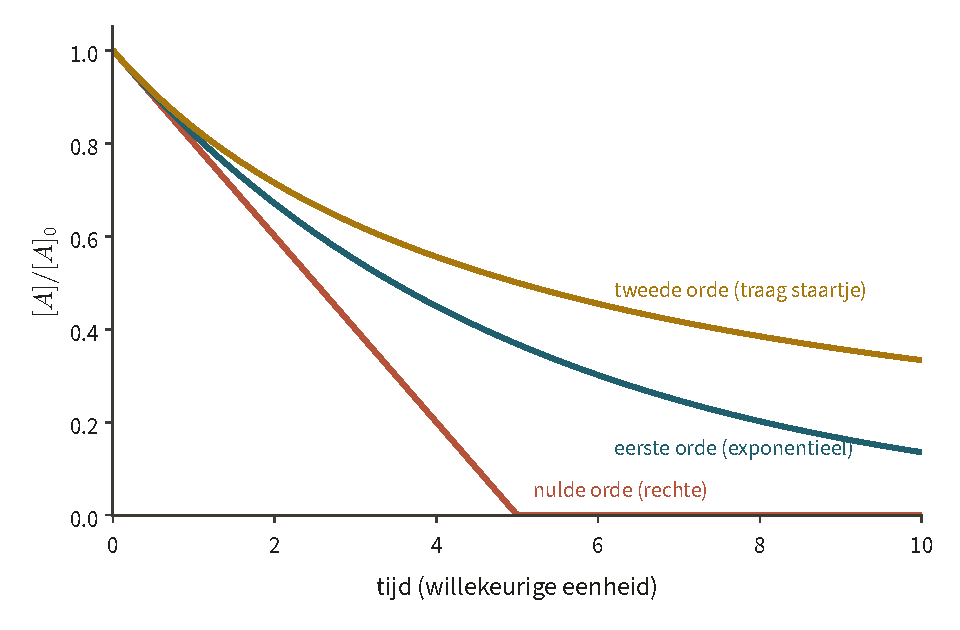
\includegraphics[width=0.7\linewidth]{Figuren/ordes}
    \caption{Concentratieverloop voor een nulde-, eerste- en tweede-orde reactie met dezelfde beginconcentratie en dezelfde beginsnelheid. Een rechte (nulde orde), een exponenti\"ele daling (eerste orde) en een trage staart (tweede orde): de integratiemethode maakt van dit verschil gebruik.}
    \label{fig:ordes-concentratie-tijd}
\end{figure}

\subsection{Bepaling van de reactieorde}
\label{sec:bepaling-orde}

De reactieorde kan experimenteel worden bepaald door:
\begin{itemize}
\item \textbf{De integratiemethode}: test of $\ln[A]$, $1/[A]$ of $[A]$ lineair verloopt met de tijd (figuur~\ref{fig:ordes-concentratie-tijd}).
\item \textbf{De isolatiemethode}: houd alle reactanten behalve \'e\'en in groot overschot, zodat hun concentratie constant is. De reactieorde met betrekking tot de vari\"erende component wordt zo ge\"isoleerd.
\item \textbf{De methode van initi\"ele snelheden}: meet $r$ aanvankelijk voor verschillende beginconcentraties en vergelijk $\log r$ met $\log[A]$.
\end{itemize}

\section{De invloed van temperatuur: de vergelijking van Arrhenius}
\label{sec:arrhenius}

Voor nagenoeg alle chemische reacties neemt de reactiesnelheid sterk toe met de temperatuur. Een ruwe vuistregel: per \SI{10}{\kelvin} verdubbelt de snelheid. Kwantitatief geldt de \emph{vergelijking van Arrhenius}:
\begin{equation}
\boxed{\;k = A\,\exp\!\left(-\frac{E_a}{RT}\right)\;}
\label{eq:arrhenius}
\end{equation}
met $A$ de \emph{pre\"exponenti\"ele factor} en $E_a$ de \emph{activeringsenergie}, de energiedrempel tussen reagentia en overgangstoestand (\S~\ref{sec:activeringsenergie-kwantum}). De exponenti\"ele vorm verklaart waarom de snelheid zo sterk met de temperatuur stijgt: een verhoging van $T$ verhoogt de fractie van de moleculen met voldoende energie om de activeringsdrempel te overschrijden. Merk meteen op dat deze fractie, en dus de \emph{gevoeligheid} van $k$ voor temperatuur, sterker is naarmate $E_a$ groter is --- een inzicht dat we in \S~\ref{sec:temperatuursgevoeligheid} kwantitatief zullen uitwerken.

\subsection{De betekenis van de activeringsenergie}

De activeringsenergie $E_a$ is de minimale energie die een molecule (of een paar botsende moleculen) moet bezitten om de reactie te laten plaatsvinden. Uit de vergelijking van Arrhenius volgt:
\begin{equation}
\ln k = \ln A - \frac{E_a}{RT}.
\label{eq:arrhenius-log}
\end{equation}
Door $\ln k$ uit te zetten tegen $1/T$ ontstaat een rechte met helling $-E_a/R$. Dit is de \emph{Arrhenius-grafiek}, waarmee $E_a$ uit experimentele snelheidsmetingen bij verschillende temperaturen kan worden bepaald.

\begin{figure}[htb]
    \centering
    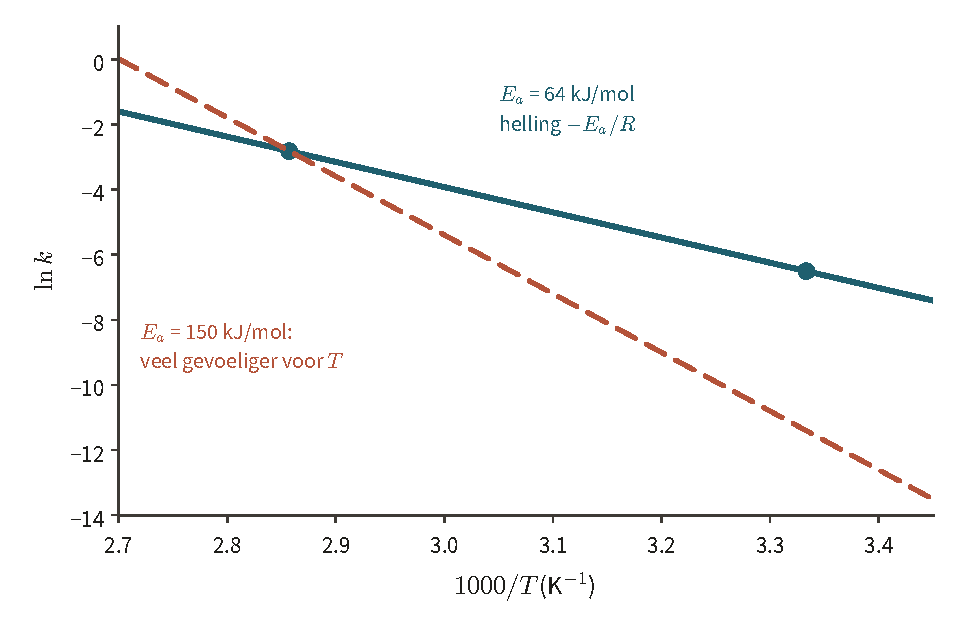
\includegraphics[width=0.7\linewidth]{Figuren/arrhenius}
    \caption{Arrheniusgrafiek: $\ln k$ tegen $1/T$ geeft een rechte met helling $-E_a/R$. De punten zijn de twee metingen uit het voorbeeld hieronder. De stippellijn is een reactie met een hogere activeringsenergie: ze is veel gevoeliger voor de temperatuur.}
    \label{fig:arrhenius-grafiek}
\end{figure}

\begin{voorbeeld}{Bepaling van $E_a$ uit twee metingen}
Voor een bepaalde reactie is $k = \SI{1.5e-3}{\per\second}$ bij \SI{300}{\kelvin} en $k = \SI{6.0e-2}{\per\second}$ bij \SI{350}{\kelvin}. Uit de ge\"integreerde Arrheniusvergelijking (volledig analoog aan de ge\"integreerde vergelijking van Van 't Hoff, hoofdstuk~\ref{ch:reagerend}):
\[
\ln\frac{k_2}{k_1} = -\frac{E_a}{R}\left(\frac{1}{T_2} - \frac{1}{T_1}\right)
\]
volgt:
\[
E_a = -R\,\frac{\ln(k_2/k_1)}{(1/T_2 - 1/T_1)} = -(\SI{8.314}{\joule\per\mole\per\kelvin})\frac{\ln(40)}{1/350 - 1/300} \approx \SI{64.4}{\kilo\joule\per\mole}.
\]
Een activeringsenergie van \SI{64}{\kilo\joule\per\mole} is typisch voor vele thermisch geactiveerde reacties.
\end{voorbeeld}

\interactief{arrhenius}

\subsection{Temperatuurverhoging bij ammoniaksynthese}
\label{sec:ammoniak-arrhenius}

Voor de ammoniaksynthese geldt $E_a \approx \SI{230}{\kilo\joule\per\mole}$ (zeer hoog wegens de sterke drievoudige stikstofbinding, hoofdstuk~\ref{ch:kwantum}). Een verhoging van \SI{300}{\kelvin} naar \SI{700}{\kelvin} levert:
\[
\frac{k(700)}{k(300)} = \exp\left[-\frac{230\,000}{8.314}\left(\frac{1}{700} - \frac{1}{300}\right)\right] \approx 7.7\times10^{22}.
\]
De reactiesnelheid neemt astronomisch toe. Dit verklaart waarom het Haber--Boschproces ondanks de thermodynamisch ongunstige hoge temperatuur toch bij \SIrange{400}{500}{\celsius} wordt uitgevoerd (hoofdstuk~\ref{ch:reagerend}, \S~\ref{sec:haber-bosch-integraal}): zonder voldoende temperatuur zou de kinetiek het proces volledig onmogelijk maken, ondanks de thermodynamische gunst bij lage temperatuur. We komen op dit precieze getal terug in \S~\ref{sec:temperatuursgevoeligheid}, waar we het vergelijken met de temperatuursgevoeligheid van de \emph{teruggaande} reactie.

\section{Waarom Arrhenius? De botsingstheorie}
\label{sec:botsingstheorie}

De vergelijking van Arrhenius is empirisch. Voor gasreacties kunnen we haar begrijpen met de kinetische gastheorie van hoofdstuk~\ref{ch:energie} (\S~\ref{sec:kinetische-gastheorie}): twee moleculen kunnen pas reageren als ze botsen, en enkel als die botsing hard genoeg is.

\subsection{Snelheden, botsingen en vrije weglengte}

De moleculen in een gas hebben niet allemaal dezelfde snelheid. De verdeling volgt uit de Boltzmannfactor (hoofdstuk~\ref{ch:kwantum}, \S~\ref{sec:boltzmannverdeling}) toegepast op de kinetische energie $\tfrac12 mv^2$; ze heet de \emph{Maxwell--Boltzmannverdeling}:
\begin{equation}
f(v) = 4\pi\left(\frac{M}{2\pi RT}\right)^{3/2} v^2\,\exp\!\left(-\frac{Mv^2}{2RT}\right),
\qquad
\bar v = \sqrt{\frac{8RT}{\pi M}}.
\label{eq:maxwell-boltzmann}
\end{equation}
De factor $v^2$ telt het aantal richtingen waarin een molecule met snelheid $v$ kan bewegen; de exponenti\"ele factor maakt hoge snelheden zeldzaam. Bij hogere temperatuur schuift de verdeling op en wordt ze breder (figuur~\ref{fig:maxwell-boltzmann}). Vooral de staart met zeer snelle moleculen groeit sterk: daar zitten de moleculen die kunnen reageren.

\begin{figure}[htb]
    \centering
    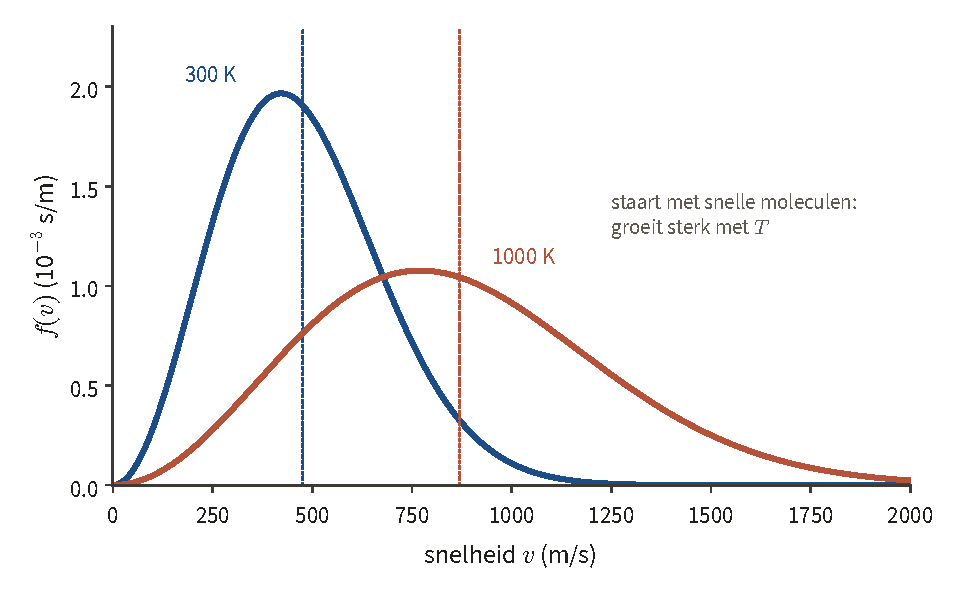
\includegraphics[width=0.7\linewidth]{Figuren/maxwell_boltzmann}
    \caption{Maxwell--Boltzmannverdeling van de snelheid van N$_2$ bij \SI{300}{\kelvin} en \SI{1000}{\kelvin}. De stippellijnen geven de gemiddelde snelheid $\bar v$.}
    \label{fig:maxwell-boltzmann}
\end{figure}

Een molecule met diameter $d$ botst met elk ander molecule waarvan het centrum binnen een cilinder met doorsnede $\sigma = \pi d^2$ (de \emph{botsingsdoorsnede}) ligt. Daaruit volgen de \emph{botsingsfrequentie} van \'e\'en molecule en de gemiddelde afstand tussen twee botsingen, de \emph{vrije weglengte}:
\begin{equation}
z = \sqrt2\,\sigma\,\bar v\,\frac{p}{k_BT},
\qquad
\lambda = \frac{\bar v}{z} = \frac{k_BT}{\sqrt2\,\sigma\,p}.
\label{eq:vrije-weglengte}
\end{equation}
De factor $\sqrt2$ komt van de relatieve snelheid tussen twee bewegende moleculen.

\begin{voorbeeld}{Stikstof bij kamertemperatuur}
Voor N$_2$ bij \SI{298}{\kelvin} en \SI{1}{\bar} is $\sigma \approx \SI{0.43}{\nano\metre\squared}$ en $\bar v = \sqrt{8(8.314)(298)/(\pi\cdot0.028)} = \SI{475}{\metre\per\second}$. Dan is
\[
\lambda = \frac{(\SI{1.381e-23}{})(298)}{\sqrt2\,(\SI{0.43e-18}{})(\SI{1e5}{})} = \SI{68}{\nano\metre},
\qquad
z = \frac{\bar v}{\lambda} = \SI{7e9}{\per\second}.
\]
Elke molecule botst zeven miljard keer per seconde, en legt tussen twee botsingen een afstand af van ongeveer tweehonderd keer haar eigen diameter.
\end{voorbeeld}

\begin{toepassing}{Vacuüm, poriën en isotopen: drie praktische haakjes}
\begin{itemize}
\item \textbf{Vacuümtechniek.} De vrije weglengte is omgekeerd evenredig met de druk. Bij \SI{e-6}{\milli\bar} (\SI{e-4}{\pascal}), typisch voor een coatingkamer of elektronenmicroscoop, is $\lambda \approx \SI{70}{\metre}$: moleculen botsen enkel nog tegen de wanden. Men spreekt van \emph{moleculaire stroming}, en de pompsnelheid wordt dan bepaald door de opening en niet meer door de viscositeit van het gas.
\item \textbf{Knudsendiffusie.} Is de vrije weglengte groter dan de poriediameter $d_p$ (het \emph{Knudsengetal} $\mathrm{Kn} = \lambda/d_p > 1$), dan botsen moleculen vaker met de wand dan met elkaar. In de poriën van \SI{10}{\nano\metre} van de katalysatorkorrel uit hoofdstuk~\ref{ch:grensvlakken} is dat al zo bij \SI{1}{\bar}. De diffusieco\"effici\"ent hangt dan af van $\bar v$ en de poriegrootte, niet van de druk.
\item \textbf{Effusie.} Door een gaatje dat kleiner is dan $\lambda$ ontsnappen moleculen met een snelheid evenredig met $\bar v \propto 1/\sqrt{M}$: de wet van Graham uit hoofdstuk~\ref{ch:energie}.
\end{itemize}
\end{toepassing}

\subsection{Van botsing naar reactie}

Niet elke botsing leidt tot een reactie. Twee voorwaarden moeten vervuld zijn:
\begin{enumerate}
\item De botsing moet genoeg energie hebben: de kinetische energie langs de verbindingslijn van beide centra moet minstens $E_a$ zijn. De fractie botsingen die daaraan voldoet, is precies de Boltzmannfactor $\exp(-E_a/RT)$.
\item De moleculen moeten juist gericht zijn. Bij grote moleculen leidt enkel een klein deel van de botsingen tot reactie. Dat deel heet de \emph{sterische factor} $P$.
\end{enumerate}
Het aantal botsingen per volume en per tijd tussen A en B is $\sigma\,\bar v_\mathrm{rel}\,N_A^2[A][B]$, met $\bar v_\mathrm{rel} = \sqrt{8RT/\pi\mu}$ en $\mu$ de gereduceerde molaire massa. Vermenigvuldigen met beide fracties geeft de snelheidsconstante:
\begin{equation}
\boxed{\;k = P\,\sigma\,\bar v_\mathrm{rel}\,N_A\,\exp\!\left(-\frac{E_a}{RT}\right)\;}
\label{eq:botsingstheorie}
\end{equation}
Dat is de vergelijking van Arrhenius, met een pre\"exponenti\"ele factor $A = P\,\sigma\,\bar v_\mathrm{rel}\,N_A$. De exponenti\"ele factor bevat bijna alle temperatuursafhankelijkheid; $A$ stijgt slechts met $\sqrt T$.

\begin{voorbeeld}{Hoe groot kan $A$ zijn?}
Voor twee moleculen zo groot als N$_2$ ($\sigma = \SI{0.43}{\nano\metre\squared}$, $\bar v_\mathrm{rel} = \sqrt2\cdot\SI{475}{\metre\per\second} = \SI{672}{\metre\per\second}$) bij kamertemperatuur:
\begin{align*}
A = \sigma\,\bar v_\mathrm{rel}\,N_A &= (\SI{0.43e-18}{\metre\squared})(\SI{672}{\metre\per\second})(\SI{6.022e23}{\per\mole})\\
&= \SI{1.7e8}{\metre\cubed\per\mole\per\second} = \SI{1.7e11}{\litre\per\mole\per\second}.
\end{align*}
Gemeten waarden voor eenvoudige radicaalreacties liggen in die buurt ($P \approx 0.1$--1). Voor reacties tussen grote organische moleculen meet men vaak $10^{-3}$ tot $10^{-6}$ keer minder: de sterische factor is dan klein, omdat slechts een klein stukje van elk molecule reactief is.
\end{voorbeeld}

De botsingstheorie verklaart dus waarom $\ln k$ lineair daalt met $1/T$, en waarom een hogere activeringsenergie een sterkere temperatuursafhankelijkheid geeft. Voor reacties in oplossing en op oppervlakken is het beeld minder eenvoudig, maar de Boltzmannfactor blijft de kern.

\section{Omkeerbare en concurrerende reacties}
\label{sec:meervoudige-reacties}

Industri\"ele reacties verlopen zelden alleen. Het product kan terugreageren, de grondstof kan op meer dan \'e\'en manier reageren, en het gewenste product kan zelf verder reageren. Voor de ingenieur is niet alleen de \emph{omzetting} $X$ belangrijk, maar vooral de \emph{selectiviteit} $S$ (welk deel van de omgezette grondstof wordt gewenst product) en de \emph{opbrengst} $Y = X\,S$.

\subsection{Omkeerbare reacties: de weg naar evenwicht}
\label{sec:omkeerbare-reacties}

Voor $A \rightleftharpoons B$ met eerste-orde snelheidsconstanten $k_1$ (heen) en $k_{-1}$ (terug) geldt
\[
-\frac{\dd{[A]}}{\dd{t}} = k_1[A] - k_{-1}[B].
\]
In evenwicht is de netto snelheid nul: $K = [B]_\mathrm{eq}/[A]_\mathrm{eq} = k_1/k_{-1}$. Dit is dezelfde $K$ als in hoofdstuk~\ref{ch:reagerend}. Integratie geeft
\begin{equation}
[A] - [A]_\mathrm{eq} = \bigl([A]_0 - [A]_\mathrm{eq}\bigr)\,e^{-(k_1+k_{-1})t}.
\label{eq:relaxatie}
\end{equation}
Het systeem nadert het evenwicht exponentieel, met een karakteristieke tijd $1/(k_1+k_{-1})$: de \emph{som} van beide snelheidsconstanten, niet $k_1$ alleen. De thermodynamica (via $K$) zegt waar de reactie eindigt; de kinetiek zegt hoe snel. In \S~\ref{sec:brug-thermo-kinetiek} volgt hieruit een verband tussen de activeringsenergie\"en en $\Delta_rH^\circ$.

\subsection{Parallelle reacties en selectiviteit}
\label{sec:selectiviteit}

Bij twee \emph{parallelle} reacties uit dezelfde grondstof,
\[
A \xrightarrow{k_1} B \ \text{(gewenst)}, \qquad A \xrightarrow{k_2} C \ \text{(ongewenst)},
\]
met dezelfde orde in $A$, is de verhouding van de vormingssnelheden constant, en de selectiviteit
\begin{equation}
S = \frac{k_1}{k_1 + k_2} = \frac{1}{1 + \dfrac{A_2}{A_1}\exp\!\left(-\dfrac{E_{a,2} - E_{a,1}}{RT}\right)}.
\label{eq:selectiviteit}
\end{equation}
De temperatuur werkt dus in het voordeel van de reactie met de \emph{hoogste} activeringsenergie. Twee regels volgen meteen:
\begin{itemize}
\item Heeft de gewenste reactie de laagste $E_a$, dan geeft een lage temperatuur een betere selectiviteit, maar een tragere reactie. Een selectieve katalysator verlaagt vooral $E_{a,1}$.
\item Verschillen de reactieordes, dan speelt ook de concentratie mee: is de gewenste reactie van hogere orde in $A$, dan houdt men $[A]$ hoog (batch- of propstroomreactor); is ze van lagere orde, dan werkt men verdund (geroerde tank, CSTR).
\end{itemize}

\begin{voorbeeld}{Ethyleenoxide: selectiviteit en temperatuur}
Neem voor de centrale case $E_{a,1} \approx \SI{60}{\kilo\joule\per\mole}$ voor de epoxidering en $E_{a,2} \approx \SI{80}{\kilo\joule\per\mole}$ voor de volledige verbranding (illustratieve waarden), en kies $A_2/A_1$ zo dat $S = 0.85$ bij \SI{500}{\kelvin}. Met vergelijking~\eqref{eq:selectiviteit}:
\begin{center}
\begin{tabular}{lccc}
\toprule
$T$ (K) & 470 & 500 & 550 \\
\midrule
$S$ & 0.885 & 0.85 & 0.79 \\
warmte per mol omgezet ethyleen (kJ) & 245 & 288 & 366 \\
\bottomrule
\end{tabular}
\end{center}
De warmte is $S(105) + (1-S)(1323)$~kJ. Vijftig graden warmer kost zes procentpunten selectiviteit en levert een kwart meer warmte. Die extra warmte maakt de reactor nog warmer, wat de selectiviteit verder verlaagt: een gevaarlijke terugkoppeling (\S~\ref{sec:runaway}). Daarom bewaakt men de temperatuur van een EO-reactor tot op enkele graden en voegt men kleine hoeveelheden gechloreerde moderatoren toe die de verbranding sterker afremmen dan de epoxidering.
\end{voorbeeld}

\subsection{Reacties in serie: het tussenproduct}
\label{sec:serie-reacties}

Vaak is het gewenste product zelf reactief: $A \xrightarrow{k_1} B \xrightarrow{k_2} C$. Denk aan de gedeeltelijke oxidatie van koolwaterstoffen, waar het product verder verbrandt, of aan een geneesmiddel dat in het lichaam wordt omgezet tot een actieve vorm en daarna afgebroken. Met eerste-orde kinetiek en enkel $A$ bij de start volgt
\begin{equation}
[A] = [A]_0\,e^{-k_1t},
\qquad
[B] = [A]_0\,\frac{k_1}{k_2-k_1}\bigl(e^{-k_1t} - e^{-k_2t}\bigr).
\label{eq:serie}
\end{equation}
Het tussenproduct stijgt eerst, bereikt een maximum en verdwijnt dan (figuur~\ref{fig:serie-reactie}). Afleiden van $[B]$ naar $t$ en gelijkstellen aan nul geeft het optimum:
\begin{equation}
\boxed{\;t_\mathrm{max} = \frac{\ln(k_2/k_1)}{k_2-k_1},
\qquad
\frac{[B]_\mathrm{max}}{[A]_0} = \left(\frac{k_1}{k_2}\right)^{k_2/(k_2-k_1)}\;}
\label{eq:serie-max}
\end{equation}

\begin{figure}[htb]
    \centering
    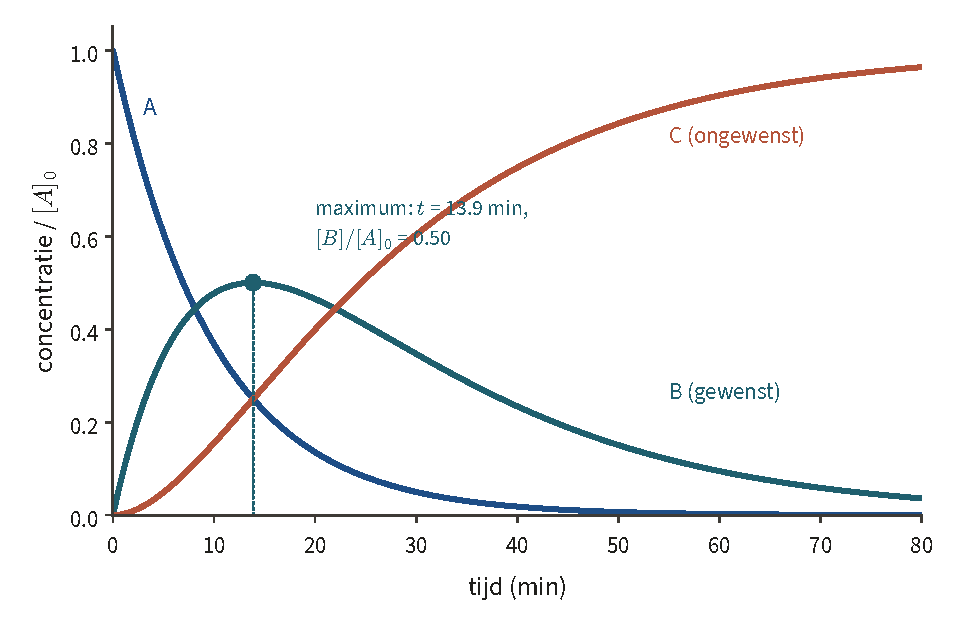
\includegraphics[width=0.7\linewidth]{Figuren/serie_reactie}
    \caption{Reacties in serie $A \to B \to C$ met $k_1 = \SI{0.10}{\per\minute}$ en $k_2 = \SI{0.05}{\per\minute}$. Het tussenproduct $B$ bereikt een maximum; wie te lang wacht, verliest het gewenste product.}
    \label{fig:serie-reactie}
\end{figure}

Voor $k_1 = \SI{0.10}{\per\minute}$ en $k_2 = \SI{0.05}{\per\minute}$ is $t_\mathrm{max} = \ln 0.5/(-0.05) = \SI{13.9}{\minute}$ en $[B]_\mathrm{max} = 0.50\,[A]_0$. De les voor de ingenieur: bij reacties in serie is maximale omzetting \emph{niet} het doel. Men stopt de batch op het juiste moment, of kiest in een continue reactor de verblijftijd zo dat de opbrengst aan $B$ maximaal is, en recycleert de niet-omgezette $A$.

\section{Reactiemechanismen en elementaire reacties}
\label{sec:mechanismen}

Bijna geen enkele reactie verloopt in \'e\'en stap. De brutoreactie beschrijft enkel begin- en eindtoestand; de weg ertussen is het \emph{reactiemechanisme}, een reeks \emph{elementaire reacties}. Een elementaire reactie is \'e\'en moleculaire gebeurtenis: een molecule die uiteenvalt (\emph{unimoleculair}), twee moleculen die botsen (\emph{bimoleculair}) of, zelden, drie tegelijk (\emph{termoleculair}). Alleen voor elementaire reacties volgt de orde uit de stoichiometrie: $A + B \rightarrow P$ is dan altijd $r = k[A][B]$.

Een klassiek voorbeeld is $\mathrm{H_2 + Br_2 \rightarrow 2\,HBr}$. De reactie verloopt via een radicaalketen:
\begin{align*}
&\text{initiatie:} && \mathrm{Br_2} \rightarrow 2\,\mathrm{Br\cdot}\\
&\text{propagatie:} && \mathrm{Br\cdot + H_2} \rightarrow \mathrm{HBr + H\cdot}, \qquad \mathrm{H\cdot + Br_2} \rightarrow \mathrm{HBr + Br\cdot}\\
&\text{terminatie:} && 2\,\mathrm{Br\cdot} \rightarrow \mathrm{Br_2}
\end{align*}
met als gemeten snelheidswet $r = k[\mathrm{H_2}][\mathrm{Br_2}]^{1/2}/(1 + k'[\mathrm{HBr}]/[\mathrm{Br_2}])$. Die vorm volgt nooit uit de brutovergelijking; je hebt het mechanisme nodig.

\section{De steady-state-benadering}
\label{sec:steady-state}

Reactieve tussenproducten (radicalen, een enzym-substraatcomplex, een geactiveerde molecule) worden even snel verbruikt als gevormd. Hun concentratie blijft klein en nagenoeg constant. De \emph{steady-state-benadering} (Bodenstein) stelt daarom
\begin{equation}
\frac{\dd{[\text{tussenproduct}]}}{\dd{t}} \approx 0 .
\end{equation}
Is \'e\'en stap veel trager dan de rest, dan bepaalt die \emph{snelheidsbepalende stap} de globale snelheid, zoals de smalste flessenhals de doorstroming bepaalt.

\subsection{Voorbeeld: ontleding van ozon}
\label{sec:ozon}

$\mathrm{2\,O_3 \rightarrow 3\,O_2}$ verloopt via een snel evenwicht $\mathrm{O_3} \rightleftharpoons \mathrm{O_2 + O}$ ($k_1$, $k_{-1}$) en een trage stap $\mathrm{O + O_3} \rightarrow 2\,\mathrm{O_2}$ ($k_2$). Steady state voor het zuurstofatoom:
\[
k_1[\mathrm{O_3}] - k_{-1}[\mathrm{O_2}][\mathrm{O}] - k_2[\mathrm{O}][\mathrm{O_3}] = 0 .
\]
Omdat de tweede stap traag is ($k_2[\mathrm{O_3}] \ll k_{-1}[\mathrm{O_2}]$), volgt
\[
[\mathrm{O}] \approx \frac{k_1[\mathrm{O_3}]}{k_{-1}[\mathrm{O_2}]},
\qquad
r = k_2[\mathrm{O}][\mathrm{O_3}] = \frac{k_1 k_2}{k_{-1}} \frac{[\mathrm{O_3}]^2}{[\mathrm{O_2}]}.
\]
Het product \ce{O2} remt de reactie: iets wat je uit de brutovergelijking nooit zou raden.

\subsection{Het Lindemann-mechanisme}
\label{sec:lindemann}

Een molecule die ``gewoon uit elkaar valt'' ($A \to P$), gedraagt zich bij hoge druk als eerste orde, maar bij lage druk als tweede orde. Lindemann (1922) verklaarde dat: de molecule moet eerst energie krijgen door een botsing, en kan die bij een volgende botsing weer verliezen:
\[
A + A \xrightleftharpoons[k_{-1}]{k_1} A^* + A, \qquad A^* \xrightarrow{k_2} P .
\]
Steady state voor $A^*$ geeft $[A^*] = k_1[A]^2/(k_{-1}[A]+k_2)$, en met $r = k_2[A^*]$:
\begin{equation}
\boxed{\;r = \frac{k_1k_2[A]^2}{k_{-1}[A]+k_2}\;}
\label{eq:lindemann}
\end{equation}
Bij \textbf{hoge druk} ($k_{-1}[A] \gg k_2$) wordt een geactiveerde molecule meestal eerst weer gedeactiveerd: $r \approx (k_1k_2/k_{-1})[A]$, eerste orde. Bij \textbf{lage druk} ($k_2 \gg k_{-1}[A]$) reageert elke geactiveerde molecule meteen: $r \approx k_1[A]^2$, tweede orde, want de activerende botsing is nu de flessenhals (figuur~\ref{fig:lindemann}).

\begin{figure}[htb]
    \centering
    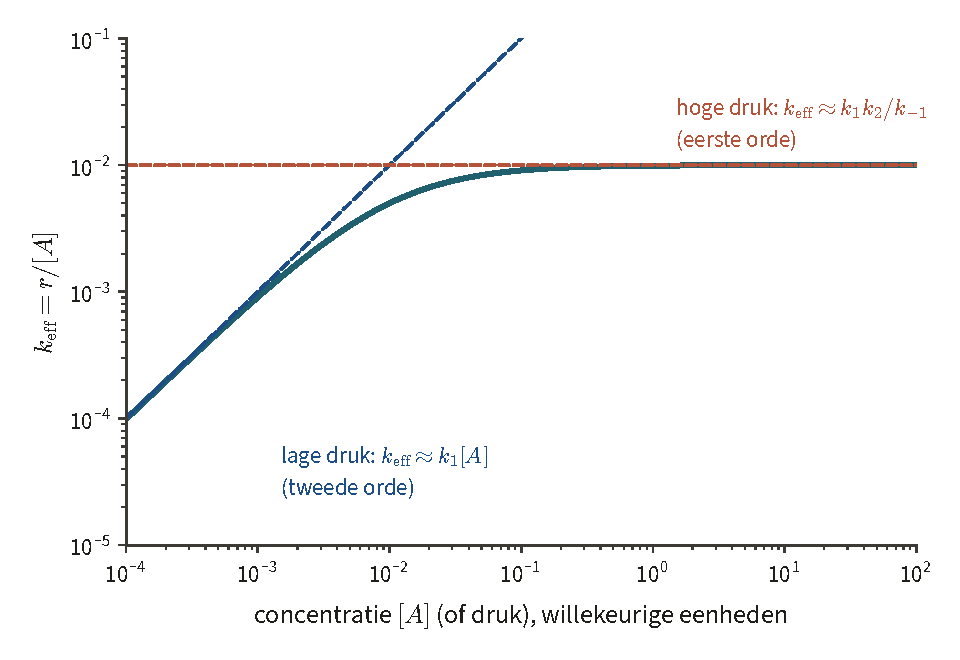
\includegraphics[width=0.7\linewidth]{Figuren/lindemann}
    \caption{Lindemann-mechanisme: de effectieve eerste-ordeconstante $k_\text{eff} = r/[A]$ in functie van de concentratie (logaritmische assen). Bij lage druk stijgt $k_\text{eff}$ evenredig met $[A]$ (tweede orde), bij hoge druk vlakt ze af tot $k_1k_2/k_{-1}$ (eerste orde). Michaelis--Menten en Langmuir--Hinshelwood tonen dezelfde verzadiging.}
    \label{fig:lindemann}
\end{figure}

Dit patroon (een orde die verschuift doordat een tussenstap verzadigt) komt verderop nog twee keer terug: bij enzymen (\S~\ref{sec:michaelis-menten}) en bij katalysatoroppervlakken (\S~\ref{sec:langmuir-hinshelwood}).

\section{Katalyse}
\label{sec:katalyse}

Een \emph{katalysator} verhoogt de reactiesnelheid zonder zelf verbruikt te worden. Hij verlaagt de activeringsenergie van heen- \'en terugreactie evenveel, zodat de evenwichtsconstante niet verandert (hoofdstuk~\ref{ch:reagerend}).

\subsection{Het principe}
\label{sec:katalyse-principe}

De katalysator biedt een andere weg met een lagere barri\`ere (figuur~\ref{fig:reactiecoordinaat-katalysator}). Volgens Arrhenius is de versnelling
\begin{equation}
\boxed{\;\frac{k_{\text{kat}}}{k_{\text{onkat}}} = \frac{A_{\text{kat}}}{A_{\text{onkat}}}\,\exp\!\left(\frac{E_{a,\text{onkat}} - E_{a,\text{kat}}}{RT}\right)\;}
\label{eq:katalysator-versnelling}
\end{equation}
Een verlaging van $E_a$ van \SI{150}{\kilo\joule\per\mole} naar \SI{75}{\kilo\joule\per\mole} geeft bij \SI{298}{\kelvin} (gelijke $A$) een factor $\exp(75\,000/(8.314 \cdot 298)) = e^{30.3} \approx 10^{13}$.

\begin{figure}[htb]
    \centering
    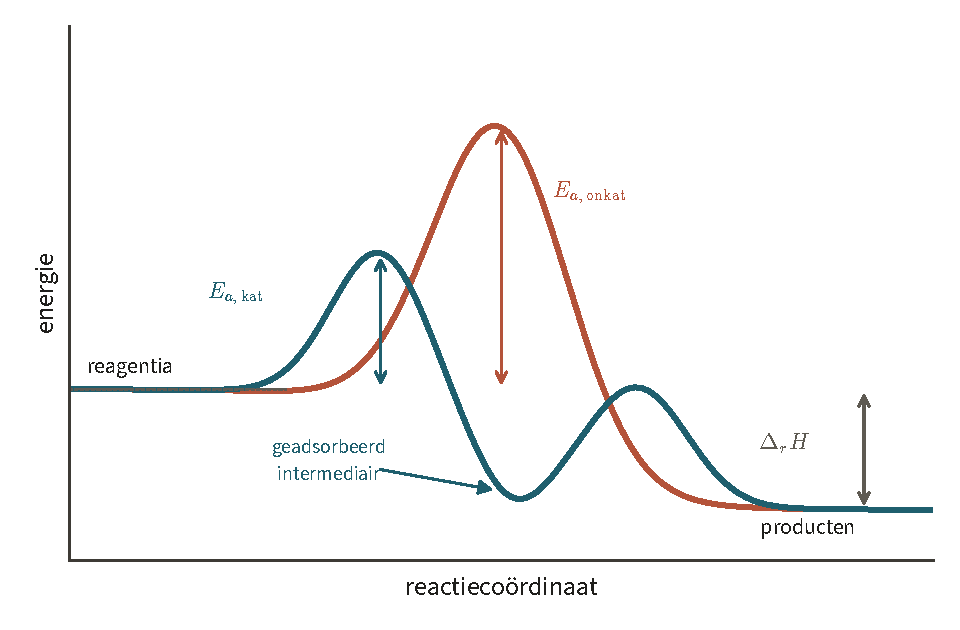
\includegraphics[width=0.7\linewidth]{Figuren/reactiecoordinaat}
    \caption{Energieprofiel met en zonder katalysator. De katalysator biedt een andere weg met lagere barri\`eres, vaak via een geadsorbeerd intermediair. Begin- en eindtoestand blijven dezelfde: $\Delta_rH$ en de evenwichtsligging veranderen niet.}
    \label{fig:reactiecoordinaat-katalysator}
\end{figure}

\subsection{Homogeen versus heterogeen}
\label{sec:homogeen-heterogeen}

Het belangrijkste onderscheid voor de ingenieur is de fase (tabel~\ref{tab:homogeen-heterogeen}). Homogene katalysatoren zijn vaak selectiever en via hun liganden fijn af te stemmen, maar het product moet er nadien van gescheiden worden. Een vast katalysatorbed scheidt zichzelf. Daarom zijn de grote processen (Haber--Bosch, het contactproces, katalytisch kraken) bijna allemaal heterogeen.

\begin{table}[htb]
\centering
\caption{Homogene en heterogene katalyse vergeleken.}
\label{tab:homogeen-heterogeen}
\begin{tabular}{lll}
\toprule
 & Homogeen & Heterogeen \\
\midrule
Fase katalysator & zelfde fase als reactanten & andere fase (meestal vast) \\
Actieve plaatsen & elke molecule & enkel oppervlakteatomen \\
Selectiviteit & doorgaans hoog, afstembaar & vaak lager, wel robuust \\
Productscheiding & moeilijk (destillatie) & eenvoudig (vast bed) \\
Thermische stabiliteit & beperkt & doorgaans hoog \\
Voorbeelden & zuur/base, Rh-complex, enzym & Fe, \ce{V2O5}, Pt, zeoliet \\
\bottomrule
\end{tabular}
\end{table}

\subsection{Homogene katalyse}
\label{sec:homogene-katalyse}

Typische homogene katalysatoren zijn zuren en basen (esterhydrolyse, inversie van sucrose), opgeloste metaalcomplexen (de Wilkinsonkatalysator \ce{RhCl(PPh3)3} voor hydrogenering, Pd voor koppelingsreacties) en enzymen. Het \emph{Monsanto-proces} zet methanol en CO om tot azijnzuur met een opgelost rhodiumcomplex bij \SIrange{150}{200}{\celsius} en \SIrange{30}{60}{\bar}, met een selectiviteit boven \SI{99}{\percent}.

\subsection{Heterogene katalyse}
\label{sec:heterogene-katalyse}

Een reactie op een vaste katalysator doorloopt vijf stappen (figuur~\ref{fig:katalyse-stappen}): (1) diffusie naar het oppervlak, (2) adsorptie, (3) reactie aan het oppervlak, (4) desorptie, (5) diffusie terug naar de gasfase. De traagste stap bepaalt de snelheid.

\begin{figure}[htb]
    \centering
    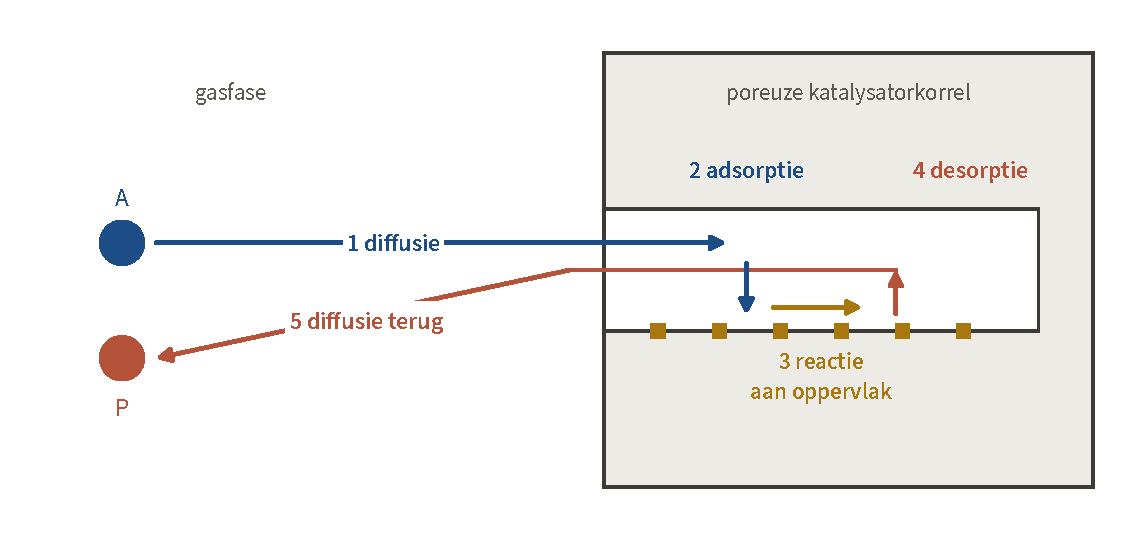
\includegraphics[width=0.85\linewidth]{Figuren/katalyse_stappen}
    \caption{De vijf stappen van een heterogeen gekatalyseerde reactie in een poreuze katalysatorkorrel. Stappen 1 en 5 zijn transport, stappen 2 tot 4 oppervlaktechemie.}
    \label{fig:katalyse-stappen}
\end{figure}

\subsubsection{Diffusie: stappen 1 en 5}
\label{sec:diffusie-katalyse}

Diffusie volgt de \emph{eerste wet van Fick}: de flux is evenredig met de concentratiegradi\"ent,
\begin{equation}
\boxed{\;j = -D\,\frac{\dd{c}}{\dd{x}}\;}
\label{eq:fick}
\end{equation}
met $D$ de diffusieco\"effici\"ent (\si{\metre\squared\per\second}). Daaruit volgt de belangrijkste vuistregel van transport: de tijd om een afstand $L$ te overbruggen, schaalt met het \emph{kwadraat} van die afstand,
\begin{equation}
\boxed{\;t_{\text{diff}} \approx \frac{L^2}{D}\;}
\label{eq:diffusietijdschaal}
\end{equation}

\begin{voorbeeld}{Diffusietijd in een poreuze katalysatorkorrel}
Met $D \approx \SI{1e-5}{\metre\squared\per\second}$ (gas in poriën) is $t_\text{diff} \approx \SI{0.1}{\second}$ voor een korrel met straal \SI{1}{\milli\metre}, maar slechts \SI{10}{\micro\second} voor \SI{10}{\micro\metre}. Honderd keer kleiner is tienduizend keer sneller. Kleine korrels houden de oppervlaktereactie snelheidsbepalend, maar geven een grotere drukval over het bed: een klassieke ontwerpafweging voor Reactorentechnologie.
\end{voorbeeld}

\subsubsection{Adsorptie en Langmuir--Hinshelwood-kinetiek}
\label{sec:adsorptie-kinetiek}
\label{sec:langmuir-hinshelwood}

Adsorptie (fysisorptie en chemisorptie, de Langmuir-isotherme, BET) kwam aan bod in hoofdstuk~\ref{ch:grensvlakken} (\S~\ref{sec:fysisorptie-chemisorptie} tot \S~\ref{sec:bet}). Chemisorptie verzwakt de bindingen van het reagens en verlaagt zo de barri\`ere van de oppervlaktereactie. Moeten \emph{beide} reactanten adsorberen en is de oppervlaktereactie snelheidsbepalend, dan is $r = k\,\theta_A\theta_B$. Met de competitieve Langmuir-isotherme (vergelijking~\eqref{eq:langmuir-competitief}) volgt de \emph{Langmuir--Hinshelwood}-snelheidswet:
\begin{equation}
r = \frac{k\,K_A\,K_B\,p_A\,p_B}{(1 + K_A\,p_A + K_B\,p_B)^2}.
\label{eq:langmuir-hinshelwood}
\end{equation}
Bij lage druk is het oppervlak bijna leeg en $r \approx kK_AK_Bp_Ap_B$. Bij hoge $p_A$ verdringt $A$ het andere reagens van het oppervlak, en de snelheid \emph{daalt} weer (figuur~\ref{fig:lh-vs-er}). Zo werkt CO-oxidatie op platina, en zo werkt ook de ammoniaksynthese op ijzer.

\subsubsection{Eley--Rideal-kinetiek}
\label{sec:eley-rideal}
\label{sec:lh-vs-er-onderscheid}

Bij het \emph{Eley--Rideal}-mechanisme adsorbeert enkel $A$, en $B$ reageert er rechtstreeks vanuit de gasfase mee:
\begin{equation}
r = k\,\theta_A\,p_B = \frac{k\,K_A\,p_A\,p_B}{1+K_A\,p_A}.
\label{eq:eley-rideal}
\end{equation}
Bij lage $p_A$ geven beide mechanismen hetzelfde. Bij hoge $p_A$ verschillen ze: Langmuir--Hinshelwood heeft een maximum, Eley--Rideal stijgt naar een plateau, want een volledig met $A$ bedekt oppervlak is voor $B$ juist ideaal. Dat verschil in het hogedrukgedrag is het experimentele criterium om beide te onderscheiden.

\begin{figure}[htb]
    \centering
    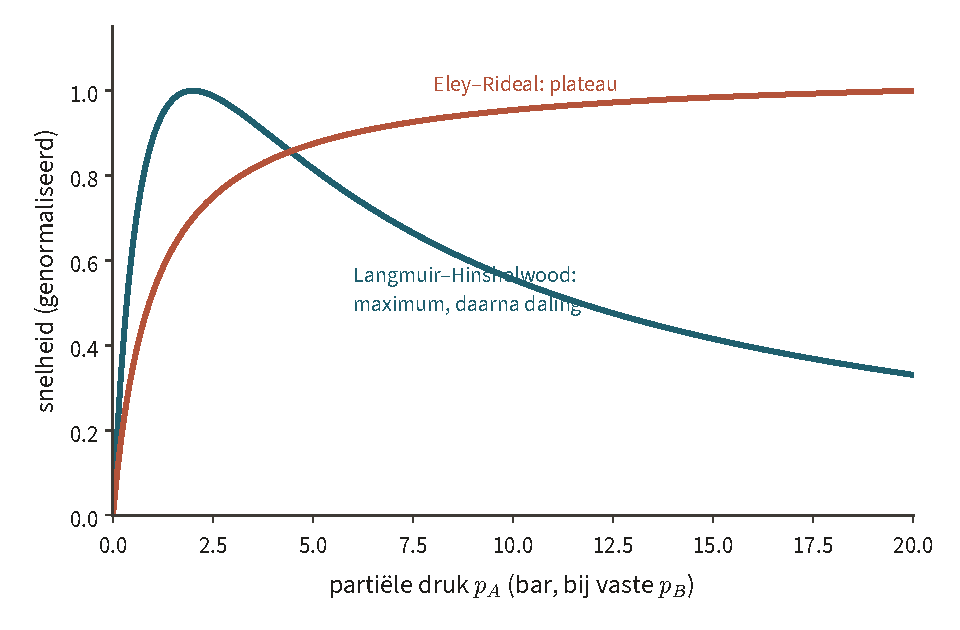
\includegraphics[width=0.7\linewidth]{Figuren/lh_er}
    \caption{Reactiesnelheid als functie van $p_A$ bij vaste $p_B$ volgens Langmuir--Hinshelwood (maximum, daarna daling door verdringing van $B$) en Eley--Rideal (monotone stijging naar een plateau).}
    \label{fig:lh-vs-er}
\end{figure}

\begin{toepassing}{Industri\"ele katalysatoren}
\begin{itemize}
\item \textbf{Haber--Bosch}: \ce{Fe3O4} met promotoren (\ce{K2O}, \ce{Al2O3}), \SIrange{400}{500}{\celsius}, \SIrange{150}{300}{\bar}. Snelheidsbepalend is de dissociatieve chemisorptie van \ce{N2}.
\item \textbf{Contactproces}: \ce{V2O5} voor \ce{SO2 -> SO3} bij \SIrange{400}{500}{\celsius}.
\item \textbf{Katalytisch kraken (FCC)}: zeolieten bij \SIrange{500}{600}{\celsius}. Thermisch kraken vroeg \SIrange{700}{800}{\celsius} en gaf veel cokes; de zeoliet verlaagt $E_a$ van meer dan \SI{250}{} tot ongeveer \SI{150}{\kilo\joule\per\mole} en is veel selectiever naar benzine.
\item \textbf{Driewegkatalysator}: Pt, Pd, Rh op \ce{Al2O3} oxideert CO en koolwaterstoffen en reduceert \ce{NO_x}, met Langmuir--Hinshelwood-kinetiek.
\item \textbf{Methanolsynthese}: \ce{Cu/ZnO/Al2O3} bij \SIrange{200}{300}{\celsius}.
\end{itemize}
\end{toepassing}

\section{Enzymkinetiek: Michaelis--Menten}
\label{sec:michaelis-menten}

Een enzym $E$ bindt zijn substraat $S$ tot een complex, dat het product vrijgeeft:
\begin{equation}
E + S \xrightleftharpoons[k_{-1}]{k_1} ES \xrightarrow{k_2} E + P.
\end{equation}
Steady state voor $ES$ en de massabalans $[E]_0 = [E] + [ES]$ geven de \emph{Michaelis--Mentenvergelijking}:
\begin{equation}
\boxed{\;r = \frac{r_{\max}\,[S]}{K_M + [S]}\;}
\qquad\text{met}\quad r_{\max} = k_2[E]_0, \quad K_M = \frac{k_{-1} + k_2}{k_1}.
\end{equation}
$K_M$ is de substraatconcentratie waarbij $r = r_{\max}/2$. Bij $[S] \ll K_M$ is de reactie eerste orde, bij $[S] \gg K_M$ nulde orde: alle enzymen zijn bezet. De vergelijking heeft exact de vorm van de Langmuir-isotherme (vergelijking~\eqref{eq:langmuir-isotherm}); in beide gevallen verzadigt een eindig aantal bindingsplaatsen. Een voorbeeld: met $K_M = \SI{2.0}{\milli\mole\per\litre}$ geeft $[S] = K_M$ de helft van $r_{\max}$, en tien keer meer substraat slechts \SI{91}{\percent} van $r_{\max}$.

\subsection{Diffusielimitatie}
\label{sec:diffusielimitatie}

Enzym en substraat moeten elkaar eerst vinden. Sneller dan diffusie toelaat, kan dat niet. Volgens Smoluchowski is de maximale bimoleculaire snelheidsconstante in oplossing
\begin{equation}
\boxed{\;k_D = 4\pi N_A\,(D_A+D_B)\,(r_A+r_B)\;}
\label{eq:smoluchowski}
\end{equation}
Voor een klein substraat ($D \approx \SI{1e-9}{\metre\squared\per\second}$, $r \approx \SI{0.5}{\nano\metre}$) en een enzym ($D \approx \SI{1e-10}{\metre\squared\per\second}$, $r \approx \SI{3}{\nano\metre}$) is $k_D \approx \SI{3e10}{\litre\per\mole\per\second}$. Enzymen die dit benaderen (carboanhydrase, triosefosfaatisomerase) heten \emph{diffusie-perfect}: elke ontmoeting leidt tot reactie.

De diffusieco\"effici\"ent van een bolvormig deeltje schat je met de \emph{vergelijking van Stokes--Einstein}:
\begin{equation}
\boxed{\;D = \frac{k_BT}{6\pi\eta r}\;}
\label{eq:stokes-einstein}
\end{equation}
Een opgeloste metaalcomplexkatalysator ($r \approx \SI{0.7}{\nano\metre}$) in tolueen ($\eta = \SI{6e-4}{\pascal\second}$) heeft $D \approx \SI{5e-10}{\metre\squared\per\second}$, vijf keer trager dan een klein substraatmolecule. In een grote reactor moet roeren, niet diffusie, de stoffen bijeenbrengen.

\section{Kinetiek en reactorontwerp}

Het vak Reactorentechnologie (Levenspiel) werkt reactorontwerp uit; hier enkel de kern. De benodigde verblijftijd $\tau$ volgt uit de snelheidswet. Voor een eerste-orde reactie met omzetting $X$:
\begin{equation}
\tau_\text{batch/PFR} = \frac{1}{k}\ln\frac{1}{1-X},
\qquad
\tau_\text{CSTR} = \frac{1}{k}\,\frac{X}{1-X}.
\end{equation}
In een ideaal geroerde tank (CSTR) heerst overal de lage eindconcentratie, in een batch- of propstroomreactor (PFR) daalt de concentratie geleidelijk. Voor $X = 0.90$ en $k = \SI{0.05}{\per\second}$ is $\tau_\text{PFR} = \SI{46}{\second}$ en $\tau_\text{CSTR} = \SI{180}{\second}$: de tank moet bijna vier keer groter zijn. Voor een tweede-orde reactie in een batchreactor is $\tau = X/(k[A]_0(1-X))$.


\section{Warmte en snelheid: wanneer een reactor op hol slaat}
\label{sec:runaway}

Een exotherme reactie warmt de reactor op, en een warmere reactor reageert sneller. Zolang de koeling de warmte afvoert, vindt de reactor een stabiel werkpunt. Lukt dat niet meer, dan versnelt de reactie zichzelf: \emph{thermische runaway}.

De warmteproductie is evenredig met de reactiesnelheid en stijgt dus exponentieel met de temperatuur:
\[
\dot Q_\mathrm{prod} = (-\Delta_rH)\,V\,k_0\,e^{-E_a/RT}\,c^n.
\]
De warmteafvoer door een koelmantel met koelmiddel op $T_c$ is lineair in $T$:
\[
\dot Q_\mathrm{afv} = UA\,(T - T_c).
\]
In een \emph{Semenovdiagram} (figuur~\ref{fig:semenov}) zie je beide curves. Waar ze snijden, is er evenwicht. Het onderste snijpunt is stabiel: wordt de reactor iets warmer, dan stijgt de afvoer sneller dan de productie en koelt hij terug af. Wordt het koelmiddel warmer of de koeling zwakker, dan schuift de rechte naar rechts tot ze de exponenti\"ele curve enkel nog raakt. Daarna is er geen snijpunt meer en loopt de temperatuur weg.

\begin{figure}[htb]
    \centering
    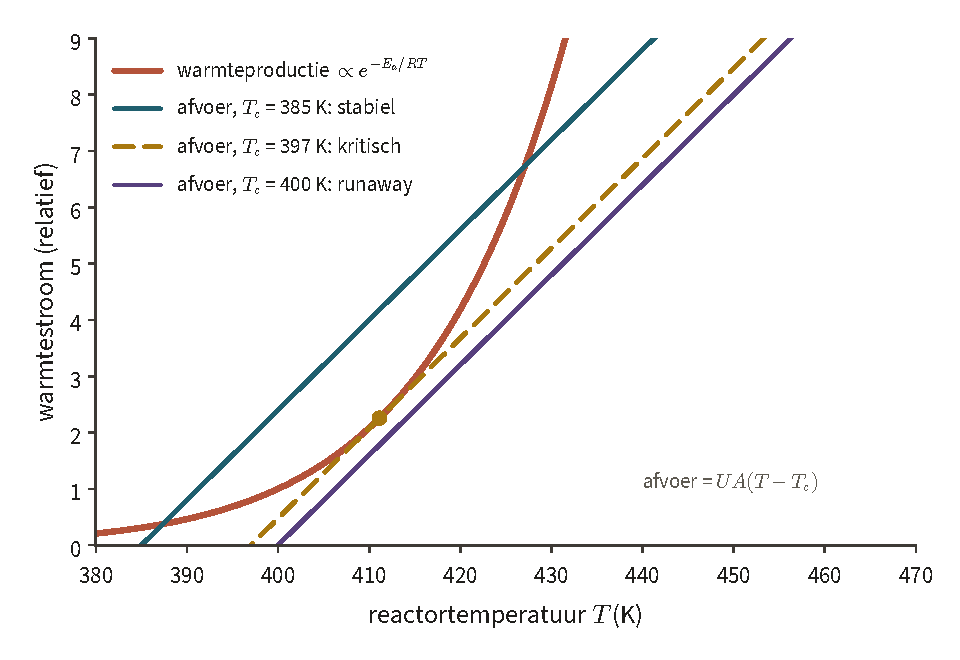
\includegraphics[width=0.7\linewidth]{Figuren/semenov}
    \caption{Semenovdiagram van een gekoelde reactor ($E_a = \SI{100}{\kilo\joule\per\mole}$, illustratieve waarden). Bij een koelmiddel van \SI{385}{\kelvin} is er een stabiel werkpunt. Bij \SI{397}{\kelvin} raakt de afvoerrechte de productiecurve: de kritische toestand. Bij \SI{400}{\kelvin} is er geen snijpunt meer: runaway.}
    \label{fig:semenov}
\end{figure}

Uit de raakvoorwaarde (gelijke waarde \'en gelijke helling) volgt een eenvoudige vuistregel: op het kritische punt ligt de reactortemperatuur ongeveer
\begin{equation}
\boxed{\;\Delta T_\mathrm{krit} \approx \frac{RT_c^2}{E_a}\;}
\label{eq:semenov}
\end{equation}
boven die van het koelmiddel. Voor $E_a = \SI{100}{\kilo\joule\per\mole}$ en $T_c = \SI{397}{\kelvin}$ is dat $8.314\cdot397^2/100\,000 = \SI{13}{\kelvin}$. Een reactor die meer dan een tiental graden warmer draait dan zijn koelmiddel, werkt dicht bij de grens. Hoe hoger $E_a$, hoe kleiner de marge.

\begin{toepassing}{Seveso en de veiligheid van chemische installaties}
Op 10 juli 1976 liep in een fabriek in Meda, bij Seveso (Itali\"e), een reactor voor trichloorfenol warm nadat de batch tijdens het weekend was stilgelegd zonder volledige afkoeling. Een exotherme nevenreactie versnelde zichzelf, de breekplaat opende en een wolk met dioxine (TCDD) kwam vrij over de omgeving. De ramp leidde tot de Europese Sevesorichtlijn, vandaag Seveso III. Bedrijven die grote hoeveelheden gevaarlijke stoffen behandelen, waaronder veel bedrijven in de haven van Antwerpen, moeten hun risico's op runaway en andere zware ongevallen analyseren en beheersen. De ingenieur gebruikt daarvoor de begrippen uit dit hoofdstuk en hoofdstuk~\ref{ch:energie}: de adiabatische temperatuurstijging (\S~\ref{sec:warmte-effecten}) zegt hoe ver de temperatuur kan oplopen, de activeringsenergie zegt hoe snel.
\end{toepassing}

\section{De brug tussen thermodynamica en kinetiek}
\label{sec:brug-thermo-kinetiek}

Voor een omkeerbare elementaire reactie $A \rightleftharpoons B$ is $K = k_1/k_{-1}$ (\S~\ref{sec:omkeerbare-reacties}). Beide constanten volgen Arrhenius, dus $\dd\ln k/\dd T = E_a/RT^2$ voor elk. Aftrekken geeft
\[
\frac{\dd{\ln K}}{\dd{T}} = \frac{E_{a,\text{heen}} - E_{a,\text{terug}}}{RT^2}.
\]
Vergelijk met Van 't Hoff (vergelijking~\eqref{eq:vanthoff-diff}), $\dd\ln K/\dd T = \Delta_rH^\circ/RT^2$:
\begin{equation}
\boxed{\;E_{a,\text{heen}} - E_{a,\text{terug}} \approx \Delta_r H^\circ\;}
\label{eq:Ea-verschil-drH}
\end{equation}
Dat zie je ook in figuur~\ref{fig:reactiecoordinaat-katalysator}: het hoogteverschil tussen begin- en eindtoestand is $\Delta_rH$, welke weg je ook neemt. Een exotherme reactie heeft dus altijd een lagere barri\`ere heen dan terug.

\subsection{Temperatuursgevoeligheid van exotherme en endotherme reacties}
\label{sec:temperatuursgevoeligheid}

Hoe groter $E_a$, hoe gevoeliger $k$ voor de temperatuur. Bij een exotherme evenwichtsreactie versnelt de \emph{terug}reactie dus sterker bij opwarming dan de heenreactie.

\begin{voorbeeld}{Ammoniaksynthese: heen- en terugreactie}
Met $E_{a,\text{heen}} \approx \SI{230}{\kilo\joule\per\mole}$ (\S~\ref{sec:ammoniak-arrhenius}) en $\Delta_rH^\circ \approx \SI{-92}{\kilo\joule\per\mole}$ is $E_{a,\text{terug}} = 230 + 92 = \SI{322}{\kilo\joule\per\mole}$. Van \SI{300}{\kelvin} naar \SI{700}{\kelvin} stijgt $k_\text{heen}$ met een factor $7.7\times10^{22}$, maar $k_\text{terug}$ met $1.1\times10^{32}$: tien grootteordes meer. Daarom daalt $K = k_\text{heen}/k_\text{terug}$ van ongeveer $6\times10^5$ naar $3\times10^{-4}$, precies wat Van 't Hoff ook gaf (\S~\ref{sec:vanthoff-reagerend}). Thermodynamica en kinetiek vertellen hetzelfde verhaal.
\end{voorbeeld}

\section{Industri\"ele toepassingen: een overzicht}

Bij elk proces zoekt de ingenieur een compromis tussen evenwicht (thermodynamica) en snelheid (kinetiek), en de katalysator verschuift dat compromis.
\begin{itemize}
\item \textbf{Haber--Bosch} en het \textbf{contactproces}: exotherm, dus lage $T$ geeft meer opbrengst, maar zonder \SIrange{400}{500}{\celsius} is de reactie te traag.
\item \textbf{Methanolsynthese}: ook exotherm, maar een actievere koperkatalysator laat \SIrange{200}{300}{\celsius} toe.
\item \textbf{Stoomreforming van methaan}: endotherm; zowel evenwicht als snelheid vragen \SIrange{800}{900}{\celsius}.
\item \textbf{Driewegkatalysator}: moet bij \SIrange{300}{800}{\celsius} meer dan \SI{95}{\percent} van CO, koolwaterstoffen en \ce{NO_x} omzetten; bij een koude start is hij nog niet actief.
\end{itemize}
Een betere katalysator laat een lagere temperatuur toe (meer opbrengst) zonder dat de reactie te traag wordt.


\section{Samenvatting en reflectie}

Met dit hoofdstuk is de cirkel rond. De thermodynamica (hoofdstukken~\ref{ch:energie} tot~\ref{ch:elektrochemie}) zegt welke toestand bereikbaar is; de kinetiek zegt hoe snel en via welke weg. Selectiviteit, katalyse en reactorveiligheid zijn telkens het resultaat van beide samen.

\begin{samenvatting}{Chemische kinetiek}
\begin{itemize}
\item Snelheidswet $r = k[A]^m[B]^n$; de orde volgt uit experiment. Ge\"integreerd: nulde orde lineair, eerste orde $\ln([A]_0/[A]) = kt$ met $t_{1/2} = \ln2/k$, tweede orde $1/[A] - 1/[A]_0 = kt$.
\item Arrhenius $k = A\,e^{-E_a/RT}$; $\ln k$ tegen $1/T$ geeft $E_a$. Botsingstheorie: $A = P\sigma\bar v_\mathrm{rel}N_A$ en $e^{-E_a/RT}$ is de fractie botsingen met genoeg energie.
\item Kinetische gastheorie: $\bar v = \sqrt{8RT/\pi M}$, vrije weglengte $\lambda = k_BT/(\sqrt2\sigma p)$ (\SI{68}{\nano\metre} voor lucht bij \SI{1}{\bar}); Graham: effusie $\propto 1/\sqrt M$.
\item Omkeerbare reacties naderen het evenwicht met tijdsconstante $1/(k_1+k_{-1})$, en $K = k_1/k_{-1}$.
\item Parallelle reacties: hoge $T$ bevoordeelt de reactie met de hoogste $E_a$. Reacties in serie: het tussenproduct heeft een optimale reactietijd.
\item Mechanismen: de steady-state-benadering en de snelheidsbepalende stap leveren de snelheidswet (ozon, Lindemann, Michaelis--Menten).
\item Een katalysator verlaagt $E_a$ in beide richtingen en verandert $K$ niet. Heterogene kinetiek bouwt op de Langmuir-isotherme (Langmuir--Hinshelwood, Eley--Rideal); transport door diffusie kan de snelheid beperken.
\item Runaway: de warmteproductie stijgt exponentieel, de afvoer lineair. Kritisch bij $T - T_c \approx RT_c^2/E_a$.
\item $E_{a,\mathrm{heen}} - E_{a,\mathrm{terug}} \approx \Delta_rH^\circ$: daarom verliest een exotherm evenwicht opbrengst bij hoge temperatuur.
\end{itemize}
\end{samenvatting}

\begin{reflectie}{Chemische kinetiek}
\begin{enumerate}
\item Waarom stijgt de reactiesnelheid veel sterker met de temperatuur dan de gemiddelde snelheid van de moleculen?
\item Waarom is de halfwaardetijd van een eerste-orde reactie onafhankelijk van de beginconcentratie, en die van een tweede-orde reactie niet?
\item Een katalysator versnelt de heenreactie met een factor duizend. Wat gebeurt er met de terugreactie, en waarom?
\item Waarom kan een hogere temperatuur de opbrengst van een tussenproduct in een serie-reactie verlagen, ook al gaat alles sneller?
\item Waarom werkt men bij ethyleenoxide niet gewoon bij een hogere temperatuur om de reactor kleiner te maken?
\item Waarom is een reactor met een reactie met hoge activeringsenergie gevoeliger voor runaway?
\item Waarom diffunderen gassen in de poriën van een katalysator anders dan in een buis van een centimeter?
\item Welke stap is snelheidsbepalend in een katalytische uitlaat net na een koude start, en welke als de motor warm is?
\end{enumerate}
\end{reflectie}

\newpage
\section{Oefeningen}

% Oefeningen bij dit hoofdstuk (ingevoegd achteraan het hoofdstuk met \input).
% Een oefening:  \begin{oefening}[titel] ... \end{oefening}   (boek en website)
% De oplossing:  \begin{oplossing} ... \end{oplossing}       (enkel website, dichtgeklapt)

Neem $g = \SI{9.81}{\metre\per\second\squared}$, $\sigma_{\text{water}} = \SI{72}{\milli\newton\per\metre}$ bij \SI{20}{\celsius}, $k_B = \SI{1.381e-23}{\joule\per\kelvin}$ en $R = \SI{8.314}{\joule\per\mole\per\kelvin}$.

\begin{oefening}[Hoeveel energie kost een wolk mist?]
Een ultrasone luchtbevochtiger vernevelt water tot fijne druppeltjes zonder het te verwarmen.

\begin{enumerate}
\item[(a)]
  Toon aan dat het totale oppervlak van een volume \(V\) verdeeld in bolletjes met straal \(r\) gelijk is aan \(A = 3V/r\).
\item[(b)]
  Bereken de minimale arbeid (de toename van de Gibbs-energie) om \(1.0\,\mathrm{L}\) water te vernevelen tot druppels met \(r = 1\,\mathrm{\mu m}\) en met \(r = 10\,\mathrm{\mu m}\).
\item[(c)]
  Vergelijk met de energie om \(1.0\,\mathrm{L}\) water \(5\,^\circ\mathrm{C}\) op te warmen en om het volledig te verdampen (\(\Delta_{\text{vap}}H \approx 2.45\,\mathrm{MJ/kg}\)). Waarom is een ultrasone bevochtiger zo zuinig?
\item[(d)]
  Waarom vloeien de druppels spontaan weer samen tot grotere druppels?
\end{enumerate}
\end{oefening}
\begin{oplossing}
\textbf{Resultaat:} (b) \textbf{216 J} voor \(1\,\mathrm{\mu m}\) en \textbf{22 J} voor \(10\,\mathrm{\mu m}\). (c) Opwarmen kost \(21\,\mathrm{kJ}\), verdampen \textbf{2.45 MJ}: vernevelen vraagt ruim tienduizend keer minder energie dan verdampen. (d) Samenvloeien verkleint het oppervlak en verlaagt dus \(G\).

\textbf{(a)} Het aantal druppels is \(N = V/(\tfrac{4}{3}\pi r^3)\), elk met oppervlak \(4\pi r^2\). Dus \(A = N\cdot 4\pi r^2 = 3V/r\). Hoe kleiner de druppels, hoe groter het oppervlak.

\textbf{(b)} Met vergelijking (9.1) is \(\Delta G = \sigma\,\Delta A\) (het oorspronkelijke oppervlak is verwaarloosbaar):

\begin{itemize}
\item
  \(r = 1\,\mathrm{\mu m}\): \(A = 3\times10^{-3}/10^{-6} = 3000\,\mathrm{m^2}\), \(\Delta G = 0.072 \times 3000 = 216\,\mathrm{J}\).
\item
  \(r = 10\,\mathrm{\mu m}\): \(A = 300\,\mathrm{m^2}\), \(\Delta G = 22\,\mathrm{J}\).
\end{itemize}

Eén liter water krijgt dus het oppervlak van een half voetbalveld.

\textbf{(c)} Opwarmen: \(Q = (1\,\mathrm{kg})(4184\,\mathrm{J/(kg\cdot K)})(5\,\mathrm{K}) = 21\,\mathrm{kJ}\). Verdampen: \(2.45\,\mathrm{MJ}\). Een verdampingsbevochtiger moet de volledige verdampingsenthalpie leveren (hoofdstuk 5), een ultrasone bevochtiger enkel de oppervlakte-energie en de verliezen in de piëzokristal. Het water verdampt later in de kamer met warmte uit de omgeving, zodat de lucht wat afkoelt.

\textbf{(d)} Bij samenvloeien daalt \(A\) en dus \(G = G_{\text{bulk}} + \sigma A\): het proces is spontaan. Fijne mist is enkel kinetisch stabiel, zolang de druppels elkaar weinig raken.
\end{oplossing}

\begin{oefening}[Capillariteit: van keukenpapier tot boomtoppen]
Gebruik de wet van Jurin (9.4).

\begin{enumerate}
\item[(a)]
  Hoe hoog stijgt water (\(\rho = 1000\,\mathrm{kg/m^3}\), \(\theta = 0^\circ\)) in een glazen capillair met een binnendiameter van \(0.20\,\mathrm{mm}\)?
\item[(b)]
  Herhaal voor kwik (\(\sigma = 485\,\mathrm{mN/m}\), \(\rho = 13600\,\mathrm{kg/m^3}\), \(\theta = 140^\circ\)) in hetzelfde capillair. Verklaar het teken.
\item[(c)]
  De vezels van keukenpapier vormen poriën met een straal van ongeveer \(25\,\mathrm{\mu m}\) en een contacthoek van \(30^\circ\). Hoe hoog kan water opstijgen in een verticaal opgehangen vel?
\item[(d)]
  De houtvaten (xyleem) van een boom hebben een straal van ongeveer \(20\,\mathrm{\mu m}\). Hoe hoog brengt capillariteit het water? Welke straal zou nodig zijn voor een sequoia van \(100\,\mathrm{m}\)? Wat besluit je?
\end{enumerate}
\end{oefening}
\begin{oplossing}
\textbf{Resultaat:} (a) \textbf{14.7 cm}. (b) \textbf{\ensuremath{-}5.6 cm}: kwik daalt. (c) Ongeveer \textbf{51 cm}. (d) Slechts \textbf{0.73 m}; voor \(100\,\mathrm{m}\) zou \(r = 0.15\,\mathrm{\mu m}\) nodig zijn: capillariteit alleen verklaart het watertransport in bomen niet.

\textbf{(a)} \(h = \dfrac{2\sigma\cos\theta}{\rho g r} = \dfrac{2(0.072)(1)}{(1000)(9.81)(1.0\times10^{-4})} = 0.147\,\mathrm{m}\).

\textbf{(b)} \(h = \dfrac{2(0.485)\cos 140^\circ}{(13600)(9.81)(1.0\times10^{-4})} = -0.056\,\mathrm{m}\). Omdat \(\cos 140^\circ < 0\), is de meniscus bol en wordt het kwik naar beneden gedrukt. Kwik bevochtigt glas niet: de cohesie tussen kwikatomen (metaalbinding, hoofdstuk 2) is veel sterker dan de adhesie aan glas. Daarom lees je een kwikthermometer af aan de top van een bolle meniscus.

\textbf{(c)} \(h = \dfrac{2(0.072)\cos 30^\circ}{(1000)(9.81)(25\times10^{-6})} = 0.51\,\mathrm{m}\). Het papier zuigt een plas dus gemakkelijk op, ook tegen de zwaartekracht in. Kleinere poriën zuigen hoger, maar de stroming wordt trager.

\textbf{(d)} \(h = 0.147 \times (100/20) = 0.73\,\mathrm{m}\). Voor \(h = 100\,\mathrm{m}\): \(r = 2\sigma/(\rho g h) = 1.5\times10^{-7}\,\mathrm{m}\). In werkelijkheid trekt de verdamping uit de bladeren het water omhoog: in de minuscule poriën van de celwanden in het blad (nanometers) houdt de oppervlaktespanning een sterke negatieve druk in stand, en de waterkolom hangt dankzij de cohesie tussen watermoleculen (waterstofbruggen, hoofdstuk 4) als een touw aan die menisci.
\end{oplossing}

\begin{oefening}[Waarom bruist spuitwater aan de wand van het glas?]
In een geopende fles spuitwater is het water oververzadigd met \(\mathrm{CO_2}\): het bevat evenveel opgelost gas als in evenwicht met ongeveer \(2.5\,\mathrm{bar}\) \(\mathrm{CO_2}\) (wet van Henry, hoofdstuk 5).

\begin{enumerate}
\item[(a)]
  Bereken met Young--Laplace de overdruk in een gasbelletje met straal \(10\,\mathrm{\mu m}\), \(1\,\mathrm{\mu m}\) en \(0.1\,\mathrm{\mu m}\).
\item[(b)]
  Een belletje kan enkel groeien als de \(\mathrm{CO_2}\)-druk erin lager is dan de evenwichtsdruk van \(2.5\,\mathrm{bar}\) die het opgeloste gas ``wil'' uitoefenen. Neem een atmosferische druk van \(1\,\mathrm{bar}\). Vanaf welke straal kan een belletje groeien?
\item[(c)]
  Waarom ontstaan bellen niet midden in het water maar op krasjes, stofvezels of een Mentos-snoepje?
\item[(d)]
  Waarom bruist een glas spuitwater sterker in een glas dat niet perfect gespoeld is?
\end{enumerate}
\end{oefening}
\begin{oplossing}
\textbf{Resultaat:} (a) \textbf{0.14}, \textbf{1.44} en \textbf{14.4 bar}. (b) Groei vanaf ongeveer \textbf{\(r \approx 1\,\mathrm{\mu m}\)}. (c) Krasjes en vezels bevatten al \textbf{gaszakjes} die groter zijn dan die kritische straal. (d) Vuil en vezels leveren zulke kiemen.

\textbf{(a)} \(\Delta p = 2\sigma/r\):

\begin{itemize}
\item
  \(r = 10\,\mathrm{\mu m}\): \(\Delta p = 2(0.072)/10^{-5} = 1.44\times10^{4}\,\mathrm{Pa} = 0.14\,\mathrm{bar}\)
\item
  \(r = 1\,\mathrm{\mu m}\): \(1.44\,\mathrm{bar}\)
\item
  \(r = 0.1\,\mathrm{\mu m}\): \(14.4\,\mathrm{bar}\)
\end{itemize}

\textbf{(b)} De druk in de bel is \(p_{\text{atm}} + 2\sigma/r\). Ze kan groeien zolang die druk kleiner is dan \(2.5\,\mathrm{bar}\), dus \(2\sigma/r < 1.5\,\mathrm{bar}\), of \(r > 2(0.072)/(1.5\times10^{5}) = 0.96\,\mathrm{\mu m}\). Een kleiner belletje heeft zo'n hoge inwendige druk dat het gas er volgens Henry terug uit oplost.

\textbf{(c)} Een belletje moet spontaan uit één molecule \(\mathrm{CO_2}\) groeien tot een micrometer: alle tussenstadia zijn onstabiel, dus dat gebeurt praktisch nooit. Een kras, een vezel of het ruwe oppervlak van een Mentos houdt echter kleine luchtzakjes vast die al groter zijn dan de kritische straal. Van daaruit groeien de bellen, laten ze los en blijft er een nieuw zakje achter: zo ontstaan de bekende parelsnoeren.

\textbf{(d)} Een perfect gladde, schone glazen wand heeft weinig kiemplaatsen. Restjes vaatdoek, stof of droogvlekken zijn ideale nucleatiekiemen. Champagneglazen worden daarom soms bewust met een laser op de bodem geëtst.
\end{oplossing}

\begin{oefening}[Twee zeepbellen: welke wint?]
Twee zeepbellen met straal \(1.0\,\mathrm{cm}\) en \(3.0\,\mathrm{cm}\) (\(\sigma = 25\,\mathrm{mN/m}\)) worden via een buisje met een kraantje met elkaar verbonden.

\begin{enumerate}
\item[(a)]
  Bereken de overdruk in elke bel. Waarom staat er \(4\sigma/r\) en niet \(2\sigma/r\)?
\item[(b)]
  Wat gebeurt er wanneer het kraantje opengaat? Waar stopt het proces?
\item[(c)]
  Verklaar met hetzelfde principe waarom ijskristallen in roomijs dat lang in de diepvries ligt groter en korreliger worden, en waarom schuim op bier na een tijdje uit minder, maar grotere bellen bestaat.
\end{enumerate}
\end{oefening}
\begin{oplossing}
\textbf{Resultaat:} (a) \textbf{10 Pa} in de kleine en \textbf{3.3 Pa} in de grote bel. (b) De \textbf{kleine bel loopt leeg} in de grote, tot er enkel een gebogen filmpje met de straal van de grote bel overblijft. (c) \textbf{Ostwald-rijping}: kleine deeltjes hebben een hogere druk of chemische potentiaal en verdwijnen ten voordele van grote.

\textbf{(a)} Een zeepbel heeft twee grensvlakken (binnen- en buitenkant van de film), zodat \(\Delta p = 4\sigma/r\):

\begin{itemize}
\item
  \(r = 1.0\,\mathrm{cm}\): \(\Delta p = 4(0.025)/0.010 = 10\,\mathrm{Pa}\)
\item
  \(r = 3.0\,\mathrm{cm}\): \(\Delta p = 3.3\,\mathrm{Pa}\)
\end{itemize}

\textbf{(b)} Gas stroomt van hoge naar lage druk: de kleine bel loopt leeg in de grote. Daardoor wordt de kleine bel nog kleiner, haar druk stijgt nog meer, en het proces versnelt. Het stopt pas wanneer van de kleine bel een kapje over is met dezelfde kromtestraal als de grote bel. Dit is tegenintuïtief (je zou verwachten dat de drukken gelijk worden bij gelijke bellen), maar volgt rechtstreeks uit Young--Laplace en uit de daling van het totale oppervlak, dus van \(G\).

\textbf{(c)} Kleine ijskristallen en kleine gasbellen hebben een sterkere kromming en dus een hogere chemische potentiaal (vergelijk met de hogere druk in de bel). Watermoleculen gaan van kleine naar grote kristallen, gas diffundeert van kleine naar grote bellen. Het totale grensvlak en dus \(G\) dalen. Ijsfabrikanten voegen stabilisatoren toe en raden aan de diepvries niet te vaak te openen: elke temperatuurschommeling versnelt de rijping.
\end{oplossing}

\begin{oefening}[Wast warm water beter? Oppervlaktespanning en temperatuur]
Voor water geldt \(\sigma = 72.75\,\mathrm{mN/m}\) bij \(20\,^\circ\mathrm{C}\), met \(V_m = 18.05\,\mathrm{cm^3/mol}\) en \(T_c = 647.1\,\mathrm{K}\).

\begin{enumerate}
\item[(a)]
  Bereken de constante \(k\) in de vergelijking van Eötvös (9.2) uit deze gegevens.
\item[(b)]
  Voorspel \(\sigma\) bij \(60\,^\circ\mathrm{C}\) (\(V_m = 18.32\,\mathrm{cm^3/mol}\)) en bij \(80\,^\circ\mathrm{C}\) (\(V_m = 18.54\,\mathrm{cm^3/mol}\)). De gemeten waarden zijn \(66.2\) en \(62.6\,\mathrm{mN/m}\). Hoe goed is de voorspelling?
\item[(c)]
  Waarom daalt de oppervlaktespanning met de temperatuur, en wat gebeurt er bij het kritische punt?
\item[(d)]
  Geef twee redenen waarom een afwas in warm water beter lukt dan in koud water.
\end{enumerate}
\end{oefening}
\begin{oplossing}
\textbf{Resultaat:} (a) \(k = 1.41\times10^{-7}\,\mathrm{J/(K\cdot mol^{2/3})}\). (b) Voorspeld \textbf{63.9} en \textbf{59.3 mN/m}: ongeveer \textbf{4--5 \% te laag}. (c) Zwakkere cohesie ten opzichte van de thermische energie; \(\sigma \to 0\) bij \(T_c\). (d) Lagere \(\sigma\) en vet dat smelt en sneller oplost.

\textbf{(a)} \(k = \dfrac{\sigma V_m^{2/3}}{T_c - T} = \dfrac{(0.07275)(18.05\times10^{-6})^{2/3}}{647.1 - 293.15} = 1.41\times10^{-7}\,\mathrm{J/(K\cdot mol^{2/3})}\), dicht bij de ``universele'' waarde van ongeveer \(2.1\times10^{-7}\) voor niet-geassocieerde vloeistoffen. Water wijkt af door de waterstofbruggen.

\textbf{(b)} \(\sigma = k(T_c - T)/V_m^{2/3}\):

\begin{itemize}
\item
  \(60\,^\circ\mathrm{C}\): \(\sigma = 63.9\,\mathrm{mN/m}\) (gemeten \(66.2\), afwijking \(-3.5\,\%\))
\item
  \(80\,^\circ\mathrm{C}\): \(\sigma = 59.3\,\mathrm{mN/m}\) (gemeten \(62.6\), afwijking \(-5\,\%\))
\end{itemize}

Een empirische correlatie met één constante, gefit op één punt, extrapoleert dus redelijk maar niet perfect. Daarom gebruikt men in de praktijk varianten met een gecorrigeerde \(T_c\) (bijvoorbeeld \(T_c - 6\,\mathrm{K}\)).

\textbf{(c)} Bij hogere temperatuur is de thermische energie groter ten opzichte van de intermoleculaire aantrekking (hoofdstuk 4); het kost minder Gibbs-energie om een molecule naar het oppervlak te brengen. Bij \(T_c\) verdwijnt het onderscheid tussen vloeistof en damp (hoofdstuk 5), er is geen grensvlak meer en \(\sigma = 0\).

\textbf{(d)} Water met een lagere oppervlaktespanning bevochtigt borden en vezels beter en dringt dieper in kleine spleten. Daarnaast smelten vetten met een smeltpunt boven kamertemperatuur, verlopen oplos- en diffusieprocessen sneller (Stokes--Einstein: \(D \propto T/\eta\), en \(\eta\) daalt sterk), en werkt het afwasmiddel sneller. Het afwasmiddel zelf verlaagt \(\sigma\) nog veel meer dan de temperatuur.
\end{oplossing}

\begin{oefening}[Hoeveel afwasmiddel heb je nodig? CMC en micellen]
Natriumdodecylsulfaat (SDS, \(M = 288.4\,\mathrm{g/mol}\)) heeft een CMC van \(8.2\times10^{-3}\,\mathrm{mol/L}\) bij \(25\,^\circ\mathrm{C}\) en vormt micellen van gemiddeld \(62\) moleculen.

\begin{enumerate}
\item[(a)]
  Hoeveel gram SDS moet je minstens in een afwasbak van \(15\,\mathrm{L}\) doen om de CMC te bereiken? Moderne vaatwasmiddelen bevatten vooral niet-ionische surfactanten met een CMC rond \(1\times10^{-4}\,\mathrm{mol/L}\) (\(M \approx 530\,\mathrm{g/mol}\)). Hoeveel gram is dan nodig?
\item[(b)]
  Een oplossing bevat \(1.0\times10^{-2}\,\mathrm{mol/L}\) SDS. Hoeveel SDS is vrij opgelost, en hoeveel micellen zijn er per liter?
\item[(c)]
  In een eenvoudig model geldt \(\Delta G^\circ_{\text{mic}} \approx RT\ln x_{\text{CMC}}\), met \(x_{\text{CMC}}\) de molfractie surfactant bij de CMC. Bereken \(\Delta G^\circ_{\text{mic}}\) per mol surfactant. Met \(\Delta H^\circ_{\text{mic}} \approx -1.5\,\mathrm{kJ/mol}\): bereken \(T\Delta S^\circ_{\text{mic}}\). Wat is de drijvende kracht?
\item[(d)]
  Waarom wordt een afwasmiddel minder doeltreffend in een gootsteen vol vet?
\end{enumerate}
\end{oefening}
\begin{oplossing}
\textbf{Resultaat:} (a) \textbf{35 g} SDS, maar slechts ongeveer \textbf{0.8 g} niet-ionische surfactant. (b) Vrij: \textbf{\(8.2\times10^{-3}\,\mathrm{mol/L}\)}; micellen: \textbf{\(2.9\times10^{-5}\,\mathrm{mol/L}\)} (\(1.7\times10^{19}\) per liter). (c) \(\Delta G^\circ_{\text{mic}} \approx\) \textbf{\ensuremath{-}21.9 kJ/mol} en \(T\Delta S^\circ \approx\) \textbf{+20 kJ/mol}: entropisch gedreven. (d) Het vet verbruikt de surfactant tot de vrije concentratie onder de CMC zakt.

\textbf{(a)} SDS: \(15\,\mathrm{L} \times 8.2\times10^{-3}\,\mathrm{mol/L} \times 288.4\,\mathrm{g/mol} = 35\,\mathrm{g}\), een flinke scheut. Niet-ionisch: \(15 \times 1\times10^{-4} \times 530 = 0.8\,\mathrm{g}\). Een lagere CMC betekent dat veel minder product nodig is om micellen te vormen; daarom zijn moderne, geconcentreerde wasmiddelen zo zuinig. Een lange hydrofobe staart en het ontbreken van een geladen kop (geen elektrostatische afstoting tussen de koppen) verlagen de CMC.

\textbf{(b)} Boven de CMC blijft de vrije concentratie gelijk aan de CMC: \(8.2\times10^{-3}\,\mathrm{mol/L}\). De rest, \(1.8\times10^{-3}\,\mathrm{mol/L}\), zit in micellen: \(1.8\times10^{-3}/62 = 2.9\times10^{-5}\,\mathrm{mol/L}\) micellen, of \(1.7\times10^{19}\) micellen per liter.

\textbf{(c)} Met \(55.5\,\mathrm{mol/L}\) water: \(x_{\text{CMC}} = 8.2\times10^{-3}/55.5 = 1.48\times10^{-4}\), dus \(\Delta G^\circ_{\text{mic}} = (8.314)(298.15)\ln(1.48\times10^{-4}) = -21.9\,\mathrm{kJ/mol}\). Dan \(T\Delta S^\circ = \Delta H^\circ - \Delta G^\circ = -1.5 + 21.9 = +20.4\,\mathrm{kJ/mol}\). Bijna de volledige drijvende kracht is entropisch: het hydrofoob effect (§9.4.2). De geordende watermoleculen rond de koolwaterstofstaarten komen vrij wanneer de staarten in de micel verdwijnen (hoofdstuk 3, \(\Delta G = \Delta H - T\Delta S\)).

\textbf{(d)} Vet wordt opgelost in de kern van de micellen en surfactant adsorbeert aan het grote vet--watergrensvlak. Dat onttrekt surfactant aan de oplossing. Zakt de vrije concentratie onder de CMC, dan verdwijnen de micellen, stijgt de oppervlaktespanning en komt het vet terug vrij. Bij een zeer vette afwas moet je dus water verversen of meer middel toevoegen.
\end{oplossing}

\begin{oefening}[De zeta-potentiaal van klei meten met elektroforese]
Kleideeltjes in rivierwater bewegen in een elektrisch veld van \(1000\,\mathrm{V/m}\) met een snelheid van \(35\,\mathrm{\mu m/s}\) naar de positieve elektrode. Na toevoegen van \(10\,\mathrm{mmol/L}\) \(\mathrm{CaCl_2}\) daalt de snelheid tot \(9.5\,\mathrm{\mu m/s}\). Volgens de vergelijking van Smoluchowski is de elektroforetische mobiliteit \(u = v/E = \varepsilon_r\varepsilon_0\zeta/\eta\), met voor water \(\varepsilon_r = 78.5\), \(\varepsilon_0 = 8.854\times10^{-12}\,\mathrm{F/m}\) en \(\eta = 8.9\times10^{-4}\,\mathrm{Pa\,s}\).

\begin{enumerate}
\item[(a)]
  Wat is het teken van de oppervlaktelading van de kleideeltjes?
\item[(b)]
  Bereken de zeta-potentiaal voor en na toevoegen van \(\mathrm{CaCl_2}\).
\item[(c)]
  Voorspel de stabiliteit van de dispersie in beide gevallen.
\item[(d)]
  Waarom is \(\mathrm{Ca^{2+}}\) veel doeltreffender dan \(\mathrm{Na^+}\), en waarom gebruiken drinkwaterbedrijven \(\mathrm{Al^{3+}}\)-zouten?
\item[(e)]
  Waarom is het water aan de monding van een rivier in de zee vaak troebel en slibt de haven er dicht?
\end{enumerate}
\end{oefening}
\begin{oplossing}
\textbf{Resultaat:} (a) \textbf{Negatief}. (b) \(\zeta \approx\) \textbf{\ensuremath{-}45 mV} voor en \textbf{\ensuremath{-}12 mV} na toevoegen. (c) Eerst \textbf{stabiel} (\(|\zeta| > 30\,\mathrm{mV}\)), daarna bijna aan de grens van \textbf{snelle coagulatie}. (d) Meerwaardige tegenionen comprimeren de dubbellaag veel sterker. (e) Zeewater is een zoutoplossing: de klei coaguleert en bezinkt.

\textbf{(a)} De deeltjes bewegen naar de positieve elektrode: ze zijn negatief geladen. Klei krijgt die lading door isomorfe substitutie (\(\mathrm{Al^{3+}}\) in plaats van \(\mathrm{Si^{4+}}\) in het kristalrooster) en door ionisatie van randgroepen.

\textbf{(b)} \(\zeta = \dfrac{u\,\eta}{\varepsilon_r\varepsilon_0}\) met \(\varepsilon_r\varepsilon_0 = 6.95\times10^{-10}\,\mathrm{F/m}\):

\begin{itemize}
\item
  voor: \(u = 3.5\times10^{-8}\,\mathrm{m^2/(V\cdot s)}\), \(\zeta = \dfrac{(3.5\times10^{-8})(8.9\times10^{-4})}{6.95\times10^{-10}} = 0.045\,\mathrm{V}\), dus \(\zeta = -45\,\mathrm{mV}\)
\item
  na: \(u = 9.5\times10^{-9}\,\mathrm{m^2/(V\cdot s)}\), \(\zeta = -12\,\mathrm{mV}\)
\end{itemize}

\textbf{(c)} Met \(|\zeta| = 45\,\mathrm{mV}\) is er een hoge DLVO-energiedrempel en blijft de klei zweven: het water blijft troebel. Bij \(12\,\mathrm{mV}\) is de afstoting bijna verdwenen en domineert de Van der Waals-aantrekking: de deeltjes klonteren samen tot vlokken die bezinken.

\textbf{(d)} Een tegenion met een hogere lading schermt de oppervlaktelading veel efficiënter af: de dubbellaag wordt dunner (kleinere Debye-lengte) en \(\zeta\) daalt, en tweewaardige ionen worden bovendien sterker in de Stern-laag gebonden. Empirisch neemt de benodigde coagulatieconcentratie zeer sterk af met de lading van het tegenion (de regel van Schulze--Hardy): \(\mathrm{Al^{3+}}\) werkt al bij veel lagere doses dan \(\mathrm{Ca^{2+}}\), en die op hun beurt veel beter dan \(\mathrm{Na^+}\). Bovendien vormt \(\mathrm{Al^{3+}}\) in water vlokkig \(\mathrm{Al(OH)_3}\) dat de deeltjes mee insluit.

\textbf{(e)} Zeewater bevat ongeveer \(0.5\,\mathrm{mol/L}\) \(\mathrm{NaCl}\) en daarnaast \(\mathrm{Mg^{2+}}\) en \(\mathrm{Ca^{2+}}\). Waar rivierwater zich met zeewater mengt, coaguleert de klei en bezinkt ze. Zo ontstaan slikken en schorren, en moet een haven als Antwerpen of Zeebrugge voortdurend gebaggerd worden.
\end{oplossing}

\begin{oefening}[Mayonaise en dressing: grensvlak en HLB]
Mayonaise bevat ongeveer \(80\,\mathrm{vol\%}\) olie in de vorm van druppels met een straal van ongeveer \(1\,\mathrm{\mu m}\) in een waterfase met eigeel en azijn.

\begin{enumerate}
\item[(a)]
  Bereken het olie--watergrensvlak in \(1\,\mathrm{L}\) mayonaise.
\item[(b)]
  Bereken de grensvlakenergie bij een grensvlakspanning van \(30\,\mathrm{mN/m}\) (zonder emulgator) en \(5\,\mathrm{mN/m}\) (met eigeel). Is mayonaise thermodynamisch stabiel?
\item[(c)]
  Een fabrikant wil een vinaigrette (O/W) stabiliseren met een mengsel van Span 80 (HLB \(4.3\)) en Tween 80 (HLB \(15.0\)) en mikt op een HLB van \(10\). Het HLB-getal van een mengsel is het massagewogen gemiddelde. Welk massapercentage Tween 80 is nodig?
\item[(d)]
  Welke emulgator (Span 80 alleen of Tween 80 alleen) kies je voor een W/O-product zoals een vette handcrème of margarine? Verklaar met de structuur van de moleculen.
\end{enumerate}
\end{oefening}
\begin{oplossing}
\textbf{Resultaat:} (a) \textbf{2400 m\ensuremath{^{2}}} per liter. (b) \textbf{72 J} zonder en \textbf{12 J} met emulgator; mayonaise blijft \textbf{thermodynamisch onstabiel}, maar is kinetisch stabiel. (c) Ongeveer \textbf{53 \%} Tween 80. (d) \textbf{Span 80} (HLB 4.3).

\textbf{(a)} Met \(A = 3V_{\text{olie}}/r\) (oefening 9.1): \(A = 3(0.80\times10^{-3}\,\mathrm{m^3})/(1\times10^{-6}\,\mathrm{m}) = 2400\,\mathrm{m^2}\).

\textbf{(b)} \(G_{\text{grensvlak}} = \sigma A\): \(0.030 \times 2400 = 72\,\mathrm{J}\) zonder emulgator, \(0.005 \times 2400 = 12\,\mathrm{J}\) met eigeel. Ook met emulgator blijft \(\Delta G > 0\) ten opzichte van een gescheiden laag olie en water: de emulsie is thermodynamisch onstabiel (§9.6). Lecithine en eiwitten uit het eigeel verlagen de energie die je met de garde moet leveren en vormen vooral een beschermende laag die het samenvloeien van druppels kinetisch verhindert. Bij te veel opwarmen of invriezen breekt die laag en ``schift'' de mayonaise.

\textbf{(c)} Met \(w\) de massafractie Tween 80: \(15.0\,w + 4.3(1 - w) = 10\), dus \(w = 5.7/10.7 = 0.53\), of \(53\,\%\) Tween 80 en \(47\,\%\) Span 80. Mengsels van een hydrofiele en een lipofiele emulgator laten toe het HLB-getal fijn af te stemmen.

\textbf{(d)} Voor een W/O-emulsie is een lipofiele emulgator met HLB \(3\)--\(6\) nodig: Span 80 (sorbitanmono-oleaat) heeft een kleine polaire kop en een lange oliezuurstaart, en buigt het grensvlak rond de waterdruppels. Tween 80 is hetzelfde molecule met lange polyethyleenoxideketens aan de kop: sterk hydrofiel, en dus geschikt voor O/W (melk, dressing, vloeibare geneesmiddelen).
\end{oplossing}

\begin{oefening}[Waarom roomt gehomogeniseerde melk niet op?]
Vetbolletjes in rauwe melk hebben een straal van ongeveer \(1.5\,\mathrm{\mu m}\); na homogeniseren is dat ongeveer \(0.25\,\mathrm{\mu m}\). De dichtheid van melkvet is \(920\,\mathrm{kg/m^3}\), die van de waterfase \(1030\,\mathrm{kg/m^3}\), en de viscositeit van de waterfase \(2.0\times10^{-3}\,\mathrm{Pa\,s}\). De snelheid waarmee een bolletje opstijgt is gegeven door de wet van Stokes, \(v = 2r^2\Delta\rho\,g/(9\eta)\).

\begin{enumerate}
\item[(a)]
  Bereken de opstijgsnelheid (in cm per dag) voor beide groottes.
\item[(b)]
  Bereken met Stokes--Einstein (hoofdstuk 8, vergelijking (8.35)) de diffusiecoëfficiënt bij \(20\,^\circ\mathrm{C}\), en de typische afstand die een bolletje door Brownse beweging aflegt in één dag (\(\sqrt{2Dt}\)).
\item[(c)]
  Verklaar waarom op rauwe melk na een dag een roomlaag ligt, maar niet op gehomogeniseerde melk.
\item[(d)]
  Waarom vallen deeltjes kleiner dan \(1\,\mathrm{\mu m}\) onder de definitie van een colloïde (§9.5)?
\end{enumerate}
\end{oefening}
\begin{oplossing}
\textbf{Resultaat:} (a) \textbf{2.3 cm/dag} voor rauwe en \textbf{0.065 cm/dag} (0.65 mm) voor gehomogeniseerde melk. (b) \(D = 7.2\times10^{-14}\) en \(4.3\times10^{-13}\,\mathrm{m^2/s}\); per dag ongeveer \textbf{0.11 mm} en \textbf{0.27 mm}. (c) Kleine bolletjes stijgen 36 keer trager en Brownse beweging en convectie houden ze verspreid. (d) Bij die grootte wint de thermische beweging het van de zwaartekracht.

\textbf{(a)} Met \(\Delta\rho = 110\,\mathrm{kg/m^3}\):

\begin{itemize}
\item
  \(r = 1.5\,\mathrm{\mu m}\): \(v = \dfrac{2(1.5\times10^{-6})^2(110)(9.81)}{9(2.0\times10^{-3})} = 2.7\times10^{-7}\,\mathrm{m/s} = 2.3\,\mathrm{cm/dag}\)
\item
  \(r = 0.25\,\mathrm{\mu m}\): \(v = 7.5\times10^{-9}\,\mathrm{m/s} = 0.065\,\mathrm{cm/dag}\)
\end{itemize}

Omdat \(v \propto r^2\), maakt een zes keer kleinere straal het opromen 36 keer trager.

\textbf{(b)} \(D = \dfrac{k_BT}{6\pi\eta r}\):

\begin{itemize}
\item
  \(r = 1.5\,\mathrm{\mu m}\): \(D = 7.2\times10^{-14}\,\mathrm{m^2/s}\), \(\sqrt{2D\cdot 86400\,\mathrm{s}} = 0.11\,\mathrm{mm}\)
\item
  \(r = 0.25\,\mathrm{\mu m}\): \(D = 4.3\times10^{-13}\,\mathrm{m^2/s}\), \(\sqrt{2Dt} = 0.27\,\mathrm{mm}\)
\end{itemize}

\textbf{(c)} In rauwe melk stijgen de bolletjes in een dag enkele centimeter, veel meer dan de Brownse verplaatsing: er vormt zich een roomlaag (in werkelijkheid nog sneller, omdat de bolletjes samenklonteren tot grotere trossen). In gehomogeniseerde melk stijgen ze minder dan een millimeter per dag, vergelijkbaar met de willekeurige Brownse verplaatsing; kleine temperatuurstromingen in de koelkast mengen de melk bovendien voortdurend. Na enkele weken zou je nog altijd geen duidelijke roomlaag zien, maar dan is de melk allang bedorven.

\textbf{(d)} Een deeltje is colloïdaal wanneer de Brownse beweging de zwaartekracht ruwweg in evenwicht houdt. Uit (a) en (b) zie je dat dit omslagpunt rond \(1\,\mathrm{\mu m}\) ligt: kleinere deeltjes blijven verspreid, grotere zakken of stijgen merkbaar.
\end{oplossing}

\begin{oefening}[Pesticiden uit drinkwater halen met actieve kool]
Een drinkwaterbedrijf behandelt \(1.0\times10^{5}\,\mathrm{m^3}\) water per dag dat \(2.0\,\mathrm{\mu g/L}\) van een pesticide bevat. De norm is \(0.1\,\mathrm{\mu g/L}\). De adsorptie op actieve kool volgt een Langmuir-isotherme (§9.3) \(q = q_{\max}Kc/(1 + Kc)\), met \(q_{\max} = 50\,\mathrm{mg/g}\), \(K = 20\,\mathrm{L/mg}\) en \(c\) in mg/L.

\begin{enumerate}
\item[(a)]
  Bereken de belading \(q\) van de kool in evenwicht met \(2.0\,\mathrm{\mu g/L}\) en met \(0.1\,\mathrm{\mu g/L}\). In welk gebied van de isotherme zit je?
\item[(b)]
  Methode A: men roert poederkool door het water tot de concentratie \(0.1\,\mathrm{\mu g/L}\) bereikt. Hoeveel gram kool is per liter nodig, en hoeveel ton per dag?
\item[(c)]
  Methode B: het water stroomt door een vast bed korrelkool. Voor het bed doorbreekt, staat de kool in evenwicht met de ingangsconcentratie. Hoeveel kool wordt dan per dag verbruikt?
\item[(d)]
  Verklaar waarom methode B zoveel zuiniger is. Welk verband zie je met tegenstroomprocessen in de scheidingstechniek?
\end{enumerate}
\end{oefening}
\begin{oplossing}
\textbf{Resultaat:} (a) \(q = 1.9\,\mathrm{mg/g}\) bij \(2.0\,\mathrm{\mu g/L}\) en \textbf{0.10 mg/g} bij \(0.1\,\mathrm{\mu g/L}\): het lineaire gebied. (b) \textbf{0.019 g/L}, of ongeveer \textbf{1.9 ton per dag}. (c) Ongeveer \textbf{99 kg per dag}. (d) In een vast bed raakt de kool beladen bij de \textbf{hoge ingangsconcentratie}.

\textbf{(a)} \(2.0\,\mathrm{\mu g/L} = 0.0020\,\mathrm{mg/L}\), dus \(Kc = 0.040\) en \(q = 50 \times 0.040/1.040 = 1.92\,\mathrm{mg/g}\). Bij \(0.1\,\mathrm{\mu g/L}\): \(Kc = 0.002\) en \(q = 0.0998\,\mathrm{mg/g}\). Omdat \(Kc \ll 1\) zit je in het lineaire gebied \(q \approx q_{\max}Kc\): de belading is evenredig met de concentratie, en de kool is nog bijna leeg (\(\theta < 4\,\%\)).

\textbf{(b)} Een massabalans per liter: \(m\,q_{\text{eind}} = c_0 - c_{\text{eind}}\), dus \(m = (0.0020 - 0.0001)/0.0998 = 0.019\,\mathrm{g/L}\). Voor \(10^{8}\,\mathrm{L}\) per dag: \(1.9\times10^{6}\,\mathrm{g} = 1.9\,\mathrm{ton}\) kool per dag.

\textbf{(c)} Te verwijderen: \((0.0020 - 0.0001)\,\mathrm{mg/L} \times 10^{8}\,\mathrm{L} = 1.9\times10^{5}\,\mathrm{mg}\) per dag. Met \(q = 1.92\,\mathrm{mg/g}\): \(9.9\times10^{4}\,\mathrm{g} = 99\,\mathrm{kg}\) per dag.

\textbf{(d)} In methode A eindigt alle kool in evenwicht met het gezuiverde water, bij de laagste concentratie en dus de laagste belading. In het vaste bed ziet de kool aan de ingang eerst het vervuilde water en raakt ze tot een twintig keer hogere belading gevuld, terwijl de laatste lagen kool het water tot onder de norm zuiveren. Dat is hetzelfde principe als bij tegenstroomextractie of een absorptiekolom: het scheidingsmiddel verlaat het toestel in evenwicht met de rijkste stroom. Daarom gebruiken drinkwaterbedrijven korrelkoolfilters, en poederkool enkel bij een plotse, tijdelijke vervuiling.
\end{oplossing}

\begin{oefening}[Lopen op water]
Een schaatsenrijder (het insect) heeft een massa van ongeveer \(10\,\mathrm{mg}\) en raakt het water over een totale beenlengte van ongeveer \(3\,\mathrm{cm}\). De oppervlaktespanning kan per eenheid contactlengte een verticale kracht van hoogstens \(2\sigma\) leveren (één bijdrage aan elke kant van het been).

\begin{enumerate}
\item[(a)]
  Bereken de maximale draagkracht van het wateroppervlak en vergelijk met het gewicht van het insect.
\item[(b)]
  Herhaal met zeepwater (\(\sigma = 30\,\mathrm{mN/m}\)). Waarom zakt het insect in de praktijk toch door wanneer je een druppel afwasmiddel toevoegt?
\item[(c)]
  Kan een stalen naald (\(\rho = 7900\,\mathrm{kg/m^3}\), lengte \(3\,\mathrm{cm}\), diameter \(0.5\,\mathrm{mm}\)) op water drijven? Waarom moet je ze voorzichtig neerleggen?
\end{enumerate}
\end{oefening}
\begin{oplossing}
\textbf{Resultaat:} (a) Ongeveer \textbf{4.3 mN}, ruim \textbf{40 keer} het gewicht van \(0.098\,\mathrm{mN}\). (b) Nog \(1.8\,\mathrm{mN}\), maar het afwasmiddel laat de waterafstotende beentjes \textbf{bevochtigen}. (c) Ja: gewicht \textbf{0.46 mN} tegenover 4.3 mN, op voorwaarde dat het oppervlak niet doorbroken wordt.

\textbf{(a)} \(F_{\max} = 2\sigma L = 2(0.072)(0.03) = 4.3\times10^{-3}\,\mathrm{N}\). Het gewicht is \(mg = (10\times10^{-6})(9.81) = 9.8\times10^{-5}\,\mathrm{N}\). Het insect gebruikt dus maar een fractie van de draagkracht en kan zelfs springen zonder door het oppervlak te gaan.

\textbf{(b)} \(F_{\max} = 2(0.030)(0.03) = 1.8\,\mathrm{mN}\), nog altijd veel meer dan het gewicht. De echte reden is de bevochtiging: de beentjes zijn bedekt met waterafstotende haartjes (een grote contacthoek), zodat het wateroppervlak een kuiltje vormt in plaats van rond het been te sluiten. Surfactant adsorbeert op die haartjes, de contacthoek daalt, het water bevochtigt het been en de opwaartse component van de kracht verdwijnt. Daarom zijn zeep en olievlekken dodelijk voor waterinsecten.

\textbf{(c)} \(V = \pi(0.25\times10^{-3})^2(0.03) = 5.9\times10^{-9}\,\mathrm{m^3}\), \(m = 46\,\mathrm{mg}\), gewicht \(0.46\,\mathrm{mN}\), kleiner dan de \(4.3\,\mathrm{mN}\) die het oppervlak kan dragen. De naald drijft dus, ook al is staal acht keer zwaarder dan water. Leg je ze schuin of met een tik neer, dan breekt ze door het oppervlak: eens ondergedompeld is er geen grensvlak meer dat ze draagt, en zinkt ze.
\end{oplossing}

\begin{oefening}[Geïntegreerde case: van rivierwater naar drinkwater]
Een drinkwaterbedrijf zuivert \(1.0\times10^{5}\,\mathrm{m^3}\) rivierwater per dag. Het water is troebel door kleideeltjes met een diameter van \(1\,\mathrm{\mu m}\) (\(\rho = 2600\,\mathrm{kg/m^3}\)) en een zeta-potentiaal van \(-35\,\mathrm{mV}\). Neem \(\eta = 1.0\times10^{-3}\,\mathrm{Pa\,s}\) en de wet van Stokes uit oefening 9.9.

\begin{enumerate}
\item[(a)]
  Hoe lang duurt het voor een kleideeltje \(3\,\mathrm{m}\) diep bezinkt in een bezinkbekken? Waarom bezinkt het in de praktijk helemaal niet?
\item[(b)]
  Men doseert \(5\,\mathrm{mg/L}\) aluminium als \(\mathrm{Al_2(SO_4)_3}\) (\(M = 342.2\,\mathrm{g/mol}\)). Hoeveel aluminiumsulfaat is er per dag nodig?
\item[(c)]
  Na coagulatie en zacht roeren (flocculatie) vormen zich losse vlokken van \(100\,\mathrm{\mu m}\) diameter met een effectief dichtheidsverschil van slechts \(100\,\mathrm{kg/m^3}\) (ze bevatten veel water). Bereken hun bezinktijd over \(3\,\mathrm{m}\).
\item[(d)]
  Waarom roert men na het doseren eerst snel en daarna langzaam?
\item[(e)]
  Na bezinken en zandfiltratie volgt een actievekoolfilter (oefening 9.10) en een desinfectie. Rangschik de stappen van de installatie en geef bij elke stap het fysicochemische principe uit deze cursus.
\end{enumerate}
\end{oefening}
\begin{oplossing}
\textbf{Resultaat:} (a) Ongeveer \textbf{40 dagen}, maar Brownse beweging en stroming houden de stabiele deeltjes zwevend. (b) Ongeveer \textbf{3.2 ton} aluminiumsulfaat per dag. (c) Ongeveer \textbf{1.5 uur}: ongeveer \textbf{600 keer sneller} dan losse deeltjes. (d) Snel mengen verdeelt het coagulant, traag roeren laat vlokken groeien zonder ze te breken. (e) Coagulatie (DLVO), flocculatie, bezinking (Stokes), filtratie, adsorptie (Langmuir), desinfectie.

\textbf{(a)} \(v = \dfrac{2(0.5\times10^{-6})^2(1600)(9.81)}{9(1.0\times10^{-3})} = 8.7\times10^{-7}\,\mathrm{m/s}\), dus \(t = 3/8.7\times10^{-7} = 3.4\times10^{6}\,\mathrm{s} \approx 40\,\mathrm{dagen}\). Zo'n bekken zou onbetaalbaar groot zijn. Bovendien houden kleine stromingen, windwerking en Brownse beweging deeltjes van die grootte in suspensie, en met \(|\zeta| = 35\,\mathrm{mV}\) klonteren ze niet spontaan samen (§9.5.3).

\textbf{(b)} \(5\,\mathrm{g/m^3} \times 10^{5}\,\mathrm{m^3} = 500\,\mathrm{kg}\) Al per dag, of \(500/26.98 = 18.5\,\mathrm{kmol}\) Al. Per mol \(\mathrm{Al_2(SO_4)_3}\) zijn er twee mol Al, dus \(9.3\,\mathrm{kmol} \times 342.2\,\mathrm{kg/kmol} = 3.2\,\mathrm{ton}\) per dag. Een tankwagen om de paar dagen.

\textbf{(c)} \(v = \dfrac{2(50\times10^{-6})^2(100)(9.81)}{9(1.0\times10^{-3})} = 5.4\times10^{-4}\,\mathrm{m/s}\), dus \(t = 3/5.4\times10^{-4} = 5500\,\mathrm{s} \approx 1.5\,\mathrm{h}\). Dat is ongeveer 600 keer sneller dan de losse deeltjes, ondanks het veel kleinere dichtheidsverschil: de factor \(r^2\) in de wet van Stokes wint ruim.

\textbf{(d)} Het coagulant moet in enkele seconden overal in het water verdeeld zijn, voor het \(\mathrm{Al^{3+}}\) hydrolyseert; daarom intens mengen (``flash mixing''). Daarna moeten de gedestabiliseerde deeltjes elkaar ontmoeten en vlokken vormen. Te hard roeren breekt de losse vlokken weer stuk, dus roert men minutenlang traag.

\textbf{(e)}

\begin{enumerate}
\item[(a)]
  Coagulatie met \(\mathrm{Al^{3+}}\) of \(\mathrm{Fe^{3+}}\): de dubbellaag wordt samengedrukt en \(\zeta\) daalt (DLVO, §9.5).
\item[(b)]
  Flocculatie: botsingen en groei van vlokken.
\item[(c)]
  Bezinking: wet van Stokes, \(v \propto r^2\).
\item[(d)]
  Zandfiltratie: de laatste vlokken blijven aan de zandkorrels hangen.
\item[(e)]
  Actieve kool: adsorptie van opgeloste organische stoffen en pesticiden (Langmuir, §9.3).
\item[(f)]
  Desinfectie met UV-licht of chloor: chemische kinetiek van het afdoden van micro-organismen (hoofdstuk 8).
\end{enumerate}
\end{oplossing}

\begin{oefening}[Een vlek van rodebietensap op een bord]
De kleurstof van rode biet hecht zich sterk aan porselein. In een experiment worden identieke borden (diameter \(26\,\mathrm{cm}\)) in oplossingen van de kleurstof gedompeld. Na het instellen van het evenwicht wordt de concentratie \(c\) in de oplossing en de geadsorbeerde hoeveelheid \(n\) op het bord gemeten:

\begin{center}
\begin{tabular}{llllll}
\toprule
\(c\) (mmol/L) & 0.010 & 0.025 & 0.050 & 0.10 & 0.20 \\
\midrule
\(n\) (nmol) & 34.3 & 60.0 & 80.0 & 96.0 & 106.7 \\
\bottomrule
\end{tabular}
\end{center}

Voor adsorptie uit oplossing schrijf je de Langmuir-isotherme als \(\theta = n/n_m = Kc/(1+Kc)\).

\begin{enumerate}
\item[(a)]
  Toon aan dat een grafiek van \(c/n\) tegen \(c\) een rechte geeft. Bepaal daaruit \(n_m\) en \(K\).
\item[(b)]
  Bereken de oppervlakte die één kleurstofmolecule inneemt in een volledige monolaag. Veronderstel dat alleen de bovenkant van het bord bedekt wordt.
\item[(c)]
  Je spoelt het bord met kraanwater waarin nog \(c = 0.001\,\mathrm{mmol/L}\) kleurstof zit. Welke bezettingsgraad hoort daar bij evenwicht bij?
\item[(d)]
  Toch blijft de vlek na spoelen zichtbaar. Wat besluit je over de snelheid van desorptie? Waarom helpen warm water en afwasmiddel?
\end{enumerate}
\end{oefening}
\begin{oplossing}
\textbf{Resultaat:} (a) \(n_m\) = \textbf{120 nmol}, \(K\) = \textbf{40 L/mmol} (4\ensuremath{\cdot{}}10\ensuremath{^{4}} L/mol). (b) Ongeveer \textbf{0.73 nm\ensuremath{^{2}}} per molecule. (c) \(\theta\) = \textbf{0.04}. (d) De desorptie is zeer traag: de vlek is niet in evenwicht met het spoelwater.

\textbf{(a)} Herschrijf de isotherme als

\[
\frac{c}{n} = \frac{1}{K\,n_m} + \frac{c}{n_m}
\]

\begin{center}
\begin{tabular}{llllll}
\toprule
\(c\) (mmol/L) & 0.010 & 0.025 & 0.050 & 0.10 & 0.20 \\
\midrule
\(c/n\) (mmol/(L\ensuremath{\cdot{}}nmol)) & 2.92\ensuremath{\cdot{}}10\ensuremath{^{-4}} & 4.17\ensuremath{\cdot{}}10\ensuremath{^{-4}} & 6.25\ensuremath{\cdot{}}10\ensuremath{^{-4}} & 1.04\ensuremath{\cdot{}}10\ensuremath{^{-3}} & 1.88\ensuremath{\cdot{}}10\ensuremath{^{-3}} \\
\bottomrule
\end{tabular}
\end{center}

De punten liggen op een rechte met helling \(8.33\times10^{-3}\,\mathrm{nmol^{-1}}\), dus \(n_m = 120\,\mathrm{nmol}\). Het asafsnijpunt bedraagt \(2.08\times10^{-4}\), zodat \(K = 1/(n_m \times 2.08\times10^{-4}) = 40\,\mathrm{L/mmol}\).

\textbf{(b)} Oppervlak van het bord: \(\pi (0.13)^2 = 0.053\,\mathrm{m^2}\). Aantal moleculen: \((120\times10^{-9})(6.022\times10^{23}) = 7.2\times10^{16}\). Per molecule: \(0.053/7.2\times10^{16} = 7.3\times10^{-19}\,\mathrm{m^2} = 0.73\,\mathrm{nm^2}\), een realistische grootte voor een middelgroot organisch molecule.

\textbf{(c)} \(Kc = 40 \times 0.001 = 0.04\), dus \(\theta = 0.04/1.04 = 0.04\). Bij evenwicht zou 96 \% van de kleurstof dus moeten loskomen.

\textbf{(d)} De Langmuir-isotherme beschrijft het evenwicht, niet hoe snel het bereikt wordt. De kleurstof is chemisch gebonden (chemisorptie). Desorptie heeft een hoge activeringsenergie en verloopt daardoor zeer traag (hoofdstuk 8). Warm water versnelt de desorptie (Arrhenius). Afwasmiddel bezet zelf het oppervlak en lost de kleurstof op in micellen, zodat de concentratie vrije kleurstof in de oplossing laag blijft. Daarom moet je een vlek snel behandelen, voordat de chemisorptie volledig is.
\end{oplossing}

\begin{oefening}[Waarom schift melk in sinaasappelsap?]
Melk is een colloïdale dispersie van caseïnemicellen (ongeveer \(150\,\mathrm{nm}\)) in water. De zeta-potentiaal van die micellen hangt af van de pH:

\begin{center}
\begin{tabular}{lllllll}
\toprule
pH & 6.7 & 6.0 & 5.5 & 5.0 & 4.6 & 4.0 \\
\midrule
\(\zeta\) (mV) & \ensuremath{-}20 & \ensuremath{-}15 & \ensuremath{-}10 & \ensuremath{-}5 & 0 & +5 \\
\bottomrule
\end{tabular}
\end{center}

Naast de elektrische dubbellaag worden de micellen ook gestabiliseerd door een laagje uitstekende eiwitketens aan hun oppervlak. Die ``haartjes'' houden de deeltjes op afstand, maar klappen in bij lage pH.

\begin{enumerate}
\item[(a)]
  Bij welke pH is de micel elektrisch neutraal? Hoe heet die pH?
\item[(b)]
  Volgens de vuistregel uit dit hoofdstuk zou melk met \(\zeta = -20\,\mathrm{mV}\) niet stabiel zijn. Waarom is verse melk toch stabiel?
\item[(c)]
  Sinaasappelsap heeft een pH van ongeveer 3.8. Verklaar met het DLVO-model waarom melk schift als je de twee mengt.
\item[(d)]
  Geef twee toepassingen van ditzelfde verschijnsel in de voedingsindustrie.
\end{enumerate}
\end{oefening}
\begin{oplossing}
\textbf{Resultaat:} (a) \textbf{pH 4.6}, het isoelektrisch punt. (b) Door de extra sterische afstoting van de eiwitketens. (c) Rond pH 4.6 verdwijnt de elektrische afstoting, de haartjes klappen in en de Van der Waals-aantrekking wint. (d) Yoghurt en zuivelkaas.

\textbf{(a)} \(\zeta = 0\) bij pH 4.6: het isoelektrisch punt van caseïne. Daar is de netto lading van de micel nul.

\textbf{(b)} Bij \(|\zeta| = 20\,\mathrm{mV}\) is de elektrische afstoting alleen niet voldoende. De laag eiwitketens rond de micel zorgt voor sterische afstoting: als twee deeltjes elkaar naderen, worden de ketens samengedrukt, wat ongunstig is voor de entropie. De vuistregel van \(30\,\mathrm{mV}\) geldt voor dispersies die enkel elektrisch gestabiliseerd zijn.

\textbf{(c)} Bij het mengen daalt de pH in de buurt van 4.6. De zeta-potentiaal nadert nul, zodat de energiedrempel in de DLVO-curve verdwijnt. Tegelijk verliezen de eiwitketens hun lading en klappen ze in, zodat ook de sterische bescherming wegvalt. De Van der Waals-aantrekking brengt de micellen samen: ze coaguleren tot vlokken.

\textbf{(d)} Bij yoghurt zetten melkzuurbacteriën lactose om in melkzuur, zodat de pH langzaam daalt naar ongeveer 4.5 en de melk een gel vormt. Bij verse kaas en kwark gebeurt hetzelfde, waarna het vaste deel van de wei wordt gescheiden. Bij gewone kaas gebruikt men stremsel: een enzym knipt de eiwitketens af en neemt zo de sterische stabilisatie weg.
\end{oplossing}



\appendix
\chapter{Tabellen}
\label{ch:tabellen}

Deze bijlage verzamelt de stofgegevens die je bij de oefeningen nodig hebt. Bij elke tabel staat de bron.

\section{Kritieke constanten en Van der Waals-parameters}

De kritieke temperatuur $T_c$, druk $p_c$ en het kritieke molair volume $V_{m,c}$ zijn gemeten waarden. De kritieke compressibiliteitsfactor is berekend als $Z_c = p_cV_{m,c}/(RT_c)$. De Van der Waals-parameters zijn berekend uit $T_c$ en $p_c$ met $a = 27R^2T_c^2/(64p_c)$ en $b = RT_c/(8p_c)$ (vergelijking~\eqref{eq:vdw-ab}).

\begin{table}[htb]
\centering
\small
\caption{Kritieke constanten en Van der Waals-parameters. Bronnen: anorganische gassen uit J.\,F.~Mathews, \emph{Chem.\ Rev.} 72 (1972) 71--100; organische stoffen uit de IUPAC-reeks \emph{Vapor--Liquid Critical Properties of Elements and Compounds} (D.~Ambrose e.a., \emph{J.\ Chem.\ Eng.\ Data}, 1995--2015); water uit IAPWS-95 (W.~Wagner, A.~Pru\ss, \emph{J.\ Phys.\ Chem.\ Ref.\ Data} 31 (2002) 387).}
\label{tab:kritiek}
\begin{tabular}{lrrrrrr}
\toprule
stof & $T_c$ & $p_c$ & $V_{m,c}$ & $Z_c$ & $a$ & $b$ \\
 & (\si{\kelvin}) & (\si{\bar}) & (\si{\centi\metre\cubed\per\mole}) & & (\si{\pascal\metre\tothe{6}\per\mole\squared}) & ($10^{-5}$ \si{\metre\cubed\per\mole}) \\
\midrule
He & 5.19 & 2.27 & 57.3 & 0.301 & 0.00346 & 2.38 \\
\ce{H2} & 33.2 & 12.97 & 65.0 & 0.305 & 0.0248 & 2.66 \\
Ne & 44.4 & 27.56 & 41.7 & 0.311 & 0.0209 & 1.67 \\
\ce{N2} & 126.2 & 33.94 & 89.5 & 0.290 & 0.137 & 3.86 \\
\ce{CO} & 132.9 & 34.99 & 93.1 & 0.295 & 0.147 & 3.95 \\
Ar & 150.8 & 48.74 & 74.9 & 0.291 & 0.136 & 3.22 \\
\ce{O2} & 154.6 & 50.43 & 73.4 & 0.288 & 0.138 & 3.19 \\
\ce{CH4} & 190.6 & 45.99 & 98.6 & 0.286 & 0.230 & 4.31 \\
Kr & 209.4 & 55.02 & 91.2 & 0.288 & 0.232 & 3.96 \\
\ce{C2H4} (etheen) & 282.3 & 50.41 & 131.1 & 0.282 & 0.461 & 5.82 \\
Xe & 289.7 & 58.40 & 118.0 & 0.286 & 0.419 & 5.16 \\
\ce{CO2} & 304.2 & 73.76 & 94.0 & 0.274 & 0.366 & 4.29 \\
\ce{C2H6} (ethaan) & 305.3 & 48.72 & 145.5 & 0.279 & 0.558 & 6.51 \\
\ce{C3H8} (propaan) & 369.8 & 42.48 & 200.0 & 0.276 & 0.939 & 9.05 \\
\ce{NH3} & 405.6 & 112.8 & 72.5 & 0.242 & 0.425 & 3.74 \\
\ce{Cl2} & 417.0 & 77.01 & 124.0 & 0.275 & 0.659 & 5.63 \\
\ce{C4H10} ($n$-butaan) & 425.1 & 37.96 & 255.0 & 0.274 & 1.388 & 11.64 \\
\ce{SO2} & 430.8 & 78.84 & 122.0 & 0.269 & 0.686 & 5.68 \\
\ce{C6H6} (benzeen) & 562.1 & 48.95 & 256.0 & 0.268 & 1.882 & 11.93 \\
\ce{H2O} & 647.1 & 220.64 & 55.9 & 0.229 & 0.553 & 3.05 \\
\bottomrule
\end{tabular}
\end{table}


\end{document}
